\documentclass[11pt]{report}

% =========================
% Packages (minimal + useful)
% =========================
\usepackage[margin=1in]{geometry}
\usepackage{microtype}

\usepackage{amsmath, amssymb, amsfonts, mathtools}
\usepackage{bm}

\usepackage{siunitx}
\sisetup{per-mode=symbol}

\usepackage{array}

\usepackage{graphicx}
\usepackage{booktabs}
\usepackage{longtable}
\usepackage{float}
\usepackage{booktabs}
\usepackage{makecell}
\usepackage[hidelinks]{hyperref}
\hypersetup{
    bookmarks=true,         % show bookmarks bar?
      colorlinks=true,       % false: boxed links; true: colored links
    linkcolor=red,          % color of internal links (change box color with linkbordercolor)
    citecolor=blue,        % color of links to bibliography
    filecolor=magenta,      % color of file links
    urlcolor=cyan           % color of external links
}
\usepackage[nameinlink,capitalise,noabbrev]{cleveref}

\usepackage{xparse}
\usepackage[most]{tcolorbox}
\tcbset{
  enhanced,
  sharp corners,
  boxrule=0.5pt,
  colback=white,
  colframe=black,
  left=6pt,right=6pt,top=6pt,bottom=6pt
}

\usepackage{enumitem}
\setlist[itemize]{noitemsep, topsep=2pt, after=\noindent}
\setlist[enumerate]{after=\noindent}

\usepackage{parskip}
\usepackage{changepage}
\usepackage{placeins}

\usepackage[round]{natbib}

% =========================
% Global numbering + helpers
% =========================
\numberwithin{equation}{section}

% Preserve longtable reference metadata when the public \label is placed
% after \end{longtable}. longtable steps the table counter internally, but
% its reference context is otherwise lost when the environment closes.
\makeatletter
\newcommand{\labelcurrentlongtable}[1]{%
  \edef\@currentlabel{\p@table\thetable}%
  \edef\cref@currentlabel{[table][\arabic{table}][\arabic{chapter}]\thetable}%
  \edef\@currentHref{table.\theHtable}%
  \label{#1}%
}
\makeatother
\newcommand{\vect}[1]{\bm{#1}}
\newcommand{\dd}{\,\mathrm{d}}
\newcommand{\sgn}{\operatorname{sgn}}
\newcommand{\abs}[1]{\left|#1\right|}
\newcommand{\paren}[1]{\left(#1\right)}
\newcommand{\brak}[1]{\left[#1\right]}

% =========================
% Reference helpers (minimal)
% =========================
% Use: \Eq{eq:key}, \Th{th:key}, \Sec{sec:key}
\NewDocumentCommand{\Eq}{m}{\cref{#1}}
\NewDocumentCommand{\Th}{m}{\cref{#1}}
\NewDocumentCommand{\Sec}{m}{\cref{#1}}
\NewDocumentCommand{\Fig}{m}{\cref{#1}}

% =========================
% Versioned implementation / results references
% =========================
\newcommand{\CINDERtag}{\texttt{cinder-v1.1.2}}
\newcommand{\CINDERcommit}{\texttt{7637a38b4fb9ec21dfb953c1c80a27ec5f389654}}
\NewDocumentCommand{\CINDERcode}{m m}{%
  \href{https://github.com/gr812b/CVT-Simulator/blob/cinder-v1.1.2/#1}%
       {\texttt{\detokenize{#2}}}%
}

% Working Results references point to develop until the paper-facing archive is frozen.
\newcommand{\ResultsGitRef}{develop}
\newcommand{\ResultsTag}{\texttt{develop (working)}}
\newcommand{\ResultsCommit}{\texttt{TBD-at-results-freeze}}
\newcommand{\ResultsDOI}{\texttt{TBD-at-results-freeze}}
\NewDocumentCommand{\ResultsCode}{m m}{%
  \href{https://github.com/gr812b/CVT-Simulator/blob/\ResultsGitRef/results/cinder-v1.1.2/#1}%
       {\texttt{\detokenize{#2}}}%
}
\NewDocumentCommand{\ResultsTree}{m m}{%
  \href{https://github.com/gr812b/CVT-Simulator/tree/\ResultsGitRef/results/cinder-v1.1.2/#1}%
       {\texttt{\detokenize{#2}}}%
}


% =========================
% Theory / Law block (drop-in replacement that auto-numbers correctly)
% =========================
% \theory{th:key}{Title}{<equation>}{<description>}{<source>}[<derivation>]

% --- Theory counter (global, 1,2,3,...) ---
\newcounter{theory}
\renewcommand{\thetheory}{\arabic{theory}}

\makeatletter
\NewDocumentCommand{\theory}{m m m m m O{Not included.}}{%
  % Step the *theory* counter and make it ref-able
  \refstepcounter{theory}%
  \begin{tcolorbox}[
      enhanced,
      sharp corners,
      colback=white,
      colframe=black,
      boxrule=0.6pt,
      left=10pt,
      right=10pt,
      top=10pt,
      bottom=10pt
    ]
    \phantomsection
    % Ensure \nameref uses the theory title (not the surrounding section title)
    \protected@edef\@currentlabelname{#2}%
    \label{#1}%

    {\Large \textbf{Theory \thetheory: #2}}

    \vspace{6pt}
    \hrule
    \vspace{10pt}

    \textbf{Equation}
    \vspace{4pt}

    \[
      #3
    \]

    \vspace{8pt}

    \textbf{Description}
    \vspace{4pt}

    #4

    \vspace{8pt}

    \textbf{Source}
    \vspace{4pt}

    #5

    \vspace{8pt}

    \textbf{Derivation}
    \vspace{4pt}

    #6
  \end{tcolorbox}
}
\makeatother


% =========================
% Theory reference helper (matches "Theory N (Title)")
% =========================
\NewDocumentCommand{\theoryRef}{m}{%
  \hyperref[#1]{Theory~\ref*{#1} (\nameref*{#1})}%
}



% =========================
% Big boxed equation (for "headline" equations)
% =========================
% \bigeq{eq:key}{Title}{<equation>}

\NewDocumentCommand{\bigeq}{m m m}{%
  \refstepcounter{equation}%
  \begin{tcolorbox}
    \textbf{#2}\hfill\textbf{(\theequation)}\\[-4pt]
    \rule{\textwidth}{0.4pt}
    \[
      #3
    \]
  \end{tcolorbox}
  \label{#1}
}



% Multi-line boxed equations:
% \begin{bigeqalign}{eq:key}{Title} ... \end{bigeqalign}
\NewDocumentEnvironment{bigeqalign}{m m}{%
  \begin{tcolorbox}
    \phantomsection\label{#1}
    \textbf{#2}\\[-2pt]\rule{\textwidth}{0.4pt}
    \begin{align}
}{%
    \end{align}
  \end{tcolorbox}
}

% =========================
% Wide boxed equation sized to the equation width and centered
% Usage: \widebigeq{eq:key}{Title}{<equation>}
\newlength{\bigeqwidth}
\NewDocumentCommand{\widebigeq}{m m m}{%
  % Measure natural width of the displayed equation
  \begingroup
  \setbox0=\hbox{\(\displaystyle #3\)}%
  \setlength{\bigeqwidth}{\wd0}%
  % Add small safety buffer to account for delimiter sizing differences
  \addtolength{\bigeqwidth}{2em}%
  % Step equation counter and set label
  \refstepcounter{equation}\label{#1}%

  % Center a box of the measured width; if it is wider than \linewidth
  % TeX will allow symmetric overflow because the glue becomes negative.
    \noindent\hbox to \linewidth{\hss
    \begin{tcolorbox}[width=\bigeqwidth,boxrule=0.6pt,left=8pt,right=8pt,top=8pt,bottom=8pt]
      \noindent\begin{tabular*}{\linewidth}{@{\extracolsep{\fill}}l r@{}}
        \textbf{#2} & \textbf{(\theequation)}
      \end{tabular*}
      \vspace{6pt}
      \rule{\linewidth}{0.4pt}
      \vspace{8pt}
      \makebox[\linewidth][c]{\(\displaystyle #3\)}%
    \end{tcolorbox}
  \hss}\endgroup
}

% =========================
% Assumption block
% =========================

\newcounter{assump}

% Custom reference name for cleveref
\crefname{assump}{A}{A}
\Crefname{assump}{A}{A}

\makeatletter
\NewDocumentEnvironment{assumptionblock}{m m}
{
  % #1 = label key
  % #2 = assumption title
  \refstepcounter{assump}
  \def\currentassumptitle{#2}
  \begin{tcolorbox}[
      enhanced,
      breakable,
      sharp corners,
      colback=white,
      colbacklower=black!2,
      colframe=black,
      boxrule=0.6pt,
      left=10pt,
      right=10pt,
      top=10pt,
      bottom=10pt,
      before skip=10pt,
      after skip=10pt
  ]
  \phantomsection
  % Ensure \nameref uses the assumption title (not the surrounding section title)
  \protected@edef\@currentlabelname{#2}%
  \label{#1}

  {\Large \textbf{Assumption \theassump\ (#2)}}

  \vspace{6pt}
  \hrule
  \vspace{8pt}
  {\small\textbf{Model statement}}\par
  \vspace{3pt}
}
{
  \end{tcolorbox}
}
\makeatother

% Begin the consequence portion of an assumption block.  The split is visual
% rather than semantic: both parts remain inside the same numbered assumption.
\NewDocumentCommand{\AssumptionConsequences}{}{%
  \par\vspace{7pt}%
  \tcblower
  {\small\textbf{Consequences for model fidelity}}\par
  \vspace{3pt}%
}

% Custom reference command for assumptions (matches theoryRef pattern)
\NewDocumentCommand{\AssRef}{m}{%
  \hyperref[#1]{Assumption~\ref*{#1} (\nameref*{#1})}%
}


% ==========================================================
% Remark / Aside Box
% ==========================================================
\NewDocumentEnvironment{remarkbox}{O{}}{
  \begin{tcolorbox}[
    enhanced,
    colback=gray!5,
    colframe=black!40,
    boxrule=0.6pt,
    arc=2pt,
    left=8pt,
    right=8pt,
    top=6pt,
    bottom=6pt,
    fonttitle=\bfseries,
    title={#1}
  ]
}{
  \end{tcolorbox}
}




\pagenumbering{roman}
% =========================
% Title
% =========================
\title{
A First-Principles Dynamic Model of a Rubber V-Belt CVT for General Transient Simulation\\[0.4em]
\large With Mechanical Actuation and Traction-Limited Torque Transfer
}

\author{
Kai Arseneau\\
\small Independent Researcher\\
\small \href{mailto:kai@kaiarseneau.dev}{kai@kaiarseneau.dev}\\
\small \href{https://orcid.org/0009-0003-7811-9634}
{ORCID: 0009-0003-7811-9634}
\and
W.~Spencer Smith\\
\small Department of Computing and Software\\
\small McMaster University\\
\small \href{https://orcid.org/0000-0002-0760-0987}
{ORCID: 0000-0002-0760-0987}
}

\hypersetup{
    pdfauthor={Kai Arseneau; W. Spencer Smith}
}

\date{\today}

\begin{document}

\maketitle
\thispagestyle{empty}
\chapter*{Abstract}
\addcontentsline{toc}{chapter}{Abstract}
This work develops a first-principles dynamic model for a mechanically
actuated dry rubber V-belt continuously variable transmission (CVT) and its
coupling to the vehicle drivetrain. The model is motivated by a persistent gap
in the available literature: while quasi-static Baja-oriented models are common
and detailed dynamic models exist for hydraulically actuated metal-belt CVTs,
publicly available formulations for mechanically actuated rubber belt CVTs do
not generally combine sheave inertia, flyweight actuation, torque-reactive
secondary clamping, belt geometric closure, traction-limited torque
transmission, and vehicle longitudinal dynamics within a single unified
framework.

Starting from pulley geometry and belt-length closure, the derivation develops
the CVT kinematics, the rotational dynamics of the primary and secondary
pulleys, the axial equation of motion governing shift, and the torque-transfer
closure required to distinguish sticking from traction-limited slip. The
primary clutch model includes centrifugal flyweight actuation and spring
preload, while the secondary model includes helix-generated torque feedback
together with spring forces. A centrifugal belt correction is also derived to
account for the reduction in effective normal force at speed. These elements
are assembled into a closed nonlinear state-space model suitable for direct
numerical time integration.

The resulting formulation is intended both as a simulation model and as a
derivation document in which each major modeling step remains physically
interpretable. Simulation results are used to examine whether the completed
model behaves in mechanically sensible ways under transient launch conditions.
Comparisons of launch shift trajectories, pulley axial-force balance, and
torque admissibility across multiple tuning cases show a consistent mechanism
chain from tuning changes, to clamping-force evolution, to stick--slip
behavior, to overall launch outcome. The default tuning produces the most
balanced launch response, combining strong early admissible coupling torque,
controlled low-ratio retention, and a smoother main shift. More aggressive
cases reveal renewed slip and visibly underdamped oscillatory transients during
shift onset, highlighting both the usefulness of the model and the limitations
introduced by idealized loss assumptions.

Overall, the formulation provides a physically transparent dynamic foundation
for understanding mechanically actuated CVT behavior during launch events. Its
main value is not only that it closes the governing mechanisms into one
consistent dynamical system, but also that the resulting behavior remains
traceable back to clear mechanical causes.

% =========================
% Acknowledgements (sample page)
% =========================
% Replace the bracketed placeholders with names and accurate descriptions of
% the help received. The sentences are examples: combine, expand, or remove
% them as needed. Retain only assistance that was actually provided, and
% distinguish earlier project work from contributions to the present research.
% These are Kai Arseneau's acknowledgements. Smith's contribution is recorded
% in the Author Contributions (CRediT) statement before the bibliography.
\chapter*{Acknowledgements}
\addcontentsline{toc}{chapter}{Acknowledgements}

This manuscript grew out of several years of work on CVTs, from tuning with 
McMaster Baja Racing to a capstone project and, later, independent research. 
I am grateful to the people who shared in that experience, helped me work 
through what I did not understand, and gave their time and care to preparing 
this manuscript.

I am especially grateful to Salma Baig for the considerable time and care she 
devoted to preparing many of the figures in this manuscript. Her work has been 
a substantial help in presenting the mechanics clearly, and I particularly 
appreciate her patience with many detailed requests and repeated revisions.

I am deeply grateful to McMaster Baja Racing for the collaborative environment 
and practical experience that shaped my development as an engineer and made 
my work on CVTs possible. I thank Benjamin Waldie and Emily Ing for their part 
in early CVT testing and tuning, and David Fields, Anshul Keswani, 
and Ariel Wolle for the many hours we spent tuning the transmission and working 
together to understand its behaviour. The effort and curiosity they brought to 
those sessions, and the questions we worked through together, were an important 
motivation for this project.

I owe particular thanks to Ariel Wolle, who first brought me into the CVT project 
through data acquisition and has supported it throughout its development. I am 
grateful for his help with experimental data and the capstone derivation, as well 
as his involvement in our tuning work. His willingness to discuss ideas and work 
through difficulties with me has been a continuing source of help. I greatly 
value the time he has given to this project and his friendship throughout these 
years.

I thank my capstone teammates, Cameron Dunn, Travis Wing, and Grace McKenna, for 
their contributions to our earlier CVT simulator and the work we shared during 
that project. I also thank Cameron for taking the time to proofread an early 
version of this manuscript.

I am grateful to Alex Harper, Duncan Shearer, and Benjamin Waldie for our many 
discussions of mechanics during the capstone project, particularly the roles of 
torque, power, and gearing in vehicle acceleration, and the behaviour of bodies 
and mechanisms. I greatly appreciate the time they spent working through these 
questions with me, helping me recognise and correct misunderstandings and develop 
stronger mechanical intuition.

\newpage
\tableofcontents
\addcontentsline{toc}{chapter}{Contents}

\chapter*{Nomenclature and Notation}
\addcontentsline{toc}{chapter}{Nomenclature and Notation}

% Give front-matter nomenclature tables their own numbering series (N.1, N.2, ...).
% The document's normal chapter-based table numbering is restored before Chapter 1.
\let\bodythetable\thetable
\let\bodytheHtable\theHtable
\setcounter{table}{0}
\renewcommand{\thetable}{N.\arabic{table}}
\renewcommand{\theHtable}{N.\arabic{table}}

All quantities are expressed in SI units unless otherwise stated. Angles are
expressed in radians. \Cref{tab:notation_conventions} establishes the notation
conventions used throughout the formulation. The remaining tables are organized
by the role each quantity plays in a model evaluation rather than alphabetically:
fixed CVT data define the selected hardware, the current CVT condition is retained
from one instant to the next, shaft-interface conditions are supplied by the
systems attached to the two shafts, and instantaneous CVT quantities are
recomputed from those inputs.

\section*{Notation and Conventions}

\begin{center}
\small
\setlength{\LTleft}{0pt}
\setlength{\LTright}{0pt}
\begin{longtable}{@{}p{0.27\textwidth}p{0.69\textwidth}@{}}
\toprule
Notation & Convention \\ \midrule
\endfirsthead
\toprule
Notation & Convention \\ \midrule
\endhead
\bottomrule
\endfoot
\endlastfoot

$ j\in\{p,s\} $ & Generic pulley index; $p$ denotes the primary and $s$ the secondary. \\
$ i\in\{u,l\} $ & Straight-span index; $u$ denotes the upper span and $l$ the lower span. \\
$\mathrm{M},\ \mathrm{F}$ & Movable-side and fixed/shaft-side secondary assemblies, respectively. \\
$\mathrm{B}$ & Shaft boundary; quantities carrying this subscript belong to the external system as presented at a CVT shaft interface. \\
\addlinespace
$\dot{(\,)}$, $\ddot{(\,)}$ & First and second derivatives with respect to time. \\
$(\,)'$, $(\,)''$ & First and second derivatives with respect to a quantity's established independent variable. The independent variable is stated when it is not already clear from the defining map or local context. \\
$({\cdot})^-$, $({\cdot})^+$ & Values immediately before and immediately after a finite boundary event. \\
$\Delta({\cdot})$ & Finite change across an event, defined as outgoing minus incoming. \\
\addlinespace
$\vect{x},\ \mathbf z,\ \boldsymbol{\nu},\ \boldsymbol{\Gamma}$ & Vector quantities are bold. Greek vectors retain the case of their scalar components. \\
$\mathbf A,\ \mathbf J,\ \mathbf W,\ \mathbf C$ & Matrix quantities are bold uppercase. \\
$[\,\cdot\,]^{\mathsf T}$ & Transpose. \\
$\hat{\mathbf e}_{(\cdot)}$ & Unit vector in the direction indicated by its subscript. \\

\bottomrule
\caption{Mathematical and index conventions used throughout the formulation.}
\end{longtable}
\labelcurrentlongtable{tab:notation_conventions}
\normalsize
\end{center}

\section*{Fixed CVT Data}

The quantities in \Cref{tab:cvt_fixed_data} define the CVT selected for a
simulation. They include directly specified hardware properties as well as
geometry, mass properties, and configuration maps calculated once during
initialization. They are not advanced as model state.

\begin{center}
\small
\setlength{\LTleft}{0pt}
\setlength{\LTright}{0pt}
\begin{longtable}{@{}p{0.21\textwidth}p{0.13\textwidth}p{0.60\textwidth}@{}}
\toprule
Symbol & Unit & Meaning \\ \midrule
\endfirsthead
\toprule
Symbol & Unit & Meaning \\ \midrule
\endhead
\bottomrule
\endfoot
\endlastfoot

\multicolumn{3}{@{}l}{\textbf{Belt and common geometry}} \\
$d_c$ & \si{\meter} & Pulley centre-to-centre distance. \\
$L_b$ & \si{\meter} & Total belt length. \\
$\beta$ & \si{\radian} & Sheave-face half-angle used for axial--radial conversion. \\
$h_b$ & \si{\meter} & Radial belt height. \\
$b_{\mathrm{out}},\ b_{\mathrm{in}}$ & \si{\meter} & Belt widths at the outer and inner radial surfaces. \\
$d_{\mathrm{cord}}$ & \si{\meter} & Radial depth of the cord-layer centre measured inward from the outer belt surface. \\
$\rho_b$ & \si{\kilogram\per\meter\cubed} & Belt material density. \\
$A_b$ & \si{\meter\squared} & Belt cross-sectional area; fixed once the belt section is specified. \\
$y_{\mathrm{cm}}$ & \si{\meter} & Radial depth of the belt cross-section centroid measured inward from the outer surface. \\
$m_b$ & \si{\kilogram} & Total belt mass used in the complete-belt transport balance. \\
\addlinespace

\multicolumn{3}{@{}l}{\textbf{Pulley geometry and travel}} \\
$x_{j,\max}$ & \si{\meter} & Maximum closing travel of pulley $j$. \\
$x_{j,\mathrm{ref}},\ r_{j,\mathrm{ref}}$ & \si{\meter} & Known seated axial position and corresponding outer-surface radius used to anchor the local radius map. \\
$r_{p,\min}$ & \si{\meter} & Minimum primary outer-surface belt radius, retained through the primary deadzone. \\
$x_{p,\mathrm{dz}}$ & \si{\meter} & Primary position at which the movable sheave first reaches the belt. \\
$s_{\mathrm{dz}}$ & \si{\meter} & System-coordinate deadzone boundary; $s_{\mathrm{dz}}\equiv x_{p,\mathrm{dz}}$. \\
$s_{\max}$ & \si{\meter} & Upper system shift bound; $s_{\max}\equiv x_{p,\max}$. \\
$r_j(x_j)$ & \si{\meter} & Hardware-defined outer-surface radius map for pulley $j$. \\
$x_s(s)$ & \si{\meter} & Secondary movable-sheave position imposed by belt-length compatibility for a given system shift coordinate. \\
$L_{\mathrm{geo}}(r_p,r_s,d_c)$ & \si{\meter} & Exact geometric belt-path length associated with a proposed pair of pulley radii. \\
$\mathcal{R}_L(r_p,r_s,d_c)$ & \si{\meter} & Belt-length residual $L_{\mathrm{geo}}-L_b$, used to determine compatible installed geometry. \\
$\mathcal{R}_x(x_p,x_s)$ & \si{\meter} & Belt-length residual after the local pulley radius maps are substituted; its zero defines compatible pulley positions. \\
\addlinespace

\multicolumn{3}{@{}l}{\textbf{Primary actuation and inertia}} \\
$m_p$ & \si{\kilogram} & Translating mass of the primary movable sheave, ramp carrier, and components moving rigidly with them. \\
$I_f$ & \si{\kilogram\meter\squared} & Total flyweight-set mass moment of inertia about the flyweight pivot axes. \\
$m_f$ & \si{\kilogram} & Total flyweight-set mass; used explicitly in the classical point-mass reduction and flyweight construction appendix. \\
$q_f(x_p)$ & \si{\radian} & Flyweight pivot-angle map as a function of primary position. \\
$J_{f,p}(x_p)$ & \si{\kilogram\meter\squared} & Flyweight-set mass moment of inertia about the primary shaft axis as a function of primary position. \\
$I_{p,\mathrm{const}}$ & \si{\kilogram\meter\squared} & Constant shaft-axis inertia of primary CVT hardware excluding the configuration-dependent flyweight contribution $J_{f,p}$. \\
$k_p$ & \si{\newton\per\meter} & Primary compression-spring stiffness. \\
$x_{p,\mathrm{pre}}$ & \si{\meter} & Installed primary spring compression at $x_p=0$. \\
\addlinespace

\multicolumn{3}{@{}l}{\textbf{Secondary actuation and inertia}} \\
$m_s$ & \si{\kilogram} & Translating mass of the secondary movable sheave and components translating rigidly with it. \\
$I_{s,F}$ & \si{\kilogram\meter\squared} & Shaft-axis inertia of the secondary fixed/shaft-side assembly inside the CVT boundary. \\
$I_{s,M}$ & \si{\kilogram\meter\squared} & Shaft-axis inertia of the secondary movable assembly. \\
$r_h$ & \si{\meter} & Effective cylindrical radius used to unwrap the secondary helix. \\
$\alpha_s$ & \si{\radian} & Local unwrapped helix-track angle profile measured from the circumferential direction. \\
$\theta_s(x_s)$ & \si{\radian} & Relative movable-sheave rotation imposed by the helix as a function of secondary axial position. \\
$k_{s,\theta}$ & \si{\newton\meter\per\radian} & Secondary torsional spring stiffness. \\
$\theta_{s,\mathrm{pre}}$ & \si{\radian} & Signed installed torsional preload at $x_s=0$. \\
$k_{s,x}$ & \si{\newton\per\meter} & Secondary axial spring stiffness. \\
$x_{s,\mathrm{pre}}$ & \si{\meter} & Installed secondary axial spring compression at $x_s=0$. \\
\addlinespace

\multicolumn{3}{@{}l}{\textbf{Belt--pulley contact}} \\
$\mu_s$ & 1 & Static belt--pulley traction coefficient used to test sticking admissibility. \\
$\mu_k$ & 1 & Kinetic belt--pulley traction coefficient used on sliding branches. \\
\bottomrule
\caption{Fixed CVT data and hardware-defined maps used by the model.}
\end{longtable}
\labelcurrentlongtable{tab:cvt_fixed_data}
\normalsize
\end{center}

\section*{Current CVT Condition}

Only the continuous state and discrete mechanical regime are retained as the
CVT's time-varying internal condition from one evaluation to the next.

\begin{center}
\small
\begin{longtable}{@{}p{0.21\textwidth}p{0.13\textwidth}p{0.60\textwidth}@{}}
\toprule
Symbol & Unit & Meaning \\ \midrule
\endfirsthead
\toprule
Symbol & Unit & Meaning \\ \midrule
\endhead
\bottomrule
\endfoot
\endlastfoot
$\vect{x}(t)$ & mixed & Continuous CVT state vector $[\omega_p,\ \omega_s,\ s,\ \dot s,\ v_b]^{\mathsf T}$. \\
$\omega_p,\ \omega_s$ & \si{\radian\per\second} & Primary and secondary shaft angular speeds. \\
$s$ & \si{\meter} & System shift coordinate, equal to the primary movable-sheave position $x_p$. \\
$\dot s$ & \si{\meter\per\second} & Shift velocity. \\
$v_b$ & \si{\meter\per\second} & Signed belt transport speed. \\
$q(t)$ & -- & Discrete mechanical regime identifying the currently active structural and tangential contact constraints. \\
\bottomrule
\caption{Quantities retained as the current internal CVT condition.}
\end{longtable}
\labelcurrentlongtable{tab:cvt_current_condition}
\normalsize
\end{center}

\section*{Shaft-Interface Conditions}

The attached systems communicate with the CVT only through the mechanical
conditions in \Cref{tab:cvt_shaft_interface_conditions}. These quantities are
supplied for the current evaluation and are not additional CVT state variables.

\begin{center}
\small
\begin{longtable}{@{}p{0.21\textwidth}p{0.13\textwidth}p{0.60\textwidth}@{}}
\toprule
Symbol & Unit & Meaning \\ \midrule
\endfirsthead
\toprule
Symbol & Unit & Meaning \\ \midrule
\endhead
\bottomrule
\endfoot
\endlastfoot
$\tau_{\mathrm{B},j}$ & \si{\newton\meter} & Signed external torque presented to shaft $j$ by the attached system. \\
$I_{\mathrm{B},j}$ & \si{\kilogram\meter\squared} & Equivalent rotational inertia of the attached system presented at shaft $j$. \\
\bottomrule
\caption{Mechanical conditions supplied at the primary and secondary shaft interfaces.}
\end{longtable}
\labelcurrentlongtable{tab:cvt_shaft_interface_conditions}
\normalsize
\end{center}

\section*{Instantaneous CVT Quantities}

The quantities in \Cref{tab:cvt_instantaneous_quantities} are evaluated from
the fixed CVT data, current CVT condition, shaft-interface conditions, and active
regime. They are useful throughout the mechanics and results but are recomputed
rather than retained as independent state. Purely local dummy variables and
temporary algebraic abbreviations are defined where they are used and are not
repeated here.

\begin{center}
\small
\setlength{\LTleft}{0pt}
\setlength{\LTright}{0pt}
\begin{longtable}{@{}p{0.21\textwidth}p{0.13\textwidth}p{0.60\textwidth}@{}}
\toprule
Symbol & Unit & Meaning \\ \midrule
\endfirsthead
\toprule
Symbol & Unit & Meaning \\ \midrule
\endhead
\bottomrule
\endfoot
\endlastfoot

\multicolumn{3}{@{}l}{\textbf{Geometry and kinematics}} \\
$x_p,\ x_s$ & \si{\meter} & Current primary and secondary movable-sheave positions; $x_p=s$ and $x_s=x_s(s)$. \\
$r_j\equiv r_{j,\mathrm{outer}}$ & \si{\meter} & Current belt outer-surface radius on pulley $j$. \\
$r_{j,\mathrm{inner}}$ & \si{\meter} & Current belt inner-surface radius on pulley $j$. \\
$r_{j,\mathrm{eff}}$ & \si{\meter} & Cord-line effective radius used as the belt-torque lever arm. \\
$r_{j,\mathrm{cm}}$ & \si{\meter} & Radius of the belt cross-section centre of mass on pulley $j$. \\
$\ell$ & \si{\meter} & Length of either straight belt span for the current two-pulley geometry. \\
$\delta$ & \si{\radian} & Signed angle of the straight spans relative to the pulley-centre line. \\
$\phi_p,\ \phi_s$ & \si{\radian} & Primary and secondary belt wrap angles. \\
$\theta$ & \si{\radian} & Local angular coordinate through a pulley wrap, increasing in the positive belt-transport direction. \\
$\omega_{s,M}$ & \si{\radian\per\second} & Absolute angular speed of the secondary movable assembly. \\
$\bar\omega_j$ & \si{\radian\per\second} & Representative angular speed of the belt-contact surface on pulley $j$. \\
$v_{\mathrm{rel},j}$ & \si{\meter\per\second} & Relative tangential belt--pulley speed at contact $j$. \\
$a_{\mathrm{rel},j}$ & \si{\meter\per\second\squared} & Relative tangential acceleration used as the sticking residual. \\
\addlinespace

\multicolumn{3}{@{}l}{\textbf{Belt contact, tension, and torque}} \\
$N_p,\ N_s$ & \si{\newton} & Total integrated belt normal resultants over both sheave faces of the primary and secondary. \\
$\lambda_j$ & 1 & Signed traction utilization defined by $dF_{t,j}=\lambda_j\,dN_j$. \\
$\lambda_{j,\mathrm{st}}$ & 1 & Static traction utilization candidate on a sticking wrap; admissible when $|\lambda_{j,\mathrm{st}}|\leq\mu_s$. \\
$\sigma_j$ & 1 & Sliding-direction sign, with $\lambda_j=\sigma_j\mu_k$ on a sliding wrap. \\
$T_j(\theta)$ & \si{\newton} & Belt tension distribution through wrap $j$. \\
$T_{j,\mathrm{in}},\ T_{j,\mathrm{out}}$ & \si{\newton} & Belt tensions entering and leaving wrap $j$ in the positive transport direction. \\
$\tau_j$ & \si{\newton\meter} & Total signed belt torque acting on pulley $j$. \\
$H_{\mathrm{CVT},j}$ & \si{\kilogram\meter\squared\per\second} & Angular momentum of CVT hardware inside the boundary on shaft side $j$. \\
$H_j$ & \si{\kilogram\meter\squared\per\second} & Total pulley-side angular momentum including the equivalent boundary inertia. \\
\addlinespace

\multicolumn{3}{@{}l}{\textbf{Primary and secondary actuation}} \\
$F_{\mathrm{fw},x_p}$ & \si{\newton} & Axial closing force transmitted by the primary flyweights. \\
$F_{\mathrm{spring},x_p}$ & \si{\newton} & Primary spring opening force. \\
$F_{\mathrm{belt},x_p}$ & \si{\newton} & Axial belt reaction on the primary movable sheave. \\
$\tau_{s,F},\ \tau_{s,M}$ & \si{\newton\meter} & Belt-torque shares applied to the fixed/shaft-side and movable secondary faces. \\
$\tau_{s,\mathrm{spring}}$ & \si{\newton\meter} & Torque applied to the secondary movable assembly by the wound spring. \\
$\tau_{s,\mathrm{helix}}$ & \si{\newton\meter} & Circumferential reaction torque at the secondary pin--helix contact. \\
$F_{\mathrm{helix},x_s}$ & \si{\newton} & Axial force transmitted through the secondary helix. \\
$F_{\mathrm{spring},x_s}$ & \si{\newton} & Secondary axial spring closing force. \\
$F_{\mathrm{belt},x_s}$ & \si{\newton} & Axial belt reaction on the secondary movable sheave. \\
\addlinespace

\multicolumn{3}{@{}l}{\textbf{Instantaneous mechanical solve}} \\
$\dot{\vect{x}}$ & mixed & State derivative returned by the active-regime mechanics. \\
$\mathcal{F}_q$ & -- & Regime-dependent evolution map relating the current state and shaft-interface conditions to $\dot{\vect{x}}$. \\
$\mathbf z$ & mixed & Engaged mechanical unknown vector $[\dot\omega_p,\ \dot\omega_s,\ \dot v_b,\ \ddot s,\ N_p,\ N_s]^{\mathsf T}$. \\
$\mathbf A$ & mixed & Coefficient matrix of the common engaged linear mechanical solve. \\
$\mathbf b$ & mixed & Known-side vector of the common engaged linear mechanical solve. \\
$\mathbf z_{\mathrm{dz}}$ & mixed & Free-deadzone unknown vector $[\dot\omega_p,\ \dot\omega_s,\ \dot v_b,\ \ddot s]^{\mathsf T}$. \\
$\mathbf A_{\mathrm{dz}},\ \mathbf b_{\mathrm{dz}}$ & mixed & Coefficient matrix and known-side vector of the reduced free-deadzone mechanical solve. \\
\addlinespace

\multicolumn{3}{@{}l}{\textbf{Structural-regime quantities}} \\
$F_{\mathrm{stop},0}$ & \si{\newton} & Reaction at the fully open primary stop. \\
$F_{\mathrm{stop},\mathrm{LR}}$ & \si{\newton} & Reaction associated with the engaged low-ratio structural seat. \\
$F_{\mathrm{stop},\max}$ & \si{\newton} & Reaction at the upper primary closing stop. \\
$\ddot s_{\mathrm{cf}}$ & \si{\meter\per\second\squared} & Contact-free shift acceleration used to test release from an active structural stop. \\
\addlinespace

\multicolumn{3}{@{}l}{\textbf{Finite boundary events}} \\
$\boldsymbol{\nu}$ & mixed & Retained event-velocity vector $[\omega_p,\ \omega_s,\ v_b,\ \dot s]^{\mathsf T}$. \\
$\mathbf J_{\mathrm{eng}},\ \mathbf J_{\mathrm{dz}}$ & mixed & Maps from retained event velocities to physical body velocities in the engaged and deadzone structural arrangements. \\
$\mathbf J_-,\ \mathbf J_+$ & mixed & Incoming and outgoing physical-motion maps selected for a finite event. \\
$\mathbf W$ & mixed & Diagonal physical mass/inertia weighting matrix used in the event momentum construction. \\
$\boldsymbol p$ & mixed & Physical momentum vector associated with the body-velocity inventory, $\boldsymbol p=\mathbf W\mathbf J\boldsymbol\nu$. \\
$\Delta\boldsymbol p$ & mixed & Physical momentum change across a finite event. \\
$\mathbf C_+$ & mixed & Matrix whose rows impose the active outgoing velocity constraints. \\
$\mathbf c_i$ & mixed & One outgoing event-constraint row; examples include stop, pulley-stick, and deadzone-lock constraints. \\
$\Gamma_i,\ \boldsymbol{\Gamma}$ & \si{\newton\second} & Scalar constraint impulse and assembled vector of active event impulses. \\
$T^-,\ T^+$ & \si{\joule} & Total retained kinetic energy immediately before and after a finite event. \\

\bottomrule
\caption{Principal instantaneous and derived quantities used by the CVT formulation.}
\end{longtable}
\labelcurrentlongtable{tab:cvt_instantaneous_quantities}
\normalsize
\end{center}

% Restore the normal chapter-based table numbering for the body of the manuscript.
\let\thetable\bodythetable
\let\theHtable\bodytheHtable

\clearpage
\newpage
\pagenumbering{arabic}

\chapter{Introduction \& Background}
% ==============================================================
\section{Problem and Motivation}
\label{sec:problem-motivation}

Mechanically actuated rubber V-belt continuously variable transmissions (CVTs) are
widely used in compact powersport drivetrains, including snowmobiles,
all-terrain vehicles (ATVs), and utility terrain vehicles (UTVs)
\citep{Messick2018}, because they can vary the speed ratio automatically while
transmitting power through a relatively simple mechanical assembly. Their visible
layout is straightforward: two variable-radius pulleys are connected by a belt.
Their transient behaviour, however, is not. The operating state of the
transmission emerges from the interaction of its internal mechanisms, the
belt--pulley contacts, and the mechanical conditions under which it operates.

Several coupled effects determine that response. Engine speed influences the
centrifugal actuation of the primary pulley, while transmitted torque influences
the torque-reactive response of the secondary pulley. Together, these mechanisms
generate the clamping forces that press the belt into the sheave grooves.
Clamping force determines the traction available at the belt--pulley contacts,
which in turn determines how torque is carried and whether the belt and pulleys
can remain coupled without gross slip. At the same time, pulley motion changes
the belt radii and therefore the transmission ratio, which changes the speed and
torque relationships between the two pulleys. These effects do not occur
independently; each changes the conditions under which the others act.

This coupling makes the behaviour of a mechanically actuated CVT difficult to
interpret from external measurements alone. A shift curve, pulley-speed trace,
or observed loss of traction may reflect the combined effect of primary
actuation, secondary reaction, belt traction, and shift motion. The underlying
states responsible for that behaviour are largely internal to the transmission
and are not usually available directly during testing. This is especially
consequential because mechanically actuated CVTs are tuned by changing physical
components such as springs, flyweights, ramps, and helices; determining the
effect of a change can therefore require repeated hardware changes and testing
\citep{Skinner2020}.

Addressing this problem requires a physically interpretable dynamic framework
that preserves the connection between the internal CVT mechanisms and the
behaviour they produce. A useful model should do more than reproduce an output
trace: it should make it possible to follow how actuation, clamping, belt
traction, shift motion, and inertia combine as the transmission responds to
changing operating conditions. If an undesirable response can be traced to its
mechanical cause, changes to the hardware or operating conditions can be made
deliberately rather than through trial and error. The motivation is therefore
not only to predict transient CVT behaviour, but to make that behaviour
understandable enough to diagnose and improve.

The remainder of this chapter develops the context for that framework.
\Cref{sec:cvt_overview} introduces the physical layout and operating principles
of the belt--sheave CVT, including ratio change, traction, and mechanical
actuation. \Cref{sec:literature-review} contains a literature review that
organizes prior work by modelling emphasis and identifies the foundations
available for mechanical actuation, belt contact, and transient CVT dynamics.
Given this context, \Cref{sec:aim-scope-contributions} then states the aim,
scope, and contributions of the present formulation, while
\Cref{sec:document-roadmap} outlines the development that follows.
% --------------------------------------------------------------


\section{Conceptual Overview of a Continuously Variable Transmission}
\label{sec:cvt_overview}

This section introduces the operating principles of the continuously variable
transmission (CVT) considered in this work. The goal is not yet to derive the
model equations, but to build the mechanical intuition needed to understand
them. In particular, this section explains why a CVT is useful, how a rubber
V-belt CVT changes ratio, why clamping and traction matter, how the primary
and secondary pulleys generate their forces, and how these mechanisms interact
to determine the transmission operating state.

% --------------------------------------------------------------
\subsection{Why Use a Continuously Variable Transmission?}
\label{subsec:why_use_cvt}

A transmission is responsible for matching the operating speed of an engine to
the speed required at the vehicle wheels. In a conventional stepped gearbox,
this is achieved using a fixed set of discrete gear ratios. Each gear imposes a
fixed relationship between engine speed and wheel speed. As the vehicle
accelerates, the engine speed rises through one gear, drops when the
transmission shifts, and then rises again in the next gear. This repeated sweep
through the engine speed range is a direct consequence of having only a small
number of available ratios.

This matters because an internal combustion engine (ICE) does not produce the
same torque and power at every speed. Instead, the engine has a useful operating
region where it can produce power more effectively, as shown conceptually in
\Cref{fig:kohler_engine_motivation}. A stepped gearbox can pass through this
region, but it cannot generally stay there while vehicle speed continues to
increase. \Cref{fig:transmission_shift_motivation} contrasts this stepped
behavior with the smoother operating path made possible by a continuously
variable transmission.

A continuously variable transmission (CVT) addresses this limitation by allowing
the transmission ratio to vary smoothly within a finite range rather than
changing through a fixed set of gear steps. Since the ratio can change
continuously, the engine can remain closer to a desired operating region while
the vehicle accelerates. This is the main benefit of a CVT: it gives the
drivetrain more freedom to match engine behavior to vehicle load.

\begin{figure}[H]
\centering
\fbox{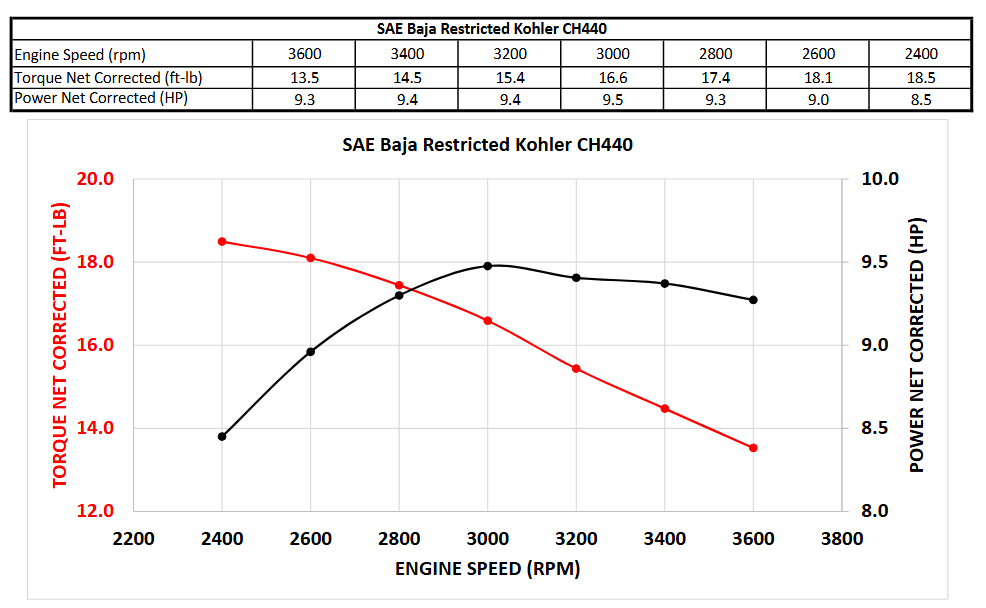
\includegraphics[width=0.72\textwidth]{figures/overview/kohler_ch440_torque_power_curve.png}}
\caption{Torque and power of the Kohler CH440 engine as functions of engine speed. 
Both quantities vary substantially across the operating range, with peak torque 
occurring at a lower engine speed than peak power. \citep{BajaSAEKohlerEngine2022}}
\label{fig:kohler_engine_motivation}
\end{figure}

\begin{figure}[H]
\centering
\fbox{
\begin{minipage}{1.00\textwidth}
\centering
\vspace{0.4cm}

\begin{minipage}[b]{0.46\textwidth}
\centering
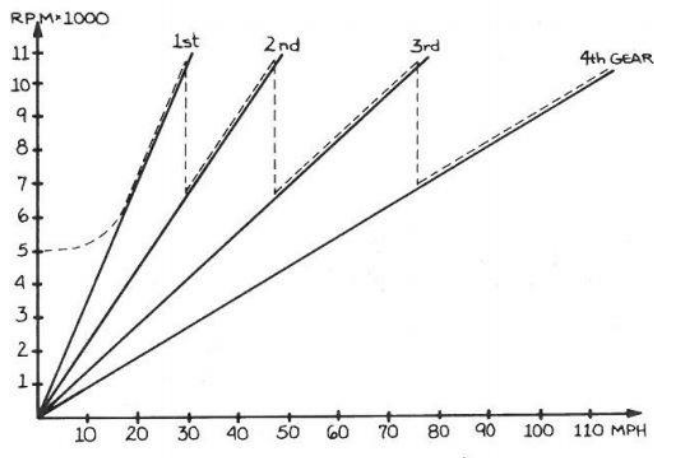
\includegraphics[width=\textwidth]{figures/overview/discrete_transmission_shift_curve.png}
\end{minipage}
\hfill
\begin{minipage}[b]{0.46\textwidth}
\centering
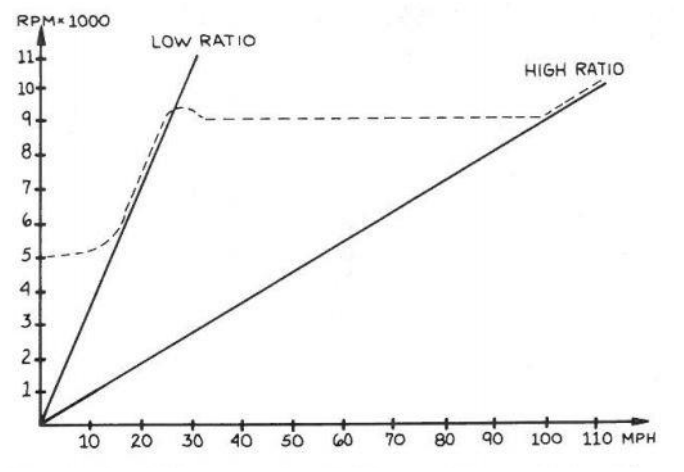
\includegraphics[width=\textwidth]{figures/overview/cvt_shift_curve.png}
\end{minipage}

\vspace{0.4cm}
\end{minipage}
}
\caption{Conceptual comparison of engine-speed behavior during acceleration. Solid 
lines show the engine-speed–vehicle-speed relationship imposed by the available 
transmission ratios, while the dotted line illustrates a representative engine-speed 
trajectory during acceleration. With a stepped gearbox (left), the engine repeatedly 
sweeps through a speed range and drops in speed at each gear change. With a CVT (right), 
engine speed can rise to a desired operating speed and remain approximately constant 
while the transmission continuously changes ratio, increasing again only after the 
high-ratio limit is reached. \citep{Aaen2007} }
\label{fig:transmission_shift_motivation}
\end{figure}


\subsection{Physical Layout and Single-Pulley Geometry}
\label{subsec:physical_layout_single_pulley}

There are several forms of continuously variable transmission, including
different mechanical layouts and different ways of producing the variable speed
relationship. This work focuses on a belt-sheave CVT, shown conceptually in 
\Cref{fig:cvt_system_overview}. In this arrangement, two variable-radius pulleys 
are connected by a rubber V-belt. The pulley connected to the engine
side is called the primary (or driving) pulley. The pulley connected to the
downstream drivetrain is called the secondary (or driven) pulley. The belt
transmits motion and torque between these two pulleys.

\begin{figure}[H]
\centering
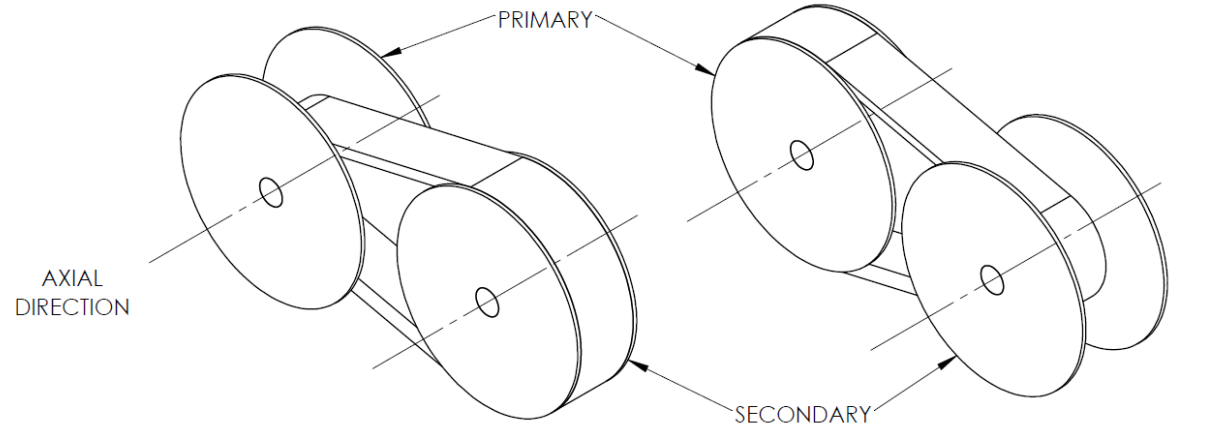
\includegraphics[width=\textwidth]{figures/overview/cvt_example.png}
\caption{Two sample configurations of the belt-sheave CVT considered in this work. 
The primary pulley is connected to the engine side, the secondary pulley is
connected to the downstream drivetrain, and the rubber V-belt transmits motion
and torque between them. \citep{Messick2018}}
\label{fig:cvt_system_overview}
\end{figure}


Before considering the full two-pulley system, it is helpful to look at the
geometry of a single pulley. Both the primary and secondary pulleys share the
same basic anatomy. Each pulley is made from two opposing conical sheaves that
form a V-shaped groove. One sheave is fixed axially to the shaft, while the
other can move along the shaft. The rubber V-belt sits between the sheave
faces. This basic layout is shown in \Cref{fig:single_pulley_anatomy}.

\begin{figure}[H]
\centering
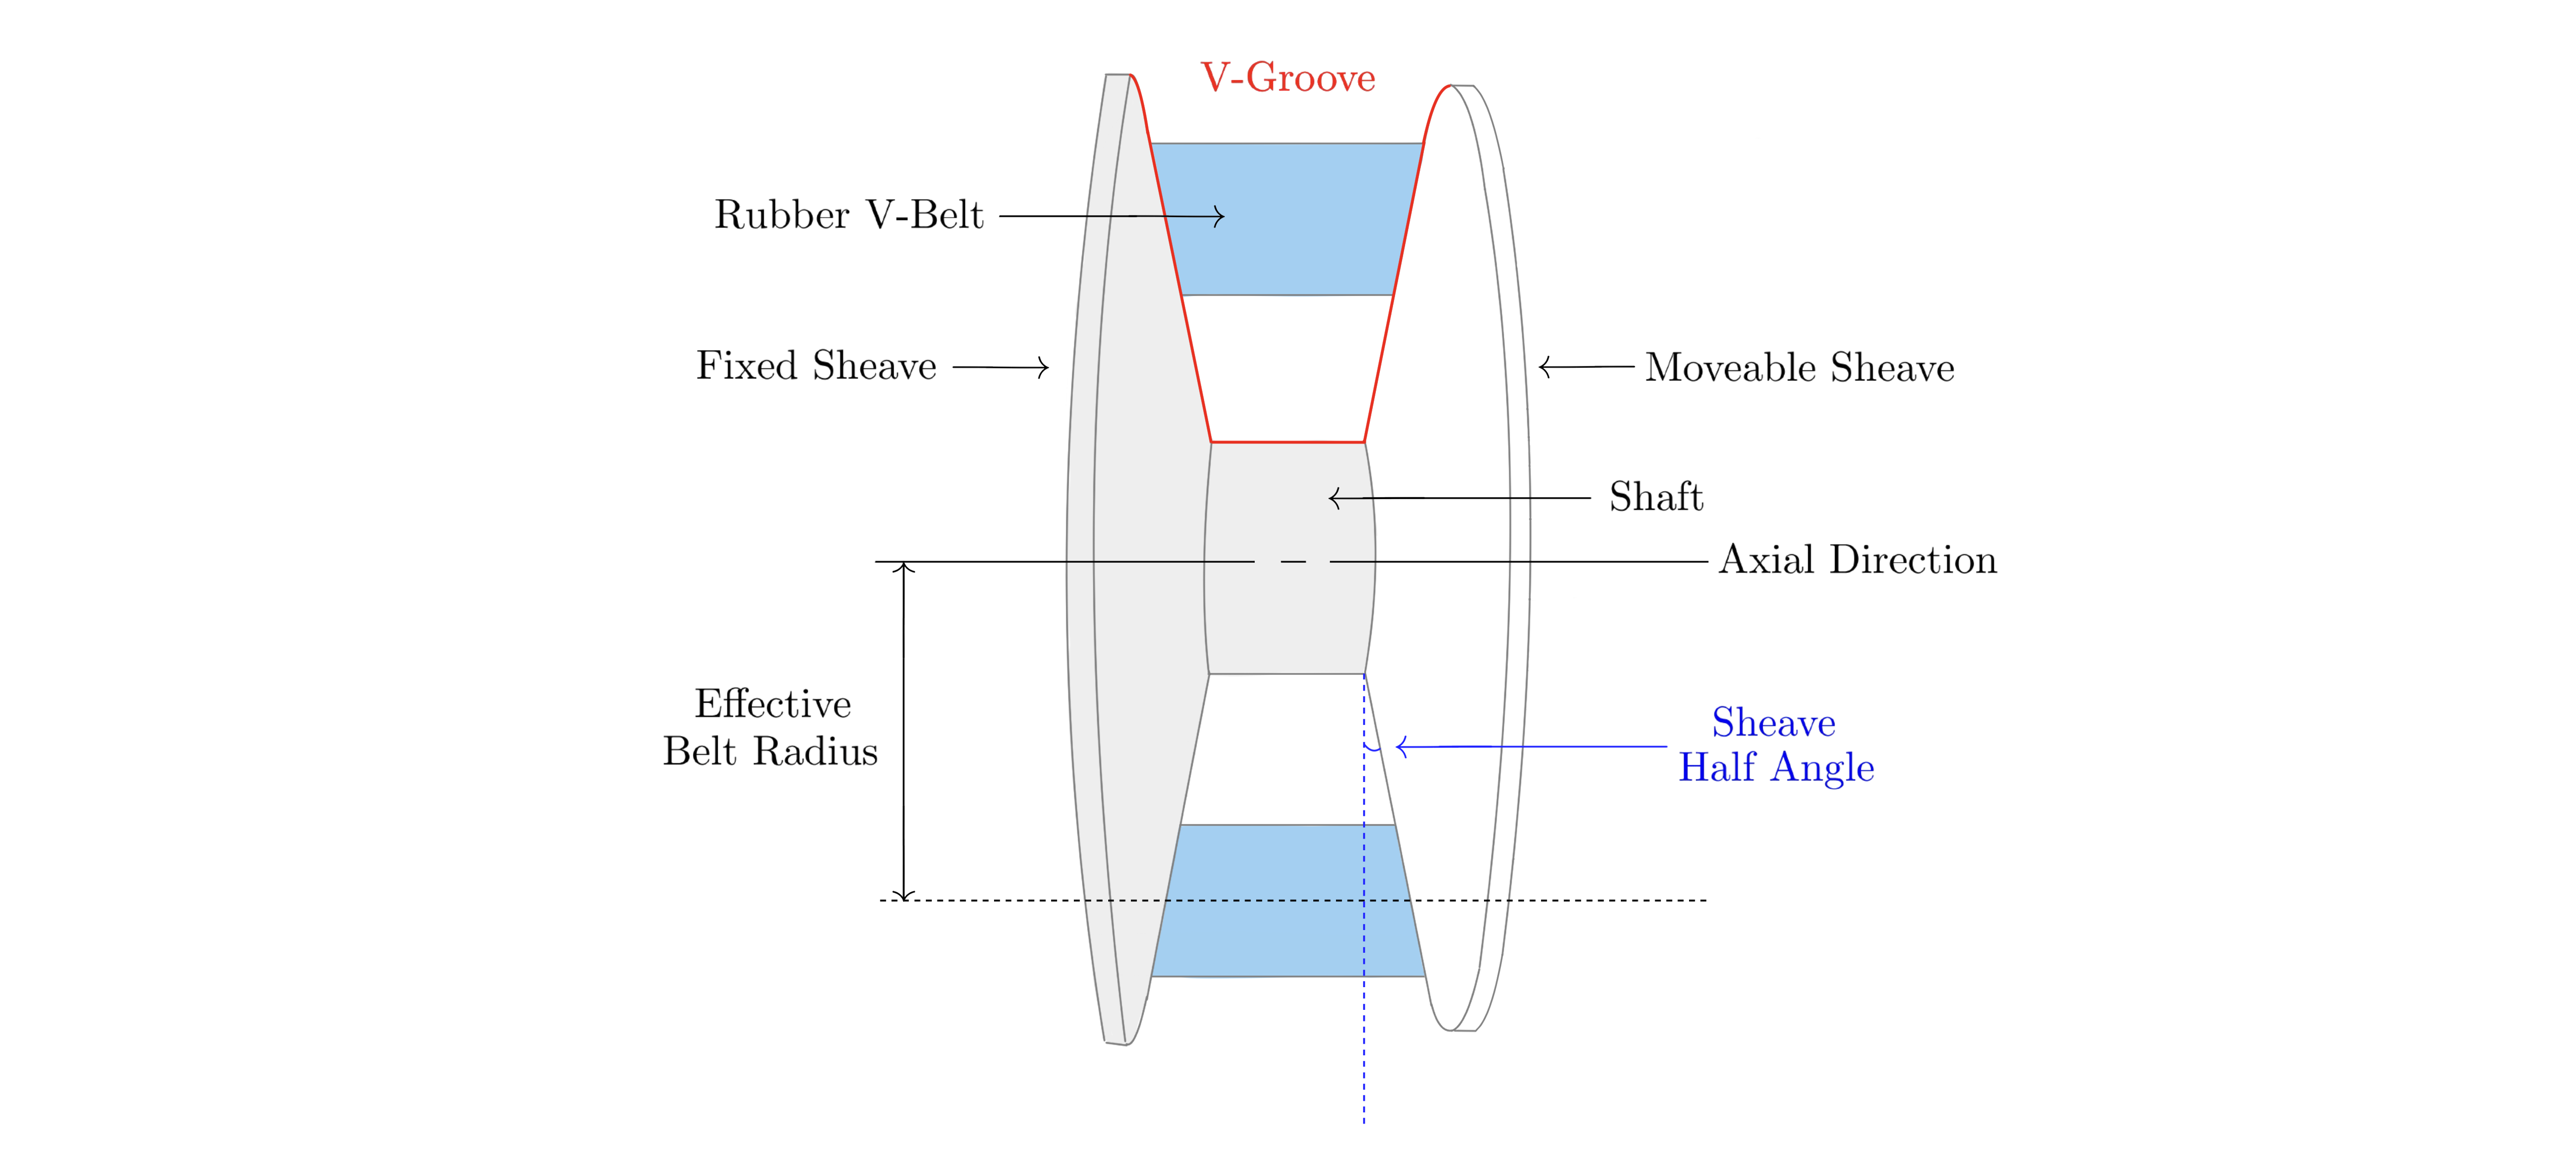
\includegraphics[width=\textwidth]{figures/overview/single_pulley_anatomy.png}
\caption{Generic anatomy of a belt-sheave CVT pulley. Each pulley consists of
opposing conical sheaves that form a V-groove. Motion of the movable sheave
changes the groove width and therefore changes the radius at which the belt
rides.}
\label{fig:single_pulley_anatomy}
\end{figure}

The key geometric idea is simple: changing the axial separation between the
sheaves changes the effective radius of the belt. If the movable sheave moves
toward the fixed sheave, the groove becomes narrower. Since the belt has a
finite width, it cannot occupy the same radial position in the narrower groove,
so it is pushed outward along the conical sheave faces. The effective belt
radius therefore increases.

If the movable sheave moves away from the fixed sheave, the groove becomes
wider and the belt can fall deeper between the sheaves. This reduces the
effective belt radius. At this level, the mechanism is just wedge geometry:
axial motion of the sheave becomes radial motion of the belt. Closing the
sheaves makes the belt radius larger, while opening the sheaves makes the belt
radius smaller, as shown in \Cref{fig:single_pulley_states}.

\begin{figure}[H]
\centering
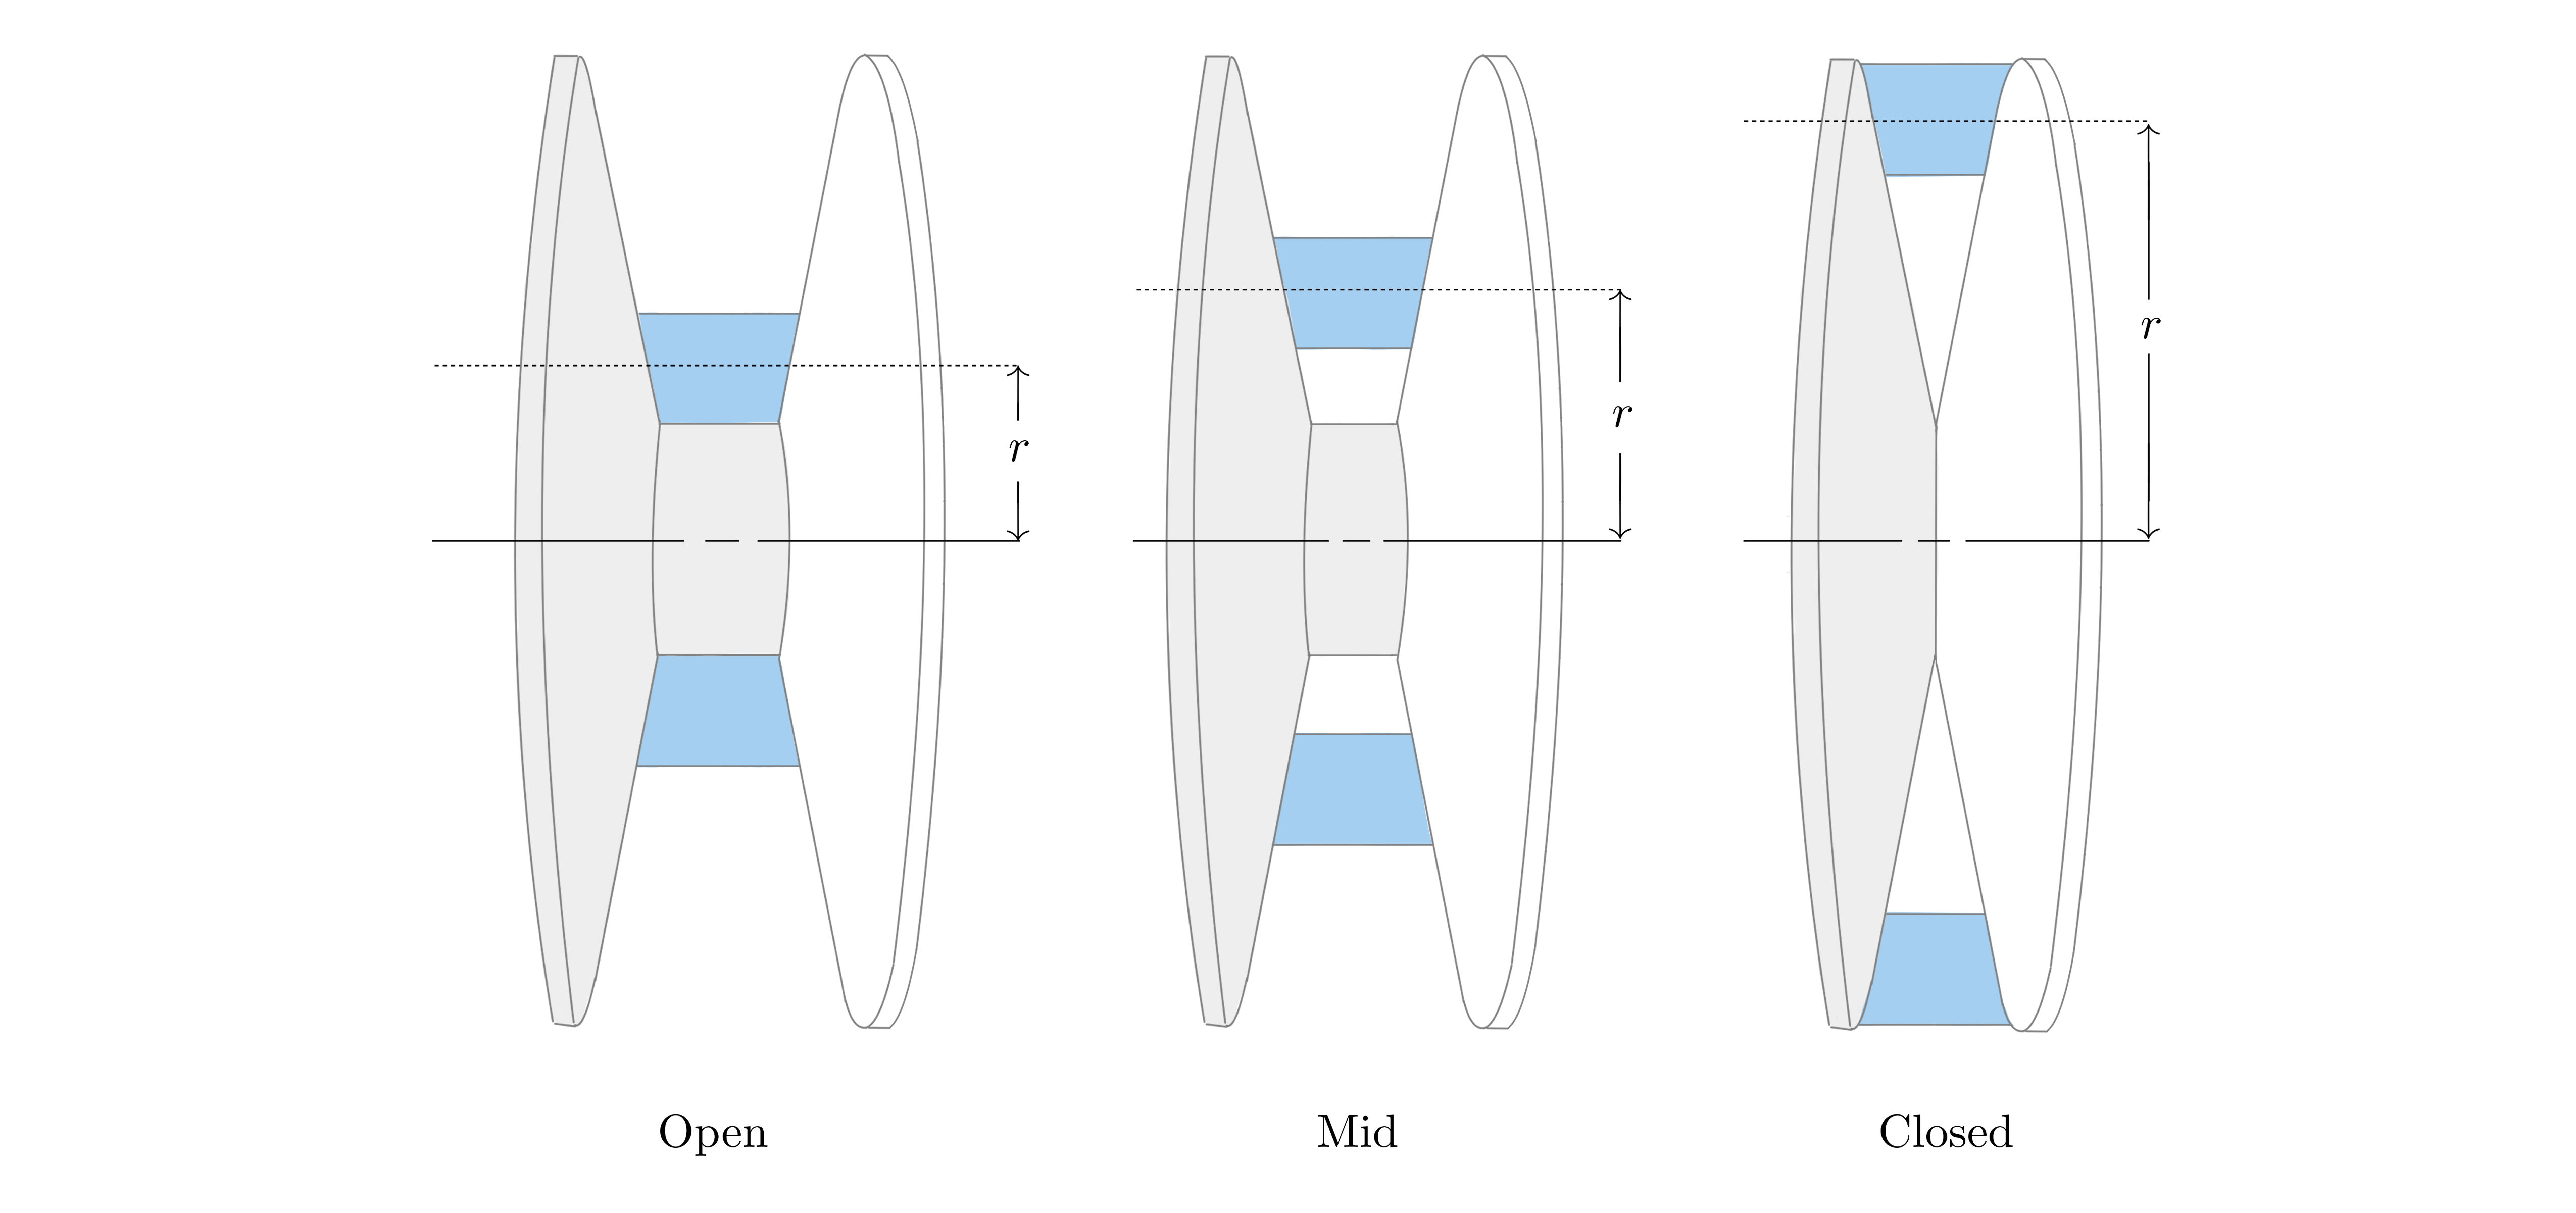
\includegraphics[width=\textwidth]{figures/overview/single_pulley_states.png}
\caption{Single-pulley radius change. As the sheaves close, the V-groove
narrows and the belt is pushed outward to a larger effective radius. As the
sheaves open, the belt can fall deeper in the groove and the effective radius
decreases.}
\label{fig:single_pulley_states}
\end{figure}

% --------------------------------------------------------------
\subsection{Two-Pulley Coupling and Ratio Change}
\label{subsec:two_pulley_coupling}

The full CVT contains two of the variable-radius pulleys described above. The
important difference is that the two pulleys are connected by the same belt.
Because the belt length is approximately fixed, the effective radii of the two
pulleys cannot change independently.

If the belt rides outward on the primary pulley, it must ride inward on the
secondary pulley. Likewise, if the primary radius decreases, the secondary
radius must increase. This opposite motion is the core geometric behavior that
allows the CVT ratio to change. In the physical mechanism, the actual motion of
the sheaves occurs through contact forces, springs, actuator mechanisms, and the
axial force balance of the pulleys.

The CVT begins launch in a low-speed, high-reduction configuration. In this
state, the primary pulley has a small effective radius and the secondary pulley
has a large effective radius. This behaves like a low gear in a conventional
drivetrain: the engine-side pulley turns relatively quickly while the downstream
side turns more slowly, amplifying torque through the drivetrain.

As the CVT upshifts, the primary sheaves close and the primary effective radius
increases. At the same time, the secondary effective radius decreases. The
transmission therefore moves from its launch configuration toward a
higher-speed configuration. By the end of the shift, the primary radius is
larger and the secondary radius is smaller. This coupled motion is shown in
\Cref{fig:cvt_ratio_states}.

\begin{figure}[H]
\centering
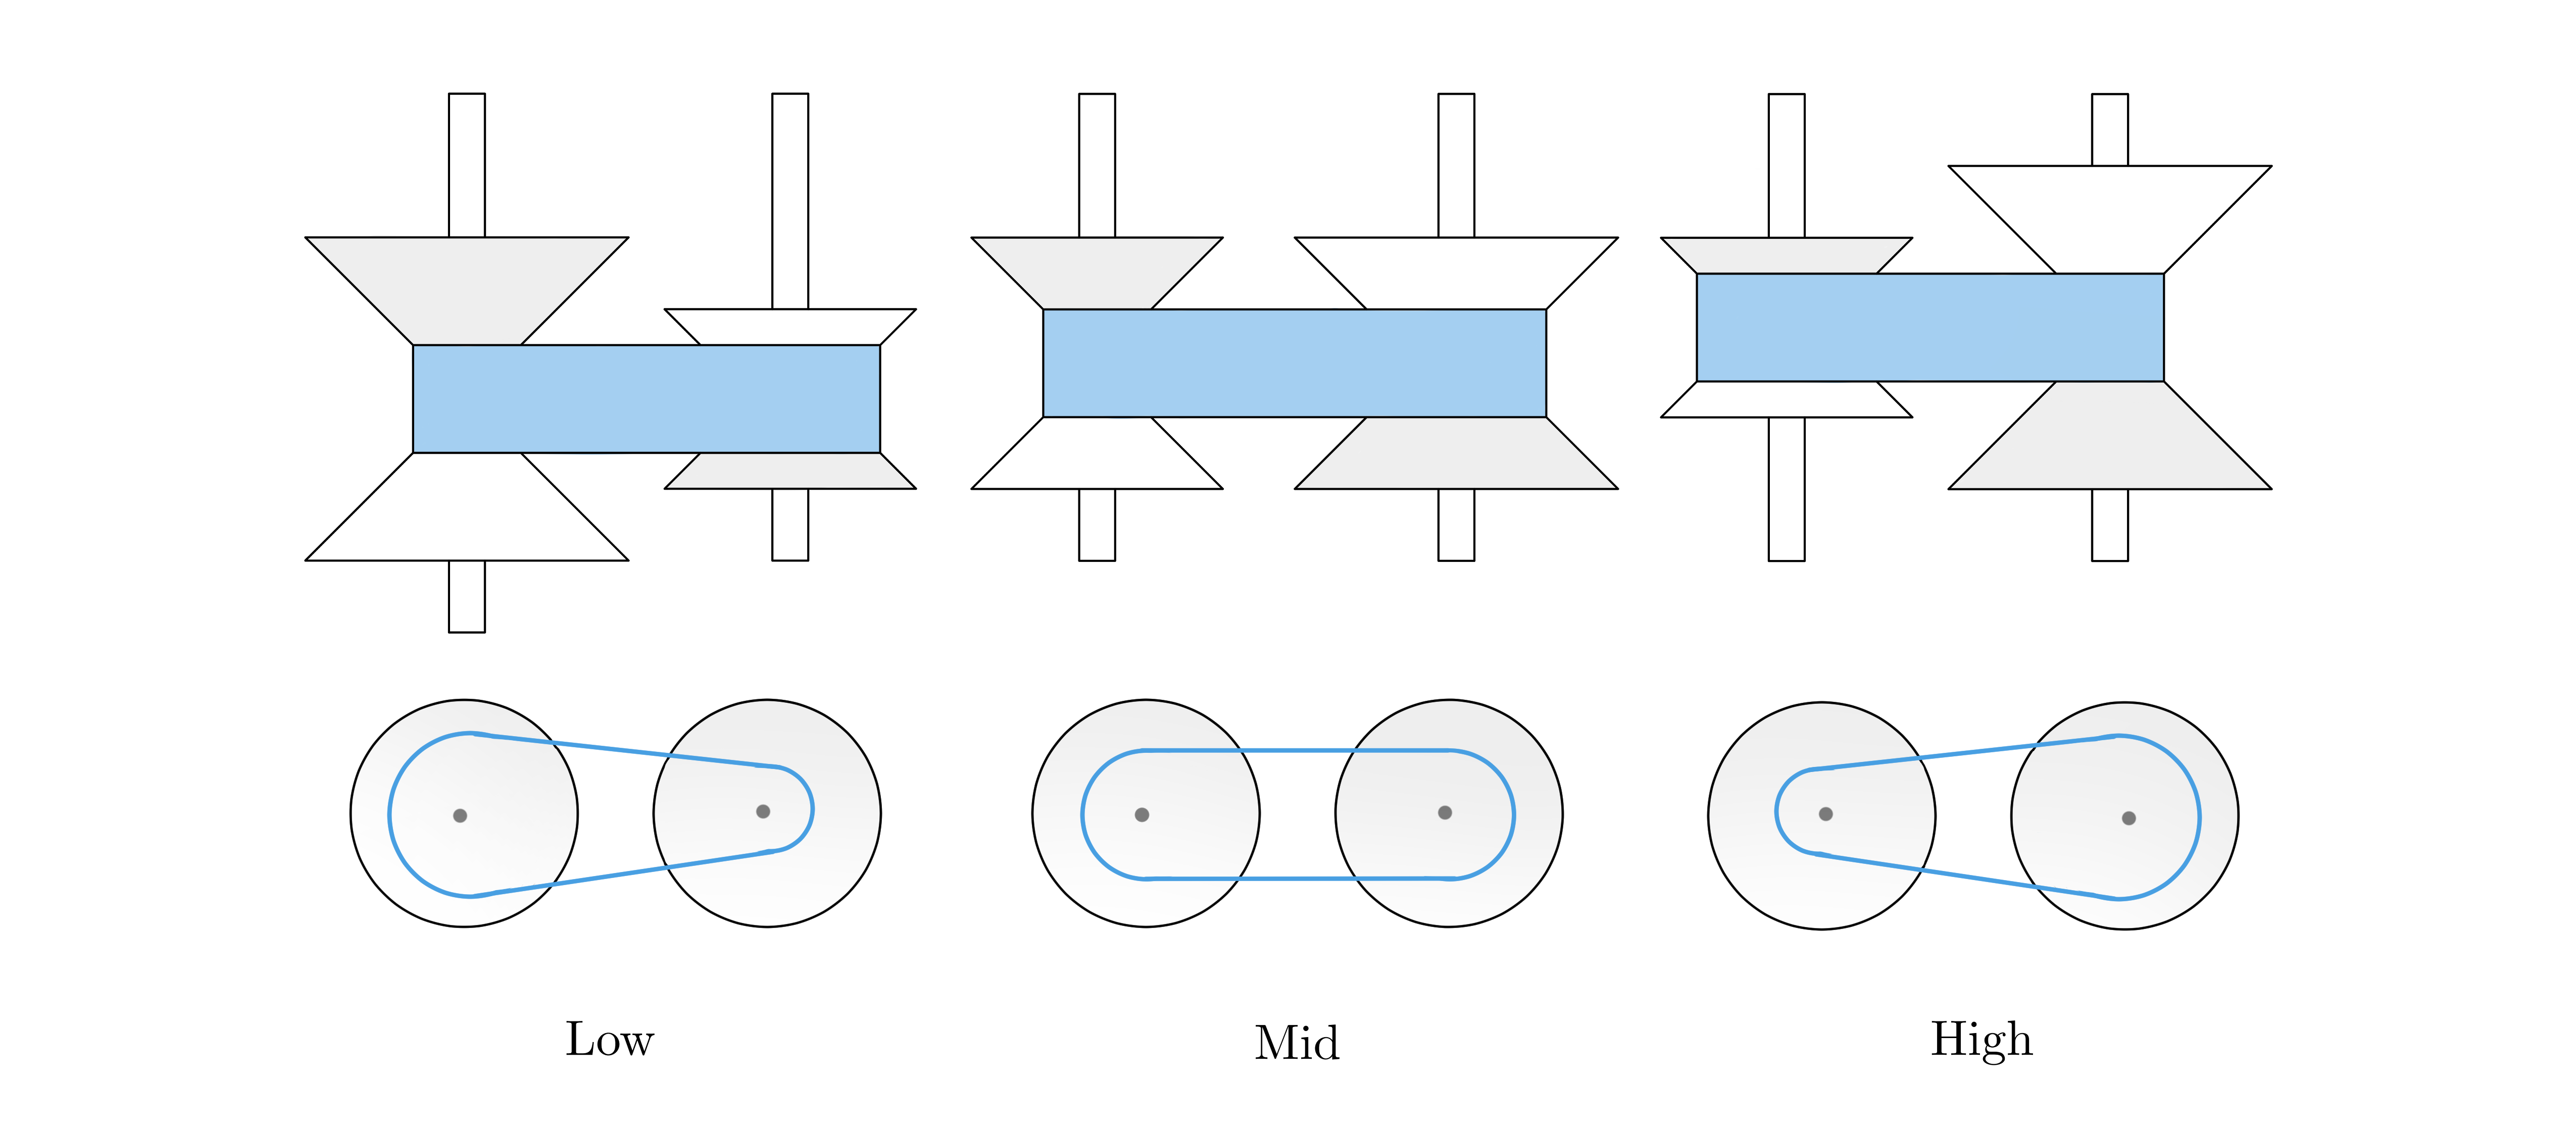
\includegraphics[width=\textwidth]{figures/overview/cvt_low_med_high_ratio.png}


\caption{Low-, intermediate-, and high-ratio states of a belt--sheave CVT. 
As the belt moves outward on the primary pulley and inward on the secondary pulley, 
the effective radii vary in opposite directions while the belt length remains 
approximately constant. The lower views highlight the corresponding change in 
transmission ratio.}
\label{fig:cvt_ratio_states}
\end{figure}

% --------------------------------------------------------------
\subsection{Torque Transfer, Clamping Force, and Slip}
\label{subsec:traction_and_slip}

The geometry described so far determines the speed relationship between the
primary and secondary pulleys. However, a speed relationship alone does not
guarantee that torque can be transmitted. Unlike a gear pair, the belt and
pulley are not mechanically locked together by teeth. Torque is transmitted
through frictional traction between the belt and the sheave faces.

For traction to develop, the belt must be physically squeezed between the
sheave faces. \Cref{fig:belt_sheave_forces} shows how this happens at a small
portion of the belt--pulley contact. The circled region on the pulley wrap is
enlarged to show the belt cross-section within the pulley V-groove. At that
location, the movable sheave presses the belt toward the fixed sheave. This
clamping action produces contact normal forces on the two sides of the belt,
creating the contact pressure needed for frictional traction.

The same local interaction occurs continuously around the wrapped portion of
the belt. At each position along the wrap, the normal forces between the belt
and sheave faces allow a tangential friction force to act. Together, these
small tangential traction forces transfer torque between the pulley and the
belt. In practical terms, transferring more torque through the CVT requires enough
clamping force to create enough available traction at the belt--pulley
interface. More clamping force increases the normal contact force, which in
turn increases the tangential force that friction can support.

\begin{figure}[H]
\centering
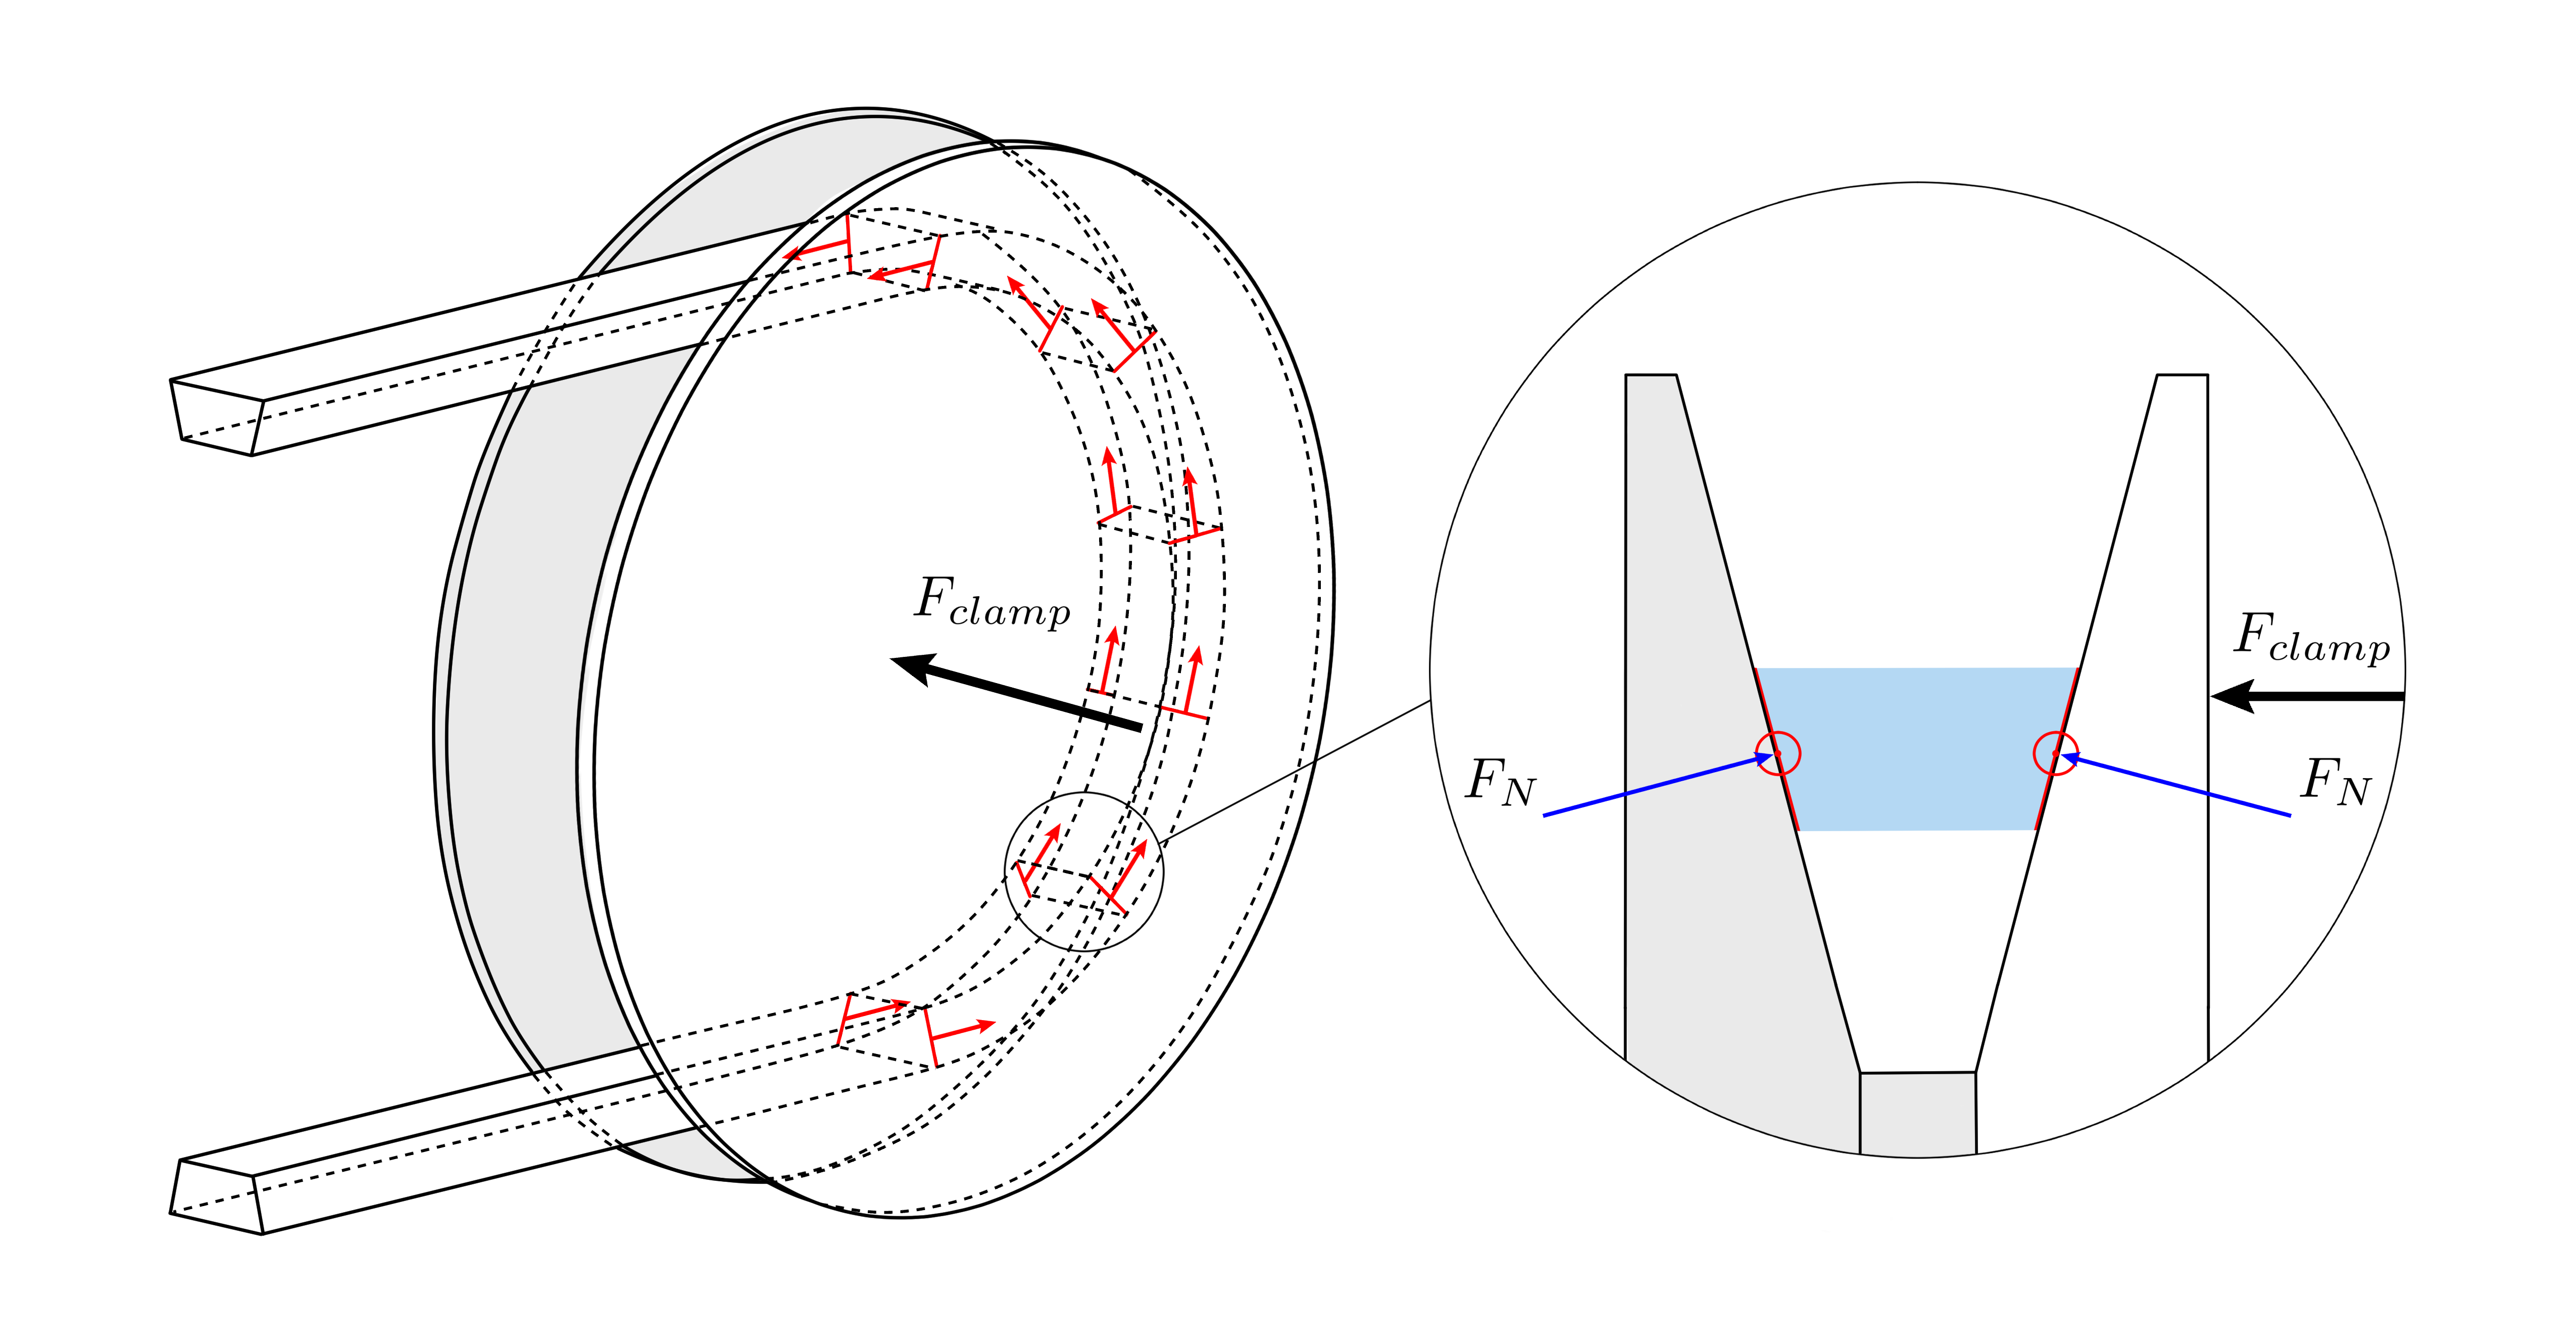
\includegraphics[width=\textwidth]{figures/overview/traction.png}
\caption{Clamping and traction in a rubber V-belt CVT. The axial clamping
force \(F_{\mathrm{clamp}}\) presses the movable sheave toward the fixed
sheave. At the circled location, the enlarged cross-section shows representative
local face-normal forces \(F_N\) acting on the belt. These normal forces set
the frictional capacity for the local tangential traction shown around the
wrap, whose distributed action transfers torque between pulley and belt.}
\label{fig:belt_sheave_forces}
\end{figure}

If the available traction is not sufficient for the torque being transferred,
the belt slips relative to the pulley. Slip reduces useful torque transfer and
can produce heat, wear, and efficiency loss. A working CVT must therefore do
two things at once: it must allow the pulley radii to change so the ratio can
shift, and it must maintain enough clamping force for the belt to transmit
torque without excessive slip.

This distinction is central to the rest of the model. The pulley geometry
determines how the speed ratio changes. The contact mechanics determine how
much torque can actually be carried through the belt--pulley contacts. A CVT is
therefore not only a variable-geometry mechanism; it is also a clamping and
traction problem.

\subsection{Mechanical Actuation in the Present CVT}
\label{subsec:cvt_actuation_overview}

Different CVTs generate radius change and clamping force in different ways.
Some systems use electronic or hydraulic actuation to command pulley motion or
clamping pressure directly. The system studied here is mechanically actuated:
its pulley forces arise from mechanisms inside the primary and secondary pulley
assemblies rather than from an externally commanded ratio.

These mechanisms are important because they determine both how the belt moves
through the ratio range and how much clamping force is available for torque
transfer. The primary pulley is mainly speed-sensitive, while the secondary
pulley is mainly torque-reactive.

The primary pulley uses flyweights, ramps, and a spring. As engine speed
increases, the flyweights move outward under centrifugal effects. The ramp
surfaces convert this outward flyweight motion into a closing force on the
primary sheaves. The spring resists this motion and helps set the speed at which
the primary begins to close. As the primary closes, the belt is pushed outward,
the primary effective radius increases, and the CVT shifts in the upshift
direction introduced in \Cref{fig:cvt_ratio_states}. The primary actuation
mechanism is shown conceptually on the left side of
\Cref{fig:cvt_mechanical_actuation}.

The secondary pulley uses a helix mechanism and spring loading. The helix can
be understood like a screw-like interface: when torque is transmitted through
the secondary, the angled helix surfaces convert part of that torque reaction
into a clamping force between the sheaves. In this way, torque through the
secondary helps create the clamping needed to carry torque through the belt.
The spring provides preload and helps set the baseline clamping behavior.

The helix also means that secondary shift is not purely axial. As the secondary
moves through its shift range, axial motion is coupled with relative rotation
between secondary sheave components. This detail becomes important later when
the secondary force model is developed, but the basic intuition is simply that
the helix converts torque and relative rotation into axial clamping. The
secondary actuation mechanism is shown conceptually on the right side of
\Cref{fig:cvt_mechanical_actuation}.

\begin{figure}[H]
\centering
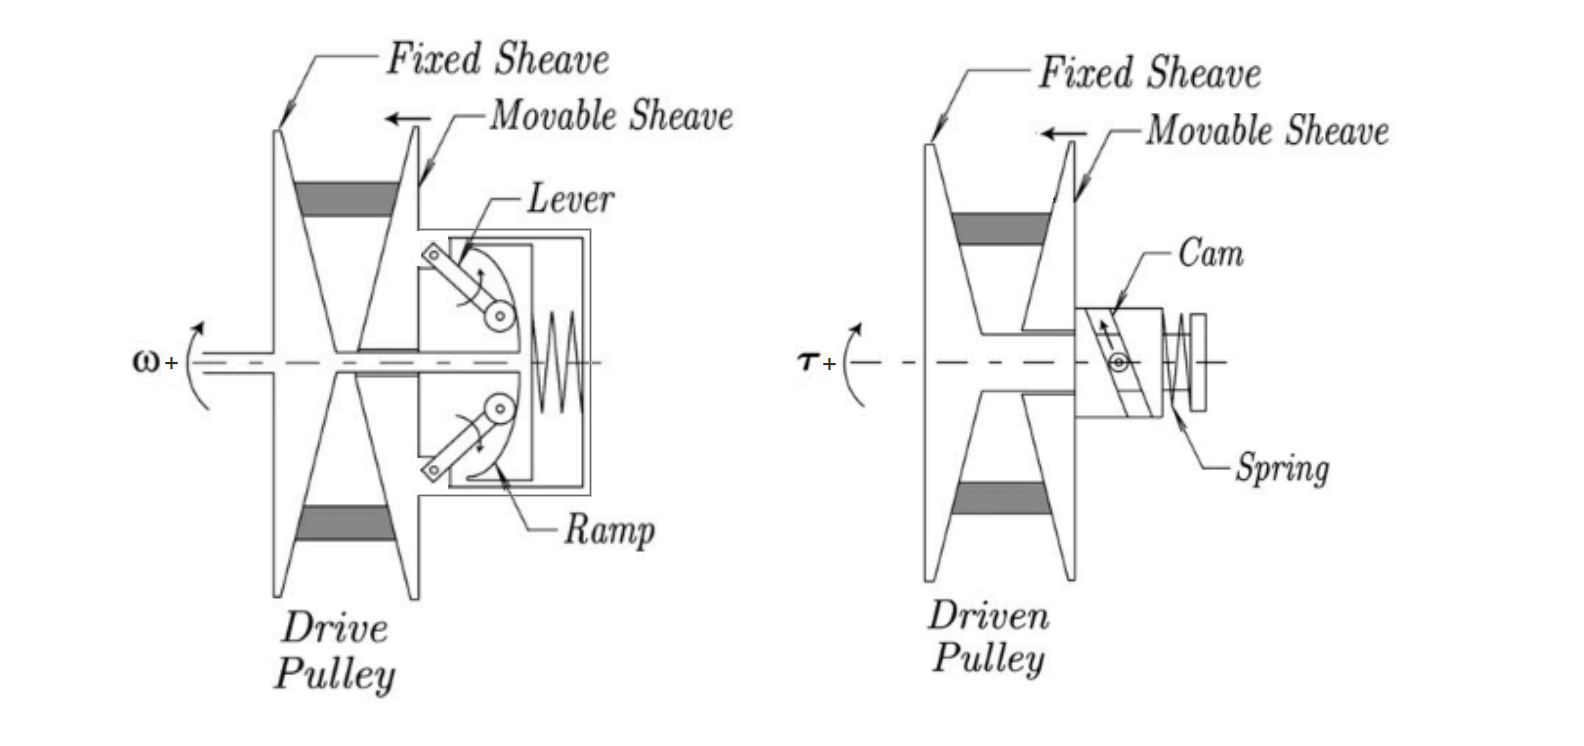
\includegraphics[width=\textwidth]{figures/overview/cvt_mechanical_actuation_concept.png}
\caption{Conceptual illustration of the mechanical actuation mechanisms in the
present CVT. Left: the primary (drive) pulley, where increasing rotational speed
moves the flyweights outward and the ramp geometry converts that motion into a
closing force on the sheaves, opposed by a spring. Right: the secondary (driven)
pulley, where transmitted torque loads a cam or helix mechanism that converts
part of the torque reaction into sheave clamping force, together with spring
preload. In this way, the primary is mainly speed-sensitive and the secondary is
mainly torque-reactive. \citep{JulioPlante2011}}
\label{fig:cvt_mechanical_actuation}
\end{figure}

Although the primary and secondary mechanisms respond most strongly to
different physical quantities, they act on the same belt and the same shift
process. Primary speed affects centrifugal actuation, transmitted torque affects
the torque-reactive secondary, the resulting clamping forces determine the
available belt traction, and the belt geometry couples motion of the two
pulleys. As the operating conditions change, the balance among these effects
can change as well, allowing the transmission to shift in either direction or
to enter a different traction state. These coupled relationships form the
physical foundation for the dynamic behaviour developed later in this work.

\section{Motivation and Literature Review}
\label{sec:literature-review}

CVT modelling is not a single, uniform problem. A model developed to size a variator, estimate belt efficiency, design a control strategy, or predict transient behaviour may involve the same physical components, but it will usually make different choices about which quantities are prescribed and which are solved. Some models are primarily design tools. Some focus on mechanical actuation and force balance. Some study belt forces, axial thrust, slip, or efficiency at fixed operating points. Others attempt to resolve transient shift behaviour or detailed belt--pulley contact mechanics.

The progression followed here is from design intuition, to component force balance, to mechanical actuation, to belt contact, to ratio change, and finally to general transient CVT behaviour. This ordering mirrors the way the modelling problem becomes difficult. A belt--sheave CVT can first be understood as a variable-radius transmission, then as a collection of mechanical actuators that generate axial force, then as a friction-limited belt contact problem, and finally as a coupled dynamic system in which pulley rotation, shift motion, belt behaviour, and contact state evolve together. The literature contains strong foundations for each of these pieces, but those foundations are distributed across several modelling traditions.

\subsection{Framework for Classifying CVT Models}
\label{sec:lit-classification}

A useful way to compare CVT models is to ask what part of the system is being allowed to move, and what part is being held fixed. The same physical transmission can be treated as a geometry problem, a force-balance problem, a belt-contact problem, a shift-dynamics problem, or a coupled system-dynamics problem. Each viewpoint can be useful, but each one answers a different question. This is why the literature is best read by tracking the modelling choices that define each formulation, rather than by treating all CVT models as attempts at the same final system.

One of the first choices is how the ratio is represented. In the simplest case, the transmission is evaluated at a fixed ratio. A slightly broader approach computes the ratio from a quasi-static force balance at each operating point. Other models prescribe a ratio trajectory, or use an empirical relationship for the rate of ratio change. More detailed shift models treat ratio change as a mechanical process in its own right, involving radial belt motion, pulley motion, and contact forces \citep{KimEtAl2002,Sorge2008,CammalleriSorge2009,SorgeCammalleri2011}. These approaches are not interchangeable. A fixed-ratio model can explain forces at a known condition, while a shift model can explain how the system moves from one condition to another. Even then, a formulation that describes the mechanics of an imposed or already active shift does not necessarily determine when a shift begins, which direction it takes, or what operating condition follows it.

A second choice is how axial force is produced. Some models take pulley clamping forces as known inputs. This is natural when the goal is to study belt response under specified loading, or when the variator is externally controlled. Other models include the mechanism that generates those forces, such as centrifugal weights, springs, torque-sensitive cams, hydraulic pressure, or electronic actuation \citep{Cammalleri2005,KimEtAl2002,Skinner2020,SorgeCammalleri2011}. The important distinction is not only the actuator type, but how completely its mechanical action is resolved. A clamping force may be prescribed directly, obtained from an instantaneous force balance or empirical relation, or produced by a mechanism whose own motion is treated dynamically. Each choice answers a different question about how the pulley force arises.

A third choice is how much of the belt--pulley contact is represented. At low fidelity, the belt may be treated through a capstan-style tension relation, often adjusted for the wedge action of the V-groove. More detailed models include radial and tangential friction, sliding angle, belt penetration, bending stiffness, local normal pressure, tension variation, slip mechanisms, and efficiency losses \citep{Gerbert1996,KimKim1989,Sorge1996,KongParker2005,KongParker2006,ChenLeeSung1998,Bertini2014,Messick2018}. At still higher fidelity, the belt may be discretized into nodes or elements so that local belt motion and contact behaviour are solved directly \citep{JulioPlante2011,Ballew2015}. Increasing contact fidelity can make the local mechanics more realistic, but it does not by itself determine how much of the complete transmission response is being solved. Local mechanical fidelity and global dynamic closure are therefore separate modelling choices.

A fourth choice is how the rotating system and its interaction with the surroundings are treated. Many models prescribe one or both pulley speeds, or impose the speed ratio algebraically. This is often appropriate for steady contact analysis, efficiency prediction, or controlled operating-point studies. Other models solve rotational equations of motion so that pulley speeds and transmitted torques evolve dynamically \citep{SrivastavaHaque2007,Ballew2015,DuanEtAl2016}. Any physical transmission must, of course, interact with whatever machinery is attached to it. The important distinction is whether those external systems supply only the mechanical loading associated with that interaction, or whether quantities belonging to the internal CVT mechanics---such as pulley-speed histories, clamping-force histories, axial pulley motion, or ratio trajectories---must also be prescribed. This distinction determines how much of the transmission operating state is actually predicted by the model.

A further choice is the operating region over which the same formulation remains valid. Some models are intended for steady or fully engaged operation. Others describe transient shifting once the variator is already engaged, focus specifically on clutching or engagement, or move through a predefined sequence of operating phases. A broader formulation must determine which mechanical regime is active as conditions change and remain valid as the transmission enters or leaves those regimes. A model may therefore reproduce behaviour accurately within one operating phase without necessarily providing the mechanics that determine how the transmission reaches, leaves, or reverses that phase.

These questions form a useful progression for understanding the modelling problem, but the associated modelling choices are partly independent. A formulation may resolve belt contact in great detail while prescribing global pulley motion. Another may solve pulley rotation dynamically while receiving clamping force as an external input. Another may model mechanical actuation carefully while treating ratio change through quasi-static or empirical relations. None of these choices is inherently wrong; they reflect the intended modelling objective. The important point is that model fidelity in one part of the CVT does not by itself imply closure of the complete transmission response.

The following review therefore considers both what each formulation was developed to predict and what quantities or operating conditions remain prescribed. It proceeds from practical and quasi-static design models, through mechanical actuation and belt-contact mechanics, to transient rubber-belt formulations and related dynamic models in metal-belt and chain CVTs. This provides a consistent basis for identifying which parts of the CVT dynamics are already well established and where the remaining modelling gaps lie.


\subsection{Practical Design and Tuning Foundations}
\label{sec:lit-practical-design}

The practical understanding of mechanically actuated rubber V-belt CVTs developed largely through machine design and tuning practice. General machine design references such as \citet{BudynasNisbett2015} provide the background needed to treat the CVT as a real mechanical assembly involving belts, springs, clutches, shafts, friction interfaces, uncertainty, and design iteration. Not all of these effects are included in a compact model, but they provide useful context for deciding which behaviours are retained and which are idealized.

Practical tuning literature provides a more application-specific foundation. \citet{Aaen2007} describes powersport CVTs using the language of engagement speed, shift speed, flyweights, primary springs, secondary springs, torque sensing, backshift, and speed variance. Its value is not that it provides a complete dynamic model, but that it builds component-level intuition from the perspective of a tuner or racer. It explains how changes to weights, springs, ramps, and helices are expected to affect behaviour, while leaving much of the coupled system response to experience and testing.

These sources are valuable because they describe the physical machine before it is reduced to equations. They also show why prediction is difficult: the same hardware change can affect engagement, shift rate, belt grip, backshift, engine speed, and vehicle acceleration at the same time. Qualitative tuning rules are therefore useful starting points, but they are not enough to determine the complete transient response of the CVT under changing operating conditions.

\subsection{Design-Oriented and Quasi-Static CVT Models}
\label{sec:lit-design-models}

Design-oriented CVT models commonly evaluate the transmission at a fixed operating condition or through a sequence of quasi-static operating points. Rather than asking how every transient state evolves in time, these models usually ask which geometry, actuator, belt, or tuning parameters should be selected to satisfy a desired operating requirement. In a fixed-operating-point analysis, quantities such as ratio and pulley speed may be specified while the corresponding forces, tensions, or capacities are calculated. In a quasi-static model, the operating condition may instead be obtained from an instantaneous force balance, while inertia and the time required to move between neighbouring equilibria are neglected. These approaches commonly relate vehicle requirements, pulley geometry, belt length, wrap angle, speed ratio, flyweight force, spring preload, helix force, belt tension, and torque capacity. Their main value is that they connect tunable hardware to expected operating behaviour.

A useful starting point is the numerical design method of \citet{ArangoMunoz2020}, which begins from vehicle requirements, road specifications, and desired performance before working toward the CVT design. This is valuable because it places component selection in its proper context: the belt, pulley geometry, speed-ratio range, engine or motor selection, and mechanical centrifugal actuation are not independent choices, but responses to the requirements imposed by the vehicle and its operating route. In this sense, the work provides a design-level framework where system requirements drive CVT component choices.

Other design-oriented works focus more narrowly on particular parts of the variator design. \citet{Cammalleri2005} develops a speed-torque-controlled rubber V-belt variator design using equilibrium relationships for a centrifugal driver and torque-sensitive driven pulley. \citet{LaBattaglia2022} focuses on the kinematic design of motorcycle rubber V-belt CVTs, emphasizing the roller sliding profile of the front pulley as a critical design variable. Both works show how simplified mathematical models can be used to choose actuator or geometry parameters without requiring a complete transient simulation of the transmission.

\citet{Skinner2020} provides a practical force-balance and tuning-oriented model. The work emphasizes quantifiable tuning objectives such as engagement speed, shift-out speed, static RPM shifting, and efficient power transfer, and relates those objectives to the primary and secondary subsystems. It is useful as an applied tuning reference because it connects the variables adjusted by teams to predicted operating behaviour, while remaining primarily an operating-point and force-balance model.

The common strength of these works is that they make CVT design less arbitrary. They identify the parameters that matter and show how geometry, springs, flyweights, helices, belt forces, and vehicle requirements can be related. They also highlight a recurring tension in CVT modelling: models that are simple enough to support early design may omit important coupled behaviour, while models that resolve more detailed mechanics can become difficult to apply directly as design tools. In this sense, design-oriented and quasi-static models occupy an important middle ground. They provide usable relationships for component selection and tuning, but they do not generally determine the complete time evolution of engagement, traction, shift motion, and pulley response.

\subsection{Mechanical Actuation and Clamping Force Generation}
\label{sec:lit-actuation}

After the basic design variables are identified, the next modelling question is how the CVT generates the axial forces that clamp the belt and drive ratio change. In externally controlled CVTs, these forces may be treated as prescribed hydraulic or electronic inputs. In mechanically actuated rubber V-belt CVTs, however, the forces are produced by the hardware itself. The primary force is typically speed-sensitive, while the secondary force is torque-sensitive.

\citet{Cammalleri2005} provides an important design treatment of this problem through a speed-torque-controlled rubber V-belt variator. The centrifugal driver and torque-sensitive driven pulley are treated as part of the variator design, with equilibrium relationships connecting actuator geometry, spring loading, pulley torque, and the intended operating behaviour of the CVT. This establishes a quantitative link between the mechanical hardware and the clamping forces it is designed to produce.

\citet{KimEtAl2002} also study a rubber belt CVT with mechanical actuators, including both steady-state and transient characteristics. Their driver and driven thrusts are obtained from the mechanical actuator geometry and instantaneous force balances, while the transient ratio response is represented separately by an experimentally identified first-order relationship. The work therefore connects mechanical primary and secondary actuation to transient CVT behaviour, but the motion of the actuator hardware itself is not what determines the shift acceleration.

\citet{SorgeCammalleri2011} address the secondary side in substantially greater mechanical detail through the helical shift mechanics of rubber V-belt variators. Their formulation allows the fixed and movable driven faces to rotate differently and resolves how the belt-contact state determines the torque carried by the movable face. The resulting helix response therefore depends on spring loading, helix geometry, transmitted torque, and the internal relative motion of the driven pulley rather than on a simple assumed torque split. The instantaneous pulley radius and shift speed are nevertheless supplied to the contact calculation, so the resulting actuator relation determines the forces associated with a specified shift state rather than the acceleration of the movable secondary assembly itself.

Together, these works establish much of the mechanical foundation needed to model passive CVT actuation. They show how centrifugal primary mechanisms and torque-reactive secondaries generate configuration-dependent axial forces, and how detailed actuator geometry can materially change those forces. They also illustrate an important distinction introduced in \Cref{sec:lit-classification}: including the actuator mechanism does not necessarily mean that the actuator is itself a dynamically propagated subsystem. In these formulations, the actuator force is generally closed configuration by configuration, while transient ratio motion is either outside the model or supplied through a separate shift description. This distinction becomes important when the actuator hardware has inertia and its motion is coupled directly to the shift and shaft dynamics.

\subsection{Rubber V-Belt Contact, Slip, and Efficiency Models}
\label{sec:lit-contact-efficiency}

Once axial force is generated by the actuation mechanisms, the belt-pulley interface determines what that force actually does. The sheaves may clamp the belt, but the resulting torque capacity, axial reaction, radial belt motion, slip, and loss all depend on how the rubber belt interacts with the pulley groove. A rubber V-belt therefore cannot be treated as an ideal kinematic constraint. It wedges into the sheaves, develops a tension distribution around the wrap, experiences radial and tangential friction, deforms under load, and dissipates energy through several mechanisms.

Classical belt theory gives the starting point: friction and wrap angle determine the maximum tension ratio that can be supported before gross sliding occurs. For V-belts, this picture is modified by the groove angle and the associated wedge effect. However, real belt slip is more complicated than a single capstan-style traction limit. \citet{Gerbert1996} presents a unified treatment of belt slip in which creep, radial compliance, shear deflection, and seating/unseating effects all contribute to speed loss. The important point is not that every model must include all of these effects, but that ``slip'' is not one physical mechanism. A model should be clear about which slip and loss mechanisms it represents and which it leaves outside its scope.

The contact problem also determines the axial reaction felt by the sheaves. \citet{KimKim1989} developed a theoretical analysis of axial forces in a rubber V-belt CVT using simplified assumptions about the contact regions and belt force distribution. \citet{Sorge1996} developed a compact model for axial thrust in V-belt drives, emphasizing radial penetration and the connection between belt forces and pulley thrust. These works are useful because they connect the belt contact state back to the sheave force balance: axial force is not only generated by the actuator, but also shaped by how the belt seats, slides, and transmits load in the groove.

A more detailed treatment is given by \citet{KongParker2005}, who formulate the steady mechanics of belt-pulley systems using distributed belt equations. \citet{KongParker2006} extend this framework to pulley grooves and sliding friction. This line of work resolves local belt mechanics at much greater fidelity than simple force-balance models, including the distribution of forces and sliding behaviour around the contact arc.

\citet{Messick2018} extends this contact-mechanics tradition for rubber V-belt CVTs by building on the Kong and Parker framework and validating axial-force and efficiency predictions experimentally. Messick's work is valuable for its contact-region formulation, belt property measurement, operating-range analysis, and dynamometer validation. It is also clear about its modelling scope: shifting is treated as a quasi-equilibrium process rather than as a transient response-time problem. In this sense, it is a strong reference for belt force and efficiency modelling, while leaving the time evolution of the complete CVT operating state to a different class of model.

Efficiency-focused studies provide another view of the same interface. \citet{ChenLeeSung1998} experimentally investigated speed and torque losses in a rubber V-belt CVT, while \citet{Bertini2014} developed an analytical model for rubber V-belt CVT power losses including sliding, hysteresis, and entry/exit effects. These works show that transmission losses arise from several interacting mechanisms whose relative importance depends on the operating condition.

The contact and efficiency literature therefore provides the foundation for understanding how belt force, axial thrust, slip, and loss arise. It also reinforces the distinction between local fidelity and global dynamic closure. A high-fidelity contact model may be necessary for efficiency prediction, axial-force prediction, or detailed local belt mechanics. A lower-dimensional contact model may instead be appropriate when the modelling objective requires the belt to remain coupled transparently to actuator dynamics, pulley rotation, shift motion, and the broader transient operating state of the CVT.

\subsection{Transient Rubber-Belt Models and Dynamic Closure}
\label{sec:lit-transient-rubber}

The contact and force-balance literature establishes how a rubber belt CVT behaves at a specified operating condition. Transient models extend this picture by asking how the transmission moves between operating conditions and which parts of that motion must be resolved in time. In the rubber-belt literature, this has been approached through models of shift mechanics, distributed belt motion, pulley rotational dynamics, and mechanically actuated vehicle response. A useful comparison among these works is therefore which parts of the CVT state are advanced dynamically and which quantities are supplied as operating conditions or inputs.

\citet{Sorge2008} provides an important bridge from quasi-static analysis to transient shift mechanics. Rather than representing ratio change as a sequence of neighbouring equilibria, the formulation treats the radial migration of the belt through the pulley grooves as a time-dependent process coupled to circumferential belt motion, mass conservation, and sliding. \citet{CammalleriSorge2009} later develop approximate closed-form solutions for the same class of shift problem. These works establish a mechanical basis for transient ratio change, while taking the pulley loading and active shift condition as part of the problem definition.

A more detailed transient treatment is given by \citet{JulioPlante2011}, who discretize the rubber belt and apply Newton's law to the individual belt elements. Their model predicts the time response of transmission ratio under specified drive-pulley axial force, drive-pulley speed, and load torque, while resolving belt elasticity, bending, damping, and frictional contact directly. The formulation is validated for steady and shifting conditions and provides substantially greater local belt detail than reduced force-balance models. The authors also report difficulty obtaining a stabilized prediction for the low-torque start-up condition in which belt clamping itself acts as the clutch, indicating that the operating range of the formulation is narrower than the full sequence of CVT engagement and shift behaviour.

\citet{Ballew2015} extends this discretized-belt model family by removing the prescribed input-pulley speed used in earlier formulations. Applied torques, pulley inertias, and belt forces instead determine the pulley angular accelerations, allowing both shaft speeds to evolve dynamically. Engine and vehicle submodels are also included so that changes in external loading can feed back through the transmission rather than being represented by a prescribed pulley-speed history.

Axial actuation in \citet{Ballew2015} remains a separate input to the belt--pulley model. The thesis notes that the axial-force inputs could be supplied either by a control system or by a model of a mechanically governed actuator. In the simulations presented, a PI controller with feed-forward gain generates the primary axial force, while the secondary axial force is held fixed. The formulation therefore extends the dynamic closure of the rotating system substantially, while leaving the source of the pulley clamping forces to a separate actuation model.

\citet{SilvaEtAl2023} present a reduced mechanically actuated rubber-belt CVT model coupled to a longitudinal vehicle simulation. Axial equations of motion are written for the movable sheaves, with flyweight loading on the primary and a torque-dependent secondary contribution. The operating sequence is divided into a clutching phase followed by a fully engaged phase, and the model is validated against a full-throttle acceleration. The work therefore provides an example of movable-sheave dynamics and mechanical actuation being retained in a transient application, while using a simplified, phase-specific representation of the CVT behaviour.

Taken together, these works show a clear progression in transient rubber-belt modelling. Ratio change has been treated as a mechanical process, belt motion and contact have been propagated directly, pulley rotational motion has been allowed to respond to applied torques, and movable-sheave inertia has been introduced in mechanically actuated applications. The formulations differ, however, in which parts of the transmission remain prescribed or are restricted to a particular operating phase. This makes the broader CVT literature useful for examining how other variator architectures have divided the boundary between prescribed actuation and dynamically resolved transmission behaviour.

\subsection{Adjacent Metal-Belt and Chain CVT Dynamic Models}
\label{sec:lit-metal-chain}

The broader CVT literature contains an extensive modelling tradition for metal push-belt and chain variators, particularly in automotive applications. These systems are not direct equivalents of dry rubber V-belt CVTs, since their load-carrying mechanisms, deformation, lubrication, and actuation systems differ. They nevertheless provide useful comparisons for transient ratio change, frictional contact, pulley dynamics, and the treatment of applied clamping forces.

\citet{SrivastavaHaque2009} review the dynamics and control of belt and chain CVTs and summarize a wide range of steady and transient formulations, including slip and traction models, control-oriented shift laws, and detailed belt or chain mechanics. The review illustrates both the maturity of dynamic CVT modelling outside the rubber-belt literature and the importance of keeping the underlying transmission architecture in view when comparing models.

The Carbone--Mangialardi--Mantriota (CMM) family provides a well-developed example of mechanically derived shift dynamics for metal-belt and chain variators. \citet{CarboneMangialardiMantriota2001,CarboneMangialardiMantriota2005} derive ratio-changing behaviour from belt or chain kinematics, mass conservation, friction, and pulley deformation, including creep-mode and slip-mode shifting. Experimental work by \citet{YildizEtAl2018} validates the resulting CMM shift dynamics under load. In these tests, the predicted quantity is the speed-ratio response to a prescribed change in clamping-force ratio, while drive-pulley angular speed, driven-side clamping force, and load torque are specified operating quantities. The formulation is therefore directed at the variator shift response under known actuation and loading.

Other metal-belt studies similarly treat transient ratio change and traction behaviour directly. \citet{SrivastavaHaque2005,SrivastavaHaque2008} develop dynamic formulations that retain transient belt motion and examine the effects of friction characteristics and band-pack slip. \citet{Bonsen2003} study variator slip and its relationship to transmitted torque and clamping. These works extend the treatment of shift and traction beyond steady operating-point analysis while retaining the controlled clamping architecture typical of metal-belt automotive CVTs.

\citet{SchindlerEtAl2012} develop a spatial transient multibody model of a pushbelt variator with detailed representation of the pulley sheaves, ring packages, friction, and unilateral contact. The model is used to study the internal transient response of the pushbelt system, including deformation and three-dimensional contact behaviour. In the simulations presented, the output pulley receives prescribed clamping force and load torque, while the input pulley is assigned angular-velocity and clamping-velocity histories. The detailed belt and pulley response is therefore resolved under a specified global variator excitation.

Chain CVTs provide another example of strongly coupled transient mechanics. \citet{DuanEtAl2016} include pulley rotational dynamics, movable-pulley axial dynamics, chain radial motion, chain and pulley deformation, and a speed-dependent friction model spanning micro-slip and macro-slip. The axial and rotational pulley dynamics are coupled directly through the chain forces. The movable-pulley equation is driven by an applied clamping force, however, so the generation of that clamping force remains outside the variator model.

These adjacent models show how transient shift mechanics, detailed contact behaviour, pulley rotation, and movable-pulley motion can be represented at substantially different levels of detail. They also illustrate a recurring modelling boundary: in hydraulically or otherwise externally actuated variators, clamping force and pulley actuation are naturally supplied as inputs to the transmission model. For a mechanically actuated rubber V-belt CVT, those same functions are produced by hardware contained within the transmission, making the treatment of the actuation mechanism itself an important part of how the model boundary is defined.

\subsection{Synthesis of Prior Work}
\label{sec:lit-synthesis}

The literature does not point to a single missing ingredient in CVT modelling.
Instead, several mature lines of work resolve different parts of the same
machine. Practical and design references establish the component relationships
used to size and tune rubber V-belt CVTs. Mechanical-actuation studies explain
how centrifugal and torque-reactive hardware generate pulley forces. Contact
and efficiency models resolve the belt--pulley interface at progressively
greater local detail. Transient formulations add radial belt motion, ratio
change, pulley rotation, movable-sheave dynamics, or distributed belt and chain
motion. The resulting body of work provides strong foundations for the
individual mechanisms required in a dynamic transmission model.

A recurring distinction among these formulations is the location of the model
boundary. Any CVT must receive mechanical interaction from the systems attached
to it, but the quantities treated as external inputs differ substantially among
models. Depending on the modelling objective, pulley speed, axial force,
clamping pressure, ratio motion, or actuator commands may be prescribed while
the remaining transmission response is solved. These choices are appropriate
for many component, control, and contact studies, but they also determine how
much of the CVT itself is contained within the dynamic system.

For a mechanically actuated rubber V-belt CVT, the mechanism that generates
clamping is itself part of the transmission. Its motion therefore cannot be
separated completely from the response that it produces: the actuation,
pulley, belt, and rotational mechanics form one coupled physical system. No
formulation identified in the reviewed literature was found to close that
complete mechanically actuated system dynamically from the loading applied at
the primary and secondary shafts. Treating the clamping mechanism dynamically
is one part of this gap, but the broader requirement is that the internal CVT
response be solved as a coupled whole rather than assembled from separately
prescribed or separately closed pieces.

A separate gap concerns the range of operating behaviour covered by the same
formulation. Much of the literature is developed for an already engaged
variator, a specified shift, or a prescribed sequence of operating phases.
Individual works address clutching, upshift and backshift, ratio limits, or
traction behaviour, but no formulation identified in the reviewed literature
was found to remain mechanically valid across the complete operating sequence
of disengagement and engagement, seated ratio limits, free shifting, and
traction loss and recovery without imposing a predefined operating phase or
trajectory. This is a different requirement from accurately modelling any one
of those operating conditions: it requires the same physical formulation to
remain valid as the active mechanical constraints change.

The remaining modelling opportunity is therefore defined by two independent 
forms of closure. The first is system-level closure of the complete mechanically 
actuated CVT, so that its internal state evolves as one coupled mechanical 
system in response to the loading applied at the primary and secondary shafts. 
The second is operating-domain closure, so that the same model remains valid as 
the transmission moves between its major mechanical regimes rather than being 
constructed around one specified phase or trajectory.

Table~\ref{tab:lit-comparison} summarizes selected formulations that most
directly establish this progression. The table is not a ranking of model
quality; each formulation reflects a different modelling objective. It instead
shows which parts of the transmission are resolved within each model and which
quantities remain prescribed as operating conditions or inputs.

\clearpage
\begin{table}[H]
\centering
\small
\renewcommand{\arraystretch}{1.22}
\begin{tabular}{
>{\raggedright\arraybackslash}p{0.115\textwidth}
>{\raggedright\arraybackslash}p{0.225\textwidth}
>{\raggedright\arraybackslash}p{0.18\textwidth}
>{\raggedright\arraybackslash}p{0.245\textwidth}
>{\raggedright\arraybackslash}p{0.17\textwidth}}
\hline
\textbf{Formulation} &
\textbf{Principal behaviour resolved} &
\textbf{Actuation / clamping} &
\textbf{Quantities supplied or separately closed} &
\textbf{Primary operating scope} \\[3pt]
\hline

\citet{Cammalleri2005} &
Mechanical variator design and equilibrium force relationships &
Centrifugal primary and torque-sensitive secondary represented mechanically &
Operating speed, torque, and equilibrium condition &
Steady / quasi-static design \\[6pt]

\citet{KimEtAl2002} &
Steady mechanical response with an empirical first-order ratio transient &
Mechanical primary and secondary thrust relations &
Operating conditions and experimentally identified transient shift relation &
Engaged upshift and downshift response \\[6pt]

\citet{Sorge2008} &
Transient radial belt migration, sliding, and ratio-change mechanics &
Pulley loading forms part of the specified shift problem &
Pulley loading and active shift condition &
Engaged transient shift \\[6pt]

\citet{SorgeCammalleri2011} &
Torque-reactive secondary helix mechanics with differential sheave rotation &
Helix and spring represented mechanically &
Instantaneous pulley radius and shift motion supplied to the secondary calculation &
Engaged secondary shift mechanics \\[6pt]

\citet{Messick2018} &
Distributed rubber-belt contact, axial thrust, and efficiency &
Axial loading prescribed &
Pulley speed, torque, clamping, and operating point &
Steady / quasi-equilibrium contact and efficiency \\[6pt]

\citet{JulioPlante2011} &
Transient discretized rubber-belt motion and contact &
Drive-pulley axial force prescribed &
Drive-pulley speed, axial force, and load torque &
Engaged steady and shifting operation \\[6pt]

\citet{Ballew2015} &
Discretized belt dynamics with pulley rotational response to applied torques &
Primary axial force controlled; secondary axial force fixed in reported cases &
Axial-force inputs; actuator mechanism remains separate &
Engaged transient operation with dynamic shaft response \\[6pt]

\citet{CarboneMangialardiMantriota2001,CarboneMangialardiMantriota2005,YildizEtAl2018} &
Mechanically derived metal-variator ratio dynamics including creep and slip modes &
Clamping-force ratio prescribed &
Drive speed, clamping quantities, and load torque &
Engaged underdrive / overdrive shifting \\[6pt]

\citet{SchindlerEtAl2012} &
Detailed spatial pushbelt, pulley, friction, and unilateral-contact dynamics &
Global pulley actuation prescribed &
Input angular and clamping velocities; output clamping force and load torque &
Detailed transient response of an engaged variator \\[6pt]

\citet{DuanEtAl2016} &
Coupled chain, pulley axial and rotational dynamics, deformation, and slip &
Applied clamping force drives movable-pulley motion &
Applied clamping and external loading &
Engaged chain-CVT shift dynamics \\

\hline
\end{tabular}

\caption{Selected CVT formulations illustrating the progression from
operating-point and component models to increasingly coupled transient
descriptions. The comparison emphasizes which behaviour is resolved within each
formulation and which quantities remain prescribed according to its modelling
objective.}
\label{tab:lit-comparison}
\end{table}

\clearpage


\section{Aim, Scope, and Contributions}
\label{sec:aim-scope-contributions}

The literature review identifies two remaining modelling needs for mechanically
actuated rubber V-belt CVTs: closure of the transmission as one coupled dynamic
system, and a formulation that remains valid as the CVT moves between its
different operating regimes. The present work addresses these needs with a
first-principles transient model of the CVT itself.

\subsection{Aim}
\label{sec:aim}

The aim of this work is to develop a general transient model of a mechanically
actuated dry rubber V-belt CVT whose behaviour follows from its internal
mechanics and from the mechanical loading applied at the primary and secondary
shafts. The model is intended to determine its own ratio motion, clamping
response, pulley dynamics, belt behaviour, and traction state rather than
requiring those quantities to be prescribed as an operating history. External
systems may therefore be coupled to either shaft without changing the internal
CVT formulation.

The same physical model is also intended to remain applicable as the
transmission moves between its different operating conditions. Engagement,
operation at the ratio limits, free shifting, and changes in traction state are
treated as different admissible states of the same CVT rather than as separate
scenario-specific models. The direction and sequence of those transitions are
determined by the evolving mechanical conditions.

A further aim is physical interpretability. The derivation is organized so
that predicted behaviour can be traced back to the geometry, actuation,
inertial response, belt mechanics, and active constraints that produced it. The
assumptions, numerical implementation, and reported simulation cases are also
documented so that the formulation can be reproduced and independently
examined.

\subsection{Scope}
\label{sec:scope}

The modeled system is the mechanically actuated CVT itself. It includes the
primary and secondary pulley assemblies, the mechanical hardware that produces
their clamping forces, and the complete rubber V-belt loop. The model is
deliberately independent of any particular engine, motor, dynamometer, vehicle
driveline, or other surrounding system. Instead, those systems may be coupled
to the CVT through the primary and secondary shafts without changing the
internal transmission formulation.

The formulation retains the rotational motion of both pulley assemblies, the
axial motions required for ratio change, the motion of the retained actuation
hardware, and the transport motion of the belt. The retained component masses
and inertias participate in the corresponding dynamic balances, while the
actuation mechanisms and belt--pulley contacts provide the forces and reactions
through which these motions influence one another.

The belt and contact mechanics are intentionally represented at lower order
than in distributed deformable-belt formulations. The model does not attempt to
resolve the complete spatial deformation of the rubber belt, local creep and
shear fields, detailed seating and unseating behaviour, full actuator
tribology, flexible pulley and shaft deformation, thermal evolution, wear, or
a complete transmission-loss model. The principal consequences of these and
the other idealizations are stated explicitly in \Sec{sec:assumptions}. These
choices define the physical resolution of the present formulation; they do not
prevent more detailed component laws from being introduced in future work.

\subsection{Contributions}
\label{sec:contributions}

The principal contribution of this work is a first-principles transient
formulation of the mechanically actuated rubber V-belt CVT as a complete
dynamic component. Its internal response is solved as one coupled mechanical
system under the loading applied at the primary and secondary shafts, without
requiring prescribed histories of ratio, clamping force, pulley speed, or
shift direction. The same formulation is constructed to remain valid across
the major operating regimes of the transmission rather than around one
predefined shift or operating sequence.

Realizing this overall capability requires several specific mechanical and
formulation developments. These are contributions in their own right, while
also providing the physical closure needed by the complete CVT model:

\begin{enumerate}

\item \textbf{Dynamic primary centrifugal actuation.}
The primary flyweight mechanism is treated as a moving inertial subsystem rather
than as an instantaneous centrifugal-force relation. The derivation retains the
effect of flyweight acceleration in the axial force balance and the
configuration-dependent contribution of the flyweights to primary shaft angular
momentum. During engagement and shift, flyweight acceleration changes the
closing force at the same time that the changing shaft-axis inertia contributes
to the rotational response of the primary.

\item \textbf{Dynamic axial--rotational coupling of the torque-reactive
secondary.}
The movable secondary sheave is allowed to rotate relative to the shaft as
required by the helix geometry while translating axially. Its retained
rotational inertia enters both the axial dynamics of the movable assembly and
the angular-momentum balance of the secondary shaft. Changes in transmitted
torque can alter the helix reaction, secondary clamping, and shift motion, while
acceleration of the movable sheave feeds back into the secondary shaft response.

\item \textbf{Reduced transient belt, geometry, and traction closure.}
The pulley geometry and fixed belt length are carried through position,
velocity, and acceleration level so that the evolving pulley radii enter the
dynamic balances consistently. The belt retains an independent transport
motion, and the reduced wrap mechanics preserve the radial and tangential
acceleration terms implied by the selected kinematics. As the radii change, the
same belt mechanics determine transport acceleration, wrap loading, and the
normal forces and torques that act back on the pulley and shift dynamics. They
also determine whether each contact has enough static traction to remain
sticking. When the required traction exceeds the static limit, that contact
slides.

\item \textbf{Common mechanics across CVT operating regimes.}
The formulation includes the mechanical constraints associated with primary
deadzone motion, engagement, seated ratio limits, free shift, and
traction-limited stick--slip operation within one regime-dependent model.
Contact conditions, support reactions, and travel boundaries determine when those
constraints can be retained and when the mechanics must change. If a rigid
constraint is reached at finite speed, the outgoing velocities are obtained
from the retained inertia and impulse--momentum balance rather than an arbitrary
state reset. Starting from a physically admissible initial condition, the same
mechanics can follow engagement, upshift and backshift, arrival at and release
from the ratio limits, and traction loss and recovery without prescribing that
sequence in advance.

\end{enumerate}

Together, these developments provide the system-level and operating-domain
closure identified as missing in \Cref{sec:lit-synthesis}. They also preserve a
direct mechanical interpretation of the model: changes in the predicted CVT
response can be traced to specific actuator, inertial, geometric, belt, or
contact effects within the formulation.


\section{Document Roadmap}
\label{sec:document-roadmap}

The remainder of this work develops the model from system definition through
simulation results. \Cref{chap:model_setup} formalizes the CVT as a simulation
problem by defining the modeled transmission, its interaction with surrounding
systems, the retained assumptions and coordinates, the state variables, and
the mechanical regimes through which the model evolves.
\Cref{chap:derivation} then derives the governing mechanics, proceeding from
pulley and belt geometry to axial actuation, pulley rotational dynamics, belt
transport and contact, and finally the coupled transient model and its regime
transitions.

\Cref{chap:results} documents the numerical implementation and begins the
numerical investigation by verifying the coupled model and comparing it with an
independent transient formulation. It then examines when the retained actuator
and belt dynamics change the predicted behaviour before bringing these
mechanisms together in full transient simulations over a common off-road
course. \Cref{sec:conclusion_and_future_work} draws together the conclusions of
the study and identifies directions for extending the present formulation. The
appendices collect supporting derivations, implementation details, reference
inputs, and study configurations that are useful for reproducing or extending
the work but would interrupt the main development.


\chapter{Model Definition and Simulation Problem}
\label{chap:model_setup}

With the aim and scope established in
\Cref{sec:aim-scope-contributions}, the next step is to define the CVT as a
precise simulation problem. This requires a clear account of what belongs to
the modeled transmission, how surrounding systems interact with it
mechanically, and what information describes the CVT at a given instant.

The definition proceeds from the outside inward. \Cref{sec:system_definition}
first establishes the modeled CVT and its shaft interfaces, after which
\Cref{sec:assumptions} states the physical idealizations that set the
resolution of the formulation. \Cref{sec:coordinate_sign_conventions} then
defines the coordinates and sign conventions used to describe the retained
motions. With those choices fixed,
\Cref{sec:continuous_state_variables} identifies the internal state carried
from one instant to the next, while
\Cref{sec:mechanical_regimes_state_evolution} introduces the mechanical
regimes through which that state can evolve. Finally,
\Cref{sec:model_evaluation_flow} brings these pieces together by distinguishing
the fixed model data, current state, shaft loading, and quantities solved at an
instant. Together, these definitions establish the simulation problem used by
the derivation in \Cref{chap:derivation}.


% ==============================================================
\section{Modeled CVT and Shaft Interfaces}
\label{sec:system_definition}

The CVT is connected to the surrounding machinery through its primary and
secondary shafts. These two connections form the external mechanical
interfaces of the modeled transmission. The model itself contains the primary
and secondary pulley assemblies, the complete belt loop and both
belt--pulley contacts, together with the primary flyweights, ramp, and spring
and the secondary spring and helix. The masses and inertias retained for these
components remain inside the same model boundary.

\Cref{fig:cvt_system_boundary} shows this separation. Systems outside the CVT
act on it through the two shafts, while the transmission mechanics between
those interfaces are resolved by the CVT model. The surrounding machinery can
therefore be changed without redefining the transmission itself.

\begin{figure}[H]
\centering
{%
\small
\setlength{\tabcolsep}{2pt}
\begin{tabular}{c c c c c}
\fbox{%
\parbox[c][2.9cm][c]{0.17\textwidth}{%
\centering
\textbf{Attached primary-side system}\\[6pt]
Mechanical loading at the primary shaft
}}
& $\longleftrightarrow$ &
\fbox{%
\parbox[c][3.0cm][c]{0.38\textwidth}{%
\centering
\textbf{Modeled CVT}\\[5pt]
Primary assembly
$\longleftrightarrow$
belt loop
$\longleftrightarrow$
secondary assembly\\[5pt]
Both contacts, both actuation mechanisms, and retained CVT inertia
}}
& $\longleftrightarrow$ &
\fbox{%
\parbox[c][2.9cm][c]{0.17\textwidth}{%
\centering
\textbf{Attached secondary-side system}\\[6pt]
Mechanical loading at the secondary shaft
}}
\end{tabular}
}
\caption{
The modeled CVT and its external mechanical interfaces. Everything in the
centre box is resolved as part of the transmission. An attached system acts on
the CVT through the corresponding shaft, while the shaft motion remains part
of the modeled response.
}
\label{fig:cvt_system_boundary}
\end{figure}

At either shaft, let \(j\in\{p,s\}\) identify the primary or secondary
interface. The attached system contributes the mechanical loading represented
by

\[
    \tau_{\mathrm{B},j},
    \qquad
    I_{\mathrm{B},j}.
\]

Here, \(\tau_{\mathrm{B},j}\) is the torque exerted on the CVT through shaft
\(j\), while \(I_{\mathrm{B},j}\) is the equivalent inertia of the attached
system as seen at that shaft. A rotor connected directly to the shaft
contributes its own inertia; a wheel, drivetrain, or other mechanism connected
through gearing contributes the corresponding inertia reflected to the shaft.
The rotational sign convention for the shaft speed and applied torque is
defined later in \Cref{sec:rotational_sign}.

These interface quantities load the CVT without prescribing its shaft motion.
An attached system may determine its torque and equivalent inertia from the
current shaft speed, time, and its own internal state. Those quantities then
act together with the inertia and mechanics retained inside the CVT to
determine the resulting shaft acceleration.

Only inertia belonging to machinery outside the CVT boundary is included in
\(I_{\mathrm{B},j}\). Pulley, sheave, flyweight, helix, and belt inertia
retained by the CVT model are therefore excluded from the boundary inertia so
that no component is counted twice. The labels \emph{primary} and
\emph{secondary} identify the two shaft locations; they do not prescribe a
direction of power flow.

\section{Modeling Assumptions}
\label{sec:assumptions}

The assumptions below define the physical resolution of the formulation rather
than a particular operating case. Each assumption is stated together with its
principal consequence for the mechanics that can and cannot be represented.
The consequence summaries are not intended to enumerate every secondary effect
of an idealization; they identify the main physical resolution removed by that
choice so that later results can be interpreted against a clear model boundary.

% --------------------------------------------------------------
\subsection{Material and Mechanism Idealizations}

\begin{assumptionblock}{assump:material_surface_state}{Time-Invariant Material and Surface State}
The material properties and surface condition assigned to the CVT remain
unchanged during a simulation. Intrinsic component dimensions are likewise not
allowed to evolve through wear or thermal growth. The selected properties
therefore describe the hardware throughout the simulation rather than evolving
with its operating history.

\AssumptionConsequences
Temperature-dependent stiffness or friction, thermal state evolution, wear,
glazing, conditioning, degradation, and other feedback from accumulated
contact history are not represented. The formulation therefore predicts the
mechanical response for a specified material and surface state rather than the
progressive evolution of that state.
\end{assumptionblock}

\begin{assumptionblock}{assump:rigid_hardware}{Rigid Pulley and Actuation Hardware}
The pulleys, shafts, actuation hardware, guides, and supporting CVT structure
are represented as rigid bodies. Their prescribed geometry does not deform
under the loads developed during operation.

\AssumptionConsequences
Pulley bending, shaft bending or torsion, guide and housing deflection,
load-dependent groove geometry, and structural vibration generated by those
compliances are outside the model. More detailed CVT formulations show that
pulley deformation can alter local belt mechanics and axial loading; those
effects would require compliant component models rather than changes to the
rigid-body balances alone
\citep{CarboneMangialardiMantriota2005,DuanEtAl2016}.
\end{assumptionblock}

\begin{assumptionblock}{assump:ideal_actuator_mechanics}{Idealized Actuator Mechanics}
The primary ramp and flyweight mechanism, secondary helix, guides, and springs
follow their prescribed kinematic and force laws without additional contact
friction, backlash, or local compliance.

\AssumptionConsequences
Ramp or roller friction, pin--helix friction, roller or pin spin, guide
friction, backlash, helix-flank transitions, contact compliance, and unmodelled
spring hysteresis or internal damping are omitted. Relaxing this assumption
would add actuator friction and compliance to the same mechanism free bodies;
for example, contact friction appears explicitly in more detailed centrifugal
and helix treatments
\citep{KimEtAl2002,SorgeCammalleri2011}.
\end{assumptionblock}

\begin{assumptionblock}{assump:fixed-belt-cross-section}{Fixed, Uniform Belt Cross-Section}

The same prescribed cross-section is assigned everywhere along the belt and is
carried unchanged as the belt runs and shifts. This description fixes the
cross-sectional shape and dimensions and treats mass density as uniform through
the section and along the belt. The belt therefore has a constant mass per unit
length, and its cross-sectional centre of mass coincides with the geometric
centroid. The cord layer is retained only as a prescribed tension-carrying line
at the fixed depth \(d_{\mathrm{cord}}\); its distinct density and contribution
to the through-section mass distribution are not resolved. As the section
follows the curved modeled belt path, it does not compress, bulge, shear, warp,
or otherwise change its cross-sectional shape under centrifugal or sheave
loading.

\AssumptionConsequences
Accordingly, neither spatial variations caused by cogs, ribs, joints, local
reinforcement, manufacturing variation, or nonuniform wear nor load-induced
changes caused by lateral and radial compression, bulging, cross-sectional
shear and warping, centrifugal cross-sectional deformation, or local cog and
rib deformation are represented. Concentrated cord mass and differences
between the densities of the belt layers cannot shift the modeled centre of
mass away from the geometric centroid. Changes in belt width, height, contact
geometry, mass distribution, and internal strain energy caused by these
omitted effects therefore lie outside the present formulation. Detailed belt
models retain some of these spatial and compliance effects explicitly
\citep{Gerbert1996,KongParker2005,Messick2018}.

\end{assumptionblock}


% --------------------------------------------------------------
\subsection{Belt Geometry and Kinematics}

\begin{assumptionblock}{assump:axis_alignment}{Aligned Pulley Axes and Fixed Centre Distance}
The primary and secondary pulley axes remain parallel at a fixed spacing. The
pulley centres and shaft directions therefore do not change as the CVT shifts.

\AssumptionConsequences
Shaft misalignment, eccentricity, geometric runout, bearing-centre motion, and
the associated changes in belt path and face loading are not represented.
Removing this assumption would require the belt geometry and contact loading
to respond to the additional shaft and bearing motion.
\end{assumptionblock}

\begin{assumptionblock}{assump:constant_belt_length}{Fixed Belt Length}
The modeled belt has a fixed total length. Longitudinal extension is not
treated as an independent deformation of the belt, so every admissible pulley
configuration must be compatible with the same installed length.

\AssumptionConsequences
Tension-dependent elongation, longitudinal strain energy, extension waves,
permanent elongation, and the longitudinal component of elastic creep are not
represented. Detailed traction-belt models can retain these effects through a
longitudinal compliance field. In the present formulation, geometric ratio
change instead follows from pulley-radius motion constrained by the fixed belt
length
\citep{Gerbert1996,KongParker2005,Messick2018}.
\end{assumptionblock}

\begin{assumptionblock}{assump:single_belt_speed}{Single Belt Transport Speed}
The circumferential motion of the complete belt is represented by one signed
transport speed, \(v_b\), shared by the whole belt loop. Belt material still
moves around the loop, but the model does not retain an independent transport
history for individual material points or a spatial field of local tangential
belt speed.

\AssumptionConsequences
Local differences in tangential material speed that arise as the belt moves
through changing pulley geometry, together with the associated momentum
transport, are not resolved. Because the belt properties are uniform around
the loop and no local material history is carried, the model also does not
distinguish which particular material point occupies a given location. It
still retains acceleration of the common transport speed and motion of the
prescribed wrap geometry. Shift-mechanics and discretized belt formulations
resolve the omitted local transport in greater detail
\citep{Sorge2008,CammalleriSorge2009,JulioPlante2011}.
\end{assumptionblock}

\begin{assumptionblock}{assump:prescribed_belt_path}{Prescribed Planar Belt Path}
At each instant, the belt is taken to wrap each pulley along a circular arc and
to pass between the pulleys along two straight tangent spans in one common
plane. The belt path is therefore set by the current pulley geometry rather
than solved as a flexible dynamic curve.

While both pulleys are engaged, the belt is treated as taut and perfectly
flexible. It carries load along its length through longitudinal tension, but it
carries no compression, transverse shear force, or bending moment. The belt
also remains in continuous contact with the sheave faces over each prescribed
wrap. This engaged description is physically admissible only while the belt
tension and distributed normal contact loading remain nonnegative.

\AssumptionConsequences
Slack or buckled spans within the engaged CVT, local belt lift-off, partial
wrap, and contact reattachment are not represented. Bending stiffness,
flexural strain energy, and bending hysteresis are also absent even though the
prescribed belt path is curved. A calculated negative tension or normal
loading therefore indicates that the assumed engaged path is no longer
physically admissible; it does not represent a physical negative belt load.

Progressive or spiral radial migration within a wrap, seating and unseating
trajectories, span sag, transverse belt vibration, and transverse inertia
associated with straight-span reorientation are omitted. The same planar
description also excludes the out-of-plane span skew, twist, and axial belt
inertia that would arise when the two physical groove centreplanes move
differently during shift. More detailed belt and shift-mechanics models
resolve subsets of these path and contact effects explicitly
\citep{Sorge2008,KongParker2005,Messick2018}.
\end{assumptionblock}

\begin{assumptionblock}{assump:deadzone_belt_closure}{Reduced Belt Motion While the Primary Is Disengaged}
While the primary sheaves are separated from the belt, no primary sheave
normal resultant, tangential traction, or belt torque is retained. Any radial
support provided at the minimum primary radius is not assigned a tangential
contact law. Belt pretension and the changing shape of the slack spans are not
retained as additional mechanical states.

To close the disengaged-primary mechanics without introducing a separate
slack-belt description, the belt is instead taken to remain seated on the fully
closed secondary and to be carried without slip at the secondary effective
radius. The belt transport speed and secondary speed are therefore joined by
one kinematic constraint throughout the disengaged-primary regime.

\AssumptionConsequences
The disengaged belt and secondary do not have independent transport
coordinates. Slack-span motion, sag, belt whip, intermittent primary rubbing,
secondary slip, and tension waves created as slack is taken up cannot be
predicted. The model also cannot determine deadzone belt pretension or the
transient contact loads produced by a detailed re-engagement history. Within
this reduced closure, the entire belt instead moves at the speed imposed by the
secondary contact.
\end{assumptionblock}

% --------------------------------------------------------------
\subsection{Belt--Pulley Contact Representation}

\begin{assumptionblock}{assump:gross_coulomb_traction}{Gross Tangential Coulomb Traction}
During continuous motion, each belt--pulley interface is represented by a dry
gross stick--slip law with fixed static and kinetic friction coefficients for
the selected surface state. The frictional contact action retained by the
model acts in the circumferential belt-transport direction.

\AssumptionConsequences
The formulation can distinguish torque-carrying stick from gross kinetic slip,
but it does not resolve radial friction, local creep or microslip, detailed
presliding behaviour, lubrication or Stribeck effects, or friction variation
with pressure, temperature, conditioning, or local sliding speed. Friction
associated specifically with radial migration, seating, and unseating is also
outside the retained contact direction. These mechanisms are treated
separately in higher-fidelity rubber-belt contact models
\citep{Gerbert1996,KongParker2006}.
\end{assumptionblock}

\begin{assumptionblock}{assump:wrap_contact_resolution}{Wrap-Level Contact Resolution}
Belt tension and normal loading may vary around a pulley wrap, but each wrap is
assigned one overall traction state at an instant. Different portions of the
same wrap therefore cannot independently occupy different stick--slip states.
The contact is not resolved through the belt width or depth.

\AssumptionConsequences
Local adhesion and sliding subregions, spatial traction reversals, detailed
pressure concentrations, edge loading, and cross-sectional contact-stress
fields cannot be predicted. Resolving those effects requires a distributed or
discretized contact description of the type used in higher-fidelity belt
models
\citep{KongParker2006,Messick2018,JulioPlante2011}.
\end{assumptionblock}

\begin{assumptionblock}{assump:symmetric_face_sharing}{Symmetric Sheave-Face Sharing}
The two sheave faces at a pulley are assumed to share the total normal contact
load equally. On the secondary pulley, the belt torque is also divided equally
between the fixed and movable faces for the purpose of the movable-sheave
balance. The primary faces rotate together with their shaft, whereas helix
motion allows the secondary movable face to rotate relative to the fixed face.
The face contacts are nevertheless represented by the single secondary
traction state of \AssRef{assump:wrap_contact_resolution} rather than solved
separately.

\AssumptionConsequences
Face-to-face differences in normal loading, transmitted torque, and local
sliding state are not resolved. The aggregate secondary contact therefore uses
one representative surface speed consistent with the equal torque sharing,
without making the two physical face speeds equal. Helix-induced rotation of
the movable face remains in the actuation and rotational dynamics; what is
omitted is the separate contact response of the two faces. Secondary sticking
therefore denotes gross sticking of the aggregate contact, rather than
simultaneous pointwise adhesion to both physical faces during helix motion.
Face-resolved shift models show that the two secondary face torques and sliding
conditions can depart substantially from this aggregate description during
shifting \citep{SorgeCammalleri2011}.
\end{assumptionblock}


% --------------------------------------------------------------
\subsection{Boundary and Transition Idealizations}

\begin{assumptionblock}{assump:inelastic_constraint_activation}{Instantaneous, Perfectly Inelastic Constraint Activation}
When a mechanical stop or a new kinematic constraint becomes active at finite
relative velocity, its finite contact duration and local compliance are
replaced by an instantaneous, perfectly inelastic event. This treatment
applies to arrival at a mechanical travel stop, first belt engagement, and
activation of the deadzone belt lock.

Positions remain continuous through the event, but velocities may change. The
outgoing velocities are determined by impulse--momentum balance using all
masses and inertias retained by the continuous mechanics while enforcing the
newly active kinematic constraints. Applied torques, spring forces, damping
forces, and other bounded forces act over no resolved time during the event and
therefore contribute no finite impulse. A constraint release produces no
impulse unless another constraint activates at the same instant.

\AssumptionConsequences
The event model does not resolve contact duration, local indentation, peak
impact force, stress waves, rebound, chatter, or the high-frequency vibration
created by compliant contact. Individual velocities are neither preserved nor
set independently; incoming momentum is redistributed among the retained
motions that remain compatible with the new constraints.

Because the event is perfectly inelastic, kinetic energy need not be conserved.
The decrease in kinetic energy is retained as the inelastic-capture loss, but
the model cannot divide that loss among local belt deformation, material
damping, sound, heat, or structural vibration. Predicting those details would
require a finite-duration compliant-contact model. An impulsive load applied
through an external shaft boundary would likewise require an explicit boundary
impulse rather than the continuous torque description.
\end{assumptionblock}

\begin{assumptionblock}{assump:impact_tangential_contact}{Tangential Contact Through Boundary Events}
A belt--pulley contact that is sticking immediately before an instantaneous
boundary event remains constrained against tangential slip through the event.
Contacts that are sliding, together with contacts created by the event, are
not assigned a new impulsive no-slip constraint. Their relative tangential
motion after the event, together with the ordinary continuous traction limits,
determines the stick--slip state that follows.

\AssumptionConsequences
An existing sticking contact may transmit whatever tangential constraint
impulse is required to preserve no slip; that impulse is not checked against a
separate impulse-level friction bound. The model therefore cannot predict
impact-induced loss of an existing stick, brief impulsive slip followed by
readhesion, or a transition caused by exhausting an impulse-level friction
capacity.

Conversely, normal contact or kinematic capture does not automatically impose
tangential sticking at a newly formed belt--pulley interface. In particular, a
newly formed primary contact may retain tangential relative motion and begin
its continuous motion in slip. Resolving the omitted impulsive friction
behaviour would require an impulse-level traction law coupled to the normal
constraint impulse.
\end{assumptionblock}

% --------------------------------------------------------------
\subsection{Other Omitted Losses}

\begin{assumptionblock}{assump:no_parasitic_losses}{Omitted Parasitic Component Losses}
Bearing, seal, windage, and auxiliary-hardware losses are neglected unless they
are introduced explicitly by a component or external boundary model. No global
empirical efficiency factor is inserted to represent these omitted mechanisms.

\AssumptionConsequences
Energy loss and damping within the CVT arise only from mechanisms represented
explicitly by the formulation, including gross kinetic slip and perfectly
inelastic constraint-activation events. Predicted transmission
efficiency may therefore be optimistic when the omitted component losses are
significant, and it should not be interpreted as a complete transmission-loss
prediction.
\end{assumptionblock}

\paragraph{Resulting fidelity}
Taken together, these assumptions define the physical resolution used by the
remainder of the formulation. The model retains rigid-body actuation, pulley
rotation, sheave-shift motion, one global belt-transport motion, wrap tension
and normal loading along the prescribed belt path, gross tangential
stick--slip behaviour, and momentum redistribution when a new mechanical
constraint activates. These are the motions and interactions resolved by the
model; the assumptions above state where additional material, contact,
structural, or loss mechanisms have been left outside that resolution.
% ==============================================================

\section{Coordinate and Sign Conventions}
\label{sec:coordinate_sign_conventions}

This section defines the coordinates and sign conventions used throughout the
formulation.

% --------------------------------------------------------------
\subsection{Rotational and Belt-Transport Directions}
\label{sec:rotational_sign}

\Cref{fig:rotational_sign} shows the two pulley assemblies face-on, with their
parallel shafts extending away from the viewer. Let \(\omega_p\) and
\(\omega_s\) denote the angular velocities of the primary and secondary pulley
assemblies, respectively. In this view, counterclockwise is positive for both
pulleys, as shown by the arrows in the figure. Thus, \(\omega_p>0\) and
\(\omega_s>0\) denote counterclockwise rotation, while negative values denote
clockwise rotation.

Let \(v_b\) denote the signed transport speed of belt material around the
loop. The positive direction is the direction shown in
\Cref{fig:rotational_sign}: from the secondary pulley to the primary pulley
along the upper span, and from the primary pulley to the secondary pulley
along the lower span. Thus, \(v_b>0\) denotes transport in this direction,
while \(v_b<0\) denotes transport in the opposite direction.

\begin{figure}[H]
\centering
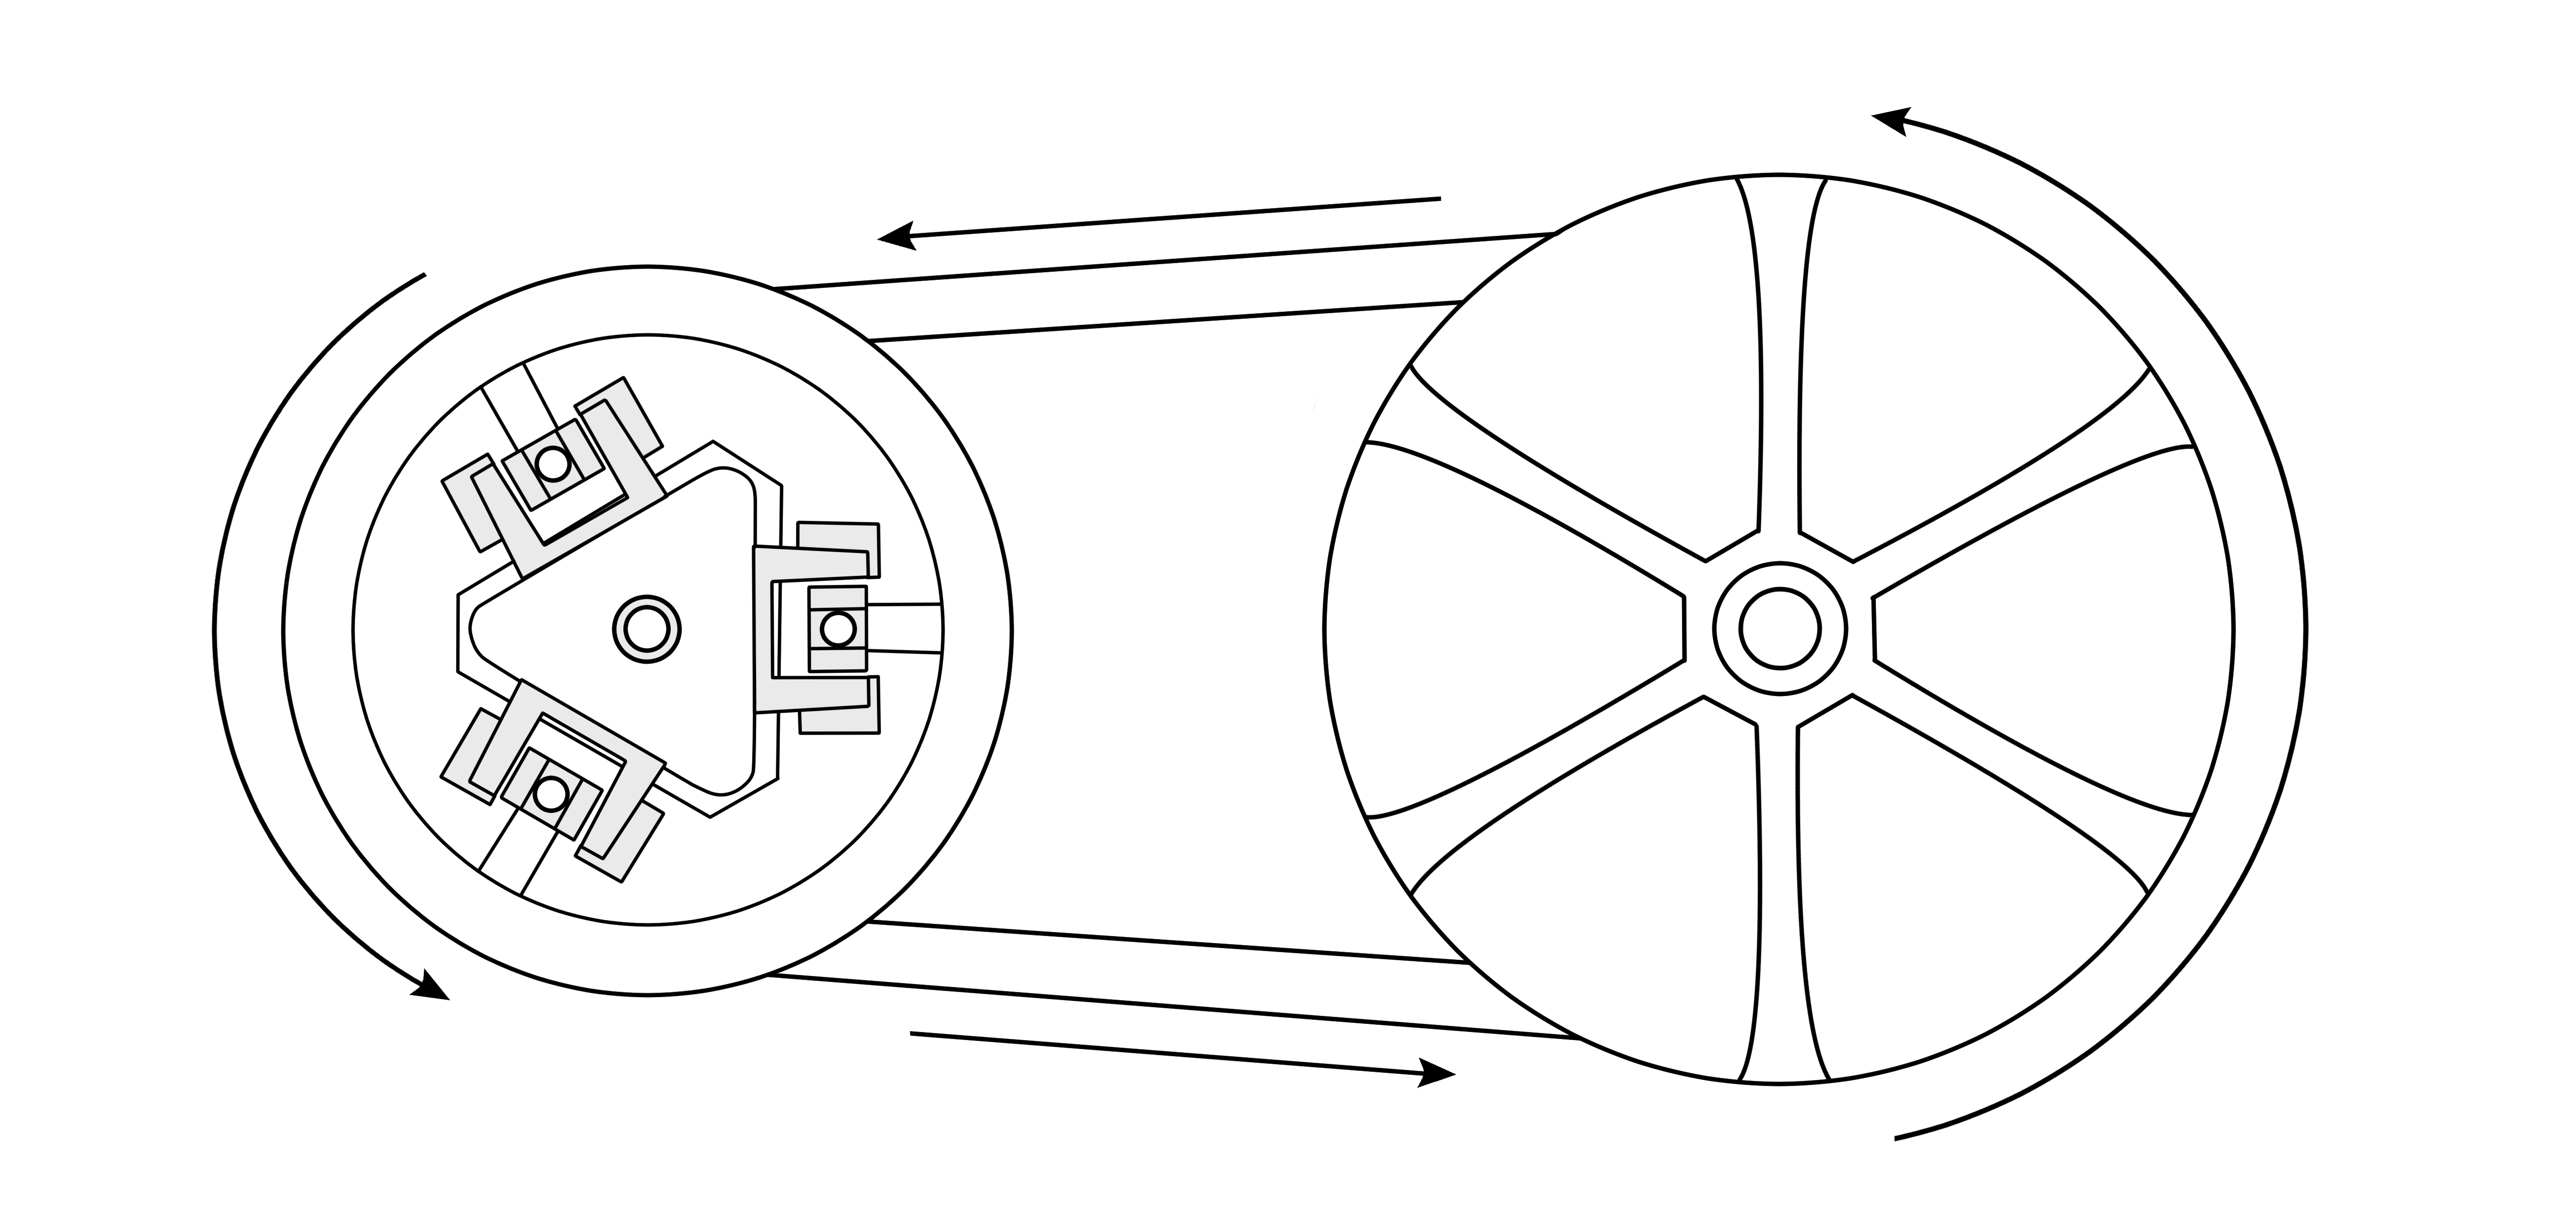
\includegraphics[width=\textwidth]
{figures/coordinate/rotational_direction.png}
\caption{
Rotational and belt-transport sign convention viewed from the outboard pulley
faces, looking inward along the parallel shaft axes. Counterclockwise rotation
is positive for both pulleys. With the primary pulley on the left and the
secondary pulley on the right, positive belt transport runs from secondary to
primary along the upper span and from primary to secondary along the lower
span.
}
\label{fig:rotational_sign}
\end{figure}

Torque follows the corresponding shaft convention. A torque acting on shaft
\(j\in\{p,s\}\) is positive when it acts in the rotational sense defined by
\(\omega_j>0\). In particular, the interface torque
\(\tau_{\mathrm{B},j}>0\) acts on the CVT in this positive direction. The
sign is fixed by the rotational coordinate, not by whether the torque aids or
opposes the shaft's instantaneous motion.

% --------------------------------------------------------------
\subsection{Local Axial Sheave Coordinates}
\label{sec:cvt_axial_direction}

Each movable sheave is assigned a local axial coordinate. Let \(x_p\) denote
the position of the primary movable sheave and \(x_s\) the position of the
secondary movable sheave. More generally, \(x_j\) denotes the corresponding
coordinate for pulley \(j\in\{p,s\}\).

For either pulley, \(x_j=0\) denotes the fully open position. Increasing
\(x_j\) moves the movable sheave toward the fixed sheave and closes the pulley,
while decreasing \(x_j\) opens it. If \(x_{j,\max}\) denotes the available
travel, then

\[
    x_j=0
    \quad\text{is fully open},
    \qquad
    x_j=x_{j,\max}
    \quad\text{is fully closed}.
\]

The velocity follows the same convention:
\(\dot{x}_j>0\) denotes closing motion and
\(\dot{x}_j<0\) denotes opening motion. The fully open position is only the
geometric origin of the coordinate; it does not prescribe the configuration
from which a simulation must begin.

\Cref{fig:cvt_axial_direction} illustrates this convention on the primary
pulley. The secondary uses the same local definition. Because the two
coordinates are local to their respective sheave pairs, their positive
directions may point in opposite physical directions along a common global
axis; in both cases, positive axial motion closes the corresponding pulley.

\begin{figure}[H]
\centering
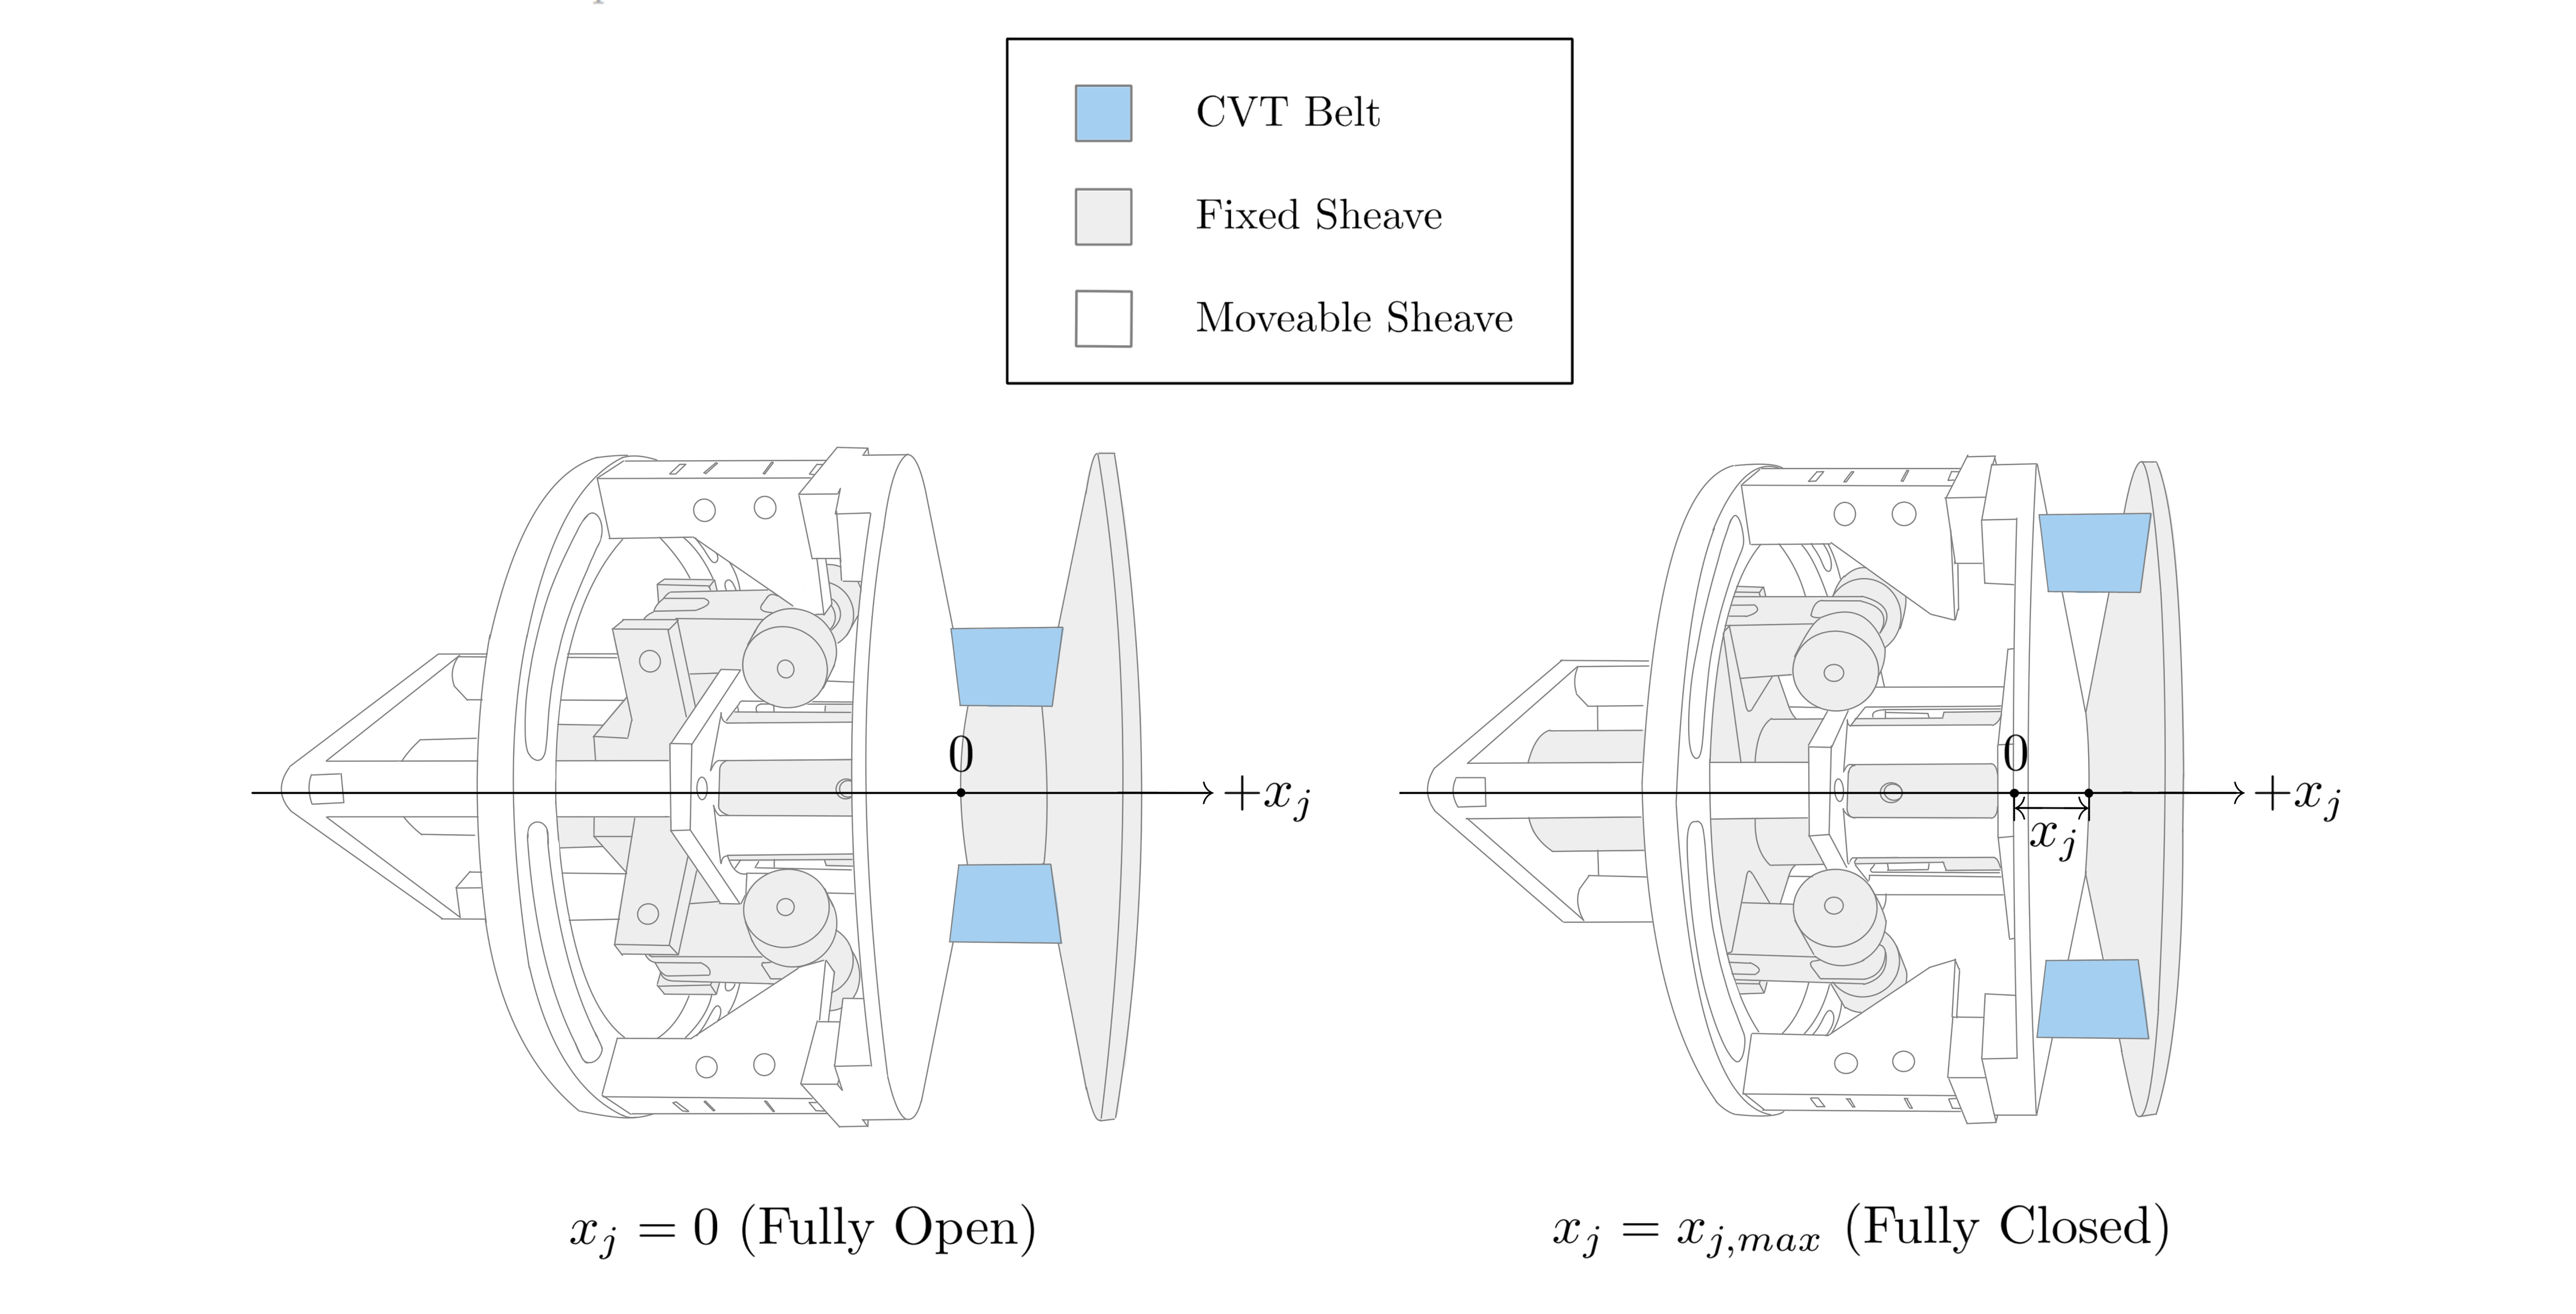
\includegraphics[width=\textwidth]
{figures/coordinate/axial_direction.png}
\caption{
Local axial convention illustrated on the primary movable sheave. \(x_p=0\) 
denotes the fully open position and increasing
\(x_p\) moves the movable sheave toward the fixed sheave. The fully closed
position is \(x_p=x_{p,\max}\). The secondary uses the same local
convention for \(x_s\).
}
\label{fig:cvt_axial_direction}
\end{figure}

% --------------------------------------------------------------
\subsection{Local Radial, Tangential, and Axial Directions}
\label{sec:radial_direction}

At either pulley, the radial and tangential directions lie in the plane of
pulley rotation. At any point around the pulley, the radial unit vector
\(\hat{\mathbf e}_r\) points outward from the pulley axis. The tangential unit
vector \(\hat{\mathbf e}_\theta\) is perpendicular to
\(\hat{\mathbf e}_r\) and points in the direction produced by the positive
rotation defined in \Cref{sec:rotational_sign}. A radial or tangential
component is positive when it points along its corresponding unit vector.

These vectors form a local polar basis rather than a fixed Cartesian pair.
Their directions therefore change with the point around the pulley, while
\(\hat{\mathbf e}_r\) remains outward and \(\hat{\mathbf e}_\theta\) remains
tangent in the positive rotational direction. \Cref{fig:radial_direction}
illustrates this basis on a representative primary pulley; the direction
definitions apply at either pulley. For reference, the axial direction remains
the local closing direction defined in \Cref{sec:cvt_axial_direction}; in the
primary view shown here, positive axial motion points perpendicular to the page 
along the shaft.

\begin{figure}[H]
\centering
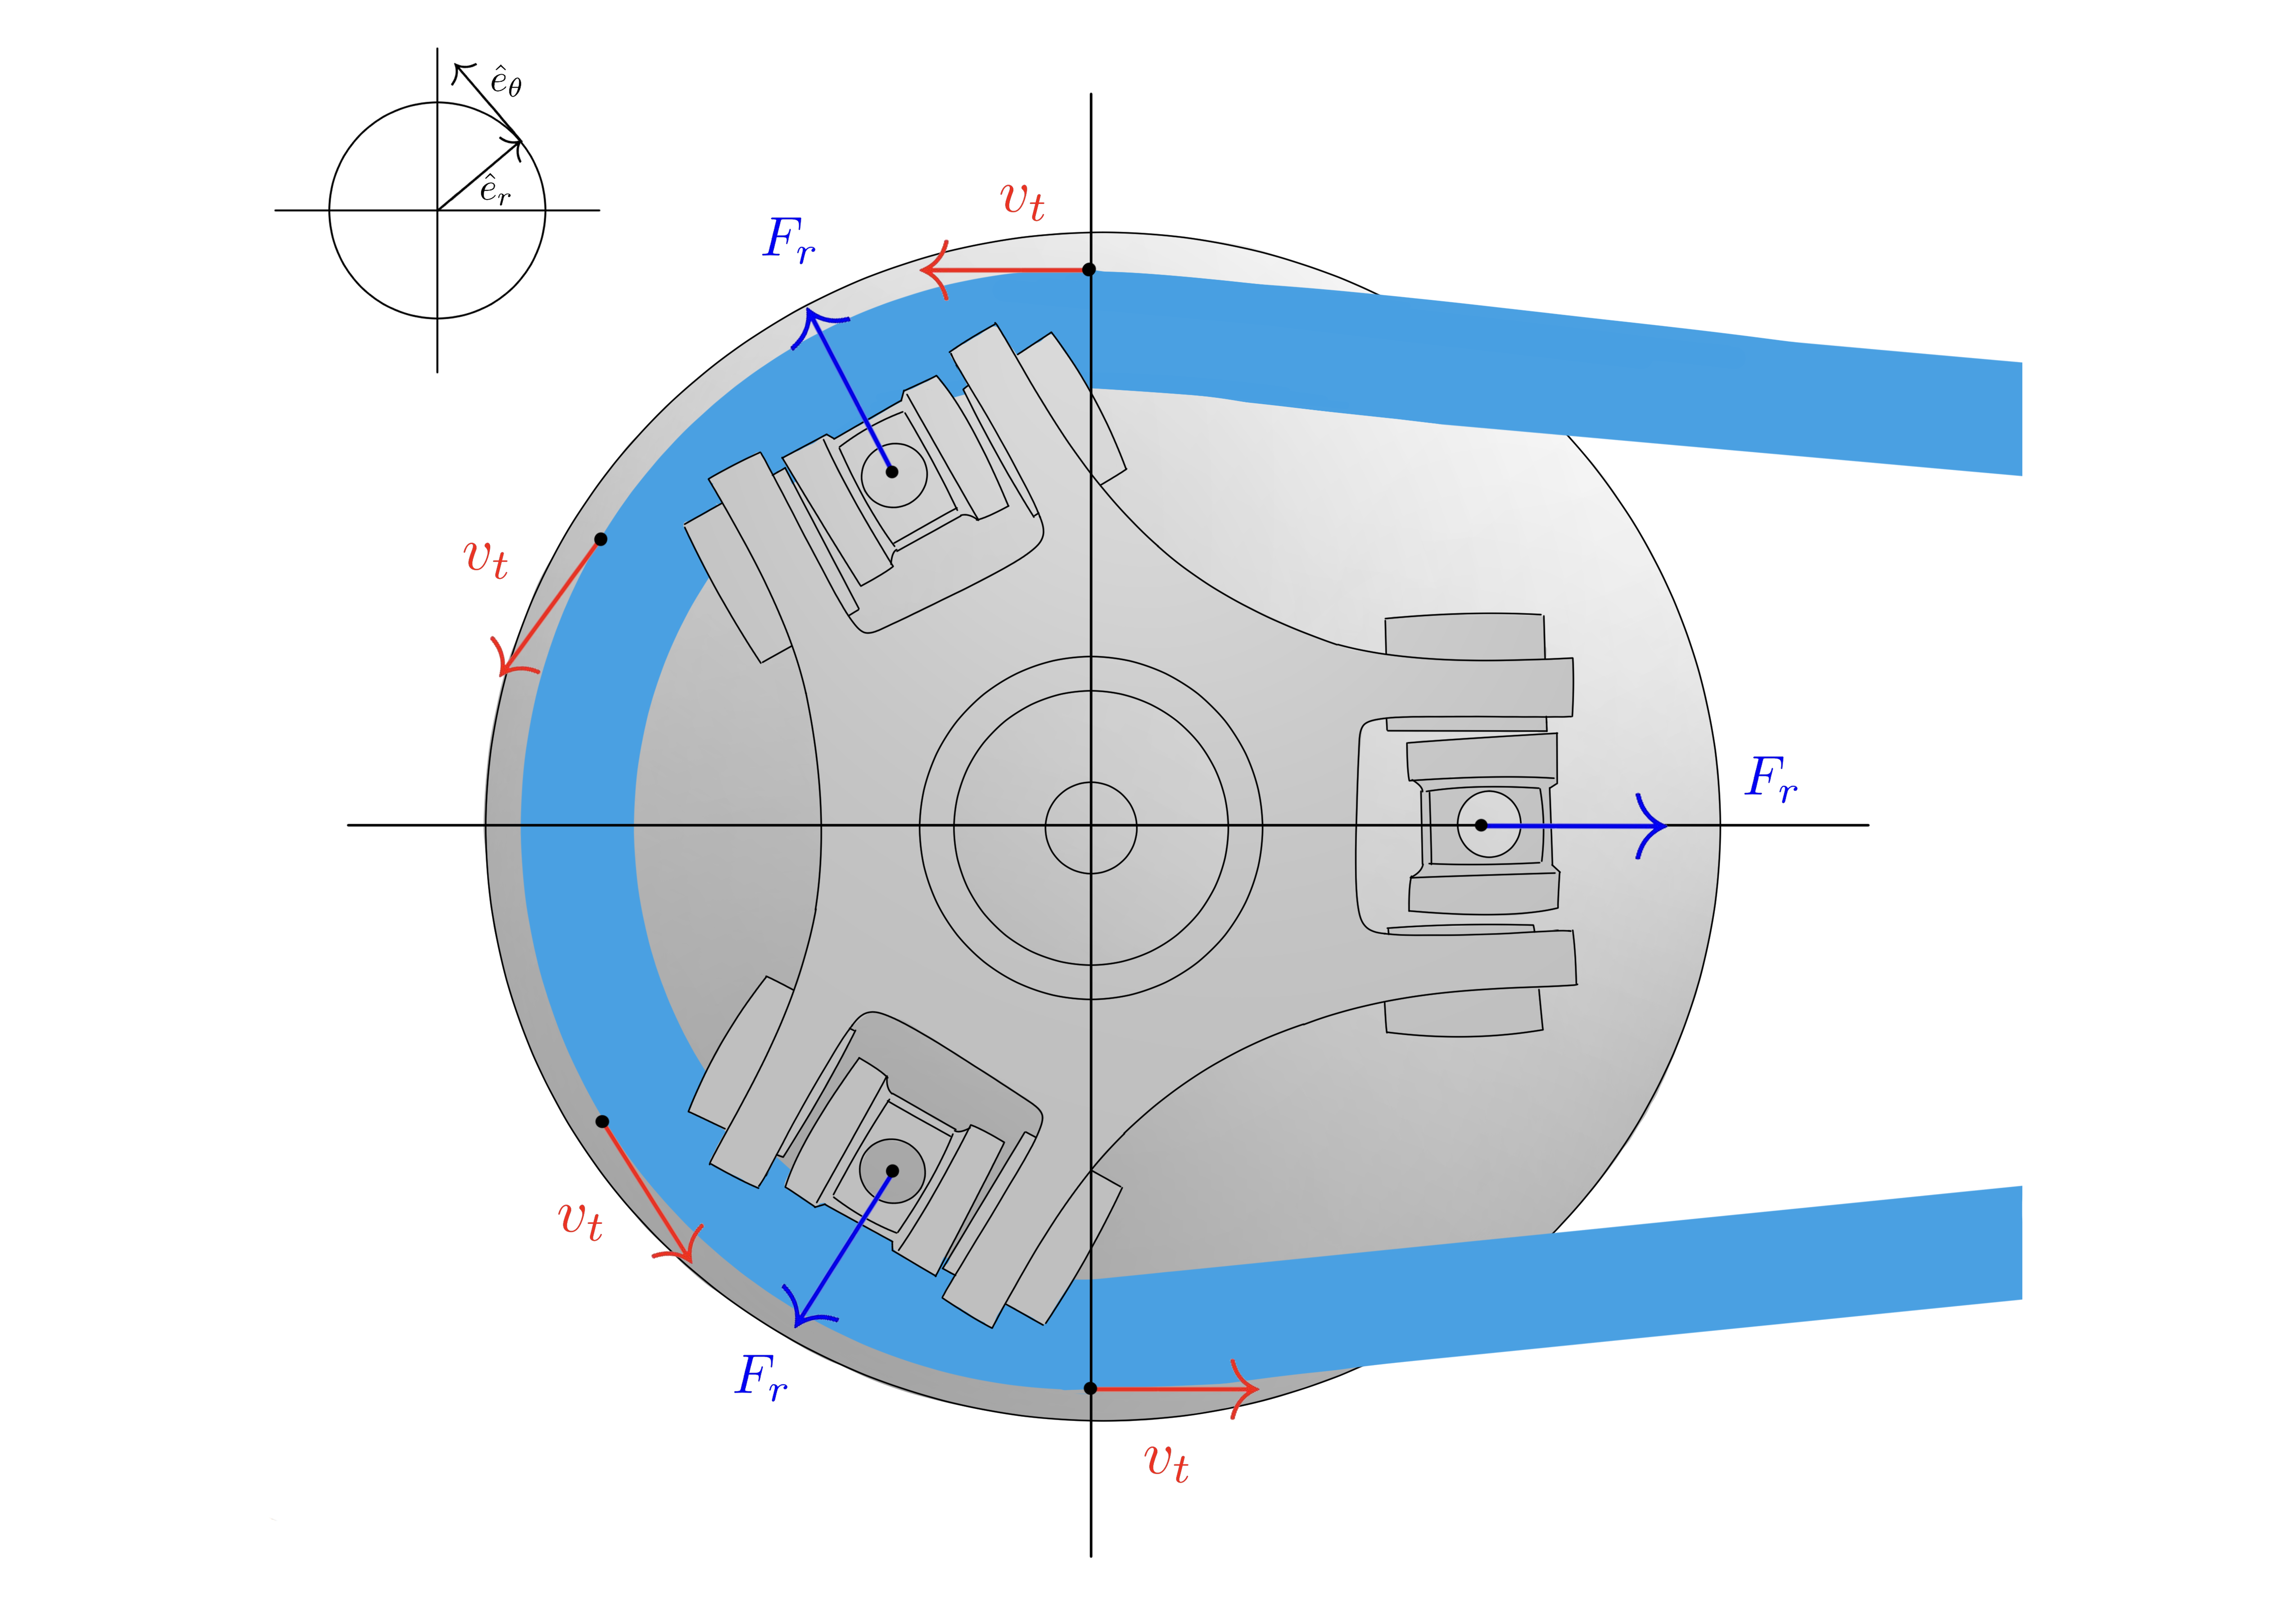
\includegraphics[width=\textwidth]
{figures/coordinate/radial_tangential_direction.png}
\caption{
Representative primary-pulley view of the local radial and tangential
directions. The inset shows the local polar basis:
\(\hat{\mathbf e}_r\) points outward from the pulley axis, while
\(\hat{\mathbf e}_\theta\) is tangent in the positive rotational direction
defined in \Cref{sec:rotational_sign}. The basis changes orientation with the
point around the pulley. All force and velocity arrows
shown are illustrative.
}
\label{fig:radial_direction}
\end{figure}

% ==============================================================

% ==============================================================

\section{CVT State Variables}
\label{sec:continuous_state_variables}

To describe how the CVT evolves, five continuous quantities are carried from 
one instant to the next. They are collected in the state vector,

\bigeq{eq:state-vector}{State Vector}{
\vect{x}(t)=
\begin{bmatrix}
\omega_p \\
\omega_s \\
s \\
\dot{s} \\
v_b
\end{bmatrix}
}

The five entries follow the three retained motions: rotation of the two shafts,
shift of the movable sheaves, and transport of the belt. For the shafts, both
\(\omega_p\) and \(\omega_s\) are retained because the belt couples their
motion without, in general, fixing one speed from the other. No corresponding
shaft-angle states are needed because the retained CVT mechanics do not depend
on the absolute angular orientation of either pulley.

The shift motion requires both a position and a speed. Its position is
represented by \(s\), chosen to increase in the upshift direction. In the
present geometry, this follows closing of the primary movable sheave. Once the
belt is engaged, the fixed belt length and prescribed path of
\AssRef{assump:constant_belt_length} and
\AssRef{assump:prescribed_belt_path} link that primary motion to opening of the
secondary. This gives the physical reason for using one shift coordinate
rather than carrying \(x_p\) and \(x_s\) independently. The exact relation,
including the primary deadzone before engagement, is established later in 
\Cref{sec:pulley_coordinate_mapping}. The corresponding shift speed \(\dot{s}\) 
must also be retained because the moving sheaves and actuation hardware carry inertia. 

The remaining state variable, \(v_b\), describes transport of belt material
around the loop. It is retained independently because tangential slip allows
the belt speed to differ from the surface speed of either pulley. Under
\AssRef{assump:single_belt_speed}, the model carries no separate transport
history for individual belt material points; together with the uniform belt
properties of \AssRef{assump:fixed-belt-cross-section}, this removes the need
for any belt-position coordinate.

Taken together, these five entries are the continuous information carried
forward in time. Their derivative makes clear what must be determined to
advance that state:

\begin{equation}
\dot{\vect{x}}(t)
=
\begin{bmatrix}
\dot{\omega}_p \\
\dot{\omega}_s \\
\dot{s} \\
\ddot{s} \\
\dot{v}_b
\end{bmatrix}.
\label{eq:state-derivative}
\end{equation}

In this derivative, \(\dot{s}\) is already known from the current state. The
mechanics must supply the two shaft accelerations, the shift acceleration, and
the belt-transport acceleration. Once those rates are known, the continuous
state can be advanced to the next instant.

That still does not completely specify how the CVT can evolve. The same values
of \(\vect{x}\) can occur under different contact or support conditions, for
which the allowable motion need not be the same.

\section{Mechanical Regimes and State Evolution}
\label{sec:mechanical_regimes_state_evolution}

As the CVT moves, the contacts and supports that carry load do not remain
fixed. A movable sheave can reach or leave a travel stop, the primary can gain
or lose belt contact, and a belt--pulley interface can change between sticking
and sliding. Each change alters which reactions can exist and which motions the
mechanism can support. The mechanical problem can therefore change even when
the hardware passes through the same positions and velocities.

A travel stop gives the simplest example. Suppose the primary movable sheave is
at the end of its closing travel with \(\dot{s}=0\). If the other forces on the
movable assembly continue to drive it closed, the stop supplies a reaction and
prevents further motion into the boundary. If those forces instead tend to open
the pulley, the stop reaction vanishes and the sheave can accelerate away. The
same continuous state can therefore describe two different mechanical
situations, distinguished by which support is active.

The additional information is the current \emph{mechanical regime}. For the
modeled CVT, the regime records which belt--pulley contacts exist, whether
shift motion is free or held by a mechanical stop, and whether each existing
tangential contact is sticking or sliding. Let \(q(t)\) denote the current
regime. This label is not another mechanical coordinate; it is a compact
description of the active mechanical arrangement.

Together, \(\vect{x}(t)\) and \(q(t)\) describe the internal CVT condition
carried from one instant to the next. While one regime persists, the same
contacts, supports, and kinematic restrictions remain active, so the state
follows one continuous set of mechanical balances. Within that regime, the 
continuous mechanics must relate the current state and shaft loading to the 
state derivative. This dependence can be represented schematically as

\begin{equation}
\dot{\vect{x}}
=
\mathcal{F}_{q}
\!\left(
    t,\vect{x},
    \tau_{\mathrm{B},p},I_{\mathrm{B},p},
    \tau_{\mathrm{B},s},I_{\mathrm{B},s}
\right).
\label{eq:regime_dependent_evolution}
\end{equation}

Here, \(\mathcal{F}_{q}\) is only a compact representation of the continuous
mechanics. Its subscript records that changing the active arrangement changes
which balances and constraints apply. As long as the conditions defining the
regime remain satisfied, \(q\) is unchanged and the state evolves
continuously.

A regime persists only while those physical conditions can be maintained. As
the CVT moves, a stop may be reached or released, belt contact may form or
separate, or a tangential contact may reach the boundary between sticking and
sliding. Such an event changes the active mechanical arrangement. Whether the
state itself changes at that instant depends on what changed physically.

If a stop releases from rest, or another contact condition changes without
producing an impulse, the configuration and velocities pass through the event
unchanged,

\begin{equation}
    \vect{x}^{+}=\vect{x}^{-},
    \label{eq:nonimpulsive_regime_transition}
\end{equation}

where the superscripts \(-\) and \(+\) denote values immediately before and
after the event. The state is continuous, but its derivative can change
immediately because the new regime applies a different set of balances and
constraints.

A different situation occurs when a new rigid kinematic constraint becomes
active while the mechanism still has finite velocity into it. The incoming
motion may then be incompatible with the motion allowed after the constraint
forms. Under \AssRef{assump:inelastic_constraint_activation}, the activation is
treated as instantaneous and perfectly inelastic. The CVT does not jump to a 
new shift position during that instant, but its retained velocities may change 
to satisfy the newly active constraint. Thus,

\begin{equation}
    s^{+}=s^{-},
    \qquad
    \begin{bmatrix}
        \omega_p^{+}\\
        \omega_s^{+}\\
        \dot{s}^{+}\\
        v_b^{+}
    \end{bmatrix}
    \;\text{need not equal}\;
    \begin{bmatrix}
        \omega_p^{-}\\
        \omega_s^{-}\\
        \dot{s}^{-}\\
        v_b^{-}
    \end{bmatrix}.
    \label{eq:impulsive_regime_transition}
\end{equation}

Once a compatible post-event motion has been established, continuous evolution 
resumes under the new regime.

The CVT motion therefore consists of continuous intervals under a fixed regime
connected by discrete changes in the active mechanical arrangement. Because
both forms of evolution are part of the same problem, the model forms a
\emph{hybrid initial-value problem}. A complete initial condition specifies an
initial state together with an admissible initial regime,

\begin{equation}
    \vect{x}(t_0)=\vect{x}_0,
    \qquad
    q(t_0)=q_0,
    \label{eq:hybrid_initial_condition}
\end{equation}

with \(\vect{x}_0\) satisfying the contacts and constraints represented by
\(q_0\). The regimes are not separate CVT models. They are different
admissible arrangements of the same pulley assemblies, belt, actuation
mechanisms, and shaft interfaces. The state vector records how that mechanism
is moving; the regime records which motion is presently allowed.

\section{Model Quantities and Evaluation Flow}
\label{sec:model_evaluation_flow}

One CVT model evaluation brings together quantities that do not all play the
same role. Some define the particular CVT being modeled, some describe its
current internal condition, some enter through the two shaft interfaces, and
some are determined only after the current mechanics are evaluated. Keeping
these roles separate makes clear what is fixed, what is carried forward, what
is supplied from outside the CVT, and what must be found again at the current
instant.

The fixed CVT data are the physical and geometric quantities that define the
selected hardware. Some may be specified directly and others calculated once
from those inputs during initialization; in either case, they remain unchanged
while that simulation is advanced. \Cref{tab:model_quantity_roles} places these
data alongside the three roles that can change from one evaluation to the next.

\begin{table}[H]
\centering
\renewcommand{\arraystretch}{1.12}
\caption{Roles of the quantities used during a CVT model evaluation.}
\label{tab:model_quantity_roles}
\begin{tabular}{
>{\raggedright\arraybackslash}p{0.16\linewidth}
>{\raggedright\arraybackslash}p{0.22\linewidth}
>{\raggedright\arraybackslash}p{0.36\linewidth}
>{\raggedright\arraybackslash}p{0.14\linewidth}}
\toprule
\textbf{Quantity role}
& \textbf{Contents}
& \textbf{Use during evaluation}
& \textbf{Inventory} \\
\midrule
Fixed CVT data
& Physical and geometric data for the selected hardware, including values
  calculated once during initialization
& Define the selected CVT and the mechanical relations used to represent it;
  remain unchanged during one simulation.
& \Cref{tab:cvt_fixed_data} \\
\addlinespace[3pt]

Current CVT condition
& State vector \(\vect{x}(t)\) and mechanical regime \(q(t)\)
& Carry the current internal motion and active mechanical arrangement from the
  preceding instant.
& \Cref{tab:cvt_current_condition} \\
\addlinespace[3pt]

Shaft-interface conditions
& Applied torque \(\tau_{\mathrm{B},j}\) and equivalent inertia
  \(I_{\mathrm{B},j}\) at each shaft
& Supply the current mechanical loading presented by the systems attached to
  the primary and secondary shafts.
& \Cref{tab:cvt_shaft_interface_conditions} \\
\addlinespace[3pt]

Instantaneous CVT quantities
& State derivative \(\dot{\vect{x}}(t)\) and other mechanical quantities
  required for the current evaluation, including regime-admissibility measures
& Are determined from the fixed CVT data, current CVT condition, and
  shaft-interface conditions; determine how the state can advance and whether
  the current regime can continue.
& \Cref{tab:cvt_instantaneous_quantities} \\
\bottomrule
\end{tabular}
\end{table}

Taken together, these roles separate what defines an instantaneous CVT problem
from what the mechanics return. The fixed data identify the hardware, the
shaft-interface conditions provide its current external loading, and
\(\bigl(\vect{x},q\bigr)\) gives the internal condition to which that loading
is applied. The instantaneous quantities are the response of that condition.
One evaluation can therefore be stated compactly:

\begin{enumerate}
    \item The current time, state \(\vect{x}(t)\), and regime \(q(t)\) identify
          the internal CVT condition at the start of the evaluation.
    \item The systems attached to the primary and secondary shafts supply the
          torque and equivalent inertia presented at their respective
          interfaces under the current shaft conditions.
    \item The CVT mechanics use the fixed CVT data, current internal condition,
          and shaft-interface conditions to determine the instantaneous
          mechanical response. This provides \(\dot{\vect{x}}(t)\) together
          with the quantities needed to test whether the current regime remains
          admissible.
    \item If the regime remains admissible, the state is advanced using
          \(\dot{\vect{x}}\) and the regime is retained. If an event changes
          the active mechanical arrangement, any required finite-speed
          transition establishes a compatible post-event state before
          continuous evolution resumes under the resulting regime.
    \item The resulting state and regime become the current internal condition
          for the next evaluation, and the cycle repeats.
\end{enumerate}

The information required to pose each instantaneous CVT problem is now
defined. What remains is the mechanical response itself: the coupled forces,
torques, and accelerations implied by the current geometry, actuation, belt
motion, and contact state.

\chapter{Derivation}
\label{chap:derivation}

\Cref{chap:model_setup} established the CVT as a hybrid initial-value problem: at a given
instant, the current state, mechanical regime, and shaft-interface loading are
known, and the model must determine the corresponding instantaneous response.
This chapter derives the mechanics required to perform that evaluation. The
development begins with the most general continuous configuration, in which the
belt is fully engaged and the CVT is free to shift, and then returns to the
mechanical boundaries and regime changes that connect successive intervals of
continuous motion.

\Cref{sec:geometry} first develops the pulley and belt-loop kinematics, reducing
the motion of both sheaves and both pulley radii to the shared shift coordinate.
Using that kinematic structure, \Cref{sec:axial_actuation_balances} derives the
axial actuation and movable-sheave dynamics, while
\Cref{sec:pulley_rotational_dynamics} develops the corresponding rotational
dynamics of the two pulley assemblies. \Cref{sec:belt_transport_contact} then
closes the mechanics of the belt itself, relating its transport motion,
tension, pulley loading, and transmitted torque. These pieces are assembled in
\Cref{sec:engaged_dynamic_closure}, where the admissible belt--pulley contact
state completes the instantaneous dynamics of the freely shifting engaged CVT.
\Cref{sec:shift_regime_dynamics} then extends this result to the remaining
mechanical regimes, showing how the continuous equations reduce when additional
constraints become active and how the state is carried consistently through
transitions between them. Finally, \Cref{sec:complete_system_evaluation}
brings these results together in the complete-system evaluation outlined in
\Cref{sec:model_evaluation_flow}, showing how the CVT can be followed through
time.

\section{Pulley Geometry}
\label{sec:geometry}

The conceptual overview introduced the CVT as two variable-radius pulleys
connected by a single belt. Moving the pulley sheaves changes where the belt
sits on each pulley and therefore changes the transmission ratio.

Both pulleys contain a movable sheave. Let \(x_p\) denote the axial position of
the movable primary sheave and \(x_s\) the axial position of the movable
secondary sheave. The geometric problem is therefore twofold: how does the
axial position of each movable sheave set the belt radius on its own pulley,
and how does the shared belt constrain the two pulley positions to move
together?

The first question can be answered from the local geometry of each pulley.
The second requires following the belt around the complete loop. Once these
position relationships are known, they can be differentiated to obtain the
corresponding radius rates and accelerations.

The natural place to begin is the geometry of a single pulley.

\subsection{Local Pulley Geometry}
\label{sec:local_pulley_geometry}

The first part of the geometric question can be answered on a single pulley:
how does the axial position of its movable sheave determine the pulley radius?
The same conical geometry appears on both pulleys, so the relationship can be
derived once and then applied to the primary and secondary.

The axial direction and primary-sheave convention were introduced in
\Cref{sec:cvt_axial_direction} and illustrated in
\Fig{fig:cvt_axial_direction}. The local coordinates \(x_p\) and \(x_s\)
follow the same convention on their respective pulleys.

For either pulley \(j\in\{p,s\}\), \(x_j=0\) denotes the fully open
configuration. Increasing \(x_j\) moves the movable sheave toward the fixed
sheave and closes the pulley, while decreasing \(x_j\) opens it. The
corresponding velocity follows the same sign convention:
\(\dot{x}_j>0\) denotes closing motion and \(\dot{x}_j<0\) denotes opening
motion.

The primary therefore begins at \(x_p=0\) and moves in the positive direction
as it closes. The secondary begins in a closed position, with \(x_s>0\), and
moves toward smaller values of \(x_s\) as it opens.

Consider a belt seated between two straight sheave faces with half-angle
\(\beta\), as shown in \Cref{fig:local_pulley_geometry}. Let
\(b_{\mathrm{in}}\) denote the width of the belt at its inner surface. As
assumed in \AssRef{assump:fixed-belt-cross-section}, this width remains constant.

Suppose the movable sheave closes the pulley by a distance \(\Delta x_j\).
At the original belt radius, the available space between the sheaves is
therefore reduced from \(b_{\mathrm{in}}\) to

\[
b_{\mathrm{in}}-\Delta x_j.
\]

The belt responds by moving outward through a radial distance
\(\Delta r_j\). At its new position, the angled sheave faces provide an
additional axial distance \(d\) on each side.

\begin{figure}[H]
\centering
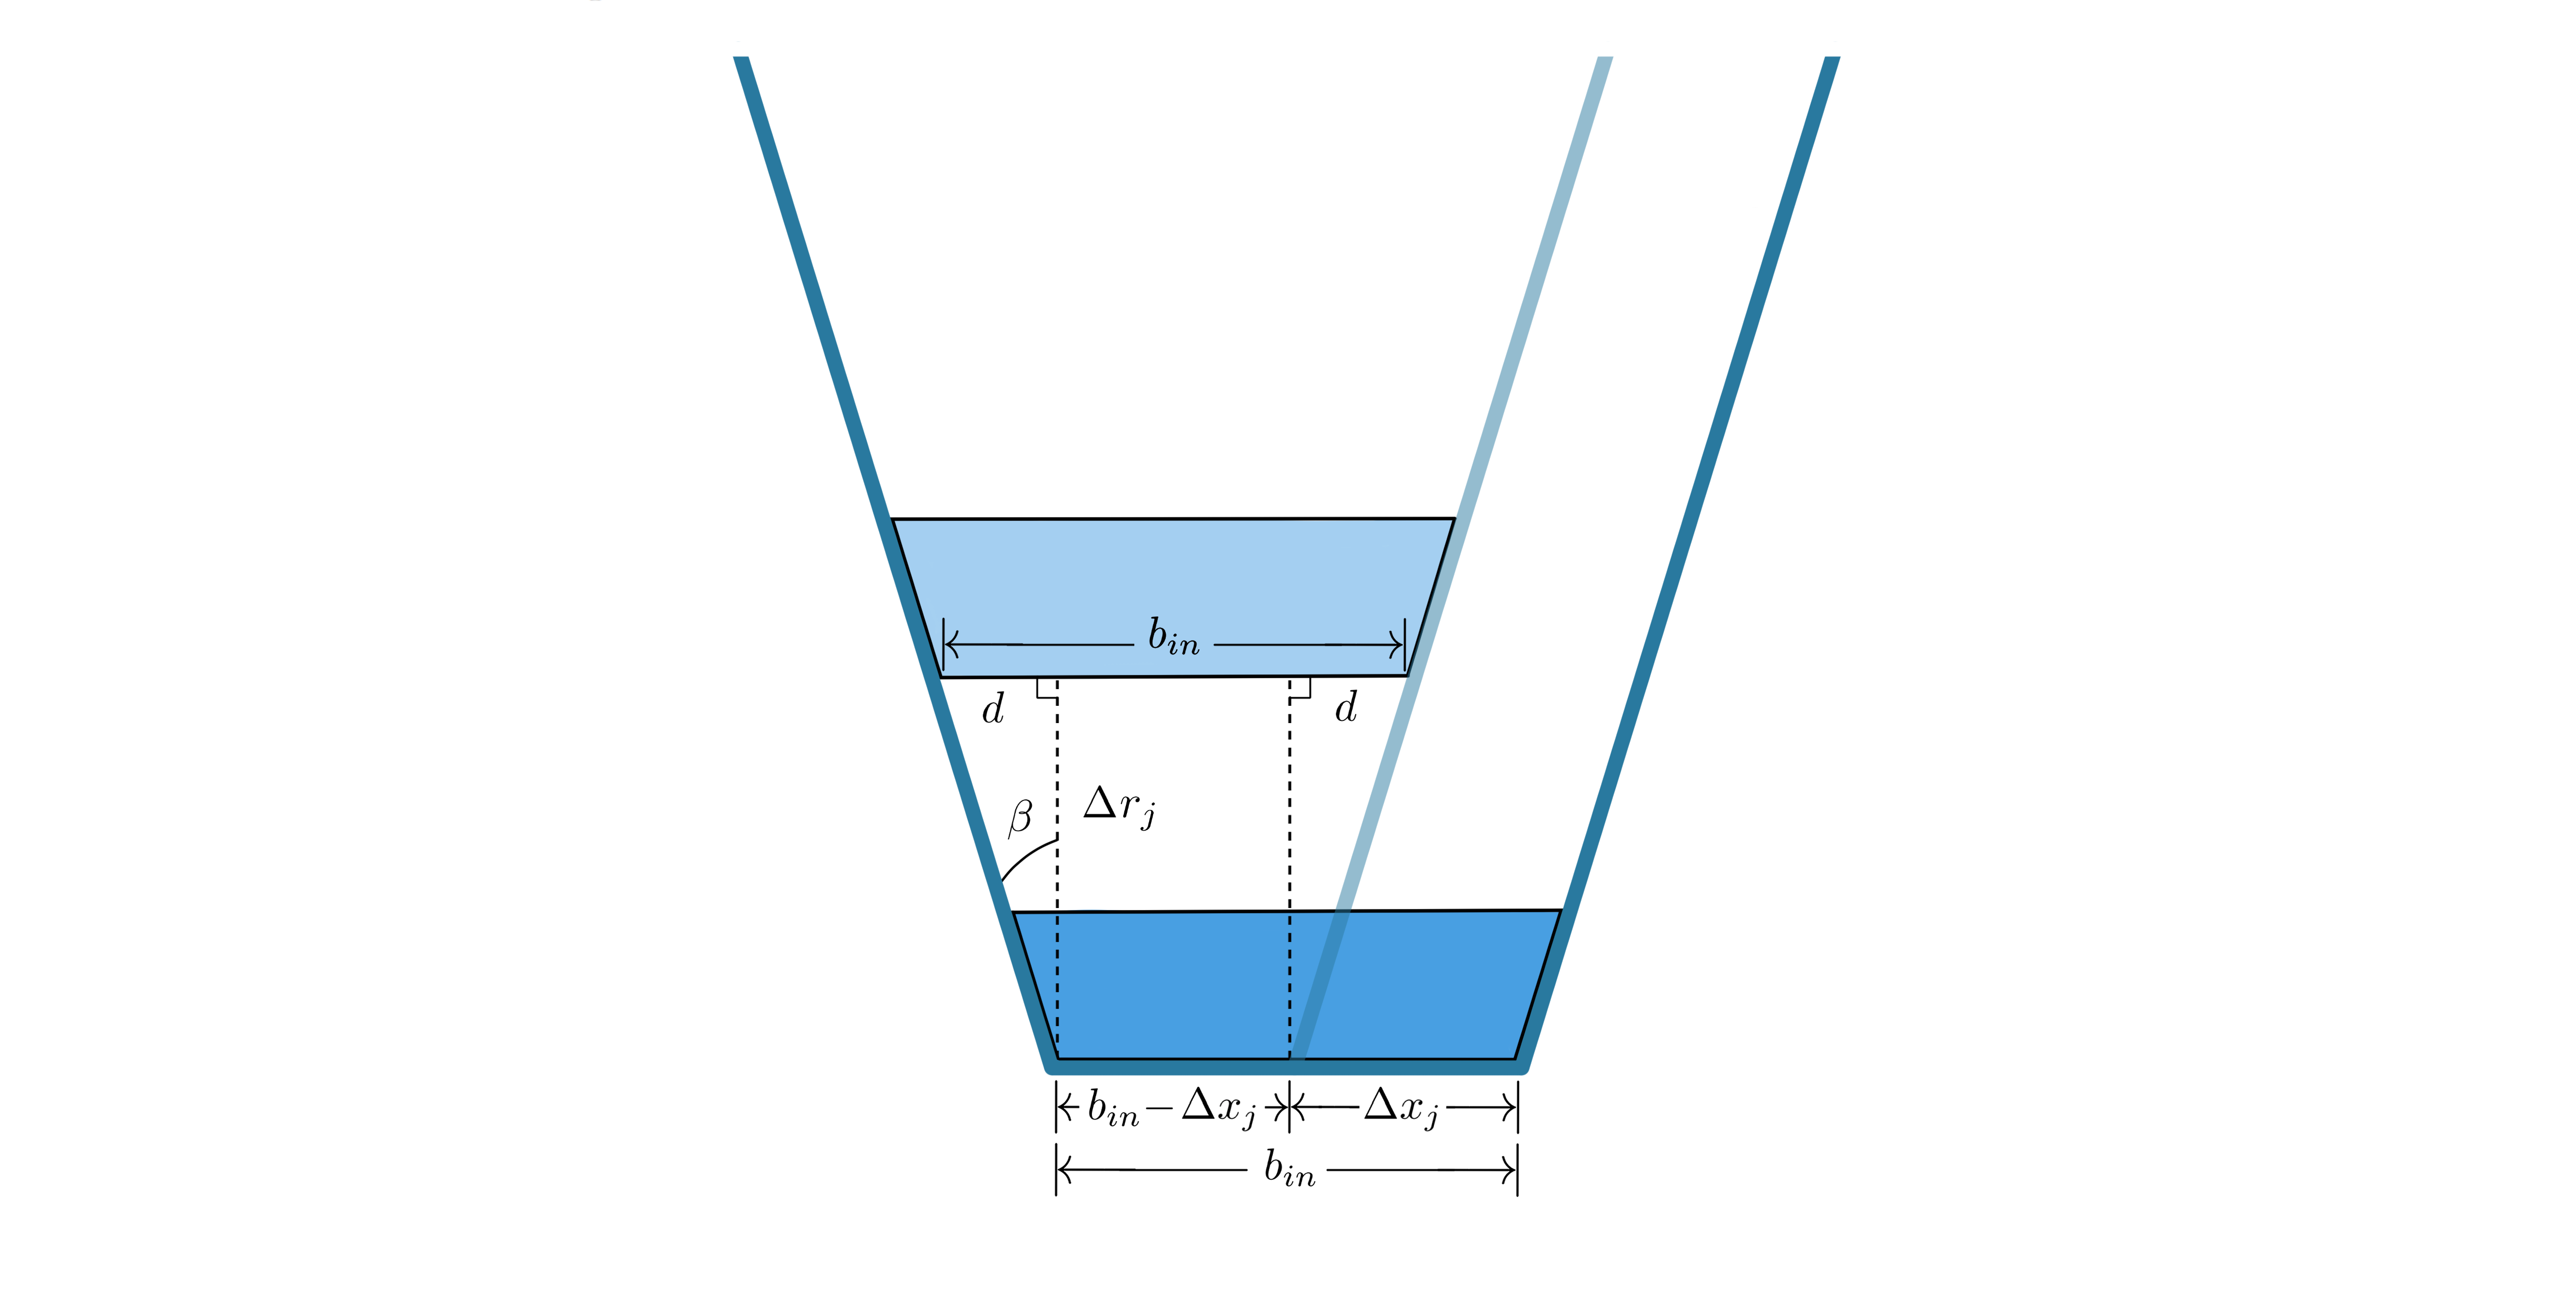
\includegraphics[width=\linewidth]{figures/geometry/local_pulley_geometry.png}
\caption{
Local geometry of a belt moving outward between the sheave faces of pulley
\(j\). Closing the pulley by \(\Delta x\) reduces the available width at
the original belt position to \(b_{\mathrm{in}}-\Delta x\). Moving outward
by \(\Delta r\) provides an additional axial distance \(d\) at each
sheave face.
}
\label{fig:local_pulley_geometry}
\end{figure}

At the new radius, the total space between the sheave faces must again equal
the fixed belt width. Reading directly from
\Cref{fig:local_pulley_geometry},

\begin{equation}
b_{\mathrm{in}}
=
2d+\left(b_{\mathrm{in}}-\Delta x_j\right).
\label{eq:local_width_balance}
\end{equation}

The right triangle beside either sheave face relates \(d\) to the radial
movement. For the sheave half-angle \(\beta\),

\begin{equation}
\tan\beta
=
\frac{d}{\Delta r_j},
\end{equation}

and therefore

\begin{equation}
d
=
\Delta r_j\tan\beta.
\label{eq:local_triangle_distance}
\end{equation}

Substituting \Cref{eq:local_triangle_distance} into
\Cref{eq:local_width_balance} gives

\begin{equation}
b_{\mathrm{in}}
=
2\Delta r_j\tan\beta
+
\left(b_{\mathrm{in}}-\Delta x_j\right).
\end{equation}

The constant belt-width terms cancel, leaving

\begin{equation}
\Delta r_j
=
\frac{\Delta x_j}{2\tan\beta}.
\label{eq:local_cone_geometry}
\end{equation}

This is the basic axial-to-radial relationship of the pulley. Closing the
pulley moves the belt outward, while opening it moves the belt inward. A
smaller sheave angle produces more radial movement for the same axial motion,
whereas a larger sheave angle produces less.

Taking the infinitesimal limit of
\Cref{eq:local_cone_geometry} gives

\begin{equation}
\frac{dr_j}{dx_j}
=
\frac{1}{2\tan\beta}.
\label{eq:local_radius_position_derivative}
\end{equation}

Because the sheave faces are straight, this slope is constant.

\paragraph{Radius convention}

The derivation above follows the inner surface of the belt, where
\(b_{\mathrm{in}}\) is defined. The belt also has the finite radial height
\(h_b\), so its inner and outer surfaces occupy different radii. Let
\(r_{j,\mathrm{inner}}\) and \(r_{j,\mathrm{outer}}\) denote those radii.
They are related by

\begin{equation}
r_{j,\mathrm{outer}}
=
r_{j,\mathrm{inner}}+h_b.
\label{eq:inner_outer_radius_relation}
\end{equation}

The fixed-cross-section assumption in
\AssRef{assump:fixed-belt-cross-section} makes \(h_b\) constant, so the
axial-to-radial displacement derived above can be read from either surface.
An absolute pulley radius must nevertheless identify which surface is being
measured. The outer surface is used here because it provides a convenient and
directly measurable reference. Throughout the geometric development,

\begin{equation}
r_j
\equiv
r_{j,\mathrm{outer}}.
\label{eq:geometry_radius_convention}
\end{equation}

Using the outer surface gives a clear measure of where the belt is seated. It
does not mean that every physical property of the belt acts at that radius.

The belt tension is carried along the cords embedded within the belt, so it
acts through the centre of the cord layer. The distance from the pulley shaft
to this line is therefore the lever arm through which belt tension transmits
torque, making it the effective radius for gearing. This cord-line radius is
commonly called the pitch radius \citep{Gerbert1996}.

Let \(d_{\mathrm{cord}}\) denote the radial depth of the cord-layer centre from
the outer surface, with \(0<d_{\mathrm{cord}}<h_b\). Because the cord line
lies this far inside the outer surface, its effective radius is

\begin{equation}
r_{j,\mathrm{eff}}
=
r_{j,\mathrm{outer}}-d_{\mathrm{cord}}.
\label{eq:local_belt_effective_radius}
\end{equation}

The belt mass is spread throughout the whole cross-section rather than
concentrated at the outer surface or the cord line. To describe where this
mass is with one radius, we use its centre of mass and denote the radius to
that point by \(r_{j,\mathrm{cm}}\). Under the uniform-density approximation,
the centre of mass is the geometric centroid of the trapezoid.

Let \(y\) measure radially inward from the outer surface, with \(y=0\) at the
outer surface and \(y=h_b\) at the inner surface, and let
\(y_{\mathrm{cm}}\) denote the depth of the centre of mass. These two depths
and their corresponding radii are shown in
\Cref{fig:belt_cross_section_radial_references}.

\begin{figure}[H]
\centering
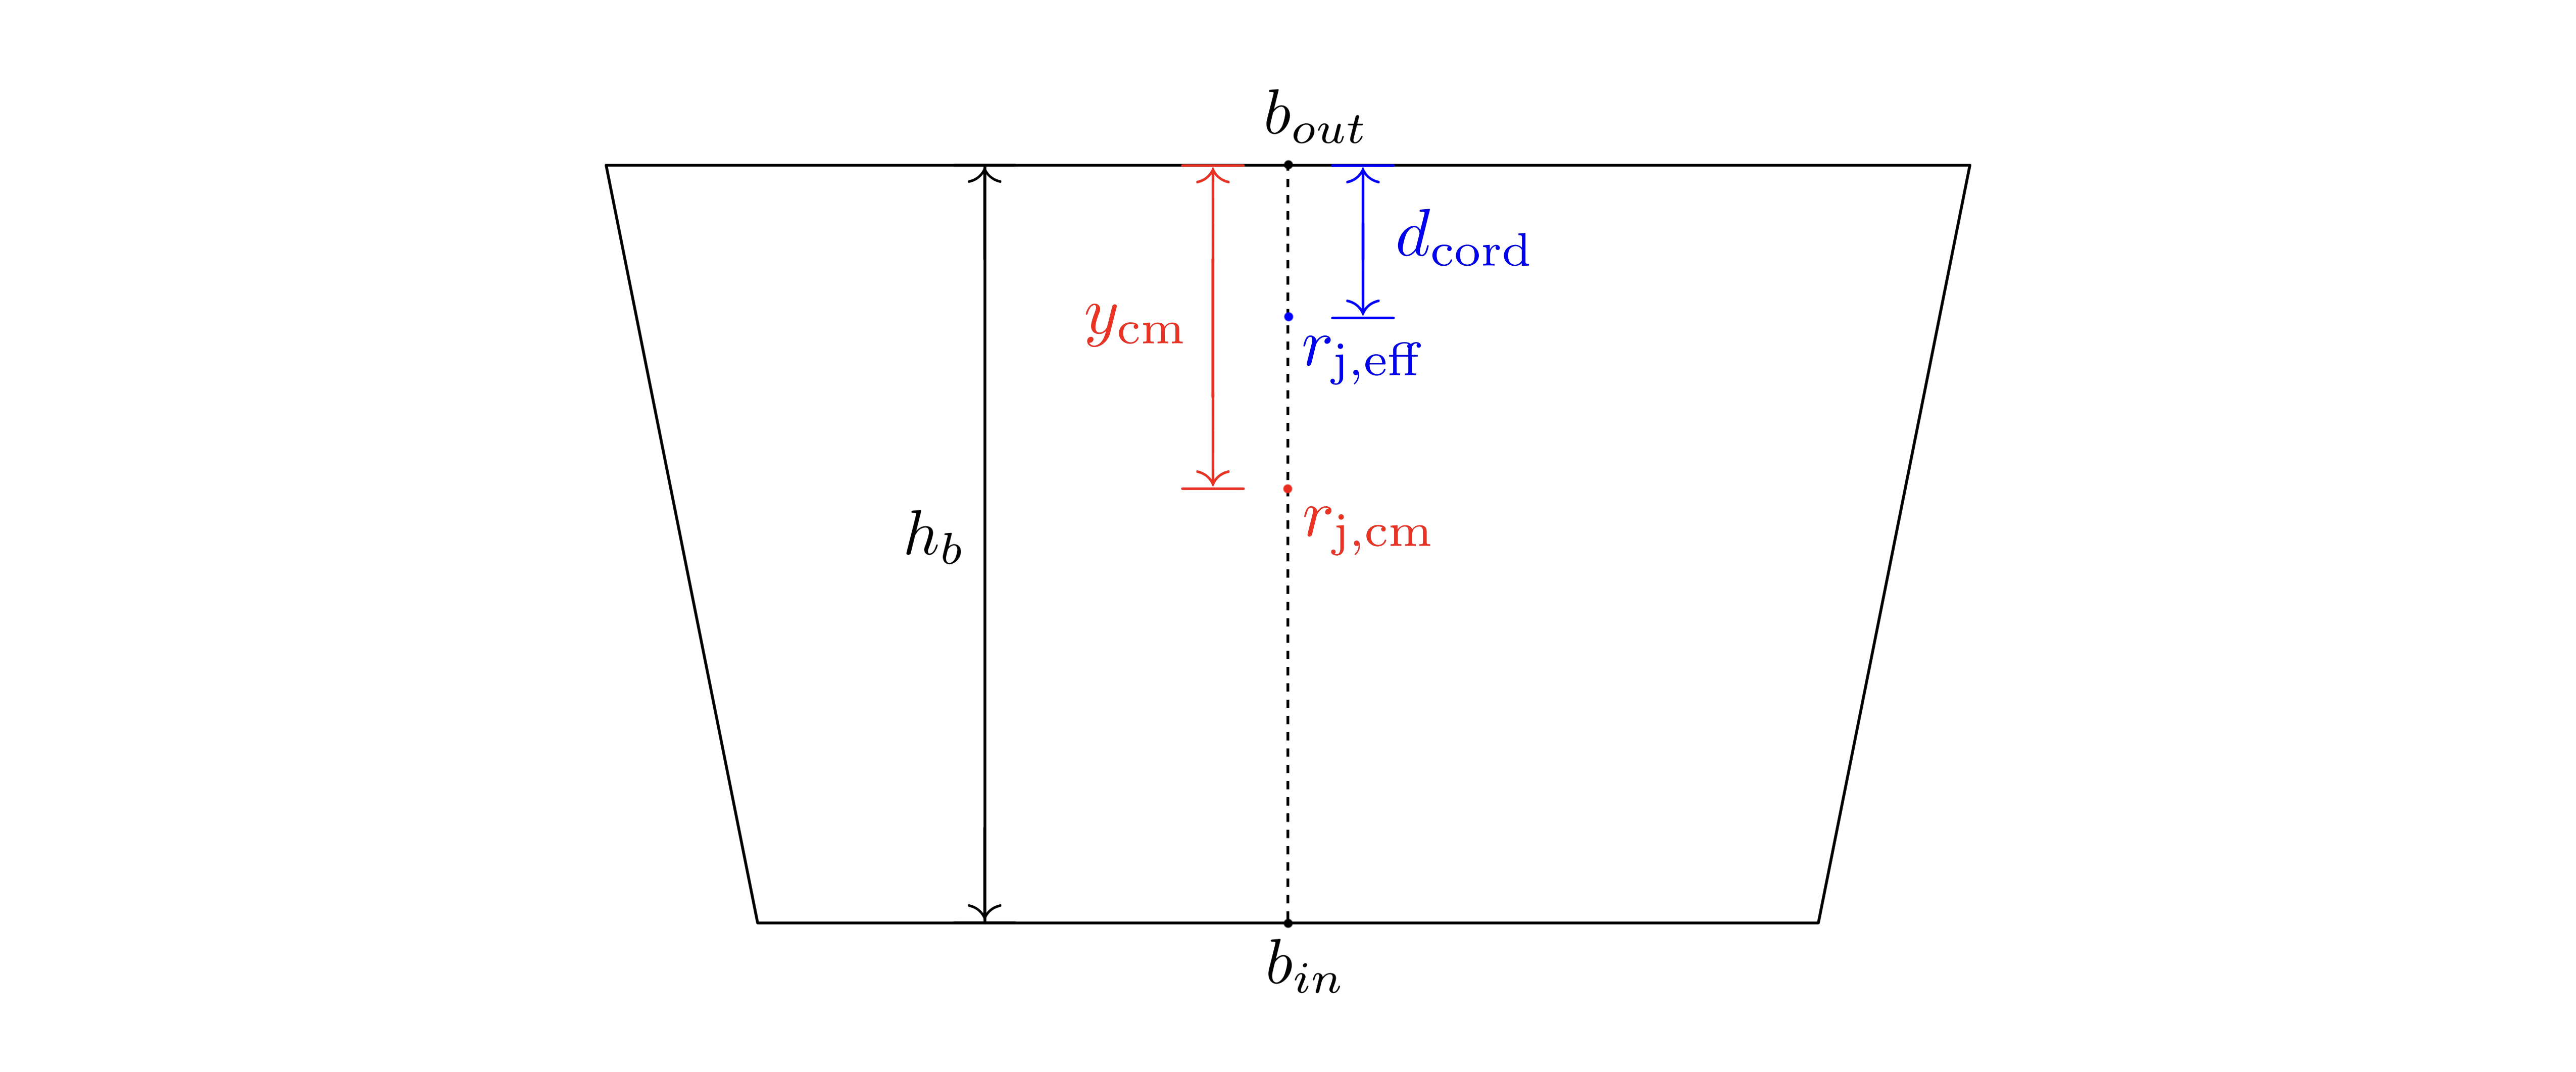
\includegraphics[width=\linewidth]
{figures/geometry/belt_cross_section_radial_references.png}
\caption{
Radial reference lines within the belt cross-section. The cord-line radius
\(r_{j,\mathrm{eff}}\) is the lever arm through which belt tension transmits
torque, while \(r_{j,\mathrm{cm}}\) locates the belt's centre of mass. The
depths \(d_{\mathrm{cord}}\) and \(y_{\mathrm{cm}}\) are measured radially
inward from the outer surface.
}
\label{fig:belt_cross_section_radial_references}
\end{figure}

If \(b_{\mathrm{out}}\) and \(b_{\mathrm{in}}\) are the outer and inner
widths, respectively, the straight sides of the trapezoid give

\begin{equation}
b(y)
=
b_{\mathrm{out}}
-
\frac{b_{\mathrm{out}}-b_{\mathrm{in}}}{h_b}\,y.
\label{eq:local_belt_cross_section_width_distribution}
\end{equation}

Because the density is uniform, a thin strip at depth \(y\) contains mass in
proportion to its area \(b(y)\,dy\). The centroid depth is therefore the
weighted average of \(y\) over the cross-section:

\begin{equation}
y_{\mathrm{cm}}
=
\frac{
    \displaystyle\int_0^{h_b} y\,b(y)\,dy
}{
    \displaystyle\int_0^{h_b} b(y)\,dy
}.
\label{eq:local_belt_cross_section_centroid_definition}
\end{equation}

The denominator is the belt cross-sectional area,

\begin{equation}
A_b
=
\int_0^{h_b} b(y)\,dy
=
\frac{h_b}{2}
\left(b_{\mathrm{out}}+b_{\mathrm{in}}\right).
\label{eq:local_belt_cross_section_area}
\end{equation}

Using this area in the weighted average gives

\begin{equation}
\begin{aligned}
y_{\mathrm{cm}}
&=
\frac{1}{A_b}
\int_0^{h_b} y\,b(y)\,dy
\\[4pt]
&=
h_b
\frac{b_{\mathrm{out}}+2b_{\mathrm{in}}}
{3\left(b_{\mathrm{out}}+b_{\mathrm{in}}\right)}.
\end{aligned}
\label{eq:local_belt_cross_section_centroid}
\end{equation}

The result has the expected limiting behaviour. If
\(b_{\mathrm{out}}=b_{\mathrm{in}}\), the cross-section is rectangular and
\(y_{\mathrm{cm}}=h_b/2\). For the usual trapezoid with
\(b_{\mathrm{out}}>b_{\mathrm{in}}\), the additional area near the outer
surface places the centroid slightly closer to that surface, so
\(y_{\mathrm{cm}}<h_b/2\). The belt mass therefore follows the radius

\begin{equation}
r_{j,\mathrm{cm}}
=
r_{j,\mathrm{outer}}-y_{\mathrm{cm}}.
\label{eq:local_belt_mass_centroid_radius}
\end{equation}

The outer-surface radius map still requires one known configuration to
establish its absolute placement. Let \(x_{j,\mathrm{ref}}\) denote a known
axial position at which the belt is seated, and let
\(r_{j,\mathrm{ref}}\) denote the outer radius measured at that same position.
The outer radius at any other seated position is then

\begin{equation}
r_j(x_j)
=
r_{j,\mathrm{ref}}
+
\frac{x_j-x_{j,\mathrm{ref}}}{2\tan\beta}.
\label{eq:local_radius_map}
\end{equation}

The pair
\(\left(x_{j,\mathrm{ref}},r_{j,\mathrm{ref}}\right)\)
simply anchors the linear relationship to a known physical configuration.

For the secondary pulley, a convenient reference is its known closed starting
position. The secondary begins with the belt seated at a large radius and
opens as the CVT shifts. Since opening corresponds to decreasing \(x_s\),
\Cref{eq:local_radius_map} produces the corresponding decrease in \(r_s\).

The primary introduces an important geometric asymmetry: it can open farther
than the width of the belt. At \(x_p=0\), the distance between the primary
sheaves can therefore exceed \(b_{\mathrm{in}}\). Initial positive motion of
the movable primary sheave only removes this clearance, leaving the belt at
the same radius. The primary radius begins to increase only once the movable
sheave reaches the belt.

This interval is the \emph{primary deadzone}. Let
\(x_{p,\mathrm{dz}}\) denote the primary position at which the movable sheave
first reaches the belt. Within the deadzone,

\[
0\leq x_p<x_{p,\mathrm{dz}},
\]

the primary coordinate changes, but the belt remains at its minimum primary
radius. At \(x_p=x_{p,\mathrm{dz}}\), the clearance has been removed and the
belt becomes seated between the sheave faces. Further closure then moves the
belt outward according to the local geometry derived above.

The first-contact position provides the natural reference for the seated
primary branch:

\[
x_{p,\mathrm{ref}}=x_{p,\mathrm{dz}},
\qquad
r_{p,\mathrm{ref}}=r_{p,\min}.
\]

The complete primary radius map is therefore

\begin{equation}
r_p(x_p)
=
\begin{cases}
r_{p,\min},
& 0\leq x_p<x_{p,\mathrm{dz}},\\[8pt]
\displaystyle
r_{p,\min}
+
\frac{x_p-x_{p,\mathrm{dz}}}{2\tan\beta},
& x_{p,\mathrm{dz}}\leq x_p\leq x_{p,\max}.
\end{cases}
\label{eq:primary_local_radius_map}
\end{equation}

The linear axial-to-radial relationship in
\Cref{eq:local_radius_map} is standard in reduced CVT geometry models
\citep{DuanEtAl2016,Ballew2015}. It applies to both pulleys whenever the belt
is seated, while \Cref{eq:primary_local_radius_map} extends the primary
description through the deadzone before contact.

The local geometry now tells us the outer-surface radius associated with
either movable-sheave position. The two local descriptions belong to the same
closed belt, so only certain primary and secondary positions are geometrically
compatible.


% --------------------------------------------------------------




\subsection{Complete Belt-Loop Geometry}
\label{sec:belt_loop_geometry}

The local pulley geometry describes how axial motion changes the belt's
outer-surface radius on each pulley. The belt, however, passes around both
pulleys. To connect those radii, the belt must now be followed around the
complete loop.

Under \AssRef{assump:prescribed_belt_path}, the modeled belt path consists
of a circular wrap on each pulley joined by two straight tangent spans. The
aligned, fixed-centre geometry of \AssRef{assump:axis_alignment} makes the two
spans equal. If each straight span has length \(l\), and the primary and
secondary wrap angles are \(\phi_p\) and \(\phi_s\), the total geometric length
of the loop is

\begin{equation}
    L_{\mathrm{geo}}
    =
    r_p\phi_p+r_s\phi_s+2l.
    \label{eq:belt_length_components}
\end{equation}

The quantities \(l\), \(\phi_p\), and \(\phi_s\) follow directly from the
geometry shown in \Fig{fig:belt_loop_geometry}.

\begin{figure}[H]
    \centering
    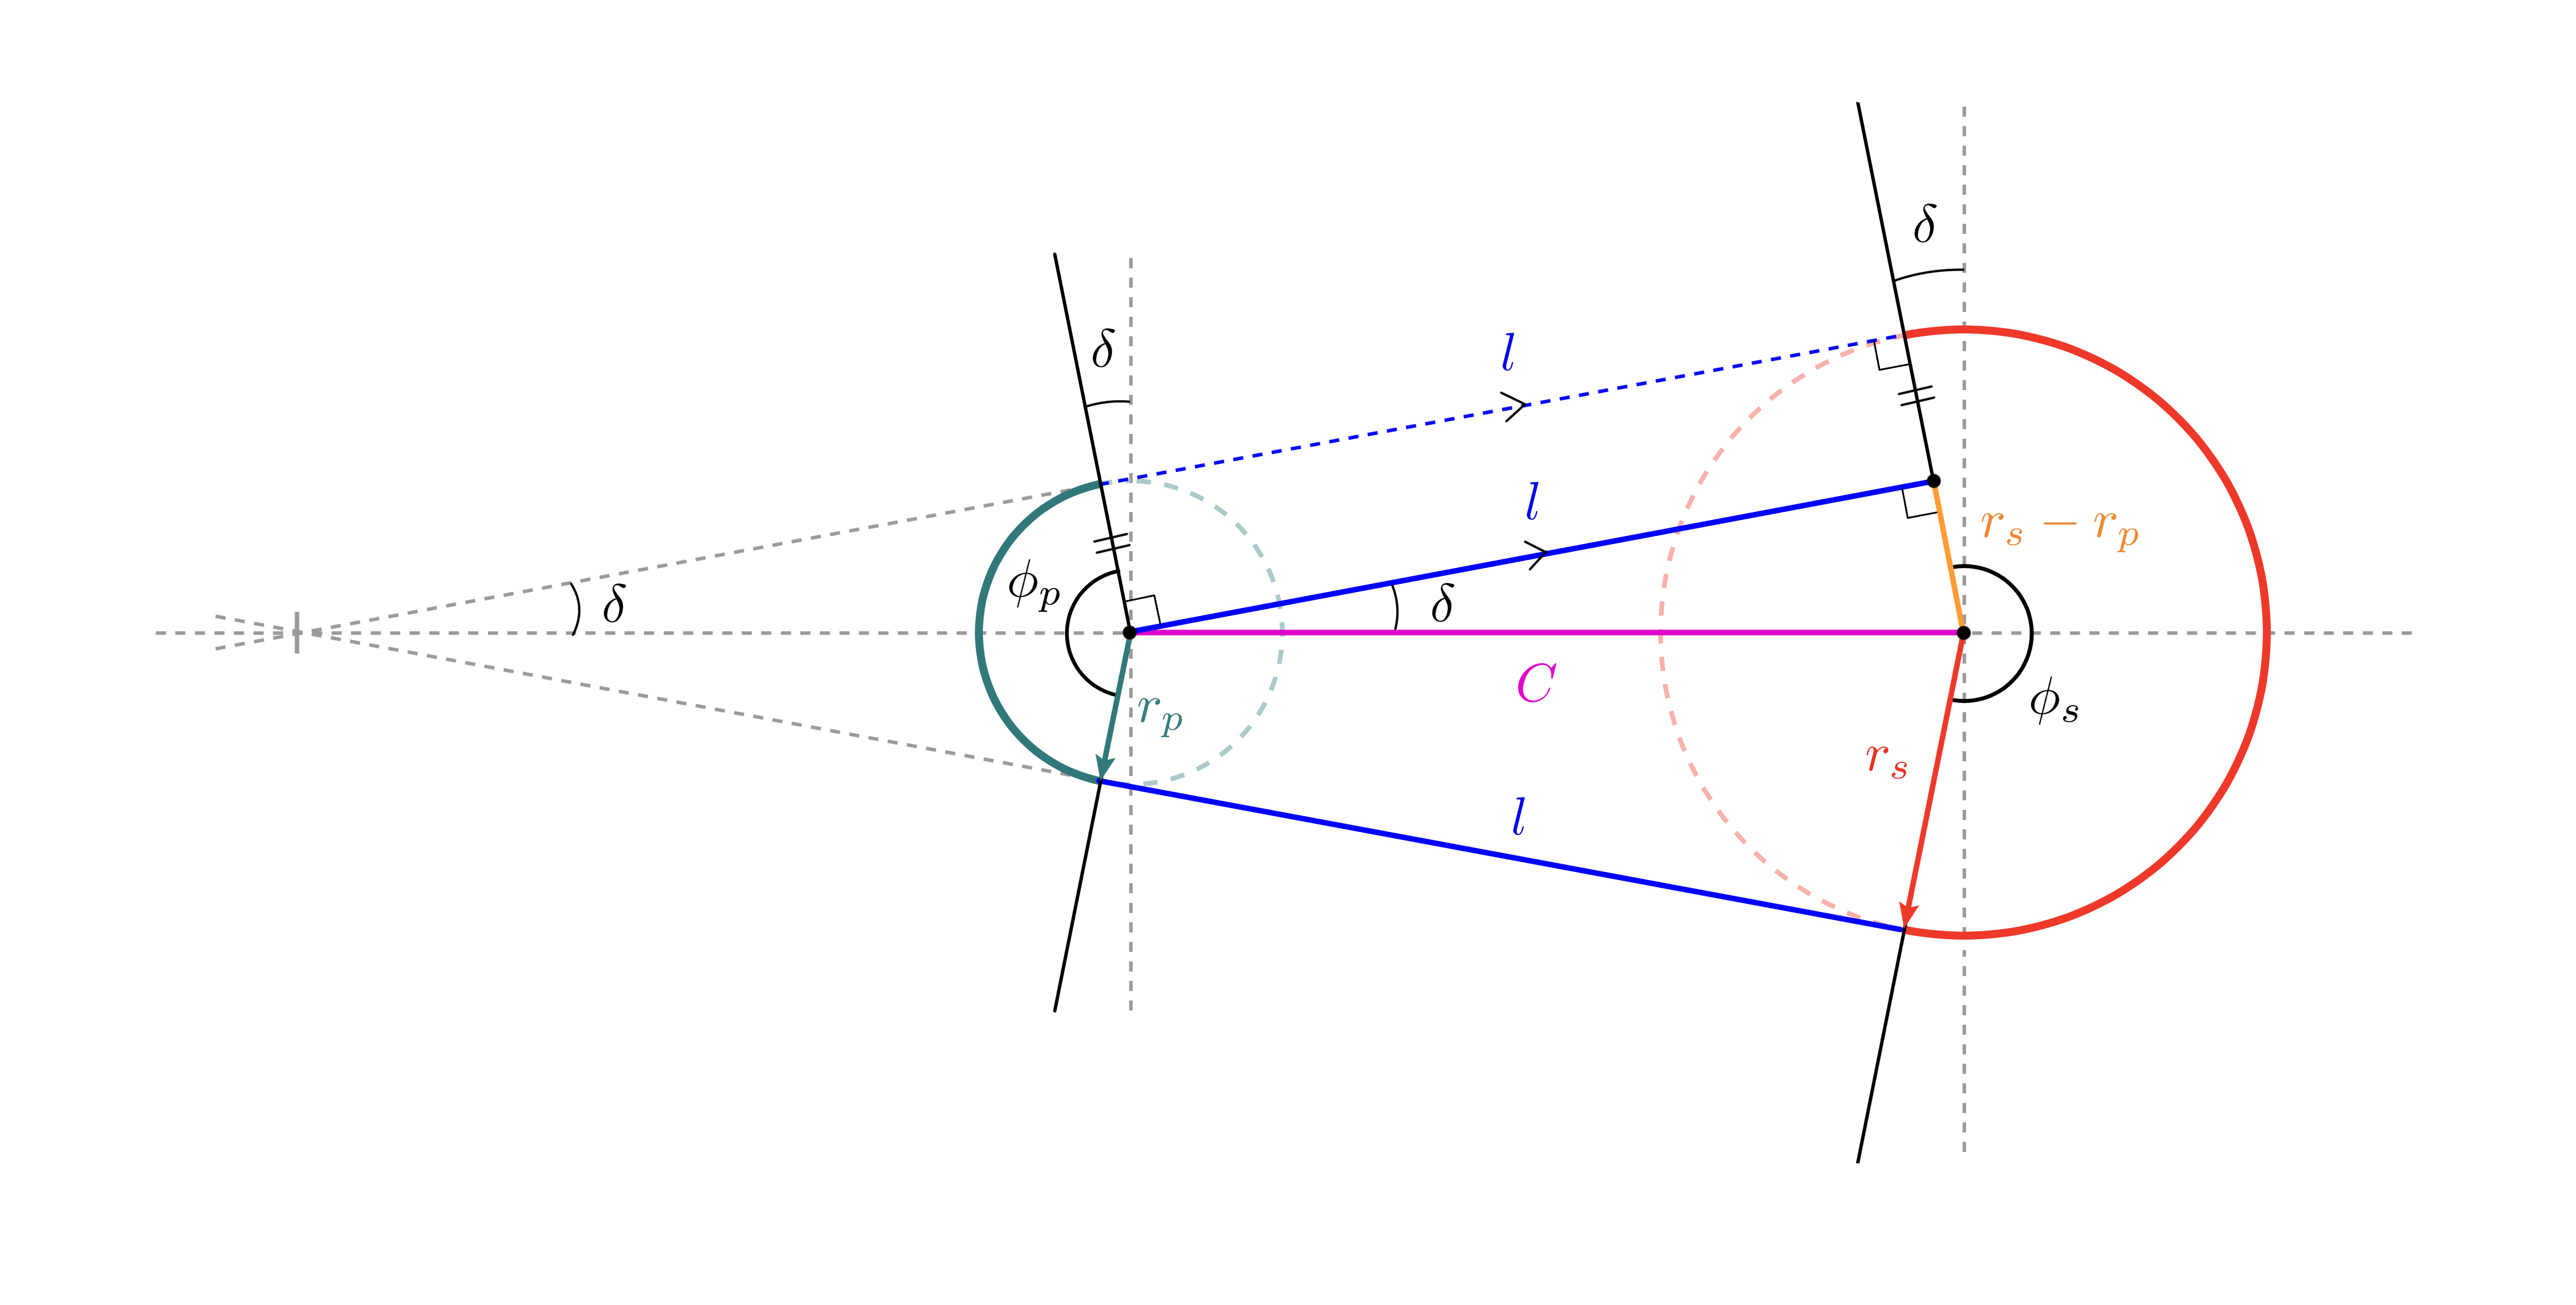
\includegraphics[width=\textwidth]
        {figures/geometry/belt_loop_geometry.png}
    \caption{
    Geometry of the complete belt loop. The belt path consists of two wrapped
    arcs and two equal straight spans of length \(l\). Unequal pulley radii
    incline the straight spans by the angle \(\delta\), producing the primary
    and secondary wrap angles \(\phi_p\) and \(\phi_s\).
    }
    \label{fig:belt_loop_geometry}
\end{figure}

Consider the right triangle in the upper span in
\Fig{fig:belt_loop_geometry}. The line joining the pulley centres forms its
hypotenuse and has length \(d_c\). One side lies along the straight belt span
and therefore has length \(l\).

The other side is perpendicular to the span. The primary and secondary radii
drawn to their respective contact points are also perpendicular to this span
and are therefore parallel. As shown by the orange construction in
\Fig{fig:belt_loop_geometry}, the difference between their lengths gives the
remaining side of the triangle, \(r_s-r_p\). The triangle therefore satisfies

\begin{equation}
    l^2+\left(r_s-r_p\right)^2=d_c^2,
\end{equation}

and the length of either straight span is

\begin{equation}
    l
    =
    \sqrt{d_c^2-\left(r_s-r_p\right)^2}.
    \label{eq:belt_straight_span_length}
\end{equation}

This expression requires

\begin{equation}
    \left|r_s-r_p\right|<d_c.
\end{equation}

This condition is already enforced by the physical separation of the
pulleys. The pulley circles must remain apart, requiring
\(d_c>r_s+r_p\), and \(r_s+r_p\) is necessarily greater than
\(\left|r_s-r_p\right|\).

The straight-span length accounts for only two parts of the belt path. The
two wrapped portions still depend on how the straight spans meet the pulleys.
If the pulley radii are equal, the spans are parallel to the line joining the
pulley centres and the belt wraps halfway around each pulley. Both wrap angles
are then equal to \(\pi\).

When the radii differ, the straight spans rotate through the angle
\(\delta\) shown in \Fig{fig:belt_loop_geometry}. The same right triangle gives

\begin{equation}
    \sin\delta
    =
    \frac{r_s-r_p}{d_c},
\end{equation}

and therefore

\begin{equation}
    \delta
    =
    \sin^{-1}\!\left(\frac{r_s-r_p}{d_c}\right).
    \label{eq:belt_span_angle}
\end{equation}

The angle \(\delta\) is signed. For the configuration shown,
\(r_s>r_p\), so \(\delta>0\). The primary wrap loses an angle
\(\delta\) at each end of its contact arc, while the secondary wrap gains the
same amount at each end. Their wrap angles are therefore

\begin{equation}
    \phi_p=\pi-2\delta,
    \qquad
    \phi_s=\pi+2\delta.
    \label{eq:pulley_wrap_angles}
\end{equation}

If \(r_p>r_s\), then \(\delta<0\), and the same equations automatically
reverse which pulley has the larger wrap angle.

The complete belt length follows by adding the two wrapped arcs and the two
straight spans. Substituting
\Cref{eq:belt_straight_span_length,eq:belt_span_angle,eq:pulley_wrap_angles}
into \Cref{eq:belt_length_components} gives

\bigeq{eq:belt_length_exact}
{Exact geometric belt length}
{
\begin{aligned}
L_{\mathrm{geo}}(r_p,r_s,d_c)
={}&
\pi\left(r_p+r_s\right)
\\
&+
2\left(r_s-r_p\right)
\sin^{-1}\!\left(\frac{r_s-r_p}{d_c}\right)
\\
&+
2\sqrt{d_c^2-\left(r_s-r_p\right)^2}
\end{aligned}
}

Each term still corresponds directly to part of the belt path. The first is
the combined half-circle contribution from the two pulley wraps. The second
accounts for the unequal wrap angles, and the third is the combined length of
the two straight spans.

For any chosen values of \(r_p\), \(r_s\), and \(d_c\),
\Cref{eq:belt_length_exact} tells us how much belt is required to follow that
path. The installed belt cannot change its total length as the pulleys shift.
Under \AssRef{assump:constant_belt_length}, every possible pulley position must
therefore satisfy

\begin{equation}
    L_{\mathrm{geo}}(r_p,r_s,d_c)=L_b,
    \label{eq:belt_length_compatibility}
\end{equation}

where \(L_b\) is the fixed length of the same outer-surface path described by
\(r_p\) and \(r_s\), consistent with the convention in
\Cref{eq:geometry_radius_convention}. This is the geometric compatibility
condition for the belt loop. Once any two of \(r_p\), \(r_s\), and \(d_c\) are
known, the condition determines the third.

For a particular CVT, the first quantity to determine is the centre distance
\(d_c\). The pulley radii change as the sheaves move, but the pulley shafts do
not move with them. Once the CVT is assembled, \(d_c\) remains fixed throughout
operation.

The fixed centre distance can be found from any installed pulley position
that can be measured. At that position, the belt length and the two pulley
radii are known. Denoting the measured radii by
\(r_{p,\mathrm{ref}}\) and \(r_{s,\mathrm{ref}}\), the only unknown in
\Cref{eq:belt_length_compatibility} is \(d_c\).

In the general unequal-radius case, \(d_c\) appears both inside the square root
and inside the inverse sine. The exact relation therefore cannot be
rearranged into a useful explicit expression for \(d_c\). Instead, the centre
distance is found with a one-dimensional root solve.

For a trial centre distance, the difference between the belt length required
by the geometry and the belt length actually available is

\begin{equation}
    \mathcal{R}_L(r_p,r_s,d_c)
    =
    L_{\mathrm{geo}}(r_p,r_s,d_c)-L_b.
    \label{eq:belt_length_residual}
\end{equation}

A positive residual means that the trial geometry requires more belt than is
available. A negative residual means that it requires less. The correct
centre distance is the value for which the required and available lengths
match:

\begin{equation}
    \mathcal{R}_L
    \left(
        r_{p,\mathrm{ref}},
        r_{s,\mathrm{ref}},
        d_c
    \right)
    =0.
    \label{eq:center_distance_root}
\end{equation}

The root solver varies \(d_c\) until this condition is satisfied.

Once the initial root solve has determined \(d_c\), both the centre distance and
the belt length are known constants. The compatibility condition can then be
used to connect the two pulley radii at every subsequent position.

Suppose the primary radius \(r_p\) is known. Substituting \(r_p\), \(d_c\), and
\(L_b\) into \Cref{eq:belt_length_residual} leaves the secondary radius as the
only unknown. Its compatible value is found from

\begin{equation}
    \mathcal{R}_L(r_p,r_s,d_c)=0
    \qquad
    \text{solved for } r_s.
    \label{eq:secondary_radius_compatibility}
\end{equation}

The resulting \(r_s\) is the secondary radius required for the same fixed
belt to pass around both pulleys. The calculation also works in the opposite
direction. If \(r_s\) is known instead, the compatible primary radius follows
from

\begin{equation}
    \mathcal{R}_L(r_p,r_s,d_c)=0
    \qquad
    \text{solved for } r_p.
    \label{eq:primary_radius_compatibility}
\end{equation}

Thus, once \(d_c\) has been established, either pulley radius can be used to
determine the other. The two radii remain local geometric quantities, but
they cannot vary independently while belonging to the same fixed-length belt
loop.

The arc-and-tangent construction used above is standard in belt-drive
geometry. \citet{BudynasNisbett2015} presents the same underlying construction
for relating pulley radii, straight spans, wrap angles, and total belt length.
The exact geometry is retained here because it provides the compatibility
relation between the two shifting pulleys.

The local relations \(r_p(x_p)\) and \(r_s(x_s)\) now describe how each
pulley produces its radius, while
\Cref{eq:belt_length_compatibility} describes which pairs of radii can belong
to the same belt loop. Combining these results gives the relationship between
the two local axial coordinates.
% --------------------------------------------------------------

% --------------------------------------------------------------
\subsection{From Local Pulley Coordinates to the Shift Coordinate}
\label{sec:pulley_coordinate_mapping}

The preceding geometry gives a local relation for each pulley: $x_p$
determines $r_p(x_p)$, and $x_s$ determines $r_s(x_s)$. A complete CVT
configuration, however, cannot be formed by choosing these positions
independently. Both radii must belong to the same belt loop of length $L_b$.
The remaining problem is therefore to identify the pairs $(x_p,x_s)$ that
satisfy this shared geometry.

For any proposed pair, the local pulley relations first give the two radii.
Substituting those radii into the belt-length residual gives

\begin{equation}
    \mathcal{R}_x(x_p,x_s)
    \equiv
    \mathcal{R}_L
    \!\left(
        r_p(x_p),
        r_s(x_s),
        d_c
    \right)
    =0.
    \label{eq:axial_coordinate_compatibility}
\end{equation}

Every pair that makes \Cref{eq:axial_coordinate_compatibility} equal to zero
is a possible position of the two pulleys. Together, these pairs form the
compatibility curve.

To reveal the shape of this curve, either local coordinate could be chosen as
a starting point. Take $x_p$ simply as an arbitrary choice. For each value of
$x_p$, the primary relation gives $r_p(x_p)$. The shaft spacing fixes $d_c$, and
$L_b$ remains fixed by \AssRef{assump:constant_belt_length}, so the belt-length
residual can then be solved for the required secondary radius $r_s$. The local
secondary relation finally gives the corresponding position $x_s$:

\[
    x_p
    \;\longrightarrow\;
    r_p(x_p)
    \;\longrightarrow\;
    r_s
    \;\longrightarrow\;
    x_s.
\]

Repeating these steps across the primary travel produces the representative
compatibility curve in \Fig{fig:pulley_coordinate_compatibility}.

\begin{figure}[H]
    \centering
    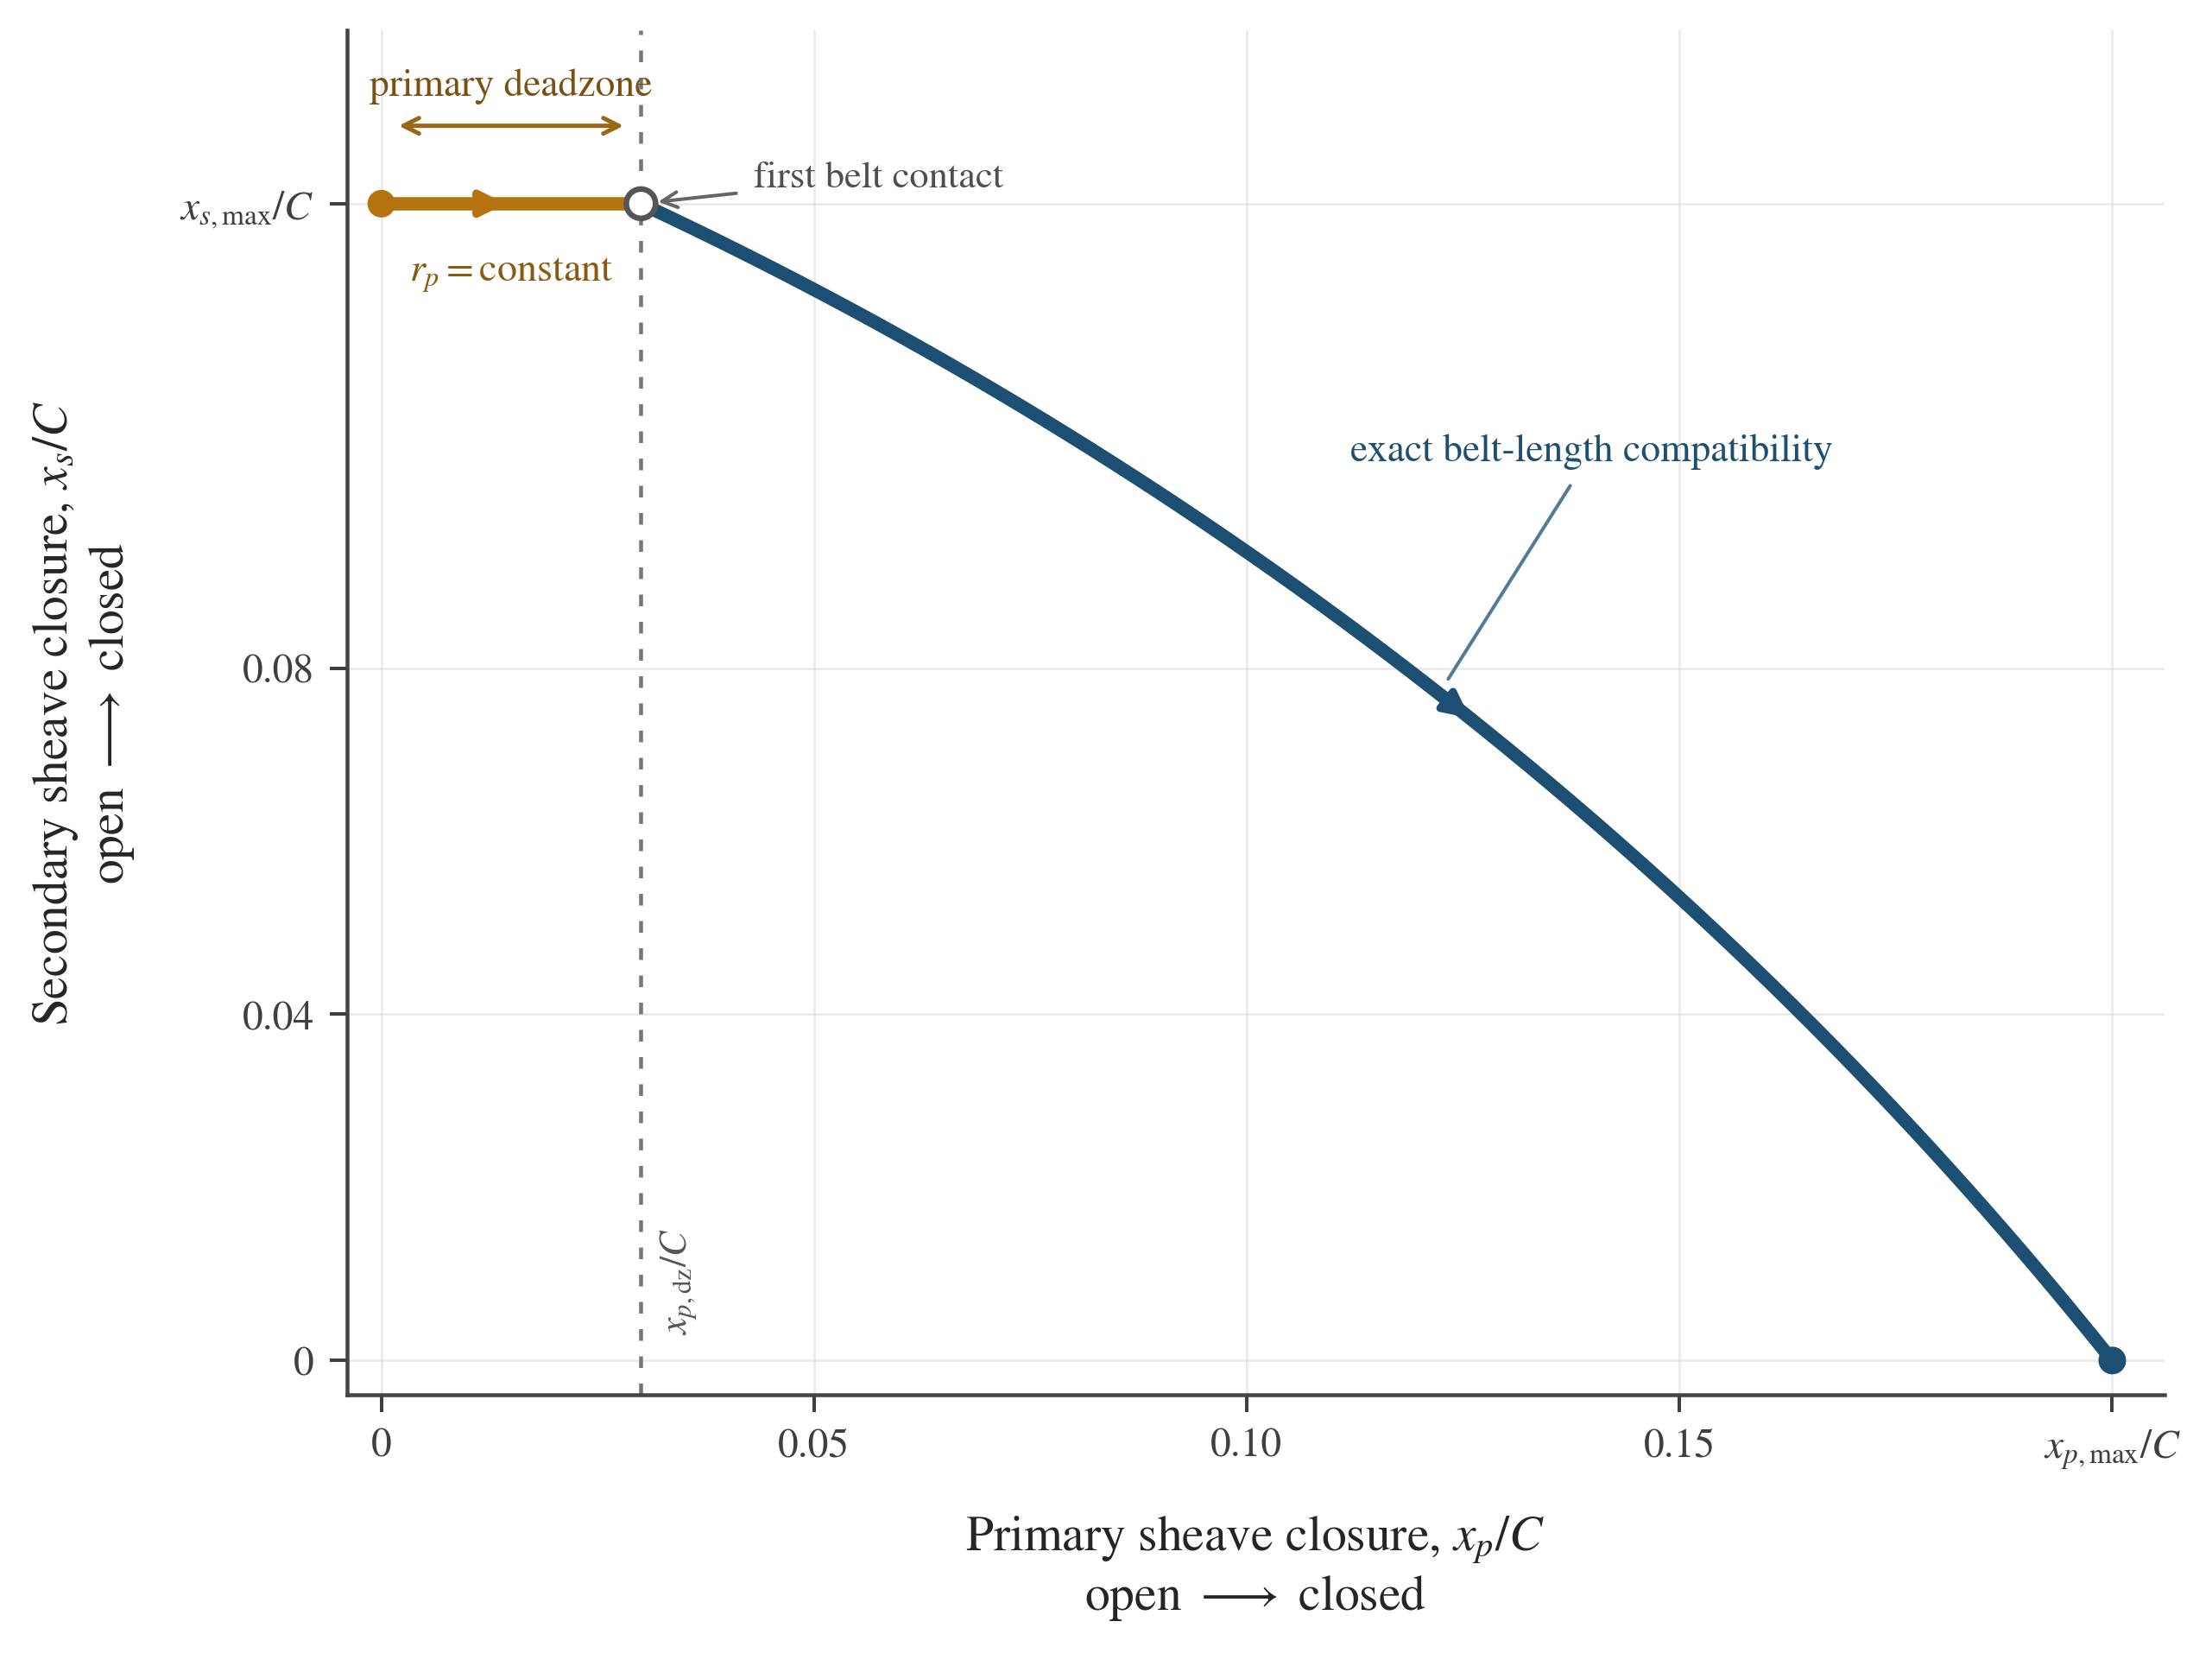
\includegraphics[width=0.94\textwidth]
        {figures/geometry/pulley_coordinate_compatibility.png}
    \caption{
    Representative compatibility curve between the local primary and
    secondary axial coordinates for an admissible belt--pulley geometry. Both
    coordinates are normalized by the same centre distance $d_c$, so their
    relative travel and the changing slope of the engaged branch are shown on
    a common scale. The dimensions are illustrative and do not represent a
    particular CVT.
    }
    \label{fig:pulley_coordinate_compatibility}
\end{figure}

The horizontal portion is created by the primary deadzone. While
$0\leq x_p<x_{p,\mathrm{dz}}$, the primary sheave closes only the clearance to
the belt. The primary radius remains fixed, so the compatible secondary radius
and position remain fixed as well.

Once the primary reaches the belt, further closure increases $r_p$. The fixed
belt loop then requires $r_s$ to decrease, which means that the secondary
opens and $x_s$ decreases. The two sheaves do not move by equal amounts, and
the resulting branch is not linear. Changing the radii alters both wrap
lengths and both straight spans, so the compatible secondary displacement
changes throughout the shift.

The curve also reveals which local coordinate can represent the complete
geometry. A vertical line at any $x_p$ meets the curve once, giving one
compatible $x_s$. At the deadzone height, however, a horizontal line meets
every $x_p$ between $0$ and $x_{p,\mathrm{dz}}$. Thus $x_s$ is a unique
function of $x_p$ over the full travel, whereas $x_p$ is not a unique function
of $x_s$.

The primary coordinate is therefore adopted as the system shift coordinate.
This is the same $s$ included in the state vector of
\Cref{sec:continuous_state_variables}:

\bigeq{eq:system_shift_coordinate}
{System shift coordinate}
{
    s\equiv x_p,
    \qquad
    x_p(s)=s,
    \qquad
    x_s=x_s(s)
}

The secondary mapping is then

\begin{equation}
    x_s(s)
    =
    \begin{cases}
        x_{s,\max},
        & 0\leq s<x_{p,\mathrm{dz}},\\[4pt]
        \displaystyle
        \operatorname*{root}_{0\leq x_s\leq x_{s,\max}}
        \!\left[\mathcal{R}_x(s,x_s)=0\right],
        & x_{p,\mathrm{dz}}\leq s\leq x_{p,\max}.
    \end{cases}
    \label{eq:secondary_coordinate_map}
\end{equation}

The first branch holds the secondary fixed while the primary closes its
clearance; the second returns the unique compatible position after belt
contact. Both give $x_{s,\max}$ at $s=x_{p,\mathrm{dz}}$, so the mapping is
continuous. The shift coordinate therefore determines both movable-sheave 
positions and, through the local pulley relations, both pulley radii. The 
position geometry is now complete. What remains is to determine how these 
positions and radii move when $s$ changes with time.

% --------------------------------------------------------------
\subsection{Pulley-Radius Rates}
\label{sec:pulley_radius_rates}

The shift coordinate now determines the positions of both movable sheaves and
the corresponding pulley radii. Its rate form asks the same geometric question
over a small motion: if the primary closes by an amount \(ds\), how far must
the secondary open, and how quickly do the two pulley radii change?

We first find how each local coordinate and pulley radius changes per unit
\(s\). Throughout this subsection, a prime denotes differentiation with
respect to \(s\). For either pulley \(j\in\{p,s\}\), the corresponding time
rates are then

\begin{equation}
    \dot x_j=x_j'(s)\dot s,
    \qquad
    \dot r_j=r_j'(s)\dot s.
    \label{eq:shift_to_time_rate}
\end{equation}

\paragraph{Primary radius rate}

The primary side follows immediately from the definition \(x_p(s)=s\):

\begin{equation}
    x_p'(s)=1,
    \qquad
    \dot x_p=\dot s.
    \label{eq:primary_axial_rate}
\end{equation}

The corresponding radius map is constant through the primary deadzone and
linear after the movable sheave reaches the belt. Differentiating
\Cref{eq:primary_local_radius_map} therefore gives

\begin{equation}
    r_p'(s)
    =
    \begin{cases}
        0,
        & 0\leq s<x_{p,\mathrm{dz}},\\[8pt]
        \displaystyle
        \frac{1}{2\tan\beta},
        & x_{p,\mathrm{dz}}<s\leq x_{p,\max}.
    \end{cases}
    \label{eq:primary_radius_shift_derivative}
\end{equation}

Multiplying this slope by \(\dot s\) gives

\bigeq{eq:primary_radius_rate}
{Primary Radius Rate}
{
\dot r_p
=
\begin{cases}
    0,
    & 0\leq s<x_{p,\mathrm{dz}},\\[10pt]
    \displaystyle
    \frac{\dot s}{2\tan\beta},
    & x_{p,\mathrm{dz}}<s\leq x_{p,\max}.
\end{cases}
}

Thus, the primary sheave can move while crossing the deadzone even though the
primary belt radius does not. After contact, the sheave angle fixes the radial
change produced by each unit of primary closure.

\paragraph{Secondary coordinate and radius rates}

The secondary requires one additional step. Its local pulley relation tells
us how \(r_s\) changes when \(x_s\) changes, but it does not tell us how far the
secondary must move. That motion is set by the fixed belt loop.

At every compatible position,

\begin{equation}
    L_{\mathrm{geo}}\!\left(r_p(s),r_s(s),d_c\right)=L_b.
    \label{eq:belt_length_along_shift}
\end{equation}

The centre distance \(d_c\) is fixed by the pulley shafts, while \(L_b\) is
constant under \AssRef{assump:constant_belt_length}. A small change in \(s\)
therefore cannot change the geometric length of the belt path:

\begin{equation}
    \frac{dL_{\mathrm{geo}}}{ds}=0.
    \label{eq:belt_length_shift_derivative_zero}
\end{equation}

Both radii change during this motion. The change caused by \(r_p\) is the
sensitivity of the belt length to \(r_p\), multiplied by the actual rate
\(r_p'\). The secondary contributes in the same way. Applying the chain rule
to \Cref{eq:belt_length_along_shift} gives

\begin{equation}
    \frac{\partial L_{\mathrm{geo}}}{\partial r_p}r_p'
    +
    \frac{\partial L_{\mathrm{geo}}}{\partial r_s}r_s'
    =0.
    \label{eq:radius_slope_compatibility}
\end{equation}

The two partial derivatives have a direct purpose: each tells us how much
additional belt path would be required if one pulley radius increased while
the other radius remained fixed. The actual pulley motion must make these two
changes cancel. We therefore calculate the two sensitivities next.

The span angle and straight-span length entering the belt-length relation were
derived in
\Cref{eq:belt_span_angle,eq:belt_straight_span_length}. Writing them together
in the form needed for differentiation,

\begin{equation}
    \delta
    =
    \sin^{-1}\!\left(\frac{r_s-r_p}{d_c}\right),
    \qquad
    l
    =
    \sqrt{d_c^2-(r_s-r_p)^2},
    \label{eq:belt_rate_geometry_recalled}
\end{equation}

Here, \(\delta\) sets the wrap angles through
\Cref{eq:pulley_wrap_angles}, while \(l\) is the length of either straight
span. Using these quantities, the exact path length from
\Cref{eq:belt_length_exact} is

\begin{equation}
    L_{\mathrm{geo}}
    =
    \pi(r_p+r_s)
    +
    2(r_s-r_p)\delta
    +
    2l.
    \label{eq:belt_length_rate_form}
\end{equation}

First, hold \(r_s\) and \(d_c\) fixed and increase \(r_p\). The radius difference
\(r_s-r_p\) then decreases at the same rate:

\begin{equation}
    \frac{\partial(r_s-r_p)}{\partial r_p}=-1.
    \label{eq:radius_difference_primary_derivative}
\end{equation}

Using this result in the definitions of \(\delta\) and \(l\) gives

\begin{align}
    \frac{\partial\delta}{\partial r_p}
    &=
    \frac{1}
    {\sqrt{1-\left(\dfrac{r_s-r_p}{d_c}\right)^2}}
    \left(-\frac{1}{d_c}\right)
    \nonumber\\
    &=
    -\frac{1}
    {\sqrt{d_c^2-(r_s-r_p)^2}}
    =
    -\frac{1}{l},
    \label{eq:span_angle_primary_derivative}\\[8pt]
    \frac{\partial l}{\partial r_p}
    &=
    \frac{1}
    {2\sqrt{d_c^2-(r_s-r_p)^2}}
    \left[2(r_s-r_p)\right]
    \nonumber\\
    &=
    \frac{r_s-r_p}{l}.
    \label{eq:straight_span_primary_derivative}
\end{align}

We can now differentiate the complete path length in
\Cref{eq:belt_length_rate_form}. The first term differentiates directly, the
wrap correction requires the product rule, and the final term contains the
changing straight spans:

\begin{align}
    \frac{\partial L_{\mathrm{geo}}}{\partial r_p}
    &=
    \pi
    +
    2\left[
        (-1)\delta
        +
        (r_s-r_p)\left(-\frac{1}{l}\right)
    \right]
    +
    2\left(\frac{r_s-r_p}{l}\right)
    \nonumber\\
    &=
    \pi-2\delta
    \nonumber\\
    &=
    \phi_p.
    \label{eq:belt_length_primary_sensitivity}
\end{align}

The two terms containing \((r_s-r_p)/l\) cancel. The remaining sensitivity is
the primary wrap angle.

The secondary calculation follows the same path, but increasing \(r_s\)
increases the radius difference:

\begin{equation}
    \frac{\partial(r_s-r_p)}{\partial r_s}=1.
    \label{eq:radius_difference_secondary_derivative}
\end{equation}

The corresponding derivatives of \(\delta\) and \(l\) are

\begin{align}
    \frac{\partial\delta}{\partial r_s}
    &=
    \frac{1}
    {\sqrt{1-\left(\dfrac{r_s-r_p}{d_c}\right)^2}}
    \left(\frac{1}{d_c}\right)
    \nonumber\\
    &=
    \frac{1}{l},
    \label{eq:span_angle_secondary_derivative}\\[8pt]
    \frac{\partial l}{\partial r_s}
    &=
    \frac{1}
    {2\sqrt{d_c^2-(r_s-r_p)^2}}
    \left[-2(r_s-r_p)\right]
    \nonumber\\
    &=
    -\frac{r_s-r_p}{l}.
    \label{eq:straight_span_secondary_derivative}
\end{align}

Differentiating the full path length with these signs gives

\begin{align}
    \frac{\partial L_{\mathrm{geo}}}{\partial r_s}
    &=
    \pi
    +
    2\left[
        (1)\delta
        +
        (r_s-r_p)\left(\frac{1}{l}\right)
    \right]
    +
    2\left(-\frac{r_s-r_p}{l}\right)
    \nonumber\\
    &=
    \pi+2\delta
    \nonumber\\
    &=
    \phi_s.
    \label{eq:belt_length_secondary_sensitivity}
\end{align}

Again, the terms involving the changing straight-span length cancel. The
sensitivity to the secondary radius is the secondary wrap angle. Together,

\begin{equation}
    \frac{\partial L_{\mathrm{geo}}}{\partial r_p}
    =
    \phi_p,
    \qquad
    \frac{\partial L_{\mathrm{geo}}}{\partial r_s}
    =
    \phi_s.
    \label{eq:belt_length_radius_sensitivities}
\end{equation}

This result also has a simple geometric interpretation. If one pulley radius
increases by a small amount while the other is held fixed, the required belt
path increases by that radial change multiplied by the angle over which the
belt wraps the pulley. The remaining changes in the tangent geometry cancel
one another.

Returning to the fixed-length condition
\Cref{eq:radius_slope_compatibility}, the two radial changes must therefore
satisfy

\begin{equation}
    \phi_p r_p'
    +
    \phi_s r_s'
    =0.
    \label{eq:wrap_weighted_radius_slope_balance}
\end{equation}

After primary contact, the local pulley relation gives the same
axial-to-radial slope on both pulleys. Since \(x_p'=1\),

\begin{equation}
    r_p'
    =
    \frac{1}{2\tan\beta},
    \qquad
    r_s'
    =
    \frac{1}{2\tan\beta}x_s'.
    \label{eq:engaged_local_radius_slopes}
\end{equation}

Substituting these two slopes into
\Cref{eq:wrap_weighted_radius_slope_balance} gives

\begin{equation}
    \phi_p
    \left(\frac{1}{2\tan\beta}\right)
    +
    \phi_s
    \left(\frac{1}{2\tan\beta}x_s'\right)
    =0.
    \label{eq:secondary_coordinate_slope_substitution}
\end{equation}

The common local pulley slope cancels, leaving

\begin{equation}
    \phi_p+\phi_s x_s'=0.
    \label{eq:secondary_coordinate_slope_balance}
\end{equation}

Solving for the slope of the secondary mapping gives

\bigeq{eq:secondary_coordinate_slope}
{Secondary Coordinate Slope}
{
x_s'(s)
=
\begin{cases}
    0,
    & 0\leq s<x_{p,\mathrm{dz}},\\[10pt]
    \displaystyle
    -\frac{\phi_p}{\phi_s},
    & x_{p,\mathrm{dz}}<s\leq x_{p,\max}.
\end{cases}
}

Within the deadzone, the primary radius does not change, so neither the
compatible secondary radius nor \(x_s\) changes. After contact,
\(x_s'<0\): primary closure requires the secondary to open. Its magnitude is
not generally one and changes with the two wrap angles, which is why the
engaged branch in \Fig{fig:pulley_coordinate_compatibility} is curved rather
than straight.

The time rate of the secondary coordinate is now obtained by multiplying this
slope by \(\dot s\):

\begin{equation}
    \dot x_s
    =
    x_s'(s)\dot s
    =
    \begin{cases}
        0,
        & 0\leq s<x_{p,\mathrm{dz}},\\[10pt]
        \displaystyle
        -\frac{\phi_p}{\phi_s}\dot s,
        & x_{p,\mathrm{dz}}<s\leq x_{p,\max}.
    \end{cases}
    \label{eq:secondary_axial_rate}
\end{equation}

Applying the local axial-to-radial slope once more gives the secondary radius
rate:

\bigeq{eq:secondary_radius_rate}
{Secondary Radius Rate}
{
\dot r_s
=
\begin{cases}
    0,
    & 0\leq s<x_{p,\mathrm{dz}},\\[12pt]
    \displaystyle
    -\frac{\phi_p}{\phi_s}
    \frac{\dot s}{2\tan\beta},
    & x_{p,\mathrm{dz}}<s\leq x_{p,\max}.
\end{cases}
}

The rates above were written for \(r_p\) and \(r_s\), which denote the
outer-surface radii. The inner surface, cord line, and mass centre remain at
fixed depths within the belt cross-section. When the belt moves radially on
either pulley, all four reference radii therefore change by exactly the same
amount. For either pulley \(j\in\{p,s\}\),

\begin{equation}
    r'_j
    =
    r'_{j,\mathrm{inner}}
    =
    r'_{j,\mathrm{eff}}
    =
    r'_{j,\mathrm{cm}},
    \qquad
    \dot r_j
    =
    \dot r_{j,\mathrm{inner}}
    =
    \dot r_{j,\mathrm{eff}}
    =
    \dot r_{j,\mathrm{cm}}.
    \label{eq:radial_reference_rate_equivalence}
\end{equation}

The choice of reference changes the absolute radius, but not its rate. The two
pulley-radius rates are now determined by \(s\) and \(\dot s\). However, the
secondary multiplier
\(-\phi_p/\phi_s\) changes as the radii and wrap angles change. Even if
\(\dot s\) is constant, the secondary rate is not. Its acceleration must
therefore include the changing slope of the compatibility curve.


% --------------------------------------------------------------
\subsection{Pulley-Radius Accelerations}
\label{sec:pulley_radius_accelerations}

The pulley-radius rates in
\Cref{eq:primary_radius_rate,eq:secondary_radius_rate} were obtained by
multiplying the slope of each geometric mapping by the shift velocity
\(\dot s\). Their accelerations follow by asking how those rates change. On
the primary, the mapping slope is constant within each branch. On the
secondary, the slope in \Cref{eq:secondary_coordinate_slope} changes as the
pulley radii and wrap angles change. The secondary acceleration must therefore
account for both the imposed shift acceleration and the changing geometric
slope.

\paragraph{Primary radius acceleration}

The primary coordinate requires no additional geometry. The system-coordinate
definition in \Cref{eq:system_shift_coordinate} gives \(x_p(s)=s\), so

\begin{equation}
    x_p'(s)=1,
    \qquad
    x_p''(s)=0,
    \label{eq:primary_coordinate_derivatives}
\end{equation}

and therefore

\begin{equation}
    \dot x_p=\dot s,
    \qquad
    \ddot x_p=\ddot s.
    \label{eq:primary_axial_acceleration}
\end{equation}

The general shift-to-time relation in \Cref{eq:shift_to_time_rate} gives the
primary radius rate in the form

\begin{equation}
    \dot r_p=r_p'(s)\dot s.
    \label{eq:primary_radius_rate_acceleration_start}
\end{equation}

Differentiating this product with respect to time gives

\begin{align}
    \ddot r_p
    &=
    \frac{d}{dt}
    \left[
        r_p'(s)\dot s
    \right]
    \nonumber\\
    &=
    \frac{d r_p'}{dt}\dot s
    +
    r_p'(s)\ddot s.
    \label{eq:primary_radius_acceleration_product_rule}
\end{align}

Because \(r_p'\) is itself a function of \(s\),

\begin{equation}
    \frac{d r_p'}{dt}
    =
    r_p''(s)\dot s.
    \label{eq:primary_radius_slope_time_derivative}
\end{equation}

Substituting \Cref{eq:primary_radius_slope_time_derivative} into
\Cref{eq:primary_radius_acceleration_product_rule} gives

\begin{equation}
    \ddot r_p
    =
    r_p''(s)\dot s^2
    +
    r_p'(s)\ddot s.
    \label{eq:primary_radius_acceleration_chain}
\end{equation}

Within either smooth branch of the primary radius map,
\(r_p'(s)\) is constant. Hence

\begin{equation}
    r_p''(s)=0.
    \label{eq:primary_radius_mapping_curvature}
\end{equation}

Using the primary slopes from
\Cref{eq:primary_radius_shift_derivative}, the primary radius acceleration is

\bigeq{eq:primary_radius_acceleration}
{Primary Radius Acceleration}
{
\ddot r_p
=
\begin{cases}
    0,
    & 0\leq s<x_{p,\mathrm{dz}},\\[10pt]
    \displaystyle
    \frac{\ddot s}{2\tan\beta},
    & x_{p,\mathrm{dz}}<s\leq x_{p,\max}.
\end{cases}
}

The result is direct: within the deadzone the primary radius remains fixed,
while after contact the shift acceleration is converted into radial
acceleration by the same constant sheave slope found in
\Cref{eq:primary_radius_shift_derivative}.

\paragraph{Secondary coordinate curvature}

The secondary mapping is not linear after contact. Its first derivative was
found from the fixed-length rate balance in
\Cref{eq:secondary_coordinate_slope_balance}:

\[
    \phi_p+\phi_s x_s'=0.
\]

The balance in \Cref{eq:secondary_coordinate_slope_balance} contains the
information needed for the second derivative. We will differentiate it once
more with respect to \(s\), which first requires the rates at which the two
wrap angles change with \(s\).

The required geometric quantities were defined in
\Cref{eq:belt_span_angle,eq:pulley_wrap_angles}. Written together, they are

\begin{equation}
    \delta
    =
    \sin^{-1}\!\left(\frac{r_s-r_p}{d_c}\right),
    \qquad
    \phi_p=\pi-2\delta,
    \qquad
    \phi_s=\pi+2\delta.
    \label{eq:wrap_geometry_for_acceleration}
\end{equation}

As \(s\) changes, both \(r_p\) and \(r_s\) change, so the radius difference
inside \(\delta\) changes at the rate

\begin{equation}
    \frac{d}{ds}(r_s-r_p)
    =
    r_s'-r_p'.
    \label{eq:radius_difference_shift_derivative}
\end{equation}

Applying the chain rule to \(\delta\), and using the straight-span length from
\Cref{eq:belt_straight_span_length} in the final line, gives

\begin{align}
    \delta'
    &=
    \frac{1}
    {\sqrt{1-\left(\dfrac{r_s-r_p}{d_c}\right)^2}}
    \left(
        \frac{r_s'-r_p'}{d_c}
    \right)
    \nonumber\\
    &=
    \frac{r_s'-r_p'}
    {\sqrt{d_c^2-(r_s-r_p)^2}}
    \nonumber\\
    &=
    \frac{r_s'-r_p'}{l}.
    \label{eq:span_angle_shift_derivative}
\end{align}

After primary contact, the local pulley slopes are given by
\Cref{eq:engaged_local_radius_slopes}:

\[
    r_p'
    =
    \frac{1}{2\tan\beta},
    \qquad
    r_s'
    =
    \frac{x_s'}{2\tan\beta}.
\]

Substituting these slopes into
\Cref{eq:span_angle_shift_derivative} gives

\begin{align}
    \delta'
    &=
    \frac{
        \dfrac{x_s'}{2\tan\beta}
        -
        \dfrac{1}{2\tan\beta}
    }{l}
    \nonumber\\
    &=
    \frac{x_s'-1}{2l\tan\beta}.
    \label{eq:span_angle_shift_derivative_coordinate_form}
\end{align}

The wrap-angle derivatives now follow directly from
\Cref{eq:wrap_geometry_for_acceleration}:

\begin{equation}
    \phi_p'=-2\delta',
    \qquad
    \phi_s'=2\delta'.
    \label{eq:wrap_angle_shift_derivatives}
\end{equation}

We can now differentiate the secondary slope balance in
\Cref{eq:secondary_coordinate_slope_balance}. The primary term
contributes \(\phi_p'\), while the secondary term requires the product rule
because both \(\phi_s\) and \(x_s'\) change with \(s\):

\begin{align}
    0
    &=
    \frac{d}{ds}
    \left(
        \phi_p+\phi_s x_s'
    \right)
    \nonumber\\
    &=
    \phi_p'
    +
    \phi_s'x_s'
    +
    \phi_s x_s''.
    \label{eq:secondary_coordinate_curvature_balance}
\end{align}

Substituting the wrap-angle derivatives from
\Cref{eq:wrap_angle_shift_derivatives} gives

\begin{equation}
    -2\delta'
    +
    2\delta'x_s'
    +
    \phi_s x_s''
    =0.
    \label{eq:secondary_coordinate_curvature_delta_form}
\end{equation}

Solving first for \(x_s''\),

\begin{align}
    \phi_s x_s''
    &=
    2\delta'(1-x_s'),
    \nonumber\\
    x_s''
    &=
    \frac{2\delta'(1-x_s')}{\phi_s}.
    \label{eq:secondary_coordinate_curvature_first_form}
\end{align}

Using the expression for \(\delta'\) from
\Cref{eq:span_angle_shift_derivative_coordinate_form},

\begin{align}
    x_s''
    &=
    \frac{2}{\phi_s}
    \left(
        \frac{x_s'-1}{2l\tan\beta}
    \right)
    (1-x_s')
    \nonumber\\
    &=
    -\frac{(1-x_s')^2}
    {\phi_s l\tan\beta}.
    \label{eq:secondary_coordinate_curvature_slope_form}
\end{align}

On the engaged branch, the first-derivative result in
\Cref{eq:secondary_coordinate_slope} gives
\(x_s'=-\phi_p/\phi_s\). The remaining factor can therefore be simplified:

\begin{align}
    1-x_s'
    &=
    1+\frac{\phi_p}{\phi_s}
    \nonumber\\
    &=
    \frac{\phi_s+\phi_p}{\phi_s}
    \nonumber\\
    &=
    \frac{2\pi}{\phi_s},
    \label{eq:secondary_coordinate_one_minus_slope}
\end{align}

where \(\phi_p+\phi_s=2\pi\) follows from
\Cref{eq:pulley_wrap_angles}. Substituting this result into
\Cref{eq:secondary_coordinate_curvature_slope_form} gives the curvature of
the secondary coordinate mapping:

\bigeq{eq:secondary_coordinate_curvature}
{Secondary Coordinate Curvature}
{
x_s''(s)
=
\begin{cases}
    0,
    & 0\leq s<x_{p,\mathrm{dz}},\\[12pt]
    \displaystyle
    -\frac{4\pi^2}
    {\phi_s^3 l\tan\beta},
    & x_{p,\mathrm{dz}}<s\leq x_{p,\max}.
\end{cases}
}

The deadzone branch in \Cref{eq:secondary_coordinate_map} is horizontal, so
both \(x_s'\) and \(x_s''\) are zero there. On the engaged branch,
\(x_s''<0\): as the primary closes, the secondary mapping becomes
progressively steeper in the opening direction.

\paragraph{Secondary axial and radial accelerations}

The curvature in \Cref{eq:secondary_coordinate_curvature} describes how the
slope of the compatibility curve changes with position. To convert it into
acceleration, begin with the secondary axial velocity from
\Cref{eq:secondary_axial_rate}:

\[
    \dot x_s=x_s'(s)\dot s.
\]

Differentiating with respect to time gives

\begin{align}
    \ddot x_s
    &=
    \frac{d}{dt}
    \left[
        x_s'(s)\dot s
    \right]
    \nonumber\\
    &=
    \frac{d x_s'}{dt}\dot s
    +
    x_s'(s)\ddot s.
    \label{eq:secondary_axial_acceleration_product_rule}
\end{align}

Because \(x_s'\) changes only through \(s\),

\begin{equation}
    \frac{d x_s'}{dt}
    =
    x_s''(s)\dot s.
    \label{eq:secondary_slope_time_derivative}
\end{equation}

The secondary axial acceleration is therefore

\begin{equation}
    \ddot x_s
    =
    x_s'(s)\ddot s
    +
    x_s''(s)\dot s^2.
    \label{eq:secondary_axial_acceleration_chain}
\end{equation}

Substituting the slope from \Cref{eq:secondary_coordinate_slope} and the
curvature from \Cref{eq:secondary_coordinate_curvature} gives

\bigeq{eq:secondary_axial_acceleration}
{Secondary Axial Acceleration}
{
\ddot x_s
=
\begin{cases}
    0,
    & 0\leq s<x_{p,\mathrm{dz}},\\[12pt]
    \displaystyle
    -\frac{\phi_p}{\phi_s}\ddot s
    -
    \frac{4\pi^2}
    {\phi_s^3 l\tan\beta}\dot s^2,
    & x_{p,\mathrm{dz}}<s\leq x_{p,\max}.
\end{cases}
}

The local radius derivative in \Cref{eq:local_radius_position_derivative} is
the constant \(1/(2\tan\beta)\). Applying it to the secondary gives

\begin{equation}
    \ddot r_s
    =
    \frac{1}{2\tan\beta}\ddot x_s.
    \label{eq:secondary_local_acceleration_map}
\end{equation}

Substituting \Cref{eq:secondary_axial_acceleration} into
\Cref{eq:secondary_local_acceleration_map} gives

\bigeq{eq:secondary_radius_acceleration}
{Secondary Radius Acceleration}
{
\ddot r_s
=
\begin{cases}
    0,
    & 0\leq s<x_{p,\mathrm{dz}},\\[14pt]
    \displaystyle
    -\frac{\phi_p}{\phi_s}
    \frac{\ddot s}{2\tan\beta}
    -
    \frac{2\pi^2}
    {\phi_s^3 l\tan^2\beta}\dot s^2,
    & x_{p,\mathrm{dz}}<s\leq x_{p,\max}.
\end{cases}
}

The two terms have different physical origins. The first comes from the
imposed shift acceleration, converted through the coordinate slope in
\Cref{eq:secondary_coordinate_slope} and the local pulley slope in
\Cref{eq:local_radius_position_derivative}. The second comes from the
curvature in \Cref{eq:secondary_coordinate_curvature}: even when
\(\ddot s=0\), moving through the engaged branch changes
\(-\phi_p/\phi_s\), so the secondary velocity continues to change.

As with the radius rates, the fixed offsets between the four radial references
give, for either pulley \(j\in\{p,s\}\),

\begin{equation}
    \ddot r_j
    =
    \ddot r_{j,\mathrm{inner}}
    =
    \ddot r_{j,\mathrm{eff}}
    =
    \ddot r_{j,\mathrm{cm}}.
    \label{eq:local_radius_acceleration_equivalence}
\end{equation}

\begin{remarkbox}[Remark (Deadzone Boundary)]
The idealized maps in
\Cref{eq:primary_local_radius_map,eq:secondary_coordinate_map} change slope
when the primary first reaches the belt at \(s=x_{p,\mathrm{dz}}\). Their
first derivatives therefore change discontinuously, and their ordinary second
derivatives are not defined at that single point. The acceleration relations
in \Cref{eq:primary_radius_acceleration,eq:secondary_radius_acceleration}
apply within the deadzone and engaged branches, while first contact is treated
as the transition between them.

\end{remarkbox}

% --------------------------------------------------------------
\subsection{Geometric Closure and Model Scope}
\label{sec:geometry_conclusion}

Specifying the shift state now determines the complete modeled pulley
geometry. The definition in \Cref{eq:system_shift_coordinate} sets the primary
position directly, while \Cref{eq:secondary_coordinate_map} gives the unique
compatible secondary position. The local pulley maps in
\Cref{eq:local_radius_map,eq:primary_local_radius_map} convert those two
positions into the outer-surface radii used to describe the belt path.
Finally, the rate and acceleration relations in
\Cref{eq:primary_radius_rate,eq:secondary_radius_rate,%
eq:primary_radius_acceleration,eq:secondary_radius_acceleration} determine how
those radii move. Thus, for any admissible shift state,

\[
    \left(s,\dot s,\ddot s\right)
    \quad\longmapsto\quad
    \left(
        r_p,\dot r_p,\ddot r_p,
        r_s,\dot r_s,\ddot r_s
    \right).
\]

Here \(r_p\) and \(r_s\) retain the outer-surface convention used throughout
the geometric development. The corresponding inner-surface, effective, and
centre-of-mass radii follow directly from their fixed positions within the
belt cross-section. Nothing else has to be solved for.

These results follow from the geometry derived above under the idealizations
stated in \Sec{sec:assumptions}. The belt cross-section and total length remain
fixed under \AssRef{assump:fixed-belt-cross-section} and
\AssRef{assump:constant_belt_length}, while
\AssRef{assump:prescribed_belt_path} constrains the belt to circular wraps and
straight tangent spans. Together with the aligned pulley axes and fixed centre
distance of \AssRef{assump:axis_alignment}, these conditions leave one modeled
belt path for each admissible value of \(s\).

\paragraph{Relation to prior transient models}

These choices also define the level of detail represented by the present
geometry. It determines the complete belt path that is globally compatible
with the imposed shift position, but it does not track the trajectory of each
belt element through the pulley wraps.

\citet{DuanEtAl2016} begin from closely related open-belt arc-and-tangent
geometry and the same wedge relationship between movable-sheave motion and
nominal radius motion. Their chain-CVT formulation retains additional internal
deformation. Chain extension and its rate contribute to the span tension, and
pulley deformation allows the local radius followed by a chain element to
differ from the nominal pulley radius. The present formulation instead fixes
the belt length through \AssRef{assump:constant_belt_length} and prescribes the
arc-and-tangent belt path through \AssRef{assump:prescribed_belt_path}. Consequently, elastic
path-length change and deformation-driven departure from that prescribed path
are not represented in this geometric closure.

Rubber-belt transient models resolve the same shifting process at several
levels of detail. Analytical shift-mechanics models, such as those of
\citet{Sorge2008} and \citet{CammalleriSorge2009}, describe local radial belt
migration through a pulley wrap and couple it to circumferential transport,
sliding, and the mechanics of the contact region. Discretized rubber-belt
models, such as those of \citet{JulioPlante2011} and \citet{Ballew2015},
instead obtain the evolving belt geometry from the motion and contact state of
individual belt elements. These approaches can resolve local deformation,
tension redistribution, and contact migration in greater detail, but require
additional spatial or nodal states and the contact laws that govern them.

The distinction is therefore one of model resolution. The present formulation
uses the global compatibility condition in \Cref{eq:belt_length_compatibility}
to find the representative pulley-radius pair and its derivatives directly
from \(s\), \(\dot s\), and \(\ddot s\). The cited transient models additionally
ask how the belt or chain deforms and migrates within that path. Those internal
motions lie outside the present geometric layer; within the assumptions stated
above, the global pulley geometry and its motion are fully determined.

This closure determines which sheave and radius motions are compatible with
the modeled belt path, but it does not determine which compatible acceleration
occurs. In particular, every acceleration relation above still contains the
shift acceleration \(\ddot s\). Its value must be consistent with the forces
and inertias acting on the two movable pulley assemblies.
% --------------------------------------------------------------


% --------------------------------------------------------------

\section{Axial Actuation and Sheave Balances}
\label{sec:axial_actuation_balances}

The preceding section established how the two movable sheaves must move
together. It did not determine the motion itself. That requires the forces
acting on each movable assembly and the inertia that those forces must
accelerate.

The primary and secondary remain separate mechanisms even though the belt
geometry couples their positions. Each has its own actuator, spring, moving
hardware, and belt reaction, so each must satisfy its own axial equation of
motion. We therefore complete the primary balance in its local coordinate
\(x_p\), then do the same for the secondary in \(x_s\). Once each mechanism has
been interpreted and every local force has been derived, the geometric maps
developed above in \Cref{sec:geometry} express both balances through the shared 
shift coordinate \(s\). This final step shows how the two local free bodies act 
on one shift motion.

% --------------------------------------------------------------
\subsection{Primary Movable-Sheave Balance}
\label{sec:primary_movable_sheave_balance}

The primary is easiest to understand by separating rotation about the shaft
from motion along it. The entire primary rotates with the shaft at
\(\omega_p\), but its parts do not all move axially. The fixed sheave remains
at one axial position. Opposite it, the movable sheave, ramp carrier, and the
hardware attached rigidly to them slide together along the shaft. Motion in
the closing direction narrows the pulley groove and clamps the belt; motion in
the opening direction widens the groove.

The flyweights provide the closing drive. They are attached to the fixed
sheave and carried around the shaft with it, but each can also pivot about its
attachment to the fixed sheave. As the primary rotates, centrifugal loading
tends to swing each flyweight radially outward until it presses against a ramp
carried by the movable sheave. Because the ramp surface is inclined, its
contact reaction has an axial component that drives the movable sheave in the
closing direction. The primary spring pushes the movable sheave in the opening
direction, and the belt pushes back through its normal reaction on the movable
face.

This leaves two distinct moving bodies in the model. The movable sheave, ramp
carrier, and attached hardware form one translating assembly with axial
coordinate \(x_p\). The flyweights rotate with the primary and pivot
separately, but do not translate rigidly with \(x_p\); they deliver their
closing action to the movable sheave through the ramp contacts. During a
shift, the net axial force must accelerate the translating assembly, while
the flyweights require their own rotational balance. We therefore begin by
isolating the translating assembly, then determine the force transmitted to
it by the flyweights. This mechanism and the resulting axial free body are
shown together in \Cref{fig:primary_clamping_mechanism}.

\begin{figure}[H]
    \centering
    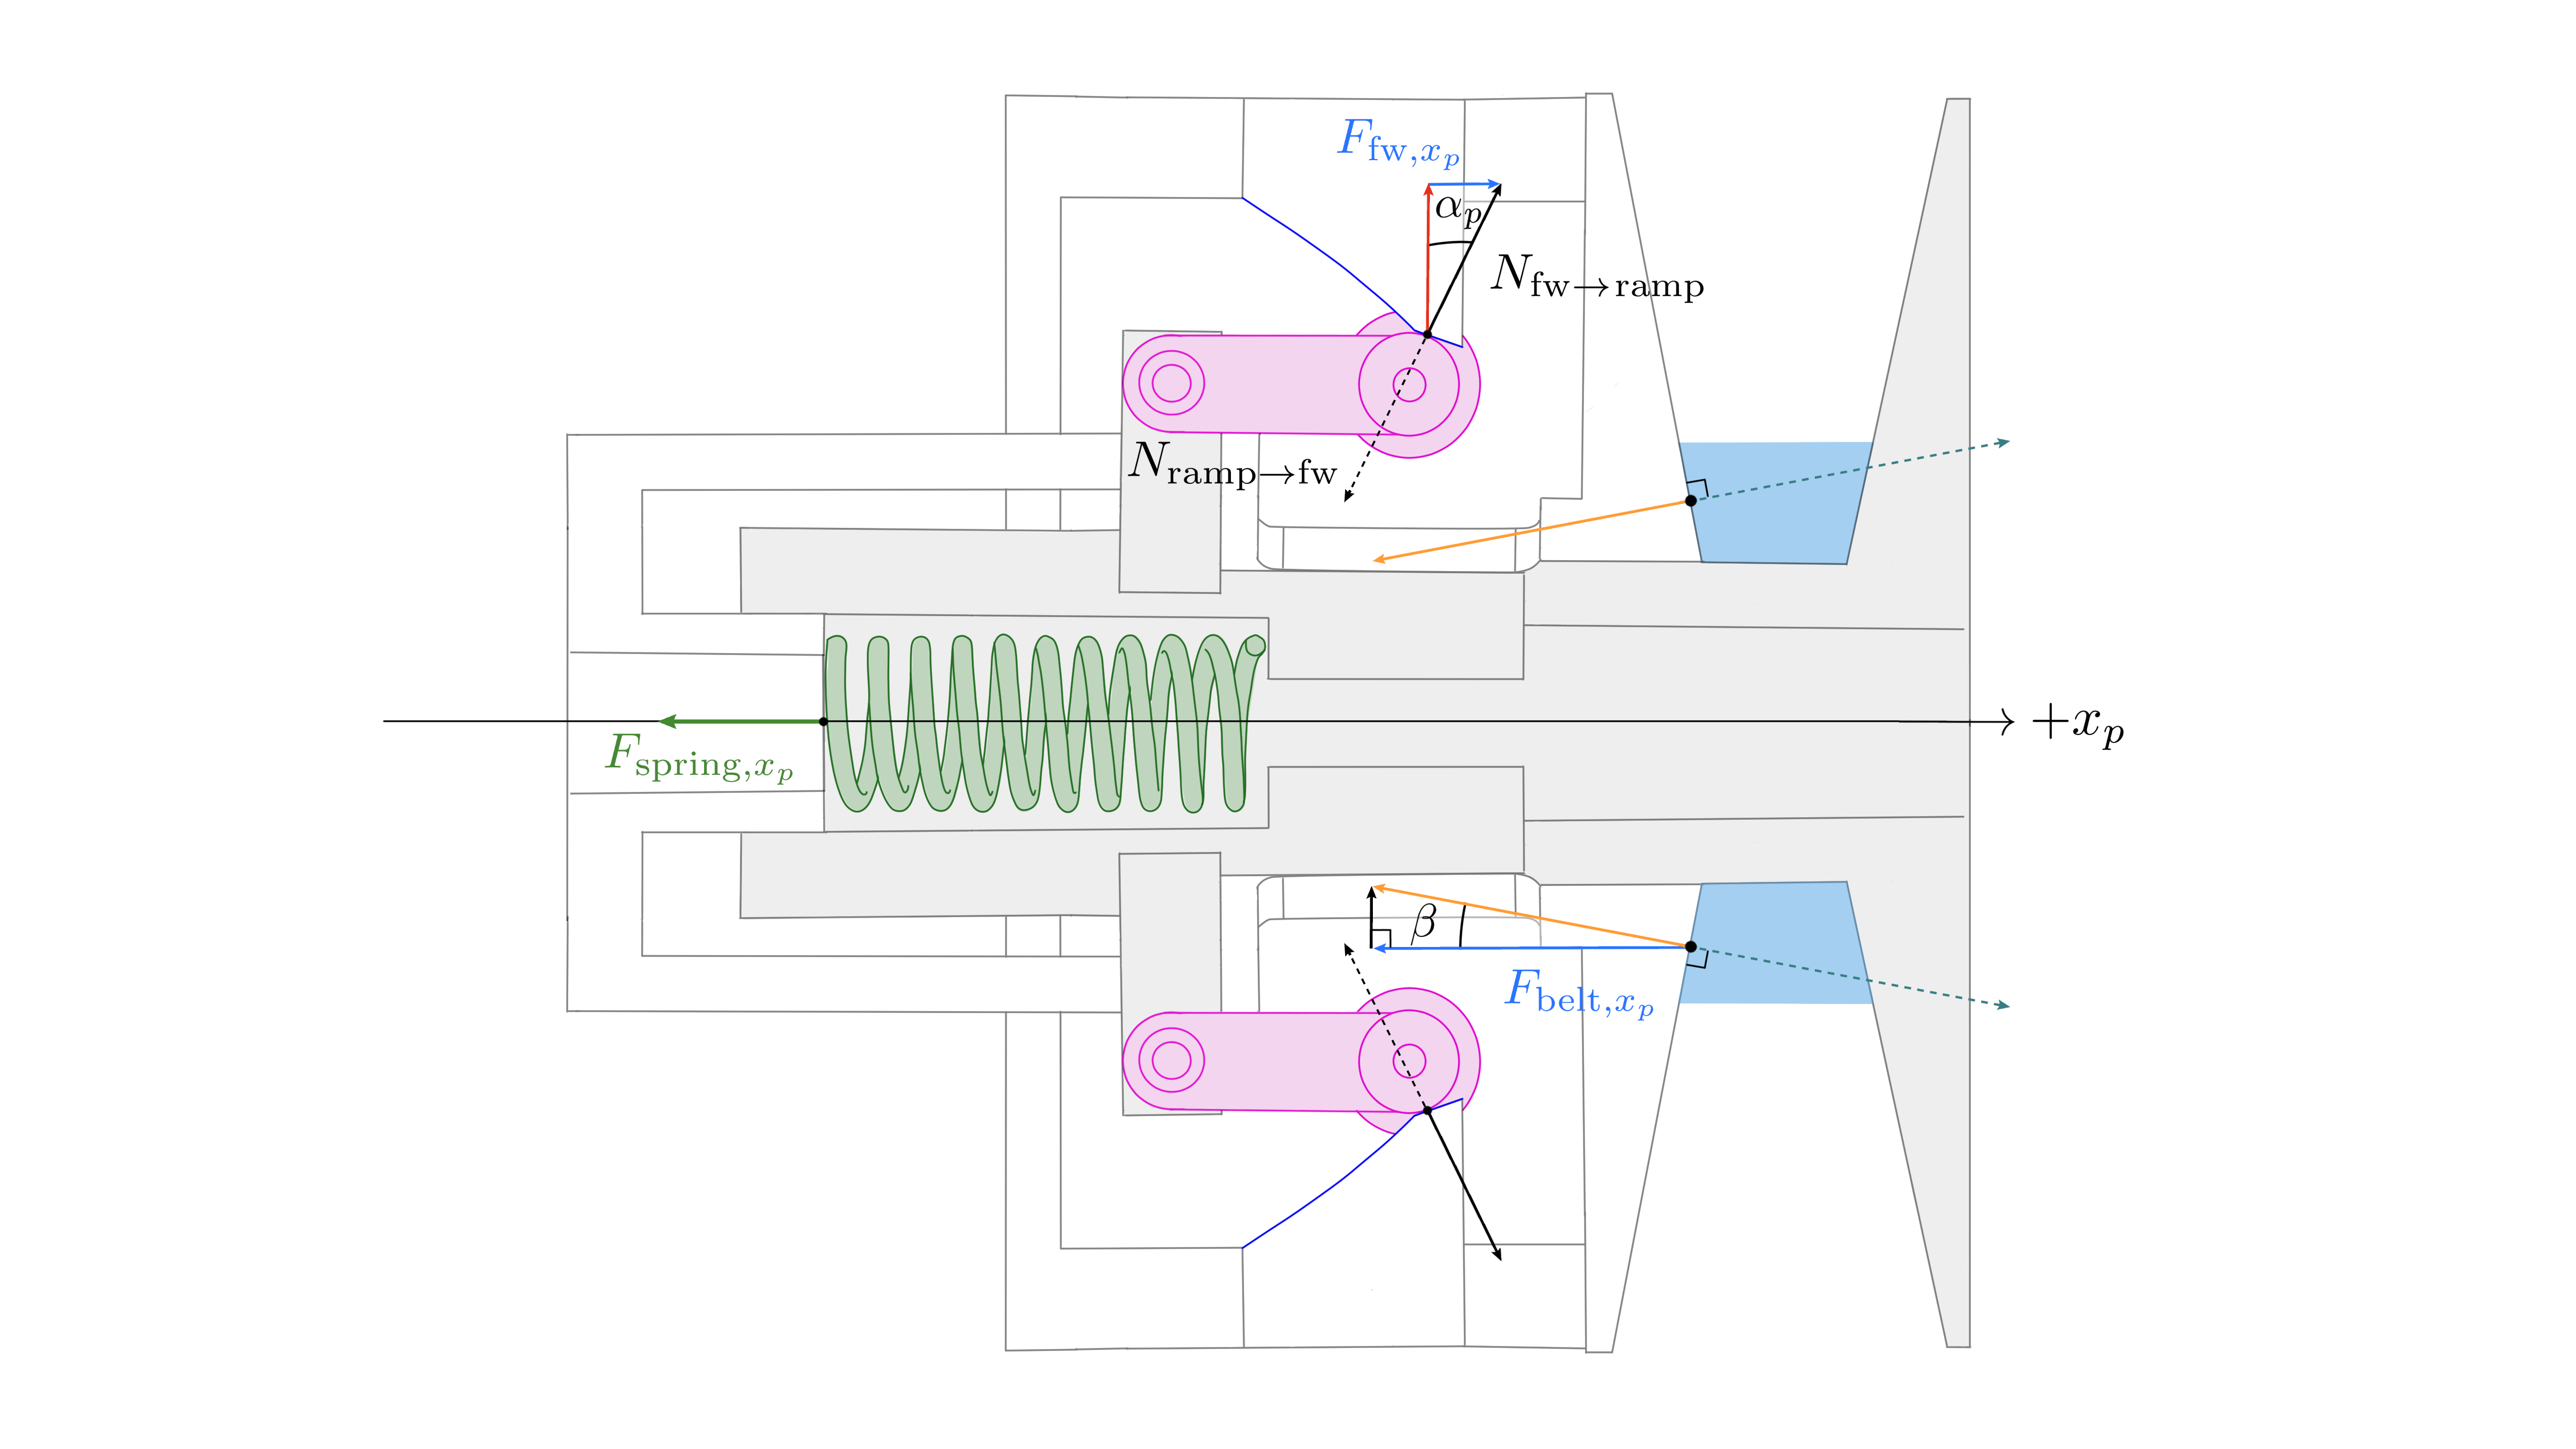
\includegraphics[width=\linewidth]{./figures/actuation/primary_axial.png}
    \caption{Axial free-body diagram of the primary movable assembly (unshaded). The
    symmetric sides of the cross-section are used to show the
    flyweight--ramp and belt--sheave force resolutions separately. Dotted
    arrows show the equal-and-opposite forces on the flyweight and belt,
    with \(F_{\mathrm{clamp}}\) indicating the movable sheave's squeeze on
    the belt.}
    \label{fig:primary_clamping_mechanism}
\end{figure}

As established in \Cref{sec:geometry}, positive \(x_p\) closes the primary.
Let \(m_p\) be the total mass of the movable sheave, ramp carrier, and every
other component that translates rigidly with them. The three axial forces
shown in \Cref{fig:primary_clamping_mechanism} are:

\begin{itemize}
    \item \(F_{\mathrm{fw},x_p}\), the closing force delivered to the
          ramp carrier by the flyweight contacts;
    \item \(F_{\mathrm{spring},x_p}\), the opening force exerted by the primary
          spring; and
    \item \(F_{\mathrm{belt},x_p}\), the opening force exerted by the belt on
          the movable face.
\end{itemize}

Newton's second law along the shaft is therefore

\begin{equation}
    m_p\ddot x_p
    =
    F_{\mathrm{fw},x_p}
    -
    F_{\mathrm{spring},x_p}
    -
    F_{\mathrm{belt},x_p}.
    \label{eq:primary_movable_sheave_balance}
\end{equation}

This free body tells us exactly what remains to be found. The spring force
will follow from its compression, and the belt force from the normal reaction
on the conical face. The flyweight force is harder. It is the axial result of
a contact on a body that pivots rather than translating rigidly with the
sheave. We therefore determine \(F_{\mathrm{fw},x_p}\) first.

% --------------------------------------------------------------
\subsubsection{Force Transmitted by the Flyweights}
\label{sec:primary_flyweight_closing_force}

\paragraph{Flyweight free body}

\Cref{fig:primary_flyweight_free_body} isolates one flyweight in the
radial--axial plane fixed to the primary. The flyweight is pinned at \(P\) and
pivots about the circumferential axis through that point. Its pose is described
by \(q_f\), measured from \(+x_p\) to the body-fixed reference line shown in
the figure. At \(q_f=0\), this line is aligned with \(+x_p\); at
\(q_f=\pi/2\), it points radially outward. Increasing \(q_f\) therefore
describes the outward-pivoting direction.

\begin{figure}[H]
    \centering
    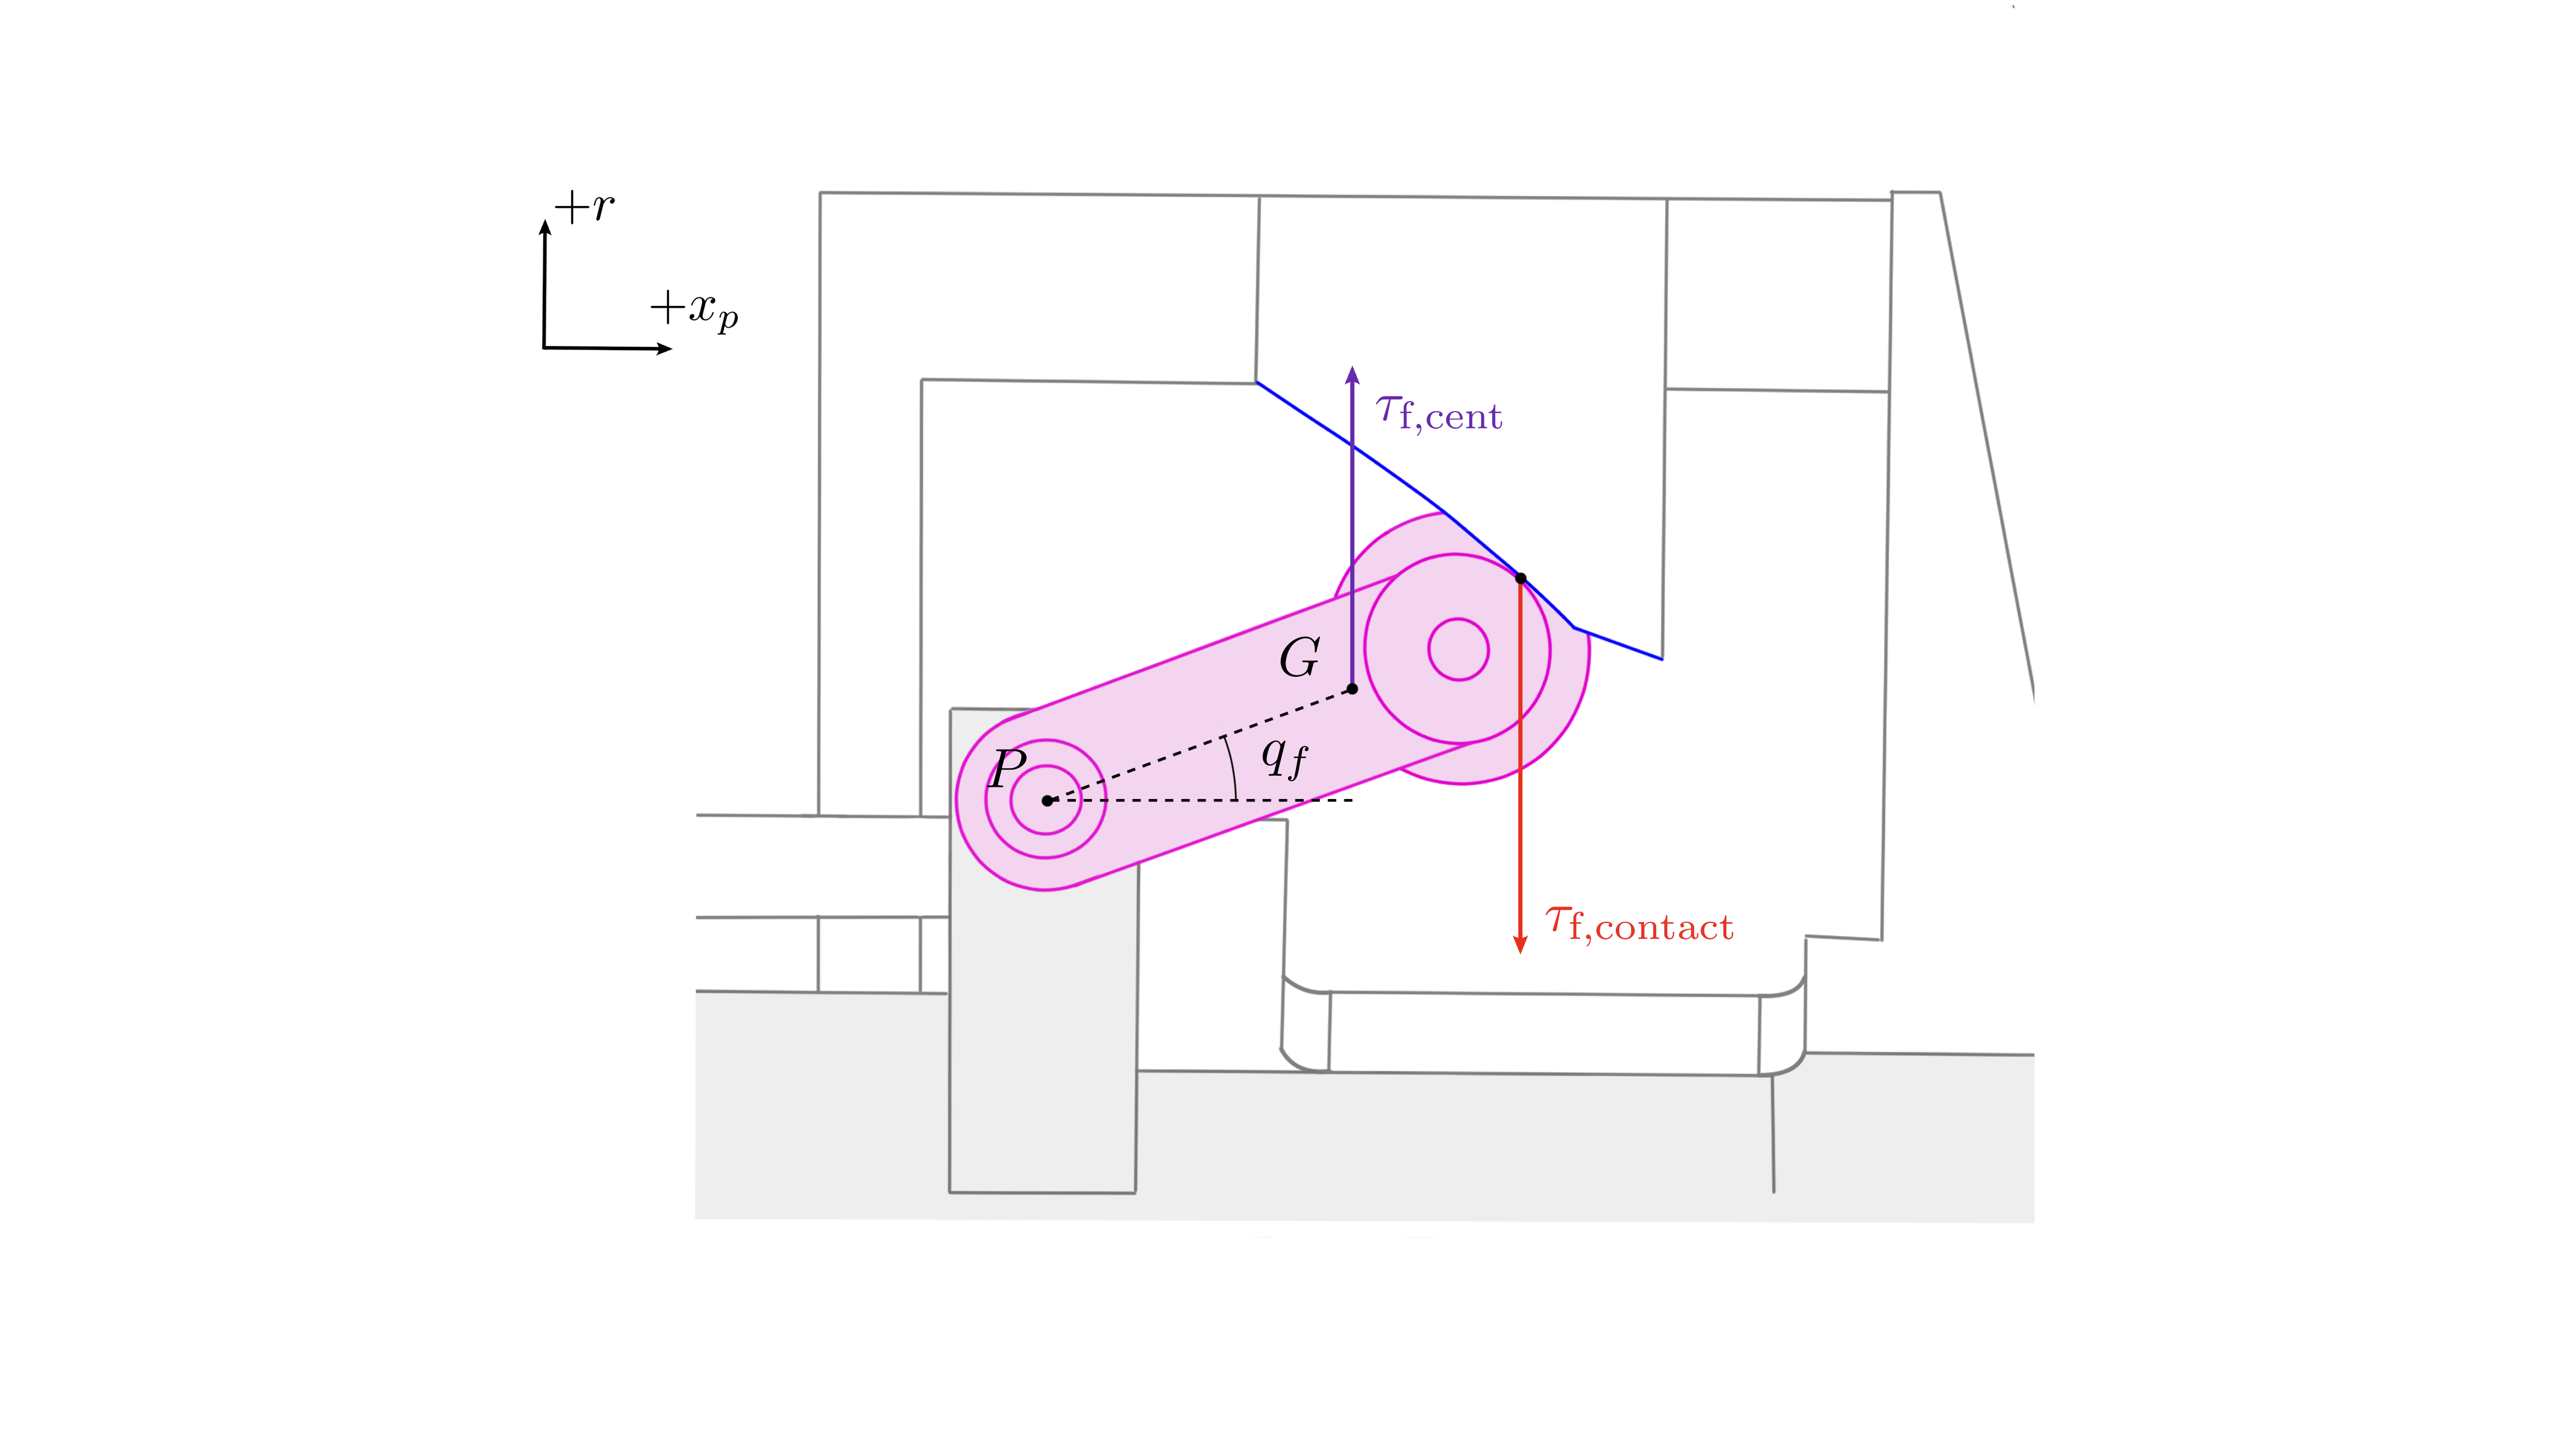
\includegraphics[width=\linewidth]{./figures/actuation/flyweight_fbd.png}
    \caption{Free body of one primary flyweight in the frame rotating with
    the primary. Centrifugal loading acts throughout the flyweight mass; the
    marked element \(A\) identifies one infinitesimal mass \(dm\) at shaft
    radius \(r_A\) and its outward load. The ramp-contact normal at \(C\) and
    the pivot reaction at \(P\) complete the force system.}
    \label{fig:primary_flyweight_free_body}
\end{figure}

As the primary rotates at \(\omega_p\), the flyweight experiences
centrifugal loading throughout its mass. Each infinitesimal element is loaded
radially outward according to its distance from the primary shaft. The marked
element \(A\) is one example: for mass \(dm\) at shaft radius \(r_A\), its
outward load is

\begin{equation}
    dF_{\mathrm{cent},A}
    =
    \omega_p^2 r_A\,dm.
    \label{eq:primary_flyweight_element_centrifugal_load}
\end{equation}

Every other element is loaded in the same way at its own shaft radius.
Together, these forces form the distributed centrifugal loading of the
flyweight.

Because the flyweight's relative motion is confined to the radial--axial
plane, the Euler and Coriolis inertial forces are circumferential and have no
moment about the circumferential pivot axis. The \(q_f\) balance therefore
depends on \(\omega_p\), but not on \(\dot\omega_p\).

Taking moments about \(P\) separates the roles of these loads. The pivot
reaction passes through \(P\) and therefore contributes no moment. The radial
lines of action of the centrifugal loads generally do not pass through
\(P\), so together they produce a moment in the direction of increasing
\(q_f\). The ramp normal produces the opposing moment.

The figure shows one flyweight, whereas the primary contains a symmetric set
whose members follow the same \(q_f\). Let
\(\tau_{f,\mathrm{cent}}\) and \(\tau_{f,\mathrm{contact}}\) denote the
respective magnitudes of the centrifugal and contact moments summed over this
complete set. Since their shared coordinate \(q_f\) is a rotation about the
flyweight pivots, let \(I_f\) denote the sum of each flyweight's mass moment
of inertia about its own pivot axis. With positive moment defined in the
direction of increasing \(q_f\), rotational Newton's second law gives
\nopagebreak[4]

\begin{equation}
    \tau_{f,\mathrm{cent}}
    -
    \tau_{f,\mathrm{contact}}
    =
    I_f\ddot q_f.
    \label{eq:primary_flyweight_moment_balance}
\end{equation}

\paragraph{Mechanism geometry}

The moment balance is written in the flyweight coordinate \(q_f\), whereas
the force required by the movable-sheave balance must be expressed through
the axial coordinate \(x_p\). The ramp geometry connects the two: each sheave
position fixes the corresponding flyweight pose.

The centrifugal moment in
\Cref{eq:primary_flyweight_moment_balance} comes from the distributed loading
shown in the figure, so its value depends on how the complete flyweight mass
is distributed about the primary shaft. The marked element \(A\) contributes
\(r_A^2\,dm\) to the mass moment of inertia about that shaft. Adding the
corresponding contributions from every element of every flyweight gives the
complete shaft-axis inertia \(J_{f,p}\). Since \(x_p\) fixes the flyweight
pose, it fixes every element's shaft radius and therefore fixes \(J_{f,p}\).
This shaft-axis inertia should not be confused with the pivot-axis inertia
\(I_f\) in \Cref{eq:primary_flyweight_moment_balance}, which is constant for
rigid flyweights.

The mechanism therefore supplies two configuration maps:

\begin{equation}
    q_f=q_f(x_p),
    \qquad
    J_{f,p}=J_{f,p}(x_p).
    \label{eq:primary_flyweight_geometry_maps}
\end{equation}

Together with the constant \(I_f\), these maps abstract the physical geometry
of the flyweight mechanism into the quantities required by the general force
balance.

\begin{remarkbox}[Remark (Constructing the flyweight maps)]
The mechanism-specific construction is not carried out here.
\Cref{sec:primary_flyweight_geometry_examples} works through two common
flyweight arrangements, showing how their geometry and mass distribution
produce \(q_f(x_p)\), \(J_{f,p}(x_p)\), and \(I_f\).
\end{remarkbox}

With these mechanism properties specified, the remaining task is to express
the two moments and \(\ddot q_f\) in
\Cref{eq:primary_flyweight_moment_balance} through the primary motion. We
begin with the moments.

Both could be found by resolving the forces and constructing their moment arms
for the specific flyweight geometry. A more convenient approach is equivalent
virtual work. Hold the mechanism at its current position and imagine a small
compatible motion. During this motion, a moment \(\tau_f\) acting through
\(dq_f\) performs the work

\begin{equation}
    \tau_f\,dq_f = \delta W_f.
\end{equation}

We can therefore find each moment by calculating the work of its underlying
load during the same motion.

For the centrifugal loading, at fixed instantaneous angular speed, the work
associated with a change \(dJ\) in shaft-axis inertia is
\(\tfrac{1}{2}\omega^2\,dJ\). Applying this relation to the flyweights gives

\begin{equation}
    \tau_{f,\mathrm{cent}}\,dq_f
    =
    \delta W_{f,\mathrm{cent}}
    =
    \frac{1}{2}\omega_p^2\,dJ_{f,p}.
    \label{eq:primary_centrifugal_work}
\end{equation}

For the contact moment, the corresponding work is the force--displacement
work \(F\,d\ell\). The movable sheave moves axially through \(dx_p\), so only
the axial component of the ramp-contact force performs work. This component
is \(F_{\mathrm{fw},x_p}\), the closing force introduced by the movable-sheave
free body, and its work is therefore \(F_{\mathrm{fw},x_p}\,dx_p\). Under
\AssRef{assump:ideal_actuator_mechanics}, the ramp contact is treated as an
ideal frictionless constraint, so no work is dissipated at the contact. The
work of the contact moment therefore appears entirely as axial work on the
movable assembly. Using the positive magnitudes defined above,

\begin{equation}
    \tau_{f,\mathrm{contact}}\,dq_f
    =
    \delta W_{f,\mathrm{contact}}
    =
    F_{\mathrm{fw},x_p}\,dx_p.
    \label{eq:primary_contact_work}
\end{equation}

\paragraph{Flyweight acceleration}

The two moment terms are now written in forms that can be returned to the
rotational balance. Its remaining term is the flyweight angular acceleration.
Ramp contact makes this acceleration a consequence of the sheave motion rather
than an independent state. Since the contact geometry already gives \(q_f\) as
a function of \(x_p\), its angular velocity is

\begin{equation}
    \dot q_f
    =
    \frac{dq_f}{dx_p}\dot x_p,
    \label{eq:primary_flyweight_angular_velocity}
\end{equation}

and one more derivative gives

\begin{equation}
    \ddot q_f
    =
    \frac{dq_f}{dx_p}\ddot x_p
    +
    \frac{d^2q_f}{dx_p^2}\dot x_p^2.
    \label{eq:primary_flyweight_angular_acceleration}
\end{equation}

The second term appears when the amount of flyweight rotation required per
unit sheave travel changes along the ramp. Even at constant \(\dot x_p\), the
flyweight then changes angular speed as it moves.

\paragraph{Axial closing force}

There is now an expression for every term in the rotational balance.
Multiplying \Cref{eq:primary_flyweight_moment_balance} by \(dq_f\) and
substituting
\Cref{eq:primary_centrifugal_work,eq:primary_contact_work,%
eq:primary_flyweight_angular_acceleration} brings them together,

\begin{equation}
    \frac{1}{2}\omega_p^2dJ_{f,p}
    -
    F_{\mathrm{fw},x_p}dx_p
    =
    I_f
    \left(
        \frac{dq_f}{dx_p}\ddot x_p
        +
        \frac{d^2q_f}{dx_p^2}\dot x_p^2
    \right)
    dq_f.
    \label{eq:primary_flyweight_moment_balance_axial}
\end{equation}

Rearranging for the force transmitted to the movable sheave gives

\begin{equation}
\boxed{
\begin{aligned}
    F_{\mathrm{fw},x_p}
    ={}&
    \frac{1}{2}\omega_p^2\frac{dJ_{f,p}}{dx_p}
    -
    I_f
    \left(\frac{dq_f}{dx_p}\right)^2
    \ddot x_p
    \\
    &-
    I_f
    \frac{dq_f}{dx_p}
    \frac{d^2q_f}{dx_p^2}
    \dot x_p^2.
\end{aligned}
}
    \label{eq:primary_flyweight_axial_force}
\end{equation}

The result now has the form required by the movable-sheave free body. The first
term is the centrifugal drive and therefore uses the shaft-axis property
\(J_{f,p}\). The final two terms arise from acceleration about the flyweight
pivots and therefore use the pivot-axis property \(I_f\): the first reflects
\(\ddot x_p\) through the motion ratio, while the second appears when that
motion ratio changes with position.

\begin{remarkbox}[Remark (Admissible flyweight maps)]
The completed force law uses \(q_f''(x_p)\) and \(J_{f,p}'(x_p)\), while the
selected coordinate directions require primary closure to correspond to
outward flyweight rotation. Over the admissible shift range, the supplied
mechanism maps must therefore satisfy
\[
    q_f\in C^2,
    \qquad
    J_{f,p}\in C^1,
    \qquad
    0<
    \frac{dq_f}{dx_p}
    <\infty.
\]
These are requirements on the fitted or constructed maps, not additional
equations of motion.
\end{remarkbox}

The one-sided flyweight contact can transmit compression but not tension, so
the force predicted by \Cref{eq:primary_flyweight_axial_force} must satisfy
\(F_{\mathrm{fw},x_p}\geq0\).


% --------------------------------------------------------------
\subsubsection{Spring and Belt Forces}
\label{sec:primary_direct_forces}

Returning to the axial force balance, the two remaining forces in
\Cref{eq:primary_movable_sheave_balance} act directly on the translating
assembly.

\paragraph{Primary spring}

Let \(k_p\) be the spring stiffness and \(x_{p,\mathrm{pre}}\) its installed
compression when the primary is open at \(x_p=0\). Closing the sheave by
\(x_p\) adds the same amount of compression, so the spring opening force is

\begin{equation}
    F_{\mathrm{spring},x_p}
    =
    k_p\left(x_{p,\mathrm{pre}}+x_p\right).
    \label{eq:primary_spring_force}
\end{equation}

\paragraph{Belt reaction}

Let \(N_p\) be the total integrated normal load over both primary sheave
faces. This load is coupled to the belt and the secondary balance, so it
remains an unknown at this stage. Under
\AssRef{assump:symmetric_face_sharing}, the movable face carries one half of
this total load. Its normal is inclined by the sheave half-angle
\(\beta\) from the axial direction, so the opening force on the movable face is

\begin{equation}
    F_{\mathrm{belt},x_p}
    =
    \frac{N_p}{2}\cos\beta.
    \label{eq:primary_belt_axial_reaction}
\end{equation}

% --------------------------------------------------------------
\subsubsection{Completed Primary Balance}
\label{sec:completed_primary_balance}

Each force in the original free body now has a mechanism-level expression.
Substitute
\Cref{eq:primary_flyweight_axial_force,eq:primary_spring_force,%
eq:primary_belt_axial_reaction} into
\Cref{eq:primary_movable_sheave_balance} and collect the terms multiplying
\(\ddot x_p\):

\begin{equation}
\boxed{
\begin{aligned}
    \left[
        m_p
        +
        I_f
        \left(\frac{dq_f}{dx_p}\right)^2
    \right]\ddot x_p
    ={}&
    \frac{1}{2}\omega_p^2\frac{dJ_{f,p}}{dx_p}
    \\
    &-
    I_f
    \frac{dq_f}{dx_p}
    \frac{d^2q_f}{dx_p^2}
    \dot x_p^2
    \\
    &-
    k_p\left(x_{p,\mathrm{pre}}+x_p\right)
    -
    \frac{N_p}{2}\cos\beta.
\end{aligned}
}
    \label{eq:completed_primary_axial_balance}
\end{equation}

The flyweights now appear through the same two axes introduced by their free
body. Rotation about the primary shaft, described by \(J_{f,p}\), provides
the speed-dependent closing drive. Rotation about the flyweight pivots,
described by \(I_f\), adds to the inertia that the axial motion must
accelerate. If the motion ratio \(dq_f/dx_p\) changes along the ramp, the
flyweights also accelerate even when \(\dot x_p\) is constant, producing the
term proportional to \(\dot x_p^2\). The spring and belt forces act directly
on the movable assembly and oppose closure exactly as shown in the first free
body.

This is the primary axial equation of motion. It states how the
flyweight action is divided among spring compression, belt loading, and
acceleration of the translating and pivoting hardware.

\subsubsection{Point-Mass Limit and Relation to Existing Models}
\label{sec:primary_classical_limit}

The general force law becomes the familiar classical actuator model when the
distributed flyweight mass is collapsed to its centre of mass and the
flyweight's pivot dynamics are neglected. Let \(m_f\) be the total mass of
the symmetric flyweight set and let \(r_f(x_p)\) be the common instantaneous
centre-of-mass radius. Under the point-mass assumption, the shaft-axis inertia
reduces to

\begin{equation}
    J_{f,p}
    =
    m_f r_f^2.
    \label{eq:primary_flyweight_lumped_inertia}
\end{equation}

Substituting this point-mass inertia into the centrifugal term of
\Cref{eq:primary_flyweight_axial_force}, while omitting the pivot-acceleration
terms, gives

\begin{equation}
    F_{\mathrm{fw},x_p}^{\mathrm{pm}}
    =
    m_f r_f\omega_p^2
    \frac{dr_f}{dx_p}.
    \label{eq:primary_flyweight_point_mass_limit}
\end{equation}

This is the familiar point-mass result. The factor
\(m_f r_f\omega_p^2\) is the total centrifugal loading, while
\(dr_f/dx_p\) is the local radial-to-axial motion ratio that converts that
loading into sheave force. The path need not be straight, and its motion ratio
need not be constant. A sliding mass on a straight ramp is one simple case;
for a pivoted flyweight, \(r_f(x_p)\) instead follows from the flyweight pose
and its mass geometry.

If the movable sheave is also in axial equilibrium, the point-mass actuator
force balances the opening forces from the spring and belt:

\begin{equation}
    m_f r_f\omega_p^2
    \frac{dr_f}{dx_p}
    =
    k_p\left(x_{p,\mathrm{pre}}+x_p\right)
    +
    \frac{N_p}{2}\cos\beta.
    \label{eq:primary_classical_equilibrium}
\end{equation}

This reduction appears directly in the quasi-static model of
\citet{Messick2018}. Their three wedge-shaped flyweights slide along linear
ramps without changing orientation. Measured CAD geometry supplies the
centre-of-mass radius and the radial-to-axial displacement ratio, giving a
force of the same form as
\Cref{eq:primary_flyweight_point_mass_limit}. Friction is neglected, and the
resulting primary force is supplied to the belt model as a boundary condition;
shifting is treated as a sequence of equilibrium configurations rather than a
time-dependent response. \citet{ArangoMunoz2020} use the same
instantaneous force conversion to construct both sliding-weight ramps and
pivoted flyweight-cam profiles. Their contact geometry is designed so that
the available centrifugal force supplies the required clamping force through
the local mechanical advantage.

Other treatments retain more of the contact geometry while keeping the same
instantaneous-equilibrium closure. \citet{KimEtAl2002} resolve the two
contacts of a centrifugal roller and include contact friction when converting
roller centrifugal force into driver thrust. The current roller radius and
contact angles vary with ratio, but no roller acceleration enters the thrust
equation. \citet{Skinner2020} resolve a flyweight, its supporting link, and
the ramp reactions in a complete free body, including the centrifugal loading
of both the flyweight and the link. In the present notation, those separate
mass contributions could be collected in \(J_{f,p}(x_p)\). Skinner's
derivation therefore retains a substantially richer equilibrium force path
than a single fixed ramp factor, but still closes the flyweight system by
force equilibrium at each configuration.

Despite their different levels of geometric detail, none of these actuator
relations includes the acceleration of the flyweight mechanism. Messick does
not model shift time, Skinner solves algebraically for the speed required at
each configuration, and Kim places the time dependence in a separate
experimentally identified first-order ratio law, using different fitted
coefficients for upshift and downshift. Conversely, the transient belt model
of \citet{Ballew2015} imposes primary axial force through a controller rather
than resolving the mechanical actuator. Across these examples, transient
shift motion is therefore obtained without returning the flyweights' own
acceleration to the primary axial balance.

The distinction of the present formulation is therefore not that it can
describe a curved ramp or a detailed flyweight shape; the equilibrium models
above can already retain substantial geometric detail. Here, the complete
mass distribution enters through \(J_{f,p}(x_p)\), so the centrifugal drive is
not restricted to a centre-of-mass point model. More importantly, the
flyweight moment balance is not closed at instantaneous equilibrium. Mapping
\(I_f\ddot q_f\) into \(x_p\) produces both the reflected pivot inertia and
the changing-motion-ratio term in
\Cref{eq:completed_primary_axial_balance}. Consequently, the flyweight drive,
spring force, belt reaction, translating mass, and pivoting mass all determine
the same shift acceleration rather than being divided between an equilibrium
actuator law and a separate shift-response model. No equivalent explicit
reflection of the flyweights' pivoting inertia was identified in the reviewed
mechanically actuated rubber-belt CVT formulations.

This extension does not retain every effect represented in the earlier
models. Structural deformation is excluded by \AssRef{assump:rigid_hardware},
while \AssRef{assump:ideal_actuator_mechanics} treats the ramp contact as an
ideal constraint rather than resolving its tribology or local compliance. The
roller-contact friction retained by \citet{KimEtAl2002}, for example,
therefore lies outside the present force law; roller spin and contact compliance
are likewise not resolved. The added fidelity is in the coupled
mechanism dynamics, not in frictional or compliant contact detail.


\subsection{Secondary Movable-Sheave Balance}
\label{sec:secondary_movable_sheave_balance}

While the primary closes mainly in response to rotational speed, the secondary is
torque reactive: torque transmitted through the pulley can also increase the
axial force clamping the belt.

To see how, begin with the two secondary sheaves rotationally disconnected.
The fixed sheave rotates with the secondary shaft. The movable sheave can slide
along that shaft and rotate relative to the fixed sheave. Because the belt
contacts the two faces separately, it applies torque to each body. With no
connection between them, the two bodies can accelerate differently and rotate
relative to one another.

Now place a pin on the movable sheave in a straight slot running along the
shaft. The movable sheave remains free to slide, but the pin prevents relative
rotation. Whenever the two sheaves tend to rotate differently, the pin presses
against the side of the slot and a normal reaction develops. Because the slot
is axial, this normal acts entirely in the circumferential direction. It
transfers torque between the sheaves but produces no axial force.

A helix is the same slot tilted around the shaft. The contact normal remains
perpendicular to the slot surface, but now has both circumferential and axial
components. The circumferential component continues to couple the rotational
motion of the sheaves, while the axial component acts on the movable sheave.
Relative rotation is therefore allowed only when accompanied by axial travel
along the helix.

These three cases and their contact reactions are compared in
\Cref{fig:secondary_constraint_progression}.

\begin{figure}[H]
    \centering
    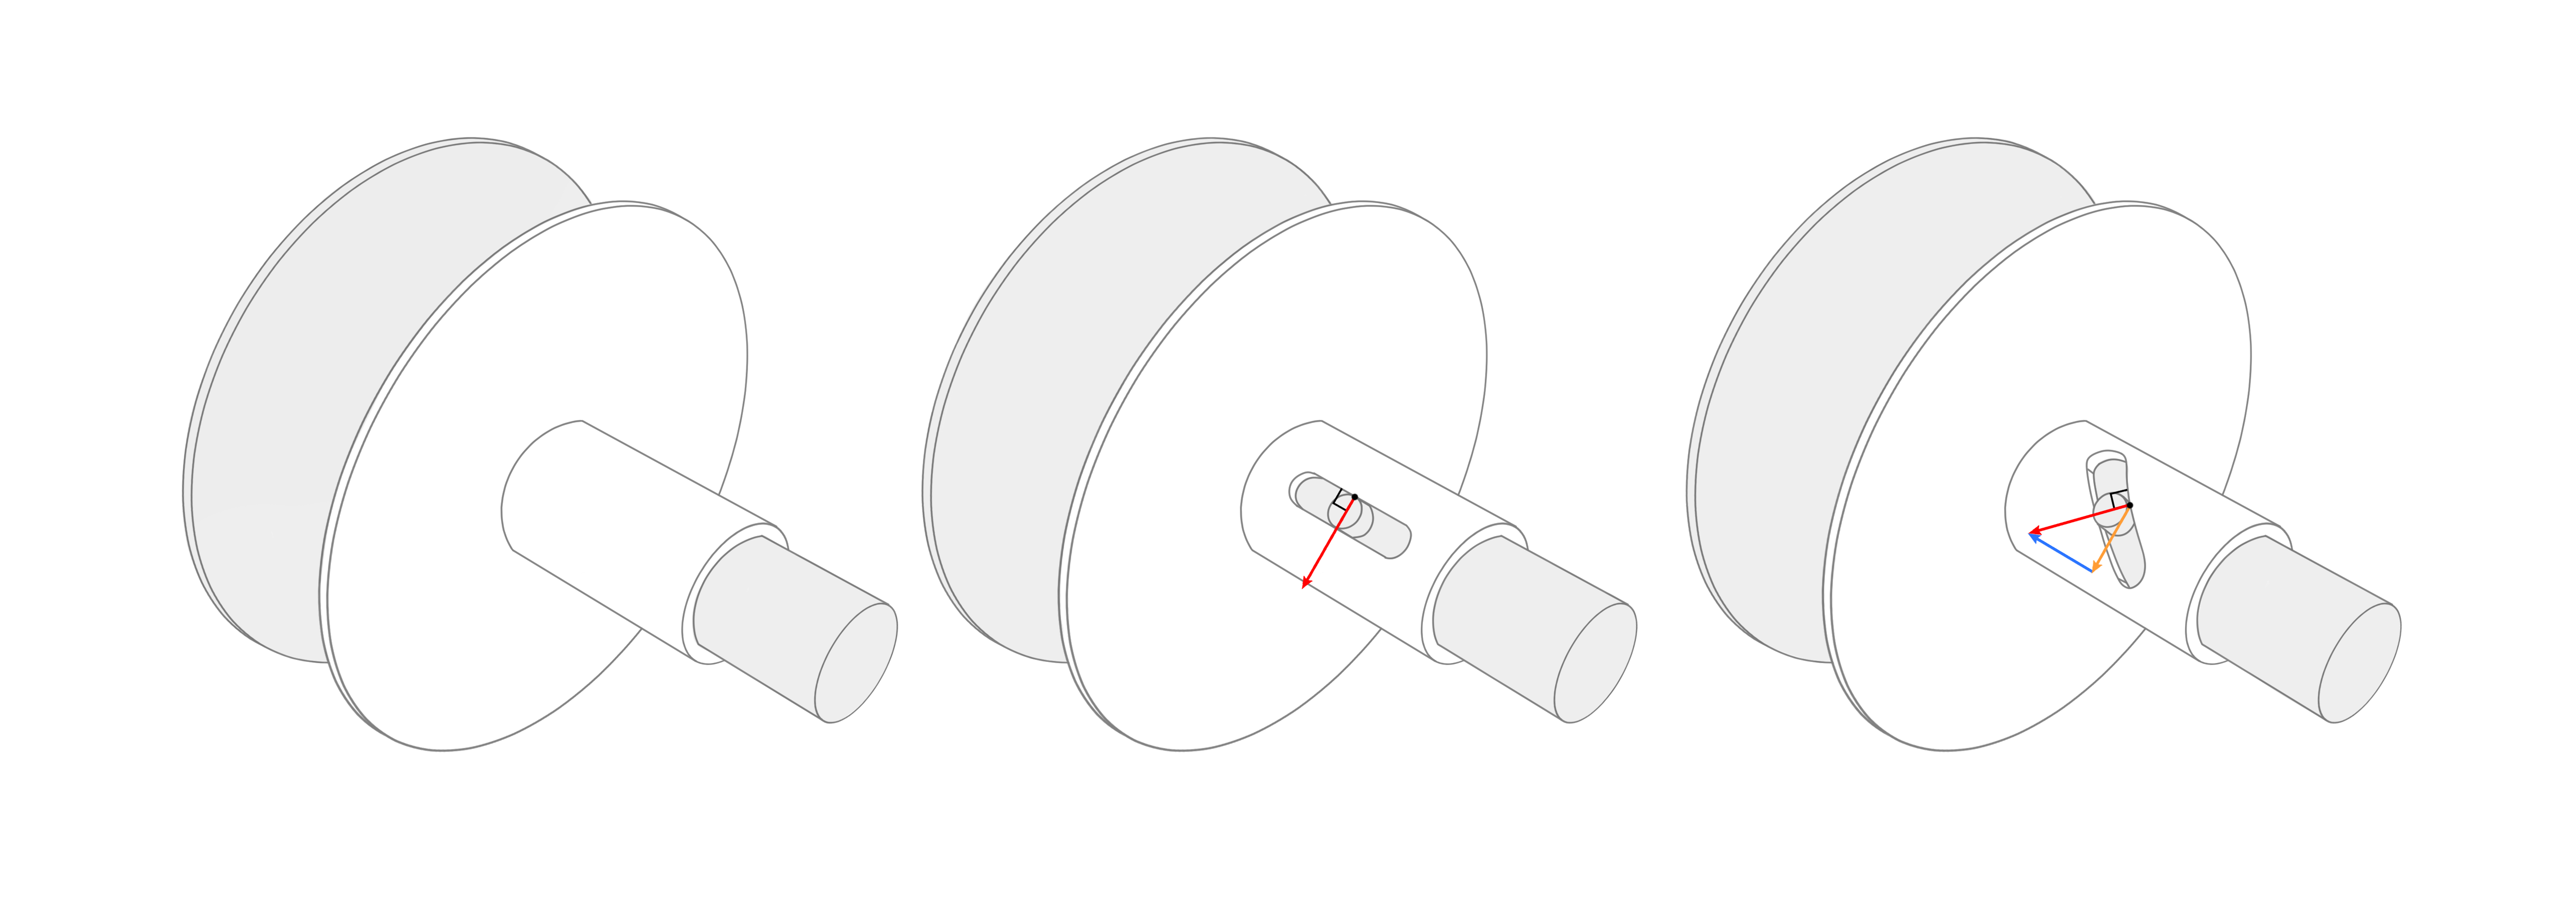
\includegraphics[width=\linewidth]{./figures/actuation/helical_slot.png}
    \caption{How the helix creates torque-reactive axial loading. With no
    connection, the two sheaves may rotate independently. A straight axial slot
    couples their rotation through a purely circumferential reaction; inclining
    the slot adds an axial component to that same reaction, coupling relative
    rotation to axial travel.}
    \label{fig:secondary_constraint_progression}
\end{figure}

If the axial component of the helix reaction is balanced by the other axial
loads, the movable sheave remains at
its current position. Its relative angle then remains fixed, and the two
sheaves rotate together with the shaft. If the axial loads do not balance, 
their resultant accelerates the movable sheave along the helix, and it 
rotates by the amount required by the slot geometry.

In the actual secondary, the belt and spring load this mechanism. The belt
applies torque to the two sheave faces separately. The secondary spring is
installed both compressed and twisted: its torsional preload tends to rotate
the movable sheave relative to the fixed sheave, while its axial compression
pushes the movable sheave toward closure. The torsional action loads the
helix; the axial action enters the movable-sheave balance directly.

The axial free body gives the target for the derivation.

% --------------------------------------------------------------
\subsubsection{Axial Free Body}
\label{sec:secondary_axial_free_body}

\Cref{fig:secondary_axial_free_body} isolates the movable assembly in the
axial direction.

\begin{figure}[H]
    \centering
    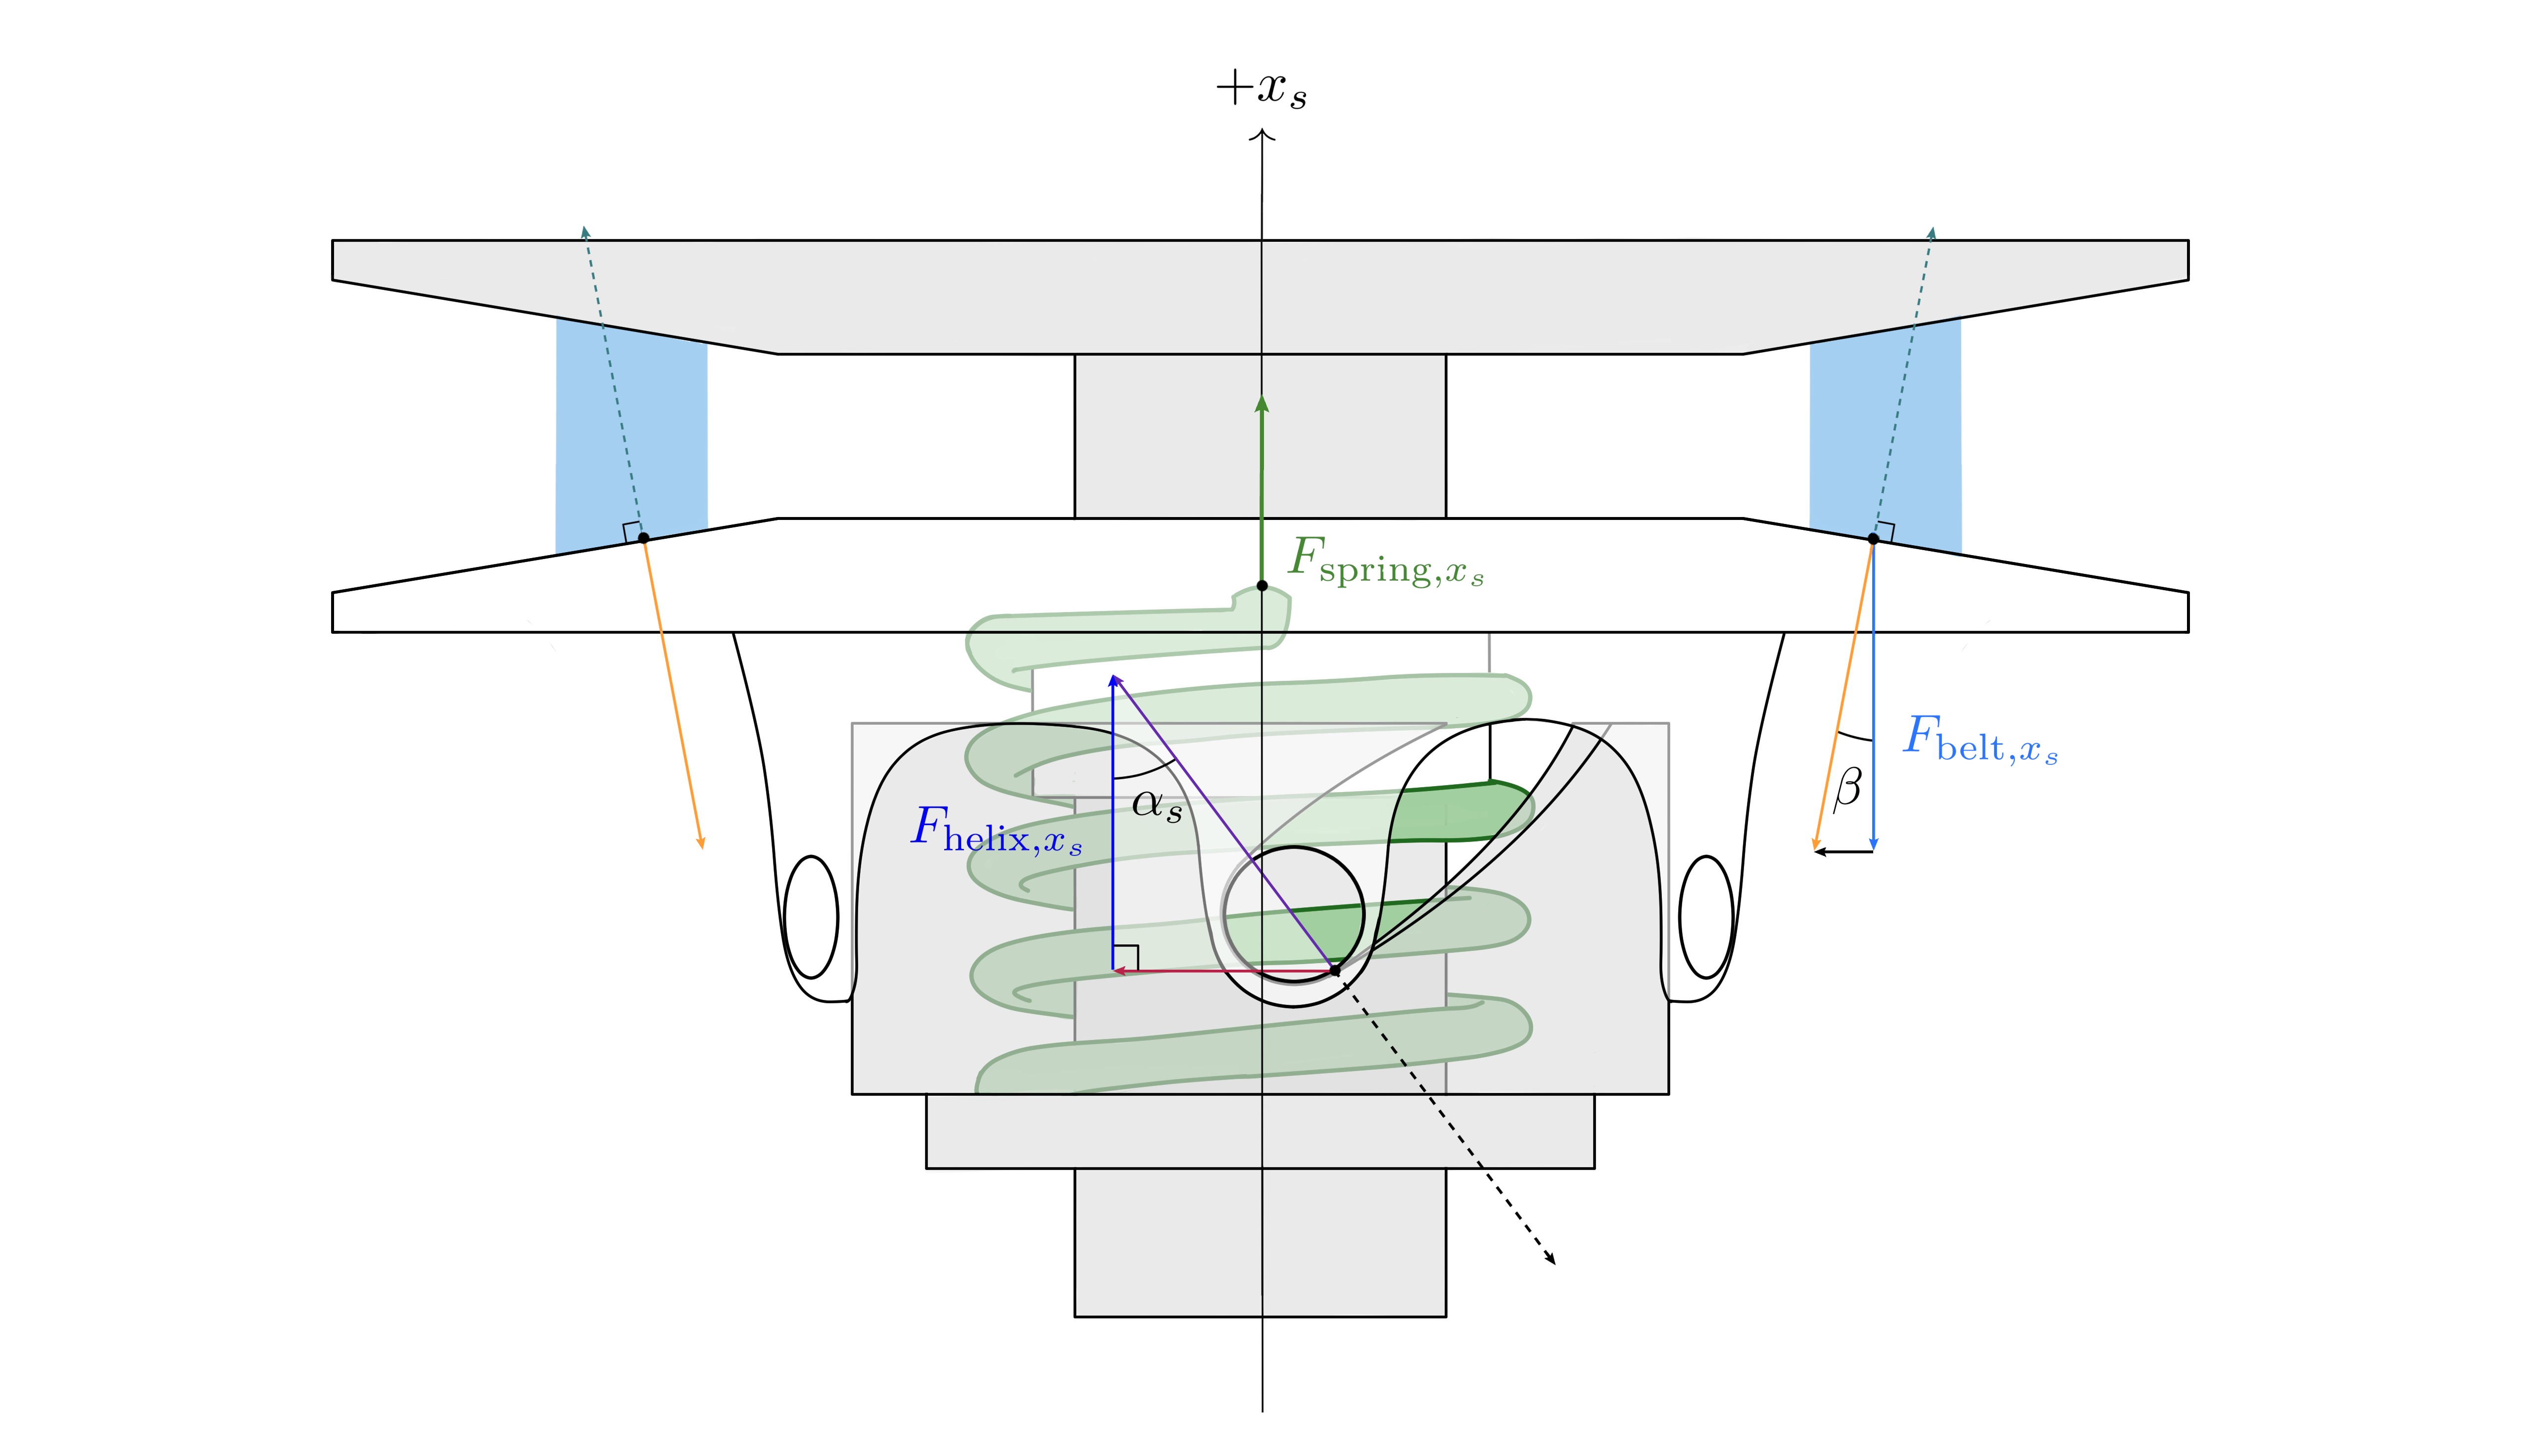
\includegraphics[width=\linewidth]{./figures/actuation/secondary_axial.png}
    \caption{Axial free body of the complete movable secondary assembly. The
    axial spring force and belt reaction act directly on the translating
    assembly, while the secondary's torque-reactive behaviour enters through the
    pin--helix force \(F_{\mathrm{helix},x_s}\).}
    \label{fig:secondary_axial_free_body}
\end{figure}

Let \(m_s\) be the mass of the movable sheave and every component that
translates rigidly with it. Three axial loads act on this assembly. The
pin--helix contact contributes the signed force
\(F_{\mathrm{helix},x_s}\). The compressed spring pushes the movable sheave
toward the fixed sheave in \(+x_s\). The belt pushes the two sheave faces
apart, so its reaction on the movable face acts in \(-x_s\), just as on the
primary. Newton's second law therefore gives

\begin{equation}
    m_s\ddot x_s
    =
    F_{\mathrm{helix},x_s}
    +F_{\mathrm{spring},x_s}
    -F_{\mathrm{belt},x_s}.
    \label{eq:secondary_movable_sheave_balance}
\end{equation}

This free body makes the remaining task clear. The direct spring and belt
forces follow from compression and contact geometry. The helix force does
not: the tilted slot has established that an axial reaction exists, but not
its magnitude or sign. Because the same contact reaction must also carry the
torque that constrains relative rotation, its rotational effect is resolved
first. This sets the order of the derivation:

\begin{enumerate}
    \item use the rotational balance to find the torque carried by the helix;
    \item use the helix geometry to convert that torque into axial force; and
    \item add this force to the direct spring and belt loads in the axial
    balance.
\end{enumerate}

% --------------------------------------------------------------
\subsubsection{Rotational Loading of the Movable Sheave}
\label{sec:secondary_rotational_loading}

As established in \Cref{sec:geometry}, \(x_s\) is measured from the open
secondary toward the fixed sheave, so \(+x_s\) closes the pulley. Let
\(\theta_s\) measure the rotation of the movable sheave relative to the fixed
sheave in the same positive rotational sense already assigned to
\(\omega_s\) (see \Cref{sec:rotational_sign}). Only the conventional torque-reactive helix orientation is
considered: as the secondary closes in \(+x_s\), the movable sheave turns
relative to the fixed sheave in \(+\theta_s\).

With these directions set, the first question is what loads the helix
circumferentially. The belt applies torque to the movable face, and the
twisted spring applies torque between the two sheaves. The pin--helix contact
supplies the torque that constrains the resulting relative motion to follow
the slot.

Our goal is to find the torque reacted at the pin--helix contact. To do so,
isolate the movable assembly and apply Newton's second law for rotation. Use
the following quantities:

\begin{itemize}
    \item \(I_{s,M}\): rotational inertia of the movable sheave and every
    component that rotates rigidly with it;
    \item \(\omega_{s,M}\): absolute angular velocity of that assembly;
    \item \(\tau_{s,M}\): signed belt torque applied to the movable face;
    \item \(\tau_{s,\mathrm{spring}}\): signed spring torque applied to the
    movable assembly; and
    \item \(\tau_{s,\mathrm{helix}}\): the contact torque at the pin--helix
    connection, produced by the circumferential component of the contact
    normal. A positive \(\tau_{s,\mathrm{helix}}\) acts on the movable
    assembly in \(-\theta_s\).
\end{itemize}

The figures show one representative pin and track. The quantities
listed above and later in this section are the
totals over the complete set of loaded pin--track contacts, so no additional
track multiplier is required.

The rotational balance is therefore

\begin{equation}
    \tau_{s,M}
    +\tau_{s,\mathrm{spring}}
    -\tau_{s,\mathrm{helix}}
    =
    I_{s,M}\dot\omega_{s,M}.
    \label{eq:secondary_movable_sheave_torque_balance}
\end{equation}

Solving for the helix torque gives

\begin{equation}
    \tau_{s,\mathrm{helix}}
    =
    \tau_{s,M}
    +\tau_{s,\mathrm{spring}}
    -I_{s,M}\dot\omega_{s,M}.
    \label{eq:secondary_reacted_helix_torque_structure}
\end{equation}

\Cref{eq:secondary_reacted_helix_torque_structure} gives the contact torque we
want, but its right-hand side still needs three relations:

\begin{itemize}
    \item the share of belt torque applied to the movable face,
    \(\tau_{s,M}\);
    \item the torque supplied by the wound spring,
    \(\tau_{s,\mathrm{spring}}\); and
    \item the absolute angular acceleration of the movable assembly,
    \(\dot\omega_{s,M}\).
\end{itemize}

The belt term follows immediately from the face-torque assumption.

\paragraph{Movable-face belt torque}

Let \(\tau_s\) be the total signed torque exerted by the belt on the secondary,
so
\(\tau_s=\tau_{s,F}+\tau_{s,M}\). Under
\AssRef{assump:symmetric_face_sharing}, the two faces receive equal torque
shares. Only the movable-face share appears in its free body:

\begin{equation}
    \tau_{s,M}
    =
    \frac{\tau_s}{2}.
    \label{eq:secondary_movable_face_belt_torque}
\end{equation}

This equal split is a reduced-contact assumption. During shift, the movable
face rotates slightly faster or slower than the fixed face. The two
belt--face contacts can therefore have different sliding conditions, so their
torques need not divide equally.

\begin{remarkbox}[Remark (Why the face-torque split can matter)]
\citet{SorgeCammalleri2011} resolve the two contacts separately and show that
the face torques can depart substantially from an equal split; distributed
tangential forces on the two faces can even act in opposite directions over
parts of the wrap. Since \(\tau_{s,M}\) enters
\Cref{eq:secondary_reacted_helix_torque_structure} directly, this is also a
potential error in the torque reacted by the helix.
\end{remarkbox}

The remaining terms both depend on the helix kinematics:
\(\dot\omega_{s,M}\) depends on how the movable sheave rotates as it shifts,
and the spring torque depends on how far that motion unwinds the spring. We
therefore derive the relation between \(x_s\) and \(\theta_s\) next.

% --------------------------------------------------------------
\subsubsection{Motion Imposed by the Helix}
\label{sec:secondary_helix_kinematics}

The helix geometry tells us how axial shift changes the relative angle of the
movable sheave. Unwrap one track from its effective cylindrical radius
\(r_h\), as seen in \Cref{fig:secondary_helix_geometry}. A small relative rotation \(d\theta_s\) moves the pin by
\(r_h\,d\theta_s\) circumferentially while the sheave moves by \(dx_s\)
axially. Let \(\alpha_s\) be the local angle of the unwrapped track, measured from the
positive circumferential direction toward the positive axial direction. For
the conventional helix orientation considered here,
\[
    0<\alpha_s<\frac{\pi}{2}.
\]

\begin{figure}[H]
    \centering
    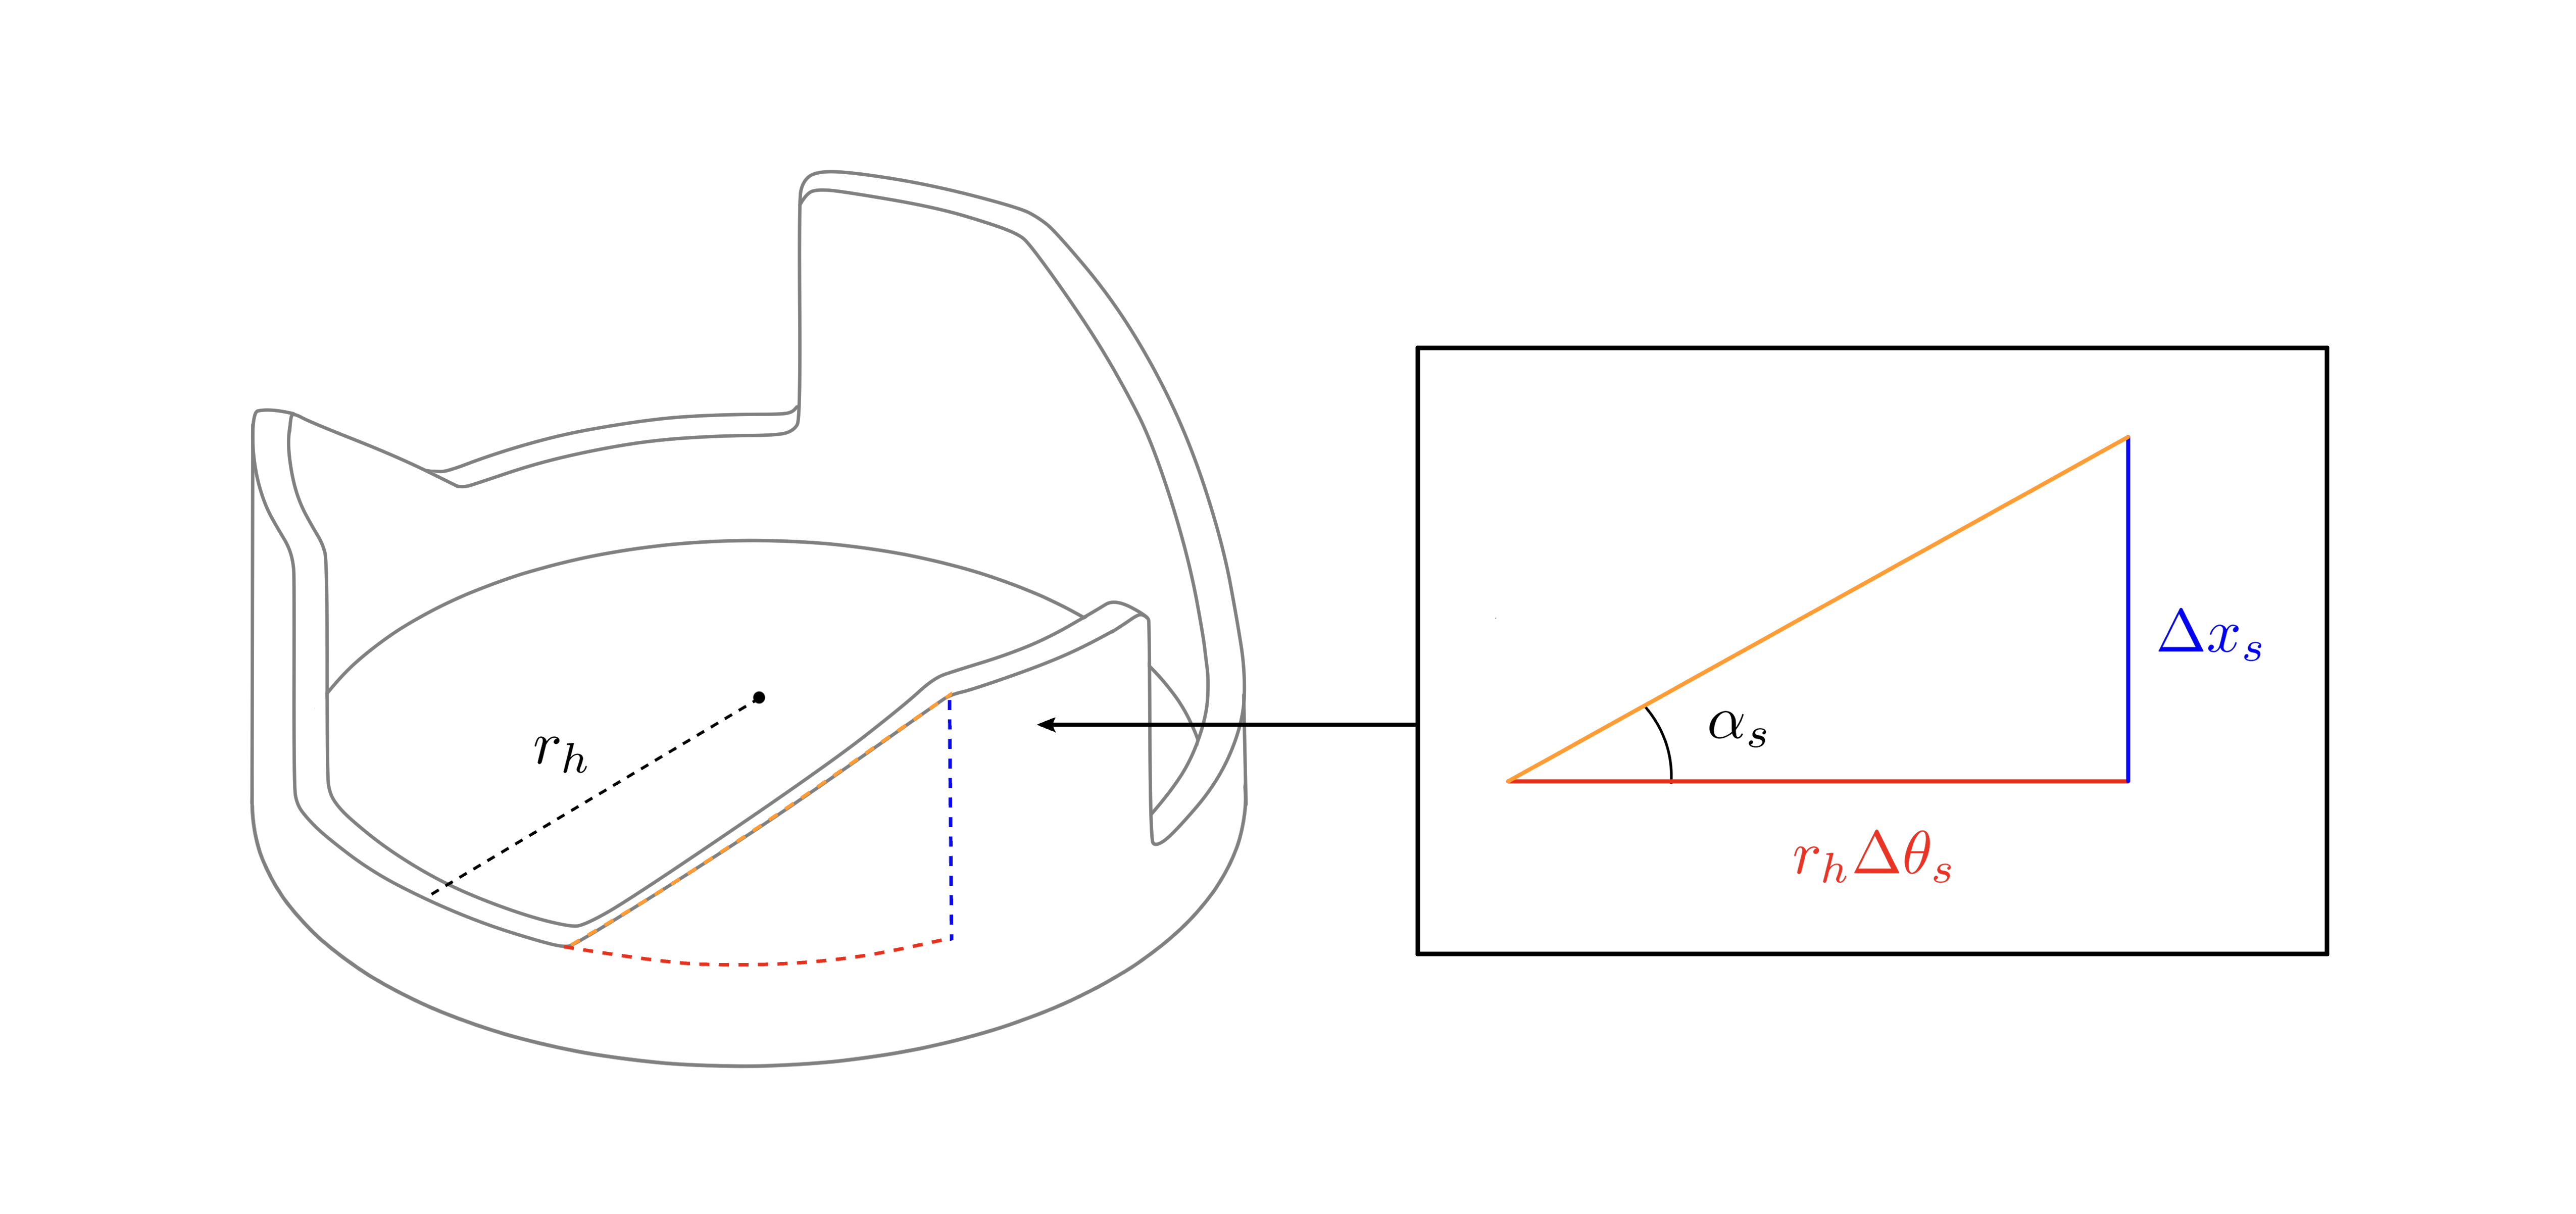
\includegraphics[width=\linewidth]{./figures/actuation/helix_unwrap.png}
    \caption{Unwrapped secondary-helix geometry. The same track angle relates
    relative rotation to axial travel and reaction torque to axial force.}
    \label{fig:secondary_helix_geometry}
\end{figure}

Taking the infinitesimal limit of the triangle in \Cref{fig:secondary_helix_geometry},

\begin{equation}
    \tan\alpha_s
    =
    \frac{dx_s}{r_h\,d\theta_s},
    \qquad
    \frac{d\theta_s}{dx_s}
    =
    \frac{1}{r_h\tan\alpha_s}.
    \label{eq:secondary_helix_motion_ratio}
\end{equation}

Thus, \(d\theta_s/dx_s\) is the relative rotation required per unit axial
travel. It is positive for the conventional helix orientation assumed here.
Returning to the straight axial slot from the opening example,
\(\alpha_s\rightarrow\pi/2\) and
\(d\theta_s/dx_s\rightarrow0\), as expected.

Taking \(\theta_s(0)=0\) at the open secondary, integrate the local motion
ratio to obtain

\begin{equation}
    \theta_s(x_s)
    =
    \int_{0}^{x_s}
    \frac{1}{r_h\tan\alpha_s(\xi)}
    \,d\xi.
    \label{eq:secondary_helix_rotation_map}
\end{equation}

\Cref{eq:secondary_helix_rotation_map} defines the helix as a function
\(\theta_s(x_s)\): for each axial position, it gives the relative angle
enforced by the track. The function need not come from a constant helix angle. Any supplied function
may be used provided it is single-valued and strictly increasing over the
admissible shift range.

\paragraph{Rotation of the movable sheave} 
We can now use this function to determine the two remaining quantities in the
rotational balance. First consider the absolute motion of the movable sheave.
The fixed sheave rotates with the secondary shaft at \(\omega_s\), while the
movable sheave also has the relative rotation \(\theta_s\):

\begin{equation}
    \omega_{s,M}
    =
    \omega_s+\dot\theta_s
    =
    \omega_s
    +
    \frac{d\theta_s}{dx_s}\dot x_s.
    \label{eq:secondary_movable_sheave_speed}
\end{equation}

Because \(\theta_s\) was defined in the same positive rotational sense as
\(\omega_s\), the relative speed enters with the plus sign shown here.
Differentiating gives the angular acceleration required by the rotational
balance:

\begin{equation}
    \dot\omega_{s,M}
    =
    \dot\omega_s
    +
    \frac{d\theta_s}{dx_s}\ddot x_s
    +
    \frac{d^2\theta_s}{dx_s^2}\dot x_s^2.
    \label{eq:secondary_movable_sheave_acceleration}
\end{equation}

The shaft acceleration \(\dot\omega_s\) remains unknown here because
\(\omega_s\) is a state of the coupled model. It is solved together with
the axial motion rather than by the helix relation alone.
The term proportional to \(\ddot x_s\) is the angular acceleration caused by
axial acceleration. The term proportional to \(\dot x_s^2\) appears only when
the motion ratio varies with position.

% --------------------------------------------------------------
\paragraph{Torsional Spring Loading}

The same helix function tells us how much the spring has unwound. Let
\(k_{s,\theta}\) be the spring's torsional stiffness and
\(\theta_{s,\mathrm{pre}}\) its signed twist at \(x_s=0\). Increasing
\(\theta_s\) reduces this twist, leaving
\(\theta_{s,\mathrm{pre}}-\theta_s(x_s)\). The resulting torque on the
movable assembly is

\begin{equation}
    \tau_{s,\mathrm{spring}}
    =
    k_{s,\theta}
    \left[
        \theta_{s,\mathrm{pre}}-\theta_s(x_s)
    \right].
    \label{eq:secondary_torsional_spring_torque}
\end{equation}

For the installed winding assumed here, this quantity is positive while the
spring remains preloaded. The opposite winding direction can be represented
by a signed \(\theta_{s,\mathrm{pre}}\).

We now have relations for all three terms on the right-hand side of
\Cref{eq:secondary_reacted_helix_torque_structure}. Substituting them gives
the pin--helix contact torque:

\begin{equation}
\begin{aligned}
    \tau_{s,\mathrm{helix}}
    ={}&
    \frac{\tau_s}{2}
    +
    k_{s,\theta}
    \left[
        \theta_{s,\mathrm{pre}}-\theta_s(x_s)
    \right]
    \\
    &-
    I_{s,M}
    \left[
        \dot\omega_s
        +
        \frac{d\theta_s}{dx_s}\ddot x_s
        +
        \frac{d^2\theta_s}{dx_s^2}\dot x_s^2
        \right].
\end{aligned}
    \label{eq:secondary_reacted_helix_torque}
\end{equation}

This completes the rotational part of the derivation. The next step is to use
the pin--helix contact geometry to find the axial force associated with this
torque.

% --------------------------------------------------------------
\subsubsection{Axial Component of the Helix Reaction}
\label{sec:secondary_helix_closing_force}

The torque above is the moment produced by the circumferential component of
the contact normal. Let \(F_{\mathrm{helix},x_s}\) denote the signed axial force
produced by the helix reaction, positive in \(+x_s\).

Under \AssRef{assump:ideal_actuator_mechanics}, the pin--helix contact is
treated as an ideal frictionless constraint. The same compatible-work argument
used for the primary therefore converts the rotational contact load into its
axial effect without contact dissipation. Consider the motion of the movable
sheave relative to the helix carrier. The contact normal does no net work in
this relative motion. Its axial component
contributes \(F_{\mathrm{helix},x_s}\,dx_s\), while its circumferential
component contributes
\(-\tau_{s,\mathrm{helix}}\,d\theta_s\). Their sum is zero, so

\begin{equation}
    F_{\mathrm{helix},x_s}\,dx_s
    =
    \tau_{s,\mathrm{helix}}\,d\theta_s.
    \label{eq:secondary_helix_work_conversion}
\end{equation}

Using the motion ratio gives

\begin{equation}
    F_{\mathrm{helix},x_s}
    =
    \tau_{s,\mathrm{helix}}
    \frac{d\theta_s}{dx_s}.
    \label{eq:secondary_helix_force_conversion}
\end{equation}

The motion ratio \(d\theta_s/dx_s\) is therefore the mathematical origin of
the axial effect: it converts the contact torque into axial force. In the
straight-slot limit used in the opening example, this ratio is zero, so the
slot can react torque while the axial conversion vanishes.

Substituting \Cref{eq:secondary_reacted_helix_torque} gives the helix force in
terms of the model variables:

\begin{equation}
\boxed{
\begin{aligned}
    F_{\mathrm{helix},x_s}
    ={}&
    \frac{d\theta_s}{dx_s}
    \Bigg\{
        \frac{\tau_s}{2}
        +
        k_{s,\theta}
        \left[
            \theta_{s,\mathrm{pre}}-\theta_s(x_s)
        \right]
    \\
    &\hspace{3.7em}
        -I_{s,M}
        \left[
            \dot\omega_s
            +
            \frac{d\theta_s}{dx_s}\ddot x_s
            +
            \frac{d^2\theta_s}{dx_s^2}\dot x_s^2
        \right]
    \Bigg\}.
\end{aligned}
}
    \label{eq:secondary_helix_closing_force}
\end{equation}

This gives \(F_{\mathrm{helix},x_s}\). The belt and wound spring provide the
driving torques inside the braces; part of that torque may be required to
accelerate the movable assembly, and only the remainder is converted into
axial thrust.

\begin{remarkbox}[Remark (Admissible helix maps)]
The completed force uses the first two derivatives of \(\theta_s(x_s)\).
Over the admissible shift range, the supplied helix map must therefore be
single-valued and twice continuously differentiable, with a finite, nonzero
motion ratio:
\[
    \theta_s\in C^2,
    \qquad
    0<
    \frac{d\theta_s}{dx_s}
    <\infty.
\]
A manufactured multi-angle helix may still be represented, but nominal
segments must be joined smoothly rather than by a mathematical corner.
\end{remarkbox}

The difficult force in the preliminary axial balance is now known. The two
remaining forces act directly on the translating assembly.

% --------------------------------------------------------------
\subsubsection{Direct Spring and Belt Forces}
\label{sec:secondary_direct_forces}

\paragraph{Direct axial spring force}
\label{sec:secondary_spring_closing_force}

The spring force follows directly from its compression. Let \(k_{s,x}\) be the
axial stiffness and \(x_{s,\mathrm{pre}}\) the compression at \(x_s=0\).
Closing the secondary by \(x_s\) lets the spring extend by the same amount, so
its remaining compression is \(x_{s,\mathrm{pre}}-x_s\). Hence,

\begin{equation}
    F_{\mathrm{spring},x_s}
    =
    k_{s,x}
    \left(x_{s,\mathrm{pre}}-x_s\right).
    \label{eq:secondary_axial_spring_force}
\end{equation}

This force and the torque in
\Cref{eq:secondary_torsional_spring_torque} come from the same installed
spring. Following the reduced decomposition of \citet{KimEtAl2002}, the model
represents its axial compression and torsional twist with separate linear
laws. This use of prescribed, uncoupled spring laws is part of
\AssRef{assump:ideal_actuator_mechanics}; compression--twist coupling,
hysteresis, and end-contact friction are not retained.

\paragraph{Belt opening reaction}
\label{sec:secondary_belt_opening_reaction}

The belt opening force follows the same projection already used on the
primary. Let \(N_s\) be the integrated normal load over both secondary faces.
Under \AssRef{assump:symmetric_face_sharing}, the movable face carries one
half of this total load, giving

\begin{equation}
    F_{\mathrm{belt},x_s}
    =
    \frac{N_s}{2}\cos\beta.
    \label{eq:secondary_belt_axial_reaction}
\end{equation}

As on the primary, \(N_s\) is not determined by this local free body. It
remains a coupled unknown supplied by the belt-contact and remaining system
equations.

% --------------------------------------------------------------
\subsubsection{Completed Local Secondary Balance}
\label{sec:completed_secondary_balance}

We now have a relation for every term in the axial free body. Substitute them
into
\Cref{eq:secondary_movable_sheave_balance} and collect the terms multiplying
\(\ddot x_s\):

\begin{equation}
\boxed{
\begin{aligned}
    \left[
        m_s
        +
        I_{s,M}
        \left(\frac{d\theta_s}{dx_s}\right)^2
    \right]\ddot x_s
    ={}&
    \left[
        \frac{\tau_s}{2}
        +
        k_{s,\theta}
        \left(
            \theta_{s,\mathrm{pre}}-\theta_s
        \right)
        -
        I_{s,M}\dot\omega_s
    \right]
    \frac{d\theta_s}{dx_s}
    \\
    &-
    I_{s,M}
    \frac{d\theta_s}{dx_s}
    \frac{d^2\theta_s}{dx_s^2}
    \dot x_s^2
    \\
    &+
    k_{s,x}
    \left(x_{s,\mathrm{pre}}-x_s\right)
    -
        \frac{N_s}{2}\cos\beta.
\end{aligned}
}
    \label{eq:completed_secondary_axial_balance}
\end{equation}

The completed equation separates into four physical pieces:

\begin{itemize}
    \item \(m_s+I_{s,M}(d\theta_s/dx_s)^2\) is the local axial inertia. Just
    as the flyweight pivot inertia appeared in the primary balance, the helix
    makes the secondary's relative-rotational inertia part of the load that
    axial motion must accelerate;
    \item the first bracket contains the belt and torsional-spring torques,
    less the portion required to accelerate the movable assembly with the
    secondary shaft;
    \item the term proportional to \(\dot x_s^2\) accounts for a helix motion
    ratio that varies with position; and
    \item the last two terms are the direct spring closing force and belt
    opening force.
\end{itemize}

This is the axial equation of motion we set out to obtain. If its right-hand
side remains zero and the sheave is initially stationary, \(x_s\) and
\(\theta_s\) remain fixed while the two sheaves rotate together. A nonzero
right-hand side accelerates the sheave axially, and
\(\theta_s(x_s)\) fixes the accompanying relative rotation.

% --------------------------------------------------------------
\subsubsection{Classical Limit and Relation to Existing Models}
\label{sec:secondary_classical_limit}

As on the primary, the full dynamic balance should recover the established
actuator equilibrium when the shift mechanism is stationary. Consider a fixed
secondary configuration at constant shaft speed,
\(\dot x_s=\ddot x_s=\dot\omega_s=0\). Under the equal face-torque split
adopted here, the helix force reduces to

\begin{equation}
    F_{\mathrm{helix},x_s}
    =
    \left[
        \frac{\tau_s}{2}
        +
        k_{s,\theta}
        \left(
            \theta_{s,\mathrm{pre}}-\theta_s
        \right)
    \right]
    \frac{d\theta_s}{dx_s}.
    \label{eq:secondary_helix_quasistatic_limit}
\end{equation}

Adding the direct spring and belt loads gives the corresponding equilibrium
condition for the complete movable assembly:

\begin{equation}
    \left[
        \frac{\tau_s}{2}
        +
        k_{s,\theta}
        \left(
            \theta_{s,\mathrm{pre}}-\theta_s
        \right)
    \right]
    \frac{d\theta_s}{dx_s}
    +
    k_{s,x}\left(x_{s,\mathrm{pre}}-x_s\right)
    =
    \frac{N_s}{2}\cos\beta.
    \label{eq:secondary_classical_equilibrium}
\end{equation}

These equations expose the classical mechanism directly. The axial spring
supplies one closing force, while the belt torque and torsional-spring torque
are converted into a second closing force by the helix motion ratio. The
factor \(1/2\) is not a property of the helix itself; it follows from the
equal face-torque closure used here. A face-resolved contact model would
instead use the torque \(\tau_{s,M}\) actually applied to the movable face.

The important comparison is how this equilibrium relation is used. In the
present formulation,
\Cref{eq:secondary_helix_quasistatic_limit,eq:secondary_classical_equilibrium}
are stationary limits of a dynamic balance. In much of the mechanically
actuated CVT literature, an equivalent algebraic relation remains the
actuator closure while the transmission is shifting.

The formulation of \citet{KimEtAl2002} is a direct example. Their driven
thrust is the sum of a spring force and a torque-cam force obtained from
instantaneous equilibrium. The cam term retains the applied torque,
torsional-spring load, cam geometry, and cam friction. Suppressing that
friction and adopting the equal face-torque split used here gives the same
spring-plus-torque-cam structure as
\Cref{eq:secondary_classical_equilibrium}. Their shift transient is not
obtained from the movable secondary's equation of motion, but from a
separately identified first-order ratio law. Kim et al.\ therefore retain
contact friction that is absent here, but do not use the secondary assembly's
inertia to determine its shift acceleration.

The design-oriented sources examined here apply the same
configuration-by-configuration logic at different levels of detail.
\citet{Messick2018} calculates the secondary thrust required by a steady-state
belt solution and uses it as a target for helix design, explicitly excluding
the shift response time. \citet{Skinner2020} calculates the compression-spring,
torsional-spring, and torque-feedback contributions to secondary clamping
algebraically. \citet{ArangoMunoz2020} construct the torque-sensing cam profile
from the transmitted torque, spring force, required axial force, and axial
displacement over the operating range. These treatments are useful for sizing
and tuning the mechanism, but they do not determine its motion from a
movable-sheave equation of motion.

Among the reviewed sources, \citet{SorgeCammalleri2011} provide the most
detailed treatment of the belt--face--helix interaction during shifting. Their
distributed contact model allows the fixed and movable faces to rotate at
different speeds and determines the torque \(M_{N,s}\) carried by the movable
face. The resulting driven-side actuator relation combines the spring load
with a helix contribution having the same torque-times-motion-ratio structure
as \Cref{eq:secondary_helix_quasistatic_limit}. It therefore replaces the
assumed \(\tau_s/2\) with a face-resolved torque and can capture substantial
departures from an equal split.

That contact calculation is shift-aware, but the secondary actuator itself is
still closed quasi-statically. Sorge and Cammalleri prescribe the instantaneous
radius and the dimensionless shift speed
\(\rho=\dot r/(\omega_f r)\), then solve for the corresponding belt-contact
state. A nonzero \(\rho\) changes the relative face speeds, sliding directions,
contact tractions, and face-torque split, but it is not produced by the forces
on the movable secondary. Because no axial or relative-rotational equation of
motion is written for the movable half-pulley, its translational inertia and
helix-reflected rotational inertia are absent by construction.

The models therefore retain complementary parts of the physics. Kim et al.\
retain cam friction, while Sorge and Cammalleri resolve the two belt--face
contacts and their unequal torques. The present reduced model retains neither
capability. It instead carries the movable assembly's rotational balance
through the general constraint \(\theta_s(x_s)\) and solves its free axial
motion. This introduces the shaft-acceleration coupling, the reflected inertia
\(I_{s,M}(d\theta_s/dx_s)^2\), and the velocity-squared term generated when the
helix motion ratio varies with position. Among the reviewed mechanically
actuated rubber-belt formulations, no equivalent explicit projection of the
movable side's rotational inertia through a mechanical secondary helix was
identified.

This distinction is deliberately narrow. The rigid-hardware,
ideal-actuator, and symmetric-face idealizations are stated explicitly in
\AssRef{assump:rigid_hardware}, \AssRef{assump:ideal_actuator_mechanics}, and
\AssRef{assump:symmetric_face_sharing}. They leave the compliant and frictional
actuator details, and the face-resolved load redistribution of the models
above, outside the present balance. The comparison is therefore not a claim of
greater local contact fidelity; it isolates the added treatment of the movable
assembly's inertia and helix-constrained dynamics.

% --------------------------------------------------------------
\subsection{Coupling Through the Shared Shift Coordinate}
\label{sec:axial_balance_shift_coupling}

The primary and secondary balances have been derived in their natural local
coordinates, \(x_p\) and \(x_s\). The fixed-length belt geometry makes those
motions compatible. Choosing the primary displacement as the shared shift
coordinate leaves the primary balance unchanged and supplies the secondary
motion through the map \(x_s=x_s(s)\).

\subsubsection{Local-to-Shared Kinematics}
\label{sec:local_to_shared_axial_kinematics}

Because the shared coordinate is the primary displacement,

\begin{equation}
    x_p=s,
    \qquad
    \dot x_p=\dot s,
    \qquad
    \ddot x_p=\ddot s.
    \label{eq:primary_local_to_shift_map}
\end{equation}

The secondary displacement follows from the fixed-length belt map. Its first
two time derivatives are

\begin{equation}
    x_s=x_s(s),
    \qquad
    \dot x_s
    =
    \frac{dx_s}{ds}\dot s,
    \qquad
    \ddot x_s
    =
    \frac{dx_s}{ds}\ddot s
    +
    \frac{d^2x_s}{ds^2}\dot s^2.
    \label{eq:secondary_local_to_shift_map}
\end{equation}

Positive \(x_p\) and \(x_s\) both denote sheave closing. Increasing \(s\)
closes the primary but opens the secondary, so \(dx_s/ds<0\). If the belt
geometry is nonlinear, this motion ratio changes through the shift and
\(d^2x_s/ds^2\neq 0\). Both derivatives are determined by the belt-geometry
relation established earlier.

\subsubsection{Two Conditions on One Shift Motion}
\label{sec:two_axial_conditions_one_shift_motion}

Substituting \Cref{eq:primary_local_to_shift_map} into
\Cref{eq:completed_primary_axial_balance} gives the primary condition directly:

\bigeq{eq:primary_balance_in_shift_coordinate}
{Primary Condition on the Shared Shift Motion}
{
\begin{aligned}
    \left[
        m_p
        +
        I_f
        \left(\frac{dq_f}{ds}\right)^2
    \right]\ddot s
    ={}&
    \frac{1}{2}\omega_p^2\frac{dJ_{f,p}}{ds}
    \\
    &-
    I_f
    \frac{dq_f}{ds}
    \frac{d^2q_f}{ds^2}
    \dot s^2
    \\
    &-
    k_p\left(x_{p,\mathrm{pre}}+s\right)
    -
    \frac{N_p}{2}\cos\beta.
\end{aligned}
}

Because \(x_p=s\), this is simply the local primary balance written using the
shared coordinate.

The secondary condition follows just as directly. Substituting
\Cref{eq:secondary_local_to_shift_map} into
\Cref{eq:completed_secondary_axial_balance} and collecting terms gives

\bigeq{eq:secondary_balance_in_shift_coordinate}
{Secondary Condition on the Shared Shift Motion}
{
\begin{aligned}
    &\left[
        m_s
        +
        I_{s,M}
        \left(\frac{d\theta_s}{dx_s}\right)^2
    \right]
    \frac{dx_s}{ds}\,\ddot s
    \\
    ={}&
    \frac{d\theta_s}{dx_s}
    \left[
        \frac{\tau_s}{2}
        +
        k_{s,\theta}
        \left(
            \theta_{s,\mathrm{pre}}-\theta_s
        \right)
        -
        I_{s,M}\dot\omega_s
    \right]
    \\
    &+
    k_{s,x}
    \left(x_{s,\mathrm{pre}}-x_s\right)
    -
    \frac{N_s}{2}\cos\beta
    \\
    &-
    \Bigg\{
        \left[
            m_s
            +
            I_{s,M}
            \left(\frac{d\theta_s}{dx_s}\right)^2
        \right]
        \frac{d^2x_s}{ds^2}
        \\
        &\hspace{4.2em}
        +
        I_{s,M}
        \frac{d\theta_s}{dx_s}
        \frac{d^2\theta_s}{dx_s^2}
        \left(\frac{dx_s}{ds}\right)^2
    \Bigg\}\dot s^2.
\end{aligned}
}

Here \(x_s\), \(\theta_s\), and their local derivatives are evaluated at
\(x_s=x_s(s)\). Since \(dx_s/ds<0\), a force that closes the secondary drives
the shift toward decreasing \(s\), thereby opening the primary. Conversely, the
secondary belt force acts in the opening direction and drives the shift toward
increasing \(s\). The kinematic map therefore carries the inverse coupling
between the two pulleys directly into the acceleration balance.

The two terms proportional to \(\dot s^2\) have different geometric origins.
The term containing \(d^2x_s/ds^2\) appears because the belt geometry can
require a changing amount of secondary travel per unit primary travel. The term
containing \(d^2\theta_s/dx_s^2\) is inherited from the local secondary balance
and appears when the helix motion ratio varies with position; substituting
\(\dot x_s=(dx_s/ds)\dot s\) supplies its squared local-to-shared motion ratio.

The two balances are not added into one axial free body. They remain separate
conditions on the same shift acceleration: the same \(\ddot s\) must satisfy
both movable assemblies. The belt reactions \(N_p\) and \(N_s\), together with
the coupled shaft and contact quantities, allow both conditions to hold. Those
unknowns are supplied by the rotational, belt, and contact relations developed
later.

\subsubsection{Relation to Existing Dynamic Mappings}
\label{sec:relation_to_existing_dynamic_mappings}

Transient belt and pulley models provide broad precedent for dynamic ratio
prediction. \citet{JulioPlante2011} discretize the rubber belt and integrate its
motion, while \citet{Ballew2015} allow both pulley speeds to evolve from the
applied torques and inertias. In that model family, however, pulley axial force
is prescribed and the radius follows from belt compression; a movable-sheave
equation \(m_j\ddot x_j=\sum F_{j,x}\) is not integrated.

Movable-sheave dynamics and shared-coordinate reductions also predate the
present model. \citet{DuanEtAl2016} retain movable-pulley mass in a chain CVT
and couple the pulley motions through chain deformation and tension. Most
directly, \citet{SilvaEtAl2023} write axial equations for both movable sheaves
of a mechanically actuated rubber-belt CVT, impose a linear relation between
their displacements, and reduce the two translations to one shift equation.
Thus transient shifting, axial sheave inertia, and a shared shift coordinate
are not individually new.

The distinction here lies in how these ingredients are combined. The
fixed-length belt geometry supplies the nonlinear map \(x_s(s)\), so both
\(dx_s/ds\) and \(d^2x_s/ds^2\) remain in the secondary acceleration. At the
same time, the flyweight pivot inertia and the movable secondary's
relative-rotational inertia remain tied to their own mechanism maps,
\(q_f(x_p)\) and \(\theta_s(x_s)\). The result is a pair of local free-body
balances expressed as simultaneous conditions on one shift acceleration.

This reduction also defines the tradeoff. It does not retain the spatial belt
deformation fields of \citet{JulioPlante2011} and \citet{Ballew2015}, or the
prescribed-shift, face-resolved torque distribution of
\citet{SorgeCammalleri2011}. It instead keeps the actuator and movable-sheave
inertias explicit while closing the nominal belt geometry without spatial
discretization. Among the reviewed mechanically actuated rubber-belt
formulations, no equivalent combination of these features was identified.

% --------------------------------------------------------------


\subsection{What the Axial Balances Establish}
\label{sec:axial_balance_synthesis}

The primary and secondary now have complete axial equations of motion in
their natural coordinates. On the primary, shaft speed produces a closing
action because the flyweight centres of mass move outward as the movable
sheave closes. Part of that action accelerates the flyweights about their
pivots before the remainder is transmitted to the movable assembly. On the
secondary, the belt and torsional-spring torques act through the helix. Part
of their action changes the rotation of the movable sheave relative to the
shaft-side assembly before the remainder appears as axial force.

Although the two actuators are physically different, their constrained
motions produce the same underlying structure. The map \(q_f(x_p)\) reflects
the flyweights' pivot inertia into the primary axial coordinate, while the
helix map \(\theta_s(x_s)\) reflects the movable-sheave rotational inertia into
the secondary coordinate. In each case, the local motion ratio contributes
an effective axial inertia, and variation of that ratio with position
produces a velocity-squared term. The primary closing action is additionally
set by \(dr_f/dx_p\), while the secondary balance couples to the shaft
acceleration because its movable sheave rotates relative to an assembly that
is itself rotating.

The shared belt geometry adds a second layer of constrained motion. The
primary map \(x_p(s)=s\) carries its local balance directly into the shift
coordinate, whereas the secondary map \(x_s(s)\) reflects its local motion
into the same \(\ddot{s}\) and contributes its own velocity-squared curvature
term. Both free-body relations must therefore be satisfied by one shift
motion.

They do not, however, determine that motion in isolation. At this stage, the
two axial equations contain the five unknown quantities
\[
    \ddot{s},
    \qquad N_p,
    \qquad N_s,
    \qquad \tau_s,
    \qquad \dot{\omega}_s.
\]
The belt normal loads, transmitted secondary torque, and secondary shaft
acceleration follow only when the rotational and belt-contact mechanics are
added. The two balances derived here therefore form the axial part of one
simultaneous dynamic solution for the engaged CVT.

This completes the axial force description. Attention now turns from
translation along the pulley shafts to rotation about them.

\section{Rotational Dynamics of the Pulley Assemblies}
\label{sec:pulley_rotational_dynamics}

The preceding section established how forces along the pulley shafts move the
sheaves, but its equations still contain quantities belonging to rotation about
those shafts. The primary flyweight force depends on the primary speed
\(\omega_p\), while the secondary balance contains the transmitted torque
\(\tau_s\) and the secondary acceleration \(\dot{\omega}_s\). The axial
equations can use these quantities, but cannot supply them.

The primary pulley is carried around the primary shaft at \(\omega_p\), while
the secondary rotates about its own shaft at \(\omega_s\). These are separate
rotations, so their speeds need not change together. The mechanisms inside each 
pulley also move relative to these underlying shaft
rotations. The primary flyweights pivot as the primary rotates, while the
secondary movable sheave translates and rotates relative to its shaft through
the helix. These internal motions are already tied to the shift coordinate,
but they also change how angular momentum is distributed within each pulley as
the CVT shifts.

The remaining question is therefore what governs the evolution of
\(\omega_p\) and \(\omega_s\), and consequently how shifting affects that
evolution.

% --------------------------------------------------------------

\subsection{Following the Torque}
\label{sec:pulley_assembly_torque_path}

To determine how \(\omega_p\) and \(\omega_s\) evolve, each pulley side
requires a rotational equation of motion. That equation must account for the
angular momentum carried about the corresponding shaft and the torques capable
of changing it. The first step is therefore to identify the rotating systems
represented by the two shaft speeds.

The primary-side system contains the primary shaft and the complete primary
pulley assembly. The movable assembly and flyweights remain part of this
system even while they move relative to the fixed sheave, since they continue
to carry angular momentum about the primary axis. The secondary-side system is
defined in the same way: it contains the secondary shaft and the complete
secondary pulley assembly, including the helix-guided motion of the movable
sheave. The belt passes between these two systems and is not included in either
one.

The resulting division is shown in
\Cref{fig:pulley_assembly_torque_path}.

\begin{figure}[H]
    \centering
    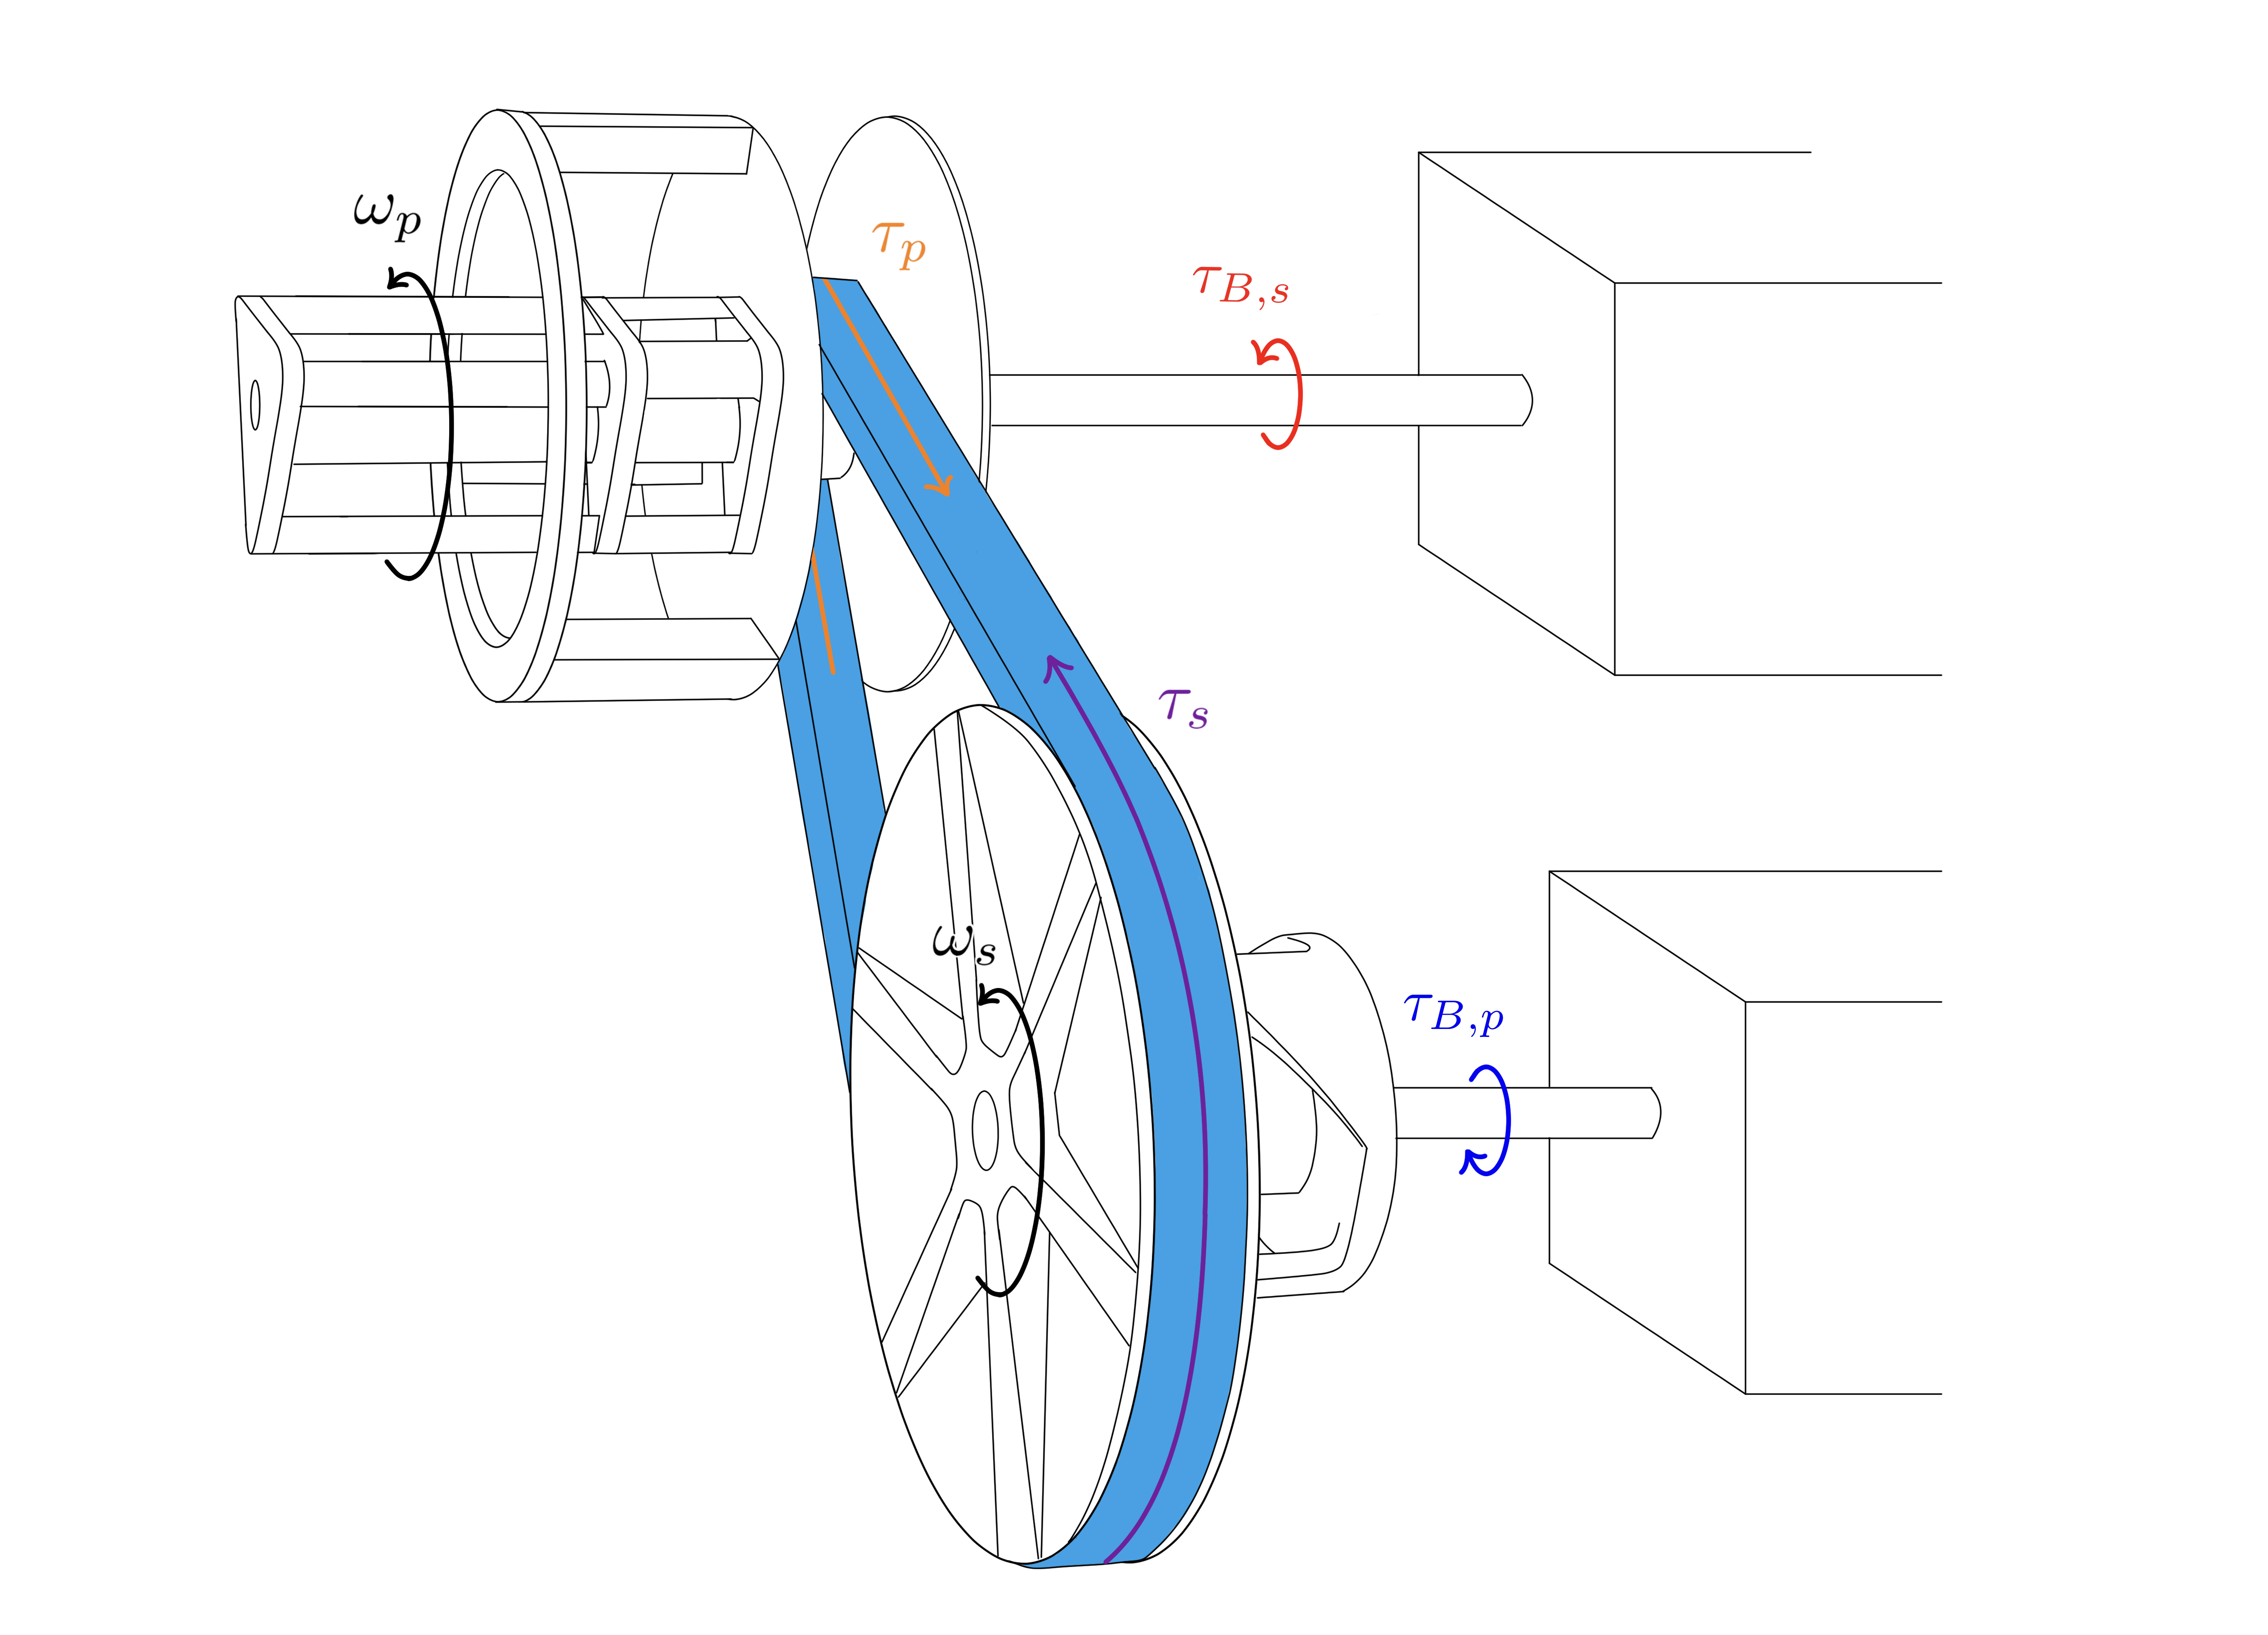
\includegraphics[width=\linewidth]
    {./figures/rotation/torque_path.png}
    \caption{
    Rotating systems and torque path of the engaged CVT. The shaft-side
    boundaries represent the torque and equivalent inertia presented by the
    attached systems. The belt remains outside the two pulley-side systems and
    interacts with them through the contact torques \(\tau_p\) and \(\tau_s\).
    The arrows show the signed directions associated with forward power
    transfer.
    }
    \label{fig:pulley_assembly_torque_path}
\end{figure}

Begin with the primary. When its speed changes, the primary shaft must
accelerate not only the pulley itself, but also the rotating hardware attached
beyond the CVT boundary. As established in
\Cref{sec:system_definition}, that external hardware is represented
at the shaft by the equivalent inertia \(I_{\mathrm{B},p}\), while
\(\tau_{\mathrm{B},p}\) is the torque it applies to the primary side. The
remaining external interaction is the belt, which exerts the torque \(\tau_p\)
on the primary pulley.

The secondary follows the same construction. Its attached hardware contributes
the equivalent inertia \(I_{\mathrm{B},s}\) and applies the boundary torque
\(\tau_{\mathrm{B},s}\), while the belt exerts \(\tau_s\) on the secondary
pulley.

The signs follow directly from the convention established in
\Cref{sec:rotational_sign}. During forward power transfer, the primary boundary
drives the primary pulley and the belt resists it. The belt then drives the
secondary pulley against the resisting secondary boundary. Thus,

\[
    \tau_{\mathrm{B},p}>0,
    \qquad
    \tau_p<0,
    \qquad
    \tau_s>0,
    \qquad
    \tau_{\mathrm{B},s}<0.
\]

Although the primary and secondary contain different mechanisms, their
rotational balances now have the same outer structure. Let \(j\in\{p,s\}\)
denote the pulley side under consideration.

The angular momentum on side \(j\) has two contributions. The fixed equivalent
boundary inertia rotates at \(\omega_j\), so it carries angular momentum
\(I_{\mathrm{B},j}\omega_j\). Let \(H_{\mathrm{CVT},j}\) denote the angular
momentum carried by the corresponding shaft and pulley assembly, including the
internal motions of its components. The total is therefore

\begin{equation}
    H_j
    =
    I_{\mathrm{B},j}\omega_j
    +
    H_{\mathrm{CVT},j}.
    \label{eq:pulley_side_total_angular_momentum}
\end{equation}

Bearing, seal, windage, and other unmodeled resisting torques are omitted
under \AssRef{assump:no_parasitic_losses}. Within the resulting pulley-side
free body, the applied boundary torque and belt torque are therefore the only
external torques retained. Newton's second law for rotation gives

\[
    \tau_{\mathrm{B},j}
    +
    \tau_j
    =
    \frac{dH_j}{dt}.
\]

Substituting \Cref{eq:pulley_side_total_angular_momentum} writes this as

\[
    \tau_{\mathrm{B},j}
    +
    \tau_j
    =
    \frac{d}{dt}
    \left(
        I_{\mathrm{B},j}\omega_j
        +
        H_{\mathrm{CVT},j}
    \right).
\]

The equivalent boundary inertia is fixed, so differentiating yields the common
pulley-side equation of motion:

\bigeq{eq:pulley_assembly_common_rotational_balance}
{Common Pulley-Side Rotational Balance}
{
\begin{aligned}
    \tau_{\mathrm{B},j}
    +
    \tau_j
    &=
    I_{\mathrm{B},j}\dot{\omega}_j
    +
    \frac{dH_{\mathrm{CVT},j}}{dt},
    \qquad
    j\in\{p,s\}.
\end{aligned}
}

The way shifting changes the angular momentum carried within a pulley is
contained in \(H_{\mathrm{CVT},j}\). On the primary, the flyweights
redistribute mass relative to the shaft as they pivot. On the secondary, the
movable sheave rotates relative to the shaft-side assembly as it follows the
helix. The two pulley sides therefore share the balance in
\Cref{eq:pulley_assembly_common_rotational_balance}, but require separate
expressions for their internal angular momentum. Beginning with the primary,
each assembly can now be examined in turn.


% --------------------------------------------------------------
\subsection{Primary Pulley Assembly}
\label{sec:primary_pulley_rotational_dynamics}

The primary is the simpler of the two pulley assemblies because nearly all of
its hardware shares the shaft speed \(\omega_p\). The shaft, sheaves, ramp
carrier, and other coaxial components may translate during a shift, but that
translation is along the shaft and therefore does not change their distance
from its axis. Their combined shaft-axis inertia can consequently be collected
into one constant quantity, \(I_{p,\mathrm{const}}\).

The flyweights are different. They are carried around the primary shaft at
\(\omega_p\), but their mass moves radially as they pivot. The same motion was
already used in \Cref{sec:primary_movable_sheave_balance} to determine the
centrifugal action that closes the primary. There, the flyweight geometry was
summarized by the shaft-axis inertia map \(J_{f,p}(x_p)\). Since
\(x_p=s\), that map is now \(J_{f,p}(s)\).

It is useful to recall what this inertia represents. The quantity
\(J_{f,p}\) measures the flyweight mass distribution about the \emph{primary
shaft}. It is therefore distinct from the constant pivot-axis inertia \(I_f\)
that appeared in the flyweight moment balance of
\Cref{eq:primary_flyweight_moment_balance}. The two quantities describe the
same flyweights about different axes and enter different equations of motion.

At a given shift position, the angular momentum carried inside the primary CVT
boundary is therefore

\begin{equation}
    H_{\mathrm{CVT},p}
    =
    \left[
        I_{p,\mathrm{const}}
        +
        J_{f,p}(s)
    \right]
    \omega_p.
    \label{eq:primary_pulley_angular_momentum}
\end{equation}

If the shift position were fixed, differentiating this expression would simply
multiply the current inertia by \(\dot\omega_p\). During a shift, however,
\(J_{f,p}\) changes as well. Because its only configuration variable is
\(s\), differentiating \Cref{eq:primary_pulley_angular_momentum} gives

\begin{equation}
    \frac{dH_{\mathrm{CVT},p}}{dt}
    =
    \left[
        I_{p,\mathrm{const}}
        +
        J_{f,p}(s)
    \right]
    \dot\omega_p
    +
    \frac{dJ_{f,p}}{ds}\dot s\,\omega_p.
    \label{eq:primary_pulley_angular_momentum_rate}
\end{equation}

The two terms describe different ways of changing the same angular momentum.
The first accelerates the primary with the flyweights held at their current
configuration. The second changes the angular momentum because the flyweight
mass itself moves toward or away from the shaft while already rotating.

Substituting this result into the common pulley-side balance from
\Cref{eq:pulley_assembly_common_rotational_balance} gives the primary equation
of motion:

\bigeq{eq:primary_rotational_eom_belt}
{Primary Pulley Rotational Balance}
{
\begin{aligned}
    \tau_{\mathrm{B},p}
    +
    \tau_p
    ={}&
    \left[
        I_{\mathrm{B},p}
        +
        I_{p,\mathrm{const}}
        +
        J_{f,p}(s)
    \right]
    \dot\omega_p
    \\
    &+
    \frac{dJ_{f,p}}{ds}\dot s\,\omega_p.
\end{aligned}
}

The connection to the axial flyweight balance is now explicit. In
\Cref{eq:primary_balance_in_shift_coordinate}, the derivative
\(dJ_{f,p}/ds\) determined how shaft rotation produces a centrifugal closing
action. Here, the same derivative determines how that closing motion changes
the shaft-axis angular momentum. The two appearances are not separate
flyweight corrections: they are the axial and rotational consequences of the
same radial redistribution of flyweight mass.

For the conventional primary mechanism, outward flyweight motion increases
\(J_{f,p}\). During an upshift, \(\dot s>0\), so the rotating primary must
supply the angular momentum required by that outward motion in addition to
accelerating the shaft. During a backshift the redistribution reverses, and
the flyweights return angular momentum to the shaft-side motion.

If the shift is held fixed, \(\dot s=0\), and the flyweight mass distribution
no longer changes. The additional term vanishes and the familiar fixed-inertia
form is recovered:

\begin{equation}
    \tau_{\mathrm{B},p}
    +
    \tau_p
    =
    \left[
        I_{\mathrm{B},p}
        +
        I_{p,\mathrm{const}}
        +
        J_{f,p}(s)
    \right]
    \dot\omega_p,
    \qquad
    \dot s=0.
    \label{eq:primary_rotational_fixed_configuration_limit}
\end{equation}

% --------------------------------------------------------------

\subsection{Secondary Pulley Assembly}
\label{sec:secondary_pulley_rotational_dynamics}

The secondary differs from the primary in one important way. During a shift,
the complete secondary remains one mechanical assembly, but not every part of
that assembly has the same angular speed.

The secondary shaft, fixed sheave, and hardware locked to them rotate at
\(\omega_s\). Let their combined shaft-axis inertia inside the CVT boundary be
\(I_{s,F}\). The movable sheave and the components rigidly attached to it have
inertia \(I_{s,M}\). As established while deriving the secondary axial balance,
the helix makes this movable assembly rotate relative to the shaft-side
assembly as it translates. Its absolute angular speed is therefore

\begin{equation}
    \omega_{s,M}
    =
    \omega_s
    +
    \frac{d\theta_s}{dx_s}\dot x_s,
    \label{eq:secondary_movable_sheave_speed_recalled}
\end{equation}

which is the relation already obtained in
\Cref{eq:secondary_movable_sheave_speed}. The angular momentum carried by the
secondary must therefore retain the two angular speeds separately:

\begin{equation}
    H_{\mathrm{CVT},s}
    =
    I_{s,F}\omega_s
    +
    I_{s,M}\omega_{s,M}.
    \label{eq:secondary_pulley_angular_momentum}
\end{equation}

The free body here is larger than the movable-sheave free body used in
\Cref{sec:secondary_rotational_loading}. There, only the movable assembly was
isolated, so the spring and helix torques crossed the boundary and had to
appear explicitly. Here, the shaft-side and movable-side hardware are enclosed
together. The torque exerted by the helix on the movable side is accompanied
by an equal-and-opposite torque on the shaft-side assembly, and both actions
lie inside the same free body. The torsional spring produces the same kind of
internal pair. These torques therefore cancel from the moment balance of the
complete secondary. Their mechanical effect has not disappeared: the helix
still allows the movable side to rotate at \(\omega_{s,M}\) rather than
\(\omega_s\), and that difference remains in
\Cref{eq:secondary_pulley_angular_momentum}.

The common pulley-side balance in
\Cref{eq:pulley_assembly_common_rotational_balance} requires the time rate of
change of the angular momentum inside this boundary. Because
\Cref{eq:secondary_pulley_angular_momentum} contains two angular velocities,
differentiating it requires the corresponding two angular accelerations:

\begin{equation}
    \frac{dH_{\mathrm{CVT},s}}{dt}
    =
    I_{s,F}\dot\omega_s
    +
    I_{s,M}\dot\omega_{s,M}.
    \label{eq:secondary_pulley_angular_momentum_rate_unmapped}
\end{equation}

The first acceleration, \(\dot\omega_s\), is the shaft acceleration governed
by the present rotational balance. The second is not another independent
degree of freedom. The helix already tied the movable-side rotation to the
axial sheave motion in \Cref{sec:secondary_movable_sheave_balance}. In
particular, differentiating the helix kinematics there gave
\Cref{eq:secondary_movable_sheave_acceleration}:

\begin{equation}
    \dot\omega_{s,M}
    =
    \dot\omega_s
    +
    \frac{d\theta_s}{dx_s}\ddot x_s
    +
    \frac{d^2\theta_s}{dx_s^2}\dot x_s^2.
    \label{eq:secondary_movable_sheave_acceleration_recalled}
\end{equation}

The rotational balance has therefore led back to a kinematic relation already
established by the axial mechanism. Substituting
\Cref{eq:secondary_movable_sheave_acceleration_recalled} into
\Cref{eq:secondary_pulley_angular_momentum_rate_unmapped} gives

\begin{equation}
\begin{aligned}
    \frac{dH_{\mathrm{CVT},s}}{dt}
    ={}&
    \left(I_{s,F}+I_{s,M}\right)\dot\omega_s
    \\
    &+
    I_{s,M}
    \left[
        \frac{d\theta_s}{dx_s}\ddot x_s
        +
        \frac{d^2\theta_s}{dx_s^2}\dot x_s^2
    \right].
\end{aligned}
    \label{eq:secondary_pulley_angular_momentum_rate}
\end{equation}

Substituting this rate into the common pulley-side rotational balance in
\Cref{eq:pulley_assembly_common_rotational_balance} produces the local
secondary equation of motion:

\bigeq{eq:secondary_rotational_eom_local}
{Secondary Pulley Rotational Balance}
{
\begin{aligned}
    \tau_{\mathrm{B},s}
    +
    \tau_s
    ={}&
    \left(
        I_{\mathrm{B},s}
        +
        I_{s,F}
        +
        I_{s,M}
    \right)
    \dot\omega_s
    \\
    &+
    I_{s,M}
    \left[
        \frac{d\theta_s}{dx_s}\ddot x_s
        +
        \frac{d^2\theta_s}{dx_s^2}\dot x_s^2
    \right].
\end{aligned}
}

The first term accelerates the rotation shared by the complete secondary. The
bracketed terms change only the movable side's rotation relative to the shaft.
They are the rotational counterpart of the helix-reflected inertia already
encountered in the secondary axial balance.

The complete CVT uses the shared shift coordinate rather than \(x_s\) as an
independent coordinate. The required mapping was already established in
\Cref{eq:secondary_local_to_shift_map}. Substituting

\[
    \dot x_s
    =
    \frac{dx_s}{ds}\dot s,
    \qquad
    \ddot x_s
    =
    \frac{dx_s}{ds}\ddot s
    +
    \frac{d^2x_s}{ds^2}\dot s^2
\]

into \Cref{eq:secondary_rotational_eom_local} gives the same rotational
balance in the coordinate used by the complete model:

\begin{equation}
\begin{aligned}
    \tau_{\mathrm{B},s}
    +
    \tau_s
    ={}&
    \left(
        I_{\mathrm{B},s}
        +
        I_{s,F}
        +
        I_{s,M}
    \right)
    \dot\omega_s
    \\
    &+
    I_{s,M}
    \frac{d\theta_s}{dx_s}
    \frac{dx_s}{ds}
    \ddot s
    \\
    &+
    I_{s,M}
    \left[
        \frac{d\theta_s}{dx_s}
        \frac{d^2x_s}{ds^2}
        +
        \frac{d^2\theta_s}{dx_s^2}
        \left(\frac{dx_s}{ds}\right)^2
    \right]
    \dot s^2.
\end{aligned}
    \label{eq:secondary_rotational_eom_belt}
\end{equation}

All local helix quantities in this expression are evaluated at
\(x_s=x_s(s)\). Its signs follow directly from the kinematics already chosen.
For the conventional helix,
\(d\theta_s/dx_s>0\), while the belt geometry gives \(dx_s/ds<0\) over the
engaged shift range. Hence

\[
    \frac{d\theta_s}{ds}
    =
    \frac{d\theta_s}{dx_s}
    \frac{dx_s}{ds}
    <0.
\]

During an upshift, \(\dot s>0\), so \(\dot\theta_s<0\): the secondary opens
and the movable side rotates more slowly than the shaft-side assembly. The
sign of the corresponding angular-momentum term is therefore carried by the
mechanism maps rather than assigned separately in the rotational balance.

If the shift is held fixed, \(\dot s=\ddot s=0\). The helix then produces no
relative motion, and the fixed and movable sides rotate together. The balance
reduces to

\begin{equation}
    \tau_{\mathrm{B},s}
    +
    \tau_s
    =
    \left(
        I_{\mathrm{B},s}
        +
        I_{s,F}
        +
        I_{s,M}
    \right)
    \dot\omega_s.
    \label{eq:secondary_rotational_fixed_configuration_limit}
\end{equation}

% --------------------------------------------------------------

\subsection{What the Rotational Balances Establish}
\label{sec:rotational_balance_synthesis}

The primary and secondary now have complete shaft-axis equations of motion.
Both remain direct statements of \(\sum\tau=dH/dt\). The additional terms
appear because the hardware that actuates the pulleys continues to move while
the pulley assemblies rotate, so shifting changes the angular momentum stored
inside the assemblies themselves.

On the primary, this connection is carried by the same flyweight inertia map
\(J_{f,p}(s)\) that appeared in the axial derivation. There,
\(dJ_{f,p}/ds\) contributes to the centrifugal closing action because the
flyweights move outward as the primary closes. Here, \(J_{f,p}(s)\) and its
derivative determine how much shaft-axis angular momentum those same
flyweights carry as their radial mass distribution changes. The axial and
rotational balances are therefore two views of the same flyweight motion: one
asks how rotation drives the movable sheave, while the other asks how that
moving flyweight mass changes the rotational response of the pulley.

The secondary shows the same reciprocity through \(I_{s,M}\) and the helix map
\(\theta_s(x_s)\). In the axial balance, the helix reflects the movable
assembly's rotational inertia into the sheave motion, so part of the available
torque is required to change the movable side's rotation before the remainder
appears as axial force. In the rotational balance, that same relative motion
means the movable side carries angular momentum at a speed different from the
shaft-side assembly, so the axial shift acceleration enters the shaft-axis
balance. Again, the two equations are describing one constrained piece of
hardware from different free bodies.

Mechanical actuation therefore creates a direct coupling between the axial and
rotational dynamics inside each pulley assembly. This is distinct from the
coupling carried by the belt reaction. Belt contact can connect the two kinds
of balance because its normal action loads the sheaves axially while its
tangential action transmits torque about the shafts. The present terms add a
second path: the flyweight and helix mechanisms that generate the clamping
response also carry inertia, so their own motion appears directly in the
rotational equations. The actuator is therefore part of both balances, rather
than acting only as a source of clamping force whose influence reaches shaft
rotation through the belt.

This distinction gives a precise comparison with earlier transient models.
In the rubber-belt formulation of \citet{Ballew2015}, belt-contact torque
changes pulley speed through a fixed lumped pulley inertia, while pulley axial
force is supplied to the belt model. Axial and rotational behaviour can still
interact through the belt solution, but motion of the clamping hardware does
not alter the pulley angular momentum itself. \citet{DuanEtAl2016} provide a
stronger adjacent precedent in a chain CVT: rotational dynamics, movable-pulley
axial dynamics, chain motion, and contact forces are solved as a coupled
system. Their shaft balance nevertheless retains a fixed pulley inertia, while
the movable-pulley mass appears in a separate axial equation. The coupling is
therefore carried through the chain, contact forces, and changing radius rather
than through actuator motion entering both balances.

A mechanically actuated rubber-belt comparison is provided by
\citet{SilvaEtAl2023}, who retain axial equations for both movable sheaves and
reduce their translations to a shared shift coordinate. Their rotational
treatment uses a fixed primary-pulley inertia. This establishes direct
precedent for mechanical clamping, movable-sheave inertia, and coupled shift
motion, but not for the additional shaft-axis angular-momentum terms produced
by the moving actuator hardware.

The helical model of \citet{SorgeCammalleri2011} provides a complementary
secondary comparison. Their formulation resolves the relative motion of the
driven sheaves and the generally unequal belt torques acting on the two faces
in substantially greater local detail. That work therefore captures secondary
helix and face-contact mechanics that are reduced here. The distinction in the
present balance is different: the helix-constrained movable assembly is
retained as part of the complete secondary angular momentum, so the same
relative motion that appears in its axial dynamics also appears in the
shaft-axis equation.

Taken together, these comparisons show that axial--rotational coupling itself
is not the new ingredient. Existing formulations can produce that coupling
through belt or chain reactions, changing radii, and shared shift motion. Among
the reviewed reduced-order formulations for mechanically actuated rubber-belt
CVTs, however, no equivalent pair of pulley balances was identified in which
the moving clamping hardware itself provides this additional inertial coupling
on both sides: the primary flyweights change their shaft-axis mass distribution
as they generate closing action, while the secondary movable assembly changes
its shaft-axis angular momentum through the same helix motion that produces
its axial response.

The result is a single mechanical picture of each pulley rather than separate
axial and rotational descriptions joined only through transmitted load. The
same mechanism maps that determine how the pulley clamps also determine how
its internal motion changes the shaft dynamics. When those actuator motions
cease, the additional terms vanish and the familiar fixed-configuration
inertia balances are recovered.

\section{Belt Transport and Pulley Contact Mechanics}
\label{sec:belt_transport_contact}

The preceding sections established the axial and rotational equations of
motion for the two pulley assemblies, but both stop at the same remaining
mechanical body: the belt. The axial balances still contain the belt normal
loads \(N_p\) and \(N_s\), while the rotational balances contain the belt
torques \(\tau_p\) and \(\tau_s\). The belt transport speed \(v_b\) is also
retained as a state, but its acceleration has not yet been established.

So far, each of these quantities has appeared only through the action of the
belt on one of the pulley assemblies. Newton's third law gives the same
interactions from the opposite side. The force and torque exerted by the belt
on a pulley are accompanied by equal-and-opposite actions on the belt itself.
The remaining mechanics can therefore be viewed from the belt rather than
from either pulley.

This change of free body is important because the belt is not two independent
contacts. It is one closed body connecting both pulley assemblies. Whatever
forces and torques are exchanged at the primary must coexist with those at the
secondary and with the motion of the belt between them. The belt mechanics
must therefore be self-consistent around the complete loop.

\subsection{Complete-Belt Transport}

\label{sec:complete_belt_transport}

The belt transport speed provides the natural starting point. The belt speed
\(v_b\) can change only if something pushes or pulls the belt along its path.
Those tangential actions come from the primary and secondary pulley contacts.
The belt's transport acceleration must therefore come from the two pulley
wraps.

At either wrap, the mechanism is simple. The pulley contact has both normal
and tangential components. Normal contact acts perpendicular to the local belt
path, so it cannot push or pull the belt in the direction that defines \(v_b\).
Frictional traction, by contrast, is spread over the contact and acts tangent
to the belt at every point. Traction acting in the direction of belt travel
does positive work on the belt, while traction acting against belt travel does
negative work and removes energy from it. Moreover, when the complete closed
belt is considered, the tensions between adjacent belt sections are internal
and cancel. The primary and secondary tractions are therefore the only external
actions that can change the belt's transport speed.

Each small traction force also acts at a radius from the shaft and therefore
produces a small moment on the pulley. Adding these moments around the wrap
gives the contact torque \(\tau_j\) already used in the pulley rotational
balance. Thus, \(\tau_j\) is simply the accumulated turning effect of the same
tangential contact forces that can change \(v_b\).

Newton's third law places equal-and-opposite traction forces on the belt. Their
total moment is therefore \(-\tau_j\), and at the effective contact radius
\(r_{j,\mathrm{eff}}\), they are equivalent to the net tangential pull
\(-\tau_j/r_{j,\mathrm{eff}}\). If the pull at one wrap supplies exactly the
power removed by the pull at the other, the belt simply carries that power
between the pulleys. If the two actions do not balance, the resulting energy
excess or deficit must be taken up by the belt.

The belt assumptions leave that imbalance only one place to go. The fixed
length of \AssRef{assump:constant_belt_length} excludes longitudinal extension
and the strain energy it would store. The single transport coordinate of
\AssRef{assump:single_belt_speed} gives every belt region the same speed
\(v_b\), so one region cannot speed up independently of the rest. The belt's
only retained longitudinal energy is therefore
\(\tfrac{1}{2}m_bv_b^2\). Net power into the belt increases \(v_b\); net power
out decreases it.

The energy argument now explains why an imbalance between the pulley actions
must change \(v_b\). Newton's second law determines the corresponding signed
acceleration directly, where the whole belt loop is treated as a single body.
Place one boundary around the entire loop. From the force accounting above, the
only external tangential actions on this free body are the two equivalent
pulley pulls, acting on the complete belt mass \(m_b\). The complete-belt
transport balance is therefore

\bigeq{eq:complete_belt_transport_newton}
{Complete-Belt Transport Balance}
{
  \begin{aligned}
    \sum F_{b,t}^{\mathrm{ext}}
    &=
    -\frac{\tau_p}{r_{p,\mathrm{eff}}}
    -\frac{\tau_s}{r_{s,\mathrm{eff}}}
    \\
    &=
    \frac{d}{dt}\left(m_bv_b\right)
    =
    m_b\dot v_b.
  \end{aligned}
}

This balance gives the basic longitudinal motion of the belt. If the two
pulley contacts exert a net force in the positive belt direction, the belt
speeds up; if they exert a net force in the opposite direction, it slows down.
If the two actions balance, the belt can carry power between the pulleys
without changing \(v_b\).

\medskip

\noindent{\large\bfseries Interpreting the Transport Balance}

\par\smallskip

As far as speeding up or slowing down the complete belt is concerned, this
result is sufficient. The quantity \(v_b\), however, describes only how quickly
belt material travels along its prescribed path. Consider one marked piece of
belt. It approaches a pulley along one straight span and leaves along the
other. Its direction of travel has changed. The complete-belt balance says how
its speed changes, but contains nothing that explains this change in direction.
Left to itself, the marked piece would continue straight past the pulley. Its
motion around the wrap is therefore possible only because forces act on it
throughout that turn.

The clearest way to separate these forces from the transport motion is to
remove the motion altogether. Consider first the familiar case of a rope
wrapped around a classical pulley. Pull equally on the two ends of the rope.
If both pulls are increased together, the tension throughout the rope rises
and the pulley becomes more heavily loaded, even though no tension difference
has been introduced. The taut rope is redirected around the pulley, and in
doing so it exerts a resultant load on it. The pulley supplies the
corresponding equal-and-opposite contact reaction.

The same basic effect occurs when the CVT belt is wrapped around a sheave.
Suppose the belt and pulley are stationary and the entry and exit tensions are
both \(500\,\mathrm{N}\). Their difference is zero, so there is no transmitted
torque or longitudinal acceleration, yet the tensioned belt still loads the
pulley through the wrap. Raising both the entry and exit tensions to
\(1000\,\mathrm{N}\) changes neither the tension difference nor the belt's
motion, but the belt now loads the pulley more strongly and the corresponding
normal contact increases. The geometry and motion have not changed; the pulley
loading has.

The loading described above is carried through the belt--sheave contact around
the wrap. In the model, the resultant normal contact loads on the primary and
secondary pulleys are denoted by \(N_p\) and \(N_s\). Their axial components
already appear in the primary and secondary movable-sheave balances; see
\Cref{eq:completed_primary_axial_balance,eq:completed_secondary_axial_balance}.
The static example therefore has an important consequence: even with no
transmitted torque or belt acceleration, changing the belt tension changes
\(N_p\) and \(N_s\), and can therefore change the shift balance. Determining
these normal loads requires knowing the tension carried around each pulley.
The remaining difficulty is that this tension is not generally constant around
the pulley.

As established above, a pulley transfers torque through tangential traction
distributed around its wrap. As the belt passes through the contact, this
traction changes how strongly the belt is being pulled. The tension leaving
the wrap therefore generally differs from the tension entering it. In the
simplest steady, inertia-free picture, the transmitted torque is equal to the
pulley radius multiplied by this tension difference. Retaining the inertia of
the wrapped belt modifies that balance, but not the basic interpretation:
torque transfer tells us how the tension changes through the contact.

The quantity needed to determine the normal loading is therefore itself
changing as the belt moves through the wrap. Knowing the entry and exit
tensions tells us only how that process begins and ends, not what tension is
carried at each point between them. The normal contact must therefore be
determined locally as well.

\subsection{Local Equations of Motion on a Pulley Wrap}
\label{sec:local_wrap_dynamics}

The previous subsection leaves one local question: how is the tension carried
at a particular point in the wrap related to the contact force acting there?
The next step is therefore to build the free-body diagram of an infinitesimal
piece of belt within the wrap of either pulley \(j\in\{p,s\}\).

Let \(\theta\) increase through the wrap in the positive belt-transport
direction defined in \Cref{sec:rotational_sign}, and isolate the piece bounded
by cuts at \(\theta\) and \(\theta+d\theta\). Let \(T_j(\theta)\) denote the
tension carried by the belt at angular position \(\theta\). The tensions at
the two cuts are therefore \(T_j(\theta)\) and
\(T_j(\theta+d\theta)\). To keep the labels in the free-body diagram compact,
define

\begin{equation}
    T_j
    \equiv
    T_j(\theta),
    \qquad
    dT_j
    \equiv
    T_j(\theta+d\theta)-T_j(\theta).
    \label{eq:wrap_tension_increment_definition}
\end{equation}

The tension at the second cut can then be written exactly as \(T_j+dT_j\).
Thus, \(dT_j\) is the signed change in tension across the element: it is
positive if the tension increases with \(\theta\) and negative if the tension
decreases. No direction of change has yet been assumed.

Once the piece is cut free, the surrounding belt pulls on its two exposed
ends. Under \AssRef{assump:prescribed_belt_path}, the belt is perfectly
flexible and follows the prescribed planar path. Each cut therefore carries
only a longitudinal tension force directed along the local belt tangent; there
is no transverse shear force or bending moment. At both cuts, the surrounding
belt pulls away from the isolated piece.

Because the belt curves around the pulley, those two tension forces do not
point in the same direction. The belt tangent turns through \(d\theta\) from
one cut to the other. It is therefore convenient to draw the local directions
at the midpoint of the element. Using the radial and tangential convention
introduced in \Cref{sec:radial_direction}, \(\hat{\mathbf e}_r\) points
radially outward from the pulley axis, while \(\hat{\mathbf e}_\theta\) points
with increasing \(\theta\). Each end tangent is inclined by \(d\theta/2\) from
the midpoint tangent. The left-hand view in
\Cref{fig:infinitesimal_belt_element} shows this in-plane geometry.

The pulley also acts on the element through both sheave faces. To complete the
free-body diagram, these contact forces must be added to the cut-end tensions.
Their geometry cannot be represented clearly in the pulley plane, so the
right-hand view in \Cref{fig:infinitesimal_belt_element} shows the cross-section
of the same element. Under \AssRef{assump:fixed-belt-cross-section}, its shape
and mass centroid remain fixed. Under
\AssRef{assump:symmetric_face_sharing}, the two faces carry equal shares of the
normal contact. Let \(dN_j\) denote the sum of the magnitudes of the two
face-normal forces; each face therefore exerts a force of magnitude
\(dN_j/2\). Their axial components oppose one another and cancel, whereas their
outward radial components add to \(dN_j\sin\beta\).

The remaining contact action is tangential. Under
\AssRef{assump:gross_coulomb_traction}, let \(dF_{t,j}\) denote the resultant
tangential force exerted by both sheave faces on the element. It is defined as
positive when it acts in the direction of increasing \(\theta\); its actual
sign will be determined by the contact state. Because this force acts in the
pulley plane, it appears in the left-hand view of
\Cref{fig:infinitesimal_belt_element}. The two views therefore complete a
single free-body diagram: the left shows the forces acting around the wrap,
while the right shows how the two face-normal forces produce the radial
contact force appearing on the left.

\begin{figure}[H]
    \centering
    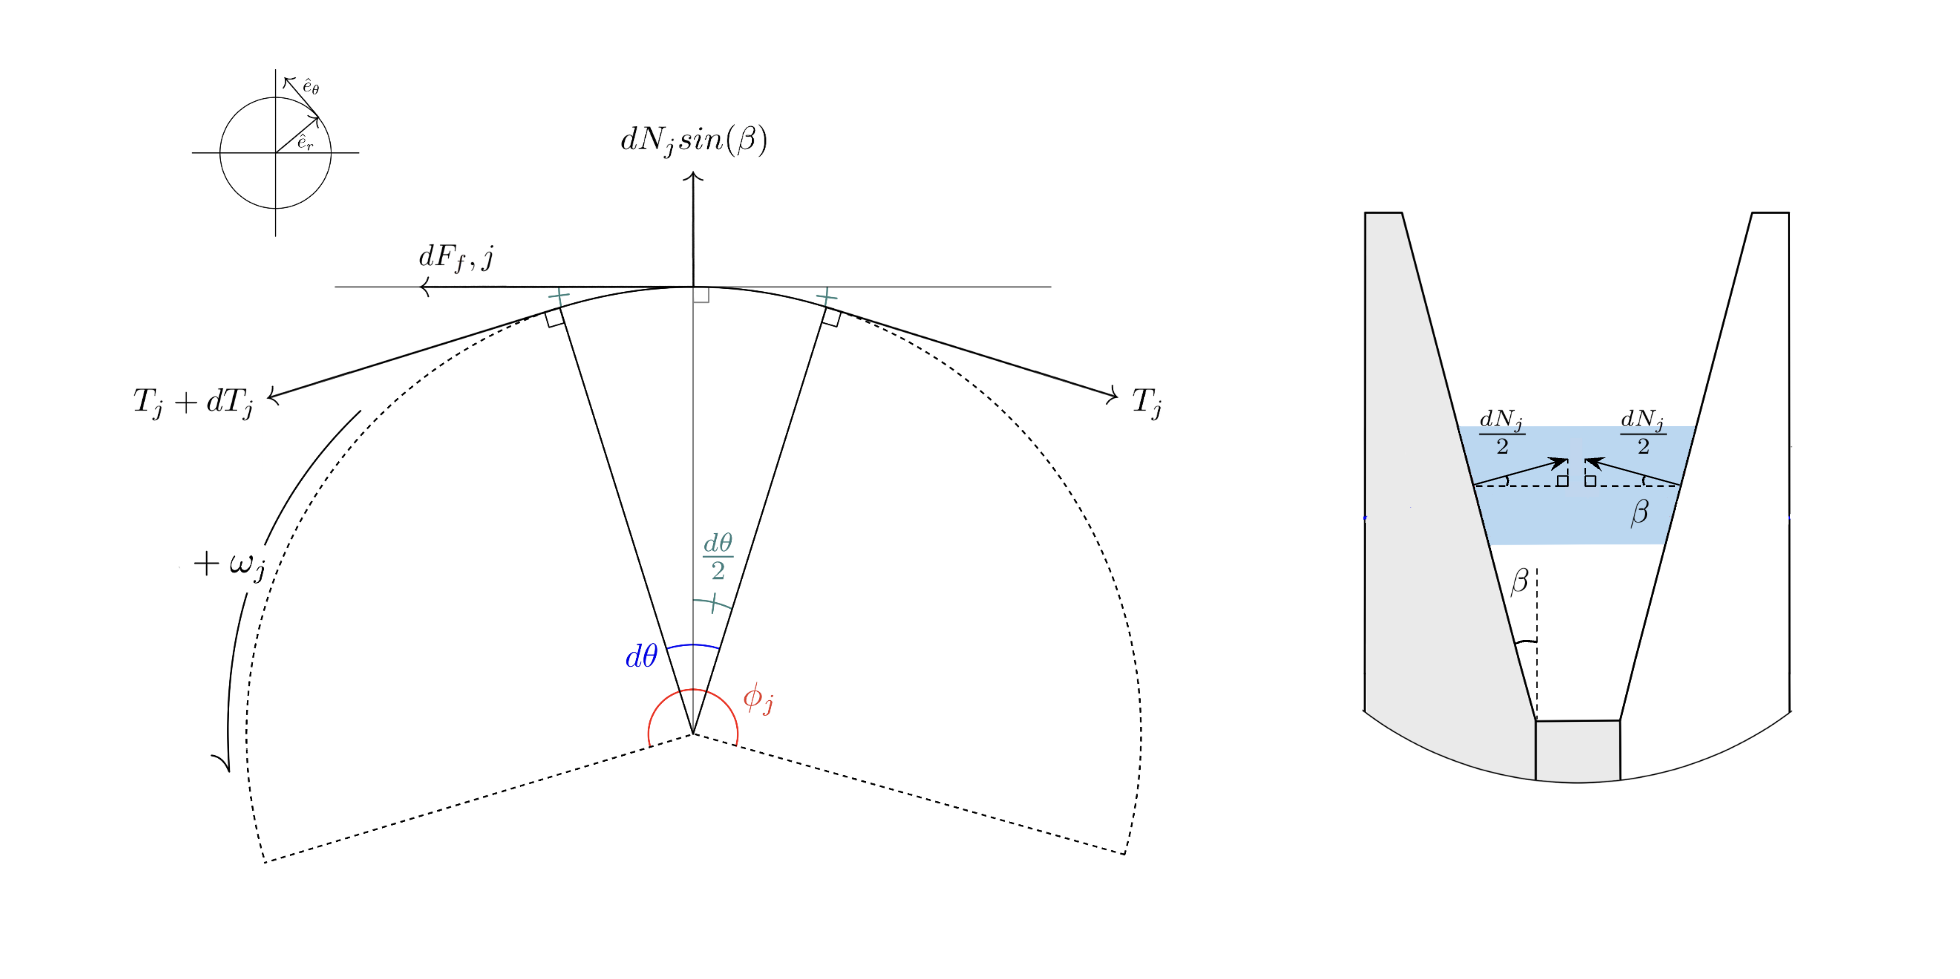
\includegraphics[width=\linewidth]
    {./figures/belt/infinitesimal_belt_element.png}
    \caption{Two views of the same infinitesimal belt element, bounded by
    \(\theta\) and \(\theta+d\theta\) within the wrap of pulley \(j\).
    The in-plane free-body diagram on the left shows the cut-end tensions
    \(T_j=T_j(\theta)\) and
    \(T_j+dT_j=T_j(\theta+d\theta)\), the midpoint directions, the
    half-angle \(d\theta/2\), the signed tangential contact force
    \(dF_{t,j}\), and the outward radial contact force
    \(dN_j\sin\beta\). The cross-section on the right shows the two
    face-normal forces of magnitude \(dN_j/2\), whose axial components
    cancel and whose radial components add.}
    \label{fig:infinitesimal_belt_element}
\end{figure}

\paragraph{Equations of motion for the infinitesimal element}

With the free-body diagram complete, Newton's second law can now be assembled
in the two local directions. The radial direction comes first because it
contains the normal contact that motivated the local analysis.

In the radial direction, the two sheave-face forces supply the combined
outward component \(dN_j\sin\beta\). The surrounding belt pulls inward at
both cuts. Since each end tangent is inclined by \(d\theta/2\) from the
midpoint tangent, the corresponding inward components are
\(T_j\sin(d\theta/2)\) and
\((T_j+dT_j)\sin(d\theta/2)\). Taking outward as positive, Newton's second law
therefore gives

\begin{equation}
    dN_j\sin\beta
    -
    T_j\sin\!\left(\frac{d\theta}{2}\right)
    -
    \left(T_j+dT_j\right)
    \sin\!\left(\frac{d\theta}{2}\right)
    =
    dm_j a_{r,j},
    \label{eq:wrap_radial_balance_start}
\end{equation}

where \(dm_j\) is the mass of the element and \(a_{r,j}\) is its signed
acceleration in the outward radial direction.

The same element must also satisfy Newton's second law in the tangential
direction. The face-normal forces have no tangential component. At the cut at
\(\theta\), the tension pulls opposite increasing \(\theta\), giving the
component \(-T_j\cos(d\theta/2)\). At the cut at
\(\theta+d\theta\), the tension pulls with increasing \(\theta\), giving
\((T_j+dT_j)\cos(d\theta/2)\). Including the signed tangential contact force
\(dF_{t,j}\), the tangential equation is therefore

\begin{equation}
    \left(T_j+dT_j\right)
    \cos\!\left(\frac{d\theta}{2}\right)
    -
    T_j\cos\!\left(\frac{d\theta}{2}\right)
    +
    dF_{t,j}
    =
    dm_j a_{\theta,j},
    \label{eq:wrap_tangential_balance_start}
\end{equation}

where \(a_{\theta,j}\) is the signed acceleration in the direction of
increasing \(\theta\).

The force side of each equation is now fully determined by the free-body
diagram. Their right-hand sides still express the belt element's response only
in the general form of mass times acceleration. Reducing them requires knowing
how much belt mass lies within the angle \(d\theta\), and how that material
accelerates while it travels around a pulley whose wrap radius can
simultaneously move as the CVT shifts. These quantities follow from the belt
cross-section and the radius kinematics already established in
\Cref{sec:geometry}.

\paragraph{Mass and motion of the belt element}

The mass and acceleration of the element must be evaluated at the belt's mass
centroid. As established in
\Cref{eq:geometry_radius_convention,eq:local_belt_mass_centroid_radius},
\(r_j\) locates the outer surface used to describe where the belt is seated,
whereas \(r_{j,\mathrm{cm}}\) locates the mass centroid. Under
\AssRef{assump:fixed-belt-cross-section}, the centroid remains a fixed radial
distance from the outer surface. Its radial velocity and acceleration are
therefore the radius rate and acceleration already derived for the seated
belt:

\[
    \dot r_{j,\mathrm{cm}}
    =
    \dot r_j,
    \qquad
    \ddot r_{j,\mathrm{cm}}
    =
    \ddot r_j.
\]

The element spans the angle \(d\theta\), so its arc length at the mass
centroid is \(r_{j,\mathrm{cm}}d\theta\). Multiplying this length by the belt
cross-sectional area \(A_b\) from
\Cref{eq:local_belt_cross_section_area} and the belt density \(\rho_b\) gives
the element mass:

\begin{equation}
    dm_j
    =
    \rho_b A_b r_{j,\mathrm{cm}}\,d\theta.
    \label{eq:wrap_element_mass}
\end{equation}

The element can move in two directions at once. It moves radially with the
shifting wrap at speed \(\dot r_j\), while the belt's transport carries it
tangentially at speed \(v_b\). Its velocity is therefore

\begin{equation}
    \mathbf v_{b,j}
    =
    \dot r_j\,\hat{\mathbf e}_r
    +
    v_b\,\hat{\mathbf e}_\theta.
    \label{eq:wrap_element_velocity}
\end{equation}

Acceleration is the time derivative of this velocity. Both scalar speeds can
change, but the local directions also change as the element travels around the
pulley. Differentiating while retaining both effects gives

\begin{align}
    \mathbf a_{b,j}
    &=
    \frac{d}{dt}
    \left(
        \dot r_j\hat{\mathbf e}_r
        +
        v_b\hat{\mathbf e}_\theta
    \right)
    \notag\\
    &=
    \ddot r_j\hat{\mathbf e}_r
    +
    \dot r_j\dot{\hat{\mathbf e}}_r
    +
    \dot v_b\hat{\mathbf e}_\theta
    +
    v_b\dot{\hat{\mathbf e}}_\theta.
    \label{eq:wrap_element_acceleration_unresolved}
\end{align}

The two basis-vector derivatives follow from how quickly the element moves
around the wrap. At the centroidal radius, its tangential speed and angular
rate are related by

\begin{equation}
    v_b
    =
    r_{j,\mathrm{cm}}\dot\theta,
    \qquad
    \dot\theta
    =
    \frac{v_b}{r_{j,\mathrm{cm}}}.
    \label{eq:wrap_element_angular_rate}
\end{equation}

As \(\theta\) increases, the outward radial direction turns toward
\(\hat{\mathbf e}_\theta\), while the tangential direction turns toward
\(-\hat{\mathbf e}_r\). Multiplying these changes per unit angle by the
angular rate in \Cref{eq:wrap_element_angular_rate} gives

\begin{equation}
    \dot{\hat{\mathbf e}}_r
    =
    \frac{v_b}{r_{j,\mathrm{cm}}}\hat{\mathbf e}_\theta,
    \qquad
    \dot{\hat{\mathbf e}}_\theta
    =
    -\frac{v_b}{r_{j,\mathrm{cm}}}\hat{\mathbf e}_r.
    \label{eq:wrap_element_basis_rates}
\end{equation}

Substituting these basis rates into
\Cref{eq:wrap_element_acceleration_unresolved} and collecting the radial and
tangential terms gives

\begin{align}
    \mathbf a_{b,j}
    &=
    \left(
        \ddot r_j
        -
        \frac{v_b^2}{r_{j,\mathrm{cm}}}
    \right)
    \hat{\mathbf e}_r
    +
    \left(
        \dot v_b
        +
        \frac{\dot r_jv_b}{r_{j,\mathrm{cm}}}
    \right)
    \hat{\mathbf e}_\theta.
    \label{eq:wrap_element_acceleration_expansion}
\end{align}

The acceleration components required by the two equations of motion are
therefore

\begin{align}
    a_{r,j}
    &=
    \ddot r_j
    -
    \frac{v_b^2}{r_{j,\mathrm{cm}}},
    \label{eq:wrap_radial_acceleration}
    \\
    a_{\theta,j}
    &=
    \dot v_b
    +
    \frac{\dot r_jv_b}{r_{j,\mathrm{cm}}}.
    \label{eq:wrap_tangential_acceleration}
\end{align}

The radial component contains the outward acceleration of the shifting wrap
and the familiar inward centripetal acceleration produced as the belt turns
around the pulley. The tangential component contains the change in belt speed
and an additional contribution from the radial velocity changing direction as
the element moves through the wrap. Together with
\Cref{eq:wrap_element_mass}, these two components now provide the complete
inertial sides of the radial and tangential balances.

\paragraph{Radial equation of motion}

We first return to the radial balance in
\Cref{eq:wrap_radial_balance_start}. Substituting the element mass from
\Cref{eq:wrap_element_mass} and the radial acceleration from
\Cref{eq:wrap_radial_acceleration}, then collecting the two inward tension
components, gives

\begin{equation}
    dN_j\sin\beta
    -
    \left(2T_j+dT_j\right)
    \sin\!\left(\frac{d\theta}{2}\right)
    =
    \rho_bA_b
    \left(
        r_{j,\mathrm{cm}}\ddot r_j-v_b^2
    \right)d\theta.
    \label{eq:wrap_radial_balance_expanded}
\end{equation}

The desired local quantity is the normal contact carried per unit wrap angle,
\(dN_j/d\theta\). Dividing
\Cref{eq:wrap_radial_balance_expanded} by \(d\theta\) gives

\[
    \sin\beta\,\frac{dN_j}{d\theta}
    -
    \left(2T_j+dT_j\right)
    \frac{\sin(d\theta/2)}{d\theta}
    =
    \rho_bA_b
    \left(
        r_{j,\mathrm{cm}}\ddot r_j-v_b^2
    \right).
\]

Only the tension term still depends on the finite angular width of the
element. To put its sine factor into the standard small-angle form, write

\[
    \frac{\sin(d\theta/2)}{d\theta}
    =
    \frac{1}{2}
    \frac{\sin(d\theta/2)}{d\theta/2}.
\]

Redistributing this factor of \(1/2\) through \(2T_j+dT_j\), the radial
balance can be written directly as

\[
    \sin\beta\,\frac{dN_j}{d\theta}
    -
    \left(T_j+\frac{dT_j}{2}\right)
    \frac{\sin(d\theta/2)}{d\theta/2}
    =
    \rho_bA_b
    \left(
        r_{j,\mathrm{cm}}\ddot r_j-v_b^2
    \right).
\]

The infinitesimal element is obtained by taking
\(d\theta\rightarrow0\). Because
\(dT_j=T_j(\theta+d\theta)-T_j(\theta)\), continuity of the tension field
gives \(dT_j\rightarrow0\). At the same time, the small-angle ratio tends to
one:

\[
    T_j+\frac{dT_j}{2}
    \longrightarrow
    T_j,
    \qquad
    \frac{\sin(d\theta/2)}{d\theta/2}
    \longrightarrow
    1.
\]

The complete local radial balance is consequently

\begin{equation}
\boxed{
    \sin\beta\,
    \frac{dN_j}{d\theta}
    =
    T_j
    -
    \rho_bA_b
    \left(
        v_b^2-r_{j,\mathrm{cm}}\ddot r_j
    \right).
}
    \label{eq:wrap_radial_balance}
\end{equation}

To see the physical meaning of this result most clearly, it is useful first to
consider a stationary belt on a fixed wrap. Setting \(v_b=0\) and
\(\ddot r_j=0\) gives

\begin{equation}
    \sin\beta\,
    \frac{dN_j}{d\theta}
    =
    T_j.
    \label{eq:wrap_static_radial_balance}
\end{equation}

We now recover the result anticipated from the physical picture: increasing
the belt tension increases the normal loading carried per unit wrap angle.
This remains true even when the tension is uniform through the contact, so
there is no tension difference and no torque is transmitted. The normal
loading therefore depends on the absolute tension level, not only on the
tension difference across the wrap.

Returning to the full balance, motion modifies this stationary relationship.
As the belt turns around the pulley, part of the inward tension is required to
provide its centripetal acceleration, reducing the outward sheave reaction at
a given tension. An outward wrap acceleration has the opposite effect and
increases that reaction.

\paragraph{Tangential equation of motion}

Finally, we complete the tangential equation of motion introduced in
\Cref{eq:wrap_tangential_balance_start}. Substituting the element mass from
\Cref{eq:wrap_element_mass} and the tangential acceleration from
\Cref{eq:wrap_tangential_acceleration} gives the complete balance

\begin{equation}
    \left(T_j+dT_j\right)
    \cos\!\left(\frac{d\theta}{2}\right)
    -
    T_j\cos\!\left(\frac{d\theta}{2}\right)
    +
    dF_{t,j}
    =
    \rho_bA_b r_{j,\mathrm{cm}}d\theta
    \left(
        \dot v_b
        +
        \frac{\dot r_jv_b}{r_{j,\mathrm{cm}}}
    \right).
    \label{eq:wrap_tangential_balance_with_motion}
\end{equation}

The desired result is again a local relation per unit wrap angle. Cancelling
the common \(T_j\) contribution from the two end tensions, simplifying the
acceleration term, and dividing through by \(d\theta\) gives

\[
    \frac{dT_j}{d\theta}
    \cos\!\left(\frac{d\theta}{2}\right)
    +
    \frac{dF_{t,j}}{d\theta}
    =
    \rho_bA_b
    \left(
        r_{j,\mathrm{cm}}\dot v_b
        +
        \dot r_jv_b
    \right).
\]

The remaining cosine records that the end tensions are not quite parallel on
a finite element. In the infinitesimal limit, the two end tangents coincide
and

\[
    \lim_{d\theta\rightarrow0}
    \cos\!\left(\frac{d\theta}{2}\right)
    =
    \cos(0)
    =
    1.
\]

The cosine therefore becomes a factor of one; the tension-gradient term
remains. The local tangential equation of motion is

\begin{equation}
    \frac{dT_j}{d\theta}
    +
    \frac{dF_{t,j}}{d\theta}
    =
    \rho_bA_b
    \left(
        r_{j,\mathrm{cm}}\dot v_b
        +
        \dot r_jv_b
    \right).
    \label{eq:wrap_tangential_balance_force}
\end{equation}

This balance identifies the two tangential forces acting per unit wrap angle:
the change in belt tension and the traction supplied by the pulley. Their sum
produces the tangential acceleration of the belt. What remains is to relate
that tangential contact force to the normal contact already present in the
radial balance.

Under \AssRef{assump:gross_coulomb_traction}, the sheave contact obeys Coulomb
friction. While the belt sticks, the tangential force is a reaction that can
act in either direction and take any magnitude up to the static limit. Once
the belt slides, its magnitude is fixed by kinetic friction and its direction
opposes the relative sliding. Both cases relate the tangential force on the
element to the same normal-force increment \(dN_j\), but with different rules
for the allowable proportionality.

Rather than carrying a separate magnitude condition and direction sign
through the remaining equations, define the signed traction utilization
\(\lambda_j\) by

\bigeq{eq:lambda_local_definition}
{Signed Traction Utilization}
{
    dF_{t,j}
    =
    \lambda_j\,dN_j,
    \qquad
    \lambda_j
    =
    \begin{cases}
        \lambda_{j,\mathrm{st}},
        \quad
        \left|\lambda_{j,\mathrm{st}}\right|\leq\mu_s,
        & \text{sticking},
        \\
        \sigma_j\mu_k,
        \quad
        \sigma_j\in\{-1,+1\},
        & \text{sliding}.
    \end{cases}
}

The magnitude of \(\lambda_j\) gives the tangential force used per unit normal
load, while its sign gives the direction of that force. Thus,
\(\lambda_j>0\) acts with increasing \(\theta\),
\(\lambda_j<0\) acts against it, and \(\lambda_j=0\) represents normal contact
with no tangential force. In sliding, \(\sigma_j\) selects the direction that
opposes the relative motion, while \(\mu_k\) fixes the magnitude. Under
\AssRef{assump:wrap_contact_resolution}, one value of \(\lambda_j\) represents
the complete wrap at a given instant.

Dividing \(dF_{t,j}=\lambda_jdN_j\) by \(d\theta\) and substituting it into
\Cref{eq:wrap_tangential_balance_force} gives the complete local tangential
balance:

\begin{equation}
\boxed{
    \frac{dT_j}{d\theta}
    +
    \lambda_j\frac{dN_j}{d\theta}
    =
    \rho_bA_b
    \left(
        r_{j,\mathrm{cm}}\dot v_b
        +
        \dot r_jv_b
    \right).
}
    \label{eq:wrap_tangential_balance}
\end{equation}

To expose the physical meaning of this result, it is useful again to remove
the effects of motion. For a fixed wrap and steady belt speed,
\(\dot r_j=0\) and \(\dot v_b=0\), so the tangential inertia vanishes and the
balance becomes

\begin{equation}
    \frac{dT_j}{d\theta}
    =
    -\lambda_j\frac{dN_j}{d\theta}.
    \label{eq:wrap_steady_tangential_balance}
\end{equation}

We now recover the expected local relationship:
the pulley traction must be balanced by an equal and opposite tension
gradient. Traction therefore forces the tension to evolve around the wrap, and
integrating this local evolution produces the tension difference associated
with transmitted torque. Since the normal contact is compressive,
\(dN_j/d\theta\geq0\): positive traction makes the tension fall as
\(\theta\) increases, while traction in the opposite direction makes it rise.
Retaining the full balance, some of the traction may be used to accelerate the belt,
but the same underlying link between traction and tension evolution remains.

\subsection{Tension Evolution Through a Pulley Wrap}
\label{sec:wrap_tension_evolution}

The balances derived above describe the forces on one infinitesimal belt
element at an arbitrary position within a pulley wrap. The next step is to
carry that local description across the complete contact, so that the effect
of every element from the wrap entrance to the wrap exit can be accumulated.

For pulley \(j\), let \(\theta\) increase from \(0\) at the entrance to
\(\phi_j\) at the exit. The belt enters with tension
\(T_{j,\mathrm{in}}\), carries the tension \(T_j(\theta)\) at an intermediate
position, and leaves with tension \(T_{j,\mathrm{out}}\):

\[
    0\leq\theta\leq\phi_j,
    \qquad
    T_j(0)=T_{j,\mathrm{in}},
    \qquad
    T_j(\phi_j)=T_{j,\mathrm{out}}.
\]

Both \(T_j(\theta)\) and the normal loading \(dN_j/d\theta\) are needed
throughout this interval. Tension provides the natural starting point:
\(T_{j,\mathrm{in}}\) is the entrance boundary value, and following its
evolution through the wrap produces \(T_{j,\mathrm{out}}\). Once that tension
field is known, the radial balance recovers the normal loading at every
position.

The tangential balance, \Cref{eq:wrap_tangential_balance}, contains the desired
tension gradient but remains coupled to \(dN_j/d\theta\). Rearranging the
radial balance, \Cref{eq:wrap_radial_balance}, gives

\begin{equation}
    \frac{dN_j}{d\theta}
    =
    \frac{1}{\sin\beta}
    \left[
        T_j
        -
        \rho_bA_b
        \left(
            v_b^2-r_{j,\mathrm{cm}}\ddot r_j
        \right)
    \right].
    \label{eq:wrap_normal_gradient}
\end{equation}

Substituting this expression into the tangential balance, then expanding and
rearranging, gives

\begin{align*}
    \frac{dT_j}{d\theta}
    &+
    \frac{\lambda_j}{\sin\beta}
    \left[
        T_j
        -
        \rho_bA_b
        \left(
            v_b^2-r_{j,\mathrm{cm}}\ddot r_j
        \right)
    \right]
    \\
    &=
    \rho_bA_b
    \left(
        r_{j,\mathrm{cm}}\dot v_b
        +
        \dot r_jv_b
    \right)
    \\
    \frac{dT_j}{d\theta}
    &+
    \frac{\lambda_j}{\sin\beta}T_j
    =
    \rho_bA_b
    \left(
        r_{j,\mathrm{cm}}\dot v_b
        +
        \dot r_jv_b
    \right)
    +
    \rho_bA_b
    \frac{\lambda_j}{\sin\beta}
    \left(
        v_b^2-r_{j,\mathrm{cm}}\ddot r_j
    \right).
\end{align*}

Factoring the common \(\rho_bA_b\) on the right gives the local equation that
governs tension evolution through either pulley wrap:

\bigeq{eq:generic_wrap_tension_ode}
{Pulley-Wrap Tension Evolution}
{
    \begin{aligned}
        \frac{dT_j}{d\theta}
        +
        \frac{\lambda_j}{\sin\beta}T_j
        &=
        \rho_bA_b
        \left[
            r_{j,\mathrm{cm}}\dot v_b
            +
            \dot r_jv_b
        \right.
        \\[-2pt]
        &\hspace{2.5cm}\left.
            +
            \frac{\lambda_j}{\sin\beta}
            \left(
                v_b^2-r_{j,\mathrm{cm}}\ddot r_j
            \right)
        \right],
        \qquad j\in\{p,s\}.
    \end{aligned}
}

The two local balances have now been reduced to one first-order equation for
\(T_j(\theta)\).

\paragraph{Solving the tension equation}

Before \Cref{eq:generic_wrap_tension_ode} can be integrated through the wrap,
its coefficients must be considered along the spatial coordinate \(\theta\).
At a fixed instant, the circular wrap prescribed by
\AssRef{assump:prescribed_belt_path} gives one \(r_{j,\mathrm{cm}}\),
\(\dot r_j\), and \(\ddot r_j\) for pulley \(j\). Likewise,
\AssRef{assump:single_belt_speed} makes \(v_b\) and \(\dot v_b\) common
throughout the belt, while \AssRef{assump:wrap_contact_resolution} assigns one
\(\lambda_j\) to the complete wrap. None of these quantities therefore varies
with \(\theta\) during the integration.

To expose the structure of the equation, define the two constant coefficients

\begin{equation}
    \begin{aligned}
        a_j
        &=
        \frac{\lambda_j}{\sin\beta},
        \\
        c_j
        &=
        \rho_bA_b
        \left[
            r_{j,\mathrm{cm}}\dot v_b
            +
            \dot r_jv_b
            +
            a_j
            \left(
                v_b^2-r_{j,\mathrm{cm}}\ddot r_j
            \right)
        \right].
    \end{aligned}
    \label{eq:wrap_ode_coefficients}
\end{equation}

Then \Cref{eq:generic_wrap_tension_ode} becomes

\begin{equation}
    \frac{dT_j}{d\theta}
    +
    a_jT_j
    =
    c_j.
    \label{eq:wrap_ode_standard_form}
\end{equation}

To integrate \Cref{eq:wrap_ode_standard_form}, it is useful to combine the two
terms on the left into a single derivative. The exponential
\(e^{a_j\theta}\) is chosen because its derivative is
\(a_je^{a_j\theta}\), matching the coefficient multiplying \(T_j\). The
product rule then gives

\begin{equation}
    \frac{d}{d\theta}
    \left(
        e^{a_j\theta}T_j
    \right)
    =
    e^{a_j\theta}
    \left(
        \frac{dT_j}{d\theta}+a_jT_j
    \right).
    \label{eq:wrap_exponential_product_rule}
\end{equation}

Multiplying \Cref{eq:wrap_ode_standard_form} by \(e^{a_j\theta}\) therefore
gives

\begin{equation}
    \frac{d}{d\theta}
    \left(
        e^{a_j\theta}T_j
    \right)
    =
    c_je^{a_j\theta}.
    \label{eq:wrap_ode_product_derivative}
\end{equation}

The entrance condition \(T_j(0)=T_{j,\mathrm{in}}\) now supplies the lower
boundary. Integrating from the wrap entrance to an arbitrary position
\(\theta\) gives

\begin{equation}
    \int_0^\theta
    \frac{d}{d\vartheta}
    \left(
        e^{a_j\vartheta}T_j(\vartheta)
    \right)d\vartheta
    =
    c_j
    \int_0^\theta
    e^{a_j\vartheta}\,d\vartheta.
    \label{eq:wrap_ode_integral_step}
\end{equation}

For \(a_j\neq0\), evaluating the integrals yields

\begin{equation}
    e^{a_j\theta}T_j(\theta)
    -
    T_{j,\mathrm{in}}
    =
    \frac{c_j}{a_j}
    \left(
        e^{a_j\theta}-1
    \right),
    \label{eq:wrap_ode_integrated}
\end{equation}

and isolating \(T_j(\theta)\) gives

\begin{equation}
    T_j(\theta)
    =
    T_{j,\mathrm{in}}e^{-a_j\theta}
    +
    \frac{c_j}{a_j}
    \left(
        1-e^{-a_j\theta}
    \right).
    \label{eq:wrap_tension_solution_compact}
\end{equation}

Substituting the constant coefficients back into
\Cref{eq:wrap_tension_solution_compact} and rearranging gives the tension
carried at every position through the wrap:

\begin{equation}
    \begin{aligned}
        T_j(\theta)
        &=
        T_{j,\mathrm{in}}
        e^{-\frac{\lambda_j}{\sin\beta}\theta}
        \\
        &\quad+
        \rho_bA_b
        \Big(
            v_b^2-r_{j,\mathrm{cm}}\ddot r_j
            +
            \frac{\sin\beta}{\lambda_j}
            \left(
                r_{j,\mathrm{cm}}\dot v_b
                +
                \dot r_jv_b
            \right)
        \Big)
        \Big(
            1-e^{-\frac{\lambda_j}{\sin\beta}\theta}
        \Big),
        \qquad \lambda_j\neq0.
    \end{aligned}
    \label{eq:wrap_tension_distribution}
\end{equation}

At the wrap exit, \(\theta=\phi_j\) and
\(T_j(\phi_j)=T_{j,\mathrm{out}}\). Evaluating
\Cref{eq:wrap_tension_distribution} at that endpoint gives

\begin{equation}
    \begin{aligned}
        T_{j,\mathrm{out}}
        &=
        T_{j,\mathrm{in}}
        e^{-\frac{\lambda_j}{\sin\beta}\phi_j}
        \\
        &\quad+
        \rho_bA_b
        \Big(
            v_b^2-r_{j,\mathrm{cm}}\ddot r_j
            +
            \frac{\sin\beta}{\lambda_j}
            \left(
                r_{j,\mathrm{cm}}\dot v_b
                +
                \dot r_jv_b
            \right)
        \Big)
        \Big(
            1-e^{-\frac{\lambda_j}{\sin\beta}\phi_j}
        \Big),
        \qquad \lambda_j\neq0.
    \end{aligned}
    \label{eq:wrap_entry_exit_tension}
\end{equation}

The closed form is written for \(\lambda_j\neq0\) because its derivation
divided by \(a_j\), but zero utilization presents no difficulty. For
completeness, setting \(\lambda_j=0\) directly in the tangential balance of
\Cref{eq:wrap_tangential_balance} gives

\begin{equation}
    \frac{dT_j}{d\theta}
    =
    \rho_bA_b
    \left(
        r_{j,\mathrm{cm}}\dot v_b+
        \dot r_jv_b
    \right).
    \label{eq:wrap_zero_traction_balance}
\end{equation}

Integrating from the wrap entrance to \(\theta\), and then evaluating the
result at \(\theta=\phi_j\), gives

\begin{equation}
    \begin{aligned}
        T_j(\theta)
        &=
        T_{j,\mathrm{in}}
        +
        \rho_bA_b
        \left(
            r_{j,\mathrm{cm}}\dot v_b+
            \dot r_jv_b
        \right)\theta,
        \\
        T_{j,\mathrm{out}}
        &=
        T_{j,\mathrm{in}}
        +
        \rho_bA_b
        \left(
            r_{j,\mathrm{cm}}\dot v_b+
            \dot r_jv_b
        \right)\phi_j.
    \end{aligned}
    \label{eq:wrap_zero_traction_solution}
\end{equation}

\paragraph{Interpreting the wrap solution}

The local balances have now been carried across the complete wrap. For a
specified entrance tension and instantaneous wrap state,
\Cref{eq:wrap_tension_distribution} gives the tension at every position, while
\Cref{eq:wrap_entry_exit_tension} gives the resulting exit tension. Within the
constant-wrap description established by
\AssRef{assump:wrap_contact_resolution}, the solution has therefore retained
every transient term admitted by the model: belt acceleration, radial
migration, radial acceleration, and centripetal inertia. These instantaneous
quantities are uniform with respect to \(\theta\), even though the resulting
tension and normal loading vary through the wrap. Improving the contact
resolution further would therefore mean allowing local belt speed, radial
motion, and traction state to vary within the wrap itself, for which the
constant-coefficient solution would be replaced by a spatially varying model
\citep{KongParker2006,Messick2018,JulioPlante2011}.

The full expression describes the wrap even while the belt speed and pulley
radius are changing. When those changes stop, the transient terms disappear,
leaving a direct connection to the familiar steady belt relation. Holding the
pulley radius fixed and the belt transport speed steady gives
\(\dot r_j=\ddot r_j=\dot v_b=0\). Substituting these conditions directly into
the entry-to-exit result, \Cref{eq:wrap_entry_exit_tension}, and rearranging
gives

\begin{equation}
    \frac{
        T_{j,\mathrm{out}}-\rho_bA_bv_b^2
    }{
        T_{j,\mathrm{in}}-\rho_bA_bv_b^2
    }
    =
    e^{-\frac{\lambda_j\phi_j}{\sin\beta}}.
    \label{eq:gerbert_inertia_corrected_relation}
\end{equation}

This is the inertia-corrected structure used by Gerbert
\citep{Gerbert1996}, written in the same in/out convention as the full wrap
solution. The correction has a direct physical meaning:
\(\rho_bA_bv_b^2\) is the portion of the tension needed simply to turn the
moving belt, whereas the remainder produces normal contact and is therefore
called the tractive tension. The ratio shows that it is this tractive portion,
rather than the total tension, that friction causes to evolve across the steady
wrap. At the traction limit, \(\lvert\lambda_j\rvert=\mu\), while the sign of
\(\lambda_j\) determines whether the tension rises or falls from the wrap
entrance to the wrap exit.

The same comparison leads directly to the familiar classical limit. If belt
inertia is neglected and the V-groove is removed by taking
\(\beta=90^\circ\), then the centrifugal correction vanishes and
\(\sin\beta=1\), so \Cref{eq:gerbert_inertia_corrected_relation} becomes

\begin{equation}
    \frac{T_{j,\mathrm{out}}}{T_{j,\mathrm{in}}}
    =
    e^{-\lambda_j\phi_j}.
    \label{eq:euler_eytelwein_relation}
\end{equation}

This is the Euler--Eytelwein equation in the same signed in/out convention
\citep{Euler1769,Eytelwein1808}. No new law has been introduced: the classical
result is simply what remains of the entry-to-exit balance after transient
acceleration, centrifugal inertia, and V-groove amplification are removed.
Read in reverse, the full solution restores each of those effects while
preserving the same underlying idea that distributed traction changes the
tension through the wrap. With that tension now known at every position,
\Cref{eq:wrap_normal_gradient} can recover the corresponding normal loading,
allowing the pulley load and transmitted torque to be assembled from the same
contact distribution.

\subsection{Pulley Contact Loads and Torque}
\label{sec:pulley_contact_loads_torque}

With \(T_j(\theta)\) now known, the same distributed contact can supply the
two belt actions left in the pulley equations: the normal resultant \(N_j\)
and the contact torque \(\tau_j\). Begin with the radial balance.
\Cref{eq:wrap_normal_gradient} gives the normal loading per unit wrap angle,
so accumulating that distribution from the entrance at \(\theta=0\) to the
exit at \(\theta=\phi_j\) gives

\begin{equation}
    N_j
    =
    \frac{1}{\sin\beta}
    \int_0^{\phi_j}
    \left[
        T_j(\theta)
        -
        \rho_bA_b
        \left(
            v_b^2-r_{j,\mathrm{cm}}\ddot r_j
        \right)
    \right]d\theta.
    \label{eq:wrap_normal_resultant_integral}
\end{equation}

Here, \(N_j\) is the total normal load integrated over both sheave faces. Since
\(T_j(\theta)\) is supplied by
\Cref{eq:wrap_tension_distribution}, this integral now determines the normal
resultant required in
\Cref{eq:completed_primary_axial_balance,eq:completed_secondary_axial_balance}.

It is important to note that, under
\AssRef{assump:prescribed_belt_path}, this mathematical solution is physically
admissible only while

\begin{equation}
    T_j(\theta)\geq0,
    \qquad
    \frac{dN_j}{d\theta}\geq0,
    \qquad
    0\leq\theta\leq\phi_j.
    \label{eq:wrap_contact_admissibility}
\end{equation}

A negative tension indicates slack, while a negative normal-loading gradient
indicates local lift-off; neither represents a physical negative load.

Although \Cref{eq:wrap_normal_resultant_integral} determines \(N_j\),
evaluating it requires the complete tension field. The tangential balance gives
the same resultant directly from the wrap boundary values. Under
\AssRef{assump:wrap_contact_resolution}, \(\lambda_j\) is constant throughout
the wrap, so integrating \Cref{eq:wrap_tangential_balance} from
\(\theta=0\) to \(\theta=\phi_j\) gives

\begin{equation}
    T_{j,\mathrm{out}}-T_{j,\mathrm{in}}
    +\lambda_jN_j
    =
    \rho_bA_b\phi_j
    \left(
        r_{j,\mathrm{cm}}\dot v_b+
        \dot r_jv_b
    \right).
    \label{eq:integrated_wrap_tangential_balance}
\end{equation}

For \(\lambda_j\neq0\), rearranging gives the normal resultant in its compact
entry-to-exit form:

\bigeq{eq:wrap_normal_resultant}
{Pulley-Wrap Normal Resultant}
{
    N_j
    =
    \frac{
        T_{j,\mathrm{in}}-T_{j,\mathrm{out}}
        +
        \rho_bA_b\phi_j
        \left(
            r_{j,\mathrm{cm}}\dot v_b+
            \dot r_jv_b
        \right)
    }{\lambda_j},
    \qquad
    \lambda_j\neq0.
}

The division by \(\lambda_j\) only excludes zero traction from this compact
form. When \(\lambda_j=0\), the tangential balance no longer determines
\(N_j\), but the radial integral remains valid. Substituting the zero-traction
tension field from \Cref{eq:wrap_zero_traction_solution} into
\Cref{eq:wrap_normal_resultant_integral} gives

\begin{equation}
\begin{aligned}
    N_j
    ={}&
    \frac{\phi_j}{\sin\beta}
    \left[
        T_{j,\mathrm{in}}
        -
        \rho_bA_b
        \left(
            v_b^2-r_{j,\mathrm{cm}}\ddot r_j
        \right)
    \right]
    \\
    &+
    \frac{\rho_bA_b\phi_j^2}{2\sin\beta}
    \left(
        r_{j,\mathrm{cm}}\dot v_b+
        \dot r_jv_b
    \right).
\end{aligned}
    \label{eq:wrap_normal_resultant_zero_lambda}
\end{equation}

Thus \(\lambda_j=0\) removes the tangential contact force, not the normal
contact: the pulley can remain clamped even though the modeled contact
transmits no torque.

The axial derivation already established how the normal contact enters each
movable-sheave free body. Under
\AssRef{assump:symmetric_face_sharing}, the movable face carries \(N_j/2\);
projecting that load onto the local shaft axis gives the previously introduced
belt-opening term

\[
    F_{\mathrm{belt},x_j}
    =
    \frac{N_j}{2}\cos\beta,
    \qquad
    j\in\{p,s\}.
\]

With \(N_j\) now known, this determines the belt-opening term left unknown in
\Cref{eq:completed_primary_axial_balance,eq:completed_secondary_axial_balance}.

The remaining unresolved belt term is the contact torque \(\tau_j\) in
\Cref{eq:primary_rotational_eom_belt,eq:secondary_rotational_eom_belt}.
Recall from \Cref{sec:complete_belt_transport} that
\(dF_{t,j}=\lambda_j\,dN_j\) acts on the belt, while the equal-and-opposite
force acts on the pulley. Using the cord-line lever arm
\(r_{j,\mathrm{eff}}\) from \Cref{eq:local_belt_effective_radius}, and then
using the integrated tangential balance in
\Cref{eq:integrated_wrap_tangential_balance}, gives

\begin{equation}
    \begin{aligned}
        \tau_j
        &=
        -r_{j,\mathrm{eff}}
        \int_0^{\phi_j}
        \lambda_j\frac{dN_j}{d\theta}\,d\theta
        \\
        &=
        -r_{j,\mathrm{eff}}\lambda_jN_j
        \\
        &=
        r_{j,\mathrm{eff}}
        \left[
            T_{j,\mathrm{out}}-T_{j,\mathrm{in}}
            -
            \rho_bA_b\phi_j
            \left(
                r_{j,\mathrm{cm}}\dot v_b+
                \dot r_jv_b
            \right)
        \right],
        \qquad
        j\in\{p,s\}.
    \end{aligned}
    \label{eq:generic_belt_contact_torque}
\end{equation}

The final line makes the transient correction explicit: the pulley torque is
set by the entry-to-exit tension change only when the tangential acceleration
of the wrapped belt vanishes.

For a specified wrap state, the local mechanics are now complete, but the
absolute tension level is not. \Cref{eq:wrap_tension_distribution} maps the
entrance tension \(T_{j,\mathrm{in}}\) to the exit tension
\(T_{j,\mathrm{out}}\), but an isolated wrap cannot determine either boundary
value on its own. Those tensions continue into the adjoining straight spans
and, ultimately, around the same closed belt. The next step is therefore to
reconnect the two pulley wraps through the straight spans and require the
tension to be compatible after one complete circuit of the belt loop.

\subsection{Reassembling the Closed Belt}
\label{sec:closed_belt_reassembly}

Dividing the complete belt at the four in--out-of-wrap points in
\Fig{fig:closed_belt_region_balance} produces four regions: the primary wrap,
the secondary wrap, and the upper and lower straight spans. Newton's second
law has already been applied throughout both wrapped regions. The two straight
spans remain. They carry no distributed pulley contact, but they still contain
belt mass, so their end tensions need not be equal while the belt accelerates.

\begin{figure}[H]
    \centering
    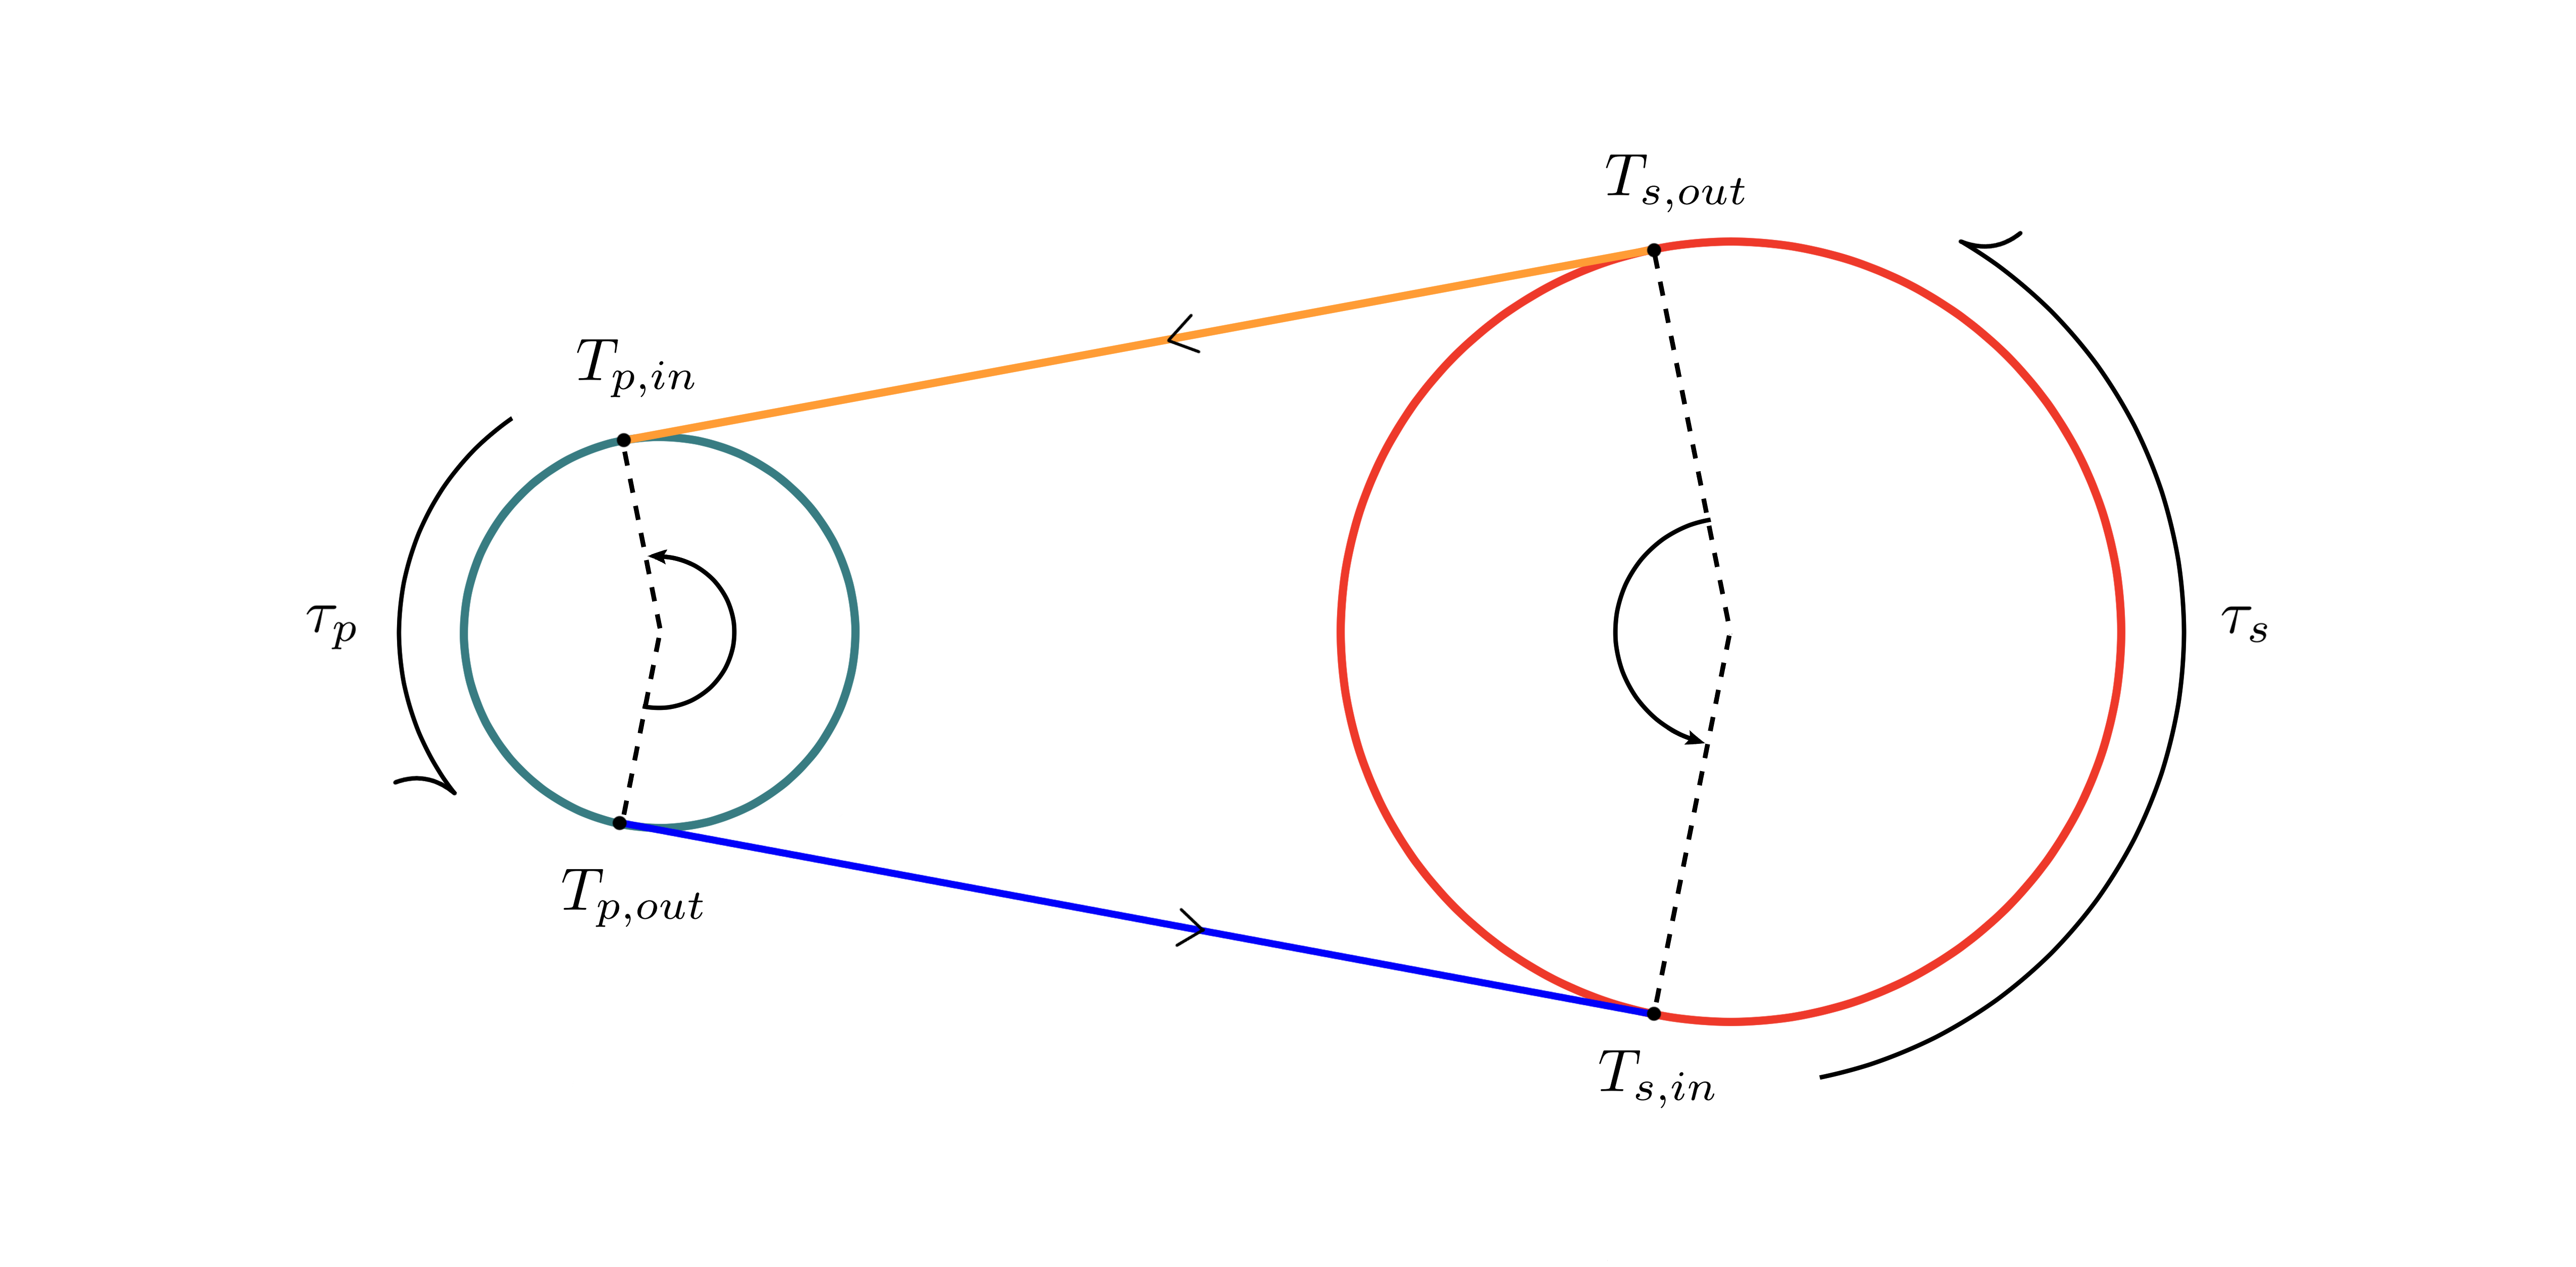
\includegraphics[width=\linewidth]
        {figures/belt/closed_belt_tension_regions.png}
    \caption{
    Complete belt divided into two wrapped regions and two straight spans. The
    arrows show the positive belt-transport direction. The upper span runs
    from the secondary wrap exit, $T_{s,\mathrm{out}}$, to the primary wrap
    entrance, $T_{p,\mathrm{in}}$; the lower span runs from
    $T_{p,\mathrm{out}}$ to $T_{s,\mathrm{in}}$. The torque arrows identify
    the contact actions on the wrapped regions already treated above.
    }
    \label{fig:closed_belt_region_balance}
\end{figure}

As the in--out-of-wrap points move during a shift, each straight span also
rotates. \AssRef{assump:prescribed_belt_path} prescribes this changing path but
explicitly omits the transverse inertia associated with its reorientation.
Accordingly, Newton's second law is applied only along the instantaneous
straight span.

Take this direction as positive with belt travel, and let $p_u$ and $p_l$ be
the tangential momenta of the belt particles occupying the two spans at the
instant considered; Newton's second law follows those same particles. The
downstream tension acts positively and the upstream tension negatively, so

\begin{equation}
\begin{aligned}
    T_{p,\mathrm{in}}-T_{s,\mathrm{out}}
    &=
    \frac{dp_u}{dt},
    \\
    T_{s,\mathrm{in}}-T_{p,\mathrm{out}}
    &=
    \frac{dp_l}{dt}.
\end{aligned}
    \label{eq:straight_span_newton_balances}
\end{equation}

At that instant, a straight span $i\in\{u,l\}$ has mass $\rho_bA_b l_i$.
Under \AssRef{assump:single_belt_speed} and
\AssRef{assump:fixed-belt-cross-section}, its stored tangential momentum is
$p_i=\rho_bA_b l_i v_b$, so the obvious first step is to differentiate:

\[
    \frac{d}{dt}\left(\rho_bA_b l_i v_b\right)
    =
    \rho_bA_b\left(l_i\dot v_b+\dot l_i v_b\right).
\]

The term $\rho_bA_b\dot l_i v_b$ exposes the complication. Each station marks
where the belt enters or leaves the current pulley geometry; it is not fixed
to a particular belt particle. As the stations move, belt particles pass
between the wraps and straight span, so the region contains a changing mass.
The derivative above therefore describes the momentum stored within a moving
region, not yet the material momentum rate required by Newton's second law.
The momentum crossing its boundaries must also be included.

Let $v_i^{-}$ and $v_i^{+}$ denote the velocities of the upstream and
downstream stations, respectively, projected along the straight span. The
belt crosses those boundaries at the relative speeds $v_b-v_i^{-}$ and
$v_b-v_i^{+}$. Adding the outgoing momentum flux and subtracting the incoming
flux gives

\begin{equation}
\begin{aligned}
    \frac{dp_i}{dt}
    ={}&
    \frac{d}{dt}
    \left(
        \rho_bA_b l_i v_b
    \right)
    \\
    &+
    \rho_bA_bv_b
    \left[
        \left(v_b-v_i^{+}\right)
        -
        \left(v_b-v_i^{-}\right)
    \right].
\end{aligned}
    \label{eq:moving_straight_span_momentum_rate}
\end{equation}

These same station velocities determine the changing distance between them:

\begin{equation}
    \dot l_i
    =
    v_i^{+}
    -
    v_i^{-}.
    \label{eq:straight_span_station_kinematics}
\end{equation}

Expanding the stored momentum and substituting
\Cref{eq:straight_span_station_kinematics} gives

\begin{align}
    \frac{dp_i}{dt}
    &={}
    \rho_bA_b
    \left(
        l_i\dot v_b+\dot l_i v_b
    \right)
    +
    \rho_bA_bv_b
    \left(
        v_i^{-}
        -
        v_i^{+}
    \right)
    \notag\\
    &=
    \rho_bA_b
    \left(
        l_i\dot v_b+\dot l_i v_b-\dot l_i v_b
    \right)
    \notag\\
    &=
    \rho_bA_b l_i\dot v_b.
    \label{eq:straight_span_moving_boundary_cancellation}
\end{align}

The cancellation is exact. The station motion changes the momentum stored
within the geometric span by $\rho_bA_b\dot l_i v_b$, but the same motion
produces an equal and opposite momentum flux through its boundaries. Once that
flux is included, the moving stations leave no additional term in the
tangential balance; only the acceleration of the belt transport remains.

The aligned-pulley geometry gives both straight spans the same length $l$, as
shown in \Cref{eq:belt_straight_span_length}. Substituting
\Cref{eq:straight_span_moving_boundary_cancellation} into the two Newton
balances therefore yields

\begin{equation}
\begin{aligned}
    T_{p,\mathrm{in}}-T_{s,\mathrm{out}}
    &=
    \rho_bA_b l\dot v_b,
    \\
    T_{s,\mathrm{in}}-T_{p,\mathrm{out}}
    &=
    \rho_bA_b l\dot v_b.
\end{aligned}
    \label{eq:upper_lower_straight_span_balances}
\end{equation}

Because the right-hand sides of the two straight-span balances are identical,
their tension differences must be equal:

\begin{equation}
    T_{p,\mathrm{in}}-T_{s,\mathrm{out}}
    =
    T_{s,\mathrm{in}}-T_{p,\mathrm{out}}
    \label{eq:straight_span_tension_compatibility}
\end{equation}

Rearranging this result places the two tensions belonging to each pulley on
the same side:

\begin{equation}
    T_{p,\mathrm{in}}+T_{p,\mathrm{out}}
    =
    T_{s,\mathrm{in}}+T_{s,\mathrm{out}}.
    \label{eq:straight_span_boundary_tension_sum}
\end{equation}

The closed belt therefore requires the sum of the primary boundary tensions
to match the sum of the secondary boundary tensions. The remaining task is to
evaluate that sum from the mechanics already obtained for a generic pulley
wrap.

The integrated tangential balance in
\Cref{eq:integrated_wrap_tangential_balance} gives the boundary-tension
difference as

\begin{equation}
    T_{j,\mathrm{out}}-T_{j,\mathrm{in}}
    =
    \rho_bA_b\phi_j
    \left(
        r_{j,\mathrm{cm}}\dot v_b+
        \dot r_jv_b
    \right)
    -\lambda_jN_j.
    \label{eq:generic_wrap_boundary_tension_difference}
\end{equation}

This and the entry-to-exit solution in
\Cref{eq:wrap_entry_exit_tension} are two relations for the same two boundary
tensions. Solving them for the entrance tension gives

\begin{equation}
\begin{aligned}
    T_{j,\mathrm{in}}
    ={}&
    \rho_bA_b
    \left[
        v_b^2-r_{j,\mathrm{cm}}\ddot r_j
        +
        \frac{\sin\beta}{\lambda_j}
        \left(
            r_{j,\mathrm{cm}}\dot v_b+
            \dot r_jv_b
        \right)
    \right]
    \\
    &+
    \frac{
        \lambda_jN_j
        -
        \rho_bA_b\phi_j
        \left(
            r_{j,\mathrm{cm}}\dot v_b+
            \dot r_jv_b
        \right)
    }{
        1-e^{-\frac{\lambda_j}{\sin\beta}\phi_j}
    },
    \qquad \lambda_j\neq0.
\end{aligned}
    \label{eq:generic_wrap_entrance_tension}
\end{equation}

The required sum can now be written as
$2T_{j,\mathrm{in}}+(T_{j,\mathrm{out}}-T_{j,\mathrm{in}})$. Substituting
\Cref{eq:generic_wrap_boundary_tension_difference,eq:generic_wrap_entrance_tension}
and simplifying gives

\begin{equation}
\begin{aligned}
    T_{j,\mathrm{in}}+T_{j,\mathrm{out}}
    ={}&
    2\rho_bA_b
    \left[
        v_b^2-r_{j,\mathrm{cm}}\ddot r_j
        +
        \frac{\sin\beta}{\lambda_j}
        \left(
            r_{j,\mathrm{cm}}\dot v_b+
            \dot r_jv_b
        \right)
    \right]
    \\
    &+
    \frac{
        1+e^{-\frac{\lambda_j}{\sin\beta}\phi_j}
    }{
        1-e^{-\frac{\lambda_j}{\sin\beta}\phi_j}
    }
    \left[
        \lambda_jN_j
        -
        \rho_bA_b\phi_j
        \left(
            r_{j,\mathrm{cm}}\dot v_b+
            \dot r_jv_b
        \right)
    \right],
    \qquad \lambda_j\neq0.
\end{aligned}
    \label{eq:generic_wrap_boundary_tension_sum}
\end{equation}

Applying this expression to the primary and secondary sides of
\Cref{eq:straight_span_boundary_tension_sum} eliminates all four temporary
boundary tensions:

\bigeq{eq:closed_loop_tension_compatibility}
{Closed-Loop Tension Compatibility}
{
\begin{aligned}
    &2\rho_bA_b
    \left[
        v_b^2-r_{p,\mathrm{cm}}\ddot r_p
        +
        \frac{\sin\beta}{\lambda_p}
        \left(
            r_{p,\mathrm{cm}}\dot v_b+
            \dot r_pv_b
        \right)
    \right]
    \\
    &\quad+
    \frac{
        1+e^{-\frac{\lambda_p}{\sin\beta}\phi_p}
    }{
        1-e^{-\frac{\lambda_p}{\sin\beta}\phi_p}
    }
    \left[
        \lambda_pN_p
        -
        \rho_bA_b\phi_p
        \left(
            r_{p,\mathrm{cm}}\dot v_b+
            \dot r_pv_b
        \right)
    \right]
    \\
    &={}
    2\rho_bA_b
    \left[
        v_b^2-r_{s,\mathrm{cm}}\ddot r_s
        +
        \frac{\sin\beta}{\lambda_s}
        \left(
            r_{s,\mathrm{cm}}\dot v_b+
            \dot r_sv_b
        \right)
    \right]
    \\
    &\quad+
    \frac{
        1+e^{-\frac{\lambda_s}{\sin\beta}\phi_s}
    }{
        1-e^{-\frac{\lambda_s}{\sin\beta}\phi_s}
    }
    \left[
        \lambda_sN_s
        -
        \rho_bA_b\phi_s
        \left(
            r_{s,\mathrm{cm}}\dot v_b+
            \dot r_sv_b
        \right)
    \right],
    \qquad \lambda_p\lambda_s\neq0.
\end{aligned}
}

The displayed form assumes nonzero utilization only because the analytical
wrap solution contains factors of $1/\lambda_j$. The zero-utilization limit
remains regular. Using the zero-traction relations from
\Cref{eq:wrap_zero_traction_solution,eq:wrap_normal_resultant_zero_lambda}
gives

\begin{equation}
    T_{j,\mathrm{in}}+T_{j,\mathrm{out}}
    =
    2\rho_bA_b
    \left(
        v_b^2-r_{j,\mathrm{cm}}\ddot r_j
    \right)
    +
    \frac{2N_j\sin\beta}{\phi_j},
    \qquad \lambda_j=0.
    \label{eq:generic_wrap_boundary_tension_sum_zero_lambda}
\end{equation}

This expression replaces the corresponding side of
\Cref{eq:closed_loop_tension_compatibility} whenever $\lambda_p=0$ or
$\lambda_s=0$. The four boundary tensions have therefore disappeared from the
closed-loop equation: the straight spans require the two boundary-tension sums
to match, and the local wrap mechanics express each sum in terms of the pulley
normal load, traction utilization, and retained belt kinematics. Once the
coupled mechanical equations determine those quantities,
\Cref{eq:generic_wrap_entrance_tension,eq:wrap_entry_exit_tension} recover the
boundary tensions and \Cref{eq:wrap_tension_distribution} recovers the tension
through each wrap.

\subsection{Belt-Mechanics Closure and Scope}
\label{sec:belt_mechanics_synthesis}

The closed-loop compatibility in
\Cref{eq:closed_loop_tension_compatibility} is the final relation required
from the belt itself. Rather than fixing the absolute tension level through a
prescribed tight- or slack-side boundary condition, it makes that level
emerge from the two pulley-wrap solutions together with the momentum balances
of the two straight spans. This way of closing the loop also defines the level
of belt resolution retained by the present model.

This treatment combines ideas that more commonly appear at different levels
of resolution. Classical belt relations describe the tension change through a
single wrap once an endpoint tension and contact state are supplied
\citep{Gerbert1996}. Steady whole-belt boundary-value models couple the pulley
contacts and free spans, but typically require operating-point boundary data
such as a prescribed slack-side tension \citep{KongParker2006,Messick2018}.
Transient discretized rubber-belt models instead enforce whole-loop
compatibility through the states of many belt elements
\citep{JulioPlante2011,Ballew2015}. The present formulation occupies a reduced
middle ground: it retains one global belt-transport coordinate and an
analytical closed-loop compatibility without introducing spatial or nodal belt
states.

The chain-CVT model of \citet{DuanEtAl2016} provides the closest comparison
for the retained transient physics. Both formulations account for centripetal
inertia, tangential belt or chain acceleration, and the additional tangential
acceleration produced as the contact radius changes. Duan also couples the
pulley axial and rotational dynamics through the contact solution, as is done
here. One difference is that Duan neglects radial acceleration when reducing
the final spatial wrap equations, whereas the present radial balance retains
it.

Duan resolves considerably more physics within each pulley wrap. The chain
trajectory may depart locally from the nominal pitch circle; radial and
circumferential relative motion determine the sliding direction; friction
varies continuously with sliding speed; and pulley deformation changes the
contact geometry with angular position. Tension and normal loading are
therefore obtained from coupled spatial equations. In the present model,
\AssRef{assump:prescribed_belt_path} fixes a circular contact path on rigid
pulley geometry, \AssRef{assump:single_belt_speed} assigns one transport speed
to the belt, and \AssRef{assump:wrap_contact_resolution} assigns one traction
utilization \(\lambda_j\) to each wrap. The present formulation consequently
retains the mechanism-level transient dynamics while sacrificing within-wrap
variation of migration, microslip, traction reversal, and pulley deformation.

The complete belt loop is also closed differently. Duan concentrates the
chain's longitudinal deformation in the tight span, obtains its absolute
tension from a lumped spring--damper law, and assumes that tension is equal at
the driving-pulley entrance and driven-pulley exit. The tension difference
across the slack span then accelerates the mass of the complete chain. Under
\AssRef{assump:constant_belt_length}, the present formulation has no
longitudinal stretch law from which to obtain an absolute tension. Instead,
both straight spans are treated as massive belt regions, including the
momentum carried through their moving in--out-of-wrap boundaries. Combining
those balances with the two wrap solutions closes the loop without prescribing
a tight- or slack-side tension.

The comparison is therefore best understood as a difference in where each
model places its resolution. Duan resolves the local contact, friction, chain
elasticity, and pulley deformation in greater detail. The present formulation
uses a coarser contact description, but carries radial acceleration, both
straight-span inertias, moving-boundary momentum transport, movable-sheave
dynamics, and pulley rotation through the complete belt loop. The distributed
tangential action within each wrap is reduced to the single signed utilization
\(\lambda_j\), allowing these mechanism-level transients to be retained
without introducing a spatially discretized belt state.

\section{Tangential Contact-State Closure}
\label{sec:engaged_dynamic_closure}

The fully engaged CVT has now been followed through every retained motion and
free body. \Cref{sec:geometry} relates the sheave positions and pulley radii,
\Cref{sec:axial_actuation_balances} balances the two movable assemblies,
\Cref{sec:pulley_rotational_dynamics} balances the two rotating assemblies,
and \Cref{sec:belt_transport_contact} balances the belt around both wraps and
straight spans. No additional free body or degree of freedom remains to be
introduced.

Looking across those relations, only two quantities remain without relations
that fix their values at the current instant: \(\lambda_p\) and
\(\lambda_s\). The reason lies in how \(\lambda_j\) was introduced in
\Cref{eq:lambda_local_definition}. There, the separate Coulomb conditions on
traction magnitude, direction, and whether the contact is sticking or sliding
were collected into the single signed utilization \(\lambda_j\). That
compression let the remainder of the belt derivation carry one contact
quantity through the wrap tension, normal loading, pulley torque, and
closed-loop belt relations without reopening the piecewise contact law at
every step.

Importantly, this is different from adding one more balance. The equations
derived so far keep the same form as the CVT moves. Changing a belt--pulley
contact between sticking and sliding, however, is a change of mechanical
regime: the actual relation used to determine \(\lambda_j\) changes with the
contact state. This is the type of regime change introduced in
\Cref{sec:mechanical_regimes_state_evolution}, where a change in the active
contact or constraint state changes the equations governing the mechanism.
What remains is therefore not another motion or free-body balance, but the 
choice of which tangential contact relation governs each wrap.

% --------------------------------------------------------------
\subsection{Relative Motion at the Pulley Contacts}
\label{sec:tangential_contact_states}

With the remaining ambiguity reduced to the two Coulomb branches, the first
useful distinction is the contact motion itself. Sticking and sliding differ
in whether the belt has relative tangential motion with respect to the pulley
contact represented by a wrap. Before that relative motion can be written, the
surface speed represented by each reduced contact must therefore be identified.

For the primary, this comparison is direct. Both sheave faces rotate with the
primary shaft, so their angular speed is \(\omega_p\). The secondary is
different. Under \AssRef{assump:wrap_contact_resolution}, the complete wrap
carries one traction state rather than separate states for the fixed and
movable faces, while the helix kinematics already established that the two
physical faces do not generally have the same speed during a shift. The fixed
face rotates at \(\omega_s\), whereas
\Cref{eq:secondary_movable_sheave_speed} gives the movable-face speed
\(\omega_{s,M}=\omega_s+\dot\theta_s\).

One representative secondary surface speed is therefore required. Its value
is fixed by the same face-torque reduction already used in
\AssRef{assump:symmetric_face_sharing}. In particular,
\Cref{eq:secondary_movable_face_belt_torque} gives
\(\tau_{s,M}=\tau_s/2\), and therefore
\(\tau_{s,F}=\tau_s/2\). The instantaneous power delivered by the belt
torque to the two faces is

\begin{equation}
\begin{aligned}
    P_{s,\mathrm{faces}}
    &=
    \tau_{s,F}\omega_s
    +
    \tau_{s,M}\omega_{s,M}
    \\
    &=
    \frac{\tau_s}{2}\omega_s
    +
    \frac{\tau_s}{2}
    \left(\omega_s+\dot\theta_s\right)
    \\
    &=
    \tau_s
    \left(
        \omega_s+\frac{1}{2}\dot\theta_s
    \right).
\end{aligned}
\label{eq:secondary_face_tangential_power}
\end{equation}

Let \(\bar\omega_s\) be the angular speed assigned to the single aggregate
secondary contact. The same total torque represented by that contact carries
power \(\tau_s\bar\omega_s\). Equating this power with
\Cref{eq:secondary_face_tangential_power} fixes the representative speed. The
primary and secondary contact speeds can therefore be written together as

\begin{equation}
\boxed{
    \bar\omega_p=\omega_p,
    \qquad
    \bar\omega_s
    =
    \omega_s+\frac{1}{2}\dot\theta_s
    =
    \frac{\omega_s+\omega_{s,M}}{2}.
}
\label{eq:representative_contact_angular_speed}
\end{equation}

Thus the average in \Cref{eq:representative_contact_angular_speed} is not an
additional empirical approximation. Once one secondary traction state and the
equal face-torque split have been adopted, power consistency selects this
representative surface speed. The arithmetic mean appears specifically because the
two torque shares are equal. It remains an aggregate quantity: the model still
does not determine the separate sliding states of the fixed and movable faces.

Returning now to relative motion, look at pulley \(j\). The belt moves through
the wrap with signed transport speed \(v_b\), while the represented pulley surface 
moves tangentially at \(r_{j,\mathrm{eff}}\bar\omega_j\). Their difference defines 
the relative tangential speed,

\begin{equation}
    v_{\mathrm{rel},j}
    =
    v_b-r_{j,\mathrm{eff}}\bar\omega_j,
    \qquad
    j\in\{p,s\}.
\label{eq:tangential_relative_speed}
\end{equation}

The sign follows the common belt-transport and rotational directions defined
in \Cref{sec:rotational_sign}. Positive \(v_{\mathrm{rel},j}\) means the belt
moves ahead of the represented pulley contact in the positive belt direction,
while a negative value means it moves the other way.

If \(v_{\mathrm{rel},j}\neq0\), the contact is already sliding. Its relative
motion fixes the direction of friction, and kinetic Coulomb friction fixes the
magnitude. The sliding branch of \Cref{eq:lambda_local_definition} therefore
gives

\begin{equation}
\begin{aligned}
    \sigma_j
    &=
    -\operatorname{sgn}\!\left(v_{\mathrm{rel},j}\right),
    \\
    \lambda_j
    &=
    \sigma_j\mu_k,
    \qquad
    v_{\mathrm{rel},j}\neq0.
\end{aligned}
\label{eq:sliding_traction_utilization}
\end{equation}

Sliding therefore closes \(\lambda_j\) directly from the current contact
motion. Sticking begins at the opposite kinematic condition,

\begin{equation}
    v_{\mathrm{rel},j}=0
    \qquad\Longleftrightarrow\qquad
    v_b=r_{j,\mathrm{eff}}\bar\omega_j.
\label{eq:sticking_velocity_compatibility}
\end{equation}

The important point is that zero relative speed does not imply zero tangential
force. It only says that the belt and represented pulley contact move together
at that instant. Static friction may still supply a nonzero reaction, with
\(\lambda_j\) taking whatever signed value is required to maintain sticking
so long as the static limit in \Cref{eq:lambda_local_definition} is not
exceeded.

That speed match must also persist. If the belt speed and represented
pulley-surface speed begin changing at different rates, relative motion appears
immediately. Differentiating
\Cref{eq:representative_contact_angular_speed} gives

\begin{equation}
\begin{aligned}
    \dot{\bar\omega}_p
    &=
    \dot\omega_p,
    \\
    \dot{\bar\omega}_s
    &=
    \dot\omega_s+\frac{1}{2}\ddot\theta_s
    \\
    &=
    \dot\omega_s
    +
    \frac{1}{2}
    \left[
        \frac{d\theta_s}{dx_s}\ddot x_s
        +
        \frac{d^2\theta_s}{dx_s^2}\dot x_s^2
    \right],
\end{aligned}
\label{eq:representative_contact_angular_acceleration}
\end{equation}

where the final line follows directly from
\Cref{eq:secondary_movable_sheave_acceleration}. Differentiating
\Cref{eq:tangential_relative_speed} then gives the relative tangential
acceleration,

\begin{equation}
\begin{aligned}
    a_{\mathrm{rel},j}
    &\equiv
    \dot v_{\mathrm{rel},j}
    \\
    &=
    \dot v_b
    -
    r_{j,\mathrm{eff}}\dot{\bar\omega}_j
    -
    \dot r_{j,\mathrm{eff}}\bar\omega_j .
\end{aligned}
\label{eq:tangential_relative_acceleration}
\end{equation}

The first two terms are the direct comparison between belt acceleration and
the acceleration of a represented pulley surface at fixed radius. The final term appears
because the contact radius is not fixed during a shift. As established in
\Cref{eq:radial_reference_rate_equivalence}, the effective radius moves with
the pulley radius, so \(r_{j,\mathrm{eff}}\omega_j\) can change even when
\(\omega_j\) is momentarily constant. A sticking belt must follow that change
as well.

Established sticking therefore requires

\begin{equation}
    a_{\mathrm{rel},j}=0.
\label{eq:sticking_acceleration_compatibility}
\end{equation}

The two Coulomb branches now leave different things to determine. Sliding
already supplies \(\lambda_j\). Sticking instead supplies the condition that
the mechanics must satisfy, \(a_{\mathrm{rel},j}=0\), while \(\lambda_j\)
remains the static reaction required to make that condition hold within the
available friction limit.

\subsection{Determining the Sticking Traction}
\label{sec:sticking_traction_closure}

For a sticking contact, the previous subsection leaves a simple-looking pair:
\(\lambda_j\) is unknown, while the contact must satisfy
\(a_{\mathrm{rel},j}=0\). At first, this seems no different from any other
unknown and equation already added to the model. If \(\lambda_j\) entered the
mechanics linearly, it could simply be solved algebraically alongside the
other instantaneous unknowns.

Whether that is possible can be read directly from the equations already
derived. The pulley torque in \Cref{eq:generic_belt_contact_torque}, for
example, contains

\begin{equation}
    \tau_j
    =
    -r_{j,\mathrm{eff}}\lambda_jN_j,
\label{eq:sticking_closure_contact_product}
\end{equation}

so an unknown \(\lambda_j\) multiplies the unknown normal resultant \(N_j\).
The equation is therefore no longer linear in the unknowns. If this product
were the only complication, however, another rearrangement might still isolate
\(\lambda_j\). The stronger obstacle comes from the wrap relation carried into
the closed-loop belt compatibility. Through
\Cref{eq:generic_wrap_boundary_tension_sum}, the same \(\lambda_j\) also
appears reciprocally and inside terms such as

\begin{equation}
    \frac{\sin\beta}{\lambda_j},
    \qquad
    \frac{
        1+e^{-\frac{\lambda_j\phi_j}{\sin\beta}}
    }{
        1-e^{-\frac{\lambda_j\phi_j}{\sin\beta}}
    }.
\label{eq:sticking_closure_nonlinear_terms}
\end{equation}

With the same unknown appearing both
in products with other unknowns and inside reciprocal and exponential terms,
there is no useful algebraic rearrangement that isolates the required static
utilization.

There is one important simplification. This nonlinear dependence comes from
the unknown static \(\lambda_j\) itself; the other remaining accelerations and
contact loads appear linearly. If the static utilization were known, those
quantities could be obtained directly from the balances already derived.

That suggests turning the problem around. Rather than trying to isolate
\(\lambda_j\) explicitly, choose a candidate static utilization and determine
the response it would produce. The resulting accelerations give
\(a_{\mathrm{rel},j}\) through
\Cref{eq:tangential_relative_acceleration}. Since sticking requires the
relative acceleration to vanish, \(a_{\mathrm{rel},j}\) can be used directly
as the residual for the static-traction solve,

\begin{equation}
    a_{\mathrm{rel},j}=0.
\label{eq:sticking_traction_root_condition}
\end{equation}

This is the same basic idea used for the geometric compatibility roots in
\Cref{sec:geometry}. A nonzero residual means that the candidate traction
would make the belt and pulley surface begin accelerating relative to one
another. The required static utilization is the value for which the residual
vanishes. Finding that value is therefore a root solve in the unknown static
traction.

If only one wrap is sticking, the other utilization is already fixed by its
sliding branch. One static \(\lambda_j\) and one sticking residual remain, so
the root is one-dimensional. If both wraps are sticking, the two static
utilizations influence the same mechanical response and must be varied
together until both residuals vanish,

\begin{equation}
    a_{\mathrm{rel},p}(\lambda_p,\lambda_s)=0,
    \qquad
    a_{\mathrm{rel},s}(\lambda_p,\lambda_s)=0.
\label{eq:stick_stick_root_condition}
\end{equation}

This leaves only a one- or two-dimensional nonlinear search in the static
traction utilizations. For each candidate value or pair, everything else is
obtained from the linear balances already derived.

\subsection{The Common Mechanical Solve}
\label{sec:engaged_mechanical_core}

The two contact branches now reduce to the same mechanical calculation.
Sliding supplies \(\lambda_j\) directly, while sticking tests candidate values
as its root is found. In either case, evaluating the instantaneous response
begins with one traction utilization for each wrap. The remaining step is to
solve the mechanics for that pair.

With \(\lambda_p\) and \(\lambda_s\) specified, the equations already
derived can now be read simply for the quantities they still have to
determine. The axial balances expose the first of these unknowns. The primary balance in
\Cref{eq:primary_balance_in_shift_coordinate} relates the shared shift
acceleration \(\ddot s\) to the primary normal resultant \(N_p\). The
secondary balance in \Cref{eq:secondary_balance_in_shift_coordinate} contains
the same \(\ddot s\), the secondary normal resultant \(N_s\), and also the
secondary shaft acceleration \(\dot\omega_s\) and belt torque \(\tau_s\).

The rotational balances add the shaft dynamics. The primary and secondary
relations in
\Cref{eq:primary_rotational_eom_belt,eq:secondary_rotational_eom_belt}
contain \(\dot\omega_p\) and \(\dot\omega_s\), together with the belt torques
\(\tau_p\) and \(\tau_s\); the secondary relation also contains the same
\(\ddot s\) through the helix kinematics. The torques may look like two more
unknowns, but the specified traction pair removes them immediately. From
\Cref{eq:generic_belt_contact_torque},

\begin{equation}
    \tau_j
    =
    -r_{j,\mathrm{eff}}\lambda_jN_j,
    \qquad
    j\in\{p,s\},
\end{equation}

so each pulley torque is set by the same normal resultant already appearing in
the axial balances.

The complete-belt transport balance in
\Cref{eq:complete_belt_transport_newton} brings in the belt acceleration
\(\dot v_b\). Its two tangential pulley actions are again the belt torques, so
after the relation above is substituted the transport equation involves
\(\dot v_b\), \(N_p\), and \(N_s\) for the specified traction pair.

Finally, the closed-loop tension compatibility in
\Cref{eq:closed_loop_tension_compatibility} relates the same belt acceleration
and normal resultants to the radial accelerations of the two wraps. Those
radial accelerations introduce no new degree of freedom:
\Cref{eq:primary_radius_acceleration,eq:secondary_radius_acceleration} already
express them in terms of the current geometry, \(\dot s\), and the same shift
acceleration \(\ddot s\). The four temporary boundary tensions have likewise
already disappeared from the closed-loop relation.

No new unknown appears as these equations are brought together. The quantities
left to determine are exactly

\begin{equation}
    \mathbf z
    =
    \begin{bmatrix}
        \dot\omega_p &
        \dot\omega_s &
        \dot v_b &
        \ddot s &
        N_p &
        N_s
    \end{bmatrix}^{\mathsf T}.
\label{eq:engaged_linear_unknowns}
\end{equation}

At this point, every other term in the six equations is fixed by the current
state, the specified traction pair, and the component relations already
derived. Each equation is also linear in the six entries of \(\mathbf z\).
Collecting them therefore gives

\begin{equation}
    \mathbf A(\lambda_p,\lambda_s)\mathbf z
    =
    \mathbf b(\lambda_p,\lambda_s).
\label{eq:engaged_six_by_six_mechanical_core}
\end{equation}

To write \(\mathbf A\) and \(\mathbf b\) out cleanly, a small amount of
temporary notation is useful. For this matrix only, primes shorten
derivatives: \(x_s'\), \(r_j'\), \(q_f'\), and \(J_{f,p}'\) denote
derivatives with respect to \(s\), while \(\theta_s'\) denotes
differentiation with respect to \(x_s\); double primes follow the same
convention. The only additional symbols are the two analytical wrap factors
repeated in the closed-loop row,

\begin{equation}
\begin{aligned}
    \mathcal C_{v,j}
    &\equiv
    \begin{cases}
        \displaystyle
        \frac{2\sin\beta}{\lambda_j}
        -
        \phi_j
        \frac{
            1+e^{-\frac{\lambda_j\phi_j}{\sin\beta}}
        }{
            1-e^{-\frac{\lambda_j\phi_j}{\sin\beta}}
        },
        & \lambda_j\neq0,
        \\[8pt]
        0,
        & \lambda_j=0,
    \end{cases}
    \\[8pt]
    \mathcal C_{N,j}
    &\equiv
    \begin{cases}
        \displaystyle
        \lambda_j
        \frac{
            1+e^{-\frac{\lambda_j\phi_j}{\sin\beta}}
        }{
            1-e^{-\frac{\lambda_j\phi_j}{\sin\beta}}
        },
        & \lambda_j\neq0,
        \\[8pt]
        \displaystyle
        \frac{2\sin\beta}{\phi_j},
        & \lambda_j=0.
    \end{cases}
\end{aligned}
\label{eq:engaged_wrap_matrix_coefficients}
\end{equation}

These two symbols are temporary assembly notation only. Their
\(\lambda_j=0\) branches are the finite limits already established in
\Cref{eq:generic_wrap_boundary_tension_sum_zero_lambda}.

The coefficient matrix is then

\begin{equation}
\resizebox{0.98\textwidth}{!}{$
\mathbf A
=
\begin{bmatrix}
I_{\mathrm B,p}+I_{p,\mathrm{const}}+J_{f,p}
&0
&0
&0
&r_{p,\mathrm{eff}}\lambda_p
&0
\\
0
&I_{\mathrm B,s}+I_{s,F}+I_{s,M}
&0
&I_{s,M}\theta_s'x_s'
&0
&r_{s,\mathrm{eff}}\lambda_s
\\
0
&0
&0
&m_p+I_f(q_f')^2
&\tfrac12\cos\beta
&0
\\
0
&I_{s,M}\theta_s'
&0
&\bigl[m_s+I_{s,M}(\theta_s')^2\bigr]x_s'
&0
&\tfrac12
 \bigl(
    \cos\beta+r_{s,\mathrm{eff}}\lambda_s\theta_s'
 \bigr)
\\
0
&0
&m_b
&0
&-\lambda_p
&-\lambda_s
\\
0
&0
&\rho_bA_b
 \bigl(
    r_{p,\mathrm{cm}}\mathcal C_{v,p}
    -
    r_{s,\mathrm{cm}}\mathcal C_{v,s}
 \bigr)
&2\rho_bA_b
 \bigl(
    r_{s,\mathrm{cm}}r_s'
    -
    r_{p,\mathrm{cm}}r_p'
 \bigr)
&\mathcal C_{N,p}
&-\mathcal C_{N,s}
\end{bmatrix}
$}.
\label{eq:engaged_mechanical_matrix}
\end{equation}

The corresponding known-side vector is

\begingroup
\small
\begin{equation}
\mathbf b
=
\begin{bmatrix}
\displaystyle
\tau_{\mathrm B,p}
-
J_{f,p}'\dot s\,\omega_p
\\[9pt]
\displaystyle
\tau_{\mathrm B,s}
-
I_{s,M}
\bigl[
    \theta_s'x_s''
    +
    \theta_s''(x_s')^2
\bigr]\dot s^2
\\[9pt]
\displaystyle
\frac12\omega_p^2J_{f,p}'
-
I_fq_f'q_f''\dot s^2
-
k_p(x_{p,\mathrm{pre}}+s)
\\[9pt]
\displaystyle
\theta_s'k_{s,\theta}
(\theta_{s,\mathrm{pre}}-\theta_s)
+
k_{s,x}(x_{s,\mathrm{pre}}-x_s)
-
\Bigl\{
    \bigl[m_s+I_{s,M}(\theta_s')^2\bigr]x_s''
    +
    I_{s,M}\theta_s'\theta_s''(x_s')^2
\Bigr\}\dot s^2
\\[9pt]
0
\\[9pt]
\displaystyle
2\rho_bA_b
\bigl(
    r_{p,\mathrm{cm}}r_p''
    -
    r_{s,\mathrm{cm}}r_s''
\bigr)\dot s^2
+
\rho_bA_bv_b
\bigl(
    \dot r_s\mathcal C_{v,s}
    -
    \dot r_p\mathcal C_{v,p}
\bigr)
\end{bmatrix}.
\label{eq:engaged_mechanical_rhs}
\end{equation}
\endgroup

The row order follows the derivation: the first two rows are the pulley
rotational balances, the next two are the axial balances, the fifth is the
complete-belt transport balance, and the sixth is the closed-loop tension
compatibility.

For a specified traction pair, every entry of \(\mathbf A\) and
\(\mathbf b\) is fixed by the current state and the component relations already
derived. Solving \Cref{eq:engaged_six_by_six_mechanical_core} then gives the
two shaft accelerations, belt acceleration, shift acceleration, and the two
normal resultants. A sliding \(\lambda_j\) reaches this solve directly from
kinetic friction; a sticking \(\lambda_j\) reaches the same solve as a
candidate value whose resulting \(a_{\mathrm{rel},j}\) is returned to the
root described in \Cref{sec:sticking_traction_closure}.

The four contact combinations can now be read off directly:

\begin{center}
\small
\renewcommand{\arraystretch}{1.35}
\begin{tabular}{c|p{0.34\textwidth}|p{0.34\textwidth}}
    &
    \textbf{Secondary sliding}
    &
    \textbf{Secondary sticking}
    \\ \hline

    \textbf{Primary sliding}
    &
    Both \(\lambda_p\) and \(\lambda_s\) are fixed by kinetic friction.
    One \(6\times6\) solve gives the instantaneous response.
    &
    \(\lambda_p\) is fixed by kinetic friction, while \(\lambda_s\) is found
    from the one-dimensional root \(a_{\mathrm{rel},s}=0\). Each candidate
    \(\lambda_s\) is evaluated through the same \(6\times6\) solve.
    \\ \hline

    \textbf{Primary sticking}
    &
    \(\lambda_s\) is fixed by kinetic friction, while \(\lambda_p\) is found
    from the one-dimensional root \(a_{\mathrm{rel},p}=0\). Each candidate
    \(\lambda_p\) is evaluated through the same \(6\times6\) solve.
    &
    \(\lambda_p\) and \(\lambda_s\) are found together from
    \(a_{\mathrm{rel},p}=0\) and \(a_{\mathrm{rel},s}=0\). Each candidate
    pair is evaluated through the same \(6\times6\) solve.
\end{tabular}
\end{center}

The six mechanical balances are therefore common to all four cases. What
changes with the contact regime is only how the traction pair supplied to
those balances is obtained: directly from kinetic friction, from one
static-traction root, or from the two sticking conditions together.

\subsection{Contact Admissibility and Regime Transitions}
\label{sec:contact_admissibility_transitions}

The four contact combinations above are enough to obtain an instantaneous
response for any assumed tangential regime. They do not yet tell us whether
that regime can actually be maintained, or what should happen when it cannot.

For a sticking contact, \(\lambda_j\) is the static reaction required to keep
the belt and pulley moving together, as introduced in
\Cref{eq:lambda_local_definition}. The root in
\Cref{sec:sticking_traction_closure} finds the value of that reaction that
satisfies \(a_{\mathrm{rel},j}=0\). Sticking is physically available only while the
required reaction lies within the static Coulomb limit,

\begin{equation}
    \left|\lambda_j\right|\leq\mu_s .
\label{eq:sticking_admissibility}
\end{equation}

If this condition is satisfied, the contact can supply the traction needed to
remain stuck. If the required \(\left|\lambda_j\right|\) would exceed
\(\mu_s\), no admissible static reaction can preserve zero relative motion and
the sticking regime must end.

Sliding is simpler away from zero relative speed. While
\(v_{\mathrm{rel},j}\neq0\), its sign identifies the sliding direction and
\Cref{eq:sliding_traction_utilization} fixes the corresponding kinetic
traction. The next ambiguity appears only when \(v_{\mathrm{rel},j}\) reaches
zero. At that instant the belt and pulley are momentarily moving together, so
the first possibility to test is sticking. The required static
\(\lambda_j\) is found from \(a_{\mathrm{rel},j}=0\) and checked against
\Cref{eq:sticking_admissibility}. If it is admissible, the contact captures
into sticking.

If sticking is not admissible, the contact must leave
\(v_{\mathrm{rel},j}=0\) on a sliding branch. For a contact that arrived at
zero while already sliding, two continuations are possible: the relative
velocity may grow again in the same direction as before, or the sliding
direction may reverse and grow in the opposite direction. At the event itself,
\(v_{\mathrm{rel},j}=0\), so the relative velocity cannot distinguish between
those two possibilities. The relative acceleration does: its sign tells which
way \(v_{\mathrm{rel},j}\) begins to move away from zero.

For a candidate kinetic sign \(\sigma_j\), consistency therefore requires

\begin{equation}
    \sigma_j\,a_{\mathrm{rel},j}<0,
    \qquad
    v_{\mathrm{rel},j}=0,
\label{eq:sliding_onset_sign_consistency}
\end{equation}

because \(\sigma_j\) is defined opposite to the direction of sliding. The
valid kinetic branch is the one whose solved acceleration produces the
relative-motion direction assumed by that branch. The same check selects the
initial sliding direction when a sticking contact first releases.

Together, these checks also make the order of a regime update clear. Consider a
sliding--sliding solution in which the primary relative velocity reaches zero.
The secondary contact can initially be left on its current kinetic branch
while the primary is tested as sticking. If the required static
\(\lambda_p\) is admissible, the candidate regime becomes
sticking--sliding. If it is not, the primary remains sliding and the kinetic
branch consistent with
\Cref{eq:sliding_onset_sign_consistency} is selected instead. The resulting
traction pair changes the common mechanical response, so that response is
solved again and the contact conditions at both wraps are checked once more.
If both contacts reach a regime boundary at the same instant, the same logic
is applied to the combined candidate regime rather than updating the two wraps
independently.

These tangential contact changes are nonimpulsive regime transitions in the
sense introduced in \Cref{sec:mechanical_regimes_state_evolution}. The belt
and pulley reach the event with continuous position and velocity; changing the
active contact law changes the acceleration that follows rather than resetting
the state instantaneously. The remaining structural regime changes associated
with engagement and shift boundaries require a separate treatment.

\section{Shift-Regime Dynamics and Boundary Transitions}
\label{sec:shift_regime_dynamics}

The freely shifting engaged CVT is now mechanically closed.
For any admissible tangential contact regime,
\Cref{sec:engaged_dynamic_closure} determines how the pulley speeds,
belt transport, and shift coordinate evolve from the current state.
But that solution does more than describe the mechanism at one instant:
as it is integrated forward in time, it moves the hardware.

Consider what that motion can do.
Continued backshift closes the secondary until it can move no farther;
continued primary opening can then separate the primary sheave from the belt.
In the opposite direction, continued upshift eventually carries the primary
to the end of its closing travel.
The equations developed so far can bring the CVT to each of these configurations,
but once one is reached, the physical problem has changed.
A sheave that was free to move may now be supported by a stop,
or a belt--sheave interaction that previously transmitted force may no longer exist.

Reaching one of these boundaries therefore changes the shift regime of the CVT,
in the same sense that a change between sticking and sliding changes a tangential contact regime
in \Cref{sec:engaged_dynamic_closure}.
That structural change has two separate consequences.
First, the active contacts, supports, and permitted motions are different,
so the continuous governing equations must change with the regime.
Second, the state arriving at the boundary may contain a velocity that the new regime
cannot support, so the incoming motion must be transferred into a compatible outgoing state.

These are different mechanical problems.
The first determines how the CVT accelerates once the new regime is active.
The second determines how its velocity changes at the instant the regime is entered.
Both are required if the model is to pass through a shift-regime boundary
without replacing the mechanics by an imposed reset.

\subsection{Shift Domain and Structural Regimes}
\label{sec:shift_coordinate_boundaries}

Before the governing equations can change with the shift regime,
the boundaries between those regimes must first be located along the shift motion.
The shift coordinate already traces the primary through its full travel, so the
geometry derived in \Cref{sec:geometry} identifies where contact is gained or
lost, where hardware begins to support the motion, and which arrangement exists
on either side of each boundary. Following the primary from fully open to fully
closed makes those changes explicit.

Consider first the primary closing during engaged upshift. Its groove
narrows, moving the belt outward. The fixed belt length requires the secondary
radius to decrease, so the secondary opens. This motion can continue until
the primary reaches its closing stop at \(x_p=x_{p,\max}\). Further upshift
would require the primary to close farther, into the stop. The belt remains
between both pairs of sheave faces, so the mechanism can be held at this
ratio with both pulley contacts present.

Opening the primary reverses these motions. The belt moves inward on the
primary and outward on the secondary, bringing the secondary toward its
fully closed stop. The secondary reaches that stop when the primary is at
\(x_p=x_{p,\mathrm{dz}}\), as given by
\Cref{eq:secondary_coordinate_map}. Now try to continue the same engaged
backshift: the belt would have to move farther outward on the secondary,
which would require its sheave to close beyond the stop. With shift motion
at rest and primary belt contact maintained, the secondary stop can therefore
hold the mechanism at its minimum ratio. This is the
\emph{engaged low-ratio seat}.

Yet the primary has not reached its own opening stop. Its groove can open
wider than the belt, leaving the clearance introduced in
\Cref{eq:primary_local_radius_map}. The primary can therefore open farther
if it separates from the belt. That opening no longer moves the belt inward
or requires the secondary to close farther. Under the deadzone mapping, the
secondary stays fully closed and both prescribed belt radii remain fixed
while the primary crosses its clearance. Only when the primary reaches
\(x_p=0\) does its own opening stop prevent further travel.

The secondary stop thus limits the engaged backshift before the primary
exhausts its opening travel. Closing the primary through the same clearance
first brings it back to the belt; further closure then moves the belt outward
and opens the secondary away from its stop.

Since \(s\equiv x_p\) by \Cref{eq:system_shift_coordinate}, the same travel
and boundary positions in the generalized shift coordinate are

\begin{equation}
    0\leq s\leq s_{\max},
    \qquad
    s_{\mathrm{dz}}\equiv x_{p,\mathrm{dz}},
    \qquad
    s_{\max}\equiv x_{p,\max}.
    \label{eq:shift_operating_domain}
\end{equation}

These motions divide the full primary travel into the five structural
arrangements summarized in
\Cref{tab:shift_structural_arrangements}.

\begin{table}[H]
    \centering
    \small
    \renewcommand{\arraystretch}{1.18}
    \begin{tabular}{@{}
        >{\raggedright\arraybackslash}p{0.24\linewidth}
        >{\raggedright\arraybackslash}p{0.18\linewidth}
        >{\raggedright\arraybackslash}p{0.48\linewidth}
        @{}}
        \toprule
        \textbf{Structural regime}
        & \textbf{Primary belt contact}
        & \textbf{Axial motion or support}
        \\
        \midrule
        Fully open primary stop
        & Absent
        & Primary held at \(s=0\); secondary remains fully closed.
        \\[4pt]
        Free deadzone
        & Absent
        & Primary free for \(0<s<s_{\mathrm{dz}}\); secondary remains
          fully closed.
        \\[4pt]
        Engaged low-ratio seat
        & Present
        & Fully closed secondary stop holds the engaged mechanism at
          \(s=s_{\mathrm{dz}}\).
        \\[4pt]
        Free engaged shift
        & Present
        & Free shift for \(s_{\mathrm{dz}}<s<s_{\max}\); both sheaves
          follow the belt geometry.
        \\[4pt]
        Engaged upper primary stop
        & Present
        & Primary closing stop holds the engaged mechanism at
          \(s=s_{\max}\).
        \\
        \bottomrule
    \end{tabular}
    \caption{Structural arrangements over the primary travel. The secondary
    retains belt contact in all five arrangements.}
    \label{tab:shift_structural_arrangements}
\end{table}

A boundary position does not, by itself, determine which shift regime
is active. At \(s=s_{\mathrm{dz}}\), the secondary may be held against its
fully closed stop while the primary remains in contact with the belt. The
primary may instead begin closing, opening the secondary away from that stop,
or it may begin opening and separate from the belt into the clearance. All
three continuations pass through the same value of \(s\). What changes is
which contacts and supports are active and which motions they permit. The
shift regime must therefore be carried as part of the mechanical
description; it cannot be inferred from the shift coordinate alone. This is
the same regime-dependent logic introduced in
\Cref{sec:mechanical_regimes_state_evolution}, now applied to the changing
mechanical arrangement of the CVT.

The same boundary also shows that shift regime and tangential contact
state describe different parts of the mechanics. While the secondary stop
holds the engaged mechanism at \(s=s_{\mathrm{dz}}\), the two shafts and the
belt can continue moving. The stop determines whether further axial motion is
available, but it does not determine whether the belt sticks to either pulley
or slides relative to it. Each engaged shift regime must therefore still
be combined with the corresponding tangential contact regimes from
\Cref{sec:engaged_dynamic_closure}.

The three boundary positions and the five arrangements in
\Cref{tab:shift_structural_arrangements} therefore define where structural
regime changes may occur and which arrangements are physically admissible
there. They do not assign a unique regime to each value of \(s\); at a shared
boundary, the active contacts, supports, and direction of continuation still
matter. The active shift regime and tangential contact regimes together specify
the mechanical regime that the model must track as the CVT evolves.

% ---------------------------------------------------------------------------

\subsection{Governing Equations in Each Shift Regime}
\label{sec:structural_regime_governing_equations}

Knowing which shift regime is active tells us which contacts and supports exist,
but it does not yet determine how the CVT moves within that regime. The
continuous equations must reflect those physical conditions. The useful
starting point is the mechanical system already assembled for free engaged
motion in \Cref{eq:engaged_six_by_six_mechanical_core}. Its six rows are the
primary and secondary rotational balances, the primary and secondary axial
balances, the complete-belt transport balance, and the closed-loop tension
compatibility. A different shift regime does not require these mechanics to be
derived again. It changes which of those balances remain active, which contact
terms disappear, and which motions are prescribed by the hardware.

\subsubsection{Disengaged Primary and Deadzone Motion}
\label{sec:deadzone_continuous_regimes}

At the fully open end of travel, the primary sheaves do not touch the belt,
and the same remains true while the primary crosses the clearance toward
\(s=s_{\mathrm{dz}}\). The immediate consequence is

\begin{equation}
    N_p=0,
    \qquad
    \tau_p=0.
    \label{eq:deadzone_primary_disengaged}
\end{equation}

Putting this contact loss back into the assembled mechanics shows exactly what
changes on the primary side. The rotational balance in
\Cref{eq:primary_rotational_eom_belt} and the axial balance in
\Cref{eq:primary_balance_in_shift_coordinate} still describe the same primary
hardware, but their belt terms vanish. The primary rotational row therefore
becomes

\begin{equation}
\begin{aligned}
    \tau_{\mathrm B,p}
    ={}&
    \left[
        I_{\mathrm B,p}
        +
        I_{p,\mathrm{const}}
        +
        J_{f,p}(s)
    \right]\dot\omega_p
    +
    \frac{dJ_{f,p}}{ds}\dot s\,\omega_p,
\end{aligned}
    \label{eq:deadzone_primary_rotation}
\end{equation}

while the primary axial row becomes

\begin{equation}
\begin{aligned}
    \left[
        m_p
        +
        I_f
        \left(\frac{dq_f}{ds}\right)^2
    \right]\ddot s
    ={}&
    \frac{1}{2}\omega_p^2
    \frac{dJ_{f,p}}{ds}
    \\
    &-
    I_f
    \frac{dq_f}{ds}
    \frac{d^2q_f}{ds^2}
    \dot s^2
    -
    k_p\left(x_{p,\mathrm{pre}}+s\right).
\end{aligned}
    \label{eq:deadzone_primary_axial_motion}
\end{equation}

The belt side changes more substantially. During engaged shift, the secondary
axial balance in \Cref{eq:secondary_balance_in_shift_coordinate} participates
in the shared shift motion, while
\Cref{eq:closed_loop_tension_compatibility} closes the taut belt path through
both pulley contacts. Neither role remains in the deadzone. The secondary
stays fully closed while \(s\) moves only the primary, so its axial balance no
longer supplies an equation for \(\ddot s\). Primary separation also breaks
the two-contact tension loop, so the engaged closed-loop compatibility cannot
be retained.

This is where the reduced deadzone belt model is needed. The fully closed
secondary cannot close farther to take up the remaining belt slack and
establish the taut path used by the engaged model. The belt model also has no
longitudinal strain or pretension state from which a residual tension could be
recovered while that slack remains. Although the belt may still rest on the
minimum-radius primary support, that contact is not represented as a clamped
belt contact. Resolving the loads produced by a slack or pretensioned belt as
it is taken up would therefore require additional belt elasticity and
slack-span geometry beyond the present reduced description.

Under \AssRef{assump:deadzone_belt_closure}, the disengaged belt is instead
kept seated on the fully closed secondary and carried with its represented
contact surface. Because the secondary has no axial or helix-relative motion,
\(\dot\theta_s=0\), and
\Cref{eq:representative_contact_angular_speed} reduces to
\(\bar\omega_s=\omega_s\). Hence,

\begin{equation}
    v_b
    =
    r_{s,\mathrm{eff,dz}}\bar\omega_s
    =
    r_{s,\mathrm{eff,dz}}\omega_s,
    \qquad
    r_{s,\mathrm{eff,dz}}
    \equiv
    r_{s,\mathrm{eff}}(s_{\mathrm{dz}}).
    \label{eq:deadzone_secondary_lock}
\end{equation}

The radius is fixed, so

\begin{equation}
    \dot v_b
    =
    r_{s,\mathrm{eff,dz}}\dot\omega_s.
    \label{eq:deadzone_belt_acceleration_lock}
\end{equation}

The secondary rotational balance remains active, but at fixed secondary
geometry it takes the form given by
\Cref{eq:secondary_rotational_fixed_configuration_limit}. The complete-belt
transport balance in \Cref{eq:complete_belt_transport_newton} also remains
active. The deadzone lock ties these two motions together, so their internal
secondary contact torque can be eliminated by combining the balances. This
gives

\begin{equation}
    \tau_{\mathrm B,s}
    =
    \left[
        I_{\mathrm B,s}
        +
        I_{s,F}
        +
        I_{s,M}
        +
        m_b r_{s,\mathrm{eff,dz}}^2
    \right]\dot\omega_s.
    \label{eq:deadzone_secondary_rotation}
\end{equation}

The final term is the complete belt transport inertia reflected through the
fixed secondary radius. Primary disengagement removes the primary belt load
without removing the belt mass that the secondary must still accelerate.

The active free-deadzone system is now visible. Its unknown accelerations are

\begin{equation}
    \mathbf z_{\mathrm{dz}}
    =
    \begin{bmatrix}
        \dot\omega_p &
        \dot\omega_s &
        \dot v_b &
        \ddot s
    \end{bmatrix}^{\mathsf T},
    \label{eq:deadzone_linear_unknowns}
\end{equation}

and the four active relations are
\Cref{eq:deadzone_primary_rotation,eq:deadzone_primary_axial_motion,%
eq:deadzone_secondary_rotation,eq:deadzone_belt_acceleration_lock}.
They may therefore be assembled, just as in the engaged case, as

\begin{equation}
    \mathbf A_{\mathrm{dz}}\mathbf z_{\mathrm{dz}}
    =
    \mathbf b_{\mathrm{dz}}.
    \label{eq:deadzone_linear_mechanical_core}
\end{equation}

For \(0<s<s_{\mathrm{dz}}\), this reduced system determines
\(\dot\omega_p\), \(\dot\omega_s\), \(\dot v_b\), and \(\ddot s\) while the
primary moves freely through the clearance.

\paragraph{Fully open primary stop.}
The boundary at \(s=0\) introduces a different kind of regime change. Primary
belt contact is already absent there, so no additional interaction
disappears. Instead, the hardware prevents the primary from moving beyond the
end of its travel. A sustained stop condition requires

\begin{equation}
    s=0,
    \qquad
    \dot s=0,
    \qquad
    \ddot s=0.
    \label{eq:lower_stop_kinematic_constraint}
\end{equation}

Inside the free deadzone, the primary axial balance in
\Cref{eq:deadzone_primary_axial_motion} determines \(\ddot s\). At the stop,
that acceleration is no longer unknown because the hardware prescribes it to
be zero. The force balance must still hold, so a new quantity appears instead:
the reaction exerted by the stop on the primary.

Let \(F_{\mathrm{stop},0}\geq0\) denote the magnitude of this reaction in the
\(+s\) direction, the only direction in which the stop can push the primary.
The primary axial balance becomes

\begin{equation}
    0
    =
    F_{\mathrm{fw},x_p}
    -
    F_{\mathrm{spring},x_p}
    +
    F_{\mathrm{stop},0},
    \label{eq:lower_stop_balance}
\end{equation}

and therefore

\begin{equation}
    F_{\mathrm{stop},0}
    =
    F_{\mathrm{spring},x_p}
    -
    F_{\mathrm{fw},x_p}.
    \label{eq:lower_stop_reaction}
\end{equation}

The axial balance has not been removed; its role has changed. During free
deadzone motion it determines the primary acceleration. At the stop the
acceleration is known, so the same balance determines the support force.
Equivalently, the free-deadzone system replaces its primary axial row by
\(\ddot s=0\), and the original axial balance is evaluated afterward to
recover \(F_{\mathrm{stop},0}\).

The fully open stop can sustain the shift regime only while

\begin{equation}
    F_{\mathrm{stop},0}\geq0.
    \label{eq:lower_stop_admissibility}
\end{equation}

A negative value would require the stop to pull the primary in the
\(-s\) direction, which a unilateral contact cannot do. Once the required
reaction reaches zero and the unconstrained primary tendency points into the
deadzone, the stop no longer supports the motion.

\subsubsection{Engagement and the Low-Ratio Seat}
\label{sec:low_ratio_supported_regime}

Closing through the deadzone leaves the belt radii unchanged until the primary
reaches \(s=s_{\mathrm{dz}}\). At that point the movable primary sheave reaches
the belt, so the primary normal load and contact torque can reappear and the
engaged belt mechanics become active again. The secondary is still at its
fully closed position, so the first engaged shift regime is the low-ratio
seat rather than free shift.

For a sustained low-ratio seat,

\begin{equation}
    s=s_{\mathrm{dz}},
    \qquad
    \dot s=0,
    \qquad
    \ddot s=0.
    \label{eq:low_ratio_seat_kinematics}
\end{equation}

The fixed shift also gives \(\dot\theta_s=0\), so
\Cref{eq:representative_contact_angular_speed} again reduces to
\(\bar\omega_s=\omega_s\). The shafts and belt may nevertheless continue to
rotate and accelerate, and the two pulley contacts retain the tangential
contact regimes developed in \Cref{sec:engaged_dynamic_closure}.

The stop mechanics are the same type just introduced at \(s=0\), but the
supported member is now the secondary. The secondary axial balance in
\Cref{eq:secondary_balance_in_shift_coordinate} would determine the shared
shift acceleration during free engagement. At the low-ratio seat,
\(\ddot s=0\) is prescribed instead, and the fully closed secondary stop
supplies the reaction needed to satisfy the original secondary free body in
\Cref{fig:secondary_axial_free_body}.

Let \(F_{\mathrm{stop,LR}}\geq0\) denote the magnitude of that reaction in the
secondary opening direction. Using
\Cref{eq:secondary_helix_closing_force,eq:secondary_belt_axial_reaction}, the
held secondary balance is

\begin{equation}
    0
    =
    F_{\mathrm{helix},x_s}
    +
    F_{\mathrm{spring},x_s}
    -
    F_{\mathrm{belt},x_s}
    -
    F_{\mathrm{stop,LR}},
    \label{eq:low_ratio_stop_balance}
\end{equation}

so

\begin{equation}
    F_{\mathrm{stop,LR}}
    =
    F_{\mathrm{helix},x_s}
    +
    F_{\mathrm{spring},x_s}
    -
    F_{\mathrm{belt},x_s}.
    \label{eq:low_ratio_stop_reaction}
\end{equation}

As before, the stopped axial balance changes role rather than disappearing.
The only additional complication is that the reaction cannot be evaluated
before the coupled engaged response is known. The belt term contains the
unknown \(N_s\), while the helix term contains the transmitted secondary
torque and \(\dot\omega_s\).

For a trial traction pair \((\lambda_p,\lambda_s)\), the mechanical core in
\Cref{eq:engaged_six_by_six_mechanical_core} normally determines
\(\ddot s\) together with
\(\dot\omega_p\), \(\dot\omega_s\), \(\dot v_b\), \(N_p\), and \(N_s\).
At the seat, the secondary axial row is replaced by \(\ddot s=0\). The primary
axial row in \Cref{eq:primary_balance_in_shift_coordinate} remains active
because the primary itself is not supported by a stop. The rotational
balances in
\Cref{eq:primary_rotational_eom_belt,eq:secondary_rotational_eom_belt},
the complete-belt transport balance in
\Cref{eq:complete_belt_transport_newton}, and the closed-loop tension
compatibility in \Cref{eq:closed_loop_tension_compatibility} retain their
engaged forms. Together these active rows determine the fixed-geometry
response for the chosen tangential contact regimes.

The original secondary axial balance is then evaluated with the solved
quantities to recover \(F_{\mathrm{stop,LR}}\) from
\Cref{eq:low_ratio_stop_reaction}. The low-ratio seat is supportable only
while

\begin{equation}
    F_{\mathrm{stop,LR}}\geq0.
    \label{eq:low_ratio_stop_admissibility}
\end{equation}

The stop reaction is a hardware load path, not an additional belt normal
force. Any spring or helix loading carried directly by the stop does not add
to \(N_s\) and therefore does not increase the secondary tangential traction
capacity.

Once the secondary moves away from its closing stop while primary belt
contact is retained, its axial row becomes active again. All six rows of
\Cref{eq:engaged_six_by_six_mechanical_core} are then the free engaged system
already developed in \Cref{sec:engaged_dynamic_closure}. No additional
continuous equation is required in the interior shift regime.

\subsubsection{Upper Primary Stop}
\label{sec:upper_primary_stop_regime}

Free upshift continues until the primary reaches \(s=s_{\max}\). Belt contact
remains present, but the primary can no longer move farther in the \(+s\)
direction. This is the same unilateral support mechanism as the previous two
stops, now applied to the primary axial row of the engaged system. A sustained
upper-stop state satisfies

\begin{equation}
    s=s_{\max},
    \qquad
    \dot s=0,
    \qquad
    \ddot s=0.
    \label{eq:upper_stop_kinematics}
\end{equation}

Let \(F_{\mathrm{stop,max}}\geq0\) denote the magnitude of the primary stop
reaction in the \(-s\) direction. Using the primary axial balance in
\Cref{eq:primary_balance_in_shift_coordinate},

\begin{equation}
    0
    =
    F_{\mathrm{fw},x_p}
    -
    F_{\mathrm{spring},x_p}
    -
    F_{\mathrm{belt},x_p}
    -
    F_{\mathrm{stop,max}},
    \label{eq:upper_stop_balance}
\end{equation}

so

\begin{equation}
    F_{\mathrm{stop,max}}
    =
    F_{\mathrm{fw},x_p}
    -
    F_{\mathrm{spring},x_p}
    -
    F_{\mathrm{belt},x_p}.
    \label{eq:upper_stop_reaction}
\end{equation}

The constrained solve follows the same pattern as the low-ratio seat. The
primary axial row is replaced by \(\ddot s=0\), while the secondary axial,
rotational, belt-transport, and closed-loop compatibility rows remain active.
The solved engaged response is then substituted into
\Cref{eq:upper_stop_reaction} to recover \(F_{\mathrm{stop,max}}\). The upper
stop can sustain the shift regime only while

\begin{equation}
    F_{\mathrm{stop,max}}\geq0.
    \label{eq:upper_stop_admissibility}
\end{equation}

As at low ratio, the recovered reaction is carried by the hardware rather
than added to the belt normal load.

The deadzone and stop-supported regimes therefore modify the assembled
mechanics in two distinct ways. Primary separation removes the primary belt
interaction and replaces the engaged belt closure with the reduced
secondary-carried belt dynamics of
\Cref{eq:deadzone_linear_mechanical_core}. A travel stop instead preserves the
remaining contacts while prescribing the stopped axial motion.

The three stop-supported shift regimes then follow the same rule: impose
\(\ddot s=0\) in place of the axial row belonging to the supported member,
solve the remaining active mechanics, and evaluate the original axial balance
to recover the unilateral stop reaction. The resulting cases are summarized
in \Cref{tab:structural_stop_reactions}.

\begin{table}[H]
    \centering
    \small
    \renewcommand{\arraystretch}{1.18}
    \begin{tabular}{@{}
        >{\raggedright\arraybackslash}p{0.28\linewidth}
        >{\raggedright\arraybackslash}p{0.20\linewidth}
        >{\raggedright\arraybackslash}p{0.18\linewidth}
        >{\raggedright\arraybackslash}p{0.24\linewidth}
        @{}}
        \toprule
        \textbf{Supported shift regime}
        & \textbf{Stopped member}
        & \textbf{Reaction direction}
        & \textbf{Balance used to recover the reaction}
        \\
        \midrule
        Fully open primary stop
        & Primary
        & \(+s\)
        & Primary axial balance
        \\[4pt]
        Engaged low-ratio seat
        & Secondary
        & Opening secondary
        & Secondary axial balance
        \\[4pt]
        Engaged upper primary stop
        & Primary
        & \(-s\)
        & Primary axial balance
        \\
        \bottomrule
    \end{tabular}
    \caption{Hardware reactions for the three stop-supported shift regimes.
    In each case, the stopped member's original axial balance is evaluated
    after the corresponding constrained continuous response has been solved.}
    \label{tab:structural_stop_reactions}
\end{table}

Each stop is a unilateral contact, so all three supported shift regimes
require

\begin{equation}
    F_{\mathrm{stop},0}\geq0,
    \qquad
    F_{\mathrm{stop,LR}}\geq0,
    \qquad
    F_{\mathrm{stop,max}}\geq0.
    \label{eq:structural_stop_admissibility}
\end{equation}

The continuous mechanics are now defined for the fully open stop, free
deadzone, low-ratio seat, free engaged shift, and upper primary stop. Within
each shift regime, the active balances determine the instantaneous
accelerations and any support reaction required by the hardware.

\subsection{Shift-Regime Transitions and Momentum Transfer}
\label{sec:shift_regime_transitions}

The continuous equations now describe the motion within every shift regime, but they do
not by themselves complete the trajectory through the boundaries between them. At such a
boundary, the mechanics on either side may already be known, yet it remains to determine
when the current constraints should be released and whether the existing velocity can be
carried into the new regime unchanged.

A stop-supported regime exposes this missing boundary logic directly. While the stop is
active, its continuous equations impose \(\ddot s=0\). As the surrounding loads evolve,
that prescribed acceleration cannot indicate when the mechanism should begin moving away
from the stop. The release condition must instead come from the quantity that measures
whether the constraint is still mechanically required: the reaction needed to enforce
\(\ddot s=0\).

The stop reactions derived in \Cref{sec:structural_regime_governing_equations} provide
that condition directly. For any of the three stops, the supported regime remains
admissible while

\begin{equation}
    F_{\mathrm{stop}}\geq0.
    \label{eq:shift_stop_admissibility_recall}
\end{equation}

Release occurs when the required reaction reaches zero and crosses toward the
inadmissible side. The reaction is precisely the force needed to hold the supported
member at \(\ddot s=0\); once that support vanishes, restoring the free axial balance
gives the acceleration away from the stop. Thus the same quantity that closes the
constrained mechanics also supplies its breakaway condition.

For the fully open primary stop, this occurs when \(F_{\mathrm{stop},0}\) crosses zero,
releasing the primary into the free deadzone. At the upper primary stop,
\(F_{\mathrm{stop,max}}\) crossing zero similarly releases the mechanism into free
engaged shift.

The low-ratio seat is different because two unilateral interactions are present at the
same configuration: the secondary movable sheave is supported at its fully closed stop,
while the primary remains in contact with the belt. There are therefore two physically
distinct ways to leave the seat.

The first is the same stop-release mechanism just described. When

\begin{equation}
    F_{\mathrm{stop,LR}}=0
    \label{eq:low_ratio_stop_release_surface}
\end{equation}

is crossed toward inadmissibility, the fully closed secondary stop no longer needs to
carry load. The secondary is then free to move away from the stop, and the CVT returns
to free engaged shifting.

The second possibility is for the primary to separate from the belt and move into the
deadzone while the secondary remains fully closed. Here a vanishing primary normal
resultant is only part of the release condition. Reaching \(N_p=0\) establishes that the
belt is no longer supplying a compressive load to the primary, but it does not tell us
whether the primary would actually open away from the belt or immediately close back
into contact.

While the low-ratio seat is active, \(\ddot s=0\) is prescribed, so that direction
cannot be read from the seated solution itself. Instead, evaluate the contact-free
primary axial equation in \Cref{eq:deadzone_primary_axial_motion} at the same
instantaneous state. Let \(\ddot s_{\mathrm{cf}}\) denote the acceleration returned by
this contact-free evaluation. It is not used to evolve the seated regime; it is only the
acceleration the primary would have if belt contact were removed at that instant. Since
positive \(s\) closes the primary, separation into the deadzone requires

\begin{equation}
    N_p=0,
    \qquad
    \ddot s_{\mathrm{cf}}<0.
    \label{eq:primary_separation_conditions}
\end{equation}

The contrast with a metal stop is important. A stop reaction crossing zero already
identifies the direction of the free motion because that reaction is the force
suppressing the corresponding free axial acceleration. Loss of primary normal load does
not provide the same information, so the contact-free acceleration must be checked
separately before primary separation is admitted.

At the instant a stop releases, the mechanism is already stationary in the constrained
shift direction. The stop has held \(\dot s=0\) up to the moment its reaction vanishes;
removing that support does not require the hardware to acquire a new velocity
instantaneously. It only allows the restored free axial balance to determine what
acceleration follows. The same is true when the primary separates from an established
low-ratio seat. The seated state already has \(\dot s=0\), and the deadzone can begin
from that same instantaneous velocity once belt contact is lost.

Position and velocity therefore remain continuous through these releases, as in
\Cref{eq:nonimpulsive_regime_transition}. Their effect is only to change which
continuous equations govern the next acceleration. In this sense the release is
nonimpulsive: the outgoing regime already admits the velocity with which the constrained
regime ends.

The reverse crossing need not have this property. A free regime can reach a new boundary
carrying a velocity that the newly active constraint or kinematic mapping does not
admit.

\subsubsection{Finite-Speed Arrival at a Boundary}
\label{sec:finite_speed_shift_boundary_arrival}

The release conditions determine when a stop can cease supporting the
mechanism. Shift is then already at rest, so the free axial balance
determines the acceleration away from the stop. For the reverse crossing,
arrival is detected simply by reaching the stop position. The difficulty
is the shift velocity with which the sheaves arrive. Bringing that motion
to rest requires an impulse, and the motion immediately after the event
must be determined before the continuous solution can proceed. This is the
finite-speed case distinguished in
\Cref{sec:mechanical_regimes_state_evolution}: reaching the boundary does not
cause a jump in the sheave positions, but the incoming motion may not be
compatible with the new constraint.

At the upper primary stop, for example, free upshift can reach
\(s=s_{\max}\) while the primary is still closing. The movable sheave
strikes the fixed sheave, metal on metal. Under the perfectly inelastic
impact model of \AssRef{assump:inelastic_constraint_activation}, this
collision arrests its axial motion without rebound. With superscripts
\(-\) and \(+\) denoting values immediately before and after the event,
an arrival with \(\dot s^->0\) therefore gives
\begin{equation}
    \dot x_p^+=\dot s^+=0.
    \label{eq:upper_stop_post_event_velocity}
\end{equation}
The belt remains seated between both pairs of sheaves. The secondary
cannot keep opening while the primary holds its radius fixed: the two
radii must still fit the same belt length. The belt therefore brings the
secondary's axial travel to rest with the primary's.

During this travel, however, the movable secondary has also been turning
relative to its shaft as its pin follows the helix. With axial travel
blocked, the pin can no longer move along the inclined track. Continued
relative rotation would drive it into the side of the track, which pushes
back on the pin. The force exerts a torque on the movable sheave; the pin
exerts an equal and opposite force on the track attached to the shaft.
Unlike the axially fixed stop, the shaft and fixed sheave remain free to
change their angular speed. The reaction therefore changes their rotation
too, until the movable sheave and shaft turn together.

To see how this exchange changes the shaft speed, follow the angular
momentum through the collision. During this upshift, the movable sheave
arrives rotating more slowly than the shaft, as established in
\Cref{sec:secondary_pulley_rotational_dynamics}. If the belt supplies no
angular impulse during the collision, the faster shaft must supply the
angular momentum that brings the movable sheave up to their common speed.
The movable assembly gains exactly what the shaft and its attached
rotating hardware lose. The shaft slows while the movable assembly speeds
up, conserving their combined angular momentum. Their common speed lies
between the two incoming speeds.

The incoming state supplies the shaft speed \(\omega_s^-\) and shift
rate \(\dot s^-\). The helix relation then gives the known angular
speed of the movable assembly before impact:
\begin{equation}
    \omega_{s,M}^-
    =\omega_s^-+\frac{d\theta_s}{ds}\dot s^-.
    \label{eq:finite_event_secondary_movable_incoming_speed}
\end{equation}
After impact the relative
rotation has ended, and the two assemblies share the unknown speed
\(\omega_s^+\):
\begin{equation}
    \omega_{s,M}^+=\omega_s^+.
    \label{eq:finite_event_secondary_common_outgoing_speed}
\end{equation}
The stop condition has fixed the axial velocities, but this common
rotation speed still has to be found from the incoming angular momentum
and the inertias that now turn together.

The belt can take part in the same exchange. If an existing secondary
sticking contact remains stuck, changing the pulley speed while keeping
the belt speed unchanged would create slip. A tangential contact impulse
must change their momenta together so that
\(v_b^+=r_{s,\mathrm{eff}}\omega_s^+\). If the primary contact remains
stuck too, the same belt speed must also satisfy
\(v_b^+=r_{p,\mathrm{eff}}\omega_p^+\), extending the exchange to the
primary. These are the retained sticking conditions of
\AssRef{assump:impact_tangential_contact}; sliding interfaces and newly
formed contacts receive no automatic impulsive sticking condition. The
shaft and belt speeds must therefore be found together, with the stop and
every retained contact condition satisfied by the same outgoing state.

Arrival at the engaged low-ratio seat or the fully open primary stop
requires the same accounting. The stop position locates the event, and
the stop condition specifies the motion that must end. The remaining
velocities depend on which bodies exchange momentum as that motion ends.
A complete stop transition must supply those velocities before the
continuous balances can be used again.

\paragraph{Changing the coupling}

At these stops, the connections between the bodies remain in place.
Primary separation introduces a related difficulty: the primary can keep
moving while its connection to the secondary is lost. At the low-ratio
boundary \(s=s_{\mathrm{dz}}\), the secondary is fully closed, but the
primary still has room to open. If the primary separates from the belt,
it can continue through the deadzone while the secondary remains at its
seat. The shift rate still gives \(\dot x_p=\dot s\), but no longer
produces secondary translation, helix-relative rotation, or changing belt
radii.

For a backshift that reaches this boundary at finite speed, simply
carrying all the state velocities across unchanged would keep the primary
moving while secondary translation and radial belt motion ceased. The
movable secondary would also lose the helix contribution to its angular
speed. The same state-velocity values would thus describe different
physical motions on the two sides. Those changes still involve momentum:
the secondary seat arrests its translation, while the helix can transfer
angular momentum into the continuing shaft rotation. The event balance
must use the actual body velocities produced by the connections on each
side of the boundary.

The same separation can impose a velocity restriction as well. In the
deadzone, the belt and secondary must satisfy the lock
\(v_b^+=r_{s,\mathrm{eff,dz}}\omega_s^+\) from
\Cref{eq:deadzone_secondary_lock}. If the incoming belt and secondary
surface speeds differ, bringing them into agreement requires an impulse
even when the shift rate is zero. Entry into the deadzone can change the
coupling between bodies and impose a tangential restriction at the same
instant.

\paragraph{The general boundary problem}

A boundary can thus change how the state velocities move the bodies,
restrict which velocities are allowed, or do both. These two effects
account for all five structural regimes. Free engaged shift, the
low-ratio seat, and the upper primary stop share the engaged relations
between state velocities and body motion. Free deadzone motion and the
fully open primary stop share the deadzone relations. There are only two
sets of these relations; the stops impose \(\dot s=0\) within them, and
tangential locks impose conditions on the shaft and belt speeds.

These examples leave two separate pieces of mechanics that a general boundary
law must carry together.  The state velocities do not by themselves specify the
physical momentum; the current connections determine which masses and inertias
those velocities move.  The outgoing regime can also restrict the velocity
state beyond those connections.  A finite-speed transition must therefore carry
the physical momentum from the incoming connection to the outgoing one and, when
the outgoing state is more restricted, account for the impulse that establishes
those restrictions.

% Final synthesis -- momentum block only

The two effects identified above enter the boundary problem differently.
Momentum is carried by the physical hardware in motion, so its contribution can
be made explicit before any additional stop or contact restriction is imposed.
That accounting begins with the velocities already retained by the model.

\paragraph{Momentum carried through the boundary}

The first part of the boundary problem is to identify the momentum carried by
the moving hardware. For each retained translation or rotation, that requires
its physical velocity together with the mass or inertia moving at that speed.
The model describes these motions through two shaft speeds, a belt transport
speed, and the shift rate, collected as
\begin{equation}
    \boldsymbol{\nu}
    =
    \begin{bmatrix}
        \omega_p &
        \omega_s &
        v_b &
        \dot s
    \end{bmatrix}^{\mathsf T}.
    \label{eq:finite_event_velocity_vector}
\end{equation}

The upper-stop example already showed that the movable secondary's angular
speed contains both shaft rotation and helix-relative rotation, while its
axial travel carries a separate linear momentum. The separation example
established the complementary point: the physical motion produced by a given
\(\boldsymbol{\nu}\) depends on which kinematic connection is active. Applying
the established kinematics to the remaining translations and rotations gives
the physical velocities in \Cref{tab:finite_event_motion_inventory}, with the
corresponding mass or inertia beside each one.

\begin{table}[H]
    \centering
    \small
    \renewcommand{\arraystretch}{1.35}
    \setlength{\tabcolsep}{4pt}
    \begin{tabular}{@{}
        >{\raggedright\arraybackslash}p{0.25\linewidth}
        >{\centering\arraybackslash}p{0.29\linewidth}
        >{\centering\arraybackslash}p{0.25\linewidth}
        >{\centering\arraybackslash}p{0.13\linewidth}
        @{}}
        \toprule
        \textbf{Physical motion}
        & \textbf{Mass or inertia}
        & \textbf{Engaged velocity}
        & \textbf{Deadzone velocity} \\
        \midrule
        Primary shaft-carried rotation
        & \(I_{\mathrm B,p}+I_{p,\mathrm{const}}+J_{f,p}(s)\)
        & \(\omega_p\)
        & \(\omega_p\) \\[5pt]
        Primary movable axial motion
        & \(m_p\)
        & \(\dot s\)
        & \(\dot s\) \\[5pt]
        Primary flyweight pivot motion
        & \(I_f\)
        & \(\dfrac{dq_f}{ds}\dot s\)
        & \(\dfrac{dq_f}{ds}\dot s\) \\[5pt]
        Secondary shaft-side rotation
        & \(I_{\mathrm B,s}+I_{s,F}\)
        & \(\omega_s\)
        & \(\omega_s\) \\[5pt]
        Secondary movable-side rotation
        & \(I_{s,M}\)
        & \(\omega_s+\dfrac{d\theta_s}{ds}\dot s\)
        & \(\omega_s\) \\[5pt]
        Secondary movable axial motion
        & \(m_s\)
        & \(\dfrac{dx_s}{ds}\dot s\)
        & \(0\) \\[5pt]
        Complete-belt transport
        & \(m_b\)
        & \(v_b\)
        & \(v_b\) \\[5pt]
        Primary-wrap radial motion
        & \(\rho_b A_b r_{p,\mathrm{cm}}\phi_p\)
        & \(\dfrac{dr_p}{ds}\dot s\)
        & \(0\) \\[5pt]
        Secondary-wrap radial motion
        & \(\rho_b A_b r_{s,\mathrm{cm}}\phi_s\)
        & \(\dfrac{dr_s}{ds}\dot s\)
        & \(0\) \\
        \bottomrule
    \end{tabular}
    \caption{Retained physical motions and their momentum-carrying masses
    and inertias. Each row identifies one physical motion, the mass or
    inertia carried with it, and the velocity produced by the engaged
    and deadzone kinematics.}
    \label{tab:finite_event_motion_inventory}
\end{table}

Each velocity in the table is a linear combination of the same four state
entries. For the engaged movable secondary, for example,
\begin{equation}
    \omega_{s,M}
    =
    \omega_s
    +
    \frac{d\theta_s}{ds}\dot s
    =
    \begin{bmatrix}
        0 & 1 & 0 & \dfrac{d\theta_s}{ds}
    \end{bmatrix}
    \boldsymbol{\nu}.
    \label{eq:finite_event_secondary_velocity_row_example}
\end{equation}
In the deadzone, the same row becomes \(
    \begin{bmatrix}
        0 & 1 & 0 & 0
    \end{bmatrix}
\): the shaft still turns the movable assembly, but primary travel no longer
adds helix-relative rotation. Stacking the nine rows in table order gives the
engaged and deadzone velocity maps
\begin{equation}
    J_{\mathrm{eng}},\,J_{\mathrm{dz}}
    \in \mathbb{R}^{9\times4}.
    \label{eq:finite_event_velocity_map_dimensions}
\end{equation}
For either topology, \(J\boldsymbol{\nu}\) therefore contains the nine
physical velocities produced by the four state velocities. Read by columns,
the same matrix shows where each retained velocity appears through the
mechanism; in particular, the fourth column gives the coefficients multiplying
\(\dot s\) in each retained physical velocity.

The linear or angular momentum carried by each motion is obtained by
multiplying its velocity by the corresponding mass or inertia. Placing the
masses and inertias from \Cref{tab:finite_event_motion_inventory} on the
diagonal of \(W\in\mathbb{R}^{9\times9}\), in the same row order, performs
these multiplications together:
\begin{equation}
    \boldsymbol p
    =
    WJ\boldsymbol\nu
    \in\mathbb{R}^{9},
    \qquad
    J\in\{J_{\mathrm{eng}},J_{\mathrm{dz}}\}.
    \label{eq:finite_event_physical_momentum_inventory}
\end{equation}
The entries are the linear and angular momenta of the individual translations
and rotations in the table; they are not the components of one spatial
momentum vector.

The same construction gives the momentum immediately before and after the
boundary event. Positions remain continuous through the instantaneous
transition, so the masses and inertias are evaluated at the same configuration
and \(W\) is common to both sides. The incoming and outgoing connections
determine \(J_-\) and \(J_+\), respectively, so both maps are known for the
transition being considered:
\begin{equation}
    J_-
    \in\{J_{\mathrm{eng}},J_{\mathrm{dz}}\},
    \qquad
    J_+
    \in\{J_{\mathrm{eng}},J_{\mathrm{dz}}\}.
    \label{eq:finite_event_side_maps}
\end{equation}
A crossing between engaged and deadzone motion uses different maps, whereas
arrival at the upper primary stop has \(J_-=J_+=J_{\mathrm{eng}}\). At the
fully open primary stop, both sides instead use \(J_{\mathrm{dz}}\).

The incoming state supplies the known velocity \(\boldsymbol\nu^-\), while
\(\boldsymbol\nu^+\) remains to be found. The corresponding physical momenta
are therefore
\begin{equation}
    \boldsymbol p^-
    =
    WJ_-\boldsymbol\nu^-,
    \qquad
    \boldsymbol p^+
    =
    WJ_+\boldsymbol\nu^+.
    \label{eq:finite_event_side_momenta}
\end{equation}
Because each row follows the same physical translation or rotation on both
sides, subtracting the two gives its momentum change through the event:
\begin{equation}
    \Delta\boldsymbol p
    =
    WJ_+\boldsymbol{\nu}^+
    -
    WJ_-\boldsymbol{\nu}^-
    \in\mathbb{R}^{9}.
    \label{eq:finite_event_body_momentum_change}
\end{equation}
If \(J_-\neq J_+\), even identical state-velocity vectors can correspond to
different physical motions and therefore different momenta.

\paragraph{Velocities allowed after the event}

With the momentum on both sides now expressed through \(J_-\) and \(J_+\), the
effect of changing the kinematic connection is accounted for in the momentum
inventory. The boundary examples established a second possibility as well:
even after the appropriate outgoing map \(J_+\) is known, the new regime can
impose additional relations on the outgoing velocities \(\boldsymbol{\nu}^+\)
themselves. At the upper primary stop, for example, the engaged connection
remains valid, so \(J_-=J_+=J_{\mathrm{eng}}\), while the already-established
stop condition is
\begin{equation}
    \dot s^+=0.
\end{equation}

The shift rate \(\dot s^+\) is the fourth entry of \(\boldsymbol{\nu}^+\).
Writing the stop condition's coefficients in that state order gives a row that
selects this entry, so the required relation becomes
\begin{equation}
    c_{\mathrm{stop}}
    =
    \begin{bmatrix}
        0 & 0 & 0 & 1
    \end{bmatrix},
    \qquad
    c_{\mathrm{stop}}\boldsymbol{\nu}^+=0.
    \label{eq:finite_event_stop_constraint}
\end{equation}
The engaged low-ratio seat and fully open primary stop arrest the same shift
coordinate and therefore use the same row. The engaged low-ratio seat uses
\(J_{\mathrm{eng}}\), while the fully open primary stop uses
\(J_{\mathrm{dz}}\).

A belt--pulley contact can restrict the outgoing velocities for a different
physical reason. If a contact that was already sticking remains stuck through
the collision, the two represented surface speeds must still agree afterward.
At the primary, both sheave faces rotate with the shaft, so retained sticking
requires
\begin{equation}
    v_b^+
    -
    r_{p,\mathrm{eff}}\omega_p^+
    =0.
    \label{eq:finite_event_primary_stick_velocity}
\end{equation}
In the state ordering of \Cref{eq:finite_event_velocity_vector}, this
condition is
\begin{equation}
    c_{p,\mathrm{stick}}
    =
    \begin{bmatrix}
        -r_{p,\mathrm{eff}} & 0 & 1 & 0
    \end{bmatrix},
    \qquad
    c_{p,\mathrm{stick}}\boldsymbol{\nu}^+=0.
    \label{eq:finite_event_primary_stick_constraint}
\end{equation}

The same no-slip requirement applies at the secondary, but the represented
surface speed there also contains the movable sheave's helix-relative
rotation. Using the representative contact speed from
\Cref{eq:representative_contact_angular_speed}, retained secondary sticking
requires
\begin{equation}
    v_b^+
    -
    r_{s,\mathrm{eff}}
    \left(
        \omega_s^+
        +
        \frac{1}{2}\frac{d\theta_s}{ds}\dot s^+
    \right)
    =0,
    \label{eq:finite_event_secondary_stick_velocity}
\end{equation}
which gives
\begin{equation}
    c_{s,\mathrm{stick}}
    =
    \begin{bmatrix}
        0 &
        -r_{s,\mathrm{eff}} &
        1 &
        -\dfrac{r_{s,\mathrm{eff}}}{2}\dfrac{d\theta_s}{ds}
    \end{bmatrix},
    \qquad
    c_{s,\mathrm{stick}}\boldsymbol{\nu}^+=0.
    \label{eq:finite_event_secondary_stick_constraint}
\end{equation}
These rows apply only to sticking contacts retained through the collision. An
incoming sliding contact contributes no sticking relation, and a contact
created by the event is not assigned one automatically.

Retained sticking through the event is treated here as an ideal impulsive
constraint under \AssRef{assump:impact_tangential_contact}.  The resulting
tangential impulse is therefore not re-tested against a separate impulsive
Coulomb bound; doing so would require the normal and tangential contact
impulses to be resolved together during the event.

For outgoing deadzone motion, the reduced model's prescribed belt--secondary
lock replaces the engaged secondary sticking condition. The outgoing map is
\(J_+=J_{\mathrm{dz}}\), and the belt remains locked to the fully closed
secondary after primary separation. The closure already derived in
\Cref{eq:deadzone_secondary_lock} requires
\begin{equation}
    v_b^+
    -
    r_{s,\mathrm{eff,dz}}\omega_s^+
    =0,
    \label{eq:finite_event_deadzone_lock_velocity}
\end{equation}
so an outgoing deadzone state must satisfy
\begin{equation}
    c_{s,\mathrm{dz}}
    =
    \begin{bmatrix}
        0 & -r_{s,\mathrm{eff,dz}} & 1 & 0
    \end{bmatrix},
    \qquad
    c_{s,\mathrm{dz}}\boldsymbol{\nu}^+=0.
    \label{eq:finite_event_deadzone_lock_constraint}
\end{equation}
The lock applies even when entry into the deadzone must first bring unequal
incoming belt and secondary surface speeds into agreement.

At the upper primary stop, if both belt contacts remain sticking, the stop
condition and the two sticking conditions must all hold for the same
\(\boldsymbol{\nu}^+\). Their rows can therefore be imposed together by
stacking them into a single matrix. More generally, for the \(n_c\)
restrictions present in a given event,
\begin{equation}
    C_+
    =
    \begin{bmatrix}
        c_1\\
        \vdots\\
        c_{n_c}
    \end{bmatrix}
    \in\mathbb{R}^{n_c\times4},
    \qquad
    C_+\boldsymbol{\nu}^+=0.
    \label{eq:finite_event_outgoing_constraints}
\end{equation}


\paragraph{Constraint impulses}

These relations determine which combinations of outgoing velocities are
allowed, but they do not themselves supply the momentum change required to
establish them.  At the upper primary stop, that distinction has a direct
physical source: the movable sheave strikes the axially fixed sheave, and
the metal contact develops whatever axial reaction is required to prevent
further closing.  Over the instantaneous event, that reaction appears as a
finite impulse associated with the stop constraint.

Let \(\Gamma_{\mathrm{stop}}\) denote this impulse, signed positive toward
increasing \(s\).  Since \(c_{\mathrm{stop}}\) identifies the retained
direction in which the stop acts, its impulse is

\begin{equation}
    c_{\mathrm{stop}}^{\mathsf T}\Gamma_{\mathrm{stop}}
    =
    \begin{bmatrix}
        0\\
        0\\
        0\\
        \Gamma_{\mathrm{stop}}
    \end{bmatrix}.
    \label{eq:finite_event_stop_impulse}
\end{equation}

A retained sticking condition has the same structure.  The condition
\(c_{p,\mathrm{stick}}\boldsymbol{\nu}^+=0\) requires the belt and primary
surface to leave with zero relative velocity; the tangential contact can
supply the impulse required to maintain that relation through the collision.
Let \(\Gamma_p\) be positive when the impulse on the belt acts in the positive
\(v_b\) direction.  The belt then receives \(+\Gamma_p\), while the equal and
opposite action on the primary gives angular impulse
\(-r_{p,\mathrm{eff}}\Gamma_p\):

\begin{equation}
    \begin{bmatrix}
        -r_{p,\mathrm{eff}}\Gamma_p\\0\\\Gamma_p\\0
    \end{bmatrix}
    =
    c_{p,\mathrm{stick}}^{\mathsf T}\Gamma_p.
    \label{eq:finite_event_primary_constraint_impulse}
\end{equation}

% F3
When both contacts remain sticking, both tangential impulses contribute
to the belt's momentum change. Contributions from the active restrictions
therefore add wherever they act on the same retained motion. Associate each 
row \(c_i\) of \(C_+\) with an unknown signed impulse amplitude 
\(\Gamma_i\), and collect these amplitudes in

\begin{equation}
    \boldsymbol\Gamma=
    [\Gamma_1,\ldots,\Gamma_{n_c}]^{\mathsf T}\in\mathbb R^{n_c},
\end{equation}

Their combined generalized impulse is then

\begin{equation}
    C_+^{\mathsf T}\boldsymbol\Gamma
    \in\mathbb R^4.
    \label{eq:finite_event_generalized_constraint_impulse}
\end{equation}

Each row therefore carries both the velocity restriction it imposes and the
unknown impulse required to enforce it:
\(c_i\boldsymbol\nu^+=0\) specifies the outgoing velocity relation, while
\(c_i^{\mathsf T}\Gamma_i\) gives the corresponding generalized impulse.

\paragraph{Momentum balance in the retained velocity directions}

% F4
The impulses have known places to act, but their magnitudes and the
resulting speeds remain unknown.  Determining them requires balancing
those impulses against the momentum changes of the moving hardware.
The difficulty is that \(\Delta\boldsymbol p\in\mathbb R^9\) still
lists the nine physical translations and rotations separately, whereas
\(C_+^{\mathsf T}\boldsymbol\Gamma\in\mathbb R^4\) already acts in the
four retained velocity directions.  The body momentum changes must
therefore be gathered into those same four directions before the two
can be balanced.

% F5
That gathering is already encoded in the outgoing velocity map. Each
column of \(J_+\) states how one retained velocity appears among the
nine outgoing body velocities; the same coefficients therefore state
how the corresponding body momentum changes contribute back to that
retained direction. For secondary rotation, for example, the
\(\omega_s\) column has coefficient one in both the shaft-side and
movable-side rotation rows. Denote their angular-momentum changes by
\(\Delta H_{s,F}\) and \(\Delta H_{s,M}\), with the shaft-side term
including the boundary inertia \(I_{\mathrm B,s}\). These changes
therefore enter together:

\begin{equation}
    \left[J_+^{\mathsf T}\Delta\boldsymbol p\right]_{\omega_s}
    =
    \Delta H_{s,F}+\Delta H_{s,M}.
    \label{eq:finite_event_secondary_momentum_gathering}
\end{equation}

The upper-stop exchange described at the outset reappears here: the
pin--track reaction transfers angular momentum between the two secondary
assemblies, and its equal and opposite angular impulses cancel from their
combined rotational balance. That transfer remains present in the
individual momentum changes. The shift balance, however, also contains
the reaction's axial contribution, so the angular and axial impulses
must be expressed in the same shift direction before they can be combined.

The compatible-work relation already derived for the helix in
\Cref{eq:secondary_helix_work_conversion} supplies this conversion.
A torque contributes to the shift balance through the relative rotation
produced per unit shift, \(d\theta_s/ds\). Because the geometry is fixed
through the instantaneous event, integrating the balance preserves this
factor: the movable secondary's angular-momentum change contributes
\[
    \frac{d\theta_s}{ds}\Delta H_{s,M}
\]
to the shift-direction balance. The other rotational and translational
momentum changes enter with their corresponding motion ratios, which
are precisely the entries of the shift column.

For the ideal pin--track reaction, the same compatible-work relation
makes its weighted angular and axial impulse contributions equal and
opposite in this balance. Their cancellation here, together with the
angular cancellation in the secondary rotational balance, explains why
the helix reaction requires no additional component of
\(\boldsymbol\Gamma\), even though its momentum transfer remains present
in \(\Delta\boldsymbol p\).

Applying this operation to all four columns collects the nine physical
momentum changes into
\begin{equation}
    J_+^{\mathsf T}\Delta\boldsymbol p
    \in\mathbb R^4,
    \label{eq:finite_event_generalized_momentum_change}
\end{equation}
with one balance associated with each of
\(\omega_p\), \(\omega_s\), \(v_b\), and \(\dot s\).

Taken together, the gathered balance has a useful interpretation.
Motion that exists only on the incoming side is still retained in
\(\Delta\boldsymbol p\) through \(WJ_-\boldsymbol\nu^-\), while
reactions internal to the ideal kinematic connections cancel when the
body balances are combined, as the helix exchange does above.  The stop
and contact impulses enforce additional restrictions rather than those
kinematic connections, so they remain explicitly as
\(C_+^{\mathsf T}\boldsymbol\Gamma\).

\paragraph{Coupled event solve}

% F8
The physical momentum changes and the explicit constraint impulses are now
expressed in the same four retained directions.  They can therefore be
balanced directly, while the outgoing velocities must simultaneously satisfy
the restrictions already collected in \(C_+\):
\begin{equation}
    \begin{aligned}
        J_+^{\mathsf T}\Delta\boldsymbol p
        &=C_+^{\mathsf T}\boldsymbol\Gamma,\\
        C_+\boldsymbol\nu^+&=0.
    \end{aligned}
    \label{eq:finite_event_generalized_impulse_momentum}
\end{equation}
The first relation determines the velocity response to an impulse
exchange, but the amplitudes remain unknown until the second relation
is satisfied. The second fixes the required speed relationships, but
in the upper-stop example their common value still depends on the
incoming momentum in the first.

% F9
These two relations contain the complete event mechanics, but they are not
yet written directly in the unknowns. Substituting the momentum difference from
\Cref{eq:finite_event_body_momentum_change} and placing the known
incoming term on the right collects both sets of unknowns:
\begin{equation}
    \begin{bmatrix}
        J_+^{\mathsf T}WJ_+&-C_+^{\mathsf T}\\
        C_+&0
    \end{bmatrix}
    \begin{bmatrix}\boldsymbol\nu^+\\\boldsymbol\Gamma\end{bmatrix}
    =
    \begin{bmatrix}J_+^{\mathsf T}WJ_-\boldsymbol\nu^-\\0\end{bmatrix}.
    \label{eq:finite_event_kkt_system}
\end{equation}
At this point the event can be solved in one step.  For a known incoming
state and a selected outgoing regime, every block in
\Cref{eq:finite_event_kkt_system} is known; solving the system returns the
outgoing velocities \(\boldsymbol{\nu}^+\) and the constraint impulses
\(\boldsymbol{\Gamma}\) together.

The block matrix has the standard saddle-point, or KKT, structure of a
constrained mechanical system \citep{BenziGolubLiesen2005}.  Here the
constraint multipliers are impulses rather than continuous reaction forces,
because the balance is taken across an instantaneous transition
\citep{Stewart2000RigidImpact}.  The block
\(J_+^{\mathsf T}WJ_+\) is the generalized inertia seen in the outgoing
velocity directions, \(C_+^{\mathsf T}\) places the unknown constraint
impulses into those directions, and \(C_+\) imposes the required outgoing
velocity relations.  The right-hand side carries the known incoming momentum
into the same directions.

The resulting event state must still respect the unilateral character of
any active stop.  With \(\Gamma_{\mathrm{stop}}\) signed positive toward
increasing \(s\), an impulse at the fully open stop or engaged low-ratio
seat must satisfy
\(\Gamma_{\mathrm{stop}}\geq0\), whereas the upper primary stop can act
only toward decreasing \(s\) and therefore requires
\(\Gamma_{\mathrm{stop}}\leq0\).  A solution requiring the opposite sign
cannot be supplied by that stop, so the proposed outgoing constraint is
not mechanically admissible.
% F10

\paragraph{Completing the upper primary stop} The final system can now resolve the secondary-speed
question posed at the outset. Take \(J_-=J_+=J_{\mathrm{eng}}\) and first
consider the case in which the belt supplies no angular impulse to the
secondary.  The shaft-side and movable-side secondary rotations contribute
the following \((\omega_s,\dot s)\) block to the generalized inertia matrix:

\begin{equation}
    \left[
        J_{\mathrm{eng}}^{\mathsf T}
        W
        J_{\mathrm{eng}}
    \right]_{\omega_s,\dot s}^{\mathrm{secondary\ rotation}}
    =
    \begin{bmatrix}
        I_{\mathrm B,s}+I_{s,F}+I_{s,M}
        &
        I_{s,M}\dfrac{d\theta_s}{ds}
        \\[6pt]
        I_{s,M}\dfrac{d\theta_s}{ds}
        &
        I_{s,M}
        \left(\dfrac{d\theta_s}{ds}\right)^2
    \end{bmatrix}.
    \label{eq:finite_event-secondary-helix-inertia-block}
\end{equation}

The rows identify the retained direction in which momentum is counted,
while the columns identify the retained velocity contributing that
momentum. The upper-left entry therefore describes the contribution from
\(\omega_s\) to momentum in the \(\omega_s\) direction: both secondary
assemblies rotate with the shaft. The upper-right entry describes the
contribution from \(\dot s\) to that same momentum, because shift rotates
the movable assembly through the helix. The lower-left entry is the
reciprocal coupling, in which shaft rotation contributes to the
shift-direction momentum. The lower-right entry describes the contribution
from \(\dot s\) to the shift-direction momentum, giving the movable
secondary's rotational inertia reflected through the helix into shift.

At the upper stop, the constraint row in
\Cref{eq:finite_event_kkt_system} imposes \(\dot s^+=0\).  The outgoing
terms multiplied by \(\dot s^+\) therefore vanish, while the incoming
shift-induced rotation remains in the known right-hand side.  With no
secondary belt impulse, the \(\omega_s\) row of the same system becomes

\begin{equation}
    \left(
        I_{\mathrm B,s}+I_{s,F}+I_{s,M}
    \right)\omega_s^+
    =
    \left(
        I_{\mathrm B,s}+I_{s,F}+I_{s,M}
    \right)\omega_s^-
    +
    I_{s,M}\frac{d\theta_s}{ds}\dot s^- .
    \label{eq:finite-event-upper-stop-secondary-row}
\end{equation}

The final term on the right is the angular momentum carried into the event
by the movable secondary's helix-relative rotation.  Using

\begin{equation}
    \omega_{s,M}^-
    =
    \omega_s^-
    +
    \frac{d\theta_s}{ds}\dot s^- ,
    \label{eq:finite-event-secondary-movable-incoming-speed}
\end{equation}

the same row gives

\begin{equation}
    \omega_s^+
    =
    \frac{
        (I_{\mathrm B,s}+I_{s,F})\omega_s^-
        +
        I_{s,M}\omega_{s,M}^-
    }{
        I_{\mathrm B,s}+I_{s,F}+I_{s,M}
    }.
    \label{eq:finite-event-upper-stop-common-speed}
\end{equation}

The common secondary speed introduced at the beginning of the boundary
example has therefore emerged directly from
\Cref{eq:finite_event_kkt_system}.  The incoming helix-relative motion is
carried into the solve through the off-diagonal coupling, while the stop
condition removes that relative motion from the outgoing state.  The
pin--track impulse that transfers angular momentum between the shaft-side
and movable-side assemblies is internal to the engaged connection; its
equal-and-opposite actions cancel from the combined \(\omega_s\) balance
rather than appearing as another component of
\(\boldsymbol\Gamma\).

\begin{remarkbox}[Remark (Energy consistency check)]

The completed event solution also provides a useful consistency check.
Because the physical velocities on both sides are already known from
\(J_-\boldsymbol\nu^-\) and \(J_+\boldsymbol\nu^+\), the kinetic energy
before and after the transition follows directly:

\begin{equation}
    T^-
    =
    \frac{1}{2}
    (J_-\boldsymbol\nu^-)^{\mathsf T}
    W
    (J_-\boldsymbol\nu^-),
    \qquad
    T^+
    =
    \frac{1}{2}
    (J_+\boldsymbol\nu^+)^{\mathsf T}
    W
    (J_+\boldsymbol\nu^+).
    \label{eq:finite_event_kinetic_energies}
\end{equation}

For the perfectly inelastic event model, the solved transition should not
increase the total kinetic energy.  This follows directly from the event
balance.  Premultiplying the first relation in
\Cref{eq:finite_event_generalized_impulse_momentum} by
\((\boldsymbol\nu^+)^{\mathsf T}\) gives

\[
    (J_+\boldsymbol\nu^+)^{\mathsf T}\Delta\boldsymbol p
    =
    (C_+\boldsymbol\nu^+)^{\mathsf T}\boldsymbol\Gamma
    =
    0,
\]

because the outgoing solution satisfies
\(C_+\boldsymbol\nu^+=0\).  Substituting the momentum change from
\Cref{eq:finite_event_body_momentum_change} then gives

\begin{equation}
    T^- - T^+
    =
    \frac{1}{2}
    (J_+\boldsymbol\nu^+-J_-\boldsymbol\nu^-)^{\mathsf T}
    W
    (J_+\boldsymbol\nu^+-J_-\boldsymbol\nu^-)
    \geq 0.
    \label{eq:finite_event_energy_loss}
\end{equation}

The right-hand side is a sum of one half of each retained mass or inertia
times the square of its physical velocity change.  The result therefore
provides a direct check that the event solution is dissipative even when
the kinematic connection changes.  Individual bodies can still gain kinetic
energy through the momentum exchange, as the movable secondary does at the
upper stop; only the total must not increase.

\end{remarkbox}


\section{Evaluation of the Complete System}
\label{sec:complete_system_evaluation}

The derivation is now complete. Beginning with a single pulley's geometry,
we have brought the shafts, sheaves, and belt into one coupled description,
including the changes in contact and support encountered as they move.
We can now step back from the individual balances and see how they work
together to follow the CVT through time.

\paragraph{Establishing the initial condition.}
We first choose \(\vect{x}_0\) to describe the starting configuration and
motion for the case being studied. That choice must respect the travel
limits in \Cref{eq:shift_operating_domain} and the velocity constraints of
the contacts and supports present. In the deadzone, for example, the belt
must move with the secondary: \(v_b=r_{s,\mathrm{eff,dz}}\omega_s\), as
required by \Cref{eq:deadzone_secondary_lock}. The shift position restricts
the arrangements in \Cref{tab:shift_structural_arrangements}, while nonzero
relative speed identifies an existing contact as sliding. Zero relative
speed alone does not establish sticking; the required traction must still
be available. Likewise, a sheave at rest against a stop can remain there
only if the stop can supply the necessary reaction. The contact and support
checks in
\Cref{sec:contact_admissibility_transitions,sec:shift_regime_transitions}
settle these remaining choices under the initial shaft loading, establishing
the initial regime \(q_0\) that accompanies the prescribed state.

\paragraph{Evaluating the current regime.}
With \(q\) established, we hold it fixed while calculating how the CVT
accelerates. The geometry and actuator maps are evaluated at the current
state, while the shaft interfaces supply the applied torques and attached
inertias. For engaged motion, the \(6\times6\) system in
\Cref{eq:engaged_six_by_six_mechanical_core} gathers the mechanics of
\Crefrange{sec:geometry}{sec:belt_transport_contact} into one coupled
response. In the deadzone, \Cref{eq:deadzone_linear_mechanical_core} is used
instead. At a supported stop, \(\ddot s=0\) is prescribed, so the supported
member's axial balance determines the force needed to hold it there rather
than its acceleration, as summarized in \Cref{tab:structural_stop_reactions}.

Within the engaged system, two sliding contacts supply both traction
utilizations through \Cref{eq:sliding_traction_utilization}, leaving one
linear solve. One sticking contact requires the scalar root in
\Cref{eq:sticking_traction_root_condition}, and two require the coupled root
in \Cref{eq:stick_stick_root_condition}. Each trial is evaluated through the
same active linear system, and the root is reached when the returned
accelerations preserve the speed match at every sticking contact. The solved
accelerations and the stored shift velocity \(\dot s\) then complete the
state derivative \(\dot{\vect{x}}\) in \Cref{eq:state-derivative}.

\paragraph{Checking whether the regime can continue.}
As the integrator advances the state using this derivative, the contact and
support conditions determine whether the same regime can be retained. The
tangential checks in \Cref{sec:contact_admissibility_transitions} watch for
a sliding relative speed reaching zero or a sticking traction reaching its
static limit. The shift checks in \Cref{sec:shift_regime_transitions} locate
arrivals at travel boundaries and monitor the stop reactions. A stop releases
when its required reaction crosses zero, since holding the mechanism there
would then require the stop to pull. Primary separation requires both zero
primary normal load and an opening tendency in the contact-free primary
balance, as in \Cref{eq:primary_separation_conditions}. The engaged belt
must also satisfy \Cref{eq:wrap_contact_admissibility}: negative tension or
local normal loading would indicate slack or lift-off, neither of which
this belt representation describes.

If a regime event occurs, the integrator advances only to that instant.
Before it can continue, the transition must establish both the motion
immediately afterward and the regime that can sustain it. If the proposed
regime admits the incoming physical motion, the state remains continuous;
otherwise, \Cref{eq:finite_event_kkt_system} supplies the outgoing velocities
and impulses using the connections on both sides. Any stop impulse must act
in the direction in which the stop can push. The continuous mechanics are
then evaluated at that outgoing state to test whether the proposed contacts
and supports can be maintained. At zero relative speed, sticking is tested
first; if it is unavailable, the sliding branch must produce the direction
of relative motion it assumes
(\Cref{eq:sliding_onset_sign_consistency}). Simultaneous changes are checked
as one combined regime, since they affect the same mechanical response.

\paragraph{Advancing and repeating.}
With no intervening event, the integrator advances the state using
evaluations of \(\dot{\vect{x}}\) and retains \(q\). After a transition,
it resumes at the event time from the accepted outgoing state and regime.
In either case, the next evaluation begins with an updated state and an
established regime, and the cycle repeats. Together, the continuous balances
and transition laws complete the process introduced in
\Crefrange{sec:mechanical_regimes_state_evolution}{sec:model_evaluation_flow},
determining the CVT's motion from the prescribed initial condition and shaft
loading as its contacts and supports change.

\chapter{Results and Discussion}
\label{chap:results}

The formulation in \Cref{chap:derivation} determines the CVT response from
its internal mechanics and the loading at its shafts. The numerical
investigation begins with verification of this coupled model and comparison
with an independent transient formulation. It then examines when the retained
actuator and belt dynamics change the predicted behaviour. Full transient
simulations finally bring these mechanisms together, following how the CVT
engages, shifts, and responds to changing loads.

\section{Computational Implementation and Reproducibility}
\label{sec:results_implementation_reproducibility}

CINDER is the simulator developed in this work to implement the formulation
and carry out these numerical studies. Its numerical methods are documented in
\Cref{app:numerical_implementation}.

The model was developed around a Baja SAE CVT, whose hardware forms the basis
of the reference configuration in
\Cref{app:reference_configuration}. Much of the investigation therefore
concerns the operating range of a small off-road vehicle. The quantitative
importance of the effects examined here requires separate assessment for
substantially different machines.

Complete study definitions, including the physical configurations and numerical
settings, are collected in \Cref{app:study_reproducibility}. The external
systems that drive and load the CVT, including simplified engine and vehicle
models, are defined separately in \Cref{app:results_boundary_models}.

The results reported here use a frozen CINDER release and a separate frozen
study record containing the case definitions, analysis scripts, and outputs.
Both records are identified in \Cref{tab:results_reproducibility_record}.
The correspondence between the archived outputs and the manuscript figures
and tables is given in \Cref{app:artifact_index}.

\begin{table}[H]
\centering
\caption{Frozen software and study records used for the results in this chapter.}
\label{tab:results_reproducibility_record}
\small
\setlength{\tabcolsep}{4pt}
\renewcommand{\arraystretch}{1.15}
\begin{tabular}{@{}
    >{\raggedright\arraybackslash}p{0.20\linewidth}
    >{\raggedright\arraybackslash}p{0.49\linewidth}
    >{\raggedright\arraybackslash}p{\dimexpr0.31\linewidth-4\tabcolsep\relax}
    @{}}
\toprule
Record & Release / source revision & Source / archive \\
\midrule
CINDER implementation
    & \CINDERtag\newline\CINDERcommit
    & \href{https://github.com/gr812b/CVT-Simulator/tree/cinder-v1.1.2}{Tagged source} \\
\addlinespace[4pt]
Study record
    & \ResultsTag\newline\ResultsCommit
    & \ResultsTree{}{Working Results source}\newline\ResultsDOI \\
\bottomrule
\end{tabular}
\end{table}

% Replacement for Section 4.2 only.
% Baseline: CVT_Module_Formulation_20260919_appendix_actuators_v9.tex.
% Existing subsection labels are retained. No appendix changes are required.
% Figure paths are relative to the manuscript's compilation directory.
% Each missing file produces a labelled box; captions and references remain active.
% Source-page and assembly notes are given immediately above each figure.
% This draft uses the study recap results, not newly generated simulations.

% Keep the figure helper and paragraph-break preferences local to this section.
\begingroup
\clubpenalty=10000
\widowpenalty=10000
\displaywidowpenalty=10000

\providecommand{\CINDERVerificationFigure}[3][52mm]{%
  \IfFileExists{#2}{%
    \includegraphics[width=\linewidth,height=0.56\textheight,keepaspectratio]{#2}%
  }{%
    \fbox{%
      \begin{minipage}[c][#1][c]{\dimexpr\linewidth-2\fboxsep-2\fboxrule\relax}
        \centering\small
        \textbf{Figure placeholder}\par\medskip
        #3\par\medskip
        \footnotesize\nolinkurl{#2}
      \end{minipage}%
    }%
  }%
}

\section{Internal Verification}
\label{sec:results_verification}

The same belt--pulley contact forces enter the belt transport, shaft rotation,
and axial sheave balances. Their numerical evaluation must preserve these
coupled effects as contacts stick or slide and travel constraints engage or
release. Verification therefore covers both the individual mechanical
conditions and their combined response: the operating-domain audit and
work--energy balance check local and global consistency, while refinement of
the time solution and examination of the instantaneous contact closure assess
the numerical reliability of that response.

\subsection{Mechanical Consistency Across Operating Conditions}
\label{sec:results_mechanical_invariants}

The formulation is intended to follow motion both with and without primary 
belt contact, with either pulley sticking or sliding, and with the sheaves 
shifting freely or held at a travel boundary.The cases in 
\Cref{tab:verification_operating_conditions} examine this range of contact 
and shift conditions. Reversing rotation and sliding direction also tests 
the force signs.

Most cases apply constant torques to shafts with attached inertias, leaving
the dynamics to determine the shaft speeds, belt speed and shift motion. The
vehicle case instead uses the engine and vehicle boundaries of
\Cref{app:results_boundary_models}. It starts with the vehicle and belt at
rest and the engine running, then follows full-throttle acceleration on
level ground for \SI{10}{s}.

\begin{table}[H]
  \centering\small
  \setlength{\tabcolsep}{4pt}
  \renewcommand{\arraystretch}{1.12}
  \begin{tabular}{@{}
    >{\raggedright\arraybackslash}p{0.23\linewidth}
    >{\raggedright\arraybackslash}p{0.57\linewidth}
    >{\raggedright\arraybackslash}p{\dimexpr0.20\linewidth-4\tabcolsep\relax}@{}}
    \toprule
    Operating condition & Selected cases & Examination \\
    \midrule
    Rest & All velocities and applied shaft torques zero; primary at its lower stop
      & \SI{50}{ms} \\
    \addlinespace[3pt]
    Primary disengaged & One interior deadzone state, with the belt moving with the secondary
      & One state \\
    \addlinespace[3pt]
    Both contacts sticking & Forward rotation; reverse rotation
      & \SI{30}{ms} each \\
    \addlinespace[3pt]
    One contact sliding & Primary sliding in $+$ or $-$ with secondary sticking;
      secondary sliding in $+$ or $-$ with primary sticking
      & \SI{30}{ms} each \\
    \addlinespace[3pt]
    Both contacts sliding & Primary/secondary sliding signs
      $(+,+)$, $(+,-)$, $(-,+)$ and $(-,-)$
      & \SI{30}{ms} each \\
    \addlinespace[3pt]
    Free shifting & Initially closing; initially opening
      & \SI{20}{ms} each \\
    \addlinespace[3pt]
    Boundary arrivals & Approaching the lower stop; primary engagement;
      approaching the low-ratio seat
      & \SI{30}{ms} each \\
    \addlinespace[3pt]
    Vehicle acceleration & Full-throttle, level-ground start;
      reaches the upper travel stop
      & \SI{10}{s} \\
    \bottomrule
  \end{tabular}
  \caption{Cases examined with the reference CVT. Each alternative is a
  separate case, followed for the stated time. Sliding signs refer to belt
  velocity relative to the pulley surface along the positive belt direction.
  Exact inputs and numerical settings are given in
  \Cref{app:study_mechanical_invariants}.}
  \label{tab:verification_operating_conditions}
\end{table}

For each case, the checks ask whether the calculated loads account for the
motion and can be sustained by the belt, contacts and supports. At engaged
states, the calculated forces and accelerations are substituted back into
the coupled equations. Contact consistency is tested separately. For a
sticking contact, matching surface speeds must be preserved by the
accelerations, and the required traction must lie within the static-friction
limit. For a sliding contact, friction must oppose relative motion and remove
energy from it. A supported sheave must remain stationary with a reaction in
the direction its stop can exert. Finally, the belt must carry tension rather
than compression, and the normal load must remain nonnegative everywhere
along each engaged wrap. A positive total clamping force alone does not
establish that last condition.

These checks are applied along each continuation, including both ends of
every continuous segment. When contact or support changes, the new forces
can differ immediately, so the exact outgoing state is also checked using
its new contact and support conditions. All listed continuations completed,
and the applicable checks satisfied the numerical tolerances in
\Cref{tab:invariants_review_guards}. \Cref{tab:verification_mechanical_results}
reports the observed residuals and limiting values.

% Generated by mechanical-invariants/run.py; see reader_evidence.json.
\providecommand{\CinderStickSpeedMM}{0.13}
\providecommand{\CinderStickAcceleration}{1e-08}
\providecommand{\CinderStaticMargin}{-8.88e-16}
\providecommand{\CinderSlidingPower}{1.31e-08}
\providecommand{\CinderBeltTension}{0.17}
\providecommand{\CinderPrimaryLocal}{0.0482}
\providecommand{\CinderSecondaryLocal}{0.877}
\providecommand{\CinderStopReaction}{-2.27e-13}
\providecommand{\CinderBeltLength}{8.85e-13}
\providecommand{\CinderDeadzoneSpeed}{2.13e-14}
\providecommand{\CinderSupportedSpeed}{3.71e-21}

% Generated by mechanical-invariants/run.py --check-stick-drift.
\providecommand{\CinderDriftPeakBeltSpeed}{18.3}
\providecommand{\CinderDriftPeakFraction}{7.09e-06}
\providecommand{\CinderDriftRefinedMM}{0.0164}
\providecommand{\CinderDriftGuardPercent}{0.00545}

\begin{table}[H]
  \centering\small
  \setlength{\tabcolsep}{5pt}
  \renewcommand{\arraystretch}{1.16}
  \begin{tabular}{@{}
    >{\raggedright\arraybackslash}p{0.32\linewidth}
    >{\raggedright\arraybackslash}p{\dimexpr0.68\linewidth-2\tabcolsep\relax}@{}}
    \toprule
    Mechanical requirement & Observed result \\
    \midrule
    Engaged force/torque balance
      & Force residuals below \SI{4e-11}{N}; torque residuals below
        \SI{4e-11}{N.m}. \\
    \addlinespace[4pt]
    Sticking motion and traction
      & Largest speed mismatch \SI{\CinderStickSpeedMM}{mm/s}; largest
        relative-acceleration residual \SI{\CinderStickAcceleration}{m/s^2}.
        Minimum static-traction margin \num{\CinderStaticMargin}. \\
    \addlinespace[4pt]
    Sliding removes energy
      & Largest signed net friction power
        $+\SI{\CinderSlidingPower}{W}$; negative power denotes dissipation. \\
    \addlinespace[4pt]
    Belt tension and wrap contact
      & Minimum tension \SI{\CinderBeltTension}{N}; minimum local normal
        loading \SI{\CinderPrimaryLocal}{N/rad} on the primary and
        \SI{\CinderSecondaryLocal}{N/rad} on the secondary. \\
    \addlinespace[4pt]
    Motion held by a stop
      & Zero shift acceleration; speed at most
        \SI{\CinderSupportedSpeed}{m/s}. Minimum signed stop reaction
        \SI{\CinderStopReaction}{N}. \\
    \addlinespace[4pt]
    Geometric and disengaged constraints
      & Largest belt-length mismatch \SI{\CinderBeltLength}{m}; largest
        deadzone belt--secondary speed mismatch
        \SI{\CinderDeadzoneSpeed}{m/s}. \\
    \bottomrule
  \end{tabular}
  \caption{Mechanical results over the cases in
  \Cref{tab:verification_operating_conditions}, including the states
  immediately after transitions. Each quantity is checked only where its
  contact or constraint applies. The static-traction margin is the remaining
  allowance in traction utilization; a negative value exceeds a friction
  limit. Net friction power sums the work rates on the belt and pulley.}
  \label{tab:verification_mechanical_results}
\end{table}

The balance residuals are at floating-point scale. The small negative
traction margin and stop reaction, and small positive sliding power, also
lie within their respective tolerances
of \num{1e-9}, \SI{1e-6}{N} and \SI{1e-3}{W}. To this accuracy, sticking
stays within available traction, the stops do not have to pull on the sheaves,
and sliding adds no energy. Positive tension and local normal loading also
show that the belt remains taut and in contact throughout each wrap at the
engaged states examined. \Cref{app:study_mechanical_invariants} describes
the local-loading calculation in more detail, including how the loading
changes when sliding reverses.

The speed check asks whether the belt and pulley surface speeds remain equal
during sticking. Matching their accelerations preserves equal speeds in
the exact dynamics. Numerical integration of the belt speed, pulley speeds
and shift position can nevertheless introduce a small mismatch.
The \SI{1}{mm/s} audit tolerance limits
this numerical drift; it does not enter the friction law. The largest
mismatch, \SI{\CinderStickSpeedMM}{mm/s}, occurs during sticking in the case
that begins with $(-,+)$ sliding. The belt is then moving at
\SI{\CinderDriftPeakBeltSpeed}{m/s}, so even the audit limit is only
\num{\CinderDriftGuardPercent}\% of its speed. Repeating this case with
both relative and absolute integration tolerances reduced tenfold lowers
the maximum sampled mismatch to \SI{\CinderDriftRefinedMM}{mm/s}, with the
same sequence of contact and support changes. The mismatch is small compared
with the belt speed, and its reduction with tighter integration supports
the interpretation as numerical drift.

At rest, no spurious motion developed. The initial-state checks rejected
positions outside the travel range and a deadzone state whose belt and
secondary speeds did not match. At the engagement boundary, the model also
distinguished a primary closing onto the belt from one moving away.

Across these tests, the loads that account for the CVT's accelerations also
satisfy the limits imposed by the belt, contacts and supports. The agreement
extends across sticking and sliding, forward and reverse rotation, and free
or supported sheave motion, including the checked states immediately after
contact or support changes. Engagement, slip, shifting and travel-stop
arrival can therefore be followed within one consistent mechanical
description. Within the tested conditions and numerical accuracy, the
internal loads explain both the motion and how it changes when different
contacts or supports carry the load.
\FloatBarrier

\subsection{Energy Consistency}
\label{sec:results_energy_consistency}

The preceding checks show that the calculated forces account for the motion.
The corresponding energy balance asks where the energy supplied over that
motion goes. The level-ground acceleration introduced in
\Cref{sec:results_mechanical_invariants} provides a test of this balance:
it combines increasing speeds and spring deformation with sliding during
engagement and the arrest of shift motion at the upper travel stop. The same
\SI{10}{s} case is used here, first with the nominal integration settings and
then with tighter settings, as specified in
\Cref{app:study_energy_consistency}.

During this acceleration, the difference between engine work and work done
against the vehicle load is not all a loss. It also accelerates the moving
parts and changes the spring deformations. Stored energy therefore includes
the retained CVT motions, the attached engine and referred vehicle inertias,
and the axial- and torsional-spring potentials. In particular, the energy
used to accelerate the vehicle remains in the account; it is not treated as
energy lost through the secondary shaft. The external shaft torques supply
the signed net work
\begin{equation}
  W_{\mathrm B}(t)
  =\int_0^t
    \left(\tau_{\mathrm B,p}\omega_p+
          \tau_{\mathrm B,s}\omega_s\right)\dd t,
  \label{eq:verification_boundary_work}
\end{equation}
with the resisting vehicle load contributing negative work.

At a sliding contact, traction acts with equal magnitude and opposite
directions on the belt and pulley, but their surface speeds differ. Since
power is force times velocity, these two work rates do not cancel. Friction
opposes the relative motion, so their sum is negative: mechanical energy is
removed at a rate equal to the traction magnitude times the relative sliding
speed. At a sticking contact the speeds match, and traction transfers power
without this sliding loss.

Engagement and travel-stop arrival can also remove kinetic energy when a
new constraint arrests motion. In the inelastic event model of
\Cref{eq:finite_event_energy_loss}, positions remain continuous while the
velocities change. The corresponding kinetic-energy drop must therefore be
included separately from the work accumulated between events. The balance is
\begin{equation}
  W_{\mathrm B}(t)
  =\Delta E_{\mathrm{stored}}(t)
   +E_{\mathrm{slip}}(t)+E_{\mathrm{capture}}(t)+R_E(t),
  \label{eq:verification_energy_balance}
\end{equation}
where \(R_E\) is the work left unaccounted for by the calculated storage and
losses. Work and sliding loss are integrated between events; capture losses
are added at the events themselves. Retaining the states immediately before
and after each event counts an instantaneous energy drop once, without
integrating power across a velocity jump.

\Cref{fig:verification_energy_balance}(a) separates the two shaft-work
contributions from the increase in kinetic energy. By \SI{10}{s}, the engine
has supplied \SI{66.78}{kJ}, while \SI{14.61}{kJ} has been spent against the
resisting vehicle load. Most of the remaining \SI{52.17}{kJ} appears as
kinetic energy. The smaller contributions are given in
\Cref{tab:verification_energy_ledger}: the springs store a further
\SI{48.78}{J}, sliding dissipates \SI{1.588}{kJ}, and inelastic captures
remove \SI{0.254}{J}. Thus the difference between supplied work and
kinetic-energy increase has distinct physical causes, each evaluated from
the calculated motion and loads.

\begin{table}[H]
  \centering\small
  \begin{tabular}{@{}lrr@{}}
    \toprule
    Quantity & Nominal [J] & Tighter integration [J] \\
    \midrule
    Primary boundary work & \(+66\,778.132\) & \(+66\,778.104\) \\
    Secondary boundary work & \(-14\,609.239\) & \(-14\,609.246\) \\
    Net shaft work & \(52\,168.893\) & \(52\,168.858\) \\
    \midrule
    Kinetic-energy increase & \(50\,531.492\) & \(50\,531.505\) \\
    Spring-energy increase & \(48.782\) & \(48.782\) \\
    Sliding loss & \(1\,588.340\) & \(1\,588.339\) \\
    Inelastic capture loss & \(0.253859\) & \(0.253884\) \\
    Signed remainder \(R_E\) & \(+0.025445\) & \(-0.022841\) \\
    \bottomrule
  \end{tabular}
  \caption{Energy balance at \SI{10}{s}, using the finest power-integration
  spacing. The boundary works sum to the net work; the rows below the dividing
  line account for that sum. Remainders use unrounded values. Only the
  numerical settings in \Cref{tab:energy_study_numerics} change between runs.}
  \label{tab:verification_energy_ledger}
\end{table}

\begin{figure}[H]
  \centering
  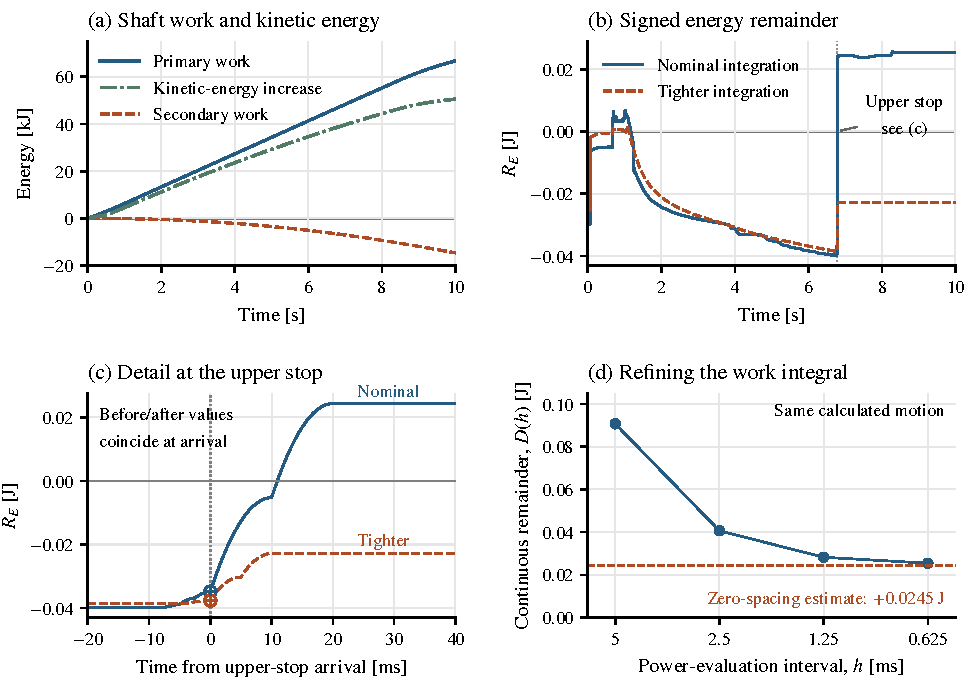
\includegraphics[width=\linewidth]{figures/results/verification/energy_balance.pdf}
  \caption{Energy accounting during the reference acceleration.
  (a) Nominal shaft work and kinetic-energy increase. Negative secondary
  work removes energy through the vehicle load; smaller terms are in
  \Cref{tab:verification_energy_ledger}.
  (b) Signed remainders for the nominal and tighter integrations.
  (c) Detail using each calculation's upper-stop arrival as time zero.
  Circles and crosses mark values immediately before and after arrest;
  each pair coincides. Lines do not bridge events.
  (d) Fixed nominal motion with successively halved maximum intervals
  between power evaluations. The dashed line estimates the zero-spacing
  remainder from the two finest intervals. Panels (b,c) use the finest
  interval, \SI{0.625}{ms}.}
  \label{fig:verification_energy_balance}
\end{figure}

Agreement at the kilojoule scale cannot by itself establish the accuracy of
this balance. Panel (b) shows the signed remainder: it stays below
\SI{0.040}{J} in magnitude at the sampled states in both integrations. The
nominal final value is \(+0.0254~\mathrm{J}\), or
\(4.88\times10^{-7}\) of the net work.

The apparently abrupt change near \SI{6.78}{s} needs closer examination
because it occurs near the upper-stop arrival. Arresting the shift motion
reduces stored kinetic energy. The capture loss must increase by the same
amount, leaving \(R_E\) unchanged at the instant of arrest; omitting that loss
would instead produce a jump in the remainder. Panel (c) enlarges this part
of panel (b), with the nominal and tighter calculations identified separately.
In each, the recorded values immediately before and after arrest coincide. The fast
change visible in panel (b) takes place over the adjoining continuous motion,
not across the instantaneous capture. The stop's energy removal is therefore
included without introducing a discontinuity in the balance.

Two refinements examine the small remainder. First, the calculated motion is
held fixed, but power is evaluated more frequently to improve the work and
sliding-loss integrals. Panel (d) shows the result as the maximum interval
between these evaluations is halved successively from \SI{5}{ms} to
\SI{0.625}{ms}. The summed continuous remainder falls from \SI{0.0907}{J}
to \SI{0.0254}{J}, with progressively smaller changes. The two finest
intervals give a zero-spacing estimate of \(+0.0245~\mathrm{J}\)
(\Cref{eq:energy_quadrature_extrapolate}). Finer integration of power therefore
reduces the discrepancy but does not appear to remove it. This estimate
concerns the work integrated along the calculated motion; it is not an error
bound on that motion.

Second, the motion itself is recomputed with tighter time-integration
settings. This changes the final remainder to \(-0.0228~\mathrm{J}\), while
leaving the final motion nearly unchanged: the shaft speeds change by less
than \SI{6.1e-5}{rad/s} and the belt speed by less than \SI{3.9e-6}{m/s}.
The small remainder is therefore sensitive to how the motion is calculated,
as well as to how power is integrated along it. Its final magnitude decreases
with each tested refinement, although these comparisons do not identify a
unique source of the remaining discrepancy. Signed work associated with
numerical drift during sticking is reported separately in \Cref{app:study_energy_consistency}; it is not
subtracted to improve this balance.

The energy account therefore holds to a small absolute remainder through
the acceleration, shifting and checked changes of constraint. Changes in the
retained kinetic and spring energy, together with the calculated sliding and
capture losses, account for the net shaft work over the complete transient,
including the instantaneous changes of velocity. The final energy balance
closes with remainder magnitudes of \(4.88\times10^{-7}\) and
\(4.38\times10^{-7}\) of the net shaft work in the nominal and tighter
integrations, respectively.
\FloatBarrier


\subsection{Solver Convergence}
\label{sec:results_solver_convergence}

The reliability of a transient calculation also depends on how accurately it
follows the motion in time. Satisfying the mechanical and energy balances
does not, by itself, establish that accuracy. The numerical check is
therefore whether the motion and its changes of contact and support approach
the same response as the integration is refined.

The full-throttle, level-ground acceleration provides a concrete example
of how the integration settings affect the calculated motion. It includes
primary engagement, low-ratio seating, free shifting and upper-stop arrival
within \SI{10}{s}.

\Cref{fig:verification_gross_hybrid_agreement} compares loose, intermediate
and tight integrations of this same case. The physical inputs and contact
rules remain fixed; only the integration controls change. Relative and
absolute tolerances control the solver's estimates of local error, while
the maximum step caps its adaptive integration step. The tight calculation
supplies the numerical reference.

The complete shift curves nearly coincide in panel (a). Panel (b) resolves
the difference: the loose integration gives shallower returns below the
engagement position and earlier seating, while the intermediate and tight
calculations agree closely on this motion. Below the engagement position,
the primary supplies no belt force or torque, so these differences change
when it carries belt load. Resolving the short contact changes therefore
requires more than agreement on the overall upshift.

\begin{figure}[!htb]
  \centering
  
\includegraphics[width=\linewidth]{figures/results/verification/gross_motion_hybrid_history.pdf}
  \caption{Three integrations of the same acceleration. The control triples
  $(\mathrm{rtol},\mathrm{atol},\Delta t_{\max})$ are approximately
  $(1.27\times10^{-2},1.27\times10^{-5},\SI{25.0}{ms})$ for the loose run,
  $(10^{-4},10^{-7},\SI{10}{ms})$ for the intermediate run and
  $(10^{-7},10^{-10},\SI{2.5}{ms})$ for the tight reference.
  In (b), negative displacement indicates primary separation. Markers identify
  low-ratio seating; the reference circle and intermediate cross nearly coincide.
  Curves retain separate continuous segments. Exact settings and the fixed
  numerical seating rule are documented in \Cref{app:study_solver_convergence}.}
  \label{fig:verification_gross_hybrid_agreement}
\end{figure}

\begin{samepage}
The complete response is therefore compared through all five state variables---the two shaft
speeds, belt speed, shift position and shift speed---together with the order
and timing of contact and support changes. When the same changes occur,
motion is compared at equal fractional progress between corresponding
events, keeping incoming and outgoing states separate. Otherwise, a small
timing offset could compare a velocity before capture with one already
changed by capture. Event times are checked separately on the actual clock,
so this alignment does not hide a timing difference.
\par\end{samepage}

To compare quantities with different units, each state difference is divided
by a fixed scale based on the reference motion. Their duration-weighted
root-mean-square (RMS) difference measures agreement over the complete
transient. Brief discrepancies can contribute little to this average, so
the largest sampled difference is also checked. These are differences from
a numerical reference, not an exact solution.

The wider refinement sweep combines eight relative tolerances with five
maximum-step caps, reducing absolute tolerance in proportion to relative
tolerance. The reference is tighter than every combination in this grid.
Shift speed supplies the largest scaled peak in every completed run;
panel (b) of
\Cref{fig:verification_solver_refinement} shows it in physical units.
Panel (c) shows the largest event-time difference. Both bands span the
completed step caps at each tolerance.

\begin{figure}[H]
  \centering
  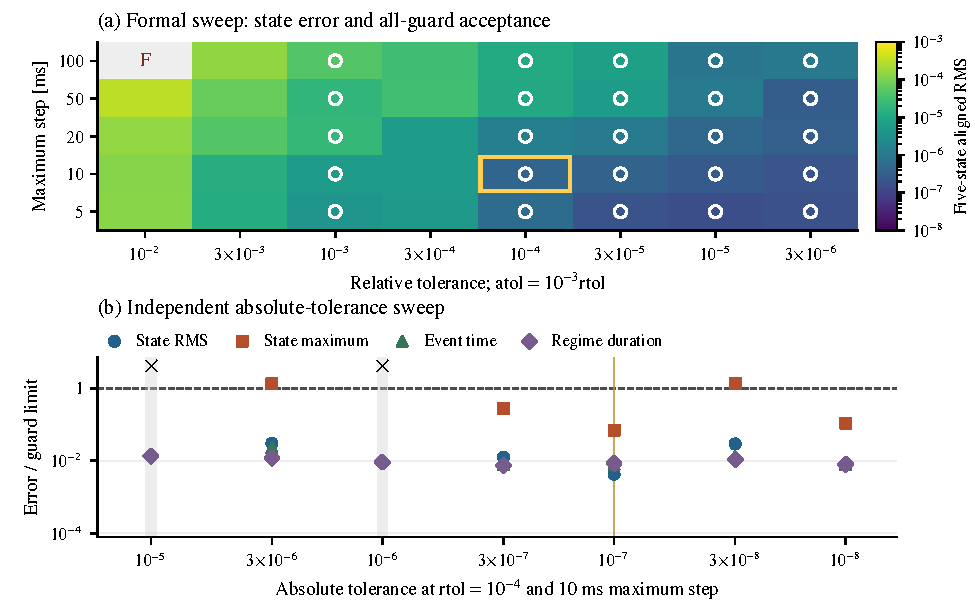
\includegraphics[width=\linewidth]{figures/results/verification/solver_refinement.pdf}
  \caption{State and timing differences from the tight numerical reference
  across the main refinement sweep. In (a), each cell is one tested
  tolerance/step-cap combination; F denotes the sole failed integration.
  Panels (b) and (c) span the minimum to maximum across the completed step
  caps at each tolerance: four at $10^{-2}$ and five elsewhere.
  The edges nearly coincide in (b). These bands describe variation between
  numerical settings, not statistical uncertainty. Lines connect tested
  tolerance levels; tighter tolerances lie to the right.}
  \label{fig:verification_solver_refinement}
\end{figure}

\begin{samepage}
The heatmap shows a substantial reduction in discrepancy as the controls
are tightened. Across the completed step caps, the largest RMS falls from
$3.23\times10^{-4}$ at $\mathrm{rtol}=10^{-2}$ to
$1.03\times10^{-6}$ at $3\times10^{-6}$. The local and timing measures
show that this improvement extends beyond the average motion. The peak
shift-speed difference falls from approximately \SI{22.4}{mm/s} to
\SI{0.00356}{mm/s}, while the largest event-time difference across caps
falls from \SI{7.93}{ms} to \SI{29.2}{\micro\second}.
Every completed main-grid calculation reproduces the reference order of
contact and support changes.
\par\end{samepage}

Only the coarsest combination, $\mathrm{rtol}=10^{-2}$ with a
\SI{100}{ms} cap, fails to complete and is marked F. At these loose settings,
a force evaluation would require the ramp to pull on the primary flyweight,
violating its one-sided contact condition. The finer integrations complete
without this failure, supporting its interpretation as a numerical failure
rather than a prediction of physical flyweight lift-off.

The bands also distinguish the roles of the two controls. At a given
tolerance, changing the step cap has little effect on the peak shift-speed
difference, but produces a wider spread in event-time differences. Both
controls therefore matter when assessing the complete transient, even
when one local measure has become insensitive to the step cap.

At the tightest main-grid tolerance, all five step caps give aligned
shift-position differences below \SI{0.068}{\micro\metre}, compared with
the approximately \SI{20}{mm} travel scale, and event-time differences below
\SI{30}{\micro\second}. Together with the reduction in the local speed
difference, this supports numerical convergence of the calculated
acceleration through engagement, shifting and stop arrival. Agreement
extends to the motion between changes of constraint and to when those
changes occur, under the fixed contact and seating rules.
\FloatBarrier

\subsection{Closure Conditioning and Root Structure}
\label{sec:results_closure_structure}

The time integration relies on a force and acceleration calculation at
each instant. Its reliability therefore also depends on whether the
mechanical balances remain solvable as the operating conditions change,
and whether the tractions required for sticking can be found consistently.

For a prescribed \((\lambda_p,\lambda_s)\),
\Cref{sec:engaged_mechanical_core} reduces these balances to a
\(6\times6\) linear system. Sliding supplies its traction directly from
kinetic friction; sticking uses this same system with trial tractions.
The implementation retains the two pulley torques among the unknowns,
as detailed in \Cref{app:num_fixed_lambda}. This gives an \(8\times8\)
system, but the mechanical solve remains the same: eliminating those
torques recovers the six-variable formulation.

First consider this \(8\times8\) system with the traction pair prescribed.
Four states are examined: low-ratio seating, mid-shift and upper-stop motion
from the level-ground acceleration, and a constructed opening state at
\(70\%\) engaged travel. At each state, the position, velocities and
applied shaft loads are held fixed while the traction pair is varied over
the static-friction range \([-0.65,0.65]^2\) and the wider
\([-2.6,2.6]^2\) diagnostic range.

The mechanical system has full rank at every sampled pair in both ranges,
so each trial gives a unique set of contact loads and accelerations.
\Cref{fig:verification_closure_robustness}(a) shows the condition number
of this \(8\times8\) system at the upper stop, after equilibration.
Its value at the operating pair is \(8.56\times10^3\), much lower than
the static-map maximum of \(1.05\times10^6\), indicating much less
numerical sensitivity there. The maximum lies among trials with negative
belt loading. Those linear systems still have a unique solution, but the
belt cannot sustain the calculated forces. Full rank and traction within
the static-friction range therefore do not replace the physical contact
checks.

\begin{samepage}
For sticking, a further question remains: which traction pair makes that
mechanical response preserve matching tangential accelerations of the belt
and pulley surfaces? Panel (b) shows these acceleration mismatches at the mid-shift state.
Each point still uses one fixed-traction mechanical solve; the solid and
dashed zero contours mark the pairs that preserve sticking at the primary
and secondary, respectively. Their intersection satisfies both conditions
and determines the sticking traction pair.
\par\end{samepage}

\begin{figure}[H]
  \centering
  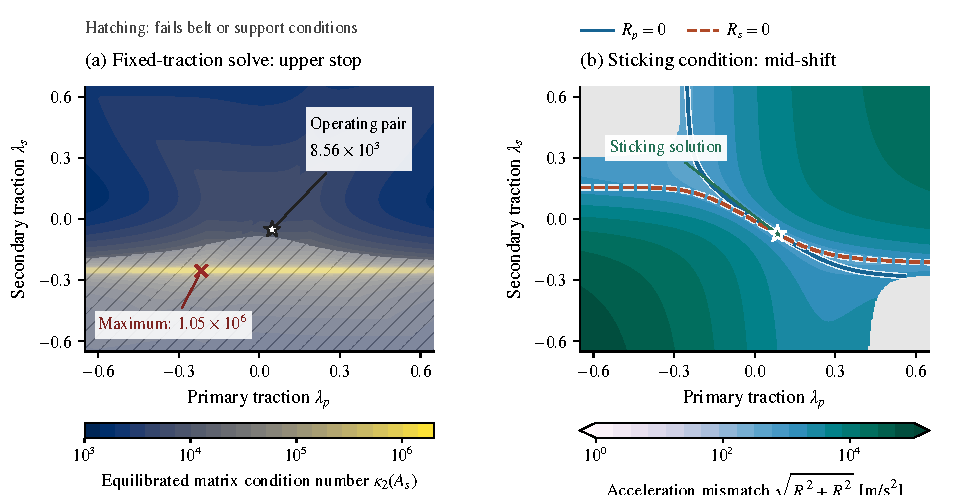
\includegraphics[width=\linewidth]{figures/results/verification/closure_robustness.pdf}
  \caption{The common mechanical solve and the additional sticking condition.
  Both panels use \(241\times241\) static-capacity grids.
  (a) Equilibrated mechanical condition number at the upper-stop state;
  hatching marks trials that fail belt-loading or support conditions.
  The cross is the sampled maximum and the star is the operating pair.
  (b) Dimensional acceleration mismatch at mid-shift, with
  \(R_j=a_{\mathrm{rel},j}\). The solid and dashed lines are the primary
  and secondary zero contours. Grey regions fail contact checks and are
  excluded from these contours.}
  \label{fig:verification_closure_robustness}
\end{figure}

Recovery of that intersection was checked from different starting guesses
at 15 operating states. Four come from the acceleration history; eleven
constructed cases cover forward and reverse rotation, low, middle and high
travel, increased shaft loading, and free opening and closing at three
travel positions. Their individual results are listed in
\Cref{tab:closure_named_states}.

At each state, seven starting values for each traction are combined into
49 starting pairs spanning the static-friction range. Repeating the search
from these different parts of the traction plane checks whether it returns
to the same solution. Of the 735 searches, 666 reach sticking, and every
accepted result at a given state recovers the same operating solution.

The remaining 69 attempts stop with nonzero acceleration mismatches.
Other starting guesses recover an admissible sticking solution at those
same states, so these failures concern finding an available root, rather
than insufficient friction to sustain sticking. A wider starting grid at
the four mapped states also recovers only their existing solutions.
The same sticking response is therefore recovered repeatedly at each
state, although the numerical search remains sensitive to its starting guess.

The applied shaft torques also affect the acceleration mismatches. To
examine how the sticking solution changes with loading, a constructed
opening state is held at \(95\%\) engaged travel, \(-40~\mathrm{mm/s}\)
shift speed and \(3000~\mathrm{rpm}\) primary speed. The primary boundary
torque is fixed at \(-81.15~\mathrm{N\,m}\) while the secondary torque
varies. Both shafts rotate positively, so at the selected positive secondary
torque the secondary supplies power and the primary absorbs it. These are
fixed-state bench loads, rather than another vehicle trajectory.

At \(+189.96~\mathrm{N\,m}\) secondary torque,
\Cref{fig:verification_closure_fold}(a) has two intersections. Both pairs
satisfy sticking and pass the friction, belt-loading and actuator-contact
checks. They give different responses: the secondary normal resultant is
\SI{2.401}{kN} at root 1 and \SI{1.669}{kN} at root 2, with different
accelerations as well. Root 2 is closer to loss of wrap contact: its minimum
secondary local normal loading is \SI{0.243}{N/rad}, compared with
\SI{20.84}{N/rad} at root 1.

Panel (b) shows how both pairs belong to one connected sticking branch.
As secondary traction increases, the required secondary torque first rises
and then falls, turning near \SI{197.39}{N.m}. The selected load consequently
intersects both sides of the turn. Increasing traction changes the normal
loads and accelerations through the coupled balances, so it need not increase
the compatible boundary torque monotonically. The mechanical matrix remains
full rank throughout this branch: each prescribed pair still gives one
force response, while two different pairs can satisfy the sticking conditions
under the same applied load.

\begin{figure}[H]
  \centering
  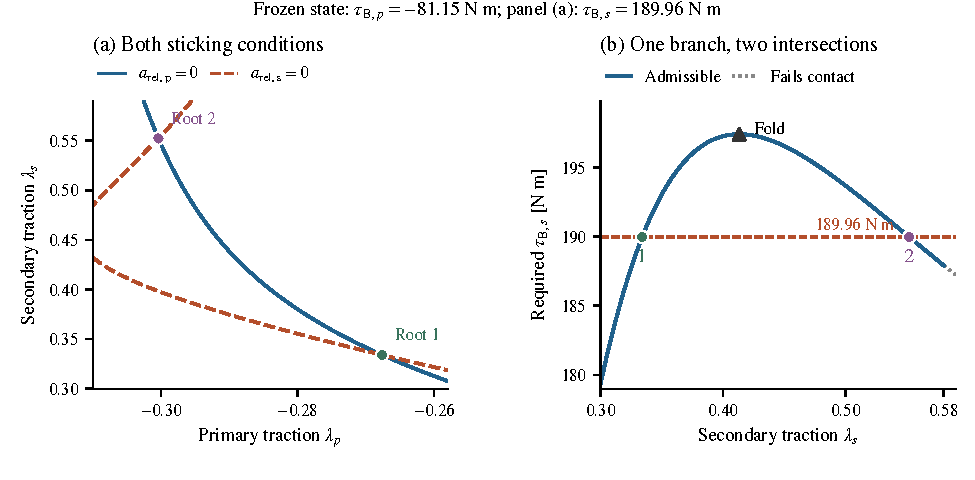
\includegraphics[width=\linewidth]{figures/results/verification/sticking_closure_fold.pdf}
  \caption{Two sticking responses at the same opening state and applied load.
  (a) Dimensional acceleration mismatch and the two zero contours at the
  selected shaft torques. The marked roots use the same identifiers in both
  panels; grey marks loss of local wrap compression.
  (b) Secondary boundary torque required to maintain sticking along the
  connected branch, with primary boundary torque fixed. The selected load
  intersects the branch twice. The dotted extension fails local wrap
  compression and is not an admissible continuation. Secondary traction is
  a branch coordinate, not time or shift position. Exact state, loads and
  signed responses are given in \Cref{app:study_closure_conditioning}.}
  \label{fig:verification_closure_fold}
\end{figure}

This distinction also matters when only one contact sticks. The targeted
example in \Cref{app:study_closure_conditioning} admits two secondary sticking
tractions with primary traction fixed at its kinetic value, at the onset of
primary sliding. Reducing the search to one unknown therefore does not by
itself ensure a unique sticking solution.

\begin{samepage}
Within the sampled static and expanded ranges, the mechanical solve remains
robust, while the operating-state searches repeatedly recover a single
sticking root. The selected alternatives are locally unique away from the
fold. Using the preceding accepted traction pair helps CINDER follow the
nearby branch and avoid root jumps, while rechecking compatibility and
contact limits. This guides the numerical choice without establishing a
physical selection law. No root jump or effect of an alternative root was
detected in the other reported calculations.
\par\end{samepage}
\FloatBarrier

\begingroup
\clubpenalty=10000
\widowpenalty=10000
\displaywidowpenalty=10000

\providecommand{\CINDERResultsFigure}[4][44mm]{%
  \IfFileExists{#2}{%
    \includegraphics[width=\linewidth,height=0.56\textheight,keepaspectratio]{#2}%
  }{%
    \fbox{%
      \begin{minipage}[c][#1][c]{\dimexpr\linewidth-2\fboxsep-2\fboxrule\relax}
        \centering\small
        \textbf{#3}\par\medskip
        #4\par\medskip
        \footnotesize\nolinkurl{#2}
      \end{minipage}%
    }%
  }%
}
\providecommand{\CINDERResultsDraftNote}[2]{%
  \begin{tcolorbox}[title={Evidence to complete: #1},fonttitle=\bfseries]
    \small #2
  \end{tcolorbox}%
}

% ==============================================================
\section{Independent Transient-Model Benchmark}
\label{sec:results_ballew_benchmark}

The preceding checks establish the consistency of CINDER's calculated motion.
A comparison with an independent formulation can now examine how that motion
changes when the belt is described in more detail. Ballew's discretized
rubber-belt model provides a five-second ATV acceleration case with published
shaft-speed histories, primary clamping force and controller gains
\citep{Ballew2015}. Its speeds are produced under feedback, however, so the
comparison must consider both the motion and the force used to obtain it.
Reconstructing the feedback allows the controller to adjust CINDER's clamp
demand; imposing Ballew's published force instead tests the response to a
common force history.

\subsection{Benchmark Reconstruction}
\label{sec:results_ballew_reconstruction}

Both protocols use the same reconstructed belt geometry, shaft inertias and
ATV road-load boundary, with a constant primary torque of \SI{18}{N.m} and
secondary closing force of \SI{2000}{N}. The initial shaft speeds are Ballew's
tabulated \(2500\) and \(1136~\mathrm{rpm}\); a compatible belt speed and shift
position follow from the reconstructed geometry. These inputs belong to the
published benchmark rather than the Baja reference. \Cref{app:study_ballew}
gives the source quantities, their translation into CINDER and the numerical
settings. The accompanying
\ResultsCode{studies/ballew-2015/provenance/RECONSTRUCTION.md}{reconstruction record}
identifies the source locations, digitization procedure and choices needed to
re-create the case. No physical parameter or controller gain is fitted to the
reference histories.

The translations preserve the published belt mass and combined shaft
inertias. Friction coefficients are converted between the two normal-force
conventions so that the same clamp gives the same gross tangential capacity.
Both literal moving-sheave masses are set to zero because Ballew obtains
radial position from an algebraic axial-force balance. CINDER's belt inertia
and reduced shift dynamics remain active. Ballew also initializes internal
belt-deformation states, including zero longitudinal tension, that have no
direct counterpart in CINDER. The reconstruction therefore matches the
specified external conditions without making the internal initial states
identical.

\subsection{Closed- and Open-Loop Comparisons}
\label{sec:results_ballew_closed_loop}
\label{sec:results_ballew_force_replay}

In the closed-loop protocol, the primary clamp regulates speed toward
\(2500~\mathrm{rpm}\). Ballew reports the PI and feed-forward gains but does
not fully specify the controller equation. The reconstruction uses those
gains in the force law of \Cref{eq:ballew_pi_force_law}, with zero initial
integral error and no added saturation. The published force is an output
reference for this comparison.

The open-loop protocol instead prescribes that force. Ballew's digitized
Figure~45 history is applied by piecewise-linear interpolation, with its first
visible value held back to \(t=0\). All other reconstructed inputs are
unchanged. The two columns of \Cref{fig:results_ballew_protocols} therefore
compare the same shaft quantities while distinguishing a force calculated
by feedback from one supplied as an input.

\begin{figure}[H]
  \centering
  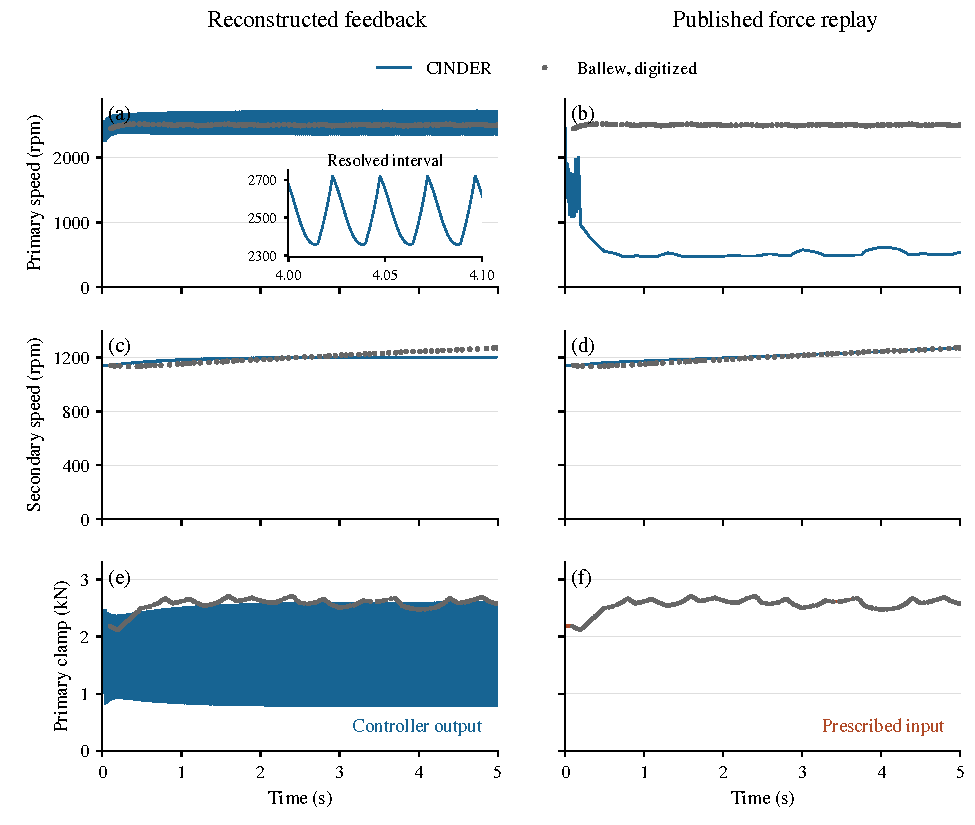
\includegraphics[width=\linewidth]{figures/results/ballew/protocol_comparison.pdf}
  \caption{Reconstructed feedback and prescribed-force replay against Ballew's
  simulated histories. Corresponding panels use the same scales. Points are
  digitized from Figures~41 and~45 \citep{Ballew2015}; the CINDER traces are
  unsmoothed, and the inset resolves the primary-speed oscillation over
  \SI{0.1}{s}. The primary force is a controller output in (e) and a prescribed
  input in (f). Both protocols share the secondary clamp and shaft boundaries.}
  \label{fig:results_ballew_protocols}
\end{figure}

With feedback, the primary speed remains near the target but oscillates much
more strongly than the published history. The secondary speed also differs
in shape: CINDER levels off near \(1200~\mathrm{rpm}\), while Ballew's result
continues toward \(1270~\mathrm{rpm}\). Their speed RMSE values are
\(110\) and \(33~\mathrm{rpm}\), respectively
(\Cref{tab:results_ballew_comparison}). The primary-clamp RMSE is much larger
relative to its reference, at \SI{1.20}{kN}, or \(46.66\%\).
Thus the modest shaft-speed errors coexist with a substantially different
force demand. Because clamping governs both the shift balance and available
traction, that difference matters to the transmission response.

\begin{table}[H]
  \centering\small
  \begin{tabular}{@{}lrr@{}}
    \toprule
    Quantity & Closed loop & Force replay \\
    \midrule
    Primary speed & \(110~\mathrm{rpm}\;(4.42\%)\) & \(1946~\mathrm{rpm}\;(77.89\%)\) \\
    Secondary speed & \(32.6~\mathrm{rpm}\;(2.71\%)\) & \(13.1~\mathrm{rpm}\;(1.09\%)\) \\
    Shaft-speed ratio & \(0.100\;(4.81\%)\) & \(1.633\;(78.31\%)\) \\
    Primary clamp & \(1196~\mathrm{N}\;(46.66\%)\) & Prescribed input \\
    \bottomrule
  \end{tabular}
  \caption{RMSE against the digitized reference histories. Parentheses give
  RMSE as a percentage of the mean absolute reference value at the comparison
  samples. The shaft-speed ratio is \(\omega_p/\omega_s\). Speeds and force
  are compared at their native digitization times; the ratio uses the union of
  the two speed grids over their common interval. The initial force hold used
  for replay is excluded from the closed-loop force comparison.}
  \label{tab:results_ballew_comparison}
\end{table}

Removing the controller's adjustment makes the primary-speed discrepancy much
larger. Under force replay, CINDER's primary speed falls to roughly
\(500~\mathrm{rpm}\) after the initial transient, rather than remaining near
\(2500~\mathrm{rpm}\). Its primary-speed and shaft-ratio errors approach
\(78\%\), even though the secondary speed is closer to Ballew's result than
in the controlled case. Agreement at the output shaft alone would therefore
conceal a very different relation between the two shaft motions.

\subsection{Internal Motion and Slip}
\label{sec:results_ballew_internal_motion}

The controlled case also illustrates why similar shaft speeds need not imply
similar belt motion. This benchmark has no relative sheave-rotation mechanism,
so \(\omega_p/\omega_s\) would equal
\(r_{s,\mathrm{eff}}/r_{p,\mathrm{eff}}\) if both contacts rolled without slip.
\Cref{fig:results_ballew_internal_response}(a,b) compares these ratios within
CINDER. The shaft-speed ratio stays near two, while the radius ratio repeatedly
moves between approximately \(0.46\) and \(2.49\), reaching the low-ratio seat.
The difference between them shows that the shaft speeds do not track the
large excursions of the belt along the pulleys. Slip accommodates that
relative motion and dissipates energy. Panel~(c) shows \SI{19.7}{kJ} of
cumulative modeled slip loss over the five seconds, contributed by both
contacts. These internal quantities describe CINDER's response; corresponding
histories are not available from the published benchmark for comparison.

\begin{figure}[H]
  \centering
  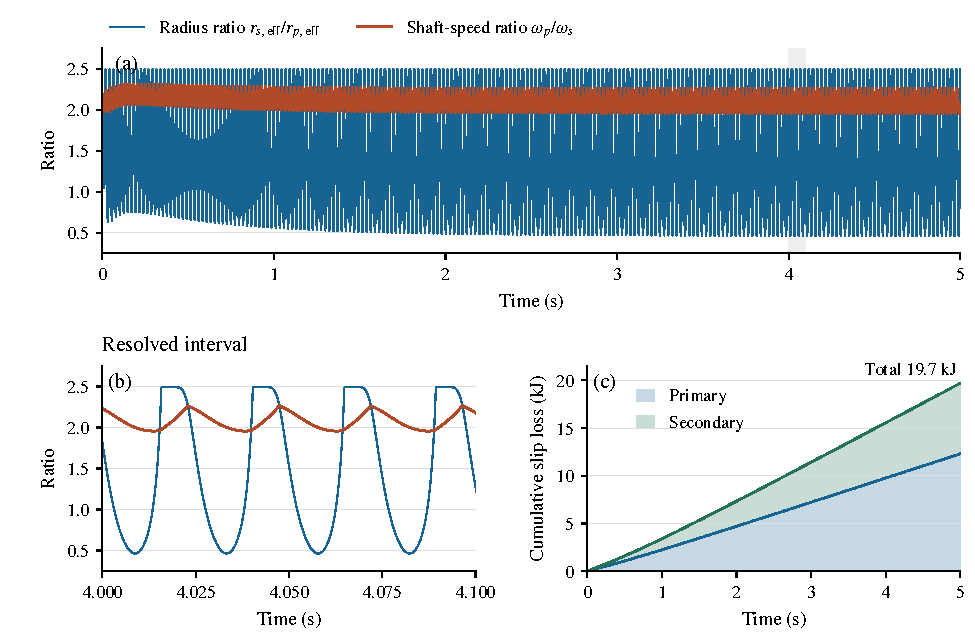
\includegraphics[width=\linewidth]{figures/results/ballew/internal_response.pdf}
  \caption{Internal response under reconstructed feedback. (a) Shaft-speed
  and effective-radius ratios over the complete run. The shaded interval is
  expanded in (b), showing the actual motion rather than an averaged ratio.
  (c) Stacked cumulative slip losses at the primary and secondary contacts;
  the upper boundary is their sum. Continuous segments retain their separate
  event endpoints.}
  \label{fig:results_ballew_internal_response}
\end{figure}

Because the oscillations occur over a short timescale, their numerical convergence was checked. Reducing the
maximum step from \SI{1}{ms} to \SI{0.5}{ms} and \SI{0.25}{ms}, and tightening
both integration tolerances at the \SI{0.5}{ms} limit, leaves these
oscillations essentially unchanged. Across the three refinements, the largest
same-time RMS differences from the nominal run are only
\(0.032~\mathrm{rpm}\) in primary speed and \SI{0.160}{N} in clamp force.
The sticking/sliding and support changes also retain their order, although
the number of recorded slip-direction updates differs.
\Cref{app:ballew_numerics} gives the refinement results and event comparison.
The benchmark discrepancy therefore persists under these changes in numerical
resolution.

\subsection{Interpretation of the Model-Form Difference}
\label{sec:results_ballew_interpretation}

Force replay shows that the discrepancy does not arise solely from the
reconstructed controller: the models also respond differently when its
adjustment is removed. The principal difference in the belt descriptions is
the motion each can represent. Ballew resolves internal deformation and local nodal motion,
whereas CINDER uses a fixed belt length, one transport speed and a prescribed
path controlled by the shift coordinate. Local deformation and force
redistribution can therefore alter the response to a given clamp. The
unmatched initial tension and other necessary reconstruction choices still
limit how directly this difference can be assigned to any one belt mechanism.

\begin{samepage}
Compliance and damping have different roles in that explanation. Compliance
allows energy storage and redistribution of motion; damping removes energy.
Figures~41 and~45 are Ballew's case without the added linear inter-node damper,
although the source model retains angular damping. The mismatch cannot be
attributed to the added linear damper used in his separate comparison
\citep[Figures~40--45]{Ballew2015}. Isolating the remaining causes would require
controlled changes to the belt descriptions.
\end{samepage}

Taken together, the two protocols show that matching a controlled speed is an
incomplete test of a CVT model. The required clamp and the response when that
clamp is imposed provide additional, distinct information. Here they reveal
a substantial difference in the reconstructed relation between clamp force,
shift and slip, despite the closer controlled shaft histories. The benchmark
therefore identifies where CINDER's reduced belt description needs further
physical assessment; it is an independent model comparison, not experimental
validation of either formulation.
\FloatBarrier

\section{Dynamic Mechanics Retained by CINDER}
\label{sec:results_dynamic_mechanics}

At a given mechanism position, the same centrifugal or torque loading need
not produce the same clamp during a transient. Part of that loading may be
required to accelerate the actuator itself. A quasi-static actuator law omits
that inertial demand. The resulting approximation may reproduce a
smooth response while changing the reaction to a rapid load disturbance.
The relevant question is therefore which retained inertial contributions are
actually excited, and when their omission changes the solved CVT motion.

The comparisons begin with the primary and secondary mechanisms under this
common question, then examine the transient terms retained in the reduced
belt. The actuator variants use the interchangeable interface in
\Cref{app:num_affine_assembly}; their exact reductions and redistribution of
rotating inertia are given in \Cref{app:results_quasistatic_actuators}.
Evaluating an omitted term on the full-model trajectory isolates its local
contribution. Integrating the corresponding reduced model answers the
different question of whether that omission changes the trajectory itself.

\subsection{Primary Actuation Dynamics}
\label{sec:results_primary_actuator_dynamics}

\subsubsection{Centrifugal drive and the motion it must accelerate}
\label{sec:results_primary_dynamic_terms}

The flyweights both generate the centrifugal closing action and move about
their pivots as the primary sheave shifts. These roles involve different
inertias. The shaft-axis map \(J_{f,p}(x_p)\) sets the centrifugal drive,
whereas the pivot inertia \(I_f\) sets the torque required to accelerate the
flyweight motion. Writing \Cref{eq:primary_flyweight_axial_force} as its
quasi-static part plus its omitted contribution gives
\begin{equation}
\begin{aligned}
 F_{\mathrm{fw},x_p}
 &=F_{\mathrm{fw},x_p}^{\mathrm{QS}}+\Delta F_{\mathrm{fw},x_p},\\
 F_{\mathrm{fw},x_p}^{\mathrm{QS}}
 &=\frac12\omega_p^2\frac{dJ_{f,p}}{dx_p},\\
 \Delta F_{\mathrm{fw},x_p}
 &=-I_f\left(\frac{dq_f}{dx_p}\right)^2\ddot x_p
   -I_f\frac{dq_f}{dx_p}\frac{d^2q_f}{dx_p^2}\dot x_p^2.
\end{aligned}
\label{eq:results_primary_dynamic_decomposition}
\end{equation}

The acceleration term has a positive inertial coefficient
\begin{equation}
 m_{f,\mathrm{ref}}
 =I_f\left(\frac{dq_f}{ds}\right)^2,
 \label{eq:results_flyweight_reflected_inertia}
\end{equation}
because \(x_p=s\). Thus even a modest pivot inertia can resist shifting
strongly if the mechanism requires a large flyweight rotation per unit sheave
travel. The final term in
\Cref{eq:results_primary_dynamic_decomposition} instead depends on how that
motion ratio changes along the ramp. A large centrifugal force alone does not
determine either correction.

This distinction gives a useful first sensitivity test before selecting a
transient. For a sheave excursion of fixed shape and amplitude executed over
a time scale \(T\), both \(\ddot x_p\) and \(\dot x_p^2\) scale as
\(T^{-2}\). Shortening the same prescribed excursion can therefore magnify
the dynamic correction without changing the centrifugal force at the same
position and shaft speed. This is a kinematic scaling argument; in an actual
CVT the excursion and its duration are themselves outcomes of the coupled
solve.

% NEW DISPLAY FROM EXISTING FORMULATION / ARCHIVED PRIMARY STUDY.
% Show q'_f and I_f(q'_f)^2 over admissible travel, then signed axial
% corrections and the separate shaft-angular-momentum terms on selected
% reference/rapid-load traces. The primary numerical archive must be recovered.
\begin{figure}[tbp]
  \centering
  \CINDERResultsFigure[54mm]
    {figures/results/dynamics/primary_geometry_and_response.pdf}
    {New figure: primary geometry, excitation, and response}
    {Map the motion-ratio-weighted pivot inertia over travel. Below it, show
     signed centrifugal/inertial force terms and a matched full-versus-QS
     primary comparison. Keep the shaft-torque correction separate from the
     axial-force correction. Quantitative primary evidence is pending.}
  \caption{Primary-actuator comparison to be assembled from the fixed-pivot
  mechanism map and its matched dynamic and quasi-static runs. The upper
  display locates geometric sensitivity; the lower displays test whether the
  realized motion excites that sensitivity and changes shaft or shift
  response. All variants use the same tested primary mechanism and the
  inertia treatment in \Cref{app:results_quasistatic_actuators}.}
  \label{fig:results_primary_dynamics}
\end{figure}

\subsubsection{Small force corrections do not make flyweight inertia irrelevant}
\label{sec:results_primary_scope}

The reference actuator study identifies ordinary continuous Baja operation as
close to quasi-static. A small primary correction means that little of the
centrifugal action is consumed by accelerating the flyweights about their
pivots. The comparison in \Cref{fig:results_primary_dynamics} separates this
force-level statement from its consequence for shaft and shift motion.
A local measure is
\begin{equation}
 \Pi_p(t)=
 \frac{|\Delta F_{\mathrm{fw},x_p}(t)|}
      {|F_{\mathrm{fw},x_p}^{\mathrm{QS}}(t)|},
 \qquad F_{\mathrm{fw},x_p}^{\mathrm{QS}}\ne0.
 \label{eq:results_primary_dynamic_number}
\end{equation}
The signed force terms must accompany this ratio so that a small denominator
or cancellation between corrections is not mistaken for a large change in
physical loading.

\CINDERResultsDraftNote{P1 --- recover the primary comparison}{
  The supplied commercial-actuator recap gives the qualitative ordinary-Baja
  conclusion, but not the primary's force peaks, shaft-torque corrections, or
  paired trajectory errors. Insert those from the archived fixed-pivot study.
  Use at least the smooth reference interval and the strongest admissible
  primary transient already tested; report the interval, denominator, and
  full/QS comparison. If those outputs do not support the qualitative
  statement for the primary separately, revise that statement. No numerical
  primary bound or universal negligible-inertia claim is assumed.}

There is a second distinction to preserve. The same flyweight mass also
changes the primary's shaft-axis angular momentum. Its contribution to the
rotational balance is
\begin{equation}
 \frac{d}{dt}\!\left[J_{f,p}(s)\omega_p\right]
 =J_{f,p}(s)\dot\omega_p
  +\frac{dJ_{f,p}}{ds}\dot s\,\omega_p.
 \label{eq:results_primary_angular_momentum_terms}
\end{equation}
Even when the pivot-acceleration force is small, outward flyweight motion
changes the rotating inertia. During upshift, angular momentum is required
to move that mass outward; during backshift, the redistribution reverses.
The axial-force comparison and the shaft-torque comparison therefore answer
different questions. In particular, the trajectory ablation changes the
mechanism's inertial coupling as specified in the appendix; it is not a test
of deleting a single axial term while everything else remains identical.

The primary result is consequently specific to the fixed-pivot roller
mechanism examined here. It can justify the quasi-static force approximation
for that mechanism over the supported operating intervals, while the maps in
\Cref{eq:results_primary_dynamic_decomposition} identify what must be checked
for another design. Neither greater flyweight mass nor a similar static
clamp curve, by itself, establishes the size of the dynamic error.

\subsection{Secondary Helix Dynamics and Transient Sensitivity}
\label{sec:results_secondary_helix}

\subsubsection{The helix converts rotational inertia into axial response}
\label{sec:results_secondary_dynamic_terms}

The secondary adds a direct route by which shaft acceleration changes clamp.
Its movable assembly rotates with the shaft and relative to it through the
helix. The torque available for axial reaction must therefore supply both
motions. Define the quasi-static reacted torque, with the formulation's
symmetric face share, as
\begin{equation}
 \tau_{s,\mathrm{helix}}^{\mathrm{QS}}
 =\frac{\tau_s}{2}
  +k_{s,\theta}\bigl(\theta_{s,\mathrm{pre}}-\theta_s\bigr).
 \label{eq:results_secondary_qs_torque_recalled}
\end{equation}
Then \Cref{eq:secondary_helix_closing_force} separates into
\begin{equation}
\begin{aligned}
 F_{\mathrm{helix},x_s}
 &=\frac{d\theta_s}{dx_s}\,
   \tau_{s,\mathrm{helix}}^{\mathrm{QS}}
   +\Delta F_{\mathrm{helix},x_s},\\
 \Delta F_{\mathrm{helix},x_s}
 &=-I_{s,M}\frac{d\theta_s}{dx_s}\dot\omega_s
   -I_{s,M}\left(\frac{d\theta_s}{dx_s}\right)^2\ddot x_s\\
 &\quad-I_{s,M}\frac{d\theta_s}{dx_s}
                 \frac{d^2\theta_s}{dx_s^2}\dot x_s^2.
\end{aligned}
\label{eq:results_secondary_dynamic_decomposition}
\end{equation}

The three omitted contributions are driven by shaft acceleration, axial
acceleration, and changing helix motion ratio. The first can remain active
even while the sheave is instantaneously stationary. The second changes the
inertia multiplying axial acceleration in
\Cref{eq:completed_secondary_axial_balance}. Its contribution to the shared
shift coordinate is
\begin{equation}
 m_{h,\mathrm{ref}}
 =I_{s,M}\left(\frac{d\theta_s}{ds}\right)^2.
 \label{eq:results_helix_reflected_inertia}
\end{equation}
The force correction and the reflected inertia are thus two appearances of
the same mechanism, not separate effects that can be assessed independently
once the trajectory changes.

The equation also distinguishes excitation time scales. A change in shaft
speed over a shorter interval increases the first term through
\(\dot\omega_s\); a fixed-shape axial excursion executed more rapidly
increases the acceleration and squared-velocity contributions. A constant-angle
helix removes the local profile-curvature term, but retains both acceleration
terms. Nonlinear mapping from \(x_s\) to \(s\) may still introduce
\(\dot s^2\) contributions in the shared-coordinate equations.

Geometry can amplify these contributions strongly because the motion ratio
appears squared in the reflected axial inertia. The commercial-secondary
estimate in \Cref{fig:results_secondary_scaling} illustrates why physical
rotational inertia and motion ratio must be considered together. Its motion
ratio is weaker than the Baja reference, yet the larger movable-member inertia
raises the nominal reflected local axial inertia to approximately
\(1.49\) times the reference at \(31^\circ\). The low and high estimates
span approximately \(0.45\) to \(2.92\) times the reference. The
\(28^\circ\) high-estimate sensitivity reaches approximately \(3.72\).
These are component estimates, not measurements of a complete commercial CVT
response.

% SOURCE: commercial-actuator recap pp. 2, 5--6.
% NEW COMPOSITION: show I*H^2 contours or curves, the Baja point, and low/
% nominal/high hardware estimates. A demand panel may use prescribed
% accelerations, but must label these as sensitivity inputs, not trajectories.
\begin{figure}[tbp]
  \centering
  \CINDERResultsFigure[48mm]
    {figures/results/dynamics/secondary_inertia_scaling.pdf}
    {Existing estimates + new equation-based display}
    {Compare movable rotational inertia, helix motion ratio, and their squared
     product. Mark Baja and the low/nominal/high commercial estimates; separate
     component-level prescribed acceleration sensitivity from simulated motion.}
  \caption{Secondary-actuator sensitivity to movable-member inertia and helix
  geometry. The coefficient \(I_{s,M}(d\theta_s/dx_s)^2\) is local axial
  reflected inertia; conversion to the shared shift coordinate also includes
  \((dx_s/ds)^2\). The provisional commercial estimates show that a less
  aggressive motion ratio need not imply a smaller dynamic contribution.}
  \label{fig:results_secondary_scaling}
\end{figure}

\subsubsection{A continuous transient with a measurable response change}
\label{sec:results_secondary_continuous}

To connect that scaling to motion, the nominal commercial helix geometry and
movable-member rotational inertia are inserted into the otherwise reference
Baja system. A secondary torque increment of \(-120~\mathrm{N\,m}\) is
applied over \(25~\mathrm{ms}\) from a conditioned state near the middle of
active shift. The selected case remains in clean continuous operation and
compares the full helix with its quasi-static counterpart. The unchanged host
makes this a mechanism-transplant experiment, not a reconstructed prediction
for a Sidewinder vehicle.

The total relative helix-reaction correction is evaluated on the full-model
trajectory as
\begin{equation}
 \Pi_{s,\mathrm{total}}(t)
 =\frac{I_{s,M}|\dot\omega_s+\ddot\theta_s|}
        {|\tau_{s,\mathrm{helix}}^{\mathrm{QS}}|},
 \qquad \tau_{s,\mathrm{helix}}^{\mathrm{QS}}\ne0.
 \label{eq:results_secondary_dynamic_number}
\end{equation}
It reaches \(7.87\%\) in the nominal case, with an approximately
\(89.3~\mathrm{N}\) peak dynamic helix-force correction. The quasi-static
torque magnitude remains above \(92.2\%\) of its onset value, so the peak
relative correction is not generated by a denominator approaching zero.
The shaft-acceleration term dominates this example. The component maxima are
not added to obtain the total: the signed contributions are combined at each
instant before their magnitude is taken.

A local correction is not yet a trajectory error. Each model is therefore
also run with a zero-disturbance control. For any output \(y\), the compared
perturbation responses are
\begin{equation}
 \delta y^{M}(t)=y^{M}_{\mathrm{loaded}}(t)-y^{M}_{\mathrm{control}}(t),
 \qquad M\in\{\mathrm{full},\mathrm{QS}\}.
 \label{eq:results_actuator_perturbation_response}
\end{equation}
\Cref{fig:results_secondary_continuous_response} compares these responses
alongside the actual stressed trajectories. In the nominal case,
\(\max|\delta y^{\mathrm{full}}-\delta y^{\mathrm{QS}}|\) is
\(0.274~\mathrm{mm}\) for shift, \(40.4~\mathrm{rpm}\) for primary speed,
and \(109.1~\mathrm{N}\) for secondary clamp. Under the same disturbance,
the high estimate reaches a \(13.6\%\) reaction correction and a
\(68.5~\mathrm{rpm}\) primary-speed response difference.

% SOURCE: commercial-actuator recap pp. 3--4, 7--12.
% CASE: S_s50_m120_r25ms, nominal 31-degree estimate; low/high repeat same
% forcing. Include each model's unforced control in response extraction.
\begin{figure}[tbp]
  \centering
  \CINDERResultsFigure[57mm]
    {figures/results/dynamics/secondary_continuous_response.pdf}
    {Existing results: continuous secondary response}
    {Show signed dynamic contributions and quasi-static torque, then actual
     stressed motion and full/QS perturbation-response differences. Include
     the low/nominal/high sensitivity without mixing unlike response units.}
  \caption{Continuous-transient consequence of the commercial-secondary
  mechanism transplant. The nominal case uses a \(-120~\mathrm{N\,m}\)
  added secondary torque over \(25~\mathrm{ms}\). Force diagnostics are
  evaluated on the full-model motion. Perturbation-response differences
  subtract each model's own zero-disturbance control as defined in
  \Cref{eq:results_actuator_perturbation_response}; they are not raw differences
  between independently conditioned trajectories.}
  \label{fig:results_secondary_continuous_response}
\end{figure}

This example establishes a secondary dynamic effect without relying on a
contact loss or an almost-vanishing static reaction. The gross trajectories
remain close, but the disturbance-induced response changes measurably. The
low, nominal, and high hardware estimates provide a sensitivity range; they
are not statistical confidence bounds on a measured machine.

\subsubsection{Rapid backshift couples reaction, inertia, and traction}
\label{sec:results_secondary_hybrid_response}

A more sensitive response occurs when the transient approaches a traction
transition. The severe reversal case uses the reference secondary with
\(270^\circ\) torsional preload and a conditioned state near \(30\%\)
active shift. Primary applied torque is blended toward
\(-28~\mathrm{N\,m}\) over \(50~\mathrm{ms}\). The full and quasi-static
helix systems receive the same initial state and external disturbance.
Both use the zero-clearance bilateral slot, so the comparison changes the
movable-member dynamics rather than permitting detachment in only one model.

\Cref{fig:results_secondary_sensitive_transient} shows that the trajectories
remain close until the late contact event, after which the quasi-static
model backshifts more rapidly. It leaves stick approximately
\(4.66~\mathrm{ms}\) earlier and accumulates approximately
\(4.66~\mathrm{ms}\) more non-stick duration within the reported window.
The maximum shift separation is \(2.026~\mathrm{mm}\). Near the event,
\(I_{s,M}(d\theta_s/ds)^2\) contributes approximately \(7.48~\mathrm{kg}\)
to the full model's shift-inertia accounting. This is a reflected coefficient,
not additional physical mass attached to the sheave.

The reduced model returns the movable rotational inertia to rigid shaft
rotation. It consequently retains that rotating hardware but loses its
resistance to relative helix motion. The resulting shift acceleration feeds
back into the reaction terms in
\Cref{eq:results_secondary_dynamic_decomposition}, changing the clamp and
traction solution. This explains why the difference is not captured by
subtracting an inertial force from a fixed quasi-static trajectory. The
trajectory changes as well. The extra resistance to rapid backshift is
inertial; it is not an added dissipative damper.

% SOURCE: helix checkpoint pp. 6--10.
% CASES: E58_reversal_270_s30_engine_m28_r050 and
% E58_stock_300_s30_output_m120_r002, with E5.7 parent chronology.
% REQUIRED NEW COMPOSITION: common absolute event time; shift, signed helix
% terms, normal load, and contact strips. Show stock contrast separately.
% Avoid labelling the archived ratio field as omega_s/omega_p: see S1.
\begin{figure}[tbp]
  \centering
  \CINDERResultsFigure[60mm]
    {figures/results/dynamics/secondary_sensitive_transient.pdf}
    {Existing results: severe transient and high-margin contrast}
    {Severe pair: shift response, reflected inertia, helix reaction, and exact
     contact histories through the event. Adjacent contrast: the stock
     high-margin case on explicitly stated axes. Preserve absolute event-time
     differences rather than aligning away the change being measured.}
  \caption{Secondary-helix dynamics near a sensitive traction event, contrasted
  with a high-margin stock case. In the severe case, full and quasi-static
  models start from the same conditioned state under the same forcing.
  The stock contrast uses \(300^\circ\) preload and a different disturbance,
  an added secondary torque of \(-120~\mathrm{N\,m}\) over
  \(2~\mathrm{ms}\); it is not a preload-only comparison. Contact histories
  and shift motion are displayed with their original timing.}
  \label{fig:results_secondary_sensitive_transient}
\end{figure}

The reaction chronology adds an important distinction. In the selected
full-dynamic reversal, the quasi-static reacted torque is still approximately
\(+1.811~\mathrm{N\,m}\) when the dynamic correction cancels it. The
required slot reaction then changes sign. Yet secondary normal load remains
positive: across the thirty crossing cases in the chronology analysis, the
smallest reported secondary resultant at a helix crossing is approximately
\(827~\mathrm{N}\). Those crossings did not coincide with loss of the integrated secondary
normal load. Slot-flank reversal and belt-contact admissibility must therefore
be assessed separately. The microsecond separation between
the recorded helix and traction crossings is not used to establish a resolved
causal ordering.

Conversely, the stock high-margin case develops a visible shift-acceleration
reaction contribution while sticking, but the paired shift trajectories differ
by only about \(0.051~\mathrm{mm}\). Nonzero dynamic terms are thus neither
confined to slipping operation nor sufficient, by themselves, to produce a
large trajectory difference. Their importance depends on the available
reaction margin and on the coupled response being excited.

\CINDERResultsDraftNote{S1 --- archive-level ratio and event checks}{
  The recap reports a maximum ratio separation of 0.231, but the inspected
  plot routine labels a field sourced from an effective-radius ratio as a
  shaft-speed ratio. Confirm the archived field and convention before adding
  that number here. The 4.66 ms timing difference is retained at the recap's
  precision; retain the underlying event records and observation window when
  preparing the contact strips. Do not convert the reported non-stick
  duration into a claim about eventual reattachment outside that window.}

\subsubsection{What the comparison changes for prediction and design}
\label{sec:results_actuator_design_implication}

The continuous and sensitive-transient cases answer complementary questions.
The commercial estimate shows that ordinary helix kinematics and plausible
movable-member inertia can produce a measurable dynamic correction during
continuous motion. The reversal comparison shows how the same type of
coupling can change the timing and magnitude of a rapid shift/contact
response. A quasi-static model may therefore describe a smooth acceleration
well while missing a consequential response to a harsher disturbance.

This has a direct design implication. A static torque-to-clamp relationship
contains the spring, transmitted torque, and helix motion ratio, but not the
acceleration demand of the movable assembly. Matching that static relationship
alone does not fix \(I_{s,M}(d\theta_s/ds)^2\) or the
\(I_{s,M}\dot\omega_s\) reaction contribution. Inertia and mechanism geometry
must therefore be assessed alongside preload when transient behavior matters.
The evidence does not select an optimal inertia or helix angle; it establishes
why a static clamp comparison alone is insufficient for that design decision.

\subsection{Reduced-Belt Transient Mechanics}
\label{sec:results_reduced_belt_mechanics}

\subsubsection{Judge each term in the equation it must close}
\label{sec:results_belt_term_inventory}

The belt retains two different balances. The global transport equation
\Cref{eq:complete_belt_transport_newton} relates the net pulley traction to
\(m_b\dot v_b\). The closed tension compatibility
\Cref{eq:closed_loop_tension_compatibility} instead requires the two wraps and
straight spans to form one consistent tension field. A small global inertia
force need not imply that acceleration is unimportant to that second balance.

For the term comparison, the final tension compatibility is collected as
\begin{equation}
 F_{\ddot s}+F_{\dot s^2}+F_{\dot v_b}+F_{\dot s v_b}+F_N=0.
 \label{eq:results_belt_term_balance}
\end{equation}
Here the terms are the surviving contributions in
\Cref{tab:results_belt_terms}; the common \(2\rho_bA_bv_b^2\) contribution
has already cancelled between the two wrap-boundary sums. That cancellation
is specific to this compatibility equation and does not remove centrifugal
loading from the local contact conditions.

To state the coefficients compactly, let \(r'_j=dr_{j,\mathrm{cm}}/ds\)
and \(r''_j=d^2r_{j,\mathrm{cm}}/ds^2\). For nonzero \(\lambda_j\), define
\begin{equation}
\begin{aligned}
 G_j&=\lambda_j
       \frac{1+e^{-\lambda_j\phi_j/\sin\beta}}
            {1-e^{-\lambda_j\phi_j/\sin\beta}},\\
 H_j&=\frac{2\sin\beta}{\lambda_j}
       -\phi_j\frac{1+e^{-\lambda_j\phi_j/\sin\beta}}
                    {1-e^{-\lambda_j\phi_j/\sin\beta}}.
\end{aligned}
\label{eq:results_belt_contact_factors}
\end{equation}
The continuous limits are \(G_j=2\sin\beta/\phi_j\) and \(H_j=0\) at
\(\lambda_j=0\). These factors collect the existing wrap solution; they do
not add a contact law.

\begin{table}[H]
  \centering\small
  \caption{Surviving contributions to the reduced tension compatibility.
  Radius derivatives are with respect to the shared shift coordinate.
  The contact term is the difference of the two mapped normal-load
  contributions, not either gross pulley load.}
  \label{tab:results_belt_terms}
  \setlength{\tabcolsep}{5pt}
  \renewcommand{\arraystretch}{1.35}
  \begin{tabular}{@{}p{0.24\linewidth}p{\dimexpr0.76\linewidth-2\tabcolsep\relax}@{}}
    \toprule
    Contribution & Final-equation term \\
    \midrule
    Shift acceleration &
      \(F_{\ddot s}=-2\rho_bA_b(r_{p,\mathrm{cm}}r'_p-r_{s,\mathrm{cm}}r'_s)\ddot s\) \\
    Path curvature &
      \(F_{\dot s^2}=-2\rho_bA_b(r_{p,\mathrm{cm}}r''_p-r_{s,\mathrm{cm}}r''_s)\dot s^2\) \\
    Belt acceleration &
      \(F_{\dot v_b}=\rho_bA_b(H_pr_{p,\mathrm{cm}}-H_sr_{s,\mathrm{cm}})\dot v_b\) \\
    Moving radius &
      \(F_{\dot s v_b}=\rho_bA_b(H_pr'_p-H_sr'_s)\dot s v_b\) \\
    Net contact & \(F_N=G_pN_p-G_sN_s\) \\
    \bottomrule
  \end{tabular}
\end{table}

The distinction between gross and net loading is central to the result.
\(G_pN_p\) and \(G_sN_s\) can each be hundreds or thousands of newtons
while nearly cancelling. A sub-newton transient term can then be important to
the remaining compatibility. Its scale should not be dismissed by comparing
it only with gross clamp.

The reported activity share uses the absolute contributions to this final
balance. For a time window \(\mathcal W\),
\begin{equation}
 a_i(t)=\frac{|F_i(t)|}{\sum_k|F_k(t)|},
 \qquad
 A_i(\mathcal W)=
 \frac{\int_{\mathcal W}|F_i(t)|\,dt}
      {\int_{\mathcal W}\sum_k|F_k(t)|\,dt},
 \label{eq:results_belt_activity}
\end{equation}
where the sum contains the five terms in
\Cref{eq:results_belt_term_balance}. Windows with vanishing total activity
carry no such percentage interpretation. Signed terms and dimensional
magnitudes remain necessary: activity describes participation in the equation,
not an energy fraction or the trajectory error caused by deleting a term.

% SOURCE: reduced-belt recap pp. 2--3, 8--9, 11.
% NEW DISPLAY: show global transport and tension compatibility separately;
% plot signed dimensional terms and their proper activity shares over matched
% reference free-shift intervals. Do not place every global/local term into
% one common denominator. Keep cancellation of precursor terms exact.
\begin{figure}[tbp]
  \centering
  \CINDERResultsFigure[51mm]
    {figures/results/dynamics/belt_balance_hierarchy.pdf}
    {Existing term data: two distinct belt balances}
    {Compare the global transport row with the closed tension balance on the
     same reference interval. Show gross contact cancellation, signed surviving
     terms, and equation-activity shares using separate denominators.}
  \caption{Term hierarchy in the global transport and closed tension
  compatibility equations. The global inertia term is compared with the two
  opposing pulley reactions; the local acceleration terms are compared within
  the surviving tension compatibility. These are distinct force balances, so
  their relative contributions need not have the same hierarchy.}
  \label{fig:results_belt_hierarchy}
\end{figure}

\subsubsection{Rapid changes in shift motion activate radial belt inertia}
\label{sec:results_belt_rapid_shift}

During smooth free shifting, belt acceleration and net contact provide the
main opposing contributions to the tension compatibility. The
shift-acceleration contribution grows when sheave motion is strongly
accelerated, arrested, or reversed. This is the distinction tested by applying
the same \(+18^\circ\) road-load change over different rise times.
The finite-rise cases produce peak \(|F_{\ddot s}|\) values of approximately
\(0.0360\), \(0.00941\), and \(0.00269~\mathrm{N}\) for
\(50\), \(200\), and \(800~\mathrm{ms}\), respectively.

\Cref{fig:results_belt_rate_dependence} separates this rate effect from load
magnitude. Across the three smooth rises, the fitted peak varies approximately
as \(T_{\mathrm{rise}}^{-0.94}\), close to inverse rise time over that
range. This is a response of the coupled system to those forcing programmes,
not a universal power law or a prescribed scaling of sheave motion. The
instantaneous-load case is shown separately; only the boundary load is stepped,
not a CVT state.

The wider twenty-eight-case envelope connects the controlled experiment to
other operating states. A rapid uphill case near \(64\%\) active shift,
with about \(+20.7^\circ\) loading applied over \(56~\mathrm{ms}\), reaches
approximately \(24\%\) shift-acceleration activity over the load-rise
window. Increased road load does not always produce backshift: the tested
responses include continued upshift, arrest, and reversal. The better
predictor of this term's importance is the realized shift acceleration, not
the name assigned to the maneuver.

% SOURCE: reduced-belt recap pp. 3--5, 13.
% CASES: +18 deg / 50,200,800 ms; instantaneous case outside the fit;
% 28-case envelope; fast +20.7 deg / about56ms exemplar (exact ID pending).
\begin{figure}[tbp]
  \centering
  \CINDERResultsFigure[53mm]
    {figures/results/dynamics/belt_rate_dependence.pdf}
    {Existing results: loading rate and realized shift acceleration}
    {Pair the controlled rise-time curve with the envelope's activity versus
     actual shift acceleration. Add a short trace of the rapid-shift exemplar
     to connect the percentage to arrest/reversal of sheave motion.}
  \caption{Activation of the shift-acceleration term by rapid loading.
  The controlled \(+18^\circ\) family isolates boundary rise time, while the
  wider envelope links the contribution to the solved sheave acceleration.
  Activity is evaluated over the stated load-rise window using
  \Cref{eq:results_belt_activity}; it is not a percentage change in vehicle
  acceleration or shift position.}
  \label{fig:results_belt_rate_dependence}
\end{figure}

The same mechanism remains active when power flow is reversed. A separate
overrun case combines downhill loading with a resisting primary torque and
verifies secondary-to-primary power flow. Its shift-acceleration contribution
accounts for approximately \(17\%\) of integrated tension-equation activity
in the reported transition window. The result is therefore not limited to
uphill backshift: rapid changes in the shift motion also matter during
controlled overrun. The ordinary downhill cases, by contrast, retain
full-throttle drive and represent unloading rather than this reverse-power
condition.

\subsubsection{A sensitive coefficient need not produce an important term}
\label{sec:results_belt_coefficient_driver}

The ordinary load envelope reaches only about \(19\%\) of the static
traction limit, so it does not alone test whether contact asymmetry could
amplify the moving-radius contribution. Independent evaluation of the
coefficients toward \(95\%\) utilization shows that it can. This motivates
the high-contact comparisons rather than treating small terms in the nominal
launch as sufficient evidence for omission.

The subsequent clamp-stress cases reach sticking states near \(40\), \(60\),
\(80\), and \(95\%\) utilization without altering the friction
coefficients. More severe cases enter primary-slip/secondary-stick, and one
also enters both-slip. The largest realized moving-radius coefficient is
approximately \(0.928~\mathrm{N}/(\mathrm{m^2\,s^{-2}})\), yet the
largest realized moving-radius force is only \(0.0182~\mathrm{N}\).
Its greatest instantaneous activity in these stress cases is approximately
\(0.13\%\).

\Cref{fig:results_belt_coefficient_driver} should be read as a product, not
as three independent rankings. The large coefficient tends to appear near
engagement, when belt speed is still low, or in heavily utilized seated
states, when shift speed is near zero. Either condition suppresses
\(\dot s v_b\). Multiplying the largest coefficient from one instant by the
largest driver from another would describe a state the trajectory did not
visit. The mixed-slip example retains the same distinction: high contact
asymmetry does not by itself supply the missing kinematic driver.

% SOURCE: reduced-belt recap pp. 6--9.
% CASES: contact_primary_45, contact_combined_p40_s20, selected active
% primary-slip interval; overrun_strong as reverse-power comparison.
% NEW DISPLAY: synchronized coefficient/driver/product, not just a scatter
% of separate peak values. Use same-instant data; retain native contact timing.
\begin{figure}[tbp]
  \centering
  \CINDERResultsFigure[54mm]
    {figures/results/dynamics/belt_coefficient_driver.pdf}
    {New composition from existing high-contact and overrun data}
    {Show the moving-radius coefficient, its simultaneous driver, and their
     product through high utilization and mixed slip. Contrast with the
     significant shift-acceleration contribution in true overrun.}
  \caption{Why coefficient sensitivity alone overstates the realized
  moving-radius effect. The complete term uses coefficient and driver at the
  same state. High utilization can enlarge the coefficient while small belt
  speed or nearly stationary shift suppresses its contribution. Overrun
  supplies an additional test with verified reverse power flow.}
  \label{fig:results_belt_coefficient_driver}
\end{figure}

The path-curvature term remains very small for a related but distinct reason:
the realized \(\dot s^2\) is too small to activate its finite coefficient
strongly. Belt acceleration does not share that suppression and remains a
substantial partner to net contact, including at high traction demand and in
overrun. These observations support a hierarchy of complete terms, not a
claim that the small coefficients vanish or that every contact branch has
been sampled. In particular, the opposite mixed branch,
primary-stick/secondary-slip, did not arise naturally in this belt-study set.

\subsubsection{What can be reduced without breaking the coupled description}
\label{sec:results_belt_reduction}

The global transport inertia presents a different reduction question.
Across the investigated envelope, \(m_b\dot v_b\) is small relative to the
two opposing pulley reactions. Scaling only that coefficient to \(10\%\)
or \(3\%\), however, prevents admissible engagement in the flat,
fast-backshift, and fast-unloading tests. This isolated modification leaves
the local wrap inertia unchanged and therefore does not represent a
consistent change in belt mass.

Scaling belt density instead changes the global mass and local wrap inertia
together. Both the \(10\%\) and \(3\%\) density continuations complete
all three cases and preserve their respective hybrid transition counts.
\Cref{fig:results_belt_reduction} compares the trajectory differences from
this coherent modification with the isolated-row outcomes. This is evidence
for investigating a coupled low-inertia reduction, rather than deleting a
small coefficient from one equation on its own. It does not solve the exact
zero-density limit.

\CINDERResultsDraftNote{R1 --- reconcile the continuation error scale}{
  The source recap's graph and narrative report approximately 0.81--0.86\%
  worst five-state normalized RMSE at 3\% density; its page-10 table prints
  approximately 81--86\%. Match the archived
  \texttt{inertia\_continuation\_comparison.csv} to the normalization and plot
  before inserting the quantitative error bound. The completion and unchanged
  transition-count statements above do not resolve this discrepancy.}

% SOURCE: reduced-belt recap p.10 and pp.11--13, with scale discrepancy R1.
% NEW REDUCED-MODEL TEST R2: omit the curvature and moving-radius terms
% together, preserve the other equations, and re-integrate selected cases.
% Plot this only once actually run; no invented outcome or trace is permitted.
\begin{figure}[tbp]
  \centering
  \CINDERResultsFigure[56mm]
    {figures/results/dynamics/belt_reduction_comparisons.pdf}
    {Reduction evidence: existing continuation + proposed omission test}
    {Existing: flat/backshift/unloading density continuation, with transition
     counts and correctly normalized state errors. Planned: a consistently
     re-integrated curvature/moving-radius omission comparison on the same
     challenge cases. Keep the two tests distinctly labelled.}
  \caption{Tests of further belt-model reduction. The completed continuation
  changes density in all retained belt-inertia contributions; isolated
  transport-row changes are shown separately. A second, explicitly planned
  comparison tests omission of the two small kinematic terms. Its results
  remain to be generated, and the density-continuation error scale requires
  the source check identified in the draft.}
  \label{fig:results_belt_reduction}
\end{figure}

\CINDERResultsDraftNote{R2 --- test the proposed small-term omission}{
  Re-integrate a consistently assembled model omitting \(F_{\dot s^2}\) and
  \(F_{\dot s v_b}\), first jointly and separately only if attribution is
  needed. Use the flat reference, rapid backshift, rapid unloading, high-contact
  mixed-slip, and true-overrun cases. Compare state errors, event histories,
  and admissibility at resolved numerical settings. This is the evidence
  needed to turn small observed equation activity into a quantitative bound
  on the reduced model's response; no passing outcome is presumed.}

The resulting approximation guidance is summarized in
\Cref{tab:results_belt_reduction_guidance}. Belt acceleration belongs in the
present finite-inertia tension compatibility. Shift-acceleration inertia must
also be retained when rapid changes in sheave motion are part of the intended
use. Curvature and moving-radius terms are the strongest candidates for
omission over the investigated Baja envelope, because their complete realized
contributions remain small even in the targeted high-contact and overrun
cases. Their actual omission error must still be established by the reduced
comparison. Global low-belt-inertia modeling is a separate, coupled limit.

\begin{table}[H]
  \centering\small
  \setlength{\tabcolsep}{4pt}
  \renewcommand{\arraystretch}{1.17}
  \caption{Reduction guidance for the investigated belt model and operating
  envelope. Equation-level smallness, a completed continuation, and a
  quantitatively verified reduced trajectory are different levels of evidence.}
  \label{tab:results_belt_reduction_guidance}
  \begin{tabular}{@{}
    >{\raggedright\arraybackslash}p{0.22\linewidth}
    >{\raggedright\arraybackslash}p{0.26\linewidth}
    >{\raggedright\arraybackslash}p{\dimexpr0.52\linewidth-4\tabcolsep\relax}@{}}
    \toprule
    Contribution & Disposition & Condition / evidence \\
    \midrule
    Belt acceleration in tension closure & Retain & Substantial contribution
    throughout the tested finite-inertia balance. \\[3pt]
    Shift acceleration & Retain for rapid transients & Appreciable during
    arrest/reversal and overrun; smaller in smooth shifting. \\[3pt]
    Path curvature & Candidate omission & Small realized squared-speed
    contribution; re-integrated omission error pending. \\[3pt]
    Moving radius & Candidate omission & Small simultaneous
    coefficient--driver product, including tested high utilization and slip;
    re-integrated omission error pending. \\[3pt]
    Global transport inertia & Reduce coherently & Density continuation
    completes; local and global belt inertia must change together. Exact
    massless limit not evaluated. \\
    \bottomrule
  \end{tabular}
\end{table}

The distinction across these results is not simply between a dynamic model
and a static one. Some retained mechanisms participate throughout ordinary
motion, some become important only when the corresponding acceleration is
excited, and others remain small because their coefficient and driver do not
become large together. That separation explains both why a relatively simple
approximation can succeed in smooth operation and why it can miss the
response to a rapid disturbance. It also identifies which simplifications
should be tested first, with the remaining coupled balances preserved.

\FloatBarrier
\endgroup

\section{Coupled Operation and Tuning on a Common Off-Road Course}
\label{sec:results_coupled_regimes}

The preceding studies examined the formulation in controlled pieces: whether
its coupled balances remain mechanically and numerically consistent, how its
transient response compares with an independent model, and when the retained
actuator and belt dynamics alter the predicted motion. Those questions are
necessary, but they stop short of the problem that motivated the complete CVT
formulation. If the engine and vehicle supply the loading at the two shafts, can
the same internal mechanics carry the transmission through the changing
conditions of a drive, and can the resulting behaviour be followed back to the
hardware that produced it?

To answer that question, each configuration is placed in the same vehicle,
started from the same state, and driven at full throttle over the same
continuous road. The drive is not divided into independent launch, hill, and
backshift tests. The shaft speeds, ratio, contact state, and hardware motion
left by one part of the road are carried into the next. Several different CVTs
can therefore meet the same sequence of external loads while the model is left
to determine how each one engages, shifts, transmits torque, and uses its
available supports and traction.

Every configuration therefore operates between the same engine and the same vehicle.
At the primary shaft, every run uses the same full-throttle Kohler CH440
boundary described in \Cref{app:primary_engine_boundary}. At the secondary,
the same locked-final-drive vehicle boundary of
\Cref{app:secondary_vehicle_boundary} supplies the vehicle inertia and road
load; road grade enters that load through
\Cref{eq:reference_vehicle_torque}. Every run also begins from the state in
\Cref{eq:results_reference_initial_state}. The engine map, vehicle, final
drive, shaft-boundary inertias, and starting condition are therefore unchanged
from one hardware case to another.

The road itself is also common to every run. It is prescribed as a function of
travelled distance rather than clock time, so a faster vehicle reaches a road
feature sooner but does not encounter a different feature. The complete course
is shown in \Cref{fig:results_course_overview}.

\begin{figure}[H]
  \centering
  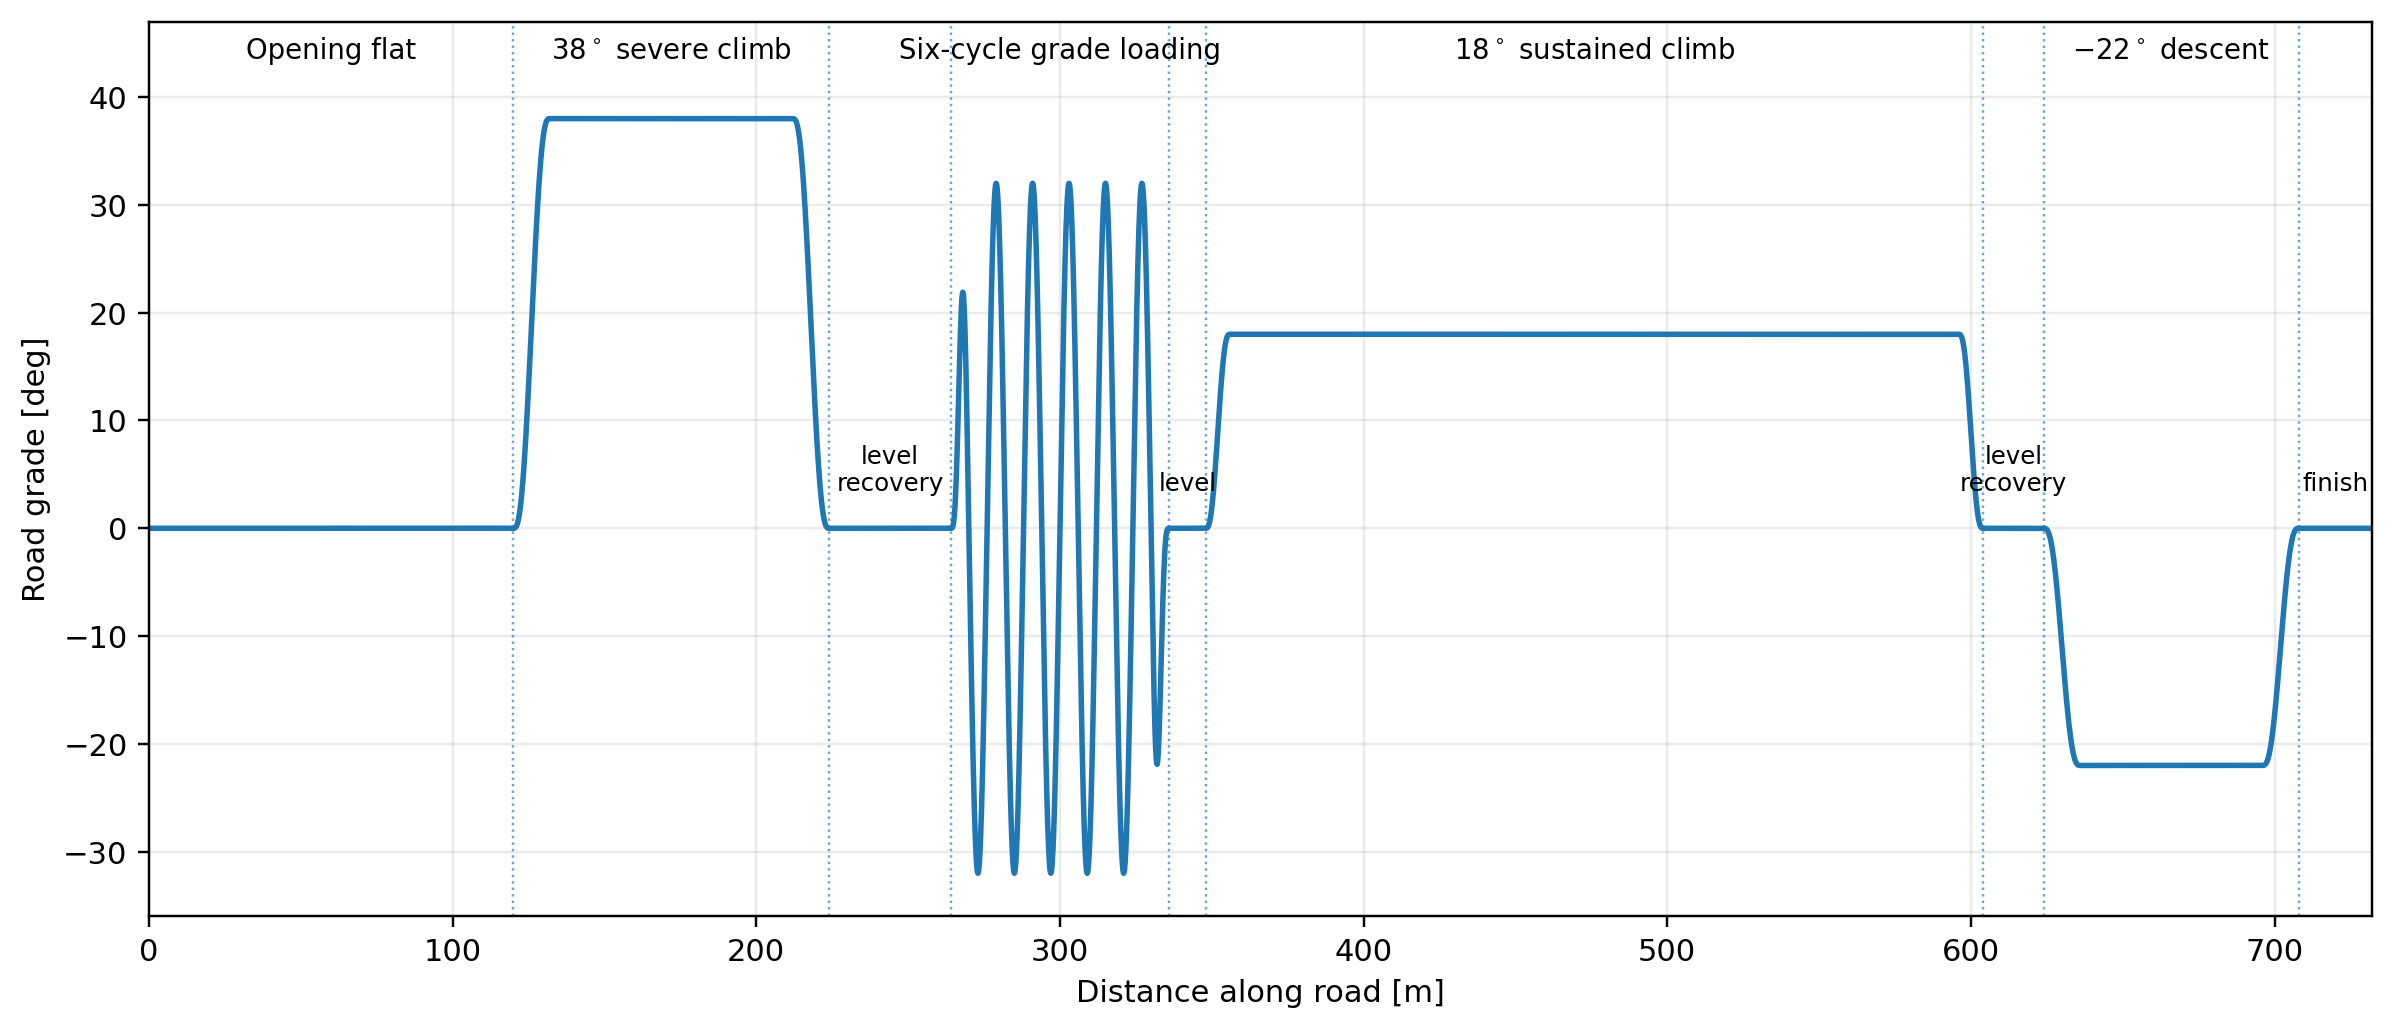
\includegraphics[width=\linewidth]{figures/results/course/common_course_profile.png}
  \caption{Distance-indexed road grade used by every configuration on the
  common \SI{732}{m} course. The first \SI{120}{m} are level. A smooth
  \SI{12}{m} entry leads to an \SI{80}{m} hold at \(38^\circ\), followed by a
  \SI{12}{m} exit and \SI{40}{m} of level recovery. From \SI{264}{m} to
  \SI{336}{m}, the road completes six \SI{12}{m} grade cycles with a peak
  amplitude of \(\pm32^\circ\), followed by \SI{12}{m} of level road. The
  second climb uses an \SI{8}{m} entry, a \SI{240}{m} hold at \(18^\circ\), and
  an \SI{8}{m} exit, followed by \SI{20}{m} of level recovery. The final load
  change is a \(-22^\circ\) descent with \SI{12}{m} entry and exit transitions
  around a \SI{60}{m} constant-grade section, followed by a \SI{24}{m} level
  finish. The cyclic region changes only the longitudinal road grade;
  suspension motion, wheel unloading, tire normal-load variation, and airborne
  vehicle dynamics are not represented.}
  \label{fig:results_course_overview}
\end{figure}

Each part of the road is included to ask a different mechanical question. The
opening flat gives the CVT room to engage and move through its ratio range
before a large road load is introduced. The \(38^\circ\) climb then places a
much larger demand on the drivetrain, allowing limitations in available ratio
or belt traction to appear if the hardware drives the transmission toward
them. After a level recovery, the six-cycle region applies repeated changes in
longitudinal load and tests how much shift motion remains available as those
changes continue. The long \(18^\circ\) climb serves a different purpose: it
holds the load long enough to separate the initial backshift from whatever
interior ratio, engine speed, and climbing speed the coupled system approaches.
The descent reverses the road-grade contribution and allows any corresponding
reverse transfer of power through the drivetrain to emerge from the same
signed mechanics.

Every vehicle has now been given the same engine boundary, vehicle boundary,
starting state, and road. What changes from run to run is selected hardware
inside the CVT. Those configurations are defined in
\Cref{tab:results_course_cases}. The nominal case, R00, is the unmodified Baja
reference CVT of \Cref{app:common_physical_configuration}, using the bilateral
secondary helix topology of \Cref{app:reference_helix_topology}. Every other
row lists only the hardware changed from that baseline; unlisted quantities
retain the reference values. The mass percentages refer to the replaceable
flyweight tip mass rather than the total flyweight mass, and the corresponding
mass moments are changed consistently.

\begin{table}[H]
  \centering\small
  \setlength{\tabcolsep}{4pt}
  \renewcommand{\arraystretch}{1.14}
  \caption{Selected CVT hardware configurations used on the common course.
  Only changes from the nominal R00 reference are listed for the remaining
  cases. Ramp distances are physical coordinates along the ramp, not
  movable-sheave travel.}
  \label{tab:results_course_cases}
  \begin{tabular}{@{}
    >{\raggedright\arraybackslash}p{0.11\linewidth}
    >{\raggedright\arraybackslash}p{\dimexpr0.89\linewidth-2\tabcolsep\relax}@{}}
    \toprule
    Case & Change from R00 \\
    \midrule
    R00 & Unmodified reference configuration; no hardware change. \\
    W85 & Replaceable primary flyweight tip mass reduced to \(85\%\). \\
    P300 & Primary spring stiffness increased to \(3k_p\); installed
      compression reduced so that the spring force matches R00 at the
      low-ratio engagement geometry. \\
    RC10 & Reference ramp retained for the first \SI{10}{mm}, followed by a
      \SI{5}{mm} smooth blend into an arc ending at \(10^\circ\). \\
    R26B7 & Reference ramp retained for the first \SI{10}{mm}, followed by a
      \SI{7}{mm} smooth blend into an arc ending at \(26^\circ\). \\
    RC40L & Reference ramp retained for the first \SI{18}{mm}, followed by a
      \SI{5}{mm} smooth blend into an arc ending at \(40^\circ\). \\
    H28 & Secondary helix angle increased from \(20^\circ\) to \(28^\circ\)
      from the circumferential direction. \\
    U55 & Replaceable primary flyweight tip mass reduced to \(55\%\). \\
    D01 & Tip mass increased to \(130\%\); primary and secondary installed
      spring compressions reduced to \(80\%\); secondary torsional preload
      reduced from \(300^\circ\) to \(240^\circ\); helix angle increased to
      \(28^\circ\). \\
    D02 & Tip mass reduced to \(65\%\) and primary installed spring
      compression increased to \(115\%\). \\
    D02\_M & D02 with the flyweight tip mass restored to the reference value. \\
    D02\_P & D02 with the primary installed spring compression restored to the
      reference value. \\
    D02\_M170 & D02 with the flyweight tip mass increased to \(170\%\) of
      the reference value; elevated primary spring compression retained. \\
    \bottomrule
  \end{tabular}
\end{table}

The cases span several ways of changing the forces and motion inside a
mechanically actuated CVT. W85 changes the flyweight mass properties that
produce the primary centrifugal action. P300 changes the primary spring rate
while matching its force to R00 at the low-ratio engagement geometry, allowing
the spring characteristic to be changed without simply beginning from a
larger or smaller opposing force. RC10, R26B7, and RC40L alter different
portions of the physical ramp followed by the roller, so the effect of changing
that contact geometry can be examined without replacing the flyweight
mechanism itself. H28 makes the corresponding comparison on the secondary by
changing the helix geometry that couples reacted torque to axial motion.

U55, D01, and D02 extend the comparison farther from the nominal hardware. U55
continues the flyweight-mass change to a more severe value, while D01 and D02
combine larger changes in the primary and secondary actuation. They are
included to expose whether the more demanding parts of the road bring out
limitations that are not apparent near the reference configuration. D02\_M and
D02\_P then separate two of the primary-side changes contained in D02 by
restoring, one at a time, the nominal flyweight mass and the nominal primary
spring preload. D02\_M170 extends the mass correction to test how stronger
primary closing affects both clamping and backshift. Together, the set
provides several distinct mechanical routes
away from the reference before any of their course responses are interpreted.


\subsection{Launch and the Shape of the Shift Curve}
\label{sec:results_launch_upshift}

The road begins with \SI{120}{m} of level ground. Before the later changes in
grade disturb the drivetrain, this opening lets each CVT engage and begin its
upshift from the common initial state. Plotting primary speed against secondary
speed gives the familiar shift-curve view used in practical CVT tuning
\citep{Aaen2007,Skinner2020}, but here no speed curve is prescribed. Each
trajectory follows from the actuator geometry and spring loading acting
through the belt, secondary, and accelerating vehicle.
\Cref{fig:results_shift_curve_shape} shows this response for six primary-side
configurations, from launch at zero secondary speed to just before the first hill, including
their low-ratio motion, free shift, and any high-ratio motion reached along
the way.

The low-ratio limit is the lower end of engaged shift travel, where the
secondary is fully closed against its stop. The high-ratio limit is reached
when the primary closes against its upper stop
(\Cref{sec:low_ratio_supported_regime,sec:upper_primary_stop_regime}). The
dashed lines show the no-slip shaft-speed relations at those two fixed
geometries. While a stop holds the geometry and both contacts stick, the
shafts accelerate along its line; the disengaged and slipping parts of launch
need not follow either relation.

\begin{figure}[H]
  \centering
  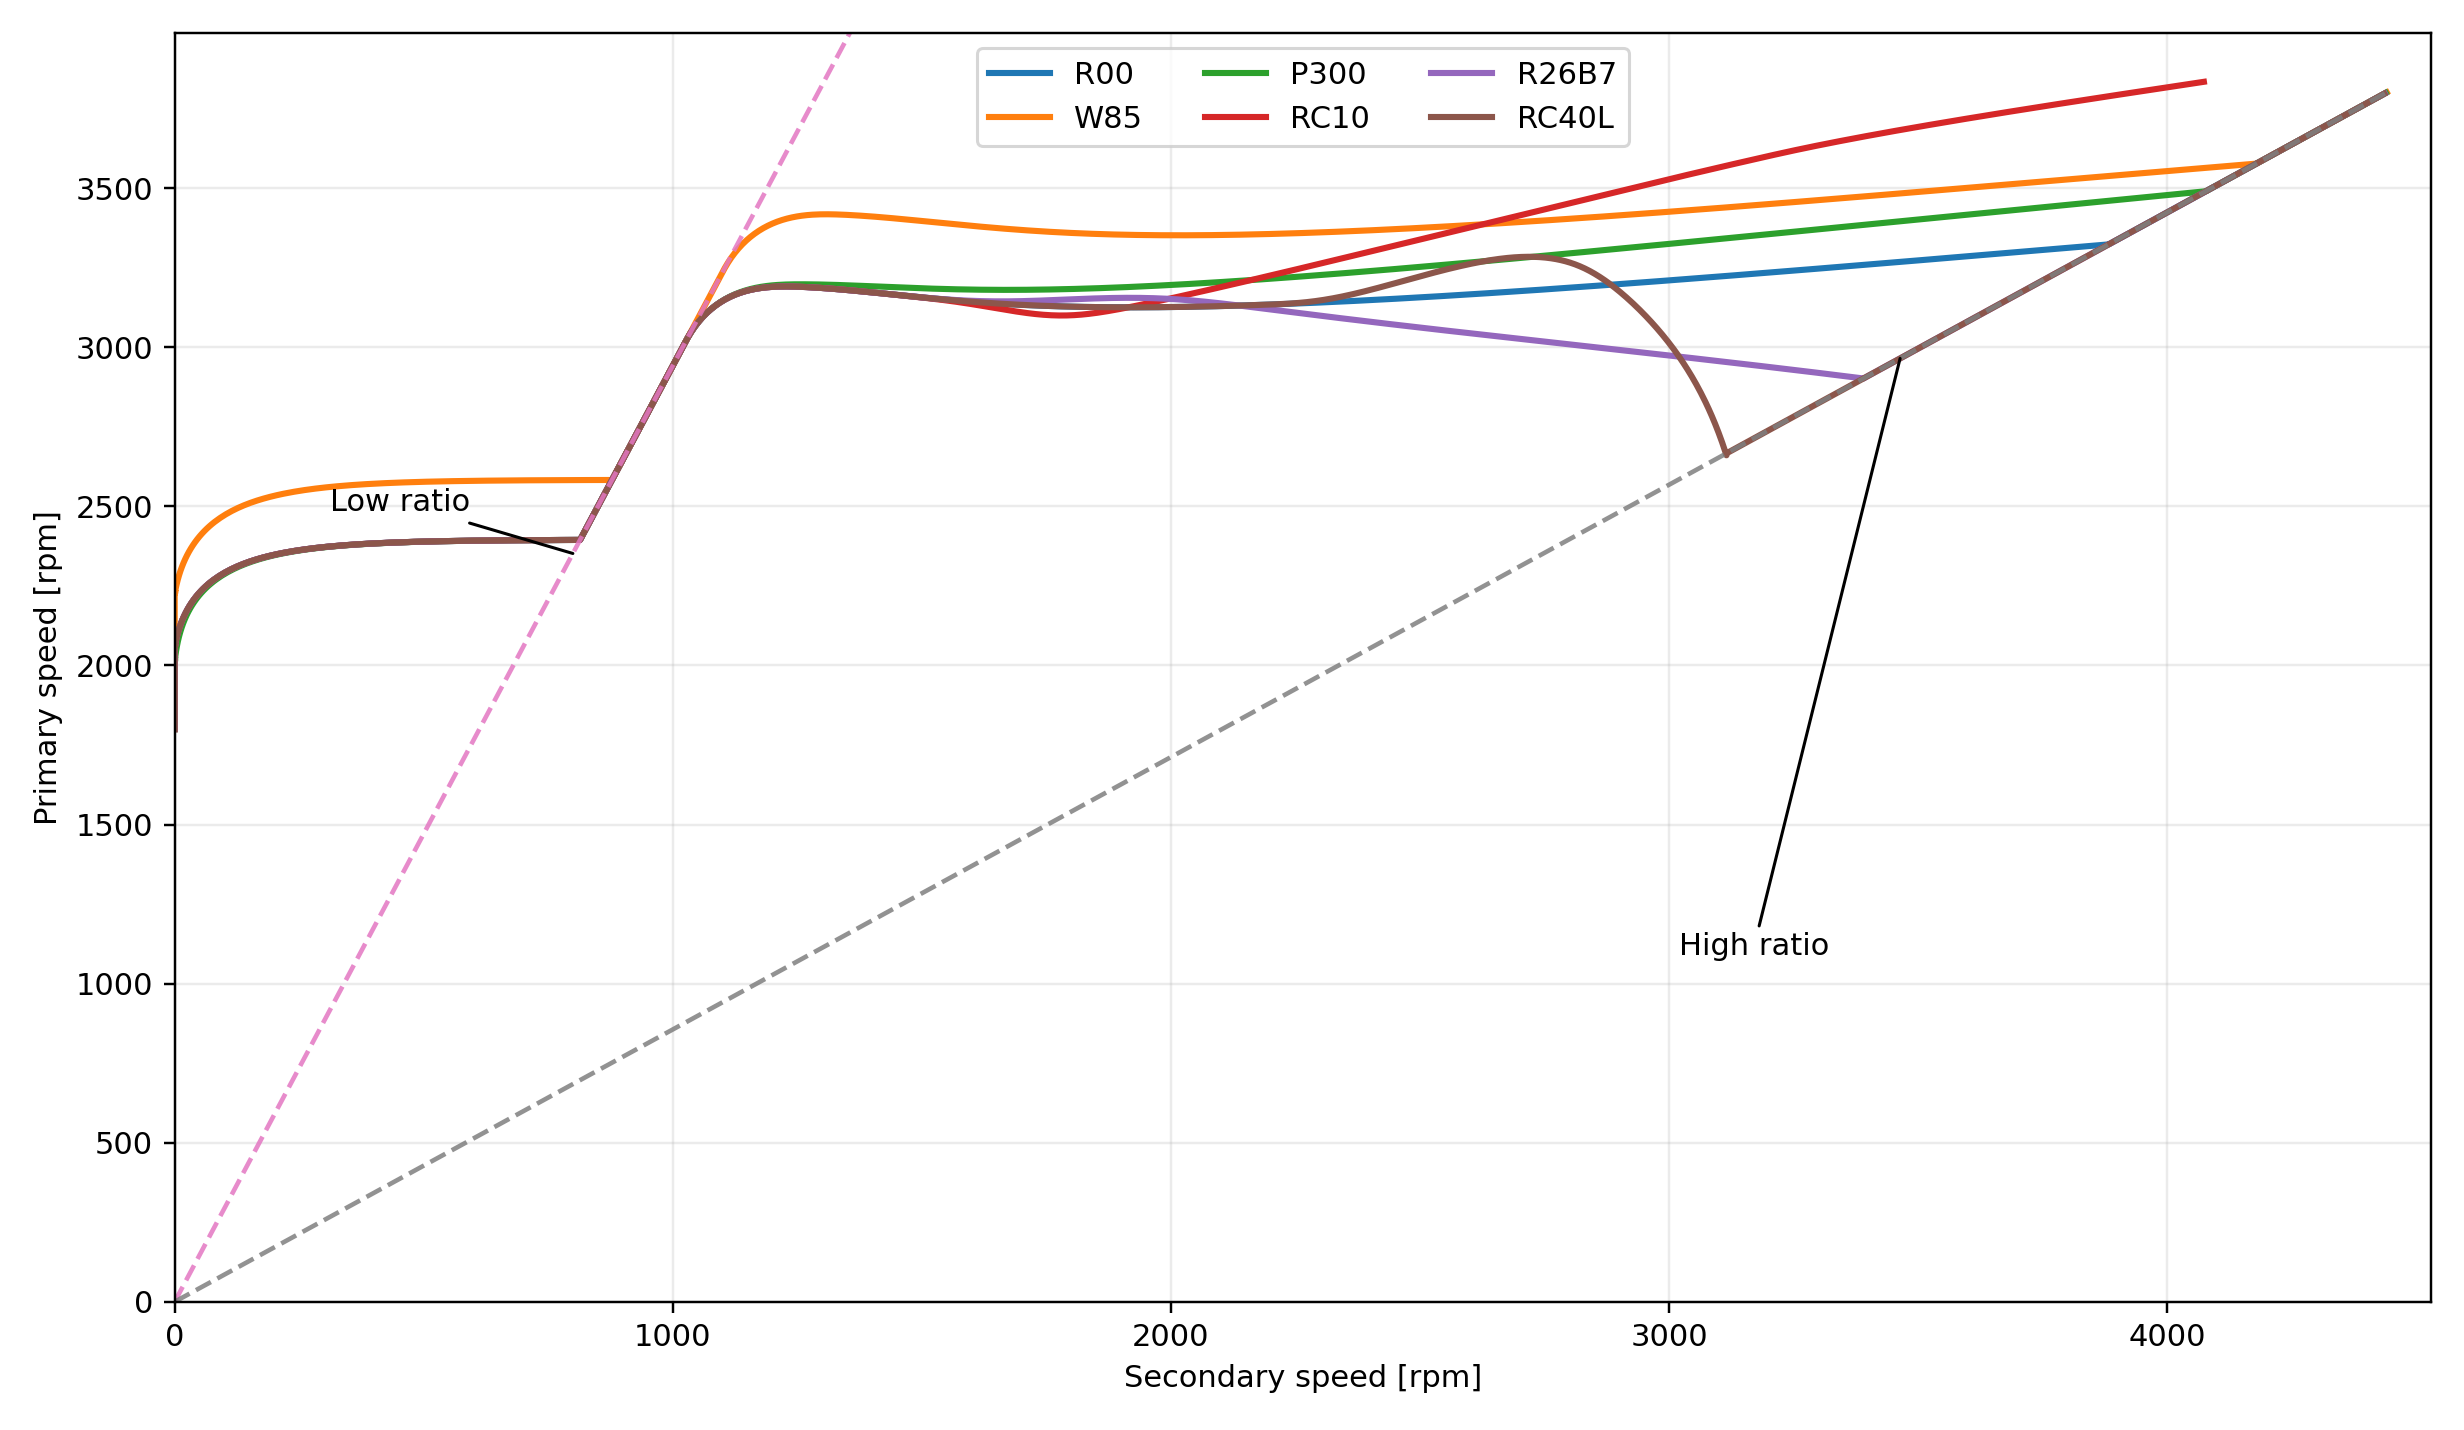
\includegraphics[width=\linewidth]{figures/results/course/opening_free_shift_characteristics.png}
  \caption{Complete opening-flat shift curves for the six selected primary
  hardware configurations, from the initial state through the last recorded
  point before \SI{120}{m}. The solid curves retain the initial disengaged
  motion, launch slip, supported motion, and free shift. The dashed lines are the no-slip speed
  relations at the geometric low- and high-ratio limits.}
  \label{fig:results_shift_curve_shape}
\end{figure}

W85 gives the most familiar change. Reducing the replaceable flyweight tip
mass weakens the speed-dependent centrifugal closing action at a given primary
speed. The transmission therefore has to reach a higher primary speed before a
similar sequence of axial balances can be recovered. The result is not an
exact vertical translation, because every force and inertia term continues to
evolve with the trajectory, but much of the R00 progression is reproduced at
a higher working speed. Between \(20\%\) and \(80\%\) of the available engaged
shift travel, W85 changes from approximately \(3393\) to
\(3447~\mathrm{rpm}\), compared with approximately \(3169\) to
\(3205~\mathrm{rpm}\) for R00. This is the classical lighter-flyweight effect.
The leading speed-dependent contribution appears explicitly
in \Cref{eq:primary_flyweight_axial_force} through
\(\tfrac{1}{2}\omega_p^2\,dJ_{f,p}/dx_p\).

P300 begins much closer to the reference but separates for a different reason.
Its installed compression is reduced so that
\Cref{eq:primary_spring_force} gives the same primary spring opening force as
R00 at the low-ratio engagement geometry, as shown in
\Cref{fig:results_shift_curve_mechanics}(a). Early in the shift, the two cases
therefore begin from nearly the same competition between flyweight closing
action and spring opposition. As the primary continues to close, however, the
three-times-greater spring rate makes that opposition grow more rapidly. The
later sheave motion consequently slows relative to R00. Secondary speed can
continue to rise while less ratio change is produced, giving the primary and
its attached engine more opportunity to accelerate relative to the secondary.
The curve therefore peels upward as the shift proceeds, reaching approximately
\(3336~\mathrm{rpm}\) by \(80\%\) travel even though it began near the R00
operating point. Matching the spring force at one position has not matched the
spring characteristic through the rest of the shift.

\begin{figure}[H]
  \centering
  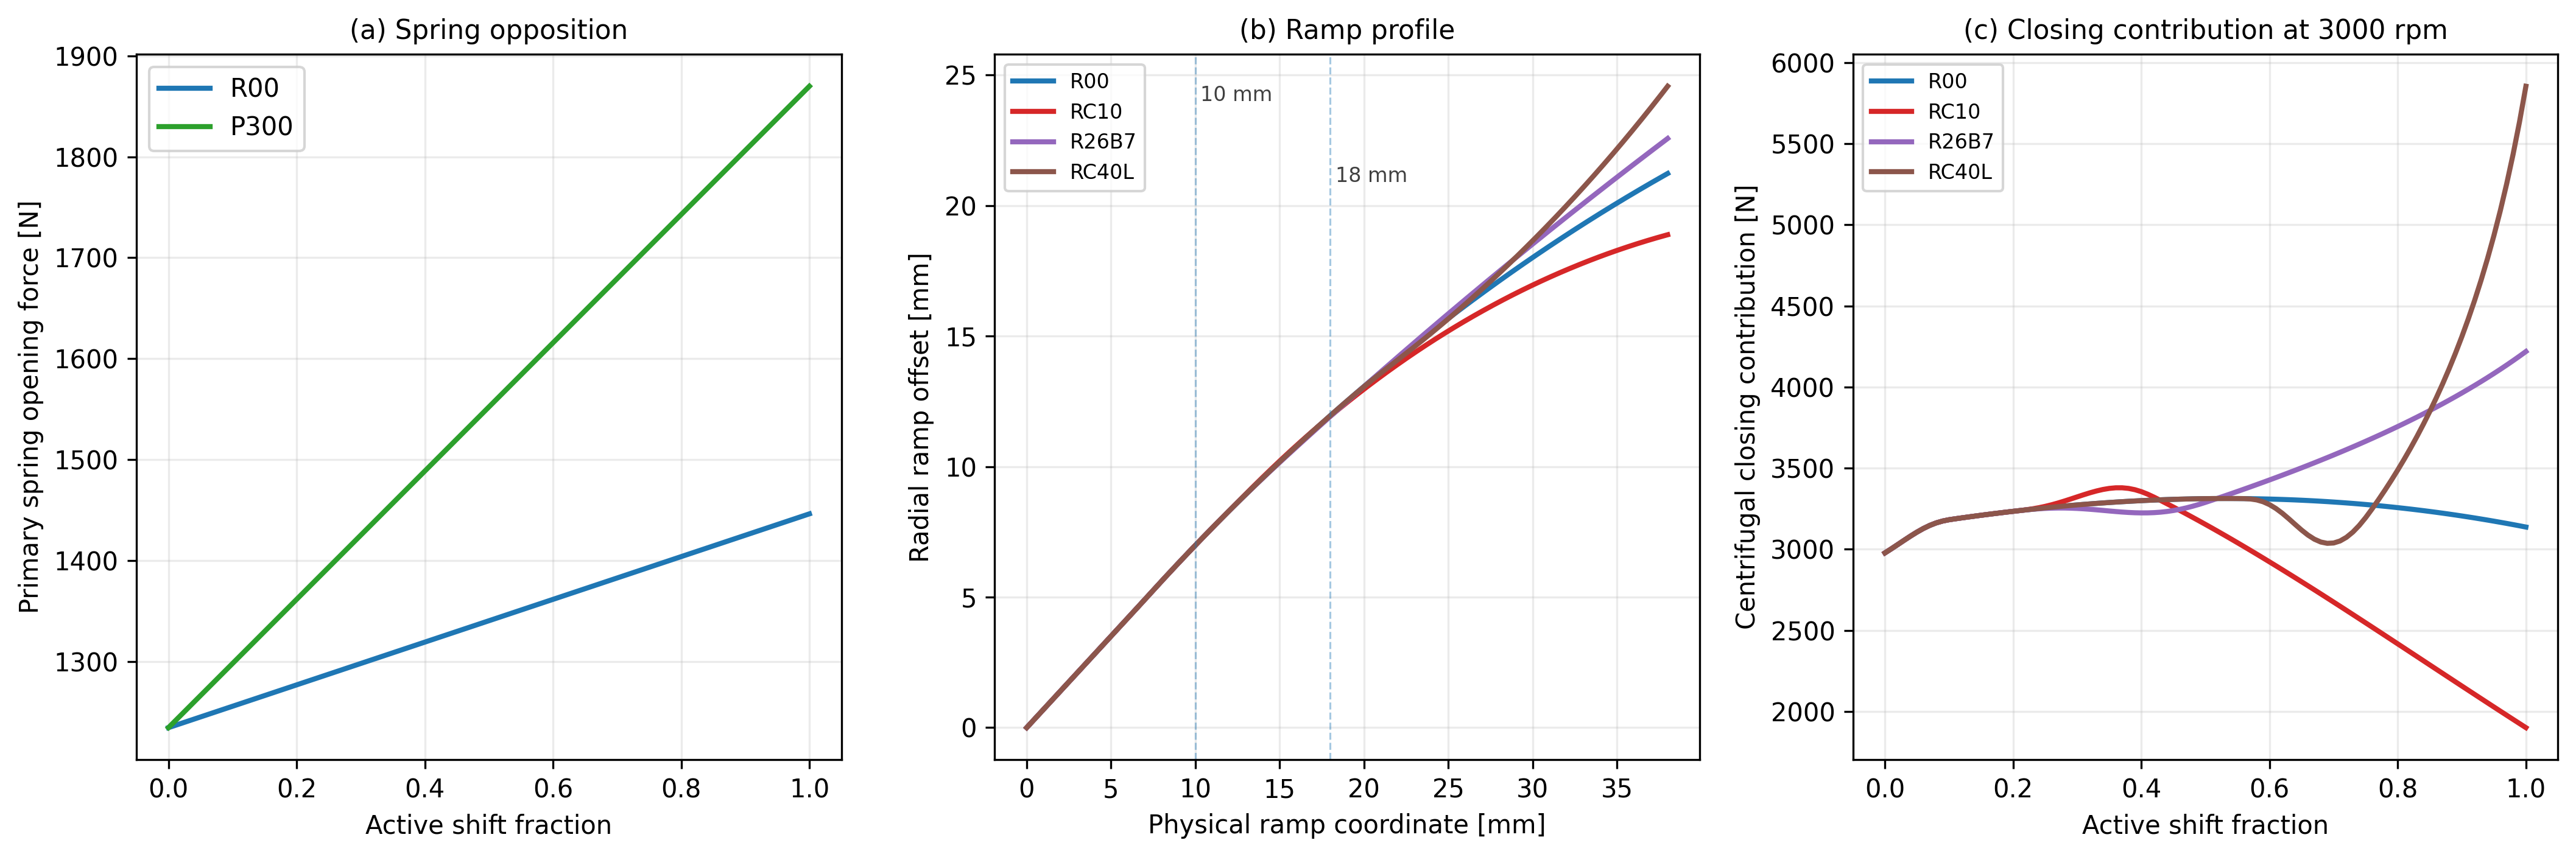
\includegraphics[width=\linewidth]{figures/results/course/shift_curve_mechanical_causes.png}
  \caption{Mechanical origin of the selected shift-curve changes. (a) Primary
  spring opening force for R00 and P300, matched at the low-ratio engagement
  geometry. (b) Physical ramp profiles: RC10 and R26B7 preserve the first
  \SI{10}{mm} of the reference ramp, while RC40L preserves the first
  \SI{18}{mm}; these distances are ramp coordinates rather than
  movable-sheave travel. (c) Leading centrifugal closing contribution at the
  same \(3000~\mathrm{rpm}\) primary speed. The complete actuator also retains
  the corresponding motion-ratio and flyweight-inertia terms, so panel (c)
  isolates one contribution rather than replacing the full dynamic force law.
  In (a) and (c), active shift fraction runs from zero at the low-ratio seat to
  one at the upper primary stop.}
  \label{fig:results_shift_curve_mechanics}
\end{figure}

The spring case changes a force that varies linearly with displacement. The
ramp cases instead change the geometry through which the roller moves, so the
relationship between flyweight motion and axial closing force can vary
nonlinearly as different parts of the profile are reached. The changed
profiles in \Cref{fig:results_shift_curve_mechanics}(b) therefore produce
different closing-force variations even at the same primary speed, as
panel~(c) illustrates at \(3000~\mathrm{rpm}\).

That difference in how the hardware varies through travel is visible in the
three ramp trajectories. RC10 and R26B7 preserve the same early ramp as R00,
so their initial free-shift response remains close to the reference. Once the
roller reaches the modified region, the closing contribution no longer has to
change monotonically or even in the same direction as the reference. RC10 first
drops slightly and then turns sharply upward, reaching approximately
\(3655~\mathrm{rpm}\) at \(80\%\) travel. R26B7 develops the opposite tendency
and falls to approximately \(3013~\mathrm{rpm}\). RC40L leaves a longer portion
of the reference profile untouched; its trajectory remains essentially
coincident with R00 through the earlier shift before developing a distinct
late shoulder and downturn. Unlike the linear spring-rate change, a ramp
change can therefore reshape the working-speed characteristic differently in
different parts of the same shift.

The shift curves also show that the upper primary stop is reached at different
points in the opening acceleration. RC10 is still freely shifting when the
first hill arrives, whereas the other five curves have already joined the
high-ratio line. With the stop geometry unchanged, these different arrivals
follow from the actuator characteristics acting through the same belt,
secondary, engine boundary, and vehicle.

One ambiguity remains when a case has not reached the upper stop before the
first hill arrives. The common course deliberately changes grade after
\SI{120}{m}, so an incomplete opening shift by itself cannot distinguish a
slow approach to high ratio from an interior balance that would persist on
level ground. The more extreme flyweight-mass reduction in U55 also leaves its
opening shift incomplete. To see whether it simply needs a longer level road,
R00 and U55 were also run over a separate \SI{800}{m} flat.

R00 again reaches the \SI{19.05}{mm} upper stop near \SI{64.9}{m}. U55 instead
approaches an interior shift position near \SI{14.90}{mm}, changing by less
than \SI{0.001}{mm} over the final \SI{10}{s}. Under the observed flat-road
load, the reduced primary closing action therefore approaches a balance with
the opposing spring, belt, and secondary reactions before the high-ratio stop
is reached. The finite run does not prove that U55 could never move farther,
but it shows that its incomplete shift on the common course is not simply
caused by the \(38^\circ\) hill arriving a few metres too soon.

The opening-flat cases therefore make several familiar tuning ideas more
precise. A lighter flyweight can make much of the same shift progression occur
at a higher primary speed. A stiffer primary spring can leave the beginning of
that progression nearly unchanged while increasingly slowing the later ratio
motion, allowing engine speed to rise relative to the secondary. Changing the
ramp can alter the same balance nonlinearly and only over the portions of
travel where the new geometry is encountered. Those different states are then
carried directly into the first severe climb, where the question changes from
how the hardware shapes the upshift to what limits the transmission when the
road demands a large backshift.

\subsection{A Severe Climb Separates Poor Shifting from Loss of Traction}
\label{sec:results_backshift}

The first climb increases the gravitational resistance to forward motion,
so the wheels need more torque to sustain the vehicle's speed. If the ratio
stays fixed while the belt sticks, slowing the vehicle also slows the engine,
potentially taking it away from the speeds at which it supplies useful power.
Gearing down allows the same transmitted power to provide more wheel torque
at a lower wheel speed, while keeping the engine turning faster relative to
the vehicle. Backshifting serves that purpose by moving the belt inward on
the primary and outward on the secondary. The secondary helix provides a
physical connection between torque loading and this motion: the torque it
reacts produces axial closing thrust alongside the spring force
(\Cref{eq:secondary_helix_force_conversion}). At the same time, falling
primary speed weakens the centrifugal action holding the primary closed.
Through the belt, these changes can open the primary and close the secondary,
producing the required backshift.

How much this helps the vehicle depends on both the ratio reached and the
traction available to transmit torque through the belt.
\Cref{fig:results_severe_hill_response} therefore brings together shift
position, primary speed, and vehicle speed for R00 and the two adverse cases,
D01 and D02. The road-position axis places them under the same local grade,
while retaining the different states inherited from the opening flat. R00
provides the reference response: it leaves the high-ratio stop, backshifts to
the low-ratio seat, and continues climbing. After the brief seating
transition, both contacts stick and the vehicle approaches approximately
\SI{3.77}{m/s}. Reaching the end of backshift travel has limited the ratio,
but has not prevented torque transmission.

\begin{figure}[H]
  \centering
  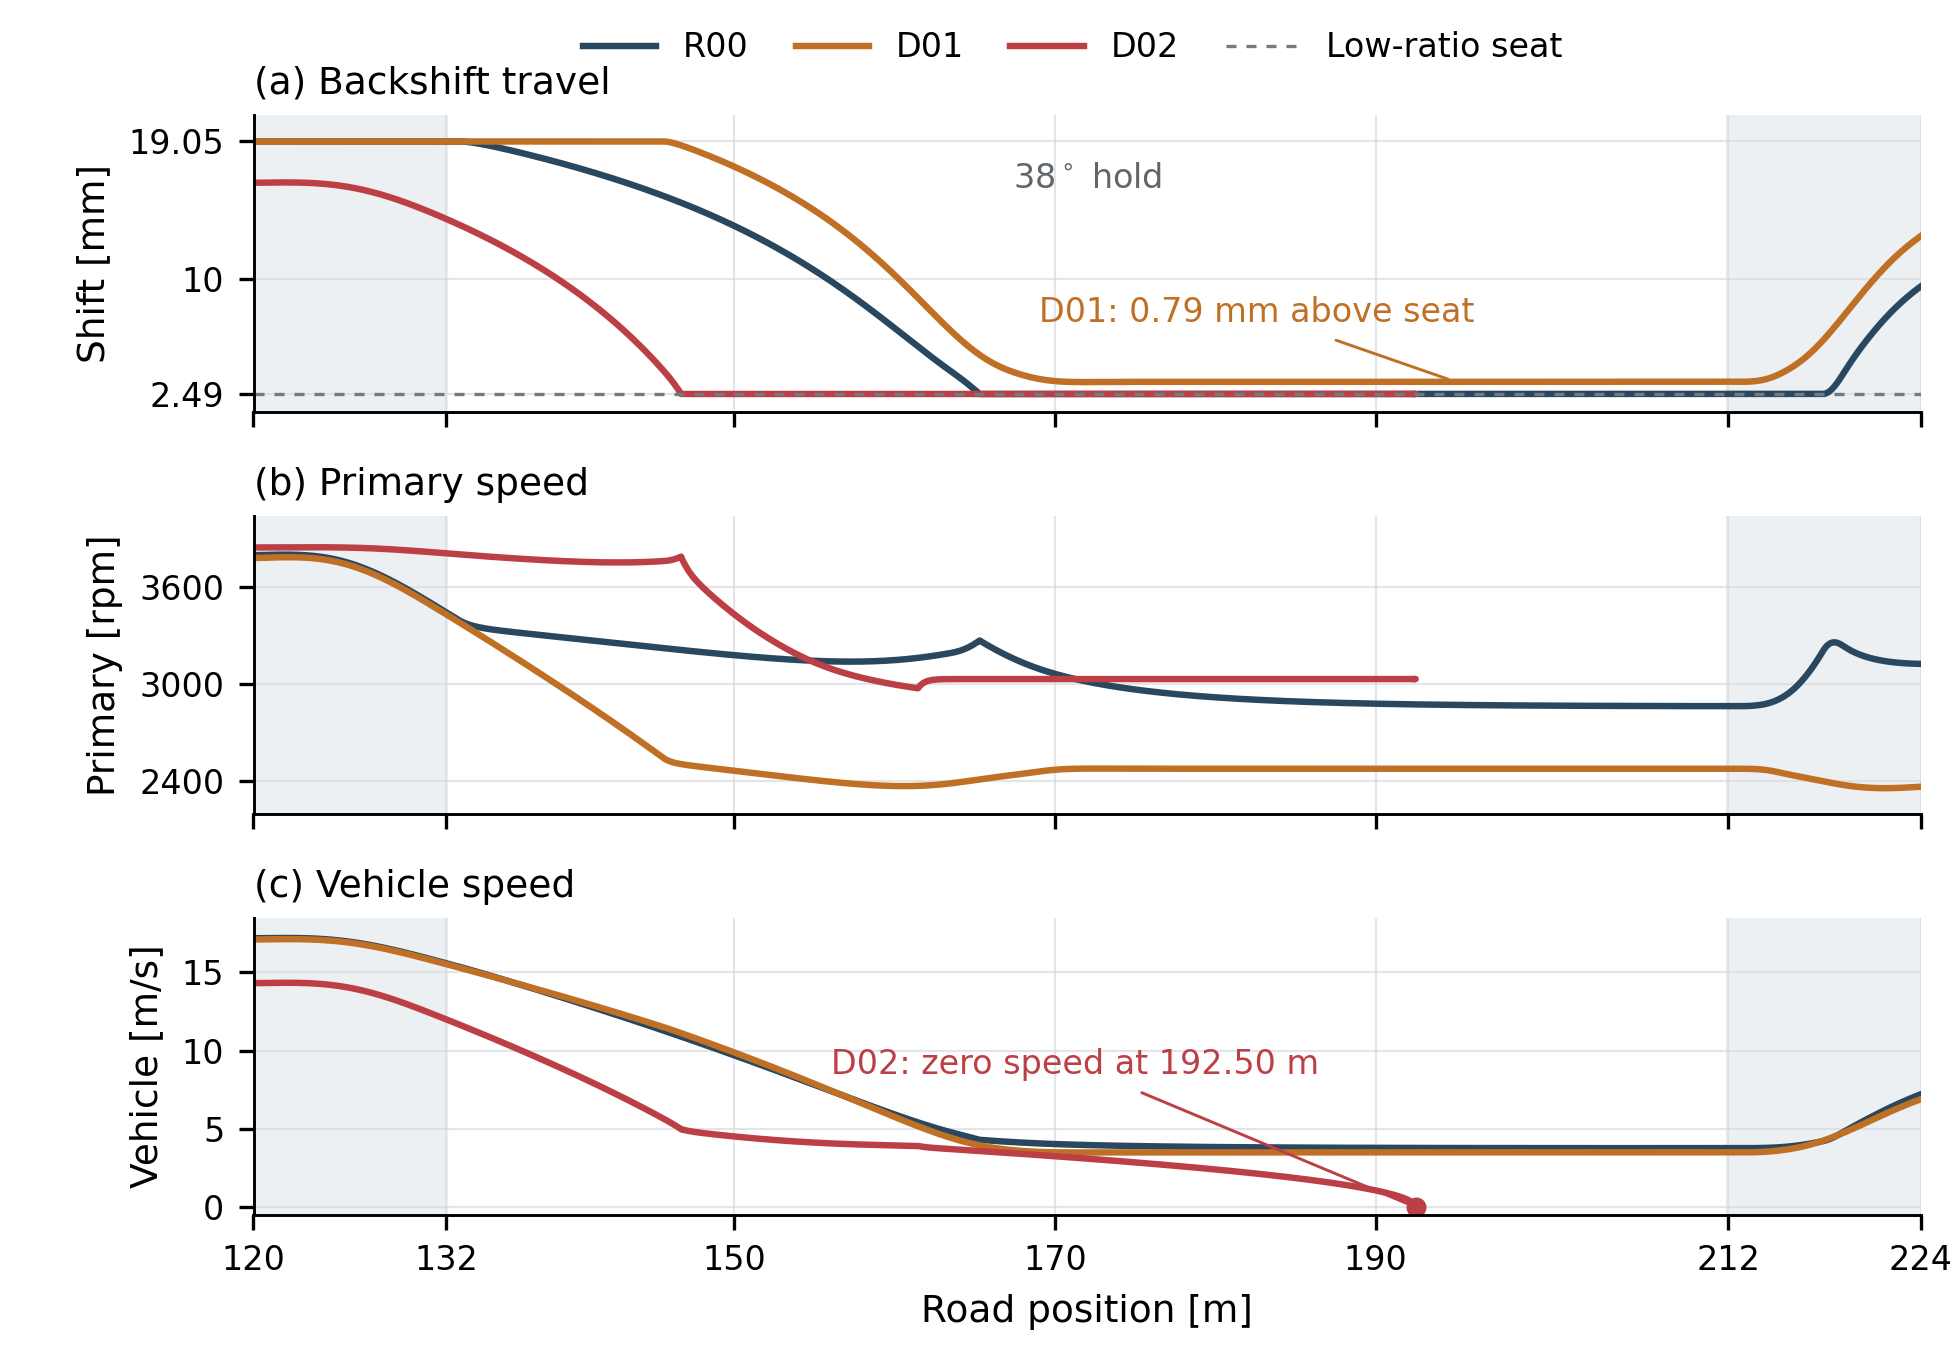
\includegraphics[width=\linewidth]{figures/results/course/severe_hill_response.png}
  \caption{Response to the first severe climb. The shaded bands mark the
  entry and exit tapers; the intervening road holds \(38^\circ\). The dashed
  line in (a) marks the low-ratio seat. All three D02 traces end at its first
  zero vehicle speed, near \SI{192.50}{m}. Equal road
  position means equal imposed grade, not equal elapsed time or inherited
  state.}
  \label{fig:results_severe_hill_response}
\end{figure}

D01 remains at the high-ratio stop farther into the climb. While the geometry
is held and the belt sticks, engine speed must fall with vehicle speed. Its
heavier primary tips and reduced primary spring opposition favour primary
closure, while the reduced secondary spring loading and changed helix weaken
the secondary closing action that favours backshift. Near \SI{200}{m}, D01
still has approximately \SI{0.79}{mm} of backshift travel available and runs
near \(2477~\mathrm{rpm}\), where the supplied engine boundary delivers less
power than in R00. Both belt contacts continue sticking throughout the hill,
and the vehicle still climbs, but at a lower speed. Its difficulty is the
ratio and engine operating condition reached under load; primary traction has
not been exhausted.

D02 reaches the low-ratio seat near \SI{146.68}{m}, so its later loss of
progress begins after the available backshift has already been used. The
secondary has completed its closing travel, but the primary must still squeeze
the belt strongly enough to transmit torque. D02's light tips provide less
centrifugal closing action, while its elevated primary spring compression
increases the opposing opening force. As established in
\Cref{sec:low_ratio_supported_regime}, the secondary is held against its
closing stop while the primary axial balance still determines clamping. At this fixed
geometry, primary spring opposition stays constant, but the centrifugal
closing contribution decreases as primary speed falls. The remaining closing
force must balance the belt's opening reaction, so the primary normal load
falls with it
(\Cref{eq:primary_flyweight_axial_force,eq:primary_belt_axial_reaction}).
For D02, the normal load decreases from about \SI{3.49}{kN} just after seating
to \SI{1.05}{kN} before sustained slip begins. Loading carried by the
secondary stop does not add to the belt normal force or supply extra traction.

Sticking can continue only while the required tangential force remains
within the static capacity supported by that normal load. While a contact
sticks, \(\lvert\lambda_j\rvert/\mu_s\)
measures the fraction of its available static traction required by the
coupled motion; unity is the sticking limit. In
\Cref{fig:results_d02_traction_power}(a), the primary reaches this limit near
\SI{17.83}{s} after launch, while the secondary remains below its own limit
and continues sticking. The primary then slides relative to the belt. Its
speed recovers slightly toward \(3032~\mathrm{rpm}\), but the vehicle keeps
slowing, as already seen in \Cref{fig:results_severe_hill_response}. Following
the power in panel~(b) explains how engine rotation can continue while forward
progress is lost.

\begin{figure}[H]
  \centering
  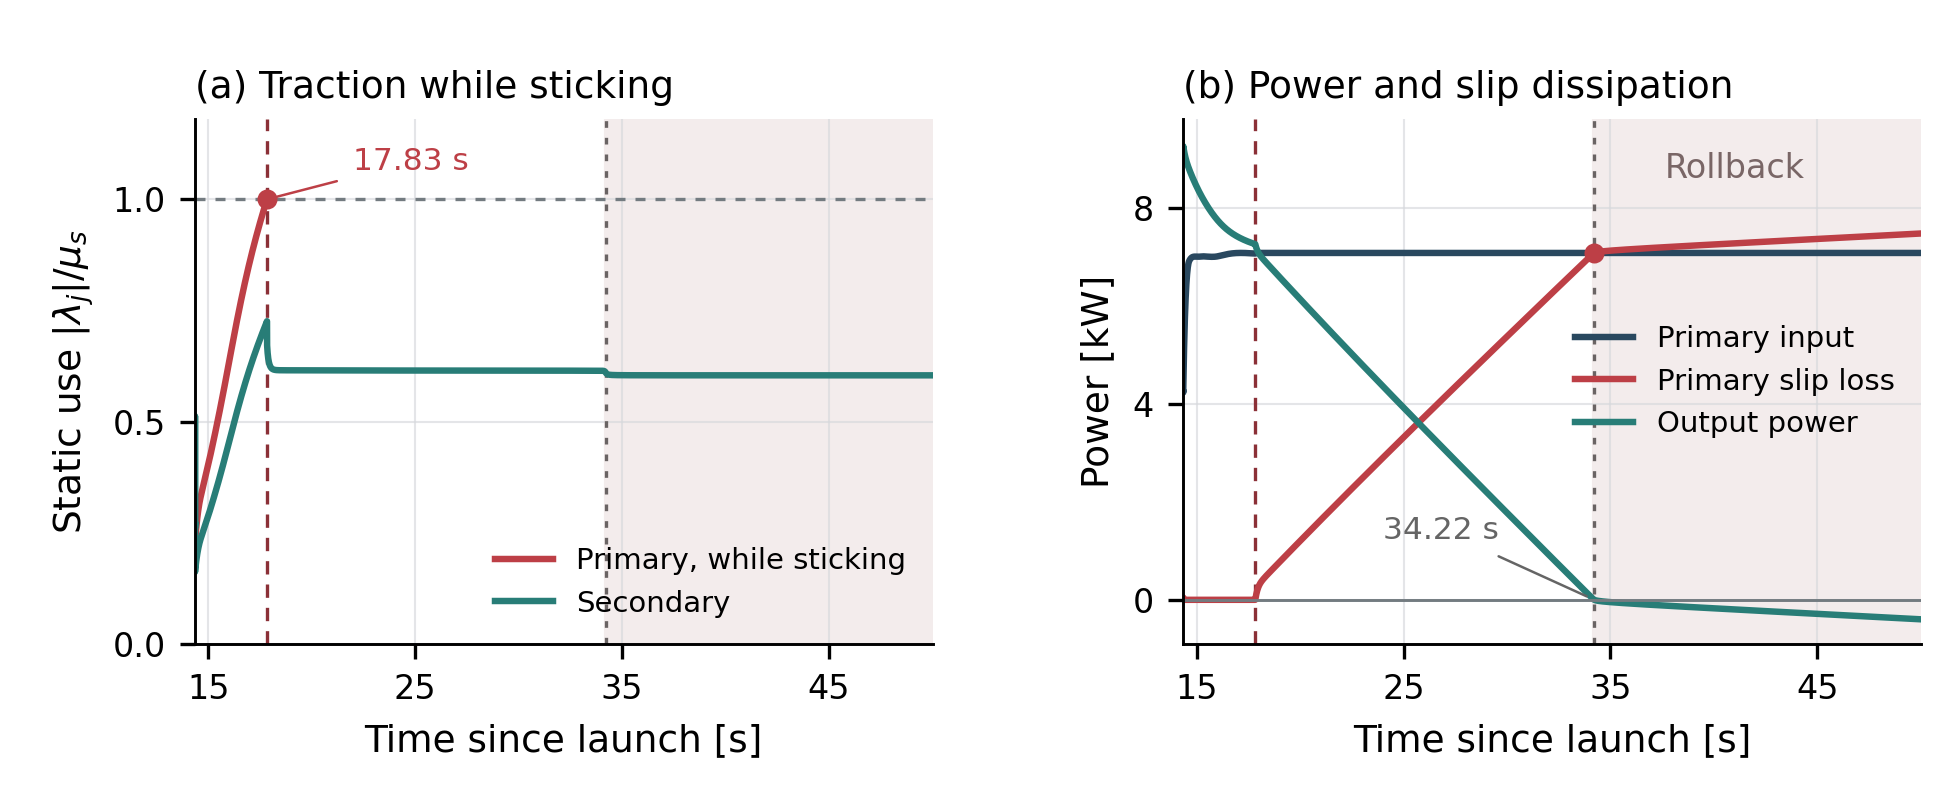
\includegraphics[width=\linewidth]{figures/results/course/d02_traction_power.png}
  \caption{D02 from arrival at the low-ratio seat through the retained
  rollback. (a) Fraction of static traction used while each contact sticks;
  the primary trace ends when sustained sliding begins. (b) Primary boundary
  input, primary slip dissipation, and signed output power. Positive output
  power leaves the CVT; negative output power enters from the vehicle side.
  Vertical markers identify primary traction loss and the first zero vehicle
  speed, with rollback shaded. During transients, differences between input,
  output, and dissipation also include changes in stored mechanical energy.}
  \label{fig:results_d02_traction_power}
\end{figure}

Near \SI{34.22}{s}, the vehicle reaches zero speed while the primary still
turns near \(3032~\mathrm{rpm}\). Approximately \SI{7.07}{kW} enters through
the primary boundary, and essentially the same power is dissipated in primary
slip; useful output power has fallen to zero. The vehicle subsequently rolls
back. Output power then becomes negative, because the descending vehicle
supplies power into the CVT, and primary slip dissipation can exceed the
engine input. For the remainder of the simulated interval, the vehicle
continues rolling backward while the primary rotates forward and slides
against the belt.

Preventing this loss of grip requires sufficient primary normal load at the
low ratio D02 has already reached. At the seated geometry, the primary force
balance relates that load to the difference between centrifugal closing and
spring opposition. D02\_M restores the reference tip mass and its
associated mass moments, strengthening centrifugal closing while retaining
D02's elevated primary spring compression. The same mass correction is also
extended to \(170\%\) of the reference tip mass in D02\_M170, with
corresponding mass moments and the same spring compression. D02\_P retains the light tips but
restores the reference spring compression, reducing the opening force opposing
the flyweights without changing the spring rate. A larger
remaining closing force supports a larger primary belt normal load, and the
unchanged friction coefficient then permits a larger tangential force before
sticking is lost. These are two physical ways to correct the same clamping
weakness.

The changed primary forces also alter the backshift shown in
\Cref{fig:results_d02_hill_repairs}(a). Both D02\_M and D02\_P reach the
same low-ratio seat as D02 and remain there through the rest of the constant
\(38^\circ\) climb, whereas D02\_M170 retains unused backshift travel.

\begin{figure}[H]
  \centering
  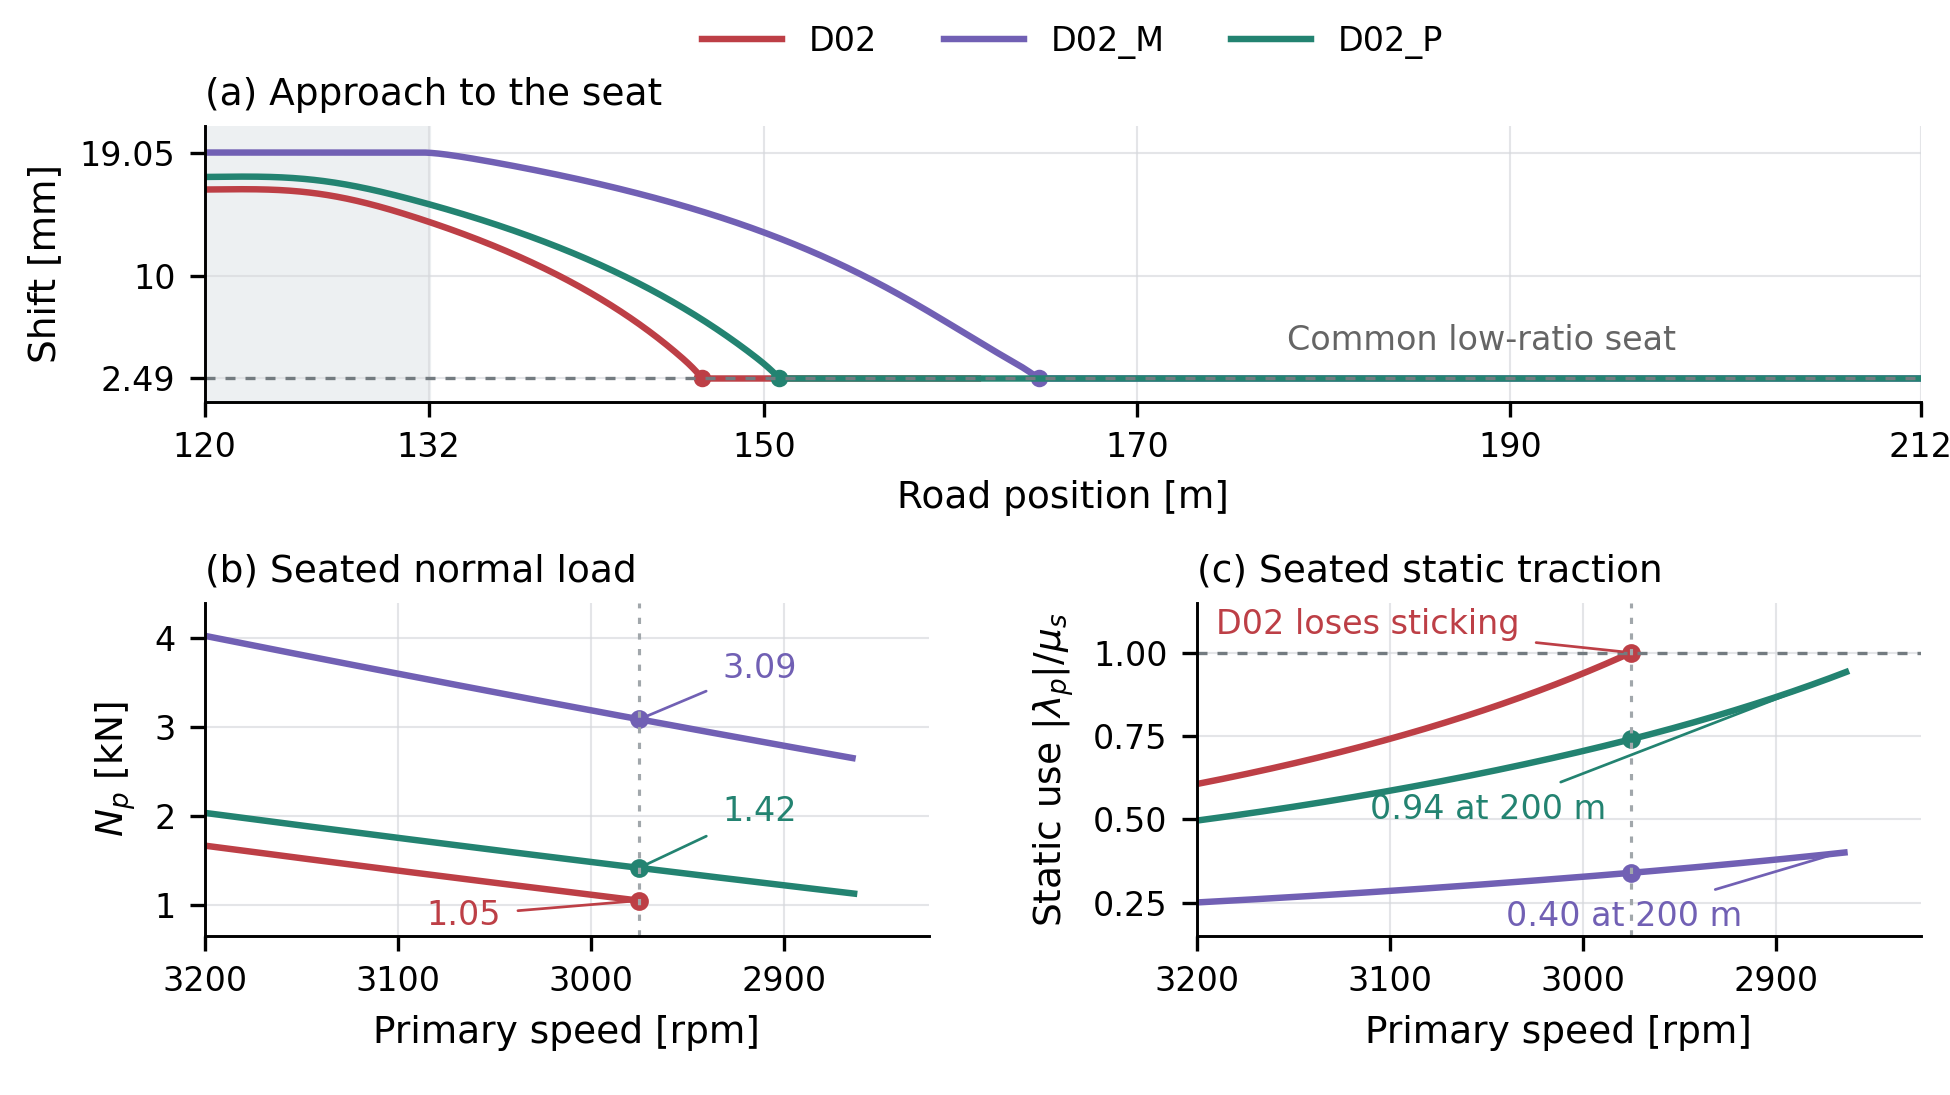
\includegraphics[width=\linewidth]{figures/results/course/d02_hill_repairs.png}
  \caption{Clamping and backshift under the three primary-side corrections.
  (a) Approach to the common low-ratio seat, with the hill-entry taper shaded.
  Equal road position retains the different states inherited from the opening
  flat. (b) Total primary normal load and (c) static utilization during seated
  sticking on the \(38^\circ\) hold, after the seating transitions. Markers
  in (b,c) identify the comparison near \(2975~\mathrm{rpm}\); the repair
  utilization annotations refer to states near \SI{200}{m}. D02 traces end
  at sustained primary slip onset. D02\_M170 is absent from (b,c) because
  it does not reach the seat on the constant \(38^\circ\) climb.}
  \label{fig:results_d02_hill_repairs}
\end{figure}

The stronger mass correction in D02\_M170 maintains ample clamping, but its
centrifugal closing also opposes the primary opening needed for backshift.
Both contacts stick throughout the constant \(38^\circ\) climb, yet the
transmission remains above the seat in panel~(a). Near \SI{200}{m}, the
primary uses only about \(0.20\) of its static capacity, while the engine
turns near \(2660~\mathrm{rpm}\), compared with \(2870~\mathrm{rpm}\) in
D02\_M. At this lower speed the supplied engine boundary delivers less power,
and the vehicle climbs at approximately \SI{3.66}{m/s} instead of
\SI{3.77}{m/s}. D02\_M170 still completes the course, but the stronger correction
introduces the same kind of unfavourable ratio and engine operating condition
seen in D01.

D02\_M and D02\_P restore grip while still allowing full backshift.
Because they reach the same low-ratio seat as D02, their clamping can be
compared at a common pulley geometry. Panels~(b) and (c) make this comparison
at matching primary speeds, showing normal load and the fraction of static
capacity used as each case slows on the constant \(38^\circ\) slope.
Matching states occur at different times and road positions in each run.

At the marked speed, the primary must transmit approximately \SI{683}{N}
of tangential force in each case. For D02, this demand has reached the
static limit \(\mu_sN_p\). Restoring the tip mass in D02\_M strengthens
centrifugal closing, while reducing the spring compression in D02\_P leaves
less opening force to oppose it. Both corrections therefore produce greater
normal loads in panel~(b), with the larger increase in D02\_M. This additional
normal load raises the available static force, so the same tangential demand
uses a smaller fraction of that capacity in panel~(c). Both repairs retain
grip below D02's slip-onset speed, even as their own normal loads fall and
the fractions of capacity used rise.

The two repairs nevertheless leave different margins against slip. Near
\SI{200}{m}, D02\_M uses about \(0.40\) of its primary static capacity,
leaving a substantial reserve, whereas D02\_P uses about \(0.94\) and is
close to its traction limit. Yet both climb near \SI{3.77}{m/s} at the same
low-ratio seat. Both already transmit the required force without sliding.
The larger normal load in D02\_M increases the force the primary could
support at that state, but does not itself supply more power to the wheels.

The hill has separated an unfavourable ratio and engine speed with unused
backshift travel from a loss of belt traction after full backshift. Following
the latter failure through the primary force balance identifies two ways to
restore enough clamping, with different remaining traction reserves. The
stronger mass correction shows why that improvement cannot be judged from
clamping alone: the same closing action also changes backshift, engine speed,
and climbing speed.

\FloatBarrier

\subsection{Repeated Loading and Upper-Stop Support}
\label{sec:results_cyclic_loading}

After the first hill, the level recovery allows the vehicle to regain speed
and the CVT to upshift. The next road feature repeatedly reverses the
gravitational contribution to the load: six \SI{12}{m} grade cycles alternate
between climbing and descending. Increased resistance can again promote
backshift through the torque-sensitive secondary, while the reduction in
load gives primary closing action more opportunity to upshift. Repeating
these changes tests whether the sheaves continue moving or become held at a
travel limit as the vehicle accelerates. This remains a longitudinal-load
test; suspension motion, wheel unloading and airborne dynamics are not
represented.

The primary spring and ramp changes examined in
\Cref{sec:results_launch_upshift} also change the recovery from the hill and
the state carried into these cycles. \Cref{fig:results_cyclic_support}
compares R00 with P300 and the two ramp cases, R26B7 and RC10. R26B7 has
already returned to the common \SI{19.05}{mm} upper primary stop before
the first cycle begins. The other three enter below it, with room for
further closure. Shift position shows whether that room is used; the stop
reaction shows when the hardware carries closing load instead of allowing
further motion.

\begin{figure}[H]
  \centering
  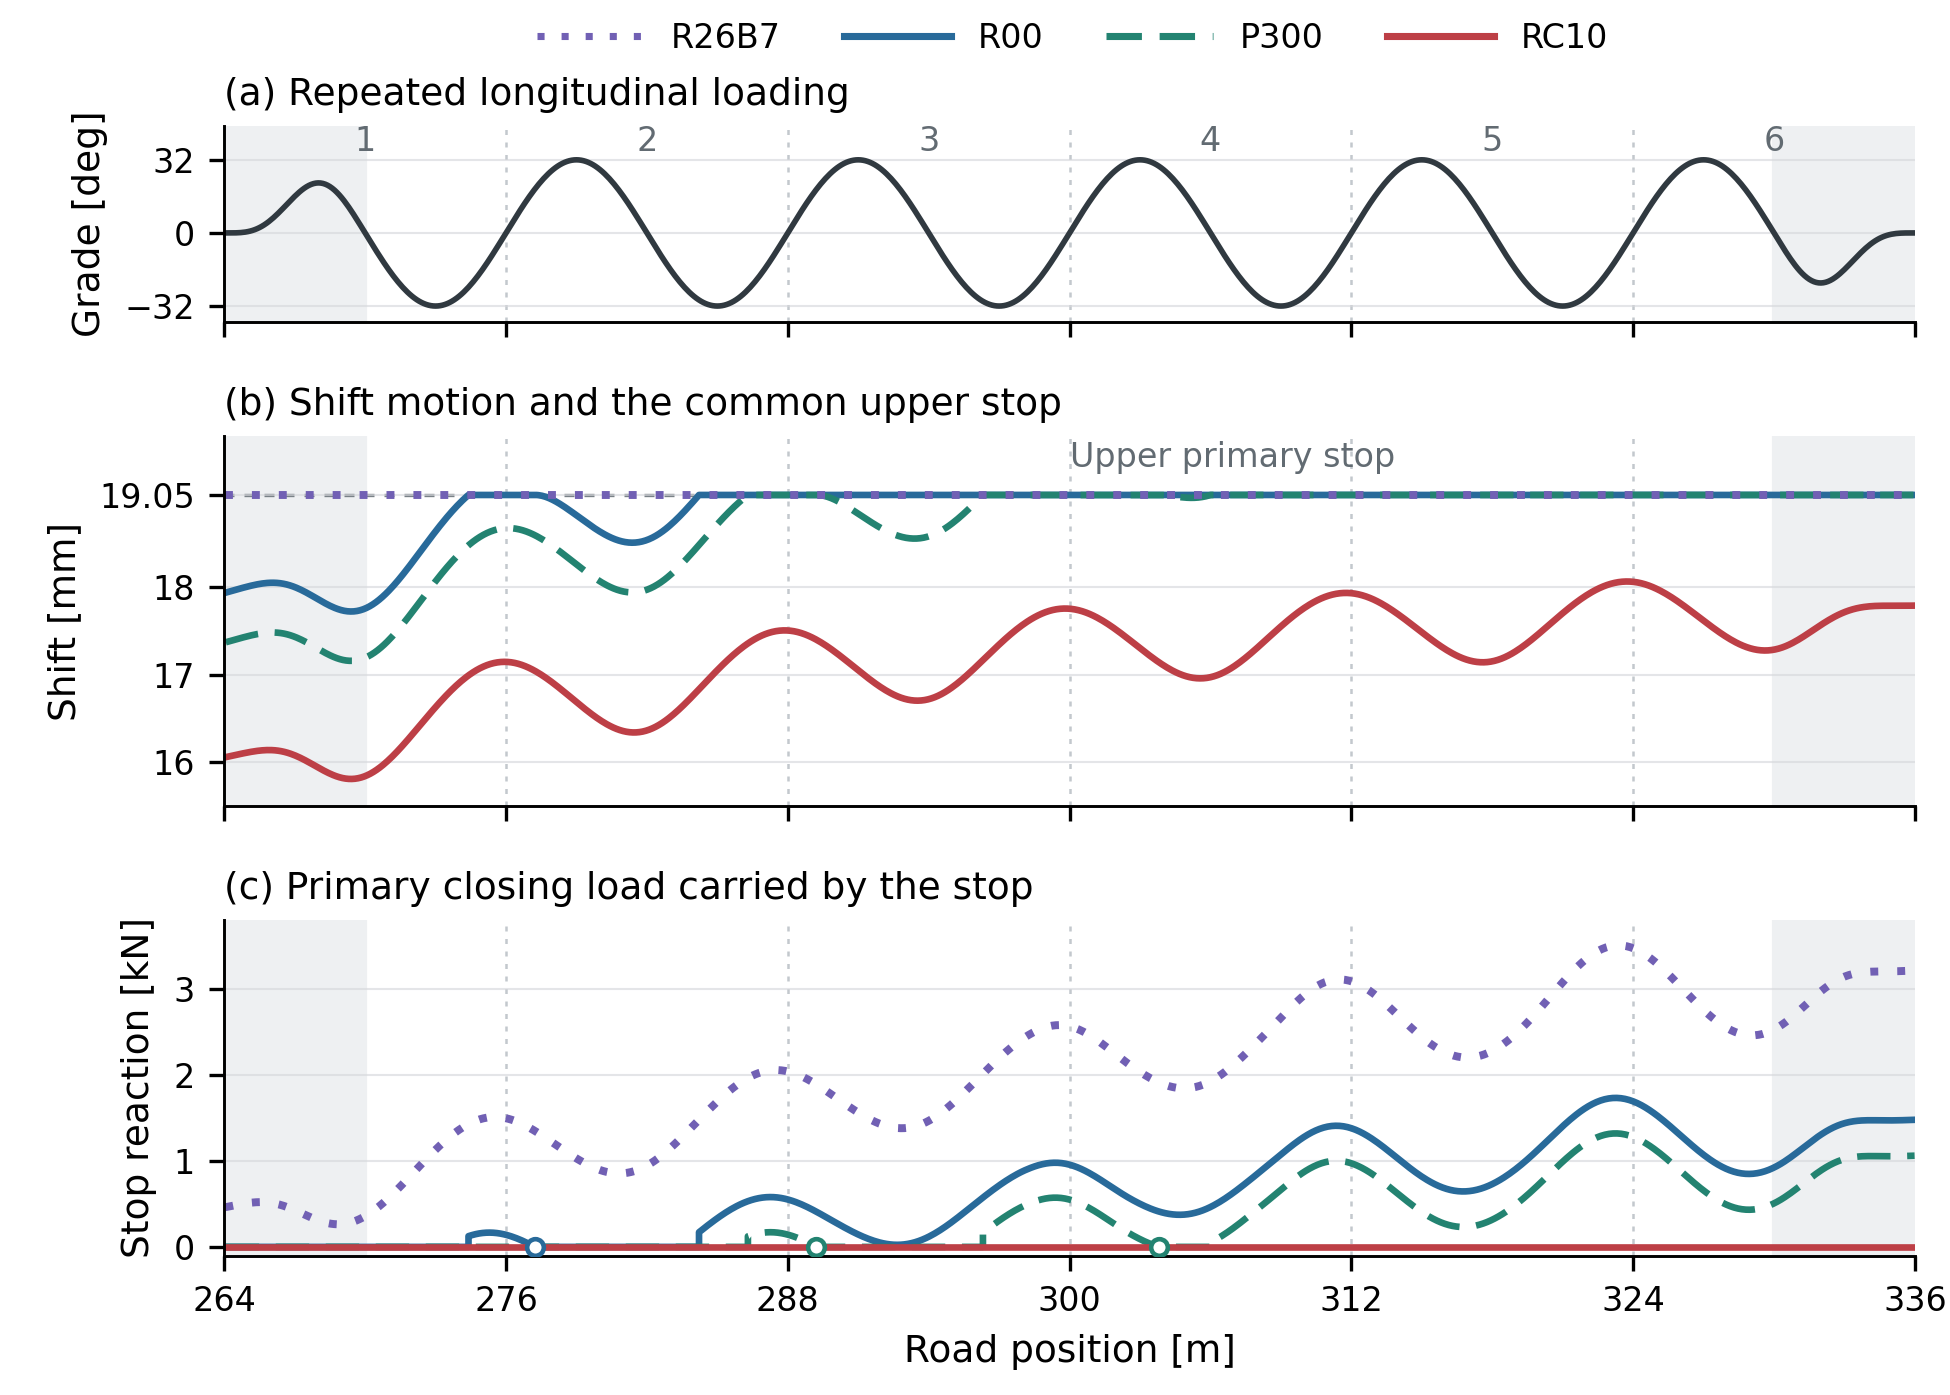
\includegraphics[width=\linewidth]{figures/results/course/cyclic_shift_and_support.png}
  \caption{Repeated loading from \SI{264}{m} to \SI{336}{m}. (a) Road grade,
  with cycles numbered and the \SI{6}{m} end tapers shaded; cycles 2--5 have
  the full \(\pm32^\circ\) amplitude throughout. (b) Shift position; supported
  traces coincide at the common upper stop. (c) Primary stop reaction, zero
  while the primary is away from the stop. Open circles mark recorded
  releases from support. Equal road position aligns the imposed grade, not
  elapsed time or the states inherited from the preceding road.}
  \label{fig:results_cyclic_support}
\end{figure}

R26B7 remains at the upper stop throughout all six cycles, but panel~(c)
shows that its loading is not constant. The stop carries the primary
closing force left after spring opposition and the belt's opening reaction
have been balanced. Its reaction varies with the drive yet remains positive,
so the primary stays pressed against the stop. This does not mean that
backshift has been mechanically blocked. The stop prevents further closure,
but cannot pull the primary closed: if holding that position would require
a tensile reaction, the primary must leave the stop and open.

R00 and P300 show that release directly. R00 reaches the stop during the
first cycle, reopens during the second, and then returns to remain supported
from the third cycle onward. With its greater spring opposition to closure,
P300 continues releasing during the third and fourth cycles. Its largest
backshift within a cycle falls from approximately
\SI{0.73}{mm} in cycle 2 to just \SI{0.03}{mm} in cycle 4; by cycle 5 it too
remains at the stop. The open circles in panel~(c) connect those departures
to the reaction falling to zero. Once the later load changes no longer
unload the stop, shift position stays fixed even though the grade continues
to vary. At that fixed geometry, the rising primary speed during continued
acceleration strengthens centrifugal closing, increasing the load available
to keep the primary pressed against the stop.

RC10's weaker late-travel centrifugal closing instead leaves the primary
below the upper stop throughout this region. Its shift continues to
rise overall, but each cycle still produces a distinct backshift: the
largest fall from an earlier shift maximum is approximately
\SI{0.81}{mm} in cycle 2 and \SI{0.79}{mm} in cycle 5. These opening
excursions distinguish the repeated response from the underlying upshift:
the primary continues to reopen appreciably even as its mean position moves
closer to the high-ratio limit.

Both belt contacts stick throughout this region in all four cases, so the
contrast is not caused by a loss of traction. Nor does the disappearing
shift oscillation in R00 and P300, by itself, establish damping: the reaction
and release history show how their motion gives way to sustained support.
Following the load carried by the stop makes that distinction visible even
when position alone becomes unchanging. The longer climb that follows asks
a different question: where the coupled transmission and engine operate
when the increased load is sustained rather than repeatedly reversed.

\subsection{Operating Conditions on a Sustained Grade}
\label{sec:results_moderate_hill}

The next climb holds the increased gravitational resistance long enough to
examine where the transmission operates after its initial backshift. The
road rises to \(18^\circ\) between \SI{348}{m} and \SI{356}{m}, then maintains
that grade for \SI{240}{m}. As before, backshift allows the vehicle to slow
without requiring the same reduction in engine speed. The useful comparison
is therefore not just how far the
CVT backshifts, but where that ratio places the engine and how much power it
can supply for the climb.

\Cref{fig:results_moderate_operating_conditions} follows the resulting
backshift and primary speed for R00 and five hardware variations. Each
trajectory retains the state inherited from the preceding road.
The adjoining engine characteristic relates the primary speed in panel~(b)
to the input power supplied for the climb.

\begin{figure}[H]
  \centering
  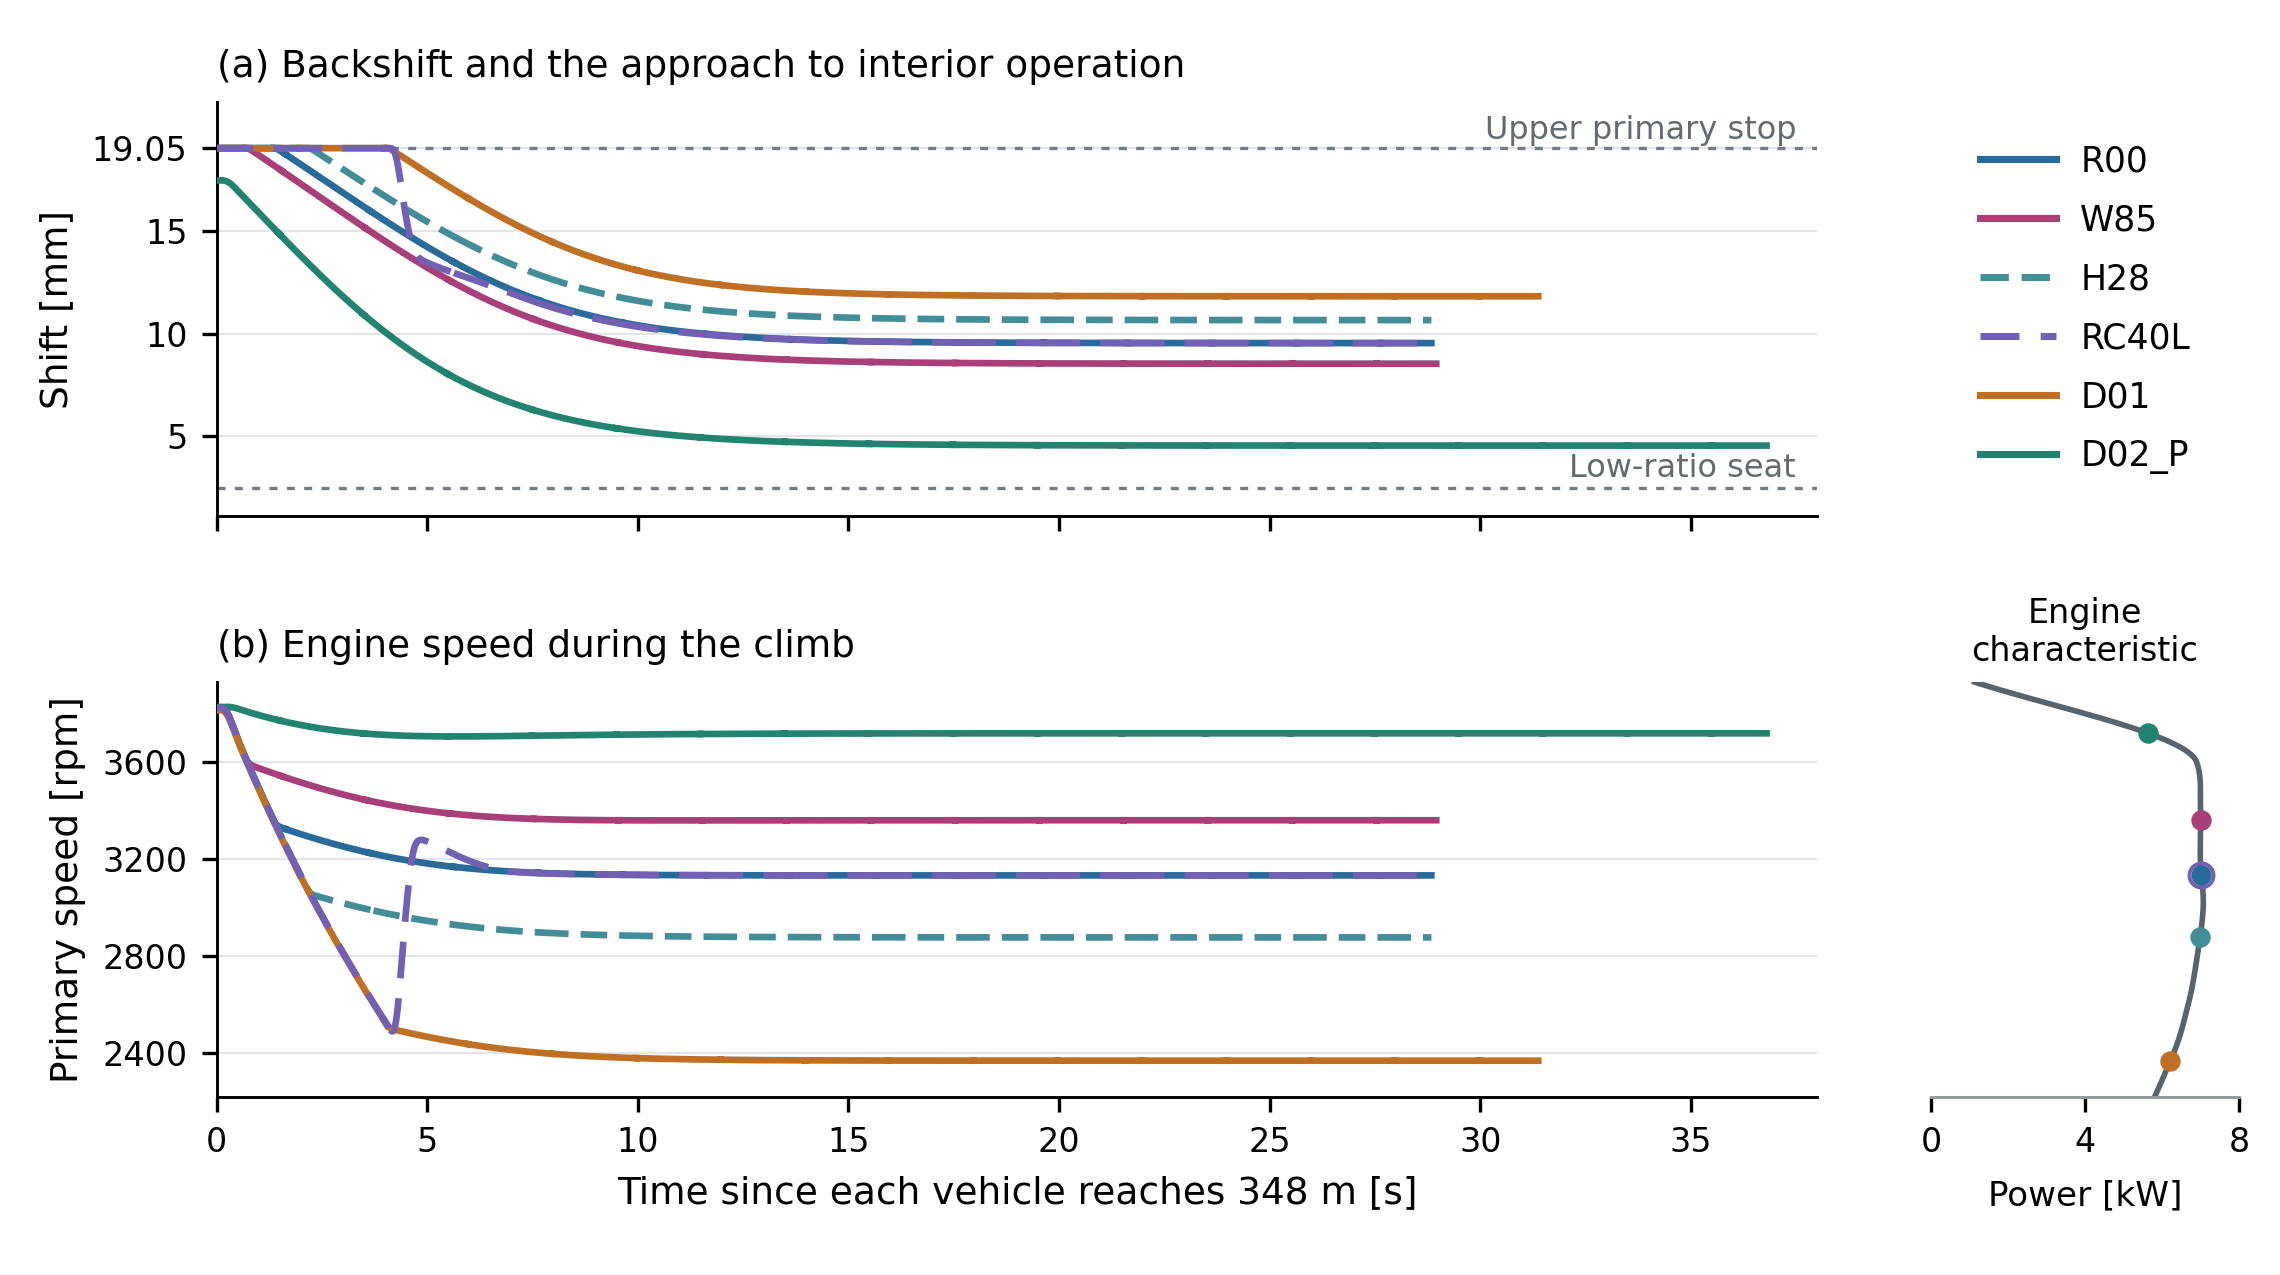
\includegraphics[width=\linewidth]{figures/results/course/moderate_hill_operating_conditions.png}
  \caption{Approach to sustained climbing on the \(18^\circ\) hill.
  (a) Shift position, with the common upper primary stop and low-ratio seat
  marked. (b) Primary speed. The engine-power curve on the right shares its
  speed scale, with coloured markers at the late mean primary speeds.
  Time is measured from each vehicle's arrival at
  \SI{348}{m}; each trace ends at \SI{596}{m}, before the grade decreases.
  Equal elapsed time does not imply equal road position. The later R00 and
  RC40L traces nearly coincide in both panels; their power-curve markers
  also overlap.}
  \label{fig:results_moderate_operating_conditions}
\end{figure}

R00 initially slows while still at the upper stop. Falling primary speed
weakens centrifugal closing until the primary can reopen under the
secondary's closing action. It then backshifts, limiting the further fall in
engine speed. The motion becomes small well before reaching the low-ratio
seat. Unlike the supported states in the preceding subsection, this nearly
fixed geometry is maintained within the available travel: primary
flyweight closing balances the spring and belt opening forces, while the
secondary spring and helix closing balance its belt reaction. Both balances
are satisfied without a stop reaction. The belt contacts remain
sticking throughout the displayed climb in all six cases.

RC40L takes a different path to almost the same final condition.
Its modified late ramp sustains primary closing farther into the hill,
delaying departure from the upper stop to about \SI{407}{m}, compared with
\SI{370}{m} for R00. Engine speed falls farther while the ratio stays fixed,
then recovers as the rapid backshift begins. At their common
later shift position of approximately \SI{9.55}{mm}, the roller contact lies
about \SI{15}{mm} along the physical ramp, within the first \SI{18}{mm} that
RC40L leaves unchanged. The altered ramp delays backshift, but the later
climbing geometry brings the roller back onto the reference profile and
leaves the local force balance almost unchanged.

The remaining cases show what happens when the hardware change continues to
affect that interior balance. \Cref{tab:results_moderate_operating_conditions}
pairs the late shift positions and engine speeds with vehicle speed and
engine input power. These quantities must be read together: once
acceleration becomes small, the engine must supply approximately the power
consumed by gravity, rolling resistance and aerodynamic drag at the
resulting climbing speed.

\begin{table}[H]
  \centering\small
  \setlength{\tabcolsep}{8pt}
  \renewcommand{\arraystretch}{1.14}
  \caption{Late operating conditions on the constant \(18^\circ\) grade.
  Values are time-weighted means over the final five-second window
  before \SI{596}{m}; all six cases have free shift and sticking contacts
  throughout these windows.}
  \label{tab:results_moderate_operating_conditions}
  \begin{tabular}{@{}lrrrr@{}}
    \toprule
    Case & Shift [mm] & Primary [rpm] & Speed [m/s] & Input power [kW] \\
    \midrule
    R00 & 9.55 & 3132 & 7.23 & 7.03 \\
    RC40L & 9.55 & 3132 & 7.23 & 7.03 \\
    W85 & 8.54 & 3360 & 7.20 & 7.00 \\
    H28 & 10.67 & 2877 & 7.19 & 6.99 \\
    D01 & 11.83 & 2368 & 6.42 & 6.22 \\
    D02\_P & 4.55 & 3719 & 5.85 & 5.64 \\
    \bottomrule
  \end{tabular}

\end{table}

W85 and H28 move to opposite sides of R00 in ratio and engine speed, yet
climb at almost the same vehicle speed. W85's lighter tips weaken primary
centrifugal closing at a given speed and geometry, allowing more backshift.
Its lower ratio keeps the engine turning faster for nearly the same output
speed. H28 changes the opposing side of this balance: its larger helix angle
reduces secondary axial closing for a given reacted torque, permitting
greater primary closure and a higher ratio. Its engine consequently turns
more slowly. Despite spanning approximately \(2877\)--\(3360~\mathrm{rpm}\),
these cases and R00 all operate in the nearly constant-power region of the
engine curve, at about \SI{7.0}{kW}. Their similar climbing speeds therefore coexist
with distinctly different internal ratios and shaft speeds.

Moving farther in either direction does not preserve that power. D01's
combined changes leave it farther upshifted, with the engine near
\(2368~\mathrm{rpm}\), supplying only \SI{6.22}{kW}. D02\_P retains the light
flyweights and backshifts much farther, raising engine speed to about
\(3719~\mathrm{rpm}\). At that speed the supplied engine characteristic is
already on its falling-power side, so the higher speed supplies only
\SI{5.64}{kW}. Their lower powers support lower climbing speeds of about
\SI{6.42}{m/s} and \SI{5.85}{m/s}, respectively, while both contacts still
stick. The difference is therefore attributable to where the coupled
mechanism places the engine, rather than to exhausted belt traction or a
travel stop. Additional backshift is useful when it preserves engine power;
beyond that, a lower ratio alone does not make the vehicle climb faster.

\subsection{Reverse Power on the Descent}
\label{sec:results_descent_reverse_power}

On the final \(-22^\circ\) descent, gravity can drive the vehicle and return
power through the CVT to the engine. Both shafts continue to turn forward;
the change is in which side drives the belt. \Cref{fig:results_descent_power}
follows R00 from the level approach through the descent and onto the final
level road. The two boundary powers use the same sign convention: positive
power adds energy to the corresponding shaft-side system, while negative
power removes it.

\begin{figure}[H]
  \centering
  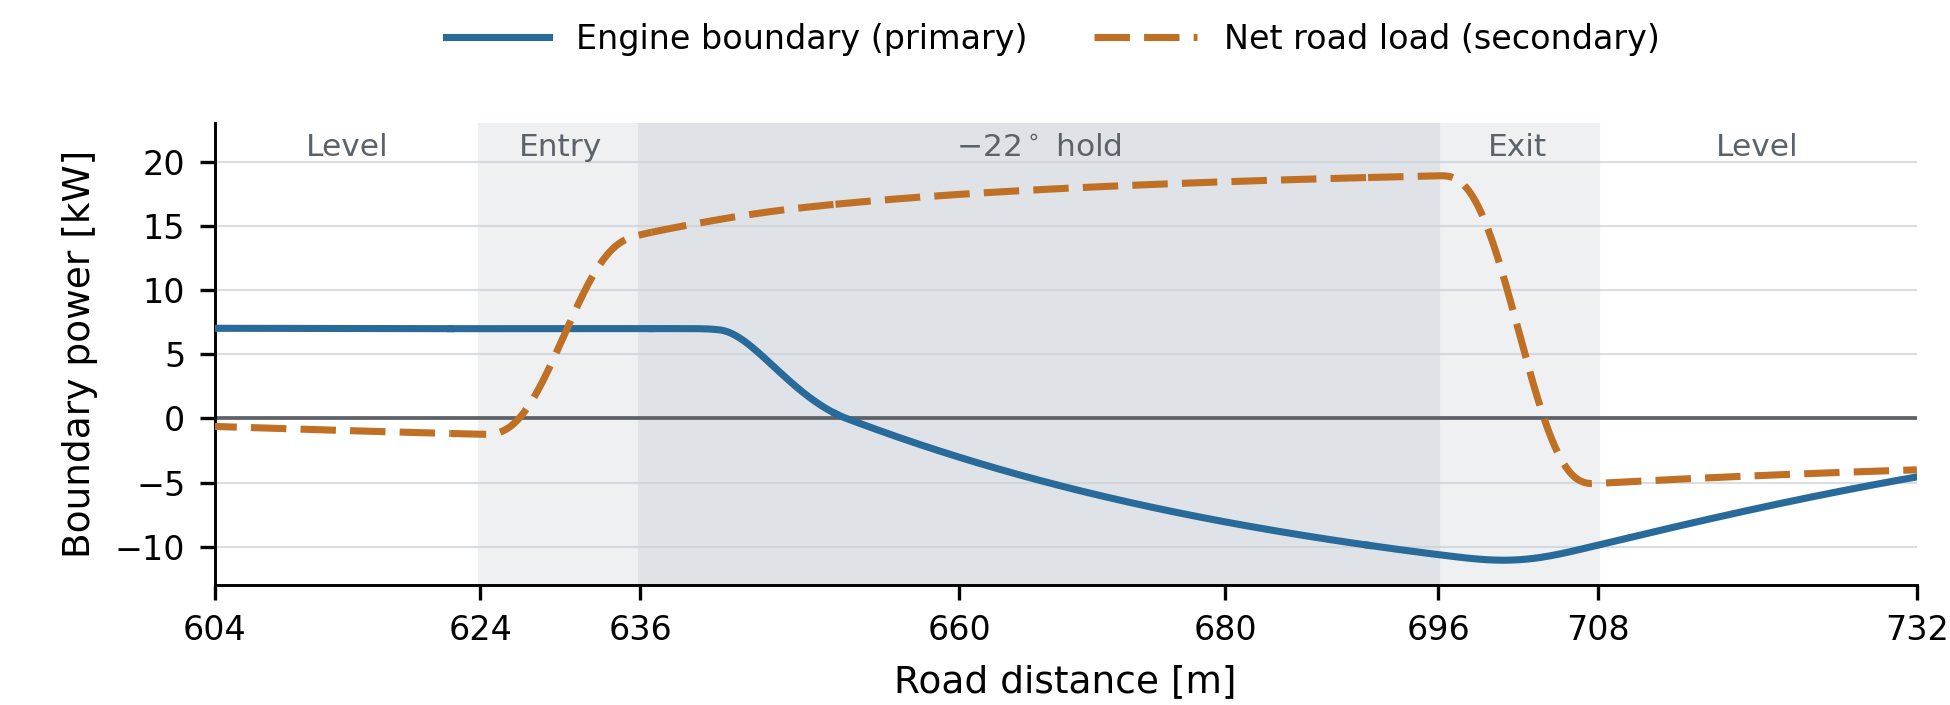
\includegraphics[width=\linewidth]{figures/results/course/descent_reverse_power.png}
  \caption{R00 boundary powers during the final descent.
  The primary trace is \(\tau_{\mathrm{B},p}\omega_p\); the secondary trace is
  \(\tau_{\mathrm{B},s}\omega_s\), equal to the net road force times vehicle
  speed. Grey shading marks the descent, with darker shading for the constant
  \(-22^\circ\) grade. Negative primary power denotes absorption by the engine
  boundary. These powers need not balance while the vehicle and transmission
  gain or lose kinetic energy.}
  \label{fig:results_descent_power}
\end{figure}

The road-side power becomes positive once gravity exceeds rolling resistance
and aerodynamic drag. Initially the engine still supplies power as well.
Near \SI{652}{m}, the primary passes \(4000~\mathrm{rpm}\), where the supplied
engine torque changes sign. The engine now absorbs part of the energy
supplied by the descent. The road supplies more power than the engine absorbs,
so the vehicle continues to accelerate
on the constant slope. The faster descent also releases more gravitational
energy each second. Over the speeds reached here, the increase in gravitational
power exceeds the increase in aerodynamic and rolling losses, so net road-side
power continues to rise. On the final level road, both boundary powers become
negative. The vehicle then slows, and its stored kinetic energy sustains the
remaining return of power to the engine.

This return path still requires sufficient belt clamping. R00 reaches the
upper primary stop near \SI{637}{m} and remains there, but fixing the pulley
geometry does not remove the traction limits. During reverse power, the belt
resists the secondary and drives the primary. Both contacts remain sticking:
over the descent entry, hold and exit, the primary uses at most about
\(0.19\) of its static capacity and the secondary about \(0.20\). The existing
clamping therefore carries the reversed torque with substantial capacity
remaining.

Full throttle remains prescribed throughout this calculation. The negative
engine torque comes from the extrapolated high-speed extension described in
\Cref{app:primary_engine_boundary}, not a measured closed-throttle CH440
braking characteristic. The absorption magnitude consequently depends on
that supplied boundary. The CVT carries this reverse power through the same
coupled shaft, belt and support mechanics used earlier for forward drive.

\subsection{What the Common Course Establishes}
\label{sec:results_course_synthesis}

The common course has shown the CVT responding as a complete dynamic
component between the engine and vehicle. Its motion and the internal
conditions needed to sustain it have been determined together as the
loading changes. Successful drive and loss of progress have therefore been
explained within the same formulation, through the forces carried by the
hardware and the limits of its contacts and supports.

The sheaves that squeeze the belt also set its running radii, so the
actuation responsible for grip participates in changing or holding the
ratio. While both contacts stick, that ratio links engine and vehicle
speeds. The resulting shaft speeds and transmitted torque influence primary
centrifugal and secondary helix action, while sheave motion changes spring
loading and actuator geometry. A hardware change therefore alters the
forces and the operating conditions under which those forces are produced.

A tune must consequently be judged by the loaded drive it produces.
Enough traction and a ratio that makes useful engine power available have
to be achieved by the same hardware as it responds to changing loads.
Within the adopted component and boundary laws, the formulation makes that
connection traceable. A vehicle response can be followed back to the forces
and constraints that produced it, and a proposed hardware change can be
followed forward through the operating conditions it creates.

\chapter{Conclusion and Future Work}
\label{sec:conclusion_and_future_work}

\section{Conclusion}
\label{sec:conclusion}

TODO

\section{Future Work}
\label{sec:future_work}

The present formulation follows how the shafts, actuators, and belt respond
together as the CVT changes operating condition. Its assumptions also identify
where that description can be extended. Some omitted forces can be added to
the existing free bodies; other changes would let the belt move and deform in
ways that its present coordinates cannot describe. The extensions below
examine how those effects change the transient response.

Much of the local physics needed for these extensions is already described in
the literature reviewed in \Cref{sec:literature-review}. Adding those
mechanisms must preserve the way the belt, pulleys, and actuators respond to
one another over time. Some descriptions assume steady running, prescribe part
of the motion, or determine a component's position through instantaneous force
balance. Where these restrictions remove an interaction needed here, the local
relations must be reconsidered and coupled to the equations of motion. Belt
loading must affect how the hardware accelerates, while that motion changes
the contact conditions and loading in return.

\subsection*{Actuator Friction and Directional Shifting}
\label{sec:future_work_mechanism_friction}

The actuator mechanisms can also resist motion in a direction-dependent way.
The same mechanism position therefore need not produce the same clamping force
while the CVT shifts in opposite directions. Acceleration can already
contribute to this distinction in the present model because part of the applied
loading accelerates the actuator itself. Friction in the ramps, helix, and guides
would add resistance that changes direction with the relative motion. Static
friction could also delay the start of motion or hold a sheave away from a
travel stop. These effects are excluded by
\AssRef{assump:ideal_actuator_mechanics}; their forces would enter the primary
free body and secondary helix balance in
\Cref{eq:primary_movable_sheave_balance,eq:secondary_reacted_helix_torque_structure}.

In his tuning handbook, \citet{Aaen2007} describes how reversal of friction at
the secondary cam and sliding buttons delays backshift and allows engine speed
to fall. \citet{KimEtAl2002} include friction in their mechanical-actuator
relations, while \citet{Cammalleri2005} distinguishes its direction at the
start of upshift and downshift. Adding these forces to the dynamic balances
would let us examine how much actuator friction contributes to the difference
between upshift and backshift curves during complete maneuvers, including how
engine speed recovers after a load increase.

That difference also depends on belt contact and inertia. Comparisons at
different shift rates, with actuator friction characterised independently,
could help distinguish these causes of delayed reversal. For the roller
mechanisms considered here, the relevant resistance may come from roller
bearings and rolling contact rather than the sliding buttons discussed by
Aaen. In either case, friction changes the contact reaction that generates the
clamping force, so it must be included in the actuator balance.

\subsection*{Face Torque and Dynamic Helix Response}
\label{sec:future_work_face_torque}

The secondary actuator also depends on how belt torque is divided between its
two sheave faces. The movable face rotates relative to the shaft as it shifts,
so the belt generally encounters a different surface velocity on each face.
The current formulation includes this relative rotation in the actuator and
shaft dynamics and uses the power-equivalent contact speed in
\Cref{eq:representative_contact_angular_speed}. What it does not determine is
the division of torque between the two contacts:
\AssRef{assump:symmetric_face_sharing} supplies \(\tau_{s,M}=\tau_s/2\) in
\Cref{eq:secondary_movable_face_belt_torque}.

\citet{SorgeCammalleri2011} show why this division deserves closer attention.
Their separate face-contact calculations produce substantially unequal
torques, with circumferential tractions that can oppose one another over parts
of the wrap. In some calculated conditions, even the total torque on the
faster half-pulley is negative. Their analysis accounts for how relative face
motion changes contact while neglecting inertia other than centrifugal
loading. The present formulation includes the torque needed to accelerate the
movable assembly but uses the prescribed equal share for the two face
contacts. The two descriptions address different consequences of the same
motion.

\Cref{eq:secondary_reacted_helix_torque_structure} shows how the face torque
enters the helix balance. The helix reacts the belt and spring torques
remaining after the movable assembly has been accelerated. Replacing the
prescribed half-share by the calculated movable-face torque changes that
reaction and hence the axial force in \Cref{eq:secondary_helix_closing_force}.
The changed acceleration alters the relative face motion, which changes the
contact conditions that supplied the torque. The shaft balance responds at the
same time. Contact power would also be calculated from each face's torque and
speed, replacing the equal-share reduction in
\Cref{eq:secondary_face_tangential_power}.

The changes in shift motion found in \Cref{sec:results_secondary_helix} make
this coupling worth investigating during smooth shifting, rapid backshift, and
torque reversal. Comparing separate face contacts with and without the helix
dynamics would show whether their interaction changes sheave motion or the
approach to a contact or support transition. The separate torques and helix
reaction could show changes that are not visible in total transmitted torque
alone. This would help determine when the equal-share approximation is
sufficient for predicting the shift response.

\subsection*{Secondary Contact and Clearance}
\label{sec:future_work_secondary_contact}

The helix reaction also raises a question about the contact that carries it.
The reference mechanism uses a slot with no clearance, so either flank can
carry the helix reaction (\Cref{app:reference_helix_topology}). When the
reaction changes direction, the load transfers immediately to the opposite
flank. A one-sided helix could instead separate, while finite clearance in a
slot would allow relative motion before the opposite flank is reached.
Comparing these arrangements under the reaction reversals in
\Cref{sec:results_secondary_hybrid_response} would show how clearance or
separation changes the response.

While flank contact is absent, the movable assembly's rotation and axial
motion would no longer be linked by the helix geometry. Allowing those motions
to evolve independently would determine when contact returns and how clamp
develops during the interval. The model would need to allow that extra motion;
adding friction to the existing balance would leave the helix constraint in
place. The opening of a helix contact remains distinct from belt lift-off,
which depends on the normal loading at the belt--sheave interface.

\subsection*{Belt Deformation, Transport, and Contact}
\label{sec:future_work_belt_material}

Beyond the actuator mechanisms, the belt itself can be given more freedom to
move and deform. In the present formulation, it couples the two pulleys through
a fixed length, a single transport speed, and prescribed section geometry.
With the fixed length of \AssRef{assump:constant_belt_length}, the compatibility
relation in \Cref{eq:belt_length_compatibility} determines the secondary
position from the shared shift coordinate. The belt could instead stretch to
take up part of a sheave displacement. Tension would then depend on how much
the belt stretches, and \Cref{eq:secondary_coordinate_map} would no longer
determine the secondary position from the primary position alone. Each movable
sheave may then need its own position coordinate and equation of motion.

The dynamic belt model of \citet{Ballew2015} provides a starting point for
examining this coupling. It already calculates belt-node motion and both
pulley speeds together, but its running-radius search matches belt axial
reaction to applied clamp without calculating the movable sheave's axial
acceleration from its own force balance. Adding that balance would let sheave
and actuator inertia affect the response. Such a comparison could help explain
the different clamp-to-shift responses identified in
\Cref{sec:results_ballew_interpretation}.

\AssRef{assump:single_belt_speed} gives the whole loop one tangential
transport speed. Allowing that speed to vary from place to place would add
motion that need not come from belt stretch:
\citet{CarboneMangialardiMantriota2005} already describe local speed changes
caused by changing geometry in a belt that does not stretch. Following this
motion over time would require reconsidering the steady path and constant mass
flow assumed by \citet{Messick2018}.

Those speed differences also change how contact can be determined. A single
belt--pulley speed difference would no longer generally describe relative
motion throughout the wrap. The present equations describe how tension and
normal loading vary, but \AssRef{assump:wrap_contact_resolution} assigns one
contact state and one traction utilisation \(\lambda_j\) to each wrap through
\Cref{eq:lambda_local_definition}. Different motions along the wrap could
produce adhering and sliding regions, or regions with opposing traction,
within the same wrap. A local Coulomb law could still represent friction, with
contact states and traction determined along the wrap rather than assigned to
it as a whole.

The relative velocity must be calculated between the contacting rubber and the
sheave surface. Under \AssRef{assump:fixed-belt-cross-section}, the section
geometry and cord location are prescribed. Compression and bulging would
change belt width and contact shape, altering the relation between sheave
position and running radius. Shear and warping allow the rubber between the
tension-carrying layer and the sheave to deform. As \citet{Gerbert1996} shows,
the cord and pulley can then have different speeds while the rubber surface
adheres. Bending stiffness also affects seating and unseating as the belt
enters and leaves a wrap; Gerbert shows that these processes can produce
friction opposing the main torque-transmitting direction at the primary.

Sectional analysis offers a way to retain these effects without representing
every cord or cog around the loop. \citet{Gerbert1996} uses it to construct an
effective shear relation. Similar reductions could supply sectional forces,
moments, and deformed contact geometry to the belt model. If a section adjusts
much faster than the overall belt motion, the inertia of its internal motion
may be negligible even though its deformation changes contact. Representing
the distribution of cord and rubber mass more accurately could also improve
the inertia calculation without resolving every local deformation.

Under \AssRef{assump:gross_coulomb_traction}, friction acts only in the
circumferential direction, leaving out resistance to radial migration.
Traction along a sheave face can have both radial and circumferential
components. Resistance to changing running radius and resistance to tangential
slip therefore share the available contact traction.
\citet[p.~645]{KimEtAl2002} use this connection to explain the different
coefficients in their experimentally identified upshift and downshift laws.
Their proposed pseudo-self-locking mechanism occurs at the primary
belt--groove interface: outward radial friction during downshift can support a
condition resembling steady running, whereas its reversal during upshift
changes the radial and circumferential sliding. This supplies a belt-contact
contribution to directional shifting alongside actuator friction.

The groove-contact model of \citet{KongParker2006} and shifting analysis of
\citet{Sorge2008} provide ways to calculate friction direction from local
relative motion. Using these forces in the belt and sheave balances would show
how radial resistance, torque transmission, and axial thrust develop together
during shifting. A friction coefficient that varies with pressure or sliding
speed would provide a further extension. Its effect on available traction
could also be examined using the present belt coordinates.

These deformations and contact motions also change how mechanical work is
stored and dissipated. Elasticity stores and returns energy; viscoelasticity
adds dependence on deformation history and can dissipate energy during
repeated stretching, compression, shear, and bending. Surface sliding
dissipates work at the belt--sheave interface. The entry and exit processes
considered by \citet{Bertini2014} recur as the belt circulates, so their
contribution to loss continues after initial clutching. Messick measures
temperature- and frequency-dependent rubber properties but uses an elastic
approximation in the mechanical model; Ballew identifies independent damping
measurements as unfinished work \citep{Messick2018,Ballew2015}. A material law
for this motion would need the deformation history of each belt section as it
passes through the spans and wraps. Adding stored strain energy and material
dissipation to the energy balance in \Cref{eq:verification_energy_balance}
would show how much of a drop in output power comes from energy being stored
in the belt and how much is lost through sliding and material damping.

With compliance and inertia included, changes in tension and deformation could
travel around the loop after a sudden load change. \citet{Messick2018}
identifies engine torque that varies with crankshaft angle as a possible
source of vibration outside the scope of his steady model. A transient belt
model could show how strongly these torque fluctuations affect contact loading
and traction. Repeating the calculation with finer resolution along the belt
and smaller time steps would help distinguish physical vibration from
numerical oscillation, particularly given the stiffness difficulties reported
by \citet{Ballew2015}.

\subsection*{Belt Path, Support, and Re-engagement}
\label{sec:future_work_belt_path}

The above belt motions can still be described while the loop remains on the
prescribed circular wraps and straight spans. Relaxing the path itself is a
separate extension. The circular wraps and straight spans of
\AssRef{assump:prescribed_belt_path} remove possible motions before the force
balances are solved. The checks in
\Cref{eq:wrap_contact_admissibility} can identify a negative tension or local
normal load. They cannot determine the shape of a slack belt or one that has
partly lifted away from a pulley. Solving for the belt's shape and where it
contacts the pulleys would allow the model to follow what happens next.

This would be especially useful while the primary is disengaged. Under
\AssRef{assump:deadzone_belt_closure}, the belt is carried without slip by the
fully closed secondary through \Cref{eq:deadzone_secondary_lock}. A belt with
its own deformation and contact motion could instead determine installed
pretension, slack take-up, support at the primary hub, intermittent sheave
contact, and possible secondary slip. Initial engagement would then depend on
the belt's shape and motion at that time. These are changes to the physical
description of engagement, beyond refining its event time.

Existing models already solve for belt paths and contact boundaries
\citep{KongParker2005,KongParker2006,JulioPlante2011}. The question here is
how the belt and actuators respond to one another during disengagement and
re-engagement when the belt is free to leave the prescribed path. The
difficulty reported by \citet{JulioPlante2011} in obtaining stable results
near the clutching-to-shifting transition makes low-load engagement a
particularly useful test.

Planar motion may be sufficient for some studies of tension redistribution and
slackness. Axial migration, skew, and section twist require out-of-plane
motion. A floating secondary can also move along its shaft as a whole,
separately from opening its groove. Pulley compliance and shaft misalignment
are separate extensions of \AssRef{assump:rigid_hardware} and
\AssRef{assump:axis_alignment}. The metal-belt and chain-CVT studies of
\citet{CarboneMangialardiMantriota2005} and \citet{DuanEtAl2016} show that
hardware deformation can alter contact. For the loads considered here, its
effect would need to be compared with that of rubber deformation.

\subsection*{Friction and Compliance During Finite-Speed Events}
\label{sec:future_work_events}

The extensions above concern how the CVT moves while its active constraints
remain unchanged. Once engagement or a travel stop creates a new constraint at
finite relative speed, the event itself introduces a different set of contact
questions. The impulse--momentum balance in
\Cref{eq:finite_event_generalized_impulse_momentum} determines the resulting
velocity change. This treatment allows the simulation to continue through the
event. Two extensions would examine which contact details can change its
outcome.

The first concerns friction during the instantaneous event. Under
\AssRef{assump:impact_tangential_contact}, an existing sticking belt contact
transmits the impulse required to remain stuck without a separate friction
capacity check. A friction law relating tangential and normal impulses could
determine whether sticking can be maintained or the event produces tangential
slip. The constraints immediately after the event in
\Cref{eq:finite_event_outgoing_constraints} would then depend on the contact
impulses allowed by that law, following the frictional-impact framework
discussed by \citet{Stewart2000RigidImpact}.

The second concerns contact duration. The instantaneous, perfectly inelastic
treatment in \AssRef{assump:inelastic_constraint_activation} determines the
motion and energy change across the event, but cannot resolve peak force,
rebound, or vibration during capture. Following contact deformation over time
would allow the model to calculate these forces and motions. Friction-limited
impulses and finite-duration contact therefore answer different questions:
whether the contact can remain stuck after the event, and how much contact
deformation and duration change the response. The instantaneous description
may remain sufficient for the overall shift motion even where resolving peak
loads requires compliance.

\subsection*{Temperature During Transient Operation}
\label{sec:future_work_temperature}

The losses in the belt and its contacts can also change the properties that
determine the motion that follows. Under
\AssRef{assump:material_surface_state}, those properties remain fixed
throughout a run. The measurements of \citet{Messick2018} show that rubber
stiffness and dissipation depend on temperature and loading frequency. The
same maneuver may therefore produce a different response from a cold or warm
belt. The question is whether fixed properties at the measured initial
temperature are sufficient, or whether heating during the maneuver changes the
mechanics enough that the model must follow temperature as it changes.

The temperature of the belt as a whole is only part of the question. Local
contact can heat over much shorter distances and times than the bulk material.
\citet{Persson2006FlashTemperature} describes how flash heating feeds back
into rubber friction through the temperature-dependent material response. In a
CVT, heat generated during clutching or brief slip may change the friction
available as traction recovers. Its importance at the belt--sheave interface
remains to be established. A nearly unchanged bulk temperature during a short
maneuver would not, by itself, show that flash heating is negligible.

\subsection*{Experimental Validation and Characterisation}
\label{sec:future_work_validation}

These extensions also require experiments that can separate the effects they
are intended to represent. Different operating conditions allow different
parts of the model to be tested. While a travel stop holds the sheaves in place, loading can be varied
without changing the pulley geometry. Free shifting then allows the
predicted sheave motion to be tested. A travel stop also carries a reaction:
the belt load need not equal the actuator force because the stop carries the
remainder of the axial balance. \citet{GrzegozekDobajKot2016} identify this
limitation when inferring belt loads from regulator characteristics. The
reactions in \Cref{tab:structural_stop_reactions} therefore require
measurements beyond the actuator law if supported operation is to test the
predicted belt loading.

Measurements during shifting should also include more than shaft speeds. In
the model comparison of \Cref{sec:results_ballew_closed_loop}, feedback brings
the shaft speeds close to the reference traces while producing a substantially
different primary clamp. Applying the reference force directly in
\Cref{sec:results_ballew_force_replay} removes the feedback adjustment and
gives a different response. Sheave displacement distinguishes geometric
shifting from the speed changes produced by slip; belt speed, torque, and
selected actuator loads can further distinguish the causes.
\citet{Bertini2014} measure both thrust and torque in their tests. For the
secondary face-torque coupling, movable-face torque or helix reaction would be
more informative than total shaft torque alone. If a measured force is
supplied as an input, agreement in that force does not test the model's
ability to predict it.

The shaft boundaries defined in \Cref{sec:system_definition} allow these
comparisons to use a wide range of test arrangements. An engine or motor can
drive the primary, while a brake, rotating inertia, or attached drivetrain
loads the secondary. Their influence enters through the shaft interface in
\Cref{eq:shaft_boundary_interface}, so changing the apparatus need not change
the internal CVT formulation. With the applied loading and initial state
specified, measurements can test predicted shaft and sheave motion through
engagement, acceleration, upshift, backshift, and traction recovery. Different
arrangements allow different loads and measurements, so the predictions that
can be tested depend on what the rig applies and independently measures.

Material and component properties also need independent measurements.
Geometry, inertia, and spring characteristics establish the mechanical inputs.
Actuator friction requires measurements through holding, breakaway, and
reversal, while belt tests must distinguish elastic storage from dissipation
under relevant stretching, compression, shear, and bending. The tests
described by \citet{Ballew2015} and \citet{Messick2018} provide foundations,
with further work needed on damping and dependence on loading history.
Belt--sheave friction also requires independent characterisation over the
relevant loads, speeds, and temperatures. These
measurements would allow complete-CVT experiments to test how the belt,
pulleys, and actuators respond together without adjusting the physical
parameters to match each maneuver.

\subsection*{Recovery and Assessment of the Reduced Model}
\label{sec:future_work_reductions_design}

The present formulation can serve as a common reference for these extensions.
Wherever a reduction is well defined, applying the same assumptions and
closure relations again should lead back to the equations used here. The
reduced model should then reproduce the same response, within numerical
accuracy, under corresponding loading and initial conditions.

With the added mechanisms active, the next question is how much they change
the response. The comparisons in \Cref{sec:results_reduced_belt_mechanics}
show why the equations need to be solved again: a term's size in one run does
not tell us how much the motion changes when that term is removed. Changes in
clamp demand, shift timing, traction recovery, or contact transitions would
show which predictions depend on the added mechanics. Experiments could then
test whether the new predictions agree more closely with measurements. If the
added mechanisms make little difference to the predictions needed for a
component or design study, the simpler model may be enough. Each extension
could then help show which questions the present formulation can answer and
which need more detail.

\section*{Author Contributions (CRediT)}

\noindent\textbf{Kai Arseneau:} Conceptualization; Methodology; Software;
Formal analysis; Visualization; Writing~--~original draft;
Writing~--~review \& editing.

\noindent\textbf{W.~Spencer Smith:} Supervision;
Writing~--~review \& editing.

\bibliographystyle{plainnat}
\bibliography{../../refs/References,CINDER_Appendix_References}

\appendix

\chapter{Construction of Primary Flyweight Geometry Maps}
\label{app:primary_flyweight_geometry}

The primary actuator dynamics derived in the main text do not require a particular
flyweight shape directly. They require the mechanism maps
\begin{equation}
    q_f=q_f(x_p),
    \qquad
    \frac{dq_f}{dx_p},
    \qquad
    \frac{d^2q_f}{dx_p^2},
    \qquad
    J_{f,p}=J_{f,p}(x_p),
    \qquad
    \frac{dJ_{f,p}}{dx_p},
    \label{eq:appB_required_maps}
\end{equation}
together with the constant pivot-axis inertia \(I_f\). This appendix constructs
those quantities for the fixed-pivot roller flyweight used by the present
primary mechanism.

The construction follows the physical mechanism directly. A ramp attached to
the movable sheave defines the contact surface. The finite roller radius offsets
that surface to a roller-centre locus. Intersecting that locus with the rigid
flyweight-arm circle determines the assembled flyweight pose and therefore
\(q_f(x_p)\). Differentiating the same geometric constraint supplies the motion
ratios required by the acceleration-level actuator model. Finally, the
flyweight mass distribution is evaluated at the resulting pose to obtain
\(I_f\), \(J_{f,p}(x_p)\), and \(dJ_{f,p}/dx_p\).

No independent initial flyweight angle is introduced. The assembled pose is a
consequence of the pivot, ramp, roller, and arm geometry.

% ==============================================================
\section{Fixed-Pivot Flyweight Geometry}
\label{app:flyweight_pivoted_roller}
\label{sec:primary_flyweight_geometry_examples}

Consider the axial--radial plane of one primary flyweight. Let \(O\) denote the
shaft centre, let \(+\bm e_x\) point in the positive primary closing direction,
and let \(+\bm e_r\) point radially outward. The flyweight pivots about the
fixed point
\begin{equation}
    \bm r_P
    =
    \begin{bmatrix}
        x_P\\
        r_P
    \end{bmatrix},
\end{equation}
which is fixed to the pulley body. The movable sheave carries the physical ramp.
The roller centre is denoted by \(C\), the physical roller--ramp contact point
by \(K\), and the reference point at the start of the active ramp by \(A\).

The rigid distance from the pivot to the roller centre is
\begin{equation}
    \boxed{L_f=|PC|},
    \label{eq:appB_arm_length}
\end{equation}
and the roller radius is \(R_{\mathrm{roll}}\). The flyweight angle \(q_f\) is
measured from the positive axial reference to the line from \(P\) to \(C\),
with increasing \(q_f\) corresponding to outward flyweight rotation. Thus
\begin{equation}
    \bm r_C(q_f)
    =
    \bm r_P
    +
    L_f
    \begin{bmatrix}
        \cos q_f\\
        \sin q_f
    \end{bmatrix}.
    \label{eq:appB_roller_center_from_q}
\end{equation}
The arm is therefore constrained to a circle of radius \(L_f\) about \(P\).

\subsection{Physical Ramp Representation}
\label{app:flyweight_general_ramp}

Introduce a scalar ramp coordinate \(\xi\), with \(A\) corresponding to
\(\xi=0\). Let \(h(\xi)\) be the radial profile measured from \(A\), and let
\(d_x\in\{-1,+1\}\) specify whether increasing \(\xi\) proceeds in the positive
or negative physical axial direction. For movable-sheave closure \(x_p\), a
point on the physical ramp is
\begin{equation}
    \boxed{
    \bm r_K(\xi,x_p)
    =
    \begin{bmatrix}
        x_A+x_p+d_x\xi\\[2mm]
        r_A+h(\xi)
    \end{bmatrix}.
    }
    \label{eq:appB_ramp_global}
\end{equation}
The present Baja parameterization uses \(d_x=-1\): increasing profile
coordinate proceeds axially toward the pivot while the ramp rises radially
outward.

Ramp angle is measured from the axial reference line, so \(0^\circ\) denotes an
axial ramp. For a graph of the form in \Cref{eq:appB_ramp_global}, the local
unsigned ramp angle satisfies
\begin{equation}
    \alpha(\xi)=\tan^{-1}|h'(\xi)|.
\end{equation}
Accordingly, a \(20^\circ\) ramp is nearly axial rather than nearly radial.

The unnormalized tangent is
\begin{equation}
    \bm t(\xi)
    =
    \begin{bmatrix}
        d_x\\
        h'(\xi)
    \end{bmatrix},
    \qquad
    \|\bm t\|=\sqrt{1+[h'(\xi)]^2}.
    \label{eq:appB_ramp_tangent}
\end{equation}
With \(\sigma_n\in\{-1,+1\}\) selecting the physical side of the ramp on which
the roller lies, a compatible unit normal is
\begin{equation}
    \boxed{
    \bm n(\xi)
    =
    \sigma_n
    \frac{
        \begin{bmatrix}
            -h'(\xi)\\
            d_x
        \end{bmatrix}
    }{
        \sqrt{1+[h'(\xi)]^2}
    }.
    }
    \label{eq:appB_ramp_normal}
\end{equation}
The sign \(\sigma_n\) is fixed once from the assembled mechanism and is then
used throughout the active ramp range.

The profile \(h\) may be assembled from straight, circular, spline, or other
smooth segments. Those shapes define only the physical contact surface; they do
not themselves prescribe the flyweight motion or force.

\subsection{Finite-Radius Roller-Centre Locus}
\label{app:flyweight_offset_curve}

The roller centre does not lie on the physical ramp. At contact it is offset by
one roller radius along the selected ramp normal:
\begin{equation}
    \boxed{
    \bm r_C(\xi,x_p)
    =
    \bm r_K(\xi,x_p)
    +
    R_{\mathrm{roll}}\bm n(\xi).
    }
    \label{eq:appB_offset_curve}
\end{equation}
This finite-radius offset is the roller-centre path used by the mechanism. The
point \(K\) remains the physical contact point; \(C\) is the centre of the
roller bearing.

The contact problem can now be viewed geometrically as the intersection of the
roller-centre offset curve with the rigid circle of radius \(L_f\) about \(P\).
A point-contact or zero-radius follower approximation is not used for the
present mechanism.

\subsection{Rigid-Arm Contact Constraint and Assembled Branch}
\label{app:flyweight_solve_q}

A roller-centre location is compatible with the rigid flyweight when
\begin{equation}
    \boxed{
    g(\xi,x_p)
    =
    \left\|
        \bm r_C(\xi,x_p)-\bm r_P
    \right\|^2
    -
    L_f^2
    =0.
    }
    \label{eq:appB_contact_residual}
\end{equation}
For any fixed \(x_p\), every root of \Cref{eq:appB_contact_residual} is a
mathematical flyweight configuration that satisfies the rigid arm and roller
contact geometry.

Define
\begin{equation}
    a=x_C-x_P,
    \qquad
    b=r_C-r_P.
    \label{eq:appB_ab_def}
\end{equation}
Then
\begin{equation}
    a^2+b^2=L_f^2,
\end{equation}
and the corresponding flyweight angle is
\begin{equation}
    \boxed{
    q_f(x_p)=\operatorname{atan2}(b,a).
    }
    \label{eq:appB_q_map}
\end{equation}
Thus the starting angle is recovered from the assembled geometry rather than
specified as an independent parameter.

Multiple mathematical roots can exist at the same \(x_p\). At the beginning of
the declared operating interval, \(x_p=x_{p,\min}\), enumerate the admissible
contact configurations and initialize the assembled branch with
\begin{equation}
    \boxed{
    q_f(x_{p,\min})
    =
    \min_i q_{f,i}(x_{p,\min}).
    }
    \label{eq:appB_initial_branch_rule}
\end{equation}
This smallest-\(q_f\) rule is an \emph{initial assembly rule only}. For increasing
or decreasing closure thereafter, the same solution branch is followed
continuously. The flyweight is not permitted to jump to a disconnected arm
orientation simply because another root has a smaller angle at a later
position.

Alternate arm orientations that separately satisfy
\Cref{eq:appB_contact_residual} are not themselves a contact failure. They are
mathematically distinct assembled configurations. A different condition occurs
when the \emph{same selected roller pose} contacts two distinct locations of
the ramp simultaneously; that true two-point contact lies outside the present
single-contact mechanism.

For the selected branch the geometry chain is therefore
\begin{equation}
    \boxed{
    h(\xi)
    \;\longrightarrow\;
    \bm r_C(\xi,x_p)
    \;\longrightarrow\;
    g(\xi,x_p)=0
    \;\longrightarrow\;
    q_f(x_p).
    }
    \label{eq:appB_geometry_chain}
\end{equation}

% ==============================================================
\section{Contact-Branch Kinematics}
\label{app:flyweight_q_derivatives}

The main actuator dynamics require \(q_f'(x_p)\) and \(q_f''(x_p)\). These
quantities follow from the same physical contact constraint rather than from an
independent fitted motion law.

Along the selected branch,
\begin{equation}
    g(\xi(x_p),x_p)=0.
\end{equation}
Differentiating with respect to \(x_p\) gives
\begin{equation}
    g_\xi\xi'+g_x=0,
\end{equation}
where \(g_x\equiv\partial g/\partial x_p\), and therefore
\begin{equation}
    \boxed{
    \xi'
    =
    -\frac{g_x}{g_\xi}.
    }
    \label{eq:appB_xi_prime}
\end{equation}
Differentiating once more gives
\begin{equation}
    g_{xx}
    +2g_{x\xi}\xi'
    +g_{\xi\xi}(\xi')^2
    +g_\xi\xi''
    =0,
\end{equation}
and hence
\begin{equation}
    \boxed{
    \xi''
    =
    -
    \frac{
        g_{xx}
        +2g_{x\xi}\xi'
        +g_{\xi\xi}(\xi')^2
    }{
        g_\xi
    }.
    }
    \label{eq:appB_xi_double_prime}
\end{equation}
These relations require
\begin{equation}
    \boxed{g_\xi\neq0}
    \label{eq:appB_branch_regular}
\end{equation}
along the selected branch. A zero value corresponds to a fold or dead-centre at
which the local contact map cannot be continued smoothly in \(x_p\).

For compactness write
\begin{equation}
    \bm c(\xi,x_p)\equiv\bm r_C(\xi,x_p).
\end{equation}
Its total first and second derivatives along the selected branch are
\begin{equation}
    \boxed{
    \bm c'
    =
    \bm c_x
    +
    \bm c_\xi\xi',
    }
    \label{eq:appB_C_prime}
\end{equation}
and
\begin{equation}
    \boxed{
    \bm c''
    =
    \bm c_{xx}
    +2\bm c_{x\xi}\xi'
    +\bm c_{\xi\xi}(\xi')^2
    +\bm c_\xi\xi''.
    }
    \label{eq:appB_C_double_prime}
\end{equation}
The explicit \(x_p\)-dependence is particularly simple because the ramp carrier
undergoes rigid axial translation, but the chain-rule form above keeps the
construction general and makes the geometric origin of every derivative clear.

Using \(a\) and \(b\) from \Cref{eq:appB_ab_def}, the first angle derivative is
\begin{equation}
    \boxed{
    q_f'
    =
    \frac{ab'-ba'}{L_f^2}.
    }
    \label{eq:appB_q_prime}
\end{equation}
Because \(a^2+b^2=L_f^2\) is constant, the second derivative reduces to
\begin{equation}
    \boxed{
    q_f''
    =
    \frac{ab''-ba''}{L_f^2}.
    }
    \label{eq:appB_q_double_prime}
\end{equation}
The angle, motion ratio, and change of motion ratio are therefore all direct
consequences of the ramp, roller, pivot, and arm geometry.

\subsection{Smoothness of the Dynamic Ramp Representation}
\label{app:flyweight_ramp_smoothness}

The finite roller-centre curve contains the normal \(\bm n(h')\). Its first
profile derivative therefore contains \(h''\), while its second profile
derivative contains \(h'''\). Since \(q_f''(x_p)\) depends on
\(\bm c_{\xi\xi}\), the acceleration-level mechanism map requires the active
ramp representation to satisfy
\begin{equation}
    \boxed{h\in C^3}
    \label{eq:appB_ramp_C3}
\end{equation}
through piecewise junctions used by the production dynamic map. A discontinuity
in slope, curvature, or the third derivative can contaminate the acceleration
terms even when the physical profile itself appears visually continuous.

When idealized or measured ramp pieces do not meet this requirement directly,
a short artificial smoothing segment may be introduced explicitly as a model
approximation. The provisional Baja ramp used during development consists of
\begin{equation}
    20^\circ\text{ linear over }\SI{5}{mm}
    \;\longrightarrow\;
    \SI{3}{mm}\;C^3\text{ blend}
    \;\longrightarrow\;
    35^\circ\rightarrow10^\circ\text{ circular over approximately }\SI{30}{mm}.
    \label{eq:appB_provisional_ramp}
\end{equation}
The blend is represented by a sixth-order polynomial transition selected so
that derivatives through third order match the neighbouring segments. The
\SI{3}{mm} blend length is a modelling choice, not a measured hardware
dimension. A sharp-corner finite-roller construction may still be useful for
geometry diagnostics, but it is not admitted directly into the production map
while \(q_f''\) is retained.

% ==============================================================
\section{Flyweight Mass Properties}
\label{app:flyweight_mass_geometry}

Once \(q_f(x_p)\) is known, the remaining mechanism quantities follow from the
flyweight mass distribution. Introduce body-fixed coordinates relative to the
pivot \(P\): \(u\) along the nominal arm from the pivot toward the roller
centre, \(v\) perpendicular to \(u\) in the axial--radial mechanism plane, and
\(z\) circumferentially along the pivot axis.

For one flyweight, whose mass is \(m_f/n_f\), define
\begin{align}
    \frac{m_f}{n_f} &= \int dm,\\
    M_u &= \int u\,dm,
    &M_v &= \int v\,dm,\\
    S_u &= \int u^2\,dm,
    &S_v &= \int v^2\,dm,\\
    S_{uv} &= \int uv\,dm,
    &S_z &= \int z^2\,dm.
    \label{eq:appB_general_mass_moments}
\end{align}
These first and second moments may be obtained from a simplified analytic mass
model, direct measurement, or CAD.

For \(n_f\) identical flyweights, the inertia about their individual pivot axes
is
\begin{equation}
    \boxed{
    I_f
    =
    n_f(S_u+S_v).
    }
    \label{eq:appB_If_general}
\end{equation}
This is the inertia multiplying the relative pivot acceleration in the primary
actuator balance.

At flyweight angle \(q_f\), a mass element has radial shaft coordinate
\begin{equation}
    r=r_P+u\sin q_f+v\cos q_f.
\end{equation}
Including its circumferential offset \(z\), integration gives the total
flyweight inertia about the primary shaft:
\begin{equation}
\boxed{
\begin{aligned}
    J_{f,p}(q_f)
    =n_f\Big[{}
    &\frac{m_f}{n_f} r_P^2
    +2r_P(M_u\sin q_f+M_v\cos q_f)\\
    &+S_u\sin^2q_f
    +S_v\cos^2q_f\\
    &+2S_{uv}\sin q_f\cos q_f
    +S_z
    \Big].
\end{aligned}
}
    \label{eq:appB_J_general}
\end{equation}
Composition with the geometry map gives
\begin{equation}
    \boxed{
    J_{f,p}(x_p)=J_{f,p}(q_f(x_p)),
    }
    \label{eq:appB_J_map}
\end{equation}
and
\begin{equation}
    \boxed{
    \frac{dJ_{f,p}}{dx_p}
    =
    \frac{dJ_{f,p}}{dq_f}\,q_f'.
    }
    \label{eq:appB_J_chain_rule}
\end{equation}
The same mass description therefore supplies both the pivot inertia and the
configuration-dependent shaft-axis inertia required by the dynamic actuator.

\subsection{Present Baja Mass Approximation}
\label{app:flyweight_simple_mass_model}

The present parameterization does not attempt to reproduce the exact outline and
centroidal inertia of every flyweight component. For each flyweight, the
arm/body mass \(m_a\) is represented as a uniform slender member extending from
\(u=0\) to \(u=L_f\), while the hardware carried at the outer end is collected
into a concentrated tip mass \(m_t\) at \(u=L_f\), \(v=z=0\). The tip package is
\begin{equation}
    m_t
    =
    m_{\mathrm{roller/bearing}}
    +m_{\mathrm{bolt}}
    +m_{\mathrm{nut/washer}}
    +m_{\mathrm{fixed\ hardware}}
    +m_{\mathrm{tuning}}.
    \label{eq:appB_tip_mass}
\end{equation}

For the uniform arm,
\begin{equation}
    M_{u,a}=\frac{m_aL_f}{2},
    \qquad
    S_{u,a}=\frac{m_aL_f^2}{3},
\end{equation}
and for the concentrated tip package,
\begin{equation}
    M_{u,t}=m_tL_f,
    \qquad
    S_{u,t}=m_tL_f^2.
\end{equation}
Hence
\begin{equation}
    \boxed{
    M_u
    =
    \frac{m_aL_f}{2}+m_tL_f,
    }
    \label{eq:appB_Mu_simple}
\end{equation}
and
\begin{equation}
    \boxed{
    S_u
    =
    \frac{m_aL_f^2}{3}+m_tL_f^2.
    }
    \label{eq:appB_Su_simple}
\end{equation}
with
\begin{equation}
    M_v=S_v=S_{uv}=S_z=0,
    \qquad
    m_f=n_f(m_a+m_t).
\end{equation}

The resulting pivot inertia is
\begin{equation}
    \boxed{
    I_f
    =
    n_f
    \left(
        \frac{1}{3}m_aL_f^2+m_tL_f^2
    \right).
    }
    \label{eq:appB_If_simple}
\end{equation}
The corresponding shaft-axis inertia map is
\begin{equation}
    \boxed{
    J_{f,p}(q_f)
    =
    n_f
    \left[
        (m_a+m_t)r_P^2
        +2r_PM_u\sin q_f
        +S_u\sin^2q_f
    \right].
    }
    \label{eq:appB_J_simple}
\end{equation}
Its configuration derivative is
\begin{equation}
    \boxed{
    \frac{dJ_{f,p}}{dq_f}
    =
    2n_f\cos q_f
    \left(
        r_PM_u+S_u\sin q_f
    \right),
    }
    \label{eq:appB_dJ_dq_simple}
\end{equation}
so the required axial derivative becomes
\begin{equation}
    \boxed{
    \frac{dJ_{f,p}}{dx_p}
    =
    2n_f\cos q_f
    \left(
        r_PM_u+S_u\sin q_f
    \right)q_f'.
    }
    \label{eq:appB_dJ_dx_simple}
\end{equation}

This reduction is an explicit approximation to the hardware mass distribution.
It neglects the centroidal inertia associated with the finite roller/bearing
radius, bolt diameter and length, nut and washer dimensions, tuning-weight
dimensions, arm thickness and nonuniform outline, holes and reliefs, and any
off-centre placement of tip hardware not represented by the roller-centre
station. These features are not assumed physically absent; they are omitted
when reducing the real flyweight to the mass moments above.

For the present assembly, the tuning mass is of order \(>\SI{100}{g}\), while
the measured arm/body mass is approximately \(\SI{13.646}{g}\) per flyweight.
The parallel-axis contribution of the tip package is therefore expected to
dominate many small centroidal corrections, although this observation does not
make the omitted terms identically zero. If greater fidelity is needed, the
same governing equations accept CAD- or measurement-derived
\(M_u,M_v,S_u,S_v,S_{uv},S_z\) without changing the actuator dynamics.

\subsection{Present Geometry Values}
\label{app:flyweight_present_values}

The provisional geometry used during development is summarized below. These
values identify the mechanism currently being parameterized; the ramp blend and
unverified tip masses should not be interpreted as final metrology.

\begin{table}[H]
\centering
\small
\renewcommand{\arraystretch}{1.15}
\begin{tabular}{p{0.48\textwidth}p{0.38\textwidth}}
\hline
\textbf{Quantity} & \textbf{Present value}\\
\hline
Number of flyweights, \(n_f\) & \(3\)\\
Pivot radius, \(r_P\) & \(\SI{1.675}{in}=\SI{42.545}{mm}\)\\
Pivot-to-roller-centre length, \(L_f\) & \(\SI{1.241}{in}=\SI{31.5214}{mm}\)\\
Roller radius, \(R_{\mathrm{roll}}\) & \(\SI{6.5}{mm}\)\\
Ramp-reference offset from pivot & \(\Delta x_A=\SI{1.5}{in}\), \(\Delta r_A=\SI{0.2776}{in}\)\\
Measured arm/body mass, \(m_a\) & \(\SI{13.646}{g}\) per flyweight\\
Profile direction & \(d_x=-1\)\\
Provisional active ramp & \(20^\circ\) linear over \(\SI{5}{mm}\), \(\SI{3}{mm}\) \(C^3\) blend, then circular \(35^\circ\rightarrow10^\circ\) over approximately \(\SI{30}{mm}\)\\
\hline
\end{tabular}
\caption{Present fixed-pivot flyweight geometry and provisional ramp data. The
\SI{3}{mm} smoothing length is a modelling choice rather than a measured
hardware dimension.}
\label{tab:appB_present_flyweight_values}
\end{table}

The roller/bearing, bolt, nut/washer, fixed tip-hardware, and tuning masses are
entered individually when measured and then collected into \(m_t\) through
\Cref{eq:appB_tip_mass}.

% ==============================================================
\section{Resulting Mechanism Interface}
\label{app:flyweight_interface}

The construction above supplies exactly the quantities required by the primary
actuator dynamics:
\begin{equation}
    \boxed{
    q_f(x_p),\quad
    q_f'(x_p),\quad
    q_f''(x_p),\quad
    I_f,\quad
    J_{f,p}(x_p),\quad
    J'_{f,p}(x_p).
    }
    \label{eq:appB_final_interface}
\end{equation}
For the fixed-pivot mechanism, the complete chain is
\begin{equation}
    \boxed{
    \text{ramp geometry}
    \rightarrow
    \text{roller-centre locus}
    \rightarrow
    \text{rigid-arm branch}
    \rightarrow
    q_f,q_f',q_f''
    \rightarrow
    \text{mass moments}
    \rightarrow
    I_f,J_{f,p},J'_{f,p}.
    }
    \label{eq:appB_complete_chain}
\end{equation}

Substitution into the main actuator result in
\Cref{eq:primary_flyweight_axial_force} gives
\begin{equation}
\boxed{
    F_{p,\mathrm{fly}}
    =
    \frac{1}{2}\omega_p^2J'_{f,p}
    -I_f(q_f')^2\ddot x_p
    -I_fq_f'q_f''\dot x_p^2.
}
    \label{eq:appB_flyweight_force_recap}
\end{equation}
The three terms are respectively the centrifugal generalized closing drive,
the pivot inertia reflected into the axial coordinate, and the inertial term
created by variation of the mechanism motion ratio.

The same configuration-dependent mass distribution contributes to the owning
shaft through
\begin{equation}
    \boxed{
    J_{f,p}\dot\omega_p
    +
    J'_{f,p}\dot x_p\,\omega_p,
    }
    \label{eq:appB_shaft_coupling_recap}
\end{equation}
which is the local \(x_p\)-coordinate form of the primary angular-momentum term
used in \Cref{eq:primary_pulley_angular_momentum_rate}. Under the assumed
circumferential symmetry, the corresponding flyweight kinetic energy may be
written
\begin{equation}
    \boxed{
    T_f
    =
    \frac{1}{2}J_{f,p}\omega_p^2
    +
    \frac{1}{2}I_f(q_f'\dot x_p)^2.
    }
    \label{eq:appB_flyweight_kinetic_energy}
\end{equation}
Replacing the simplified mass moments with higher-fidelity CAD or measured
moments changes only the supplied maps, not these governing relations.

% ==============================================================
\section{Mechanism Admissibility and Assumptions}
\label{app:flyweight_admissibility}

The maps in \Cref{eq:appB_final_interface} are valid only while the geometric,
mass, and unilateral-contact assumptions of the mechanism remain satisfied.
The conditions below define the admissible mechanism used by the present model.

\subsection{Geometry and Branch Admissibility}

All physical dimensions and masses must be finite, with
\begin{equation}
    L_f>0,
    \qquad
    R_{\mathrm{roll}}>0,
    \qquad
    r_P>0,
    \qquad
    n_f\ge1,
\end{equation}
and nonnegative component masses. The declared ramp domain and primary travel
interval must both be nonempty.

At \(x_p=x_{p,\min}\), at least one contact solution of
\Cref{eq:appB_contact_residual} must exist. The physical branch is selected
there using \Cref{eq:appB_initial_branch_rule} and must then continue
continuously through the entire declared travel. Loss of that branch or a jump
to a disconnected arm orientation is inadmissible.

The selected branch must remain regular:
\begin{equation}
    \boxed{
    g_\xi\neq0,
    \qquad
    0<q_f'(x_p)<\infty,
    \qquad
    |q_f''(x_p)|<\infty.
    }
    \label{eq:appB_q_admissible}
\end{equation}
The sign requirement corresponds to the present fixed-pivot mechanism, for
which primary closure rotates the flyweight outward. A zero or negative motion
ratio indicates a dead-centre, reversal, or incompatible branch for this
mechanism definition.

The finite roller offset must also remain regular. Let \(\kappa_n\) denote the
signed ramp curvature consistent with the selected normal. The normal-offset
regularity factor must satisfy
\begin{equation}
    \boxed{
    1-R_{\mathrm{roll}}\kappa_n\neq0
    }
    \label{eq:appB_offset_regular}
\end{equation}
through the selected contact range. Operation close to this singular condition
should be treated as geometrically sensitive even before equality is reached.

The selected contact coordinate must remain within the physical ramp extent for
the full primary travel. In practice, the active ramp should extend beyond the
selected contact path with an appropriate geometric and manufacturing margin.

The rigid arm condition itself is exact up to numerical tolerance:
\begin{equation}
    \boxed{
    \|\bm r_C-\bm r_P\|=L_f.
    }
\end{equation}
It is not an approximate fitted arm length.

\subsection{No Penetration or Simultaneous Double Contact}

For the selected roller pose, no second portion of the physical ramp may
penetrate the roller. Conceptually, for every distinct ramp coordinate
\(\tilde\xi\) away from the selected contact,
\begin{equation}
    \boxed{
    \left\|
        \bm r_C
        -
        \bm r_K(\tilde\xi,x_p)
    \right\|
    \ge
    R_{\mathrm{roll}}.
    }
    \label{eq:appB_nonpenetration}
\end{equation}
A strict violation indicates interference. Equality at a second distinct ramp
location indicates true simultaneous two-point contact and lies outside the
present single-contact model. This condition is different from the existence
of multiple arm orientations that separately solve the contact equation.

\subsection{Mass and Inertia Admissibility}

The supplied mass description must satisfy
\begin{equation}
    \boxed{
    I_f\ge0,
    \qquad
    J_{f,p}(x_p)>0
    }
    \label{eq:appB_mass_admissible}
\end{equation}
throughout the selected branch. These conditions follow naturally for the
nonnegative arm-plus-tip approximation. If arbitrary CAD moments are supplied,
they must correspond to a physically realizable nonnegative mass distribution.

Flyweight mass and inertia represented here must not be included again in the
movable-sheave translating mass, the constant rigid pulley rotational inertia,
or another actuator inertia term. This separation prevents double counting of
the same kinetic energy.

\subsection{Unilateral Contact-Force Admissibility}

Geometric compatibility alone does not guarantee that the ramp can maintain the
constrained roller contact during every dynamic state. Under the sign convention
used in the main text, compressive ramp contact requires
\begin{equation}
    \boxed{
    F_{p,\mathrm{fly}}\ge0.
    }
    \label{eq:appB_contact_force_admissible}
\end{equation}
If \(F_{p,\mathrm{fly}}<0\), the constrained solution would require the ramp to
pull on the roller. That state is physically inadmissible. The result is not
replaced by \(\max(0,F_{p,\mathrm{fly}})\), since clipping the force would hide
a change in mechanism topology.

A complete treatment of such a state would introduce flyweight lift-off,
free-flight, re-contact, and any associated impact dynamics. Those modes are
not retained here. Until such an extension is introduced, negative contact
force is treated as an explicit admissibility failure. The condition
\(F_{p,\mathrm{fly}}=0\) marks the unilateral-contact boundary.

\subsection{Mechanism and Contact Assumptions}

The fixed-pivot construction uses the following assumptions:
\begin{itemize}
    \item the flyweight pivot is fixed relative to the pulley body;
    \item the ramp translates rigidly with the movable sheave;
    \item the pivot-to-roller-centre length is rigid and constant;
    \item the roller has finite radius and the flyweight motion is planar in the axial--radial plane;
    \item repeated flyweights are identical and arranged with sufficient circumferential symmetry that omitted cross and gyroscopic terms cancel;
    \item structural deformation of the arm, pivot, roller, ramp, and carrier is neglected;
    \item backlash and manufacturing clearance in the kinematic constraint are neglected;
    \item the dynamic ramp representation is \(C^3\) over the active contact range;
    \item ramp contact is an ideal geometric, frictionless constraint in the flyweight force law;
    \item roller-bearing loss, roller spin inertia, local Hertzian compliance, and wear are neglected;
    \item only one active roller--ramp contact is retained; and
    \item the selected contact must remain compressive.
\end{itemize}

For the present Baja mass approximation, the arm/body is additionally treated
as a uniform slender member and all outer hardware is concentrated at the
roller-centre station. The finite dimensions and centroidal inertias listed in
\Cref{app:flyweight_simple_mass_model} are consequently omitted. A higher
fidelity mass description may replace this reduction without changing the
geometry or dynamics developed above.

% ==============================================================
\section{Relation to Existing Actuator Models}
\label{app:flyweight_classical_context}

The geometry and mass reductions used here are not intended as novelty claims by
themselves. Detailed CVT actuator models already use measured geometry,
centre-of-mass locations, contact construction, and mechanical advantage to
recover flyweight thrust. For example, \citet{Messick2018} derives primary
thrust from measured/CAD flyweight geometry under quasi-equilibrium,
\citet{KimEtAl2002} retain detailed roller/contact geometry and contact friction
in an equilibrium actuator treatment, and \citet{Skinner2020} resolves the
flyweight, supporting link, and ramp reactions with explicit free bodies while
representing the flyweight and link centrifugal loading through their mass and
working radii. These approaches establish the use of reduced mass and geometry
information for detailed actuator force prediction.

If the pivot inertia is neglected and the mass distribution is reduced to a
point or centre-of-mass description at radius \(r_f(x_p)\), then
\begin{equation}
    J_{f,p}=m_fr_f^2
\end{equation}
and the centrifugal term reduces to
\begin{equation}
    \boxed{
    \frac{1}{2}\omega_p^2\frac{dJ_{f,p}}{dx_p}
    =
    m_fr_f\omega_p^2\frac{dr_f}{dx_p}.
    }
    \label{eq:appB_classical_point_mass_limit}
\end{equation}
This is the familiar centrifugal force-times-motion-ratio form used by
quasi-static actuator descriptions. The extension developed here is that the
same geometry and mass maps are consumed by the transient balance while
retaining the flyweight's pivoting inertia, changing mechanism motion ratio,
and configuration-dependent shaft angular momentum. The distinction is
therefore dynamic coupling of the actuator to the shift and rotational
equations, not the existence of curved ramps, finite rollers, or detailed
flyweight geometry.

\chapter{Numerical Implementation}
\label{app:numerical_implementation}

\noindent\textit{Implementation version: \CINDERtag\ (commit \CINDERcommit).}

This appendix records the parts of the CINDER implementation that require a
numerical procedure beyond the analytical equations themselves, together with
cases where the implemented algebra differs from the form used in the
formulation.  The discussion therefore focuses on root solves, conditioning,
contact closure, event handling, and the equivalent equation forms used in the
code.  Code references are included so that these numerical choices can be
traced to the tagged implementation.

\section{Numerical Solution of Belt Geometry}
\label{app:num_geometry}

The exact belt geometry derived in
\Cref{sec:belt_loop_geometry,sec:pulley_coordinate_mapping} is retained in the
implementation.  The quantities that remain implicit in the belt-length
closure are found with SciPy's \texttt{scipy.optimize.brentq} routine
\citep{Virtanen2020}.

The first such solve is performed once, during construction, to determine the
fixed pulley centre distance $d_c$ from the specified zero-shift radii
$r_{p,0}$ and $r_{s,0}$.  A physical bracket can be obtained directly from the
same belt geometry.  The centre distance cannot be smaller than the sum of the
two radii,

\begin{equation}
    d_{c,\mathrm{lo}}=r_{p,0}+r_{s,0},
    \label{eq:appendix_center_distance_lower_bound}
\end{equation}

because the two pulley circles would otherwise overlap.  The upper bound comes
from the finite belt length. The total wrapped length is

\begin{equation}
\begin{aligned}
    r_p\phi_p+r_s\phi_s
    & = \pi(r_p+r_s)
      +2(r_s-r_p)\sin^{-1}\!\left(\frac{r_s-r_p}{d_c}\right)\\
    & \geq \pi(r_p+r_s).
\end{aligned}
\label{eq:appendix_minimum_wrapped_length}
\end{equation}

At the zero-shift geometry, let $\ell_0$ denote the length of either straight
span.  The two straight spans can then use no more than

\begin{equation}
    2\ell_0
    \leq
    L_b-\pi(r_{p,0}+r_{s,0}).
    \label{eq:appendix_maximum_straight_span_length}
\end{equation}

From the exact span relation in \Cref{eq:belt_straight_span_length},

\begin{equation}
    \ell_0^2=d_c^2-\Delta r_0^2,
    \qquad
    \Delta r_0=r_{s,0}-r_{p,0}.
    \label{eq:appendix_zero_shift_span_geometry}
\end{equation}

Combining these relations gives the upper bracket

\begin{equation}
    d_{c,\mathrm{hi}}
    =
    \sqrt{
        \Delta r_0^2
        +
        \left[
            \frac{L_b-\pi(r_{p,0}+r_{s,0})}{2}
        \right]^2
    }.
    \label{eq:appendix_center_distance_upper_bound}
\end{equation}

The belt-length residual is checked at both endpoints before iteration.  An
endpoint is accepted when its absolute residual is no greater than
$10^{-12}\,\mathrm{m}$; otherwise a sign change is required and Brent iteration
uses an absolute root-location tolerance of $10^{-12}\,\mathrm{m}$.  The
bracket is therefore set by the geometry itself rather than by an arbitrary
numerical search interval.

A second broad geometry solve is performed once at construction to make the
repeated runtime solve cheaper.  At $s=s_{\max}$, the primary radius is known
explicitly,

\begin{equation}
    r_{p,\max}
    =
    r_{p,0}
    +
    \frac{s_{\max}-s_{\mathrm{dz}}}{2\tan\beta},
    \label{eq:appendix_primary_radius_max_shift}
\end{equation}

while the compatible secondary radius is still obtained from belt-length
closure.  This one setup solve uses the broad physical bracket

\begin{equation}
\begin{aligned}
    r_{s,\mathrm{lo}}^{\mathrm{setup}} &= h_b,\\
    r_{s,\mathrm{hi}}^{\mathrm{setup}}
    &=
    \min\!\left(
        d_c-r_{p,\max},
        \frac{L_b}{\pi}-r_{p,\max}
    \right).
\end{aligned}
\label{eq:appendix_secondary_setup_bounds}
\end{equation}

The lower limit keeps the full belt section outside the pulley axis.  The first
upper limit leaves enough centre spacing for the primary and secondary radii to
fit without intersecting, while the second follows from
\Cref{eq:appendix_minimum_wrapped_length}: the two wrapped portions cannot by
themselves require more belt than is available.

Once the secondary radius at maximum shift has been found, the two travel
endpoints are stored as

\begin{equation}
    r_s(s)\in\left[r_s(s_{\max}),\,r_s(0)\right].
    \label{eq:appendix_secondary_runtime_bracket}
\end{equation}

Every ordinary geometry evaluation during integration can then solve for
$r_s(s)$ on this much tighter interval instead of repeating the broad setup
search.  The extra work is paid once at construction so that the geometry root
solved throughout the run uses the smallest precomputed physical bracket.
The other radius definitions used by the model follow from fixed offsets from
these solved radii.  First and second radius derivatives are obtained directly from the differentiated belt-length closure,
which avoids adding finite-difference error to quantities used by the dynamic
equations.  At $s=s_{\mathrm{dz}}$, the radius itself is common to both sides
of the boundary, but its governing branch changes; separate deadzone-side and
engaged-side evaluations therefore provide the appropriate one-sided
derivatives.

\paragraph{Code reference}
The geometry implementation is contained in
\CINDERcode{cvtModel/src/cinder/model/cvt/geometry/belt_length.py}{belt_length.py},
\CINDERcode{cvtModel/src/cinder/model/cvt/geometry/spec.py}{spec.py}, and
\CINDERcode{cvtModel/src/cinder/model/cvt/geometry/belt_pulley.py}{belt_pulley.py}.

\section{Fixed-$\lambda$ Engaged Mechanical Closure}
\label{app:num_fixed_lambda}

For a proposed signed traction pair $(\lambda_p,\lambda_s)$,
\Cref{sec:engaged_mechanical_core} presents the freely shifting engaged
mechanics after eliminating the two pulley torques $\tau_p$ and $\tau_s$.  The implementation instead
retains those torques as simultaneous unknowns,

\begin{equation}
    \vect{z}_{\mathrm{impl}}
    =
    \begin{bmatrix}
        \dot\omega_p & \dot\omega_s & \dot v_b & \ddot s &
        \tau_p & \tau_s & N_p & N_s
    \end{bmatrix}^{\mathsf T},
    \label{eq:appendix_eight_unknown_closure}
\end{equation}

and keeps the two traction relations as explicit rows,

\begin{equation}
    \frac{\tau_p}{r_{p,\mathrm{eff}}}+\lambda_pN_p=0,
    \qquad
    \frac{\tau_s}{r_{s,\mathrm{eff}}}+\lambda_sN_s=0.
    \label{eq:appendix_explicit_traction_rows}
\end{equation}

Eliminating $\tau_p$ and $\tau_s$ from these rows recovers the reduced
six-variable system used in the formulation, so the implementation does not
add a physical degree of freedom.  This form has two practical advantages: torque-reactive mechanisms remain
coupled directly to the same simultaneous solve, and the normal resultants
never have to be recovered by
dividing a solved torque by $\lambda_j$.  In particular, when
$\lambda_j=0$, the corresponding traction row simply gives $\tau_j=0$ while
the remaining balances continue to determine $N_j$.

\subsection{Equilibrated linear solve}
\label{app:num_equilibrated_solve}

The closure combines accelerations, torques, forces, and normal resultants in
one linear system.  These quantities have different units and can produce very
different coefficient magnitudes even when the underlying equations are well
posed.  Before the dense solve, CINDER therefore equilibrates the algebraically
identical system.  For $\vect{A}\vect{z}=\vect{b}$,

\begin{equation}
    \vect{A}_s=\vect{D}_r\vect{A}\vect{D}_c,
    \qquad
    \vect{b}_s=\vect{D}_r\vect{b},
    \qquad
    \vect{z}=\vect{D}_c\vect{y}.
    \label{eq:appendix_equilibrated_system}
\end{equation}

Each row scale is the reciprocal of the largest absolute magnitude in that row
or its right-hand side; column scales are then formed from the row-scaled
matrix.  The scaled system is solved for $\vect{y}$ and mapped back to the
physical unknowns.  Residuals are still evaluated against the original,
unscaled equations.  Diagnostic solves additionally expose the rank
and both raw and equilibrated condition numbers.  The scaling therefore changes
only the numerical conditioning of the solve, not the mechanical equations
being enforced.

\subsection{Regular evaluation through zero traction}
\label{app:num_zero_traction}

The wrap solution is analytically regular at $\lambda_j=0$, as shown in
\Cref{eq:wrap_zero_traction_solution}.  A clamped contact can therefore pass
continuously through zero signed traction while retaining $N_j>0$; zero
traction is not a separate mechanical regime.  The direct coefficient formulas
are nevertheless numerically awkward near this limit because they subtract
nearly equal quantities.

With $z=\lambda_j\phi_j/\sin\beta$,

\begin{equation}
    \Phi_-(z)=\frac{1-e^{-z}}{z},
    \qquad
    \Psi_-(z)=\frac{z-1+e^{-z}}{z^2}.
    \label{eq:appendix_regular_wrap_functions}
\end{equation}

For $|z|<10^{-4}$, CINDER evaluates the local series

\begin{equation}
\begin{aligned}
    \Phi_-(z)
    &=1-\frac{z}{2}+\frac{z^2}{6}-\frac{z^3}{24}+\frac{z^4}{120},\\
    \Psi_-(z)
    &=\frac{1}{2}-\frac{z}{6}+\frac{z^2}{24}-\frac{z^3}{120}+\frac{z^4}{720},
\end{aligned}
\label{eq:appendix_regular_wrap_series}
\end{equation}

and uses \texttt{expm1}-based expressions outside that neighbourhood.  The
change is only in how the same smooth analytical functions are evaluated; no
artificial topology change is introduced at $\lambda_j=0$.

\paragraph{Code reference}
The closure basis and linear solve are implemented in
\CINDERcode{cvtModel/src/cinder/model/cvt/closure.py}{closure.py} and
\CINDERcode{cvtModel/src/cinder/model/cvt/dynamics/trial_system.py}{trial_system.py};
row assembly is in
\CINDERcode{cvtModel/src/cinder/model/cvt/dynamics/equations.py}{equations.py},
and the regular wrap functions are evaluated in
\CINDERcode{cvtModel/src/cinder/model/cvt/dynamics/equation_context.py}{equation_context.py}.

\section{Actuator Contributions}
\label{app:num_affine_assembly}

The actuator forces and torques derived in
\Cref{sec:axial_actuation_balances,sec:pulley_rotational_dynamics} enter the
same coupled mechanical closure as the belt and pulley dynamics.  The
implementation preserves that coupling, but separates the actuator law from
the closure assembly.  A pulley actuator therefore supplies its contribution
to the common force and torque balances through a shared interface rather than
being built directly into those balances.

This separation allows the same CVT mechanics to be used with different
clamping mechanisms without changing the closure itself.  The derived flyweight, primary spring, secondary helix, and secondary spring
models all use this interface, but so can a different mechanical actuator, a
prescribed axial-force law, or a feedback-controlled actuator.  This also
allows study configurations to replace the native mechanical clamping without
defining a separate CVT model.  Only the actuator contribution changes; the
belt, pulley, and contact equations continue to be solved as the same coupled
system.

The interface places one numerical restriction on those contributions.  Once
the current state, geometry, and trial traction pair are fixed, each
contribution must be affine in the instantaneous closure unknowns so that the
common mechanical system remains linear.  Thus a contribution is represented
as

\begin{equation}
    q(\vect{z}_{\mathrm{impl}})
    =q_0+\vect{g}^{\mathsf T}\vect{z}_{\mathrm{impl}}.
    \label{eq:appendix_affine_contribution}
\end{equation}

The affine requirement applies to the closure unknowns, not to the state on
which the actuator law depends.  Both $q_0$ and $\vect{g}$ may therefore depend
nonlinearly on the current position and speed.  Centrifugal flyweight action,
for example, may retain its $\omega_p^2$ dependence because $\omega_p$ is known
when the instantaneous closure is assembled.

Dependence on an unknown being solved at that instant is carried by
$\vect{g}$.  If a mounted mechanism uses a local pulley coordinate $x_j(s)$,
for example,

\begin{equation}
    \ddot x_j=x_j''(s)\dot s^2+x_j'(s)\ddot s.
    \label{eq:appendix_affine_local_acceleration}
\end{equation}

At the current state, $x_j''(s)\dot s^2$ is known, while
$x_j'(s)\ddot s$ contributes a coefficient on the unknown global shift
acceleration.  The same interface can carry dependence on
$\dot\omega_j$, $\tau_j$, or $N_j$ when those quantities appear in an actuator
law, while preserving the linear simultaneous closure.

\paragraph{Code reference}
The affine closure objects are defined in
\CINDERcode{cvtModel/src/cinder/model/cvt/closure.py}{closure.py}; the pulley
element contract and local context are in
\CINDERcode{cvtModel/src/cinder/model/cvt/actuation/types.py}{actuation/types.py},
and mounted contributions are combined by
\CINDERcode{cvtModel/src/cinder/model/cvt/actuation/pulley_actuator.py}{pulley_actuator.py}.

\section{Numerical Solution of Tangential Contact}
\label{app:num_tangential_contact}

Sticking introduces the nonlinear traction-root conditions in
\Cref{eq:sticking_traction_root_condition,eq:stick_stick_root_condition}.
CINDER solves these roots numerically around the fixed-$\lambda$ mechanical
closure of \Cref{app:num_fixed_lambda}.

\subsection{Search domain, Jacobian, and acceptance}
\label{app:num_contact_search}

The numerical root search is deliberately allowed to extend beyond the
physical static-friction interval.  This separates two questions that are
physically distinct: first, what traction would be required to enforce stick;
second, whether the available static friction can supply it.  An
above-capacity root can therefore be found numerically and then rejected by the
static limit in \Cref{eq:sticking_admissibility}, rather than
being hidden by the search bounds themselves.

When no continuation estimate is available, the initial guess is zero.  CINDER
uses SciPy's bounded \texttt{scipy.optimize.least\_squares} routine
\citep{Virtanen2020} with the trust-region reflective method, a three-point
finite-difference residual Jacobian, and Jacobian-based scaling.  The tagged
defaults use \texttt{ftol}=\texttt{xtol}=\texttt{gtol}=$10^{-12}$ and at most
100 residual evaluations.  A returned candidate is not accepted from the
optimizer status alone: the mechanical system is evaluated once more at that
traction, and the resulting sticking residual must satisfy the declared
contact tolerance.

\subsection{Continuation between consecutive contact solves}
\label{app:num_contact_continuation}

Successive right-hand-side evaluations within one smooth contact topology are
normally close in state space, so the required sticking traction is normally
close as well.  CINDER uses this local continuity to avoid restarting the full
nonlinear solve from zero at every evaluation.  The previous accepted traction
root and its local residual Jacobian are stored, and one bounded Newton
correction is attempted first.  After a successful correction, the Jacobian is
updated with a rank-one good-Broyden step.

If the continuation estimate is unavailable, reaches a search bound, cannot be
evaluated mechanically, or fails the sticking-residual tolerance, the code
falls back to the full bounded least-squares solve.  Besides reducing repeated
nonlinear work, following the nearby accepted solution helps the simulation
remain on the locally connected traction branch if other roots exist elsewhere
in the residual map.  The stored numerical information is only a solver aid;
it does not represent physical friction memory.

\subsection{Numerical hysteresis at reattachment}
\label{app:num_contact_hysteresis}

The physical static-capacity limit remains
\Cref{eq:sticking_admissibility}.  At finite numerical precision, however,
using exactly the same zero-margin capacity for both loss and recovery of stick
can cause repeated stick--slip switching at nearly the same state.  CINDER therefore leaves stick loss at the physical
zero-margin boundary but normally requires a positive restick reserve of
$10^{-3}$ in traction-utilization margin.

This reserve is a numerical switching margin, not a change to the friction
law.  If applying it would leave the event resolver with no admissible
successor state, the sticking candidate is retried at the physical static
boundary.  The extra margin therefore suppresses numerical chatter where it
can do so without preventing an otherwise valid transition.

\paragraph{Code reference}
The nonlinear solve and continuation are implemented in
\CINDERcode{cvtModel/src/cinder/model/cvt/dynamics/engaged_contact.py}{engaged_contact.py};
contact residuals and tolerances are in
\CINDERcode{cvtModel/src/cinder/model/cvt/contact/relative_motion.py}{relative_motion.py}
and
\CINDERcode{cvtModel/src/cinder/model/cvt/contact/tolerances.py}{tolerances.py};
hybrid switching is implemented in
\CINDERcode{cvtModel/src/cinder/execution/hybrid/cvt_contact_switching.py}{cvt_contact_switching.py}.

\section{Time Integration and Hybrid Boundary Events}
\label{app:num_time_integration}

\subsection{Continuous integration and host coupling}
\label{app:num_continuous_integration}

CINDER is implemented as a CVT component within a host simulation.  The
standard study configurations attach the surrounding engine, load, vehicle, or
other required system through the shaft interfaces defined in
\Cref{sec:system_definition}.  At each interface the host supplies the applied
torque and equivalent referred inertia seen by the CVT, while the shaft speed
remains part of the coupled dynamic response.

The host layer is modular rather than fixed to those standard configurations.
A different host can be attached without changing the internal CVT equations,
and it may introduce additional states and boundary laws outside the
transmission.  Those states can be advanced together with the CVT in the same
initial-value problem, allowing the transmission to be embedded in a different
engine, vehicle, dynamometer, flywheel, controller, or larger drivetrain model
while retaining the same shaft-port contract.

Within any fixed mechanical regime, the combined first-order initial-value
problem is advanced through SciPy's \texttt{scipy.integrate.solve\_ivp}
interface \citep{Virtanen2020}.  The generic runner is method-configurable.  The
reported transient study drivers select LSODA, whose automatic selection
between stiff and nonstiff multistep formulas follows the strategy of
\citet{Petzold1983}.  Relative and absolute tolerances and maximum-step limits
are study settings and are therefore reported with the Results configuration
rather than treated as constants of the mechanical model.

The integration mesh is adaptive.  The right-hand side may be evaluated at
several internal trial states before a single step is accepted, so a plotted or
reported sampling interval is not an integration time step.

\subsection{Hybrid segmentation and event localization}
\label{app:num_hybrid_segmentation}

The regime structure derived in \Cref{sec:shift_regime_dynamics} is integrated
one smooth regime at a time.  Each active regime exposes only the boundary
events that it can reach, together with the allowed crossing direction.  When
an event is localized, the current \texttt{solve\_ivp} segment ends, the
transition resolver determines the successor regime and any required state
update, and integration restarts at the same physical time.

Events localized to the same endpoint within the configured association
tolerance are resolved together.  The adaptive integrator can also probe a
trial state slightly beyond a valid boundary while attempting or rejecting a
step.  Roundoff-scale boundary snapping and protected evaluation of these trial
states keep such numerical probes inside valid geometry; they do not move the
accepted physical event surface.

\subsection{Integration mesh and reported output}
\label{app:num_reporting_grid}

The native adaptive trajectory is retained separately from the user-facing
reporting grid.  Uniform reports are generated with SciPy dense output within
each smooth segment, and exact segment endpoints are kept explicitly.  Dense
output is therefore never used to interpolate across a discrete state reset.

\paragraph{Code reference}
The shaft ports are implemented in
\CINDERcode{cvtModel/src/cinder/model/system/ports.py}{ports.py}; segmented
integration is in
\CINDERcode{cvtModel/src/cinder/execution/hybrid/hybrid.py}{hybrid.py}; and
reporting materialization is in
\CINDERcode{cvtModel/src/cinder/results/reporting.py}{reporting.py}.

\section{Formulation-to-Implementation Correspondence}
\label{app:num_correspondence}

\begin{center}
\small
\setlength{\LTleft}{0pt}
\setlength{\LTright}{0pt}
\begin{longtable}{@{}>{\raggedright\arraybackslash}p{0.27\textwidth}>{\raggedright\arraybackslash}p{0.37\textwidth}>{\raggedright\arraybackslash}p{0.30\textwidth}@{}}
\toprule
Analytical presentation & \CINDERtag\ implementation & Numerical purpose \\ \midrule
\endfirsthead
\toprule
Analytical presentation & \CINDERtag\ implementation & Numerical purpose \\ \midrule
\endhead
\bottomrule
\endfoot
\bottomrule
\caption{Correspondence between the analytical formulation and the numerical choices documented in this appendix.}
\label{tab:appendix_numerical_correspondence}\\
\endlastfoot
Implicit exact belt geometry
& SciPy \texttt{brentq}; physical construction bounds and a cached runtime radius bracket
& Retain the exact belt-length closure while keeping the repeated radius solve tightly bounded. \\[5pt]
Six-variable fixed-$\lambda$ closure
& Eight-variable closure retaining pulley torques and explicit traction rows
& Keep torque-dependent mechanisms simultaneous and remain regular through zero traction. \\[5pt]
$\vect{A}\vect{z}=\vect{b}$
& Row/column equilibration followed by a dense direct solve
& Reduce avoidable mixed-scale conditioning problems without changing the physical equations. \\[5pt]
Continuous $\lambda_j\to0$ wrap limit
& Regular $\Phi_-$/$\Psi_-$ evaluation using local series and \texttt{expm1}
& Avoid cancellation while preserving the same smooth contact solution. \\[5pt]
Actuator laws entering the coupled balances
& Shared actuator interface with affine bias-plus-gain dependence on the closure unknowns
& Allow actuator models to be exchanged without changing the CVT closure while preserving its linear simultaneous solve. \\[5pt]
Static-traction root
& Bounded trust-region \texttt{least\_squares}, local continuation, and independent residual acceptance
& Find the traction required for stick efficiently, then apply physical admissibility separately. \\[5pt]
Continuous regime equations
& Adaptive \texttt{solve\_ivp} segments with explicit hybrid transitions
& Integrate smooth dynamics separately from changes in the active mechanical regime. \\[5pt]
\end{longtable}
\normalsize
\end{center}

\chapter{Reference Inputs, Shaft Boundaries, and Study Actuators}
\label{app:reference_configuration}

This appendix records the shared Baja reference inputs used by the Results
campaign and the shaft-boundary models attached to CINDER in the different
simulation cases.  Case-specific changes are listed with the corresponding
study in \Cref{app:study_reproducibility}.

The executable reference input is
\ResultsCode{defaults/baja/simulation_case.json}{defaults/baja/simulation_case.json},
with the human-readable tuning quantities collected in
\ResultsCode{defaults/baja/tuning.json}{defaults/baja/tuning.json}.

\section{Reference CVT Configuration}
\label{app:common_physical_configuration}

\begin{center}
\small
\setlength{\LTleft}{0pt}
\setlength{\LTright}{0pt}
\begin{longtable}{@{}>{\raggedright\arraybackslash}p{0.18\textwidth}>{\raggedright\arraybackslash}p{0.39\textwidth}>{\raggedright\arraybackslash}p{0.14\textwidth}>{\raggedleft\arraybackslash}p{0.16\textwidth}@{}}
\toprule
Group & Quantity & Symbol & Value \\ \midrule
\endfirsthead
\toprule
Group & Quantity & Symbol & Value \\ \midrule
\endhead
\bottomrule
\endfoot
\bottomrule
\caption{Geometry, belt, and contact parameters of the shared Baja reference configuration.}
\label{tab:results_common_geometry_contact}\\
\endlastfoot
\multicolumn{4}{@{}l}{\textbf{Belt and pulley geometry}} \\
Belt & Outer-path length & $L_b$ & \SI{0.953262}{\meter} \\[3pt]
Belt & Radial thickness & $h_b$ & \SI{0.0155702}{\meter} \\[3pt]
Belt & Outer-face width & $b_{\mathrm{out}}$ & \SI{0.021336}{\meter} \\[3pt]
Belt & Inner-face width & $b_{\mathrm{in}}$ & \SI{0.0168148}{\meter} \\[3pt]
Belt & Cord-layer depth from the outer surface & $d_{\mathrm{cord}}$ & \SI{0.00254}{\meter} \\[3pt]
Belt & Material density & $\rho_b$ & \SI{1100}{\kilogram\per\meter\cubed} \\[3pt]
Pulley geometry & Sheave half-angle & $\beta$ & \SI{0.200712864}{\radian} \\[3pt]
Pulley geometry & Primary outer-surface radius at zero shift & $r_{p,\mathrm{outer},\min}$ & \SI{0.0362077}{\meter} \\[3pt]
Pulley geometry & Secondary outer-surface radius at zero shift & $r_{s,\mathrm{outer},\max}$ & \SI{0.1016}{\meter} \\[3pt]
Pulley geometry & Primary deadzone travel & $s_{\mathrm{dz}}$ & \SI{0.0024892}{\meter} \\[3pt]
Pulley geometry & Maximum shift coordinate & $s_{\max}$ & \SI{0.01905}{\meter} \\[5pt]
\multicolumn{4}{@{}l}{\textbf{Belt--pulley contact}} \\
Contact & Static traction coefficient & $\mu_s$ & $0.65$ \\[3pt]
Contact & Kinetic traction coefficient & $\mu_k$ & $0.55$ \\
\end{longtable}
\normalsize
\end{center}

\begin{center}
\small
\setlength{\LTleft}{0pt}
\setlength{\LTright}{0pt}
\begin{longtable}{@{}>{\raggedright\arraybackslash}p{0.18\textwidth}>{\raggedright\arraybackslash}p{0.39\textwidth}>{\raggedright\arraybackslash}p{0.14\textwidth}>{\raggedleft\arraybackslash}p{0.16\textwidth}@{}}
\toprule
Group & Quantity & Symbol & Value \\ \midrule
\endfirsthead
\toprule
Group & Quantity & Symbol & Value \\ \midrule
\endhead
\bottomrule
\endfoot
\bottomrule
\caption{Actuation and inertia parameters of the shared Baja reference configuration.}
\label{tab:results_common_actuation_inertia}\\
\endlastfoot
\multicolumn{4}{@{}l}{\textbf{Primary}} \\
Primary & Number of flyweights & $n_f$ & $3$ \\[3pt]
Primary & Total flyweight-set mass & $m_f$ & \SI{0.790938}{\kilogram} \\[3pt]
Primary & Flyweight pivot radius & --- & \SI{0.042545}{\meter} \\[3pt]
Primary & Pivot-to-roller-centre distance & --- & \SI{0.0315214}{\meter} \\[3pt]
Primary & Roller radius & --- & \SI{0.0065}{\meter} \\[3pt]
Primary & Linear ramp angle & --- & $35^\circ$ \\[3pt]
Primary & Linear ramp span & --- & \SI{0.005}{\meter} \\[3pt]
Primary & $C^3$ transition span & --- & \SI{0.003}{\meter} \\[3pt]
Primary & Circular ramp angle range & --- & $35^\circ\rightarrow20^\circ$ \\[3pt]
Primary & Circular ramp span & --- & \SI{0.03}{\meter} \\[3pt]
Primary & Fixed rotating hardware inertia & --- & \SI{3.2202838e-3}{\kilogram\meter\squared} \\[3pt]
Primary & Moving-sheave translational mass & $m_{p,m}$ & \SI{1.0681}{\kilogram} \\[3pt]
Primary & Axial spring stiffness & $k_p$ & \SI{12784}{\newton\per\meter} \\[3pt]
Primary & Axial spring initial compression & $x_{p,0}$ & \SI{0.09409049}{\meter} \\[5pt]
\multicolumn{4}{@{}l}{\textbf{Secondary}} \\
Secondary & Fixed rotating hardware inertia & $I_{s,F}$ & \SI{2.32626e-3}{\kilogram\meter\squared} \\[3pt]
Secondary & Movable-member rotational inertia & $I_{s,M}$ & \SI{0.0025139}{\kilogram\meter\squared} \\[3pt]
Secondary & Moving-sheave translational mass & $m_{s,m}$ & \SI{0.705141}{\kilogram} \\[3pt]
Secondary & Axial spring stiffness & $k_{s,x}$ & \SI{3532}{\newton\per\meter} \\[3pt]
Secondary & Axial spring initial compression & $x_{s,0}$ & \SI{0.11}{\meter} \\[3pt]
Secondary & Torsional stiffness & $k_{s,\theta}$ & \SI{3.476}{\newton\meter\per\radian} \\[3pt]
Secondary & Initial torsional preload & $\theta_{s,\mathrm{pre}}$ & $300^\circ$ \\[3pt]
Secondary & Helix reference radius & $r_h$ & \SI{0.04445}{\meter} \\[3pt]
Secondary & Helix angle from the circumferential direction & $\alpha_s$ & $20^\circ$ \\[3pt]
Secondary & Movable-face share of belt torque & $\tau_{s,M}/\tau_s$ & $0.5$ \\
\end{longtable}
\normalsize
\end{center}

\subsection{Reference secondary-helix contact topology}
\label{app:reference_helix_topology}

The Results reference CVT uses a zero-clearance bilateral slot at the secondary
helix. The signed torque and axial reaction are those derived in
\Cref{sec:secondary_rotational_loading,sec:secondary_helix_closing_force}; a
positive or negative required reaction is carried by the corresponding slot
flank. The slot is idealized as having no backlash or free-play, so changing
reaction sign does not introduce a separate kinematic state.

This is a physical reference-model assumption, not a change to the helix
equations derived in the main text. The stock \CINDERtag\ helix element additionally applies a one-sided
contact-admissibility check that requires the reaction on its implemented helix
flank to remain compressive. For the reference Results model, the loader
replaces that element by a bilateral subclass that preserves the same spring,
torque-sharing, inertia, and helix kinematics while removing only that
one-sided flank check. The implementation is
in
\ResultsCode{defaults/reference_model/slotted_helix.py}{defaults/reference_model/slotted_helix.py}
and is applied by
\ResultsCode{defaults/reference_model/reference_case.py}{defaults/reference_model/reference_case.py}.

The shared reference launch begins from
\begin{equation}
\omega_p(0)=1800~\mathrm{rpm},\qquad
\omega_s(0)=0,\qquad
v_b(0)=0,\qquad
s(0)=0,\qquad
\dot s(0)=0.
\label{eq:results_reference_initial_state}
\end{equation}

\subsection{Basis of the reference parameters}
\label{app:reference_parameter_basis}

The reference set is an engineering baseline representative of the custom CVT
and vehicle used by McMaster Baja Racing.  Its inputs combine direct hardware
measurements, CAD- or geometry-derived quantities, tuning choices, manufacturer
or published data, and engineering estimates.  The principal basis of each parameter family is summarized in
\Cref{tab:reference_parameter_basis}.

\begin{table}[H]
\centering
\small
\caption{Basis of the shared Baja reference parameters.}
\label{tab:reference_parameter_basis}
\begin{tabular}{@{}p{0.28\textwidth}p{0.64\textwidth}@{}}
\toprule
Parameter family & Basis used for the reference set \\ \midrule
CVT and pulley dimensions & Based on the team's custom Baja CVT hardware, using direct measurements and derived geometry where available. \\
Primary and secondary actuation & Based on the team's hardware and reference tune; preload and profile quantities are the values used by the frozen simulation input. \\
Secondary helix contact topology & Zero-clearance bilateral slot used as the Results reference mechanism; this is a modelling assumption for the ideal signed helix relation, not a measured backlash/contact-compliance model. \\
Masses and inertias & Combination of known component masses, CAD/geometry-derived quantities, and engineering estimates where direct inertia measurements were unavailable. \\
Belt density and traction coefficients & Engineering estimates based on generic rubber/V-belt material and contact data; these quantities were not measured for the exact belt used by the team. \\
Engine torque curve & Based on the Kohler CH440 torque/power data used in \Cref{fig:kohler_engine_motivation} \citep{BajaSAEKohlerEngine2022}; interpolation and the out-of-range braking tails are numerical extensions described in \Cref{app:primary_engine_boundary}. \\
Vehicle mass, wheel radius, and final drive & Team vehicle/reference-drivetrain values. \\
Rolling resistance and aerodynamic parameters & Engineering estimates used to provide a representative longitudinal road load rather than an experimentally identified coast-down model. \\
\bottomrule
\end{tabular}
\end{table}

\section{Shaft-Boundary Interface}
\label{app:results_boundary_models}

At each shaft, the host boundary supplies the signed external torque and the
rotational inertia referred to that shaft.  Using the shaft-interface notation introduced in \Cref{sec:system_definition},
a boundary evaluation returns
\begin{equation}
\mathcal{B}_j(t,\vect{x},\vect{x}_h)
\;\longmapsto\;
\left(\tau_{\mathrm{B},j},I_{\mathrm{B},j}\right),
\qquad j\in\{p,s\},
\label{eq:shaft_boundary_interface}
\end{equation}
where \(\vect{x}_h\) denotes any additional host state required by the boundary.
The shaft speed remains a CINDER state unless a separate kinematic constraint is
introduced by the host.

\Cref{tab:results_boundary_implementations} distinguishes boundary components
provided by CINDER v1.1.2 from adapters defined in the Results code and attached
through the same interface.

\begin{center}
\small
\setlength{\LTleft}{0pt}
\setlength{\LTright}{0pt}
\begin{longtable}{@{}>{\raggedright\arraybackslash}p{0.22\textwidth}>{\raggedright\arraybackslash}p{0.15\textwidth}>{\raggedright\arraybackslash}p{0.25\textwidth}>{\raggedright\arraybackslash}p{0.26\textwidth}@{}}
\toprule
Boundary used in the Results campaign & Origin & Implementation & Boundary quantity \\ \midrule
\endfirsthead
\toprule
Boundary used in the Results campaign & Origin & Implementation & Boundary quantity \\ \midrule
\endhead
\bottomrule
\endfoot
\bottomrule
\caption{Shaft-boundary implementations used by the Results studies.}
\label{tab:results_boundary_implementations}\\
\endlastfoot
Full-throttle engine & CINDER v1.1.2 & \CINDERcode{cvtModel/src/cinder/model/boundaries/shaft/__init__.py}{engine boundary}; \CINDERcode{cvtModel/src/cinder/model/boundaries/engine/torque_curve.py}{torque curve} & Speed-dependent engine torque and constant referred engine-side inertia. \\[4pt]
Locked final-drive vehicle & CINDER v1.1.2 & \CINDERcode{cvtModel/src/cinder/model/boundaries/shaft/__init__.py}{vehicle boundary}; \CINDERcode{cvtModel/src/cinder/model/boundaries/vehicle/road_load.py}{road load} & Vehicle road-load torque and reflected vehicle/wheel inertia. \\[4pt]
Constant torque--inertia boundary & CINDER v1.1.2 & \CINDERcode{cvtModel/src/cinder/model/boundaries/shaft/__init__.py}{constant boundary} & Prescribed constant torque and referred inertia; shaft speed is not fixed. \\[4pt]
Time-programmed final-drive vehicle & Results code & \ResultsCode{defaults/baja/reference.py}{time-programmed boundary} & Same vehicle and inertia as the decoded reference boundary, with grade supplied as \(\gamma(t)\). \\[4pt]
Additive torque wrapper & Results code & \ResultsCode{studies/actuator-dynamics/experiments/run_controlled_transients.py}{actuator-study wrapper}; \ResultsCode{studies/helix-topology/infrastructure/study_support.py}{helix-study wrapper} & Adds a prescribed smooth torque perturbation while retaining the wrapped boundary inertia. \\[4pt]
Blend-to-target / torque-scale wrappers & Results code & \ResultsCode{studies/helix-topology/infrastructure/study_support.py}{torque-blend wrappers} & Smoothly replaces or scales the torque returned by another boundary while retaining its inertia. \\[4pt]
Prescribed torque bench boundary & Results code & \ResultsCode{studies/helix-topology/infrastructure/study_support.py}{prescribed-torque boundary} & Smooth transition between two prescribed torque values with a specified constant referred inertia. \\[4pt]
Controlled overrun boundary pair & Results code & \ResultsCode{studies/reduced-belt-transients/infrastructure/protocol_support.py}{overrun boundary pair} & Blends primary torque toward a prescribed resisting value while independently programming secondary road grade. \\
\end{longtable}
\normalsize
\end{center}

\subsection{CINDER constant torque--inertia boundary}
\label{app:fixed_shaft_boundary}

The CINDER class named \texttt{FixedShaftBoundary} fixes the \emph{boundary
inputs}, not the shaft speed.  It returns
\begin{equation}
\tau_{\mathrm{B},j}=\tau_{\mathrm{B},j}^{(0)},
\qquad
I_{\mathrm{B},j}=I_{\mathrm{B},j}^{(0)},
\label{eq:fixed_shaft_boundary}
\end{equation}
while \(\omega_j\) remains part of the dynamically integrated CVT state.  This
boundary is used for constructed bench states in the verification studies and
for source-constrained external cases such as the independent Ballew benchmark;
the selected \(\tau_{\mathrm{B},j}^{(0)}\) and \(I_{\mathrm{B},j}^{(0)}\) values are listed with those cases in
\Cref{app:study_reproducibility}.

\subsection{Primary full-throttle engine boundary}
\label{app:primary_engine_boundary}

The reference primary boundary uses the CINDER v1.1.2 full-throttle engine
component,
\begin{equation}
\tau_{\mathrm{B},p}=\tau_{\mathrm{eng}}(\omega_p),
\qquad
I_{\mathrm{B},p}=I_{\mathrm{eng}},
\label{eq:reference_primary_boundary}
\end{equation}
with \(I_{\mathrm{eng}}=\SI{0.05}{\kilogram\meter\squared}\).  The positive-drive
points are based on the Kohler CH440 data used in
\Cref{fig:kohler_engine_motivation} \citep{BajaSAEKohlerEngine2022} and are
interpolated by CINDER using a shape-preserving piecewise cubic Hermite
interpolant.  The numerical boundary adds bounded low- and high-speed braking
tails so that externally driven states remain finite outside the positive-drive
range.

\begin{table}[H]
\centering
\small
\caption{Reference positive-drive engine torque points.}
\label{tab:results_engine_curve}
\begin{tabular}{@{}rr@{}}
\toprule
Engine speed [rpm] & Torque [N m] \\ \midrule
1000 & 0.000 \\
1800 & 24.405 \\
2400 & 25.083 \\
2600 & 24.540 \\
2800 & 23.591 \\
3000 & 22.507 \\
3200 & 20.880 \\
3400 & 19.659 \\
3600 & 18.304 \\
4000 & 0.000 \\
\bottomrule
\end{tabular}
\end{table}

The low-speed extension passes through
\((0,0)\), \((500~\mathrm{rpm},-5~\mathrm{N\,m})\), and
\((1000~\mathrm{rpm},0)\).  The high-speed extension begins at the final
positive-drive point and transitions over \(1500~\mathrm{rpm}\) to a
\(-28~\mathrm{N\,m}\) braking plateau; a second \(1500~\mathrm{rpm}\) interval is
included in the PCHIP support before the plateau is held constant.  These tails
are extrapolated boundary behaviour rather than CH440 measurements.

\subsection{Secondary locked-final-drive vehicle boundary}
\label{app:secondary_vehicle_boundary}

The reference secondary boundary rigidly maps secondary-shaft speed to wheel
speed through the final-drive reduction
\begin{equation}
G=\frac{\omega_s}{\omega_w},
\qquad
v=\frac{r_w}{G}\,\omega_s.
\label{eq:reference_final_drive_kinematics}
\end{equation}
For grade angle \(\gamma\), the longitudinal forces are
\begin{align}
F_{\mathrm{grade}} &=-m_v g\sin\gamma,\\
F_{\mathrm{roll}} &=-C_{rr}m_v g\cos\gamma\,
\frac{v}{\sqrt{v^2+v_\epsilon^2}},\\
F_{\mathrm{aero}} &=-\frac{1}{2}\rho C_d A_f\lvert v\rvert v,
\end{align}
and the external secondary torque is
\begin{equation}
\tau_{\mathrm{B},s}
=
\frac{r_w}{G}
\left(F_{\mathrm{grade}}+F_{\mathrm{roll}}+F_{\mathrm{aero}}\right).
\label{eq:reference_vehicle_torque}
\end{equation}
The vehicle translation and wheel rotation are reflected to the secondary as
\begin{equation}
I_{\mathrm{B},s}
=
I_{s,\mathrm{dir}}
+\frac{I_w}{G^2}
+m_v\left(\frac{r_w}{G}\right)^2.
\label{eq:reference_vehicle_inertia}
\end{equation}

\begin{table}[H]
\centering
\small
\caption{Parameters of the reference vehicle boundary.}
\label{tab:results_vehicle_boundary}
\begin{tabular}{@{}p{0.55\textwidth}r@{}}
\toprule
Quantity & Value \\ \midrule
Vehicle mass \(m_v\) & \SI{300}{\kilogram} \\
Wheel rotational inertia \(I_w\) & \SI{1.10781744}{\kilogram\meter\squared} \\
Wheel radius \(r_w\) & \SI{0.2794}{\meter} \\
Final-drive reduction \(G\) & $7.556$ \\
Direct secondary-shaft inertia \(I_{s,\mathrm{dir}}\) & \SI{0.0020113384}{\kilogram\meter\squared} \\
Rolling-resistance coefficient \(C_{rr}\) & $0.015$ \\
Aerodynamic drag coefficient \(C_d\) & $0.6$ \\
Frontal area \(A_f\) & \SI{1.11484}{\meter\squared} \\
Air density \(\rho\) & \SI{1.225}{\kilogram\per\meter\cubed} \\
Gravity \(g\) & \SI{9.80665}{\meter\per\second\squared} \\
Rolling-speed regularization \(v_\epsilon\) & \SI{0.01}{\meter\per\second} \\
Total reflected secondary inertia from \Cref{eq:reference_vehicle_inertia} & \SI{0.431610}{\kilogram\meter\squared} \\
\bottomrule
\end{tabular}
\end{table}

\subsection{Results-side time-programmed and torque-modified boundaries}
\label{app:results_boundary_adapters}

Several studies retain a CINDER boundary's inertia and constitutive law while
changing only the imposed external loading history.  The Results adapters use a
smooth transition coordinate
\begin{equation}
u(t)=
\begin{cases}
0, & t\le t_0,\\
3\xi^2-2\xi^3, & t_0<t<t_0+T_r,\\
1, & t\ge t_0+T_r,
\end{cases}
\qquad
\xi=\frac{t-t_0}{T_r}.
\label{eq:results_boundary_smoothstep}
\end{equation}
For a shaft $j$, the boundary forms used in the Results campaign include
\begin{align}
\tau_{\mathrm{B},j}^{\mathrm{add}}(t)
&=\tau_{\mathrm{B},j}^{\mathrm{base}}(t)+u(t)\,\Delta\tau_j,\\
\tau_{\mathrm{B},j}^{\mathrm{target}}(t)
&=[1-u(t)]\tau_{\mathrm{B},j}^{\mathrm{base}}(t)+u(t)\tau_{j,\mathrm{target}},\\
\tau_{\mathrm{B},j}^{\mathrm{scale}}(t)
&=[1+u(t)(k_\tau-1)]\tau_{\mathrm{B},j}^{\mathrm{base}}(t),\\
\tau_{\mathrm{B},j}^{\mathrm{prescribed}}(t)
&=[1-u(t)]\tau_{j,i}+u(t)\tau_{j,f}.
\label{eq:results_torque_boundary_family}
\end{align}
The additive, target, and scale forms retain the equivalent inertia returned by
the wrapped boundary.  The standalone prescribed-torque form uses a
case-specified constant inertia.  The time-programmed vehicle boundary retains
\Cref{eq:reference_vehicle_torque,eq:reference_vehicle_inertia} and replaces the
road profile by a prescribed \(\gamma(t)\).  Exact amplitudes, inertias, grades,
and transition times are listed with the study cases that use them.

\section{Study-Specific Actuator Implementations}
\label{app:results_actuator_implementations}

The implementation described in \Cref{app:num_affine_assembly} allows the
pulley actuator attached to either side to be exchanged without changing the
belt, pulley, or contact closure. Each actuator contribution is returned
through the same affine closure interface. The Results studies use that
interface both for the full mechanisms derived in the main text and for the
study-specific alternatives summarized below.

\begin{center}
\small
\setlength{\LTleft}{0pt}
\setlength{\LTright}{0pt}
\begin{longtable}{@{}>{\raggedright\arraybackslash}p{0.21\textwidth}>{\raggedright\arraybackslash}p{0.20\textwidth}>{\raggedright\arraybackslash}p{0.39\textwidth}>{\raggedright\arraybackslash}p{0.12\textwidth}@{}}
\toprule
Actuator law & Used in & Mechanical change relative to the main-text actuator & Origin \\ \midrule
\endfirsthead
\toprule
Actuator law & Used in & Mechanical change relative to the main-text actuator & Origin \\ \midrule
\endhead
\bottomrule
\endfoot
\bottomrule
\caption{Study-specific actuator laws used through the common CINDER pulley-actuator interface.}
\label{tab:results_actuator_implementations}\\
\endlastfoot
Bilateral dynamic helix
& Shared Baja-reference studies
& Same signed dynamic helix relation as \Cref{eq:secondary_reacted_helix_torque}; the physical contact is the zero-clearance bilateral slot of \Cref{app:reference_helix_topology}, rather than the stock v1.1.2 one-sided flank check.
& \ResultsCode{defaults/reference_model/slotted_helix.py}{Results} \\[5pt]
Quasi-static fixed-pivot flyweight
& \Cref{sec:results_primary_actuator_dynamics}
& Retains the centrifugal term of \Cref{eq:primary_flyweight_axial_force} and removes the two pivot-acceleration terms. The associated rotating inertia is reassigned to the fixed primary inertia rather than deleted.
& \ResultsCode{studies/actuator-dynamics/infrastructure/ablation_core.py}{Results} \\[5pt]
Quasi-static helix
& \Cref{sec:results_primary_actuator_dynamics,sec:results_secondary_helix}
& Retains spring torque and reacted movable-face belt torque, but removes the movable-member inertial term from \Cref{eq:secondary_reacted_helix_torque}. The removed movable rotational inertia is reassigned to the fixed secondary inertia.
& \ResultsCode{studies/helix-topology/infrastructure/helix_mechanics.py}{Results} \\[5pt]
Constant axial force
& \Cref{sec:results_ballew_benchmark}
& Replaces the native mechanical actuator by a prescribed axial closing force independent of state and closure unknowns.
& \ResultsCode{studies/ballew-2015/infrastructure/benchmark/actuation.py}{Benchmark} \\[5pt]
Tabulated axial force
& \Cref{sec:results_ballew_force_replay}
& Replaces the primary mechanical actuator by a prescribed time history, evaluated by piecewise-linear interpolation of the prepared force data.
& \ResultsCode{studies/ballew-2015/infrastructure/benchmark/actuation.py}{Benchmark} \\[5pt]
PI-controlled axial force
& \Cref{sec:results_ballew_closed_loop}
& Replaces the primary mechanical actuator by a feedback force law driven by primary speed and an integrated controller-error state carried by the benchmark host.
& \ResultsCode{studies/ballew-2015/infrastructure/benchmark/controller.py}{Benchmark} \\
\end{longtable}
\normalsize
\end{center}

\subsection{Quasi-static actuator reductions}
\label{app:results_quasistatic_actuators}

The quasi-static primary-flyweight law used for the actuator-dynamics
comparison keeps only the first term of
\Cref{eq:primary_flyweight_axial_force},
\begin{equation}
F_{\mathrm{fw},x_p}^{\mathrm{QS}}
=
\frac{1}{2}\omega_p^2\frac{dJ_{f,p}}{dx_p}.
\label{eq:results_qs_flyweight_force}
\end{equation}
The terms proportional to \(\ddot x_p\) and \(\dot x_p^2\) are omitted from
the actuator force. To avoid deleting physical rotating mass, the ablation
moves the corresponding flyweight rotational inertia into the constant
primary rotating inertia used by that comparison. The implementation is in
\ResultsCode{studies/actuator-dynamics/infrastructure/ablation_core.py}{ablation_core.py}.

For the secondary, define the quasi-static reacted torque
\begin{equation}
\tau_{s,\mathrm{helix}}^{\mathrm{QS}}
=
\tau_{s,M}
+k_{s,\theta}\left(\theta_{s,\mathrm{pre}}-\theta_s\right).
\label{eq:results_qs_helix_torque}
\end{equation}
The quasi-static helix closing force is then
\begin{equation}
F_{\mathrm{helix},x_s}^{\mathrm{QS}}
=
\frac{d\theta_s}{dx_s}\,
\tau_{s,\mathrm{helix}}^{\mathrm{QS}}.
\label{eq:results_qs_helix_force}
\end{equation}
Relative to \Cref{eq:secondary_reacted_helix_torque}, the movable-member
inertial contribution
\(I_{s,M}\dot\omega_{s,M}\) is omitted. Its rotational inertia is moved to
the fixed secondary inertia for the quasi-static comparison. The same
reduction is used by the actuator-dynamics and helix-topology studies through
\ResultsCode{studies/actuator-dynamics/infrastructure/ablation_core.py}{ablation_core.py}
and
\ResultsCode{studies/helix-topology/infrastructure/helix_mechanics.py}{helix_mechanics.py}.

\subsection{Ballew benchmark axial-force actuators}
\label{app:ballew_actuator_implementations}

The Ballew benchmark uses prescribed clamping-force actuators rather than the
mechanical flyweight, spring, and helix combination of the Baja reference CVT.
The secondary actuator is constant in both benchmark protocols,
\begin{equation}
F_{s,\mathrm{act}}=\SI{2000}{\newton}.
\label{eq:ballew_secondary_constant_force}
\end{equation}
The force-replay protocol sets the primary actuator equal to the prepared
Figure~45 force history, with piecewise-linear interpolation between adjacent
samples,
\begin{equation}
F_{p,\mathrm{act}}(t)
=
\operatorname{interp}_{\mathrm{lin}}\!\left[F_{45}(t)\right].
\label{eq:ballew_primary_force_replay}
\end{equation}
The benchmark-local constant and tabulated force laws are implemented in
\ResultsCode{studies/ballew-2015/infrastructure/benchmark/actuation.py}{actuation.py}.

For the reconstructed closed-loop protocol, let
\(n_p=60\omega_p/(2\pi)\) be primary speed in rpm and
\(e=n_p-n^*\), with \(n^*=2500~\mathrm{rpm}\). The host carries the controller
integral \(\eta\),
\begin{equation}
\dot\eta=e,
\label{eq:ballew_controller_integral}
\end{equation}
and the commanded primary closing force is
\begin{equation}
F_{p,\mathrm{act}}
=
F_{\mathrm{ff}}+K_p e+K_i\eta,
\qquad
F_{\mathrm{ff}}=K_{\mathrm{ff}}F_{s,\mathrm{act}}.
\label{eq:ballew_pi_force_law}
\end{equation}
The source-constrained reconstruction uses
\(K_{\mathrm{ff}}=1.2\), \(K_p=5\), \(K_i=75\), so
\(F_{\mathrm{ff}}=\SI{2400}{\newton}\), with \(\eta(0)=0\). No saturation or
anti-windup term is added. The controller force law and host state are
implemented in
\ResultsCode{studies/ballew-2015/infrastructure/benchmark/controller.py}{controller.py}.

\chapter{Results Configuration and Reproducibility}
\label{app:study_reproducibility}

This appendix records exact case inputs, numerical settings, normalization
definitions, and other reproduction details that are referenced by the Results
chapter but are not needed in its main discussion. The working paper
references the Results tree on \ResultsTag; the single ref used by
\verb|\ResultsCode| and \verb|\ResultsTree| will be replaced by the frozen
Results revision before publication.

\section{Mechanical Invariants and Operating-Domain Audit}
\label{app:study_mechanical_invariants}

Exact configuration data supporting \Cref{sec:results_mechanical_invariants}
are defined by
\ResultsCode{studies/mechanical-invariants/study.json}{study.json}
and the shared accepted-case library
\ResultsCode{defaults/verification/operating_cases.json}{operating_cases.json}.

\begin{center}
\small
\setlength{\LTleft}{0pt}
\setlength{\LTright}{0pt}
\begin{longtable}{@{}>{\raggedright\arraybackslash}p{0.28\textwidth}>{\raggedright\arraybackslash}p{0.26\textwidth}>{\raggedright\arraybackslash}p{0.30\textwidth}@{}}
\toprule
Audited case family & Shaft-boundary environment & Case role \\ \midrule
\endfirsthead
\toprule
Audited case family & Shaft-boundary environment & Case role \\ \midrule
\endhead
\bottomrule
\endfoot
\bottomrule
\caption{Case families used by the mechanical-invariants audit.}
\label{tab:invariants_case_families}\\
\endlastfoot
Reference Baja trajectory & Full-throttle engine + locked final-drive vehicle from \Cref{app:primary_engine_boundary,app:secondary_vehicle_boundary} & Ten-second reference launch/shift, including the observed upper-stop arrival. \\[4pt]
Static rest and deadzone states & Constant torque--inertia boundaries from \Cref{app:fixed_shaft_boundary} & Zero-speed rest, deadzone lock, and classifier checks. \\[4pt]
Canonical engaged contact states & Constant torque--inertia boundaries on both shafts; no vehicle host & Stick--stick, both single-slip branches, and all four both-slip sign combinations. \\[4pt]
Free-shift states & Constant torque--inertia boundaries on both shafts; no vehicle host & Positive and negative engaged shift speed. \\[4pt]
Structural arrivals & Constant torque--inertia bench environment & Engagement, low-ratio-seat, and lower-stop arrivals with exact successor audit. \\[4pt]
Geometry-domain audit & No dynamic shaft boundary required & Belt-length closure and radius derivatives over the physical shift domain. \\[4pt]
Negative controls & Initial-state/classifier checks & Deliberately invalid states required to be rejected rather than projected into the admissible domain. \\
\end{longtable}
\normalsize
\end{center}

The standard constructed bench cases use
\Cref{app:fixed_shaft_boundary} on both shafts with
$ I_{\mathrm{B},p}=\SI{0.03}{\kilogram\meter\squared}$ and
$ I_{\mathrm{B},s}=\SI{0.05}{\kilogram\meter\squared}$. Their shaft
speeds remain dynamic. The two targeted anchors use the explicit boundary
values in \Cref{tab:invariants_rare_anchor_boundaries}.

\begin{center}
\small
\setlength{\LTleft}{0pt}
\setlength{\LTright}{0pt}
\begin{longtable}{@{}>{\raggedright\arraybackslash}p{0.37\textwidth}>{\raggedright\arraybackslash}p{0.25\textwidth}>{\raggedright\arraybackslash}p{0.30\textwidth}@{}}
\toprule
Required coverage class & Case family & Boundary environment \\ \midrule
\endfirsthead
\toprule
Required coverage class & Case family & Boundary environment \\ \midrule
\endhead
\bottomrule
\endfoot
\bottomrule
\caption{Required mechanical-invariant coverage classes and the case family used to exercise them.}
\label{tab:invariants_coverage_classes}\\
\endlastfoot
Static zero-speed lower-stop rest & Static rest & Constant torque--inertia, zero applied torque \\
Deadzone free & Deadzone state & Constant torque--inertia bench \\
Engaged stick--stick & Canonical contact state & Constant torque--inertia bench \\
Primary slip / secondary stick & Canonical contact state & Constant torque--inertia bench \\
Primary stick / secondary slip & Canonical contact state & Constant torque--inertia bench \\
Both slip & Canonical contact state & Constant torque--inertia bench \\
Both-slip \((+,+)\) & Canonical contact state & Constant torque--inertia bench \\
Both-slip \((+,-)\) & Canonical contact state & Constant torque--inertia bench \\
Both-slip \((-,+)\) & Canonical contact state & Constant torque--inertia bench \\
Both-slip \((-,-)\) & Canonical contact state & Constant torque--inertia bench \\
Primary slip in both directions & Canonical contact states & Constant torque--inertia bench \\
Secondary slip in both directions & Canonical contact states & Constant torque--inertia bench \\
Forward and reverse rotation & Stick/contact states & Constant torque--inertia bench \\
Free shift closing & Free-shift state & Constant torque--inertia bench \\
Free shift opening & Free-shift state & Constant torque--inertia bench \\
Low-ratio seat & Structural state & Constant torque--inertia bench \\
Upper stop & Reference trajectory & Full-throttle engine + locked final drive \\
Deadzone lower stop & Structural state & Constant torque--inertia bench \\
Engagement transition & Structural arrival & Constant torque--inertia bench \\
Low-ratio arrival & Structural arrival & Constant torque--inertia bench \\
Upper-stop arrival & Reference trajectory & Full-throttle engine + locked final drive \\
Lower-stop arrival & Structural arrival & Constant torque--inertia bench \\
Negative controls & Invalid-state checks & No accepted dynamic case \\
Engagement-side classifier & Classifier control & Constructed boundary state \\
Nominal Baja reference & Reference trajectory & Full-throttle engine + locked final drive \\
\end{longtable}
\normalsize
\end{center}

The dedicated upper-stop bench search did not find a retained case within its
specified candidate set. Upper-stop support and arrival are nevertheless
covered by the reference launch, which reaches that stop at approximately
\SI{6.782}{s}. Coverage therefore concerns the arrangements actually observed
across the audit, rather than success of every individual candidate search.

\begin{table}[H]
\centering
\small
\setlength{\tabcolsep}{4pt}
\renewcommand{\arraystretch}{1.15}
\begin{tabular}{@{}p{0.24\textwidth}p{0.17\textwidth}p{0.14\textwidth}p{0.39\textwidth}@{}}
\toprule
Initial contact & Initial-state source & Initial dwell & First change in contact \\ \midrule
Stick--stick, forward & ordinary search & $\geq30$ ms & none within 30 ms \\
Stick--stick, reverse & ordinary search & 13.114 ms & primary static limit reached; both contacts slide \\
Primary slip $(+)$ & ordinary search & 26.225 ms & primary sticks; secondary begins sliding \\
Primary slip $(-)$ & ordinary search & 5.624 ms & primary reverses sliding; secondary begins sliding \\
Secondary slip $(+)$ & supplied anchor & \SI{414.44}{\micro\second} & secondary sticks \\
Secondary slip $(-)$ & ordinary search & $\geq30$ ms & none within 30 ms \\
Both slip $(+,+)$ & ordinary search & \SI{31.71}{\micro\second} & secondary sticks \\
Both slip $(+,-)$ & ordinary search & $\geq30$ ms & none within 30 ms \\
Both slip $(-,+)$ & supplied anchor & \SI{9.82}{\micro\second} & secondary sticks \\
Both slip $(-,-)$ & ordinary search & 1.757 ms & primary reverses sliding; secondary continues sliding \\
\bottomrule
\end{tabular}
\caption{Canonical engaged contact cases. Dwell is measured from the selected
audit's event records; no-exit cases give lower bounds. Slip signs describe
the initial state. The final column describes the inspected continuation,
not merely the name of the event that triggered its evaluation.}
\label{tab:invariants_contact_cases}
\end{table}

The two targeted reproduction anchors are frozen explicitly in the shared case
library.  Their initial CVT states are listed in
\Cref{tab:invariants_rare_anchor_states}; their constant shaft-boundary values
are listed separately in \Cref{tab:invariants_rare_anchor_boundaries}.

\begin{table}[H]
\centering
\small
\caption{Initial CVT states of the two targeted mechanical-invariant reproduction anchors.}
\label{tab:invariants_rare_anchor_states}
\begin{tabular}{@{}p{0.40\textwidth}rr@{}}
\toprule
Quantity & Secondary slip \((+)\) & Both slip \((-,+)\) \\ \midrule
Primary speed [rad/s] & 272.786402 & 536.870017 \\
Secondary speed [rad/s] & 223.014459 & 173.988007 \\
Belt speed [m/s] & 17.211387 & 17.245403 \\
Shift position [m] & 0.01446320 & 0.00292236 \\
Shift speed [m/s] & 0 & 0 \\
\bottomrule
\end{tabular}
\end{table}

\begin{table}[H]
\centering
\small
\caption{Constant torque--inertia boundary values of the two targeted mechanical-invariant reproduction anchors.}
\label{tab:invariants_rare_anchor_boundaries}
\begin{tabular}{@{}p{0.40\textwidth}rr@{}}
\toprule
Boundary quantity & Secondary slip \((+)\) & Both slip \((-,+)\) \\ \midrule
Primary external torque [N m] & -38.596922 & -105.580961 \\
Primary referred inertia [kg m$^2$] & 0.01279093 & 0.06468014 \\
Secondary external torque [N m] & -17.984371 & -282.073589 \\
Secondary referred inertia [kg m$^2$] & 0.04127251 & 0.00250569 \\
\bottomrule
\end{tabular}
\end{table}

\begin{table}[H]
\centering
\small
\caption{Numerical settings used by the mechanical-invariants case families.}
\label{tab:invariants_numerics}
\begin{tabular}{@{}p{0.26\textwidth}p{0.14\textwidth}p{0.14\textwidth}p{0.16\textwidth}p{0.12\textwidth}@{}}
\toprule
Case family & $\mathrm{rtol}$ & $\mathrm{atol}$ & Max. step & Duration \\ \midrule
Reference Baja trajectory & $3\times10^{-5}$ & $3\times10^{-8}$ & 10 ms & 10 s \\
Selected contact-case audit & $3\times10^{-5}$ & $3\times10^{-8}$ & 1 ms & 30 ms \\
Targeted-anchor screening before selection & $3\times10^{-5}$ & $3\times10^{-8}$ & 0.5 ms & 30 ms \\
Structural arrivals & $3\times10^{-5}$ & $3\times10^{-8}$ & 0.5 ms & 30 ms \\
Free-shift cases & $3\times10^{-5}$ & $3\times10^{-8}$ & 1 ms & 20 ms \\
Static rest & $3\times10^{-5}$ & $3\times10^{-8}$ & 2 ms & 50 ms \\
\bottomrule
\end{tabular}
\end{table}

The geometry-domain audit evaluates 401 points over the engaged shift range and
100 points through the primary deadzone, for 501 geometry samples in total. A
\SI{1e-6}{\meter} finite-difference displacement is used for the independent
derivative checks away from one-sided boundaries. The two targeted contact
anchors are first screened with the 0.5 ms maximum step shown in
\Cref{tab:invariants_numerics}; once accepted, they are rerun by the main contact
audit with the same 1 ms maximum step used for every selected contact case.
The contact-case audit samples each continuous segment at \SI{0.5}{ms}
spacing and includes both of its endpoints, even when the segment lasts less
than that spacing. Every exact post-transition state is also inspected
separately. The \(9.82~\mu\mathrm{s}\) branch is therefore not inferred from
interpolation across a \SI{0.5}{ms} output interval.

For each engaged state, the analytical wrap tension is monotone in wrap angle,
so its minimum occurs at an endpoint. The radial inertial offset in
\Cref{eq:wrap_normal_gradient} is constant along that wrap, giving its least
normal loading at the same endpoint. Figure~\ref{fig:verification_contact_regimes}
takes the minimum of these spatial minima over the audited engaged states in
each \SI{30}{ms} case. Deadzone intervals are excluded because the engaged
full-wrap field is not defined there. Minima on different pulleys, or of local
and integrated loads, need not describe the same state.

For the case initialized in both-slip $(-,-)$, the least primary local load,
\SI{0.0481989}{N/rad}, occurs on the outgoing side of the first transition at
\SI{1.757127}{ms}, where $N_p=\SI{410.851}{N}$. The smaller integrated
minimum, \SI{374.309}{N}, occurs on the incoming side of that same event.
Both states are retained. The new traction changes the force solution even
though the velocities are continuous at this sliding-direction reversal.

The selected figure is generated by the maintained
\ResultsCode{studies/mechanical-invariants/run.py}{run.py} entry point, with
\texttt{--plot-only} available for identified retained outputs. Its
\ResultsCode{studies/mechanical-invariants/analysis/publication_plots.py}{publication_plots.py}
postprocessor checks the saved input/output hashes, recomputes the state and
successor guards, and records the case selection and engaged-state mask.


All 25 required coverage classes were reached across 6,257 sampled states
and 81 transitions. The recorded mechanical checks passed at every sampled
state and every exact post-transition state. The largest row-scaled closure
residual was $1.43\times10^{-14}$, using the normalization below.

For the engaged closure, let
\(
\vect r=\vect A\vect z-\vect b
\).
Each row is normalized by
\begin{equation}
s_i
=
\max\!\left(
1,
|b_i|,
\sum_k |A_{ik}|\,|z_k|
\right),
\qquad
\epsilon_{\mathrm{cl}}
=
\max_i\frac{|r_i|}{s_i}.
\label{eq:invariants_scaled_closure_residual}
\end{equation}
The ``scaled closure-equation residual'' in
\Cref{tab:invariants_review_guards} is \(\epsilon_{\mathrm{cl}}\). The other
residual thresholds retain their physical units as shown.

\begin{center}
\small
\setlength{\LTleft}{0pt}
\setlength{\LTright}{0pt}
\begin{longtable}{@{}>{\raggedright\arraybackslash}p{0.68\textwidth}>{\raggedleft\arraybackslash}p{0.22\textwidth}@{}}
\toprule
Audit threshold & Value \\ \midrule
\endfirsthead
\toprule
Audit threshold & Value \\ \midrule
\endhead
\bottomrule
\endfoot
\bottomrule
\caption{Numerical review thresholds used by the mechanical-invariants audit.}
\label{tab:invariants_review_guards}\\
\endlastfoot
Belt-length residual & $10^{-9}$ m \\
Scaled closure-equation residual & $10^{-10}$ \\
Sticking velocity drift & $10^{-3}$ m/s \\
Sticking acceleration residual & $10^{-7}$ m/s$^2$ \\
Allowed negative static-margin roundoff & $10^{-9}$ \\
Allowed positive kinetic pair power & $10^{-3}$ W \\
Allowed negative integrated normal load & $10^{-6}$ N \\
Allowed negative belt tension & $10^{-6}$ N \\
Allowed negative distributed normal load & $10^{-6}$ N/rad \\
Wrap-field normal-integral residual & $10^{-6}$ N \\
Allowed negative stop reaction & $10^{-6}$ N \\
Fixed-shift speed residual & $10^{-8}$ m/s \\
Fixed-shift acceleration residual & $10^{-7}$ m/s$^2$ \\
Deadzone secondary-lock speed residual & $10^{-7}$ m/s \\
Deadzone secondary-lock acceleration residual & $10^{-7}$ m/s$^2$ \\
Static-rest state drift & $10^{-10}$ \\
Deadzone radius-derivative residual & $10^{-12}$ \\
Geometry first-derivative finite-difference residual & $10^{-7}$ \\
Geometry second-derivative finite-difference residual & $5\times10^{-3}$ m$^{-1}$ \\
\end{longtable}
\normalsize
\end{center}

\section{Mechanical-Energy Consistency}
\label{app:study_energy_consistency}

The study supporting \Cref{sec:results_energy_consistency} follows the
physical reference configuration of \Cref{app:common_physical_configuration}
with the engine and vehicle boundaries of
\Cref{app:primary_engine_boundary,app:secondary_vehicle_boundary}. The engine
starts at \SI{1800}{rpm}, the vehicle and belt are at rest, and the primary
is at its lower stop. Full throttle and zero road grade are maintained for
\SI{10}{s}. Both calculations use LSODA; only the numerical settings in
\Cref{tab:energy_study_numerics} change. The exact case and study settings are
retained with
\ResultsCode{studies/energy-consistency/study.json}{energy-consistency/study.json}.

\begin{table}[H]
  \centering\small
  \begin{tabular}{@{}lrrr@{}}
    \toprule
    Integration & Relative tolerance & Absolute tolerance & Maximum step \\
    \midrule
    Nominal & \(3\times10^{-5}\) & \(3\times10^{-8}\) & \SI{10}{ms} \\
    Tighter & \(9\times10^{-6}\) & \(9\times10^{-9}\) & \SI{5}{ms} \\
    \bottomrule
  \end{tabular}
  \caption{Time-integration settings for the same physical energy-audit case.}
  \label{tab:energy_study_numerics}
\end{table}

Stored kinetic energy is evaluated with the released motion inventory of
\Cref{tab:finite_event_motion_inventory,eq:finite_event_kinetic_energies}.
This includes shaft and sheave rotation, the attached boundary inertias,
axial sheave motion, the mounted primary actuator's motion, belt transport,
and radial motion of the wrapped belt. Conservative axial- and
torsional-spring potentials complete the inventory. Changes are measured
from the initial energy, which is nonzero because the engine is already
rotating. In the nominal calculation, the primary boundary supplies
\SI{66778.132}{J}, while the resisting secondary boundary contributes
\SI{-14609.239}{J}; their sum is the net work in
\Cref{tab:verification_energy_ledger}.

Sliding loss is the negative net work of contact traction on the belt and
pulley, evaluated only while that contact is sliding. The secondary contact
uses the representative surface speed defined in
\Cref{eq:representative_contact_angular_speed}. In the manuscript signs, the
traction on the belt is $\lambda_jN_j$ and its torque on the pulley is
$-r_{j,\mathrm{eff}}\lambda_jN_j$. Their combined power is therefore
\[
  \lambda_jN_jv_b-r_{j,\mathrm{eff}}\lambda_jN_j\bar\omega_j
  =\lambda_jN_jv_{\mathrm{rel},j}.
\]
During kinetic sliding this is nonpositive, and its negative is integrated
as sliding loss. The representative secondary speed accounts for power on
both faces under the retained equal torque sharing. The present calculation
attributes all \SI{1588.340}{J} of sliding loss to the primary; no secondary
sliding loss accumulates. This is a result for this acceleration, not a
restriction imposed on which contact can dissipate energy.

Power is integrated by composite trapezoids, separately within each
continuous interval of motion. For a requested maximum spacing \(h\), an
interval of duration \(\Delta t_i\) receives
\(\max(\lceil\Delta t_i/h\rceil,12)\) subintervals. Interior values use
the retained numerical solution's dense output; the two endpoints use the
exact states returned at the interval boundaries. Equal-time incoming and
outgoing states are stored separately. Work and sliding loss do not change
across the instantaneous event, while capture loss is added only on its
outgoing side.

\Cref{tab:energy_capture_inventory} identifies the captures in the nominal
calculation. The early sequence ends with the numerical low-ratio seating
rule documented in \Cref{app:numerical_low_ratio_seating}; it is not a model
of compliant rebound. Lower-stop release, the return to sticking and
release from the low-ratio seat are also retained in the event ledger,
but have no capture loss. The tighter calculation has the same counts
in these categories.

\begin{table}[H]
  \centering\small
  \begin{tabular}{@{}p{0.58\linewidth}rr@{}}
    \toprule
    Capture & Number & Total loss [J] \\
    \midrule
    Primary engagement & 6 & \(0.214536\) \\
    Low-ratio stop arrival and primary separation & 5 & \(0.039307\) \\
    Terminal numerical seating & 1 & \(1.758\times10^{-9}\) \\
    Upper travel-stop arrival & 1 & \(1.604\times10^{-5}\) \\
    \bottomrule
  \end{tabular}
  \caption{Nominal capture contributions. The first three rows occur between
  approximately \SI{0.062}{s} and \SI{0.066}{s}; the upper stop is reached at
  \SI{6.781921}{s}. Totals use the unrounded event records.}
  \label{tab:energy_capture_inventory}
\end{table}

Across both calculations, the maximum difference between the stored-energy
drop and the recorded capture loss is \SI{2.274e-13}{J}. Positions, and hence
spring potentials, do not change during these projections. The recorded
loss is itself calculated from the kinetic-energy drop, so this comparison
checks the inventory and event bookkeeping rather than independently
verifying the energy-loss law. The projection's momentum and active-constraint
residuals are checked separately against the limits in
\Cref{tab:energy_acceptance_criteria}. At the upper stop the cumulative
remainder has zero recorded jump in both calculations, despite the rapid
change over the adjoining continuous intervals shown in
\Cref{fig:verification_energy_balance}(c).

Let \(D(h)\) denote the sum of the continuous-interval remainders
\(W_i-\Delta E_i-E_{\mathrm{slip},i}\). Four spacings are applied to the
same nominal trajectory. At \(h=5,2.5,1.25,0.625~\mathrm{ms}\), these
remainders are respectively \(0.090744,0.040638,0.028244,0.025445~\mathrm{J}\).
The reported second-order zero-spacing estimate is
\begin{equation}
  D_0=\frac{4D(h)-D(2h)}{3},
  \qquad h=0.625~\mathrm{ms},
  \label{eq:energy_quadrature_extrapolate}
\end{equation}
giving \(+0.024511~\mathrm{J}\). Only the two finest spacings define this
extrapolate. It estimates the remainder of the fixed numerical trajectory
as power-integration spacing tends to zero; it is neither a bound on the
solution error nor the integration error remaining at \(h\). Short intervals
already governed by the minimum of 12 subintervals do not refine in proportion
to \(h\). The four results therefore support reduced sensitivity to power
sampling, rather than an exact determination of the limiting remainder.

The final balance fraction used by the study is
\begin{equation}
  \epsilon_E
  =\frac{|R_E(t_f)|}{\max\!\left(|W_{\mathrm{B}}(t_f)|,1~\mathrm{J}\right)}.
  \label{eq:energy_final_balance_fraction}
\end{equation}
The \SI{1}{J} floor is inactive here. The observed fractions are
\(4.88\times10^{-7}\) and \(4.38\times10^{-7}\) for the nominal and tighter
calculations. Their maximum sampled absolute remainders are
\SI{0.039779}{J} and \SI{0.038513}{J}, respectively. Signed work from
velocity drift at contacts declared sticking is retained only as a
diagnostic: the nominal value is \(+0.001016~\mathrm{J}\). It is not counted
as frictional dissipation or subtracted from \(R_E\).

The final-state comparison uses
\(x_k\in\{\omega_p,\omega_s,v_b,s,\dot s\}\), with
\begin{equation}
  S_k=\max\!\left(|x_{k,\mathrm{nom}}(t_f)|,
                 |x_{k,\mathrm{tight}}(t_f)|,S_{k,\min}\right),
  \qquad
  \epsilon_{x,f}=\max_k
  \frac{|x_{k,\mathrm{tight}}(t_f)-x_{k,\mathrm{nom}}(t_f)|}{S_k},
  \label{eq:energy_final_state_normalization}
\end{equation}
and floors
\((1~\mathrm{rad/s},1~\mathrm{rad/s},1~\mathrm{m/s},10^{-3}~\mathrm{m},
10^{-3}~\mathrm{m/s})\).
The observed value is \(1.30\times10^{-7}\). The signed tighter-minus-nominal
differences in primary speed, secondary speed and belt speed are
\(+5.151\times10^{-5}~\mathrm{rad/s}\),
\(+6.017\times10^{-5}~\mathrm{rad/s}\) and
\(+3.830\times10^{-6}~\mathrm{m/s}\); final shift position and shift speed
are unchanged. This final-state comparison does not test agreement of the
complete trajectories or all event timings.

\begin{table}[H]
  \centering\small
  \begin{tabular}{@{}p{0.70\linewidth}r@{}}
    \toprule
    Study review limit & Value \\
    \midrule
    Final balance fraction \(\epsilon_E\) & \(10^{-4}\) \\
    Absolute event-energy defect & \SI{1e-8}{J} \\
    Impact momentum residual & \(10^{-7}\) \\
    Impact constraint residual & \(10^{-8}\) \\
    Normalized final-state difference \(\epsilon_{x,f}\) & \(10^{-2}\) \\
    Allowed negative computed capture loss & \SI{1e-9}{J} \\
    Finest-to-previous absolute continuous-remainder ratio & \(1.25\) \\
    \bottomrule
  \end{tabular}
  \caption{Numerical review limits retained from the canonical energy study.
  All applicable checks pass. These limits are screening criteria, not
  derived bounds on numerical error; the main text reports the observed
  dimensional remainders and their response to refinement.}
  \label{tab:energy_acceptance_criteria}
\end{table}

The maintained \texttt{energy-consistency/run.py} regenerates the numerical
ledgers and publication figure using \texttt{cinder-cvt==1.1.2}. Its
\texttt{--plot-only} option reuses the retained outputs after checking the
executed input and output hashes, energy identities, both event sides and
refinement quantities. Exact input snapshots, package versions and output
hashes accompany the execution record. The study README gives the complete
reproduction commands. No model term is fitted or subtracted to reduce the
reported remainder.



\section{Solver Convergence}
\label{app:study_solver_convergence}

The study supporting \Cref{sec:results_solver_convergence} uses the reference
configuration and shaft boundaries of
\Cref{app:reference_configuration,app:results_boundary_models}, with full
throttle and zero road grade for ten seconds. The belt and vehicle start at
rest and the engine at \SI{1800}{rpm}. The study overrides the shared case's
\SI{5}{s} duration to include upper-stop arrival. Only the LSODA controls
change; the contact, event and low-ratio seating rules remain fixed.
The last of these is documented in \Cref{app:numerical_low_ratio_seating}.
The maintained definition is
\ResultsCode{studies/solver-convergence/study.json}{solver-convergence/study.json}.
\Cref{tab:solver_convergence_design} separates the formal verification grid
from the supplementary dense exploration.

\begin{table}[H]
\centering\small
\renewcommand{\arraystretch}{1.12}
\begin{tabular}{@{}p{0.24\linewidth}p{0.20\linewidth}p{0.20\linewidth}p{0.23\linewidth}@{}}
\toprule
Calculation & Relative tolerance & Absolute tolerance & Maximum step \\
\midrule
Tight reference & $10^{-7}$ & $10^{-10}$ & 2.5 ms \\
Intermediate run & $10^{-4}$ & $10^{-7}$ & 10 ms \\
Formal main grid & $10^{-2}$, $3\times10^{-3}$, $10^{-3}$, $3\times10^{-4}$,
 $10^{-4}$, $3\times10^{-5}$, $10^{-5}$, $3\times10^{-6}$
 & $10^{-3}\,\mathrm{rtol}$ & 5, 10, 20, 50, 100 ms \\
Independent $\mathrm{atol}$ sweep & $10^{-4}$ & $10^{-5}$, $3\times10^{-6}$,
 $10^{-6}$, $3\times10^{-7}$, $10^{-7}$, $3\times10^{-8}$, $10^{-8}$ & 10 ms \\
Dense exploration & $3\times10^{-6}$--$3\times10^{-2}$; 115 levels
 & $10^{-3}\,\mathrm{rtol}$ & 5--150 ms; 43 levels \\
\bottomrule
\end{tabular}
\caption{Solver-convergence designs. The dense grid contains 4,945 combinations
and includes the formal main-grid axes. It does not replace the formal guards.}
\label{tab:solver_convergence_design}
\end{table}

\paragraph{Formal state and history comparison.}
The archived transition signature is the ordered sequence of fired event
names, outgoing mode strings and the Boolean \texttt{has\_successor\_state}.
That flag records the provision of an outgoing state, not necessarily a
nonzero velocity jump. The retained reference and intermediate caches were also
checked directly on both sides of every event: each has 16 transitions and
13 velocity discontinuities, with the same locations in the event sequence.
Stop release and primary resticking do not acquire fictitious jumps merely
because an outgoing state is recorded. An absolute component difference
above $10^{-12}$ is used only to distinguish resolved jumps from endpoint
roundoff in this supplementary audit; it is not a new integration tolerance.

For an exact signature match, corresponding smooth segments are parameterized
by their own endpoint times,
\begin{equation}
u=\frac{t-t_m}{t_{m+1}-t_m}\in[0,1].
\label{eq:solver_event_aligned_phase}
\end{equation}
Each retained dense interpolant is evaluated at the same 2,049 phase points.
This separates differences within corresponding motion from differences in
the times at which its constraints change.
Incoming and outgoing event sides remain separate. A zero-duration segment
retains its endpoint state, contributes to the maximum comparison, and has
zero duration weight in the RMS. For each component, the scale is
\begin{equation}
S_k=\max\!\left(\max_i|x_{k,\mathrm{ref}}(t_i)|,
\operatorname{range}_i x_{k,\mathrm{ref}}(t_i),S_{k,\min}\right),
\label{eq:solver_state_scale}
\end{equation}
evaluated on the reference's 1 ms segmentwise reporting trace with exact
endpoints and the outgoing value retained at a shared timestamp. The scale
floors are 100 rad/s for each shaft speed, 5 m/s for belt speed, 0.02 m for
shift position and 0.05 m/s for shift speed. In that order and those units,
the resulting scales are approximately
\[
(S_{\omega_p},S_{\omega_s},S_{v_b},S_s,S_{\dot s})
=(397.040,463.848,29.7486,0.0200,0.647974).
\]
Thus
\begin{equation}
e_{k,m}(u)=\frac{x_{k,m}^{\mathrm{cand}}(u)-x_{k,m}^{\mathrm{ref}}(u)}{S_k},
\label{eq:solver_normalized_state_error}
\end{equation}
and, using reference durations $\Delta t_m$ and total duration $T$,
\begin{equation}
\epsilon_{\mathrm{RMS}}=
\left[\frac{1}{5T}\sum_k\sum_m\Delta t_m
\int_0^1 e_{k,m}^2(u)\,du\right]^{1/2}.
\label{eq:solver_event_aligned_rms}
\end{equation}
The integral is evaluated by the trapezoidal rule on the common phase grid;
$\epsilon_{\max}=\max_{k,m,u}|e_{k,m}(u)|$ is its sampled maximum.
Corresponding event-time errors are calculated separately. For regime
mismatch, the union of all candidate and reference boundaries partitions
absolute time into intervals of constant mode. Summing durations with
different mode labels gives the mismatch fraction without a reporting-grid
approximation. A different signature makes the aligned comparison undefined
and fails acceptance even if other diagnostics are small.

\begin{table}[H]
\centering\small
\begin{tabular}{@{}lrr@{}}
\toprule
Metric & Guard & Intermediate run \\
\midrule
Aligned five-state RMS & $\leq10^{-4}$ & $4.27408\times10^{-7}$ \\
Aligned maximum & $\leq10^{-3}$ & $6.96223\times10^{-5}$ \\
Maximum event-time difference & $\leq1$ ms & $7.98615~\mu$s \\
Regime-mismatch fraction & $\leq10^{-3}$ & $8.45730\times10^{-6}$ \\
Transition signature & Exact & Exact, 16 transitions \\
\bottomrule
\end{tabular}
\caption{Formal guards and the retained intermediate-run result. All guards
must pass. The formal sweep has 39 completed integrations and 25 passes;
the other main-grid run is an explicitly retained integration/domain failure.}
\label{tab:solver_convergence_guards}
\end{table}

The intermediate-run comparison is also given in physical units in
\Cref{tab:solver_dimensional_results}. Its largest event-time difference
is \SI{7.986}{\micro\second}; the combined duration of differing contact
or support conditions is \SI{84.573}{\micro\second} over the ten seconds.

\begin{table}[H]
  \centering\small
  \renewcommand{\arraystretch}{1.12}
  \begin{tabular}{@{}lr@{}}
    \toprule
    State variable & Largest aligned difference \\
    \midrule
    Primary shaft speed & \SI{0.00236}{rad/s} \\
    Secondary shaft speed & \SI{0.000427}{rad/s} \\
    Belt speed & \SI{0.0335}{mm/s} \\
    Shift position & \SI{0.106}{\micro\metre} \\
    Shift speed & \SI{0.0451}{mm/s} \\
    \bottomrule
  \end{tabular}
  \caption{Intermediate-run differences from the tight reference, sampled
  within corresponding continuous intervals and on both event sides.
  These are event-aligned comparisons, not bounds against an exact solution
  or maxima at equal absolute times.}
  \label{tab:solver_dimensional_results}
\end{table}

These limits screen the tested settings; they are not derived error bounds
or physical contact thresholds. The peak guard corresponds to
\SI{20}{\micro\metre} in shift position and \SI{0.647974}{mm/s} in shift
speed. The observed intermediate differences in
\Cref{tab:solver_dimensional_results} are appreciably smaller.
The main figure, \Cref{fig:verification_solver_refinement}, gives the RMS
map and ranges of peak and timing differences across completed step caps.
These ranges are the observed minima and maxima at each tested tolerance,
with the failed row excluded. \Cref{fig:solver_acceptance_support} identifies
the step caps underlying the timing range and retains the independent
absolute-tolerance sweep. All completed main-grid rows have the
reference transition sequence. Twenty-five satisfy all limits, including
all 20 combinations at $\mathrm{rtol}\leq10^{-4}$. The five
$\mathrm{rtol}=10^{-3}$ rows also pass, whereas the intervening
$3\times10^{-4}$ rows fail the peak-state check. No continuous or monotonic
acceptance boundary is inferred between tested settings. The coarsest
$10^{-2}$, \SI{100}{ms} combination terminates during a deadzone force
evaluation with a signed primary flyweight force of \SI{-8421.34}{N}.
This would require the ramp to pull on the flyweight. The frozen release
rejects such an evaluation because it does not model flyweight separation
and re-contact. Finer integrations of the same case complete; the failed
row records a numerical failure, not a resolved physical lift-off event.
The retained exception does not identify the offending internal step, so
no particular overshoot is assigned as its cause.

\begin{figure}[!htb]
  \centering
  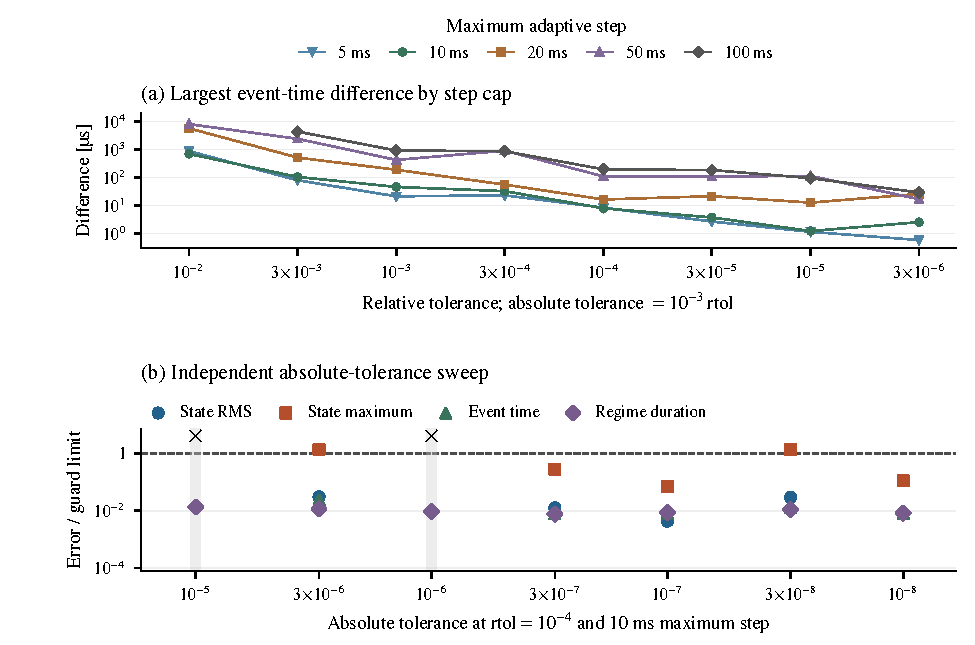
\includegraphics[width=\linewidth]{figures/results/verification/solver_acceptance_support.pdf}
  \caption{Additional control comparisons. Panel (a) identifies the five
  step caps underlying the event-time range in
  \Cref{fig:verification_solver_refinement}(c). The failed $10^{-2}$,
  \SI{100}{ms} combination has no ordinate. Lines connect tested settings.
  Panel (b) varies absolute tolerance alone. Each defined measure is divided
  by its own limit, so values above one fail that check. Crosses and grey
  strips denote different transition sequences, for which aligned state
  and corresponding-event measures are undefined. The regime-duration
  comparison remains defined in absolute time.}
  \label{fig:solver_acceptance_support}
\end{figure}
\FloatBarrier

Absolute tolerance sets the local-error scale near zero. It is therefore
varied separately at fixed $\mathrm{rtol}=10^{-4}$ and a \SI{10}{ms}
maximum step. In this sweep, $10^{-5}$ and $10^{-6}$ give
different transition histories. The $3\times10^{-6}$ and $3\times10^{-8}$
rows retain the reference history but exceed the maximum-state guard, with
shift-speed peaks of \SI{0.857448}{mm/s} and \SI{0.876497}{mm/s}.
The other three rows satisfy all checks. The nonmonotonic peak at
$3\times10^{-8}$ is retained as a measured sensitivity; its native history
was not archived, so no particular event or closure solve is assigned as
its cause. The main-grid intermediate row uses the proportional absolute tolerance
stored as $1.0000000000000001\times10^{-7}$, whereas the retained intermediate
cache uses literal $10^{-7}$. Their RMS values differ in late digits
($4.2741159\times10^{-7}$ and $4.2740764\times10^{-7}$). Figures and tables
retain those execution identities rather than combining their unrounded
metrics.

\paragraph{Separate gross-motion diagnostic and selected history.}
The exploratory population uses the archived absolute-time RMS for
$(\omega_p,\omega_s,v_b,s)$, omitting $\dot s$. Its combined value is the
square root of the mean of the four squared component RMS values, using
the scales above. Unlike the formal norm, it is an unweighted average over
the compact reference sample times. The original candidate trace has a
2 ms reporting spacing plus event endpoints and is linearly interpolated
onto that reference trace. Shared timestamps retain the outgoing state.
This compact diagnostic can therefore interpolate across a reset and
includes timing and reporting-grid effects. It is retained as a gross-motion
description, not used for formal hybrid acceptance or to infer a convergence
order. The plotted shift traces instead retain separate native segments.

\Cref{fig:solver_population_support} retains this exploratory comparison
and identifies the selected loose setting. Of 4,681 completed dense runs, 4,072 have the exact reference signature and
609 do not; 264 integrations fail. The latter completed group has a median
gross RMS of $1.2248411\times10^{-4}$ and a 90th percentile of
$3.493\times10^{-4}$. Sorting that group by gross RMS selects the middle
row at $\mathrm{rtol}=0.012684971009663653$,
$\mathrm{atol}=1.2684971009663654\times10^{-5}$ and
$\Delta t_{\max}=0.025041423884469123~\mathrm{s}$. Its trajectory was not
retained in the original dense archive, so those settings were replayed with
the installed frozen release and current study decoder. The replay reproduces
12 transitions and 486 native solver points, with gross RMS
$1.2249757\times10^{-4}$ rather than the archived $1.2248411\times10^{-4}$.
These are identified as separate executions; the replay supplies the displayed
history, not a claimed recovery of the original event timestamps.

\begin{figure}[!htb]
  \centering
  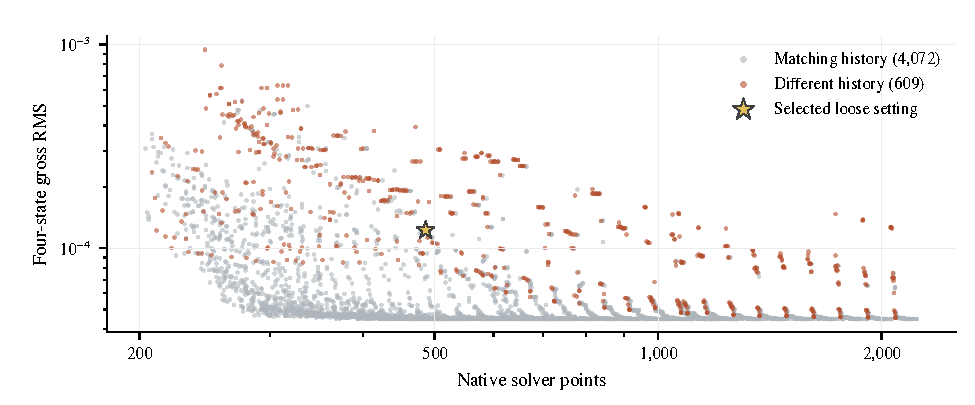
\includegraphics[width=\linewidth]{figures/results/verification/solver_population_support.pdf}
  \caption{Supplementary exploratory population and selection of the loose
  setting. The four-state compact gross-motion RMS is plotted against retained
  native solver points, with groups distinguished by their complete transition
  sequence. The star is the archived median among completed different-sequence
  calculations; its later replay supplies the resolved motion in
  \Cref{fig:verification_gross_hybrid_agreement}. Failed integrations have no
  trajectory norm and are excluded. This diagnostic omits shift speed and is
  not the formal five-state acceptance measure.}
  \label{fig:solver_population_support}
\end{figure}

\begin{table}[H]
\centering\small
\begin{tabular}{@{}crrr@{}}
\toprule
Excursion & Reference [$\mu$s] & Intermediate [$\mu$s] & Loose replay [$\mu$s] \\
\midrule
1 & 1878.269 & 1877.716 & 1412.204 \\
2 & 331.672 & 331.407 & 192.146 \\
3 & 60.418 & 60.292 & 7.219 \\
4 & 11.051 & 11.000 & --- \\
5 & 2.023 & 1.983 & --- \\
\bottomrule
\end{tabular}
\caption{Successive primary-separated intervals after first engagement and
before low-ratio seating. Dashes mean that no further excursion occurs, not
an interval of zero duration. The replay also retains a zero-duration engaged
segment at its final engagement/seating timestamp; neither event is discarded.}
\label{tab:solver_separation_intervals}
\end{table}

The seating marks in \Cref{fig:verification_gross_hybrid_agreement}
occur at \SI{66.012}{ms} (reference), \SI{66.004}{ms} (intermediate)
and \SI{64.830}{ms} (loose replay). The first separated excursions
reach sampled depths of \SI{49.016}{\micro\metre},
\SI{48.980}{\micro\metre} and \SI{22.326}{\micro\metre}, respectively.
The markers use the first outgoing low-ratio support event, not an
inference from the apparent flattening of the position trace.
The progressively shorter returns in
\Cref{tab:solver_separation_intervals} terminate under the fixed numerical
seating rule. They describe the retained implementation and are not offered
as independently resolved physical chatter. Their true durations are retained
in the segmentwise motion curves, including intervals narrower than a
display pixel; the full contact ledger remains in the retained evidence.

The small gross RMS is not a uniform dimensional bound. In the replay's
compact absolute-time comparison, the sampled maximum differences are
0.12045 rad/s in primary speed, 0.07551 rad/s in secondary speed,
0.21239 m/s in belt speed and 0.13422 mm in shift position. These maxima
include the differing event times and the reporting convention just described.
Native solver-point count likewise has a limited role: it sums retained
adaptive points over segments, including repeated boundary timestamps, and is
not a count of right-hand-side evaluations. In the archived formal execution,
the intermediate run retains 1,156 points and takes 7.257 s for hybrid
integration, compared with 4,451 points and 25.665 s for the tight reference.
The original machine is not identified, so these are within-execution
comparisons, not a portable speed claim or an optimal-setting result.

The maintained \texttt{solver-convergence/run.py} provides an archive-import
path, the selected-history replay and a checked \texttt{--plot-only} path.
Registered archive and member hashes identify the retained formal and dense
tables; both-side caches permit direct recomputation of the intermediate-run
metrics. The other per-point caches were not retained, so their tabulated
guards are rechecked without claiming a fresh integration or native-history
audit for every row. Exact replay inputs, numerical output hashes and the
original-versus-replayed distinction are recorded in
\ResultsCode{studies/solver-convergence/provenance/SECTION_4_2_3.md}{the study provenance note}.
\FloatBarrier

\section{Closure Conditioning and Root Structure}
\label{app:study_closure_conditioning}

The study separates the linear response at prescribed traction from the
nonlinear traction selection required by sticking. Its fixed-traction
condition number is \(\kappa_2(\vect A_s)\), where \(\vect A_s\) is the
row/column-equilibrated eight-variable matrix in
\Cref{eq:appendix_eight_unknown_closure,eq:appendix_equilibrated_system}.
The retained pulley torques are implementation unknowns; eliminating them
recovers the six-variable mechanical formulation. The sticking-root
Jacobian is a different object: the derivative of the frozen dimensional
relative-acceleration residuals with respect to the two tractions.
It is reconstructed by central differences at the reported root, using
\(h=10^{-5}\). The optimizer's working Jacobian is not substituted for
this derivative, because continuation can update that matrix from previous
states. Across all 15 roots, the relative spread in \(\kappa_2(\vect J_R)\)
over \(10^{-6}\leq h\leq3\times10^{-4}\) is at most
\(2.01\times10^{-6}\).

\subsection{Operating-State Maps and Starting-Guess Census}

The retained full run uses the configuration in
\ResultsCode{studies/closure-conditioning/study.json}{closure-conditioning/study.json}.
Four states come from the reference launch; eleven are constructed
stick--stick cases from the shared verification library. The low-ratio
seat, mid-shift, upper-stop and \texttt{free\_shift\_opening\_70} states
receive traction-plane maps. The last is a free opening state at \(70\%\)
engaged travel and \(-20~\mathrm{mm/s}\). The low-ratio seat already has
both the largest actual-root mechanical condition number and the largest
actual-root Jacobian condition number, so the worst-state selection adds
no fifth map.

\begin{table}[!htbp]
\centering\small
\begin{tabular}{@{}p{0.48\textwidth}p{0.44\textwidth}@{}}
\toprule
Quantity & Value \\ \midrule
Reference launch duration / reporting interval & 10 s / 2 ms \\
Reference launch rtol / atol / maximum step & $10^{-4}$ / $10^{-7}$ / 10 ms \\
Static / kinetic traction magnitudes & $\mu_s=0.65$ / $\mu_k=0.55$ \\
Static-box starting grid & $7\times7$ at each of 15 states \\
Expanded-box starting grid & $9\times9$ at each of four mapped states \\
Root-clustering distance & $10^{-6}$ in $(\lambda_p,\lambda_s)$ \\
\bottomrule
\end{tabular}
\caption{Retained full-run settings. Starting grids include their endpoints;
the expanded census is separate from the 735 static-box attempts.}
\label{tab:closure_study_settings}
\end{table}

\begin{table}[!htbp]
\centering\small
\begin{tabular}{@{}p{0.23\textwidth}p{0.18\textwidth}p{0.51\textwidth}@{}}
\toprule
Domain & Grid per state & Definition and scope \\ \midrule
Static capacity & $241\times241$ & $[-0.65,0.65]^2$, four states. Contact and support checks remain separate. \\
Expanded & $321\times321$ & $[-2.6,2.6]^2$, four states; mathematical continuation. \\
Broad & $501\times501$ & $[-10,10]^2$, mid-shift only; structural diagnostic. \\
\bottomrule
\end{tabular}
\caption{Retained traction domains. The expanded half-width is
$\max(2.5,4\mu_s)=2.6$. Map maxima are sampled values, not bounds between
grid points or condition numbers at the accepted roots.}
\label{tab:closure_lambda_domains}
\end{table}

All 644,488 sampled systems in the static and expanded maps have numerical
rank eight. This statement does not extend to the broad diagnostic: 76,746
of its 251,001 points are numerically rank deficient. The static-map maxima at the low-ratio seat, mid-shift, upper stop and
opening state are, respectively,
\(1.3260\times10^4\), \(3.6957\times10^4\), \(1.0540\times10^6\) and
\(8.2612\times10^3\). The upper-stop maximum occurs at
\((\lambda_p,\lambda_s)=(-0.216667,-0.254583)\); negative integrated
normal force, tension and local wrap-normal loading make that trial
inadmissible independently of the friction limits.

Every retained map includes signed normal resultants, minimum belt tension,
minimum local wrap-normal loading, an actuator-contact margin and the support
reaction. Its original mask includes the one-sided secondary-helix guard.
For the two maps in \Cref{fig:verification_closure_robustness}, the same mask
also applies to the bilateral reference: every rejected grid point independently
fails a belt-loading or support condition, while every accepted point passes
both original actuator-contact checks. Removing the secondary flank inequality
therefore changes neither plotted mask and does not discard a primary-contact
failure. There are 35,817 admissible points out of 58,081 at the upper stop,
and 51,198 at mid-shift. This equivalence is checked for these two maps only;
the historical masks of the other retained maps keep their original meaning.

The focused two-root field in \Cref{fig:verification_closure_fold} uses a
separate \(121\times161\) contact audit under the bilateral reference.
The primary-contact guard remains active. All 19,481 recalculated residual
pairs agree exactly with the retained field; 19,005 grid points pass the
contact checks. The dimensional residual norm is plotted on a logarithmic
colour scale, with the two signed components supplying their separate zero
contours. Cells touching a rejected point are excluded from these contours,
so an interpolated sign change across a contact-invalid region cannot appear
as a sticking solution. Root markers come from the corrected solutions, not
from interpolation of the colour field.

\begin{table}[!htbp]
\centering\small
\begin{tabular}{@{}lrrrr@{}}
\toprule
Frozen state & Accepted & Not accepted & $\kappa_2(A_s)$ & $\kappa_2(J_R)$ \\ \midrule
\texttt{low\_ratio\_seat} & 49 & 0 & $1.04\times10^4$ & 280 \\
\texttt{mid\_shift} & 42 & 7 & $9.44\times10^3$ & 22.8 \\
\texttt{late\_shift} & 42 & 7 & $8.02\times10^3$ & 28.0 \\
\texttt{upper\_stop} & 35 & 14 & $8.56\times10^3$ & 93.8 \\
\texttt{stick\_mid\_forward} & 49 & 0 & $1.57\times10^3$ & 1.97 \\
\texttt{stick\_mid\_reverse} & 49 & 0 & $1.57\times10^3$ & 1.97 \\
\texttt{stick\_low\_forward} & 42 & 7 & $5.90\times10^3$ & 21.8 \\
\texttt{stick\_high\_forward} & 46 & 3 & $2.52\times10^3$ & 4.68 \\
\texttt{stick\_mid\_stressed} & 45 & 4 & $1.82\times10^3$ & 6.62 \\
\texttt{free\_shift\_closing\_30} & 42 & 7 & $3.76\times10^3$ & 22.0 \\
\texttt{free\_shift\_closing\_50} & 49 & 0 & $1.62\times10^3$ & 2.39 \\
\texttt{free\_shift\_closing\_70} & 42 & 7 & $3.17\times10^3$ & 18.5 \\
\texttt{free\_shift\_opening\_30} & 42 & 7 & $3.83\times10^3$ & 20.3 \\
\texttt{free\_shift\_opening\_50} & 49 & 0 & $1.52\times10^3$ & 1.66 \\
\texttt{free\_shift\_opening\_70} & 43 & 6 & $3.62\times10^3$ & 13.6 \\
\midrule
Total & 666 & 69 & & \\
\bottomrule
\end{tabular}
\caption{All 735 static-box starts and condition numbers at the accepted
operating roots. Every state's accepted solutions form one cluster.
Forward/reverse and closing/opening cases remain distinct.}
\label{tab:closure_named_states}
\end{table}

Numerical acceptance requires optimizer success and the release's
sticking-compatibility checks. It does not itself certify every contact
inequality. Here the accepted solutions all lie within the static limits
and coincide, within the clustering tolerance, with the mechanically
accepted operating roots. The expanded census accepts 66, 27, 37 and 33 of
81 starts at the low-ratio seat, mid-shift, upper stop and opening state,
respectively. Thus 163 of 324 expanded starts are accepted, again in one
cluster per state, and none supplies an additional root. Unsuccessful
starts remain in both censuses. These finite searches neither exhaust
traction space nor establish global uniqueness.

All 69 rejected static-box searches returned optimizer success but failed
sticking compatibility. Their residual norms range from
\(13.31\) to \(424.36~\mathrm{m/s^2}\), compared with at most
\(3.10\times10^{-11}~\mathrm{m/s^2}\) for the accepted searches.
In 65 of them, the secondary traction reaches the numerical search bound
\(\lvert\lambda_s\rvert=1.95\); the other four terminate inside that
wider search interval. All 69 also exceed the physical secondary
static-friction limit. These are unsuccessful searches for a compatibility
root, rather than additional roots rejected only on physical grounds.
The retained rows do not include the optimizer's individual termination
messages. At the 15 accepted operating roots, the mechanical condition
number ranges from \(1.52\times10^3\) to \(1.04\times10^4\), indicating
substantially less numerical sensitivity than the rejected upper-stop
static-map maximum.
\FloatBarrier

\subsection{Selected Folded Branches}

The two-contact example in \Cref{fig:verification_closure_fold} fixes
position at \(95\%\) of engaged travel and shift speed at
\(-40~\mathrm{mm/s}\). Primary speed is \(3000~\mathrm{rpm}\);
secondary speed is \(3286.525553~\mathrm{rpm}\) and belt speed is
\(22.72382860~\mathrm{m/s}\), chosen to match both represented surfaces.
The attached primary and secondary bench inertias are
\(0.03\) and \(0.05~\mathrm{kg\,m^2}\), respectively. They are not the
nominal engine and vehicle boundaries. At the selected slice, the primary
boundary torque is \(-81.14811271~\mathrm{N\,m}\) and the secondary
boundary torque is \(+189.96446922~\mathrm{N\,m}\): with both shafts
rotating positively, the secondary boundary supplies power and the primary
boundary absorbs it.

\begin{table}[!htbp]
\centering\small
\begin{tabular}{@{}lrr@{}}
\toprule
Quantity & Root 1 & Root 2 \\ \midrule
Primary traction $\lambda_p$ & $-0.2676104653$ & $-0.3003678175$ \\
Secondary traction $\lambda_s$ & $+0.3340981242$ & $+0.5521247953$ \\
Primary normal resultant [N] & 3077.56 & 3122.29 \\
Secondary normal resultant [N] & 2400.85 & 1668.60 \\
Primary acceleration [rad/s$^2$] & $-575.334$ & $-346.401$ \\
Secondary acceleration [rad/s$^2$] & $+2919.426$ & $+2736.666$ \\
Belt acceleration [m/s$^2$] & $-72.4980$ & $-55.9388$ \\
Shift acceleration [m/s$^2$] & $+142.544$ & $+128.944$ \\
Minimum belt tension [N] & 174.100 & 170.668 \\
Minimum primary local normal loading [N/rad] & 65.7586 & 44.8540 \\
Minimum secondary local normal loading [N/rad] & 20.8365 & 0.242602 \\
$\kappa_2(A_s)$ & 6305.92 & 4364.80 \\
$\kappa_2(J_R)$ & 13.8870 & 27.5920 \\
\bottomrule
\end{tabular}
\caption{Retained frozen evaluation of the two traction pairs under installed
CINDER 1.1.2, at identical state and boundary torques. Both satisfy the
friction and mechanical-contact inequalities. The signed accelerations
show that the two roots define different local responses.}
\label{tab:closure_selected_roots}
\end{table}

The smaller static margin over both roots and interfaces is
\(\mu_s-|\lambda_j|=0.0978752\); it is not a normalized percentage.
Both fixed-traction matrices have rank eight. The checked
two-component sticking-residual norms are below
\(5.5\times10^{-11}~\mathrm{m/s^2}\). Each root's relative
\(\kappa_2(\vect J_R)\) spread over the same step range is below
\(1.57\times10^{-6}\).

The fixed-primary-torque branch is corrected from the retained inverse-grid
curve by solving both sticking residuals for \(\lambda_p\) and secondary
boundary torque at each prescribed \(\lambda_s\). The displayed open
segment has 184 points over \(0.30\leq\lambda_s\leq0.59\), including both
roots and the refined turn. Direct CINDER evaluation checks each point;
no endpoint is joined to the other. Its local maximum is
\(197.3901853~\mathrm{N\,m}\) at
\((\lambda_p,\lambda_s)=(-0.2856750,0.4134494)\),
\(7.4257161~\mathrm{N\,m}\) above the selected loading.
The turn is mechanically admissible and the fixed-traction matrix remains
rank eight throughout this segment. The root Jacobian becomes nearly
singular there, as expected when the traction response to loading turns;
this is a numerical local-extremum calculation, not an exact singularity
certificate. The dotted part of the curve has negative secondary local
wrap-normal loading and is excluded from the admissible branch.

The mixed example fixes the same travel fraction and opening speed but
uses \(2500~\mathrm{rpm}\) primary speed,
\(2736.737483~\mathrm{rpm}\) secondary speed and
\(18.93652384~\mathrm{m/s}\) belt speed. It retains the same bench
inertias. Boundary torques are \(-260~\mathrm{N\,m}\) primary and
\(+59.34019609~\mathrm{N\,m}\) secondary. With
\(\lambda_p=-\mu_k=-0.55\), the secondary sticking roots are
\(0.4342879568\) and \(0.5458610486\). Their scalar residual slopes
\(\partial R_s/\partial\lambda_s\) are approximately
\(+54.6254\) and \(-28.0426~\mathrm{m/s^2}\), respectively; a two-contact
Jacobian condition number is not used for this scalar problem.
Both roots have zero relative speed at the selected instant. Primary
relative accelerations of \(+364.835\) and
\(+379.770~\mathrm{m/s^2}\) have the required sign for onset of the
negative-traction slip branch. The secondary residual magnitudes are
below \(1.8\times10^{-10}~\mathrm{m/s^2}\).
Both roots pass the contact checks, although the minimum secondary local
normal loading falls from \(2.60109\) to
\(0.00616308~\mathrm{N/rad}\). The targeted search has 62 states and
15 candidate rows, but those rows represent one distinct state/branch
fold geometry under different fixed primary torques. They are not 15
independent fold discoveries or a frequency estimate.
\FloatBarrier

\subsection{Retained Evidence and Reproduction}

The earlier recap used \texttt{artifacts(10).zip}: 25 starts at each of
15 states, and \(81^2\), \(101^2\) and \(121^2\) maps. Its 375 attempts
and upper-stop static-map maximum \(3.38405\times10^5\) therefore do not
describe the full protocol above. The later retained
\texttt{artifacts(20260912-044618).zip} supplies the full census and maps;
no launch, broad map or multistart sweep was rerun for this finalization.
The selected folded branches come from separately registered targeted
archives. The two-contact curve's archived interpolated maximum,
\(197.4374~\mathrm{N\,m}\), is replaced by the locally corrected value
above, with both versions retained in the evidence.

The canonical
\ResultsCode{studies/closure-conditioning/run.py}{run.py}
provides a checked \texttt{--import-retained} path for the three original
archives and a \texttt{--plot-only} path for the delivered evidence.
The corrected roots and branch were recovered from the earlier finalization
package and verified against their registered hashes. This revision reuses
those calculations, all full maps and both starting-guess censuses. New
mechanical evaluations are limited to the focused contact grid above;
\texttt{--audit-contours} reproduces that check without a transient or
multistart search. Both execution records preserve exact input snapshots
and output hashes under installed \texttt{cinder-cvt==1.1.2}.
The newer live simulator is not imported.

Original archive/member hashes, the recovered package identity, numerical
checks and exact reproduction commands are recorded in
\ResultsCode{studies/closure-conditioning/provenance/SECTION_4_2_4.md}{the study provenance note}.
The retained archives do not contain a complete original machine and
dependency lock, so reproducing the plots and the selected frozen checks
does not establish bitwise regeneration of the historical full search.
\FloatBarrier

\section{Independent Ballew Benchmark}
\label{app:study_ballew}

Exact benchmark inputs supporting \Cref{sec:results_ballew_benchmark} are
defined in
\ResultsCode{studies/ballew-2015/study.json}{study.json}. The reconstruction
choices that translate Ballew's distributed-belt case into the quantities
required by CINDER are recorded in
\ResultsCode{studies/ballew-2015/provenance/RECONSTRUCTION.md}{RECONSTRUCTION.md}.
The benchmark assembly and shaft boundaries are constructed in
\ResultsCode{studies/ballew-2015/infrastructure/benchmark/case.py}{case.py},
with the source and reconstructed constants collected in
\ResultsCode{studies/ballew-2015/infrastructure/benchmark/constants.py}{constants.py}.
The comparison is model-to-model; the reference traces are Ballew's simulated
vehicle-acceleration results rather than experimental measurements.

\subsection{Source Data and Reconstruction}
\label{app:ballew_reconstruction}

The reconstruction retains Ballew's published pulley geometry, belt mass,
shaft inertias, vehicle data, initial shaft speeds, applied torque, secondary
clamp, and controller gains where they are reported. Quantities required by
CINDER but not specified by the source are introduced explicitly rather than
fitted to the digitized trajectories.

\begin{table}[H]
\centering
\small
\begin{tabular}{@{}p{0.48\textwidth}r@{}}
\toprule
Source-native quantity & Value \\
\midrule
Sheave half-angle & \(15^\circ\) \\
Pulley centre distance & \SI{0.2421}{\meter} \\
Published primary radius limits & \SIrange{0.0159}{0.0838}{\meter} \\
Published secondary radius limits & \SIrange{0.0159}{0.0838}{\meter} \\
One-dimensional belt length & \SI{0.8636}{\meter} \\
Belt mass & \SI{1.000}{\kilogram} \\
Primary pulley + engine inertia & \SI{0.008}{\kilogram\meter\squared} \\
Secondary pulley inertia & \SI{0.002}{\kilogram\meter\squared} \\
Secondary pulley + ATV inertia & \SI{1.275}{\kilogram\meter\squared} \\
Static / kinetic friction coefficients & \(0.55 / 0.40\) \\
Final-drive reduction & \(8.93\) \\
ATV mass & \SI{226}{\kilogram} \\
Tire radius & \SI{0.317}{\meter} \\
Rolling-resistance coefficient & \(0.048\) \\
Aerodynamic drag coefficient & \(1.0\) \\
Frontal area & \SI{1.39}{\meter\squared} \\
Primary applied torque & \SI{18}{\newton\meter} \\
Secondary closing force & \SI{2000}{\newton} \\
Initial primary / secondary speed & \(2500 / 1136~\mathrm{rpm}\) \\
Simulated interval & \SI{5}{\second} \\
\bottomrule
\end{tabular}
\caption{Source-native quantities retained in the Ballew reconstruction.}
\label{tab:ballew_source_quantities}
\end{table}

Ballew's transient belt is one-dimensional, whereas CINDER distinguishes the
outer belt geometry from the cord-line effective path. The reconstruction
identifies Ballew's published \SI{0.8636}{m} belt length with the CINDER
effective path. The smooth section taken from Ballew's Figure~39 is treated as
an equivalent load-carrying core with height \SI{7.62}{mm}, outer width
\SI{29.972}{mm}, inner width \SI{26.670}{mm}, and cord depth
\SI{1.270}{mm}. The corresponding CINDER outer length is
\SI{0.871579645}{m}. An effective density of
\SI{5316.543}{\kilogram\per\meter\cubed} then preserves the published
\SI{1.000}{kg} belt mass exactly. This density is a mass-preserving
reconstruction parameter, not a measured material density.

The published minimum radii are search limits rather than a simultaneously
compatible fixed-length endpoint. At the reconstructed low-ratio end, the
secondary effective radius is fixed at its published maximum,
\SI{0.0838}{m}, and belt-length closure gives the compatible primary effective
radius \SI{0.033647778}{m}. The always-engaged Ballew case uses zero deadzone
width, and the resulting CINDER shift range is \SI{0.026876495}{m}. Solving
within that geometry for the exact published shaft-speed ratio gives
\begin{equation}
\begin{aligned}
n_p(0)&=2500~\mathrm{rpm},&
n_s(0)&=1136~\mathrm{rpm},\\
s(0)&=\SI{0.001754497}{m},&
\dot s(0)&=0,\\
r_{p,\mathrm{eff}}(0)&=\SI{0.036921714}{m},&
r_{s,\mathrm{eff}}(0)&=\SI{0.081253771}{m},\\
v_b(0)&=\SI{9.666082}{m/s}.&&
\end{aligned}
\label{eq:ballew_reconstructed_initial_state}
\end{equation}

The two models use different normal-force conventions. Preserving the same
gross tangential capacity gives
\begin{equation}
\lambda=\frac{\mu\cos\beta}{2},
\label{eq:ballew_friction_translation}
\end{equation}
and therefore \(\lambda_s=0.2656296022\) and
\(\lvert\lambda_k\rvert=0.1931851653\) for \(\beta=15^\circ\).
This is a force-normalization translation rather than a friction fit.

The source traces are digitized from Ballew's Figures~41 and~45. Their raw
WebPlotDigitizer exports, project files, prepared CSVs, and the source thesis
are stored under
\ResultsCode{studies/ballew-2015/reference}{reference/}; file hashes are
recorded in
\ResultsCode{studies/ballew-2015/reference/manifest.json}{manifest.json}.
Preparation adds explicit headers, preserves the two native Figure~41 time
grids, averages exact duplicate Figure~45 timestamps, and extends the first
visible Figure~45 force back to \(t=0\) by zero-order hold. No smoothing,
filtering, curve fitting, or resampling is applied.

\subsection{Shaft Boundaries}
\label{app:ballew_boundaries}

Ballew publishes a combined primary-pulley/engine inertia, so the full
\SI{0.008}{\kilogram\meter\squared} is assigned to the primary shaft boundary
and is not duplicated inside the CVT. On the secondary side, CINDER owns the
published \SI{0.002}{\kilogram\meter\squared} output-pulley inertia. Vehicle
translation reflected through the fixed \(8.93\) reduction contributes
\SI{0.28478955}{\kilogram\meter\squared}; the remaining
\SI{0.98821045}{\kilogram\meter\squared} is carried as direct
secondary-boundary inertia so that the published
\SI{1.275}{\kilogram\meter\squared} output-pulley--ATV total is preserved.

\begin{table}[H]
\centering
\small
\begin{tabular}{@{}>{\raggedright\arraybackslash}p{0.47\textwidth}>{\raggedright\arraybackslash}p{0.17\textwidth}r@{}}
\toprule
Quantity & CINDER boundary & Value \\
\midrule
Primary applied torque \(\tau_{\mathrm{B},p}\) & Constant torque--inertia & \SI{18}{\newton\meter} \\
Primary referred inertia \(I_{\mathrm{B},p}\) & Constant torque--inertia & \SI{0.008}{\kilogram\meter\squared} \\
Final-drive reduction \(G\) & Locked final drive & \(8.93\) \\
Tire radius \(r_w\) & Locked final drive & \SI{0.317}{\meter} \\
ATV mass \(m_v\) & Locked final drive & \SI{226}{\kilogram} \\
Wheel rotational inertia \(I_w\) & Locked final drive & \SI{0}{\kilogram\meter\squared} \\
Rolling-resistance coefficient \(C_{rr}\) & Road load & \(0.048\) \\
Aerodynamic drag coefficient \(C_d\) & Road load & \(1.0\) \\
Frontal area \(A_f\) & Road load & \SI{1.39}{\meter\squared} \\
Road grade \(\gamma\) & Constant grade & \(0\) \\
Air density \(\rho\) & Reconstruction choice & \SI{1.225}{\kilogram\per\meter\cubed} \\
Gravity \(g\) & Reconstruction choice & \SI{9.80665}{\meter\per\second\squared} \\
Rolling-speed regularization \(v_\epsilon\) & Reconstruction choice & \SI{0.01}{\meter\per\second} \\
Reflected ATV translation \(m_v(r_w/G)^2\) & Locked final drive & \SI{0.28478955}{\kilogram\meter\squared} \\
Direct secondary-boundary inertia \(I_{s,\mathrm{dir}}\) & Locked final drive & \SI{0.98821045}{\kilogram\meter\squared} \\
Total secondary boundary inertia \(I_{\mathrm{B},s}\) & Locked final drive & \SI{1.273}{\kilogram\meter\squared} \\
\bottomrule
\end{tabular}
\caption{Shaft-boundary quantities used by the independent Ballew benchmark.}
\label{tab:ballew_boundary_values}
\end{table}

\subsection{Actuation and Host State}
\label{app:ballew_protocol_implementation}

The benchmark-specific axial-force laws are defined in
\Cref{app:ballew_actuator_implementations}. Both protocols retain the same
reconstructed geometry, inertias, friction translation, secondary clamp, and
vehicle boundary; only the primary clamping law differs.

\begin{table}[H]
\centering
\small
\begin{tabular}{@{}>{\raggedright\arraybackslash}p{0.18\textwidth}>{\raggedright\arraybackslash}p{0.29\textwidth}>{\raggedright\arraybackslash}p{0.22\textwidth}>{\raggedright\arraybackslash}p{0.23\textwidth}@{}}
\toprule
Protocol & Primary actuator & Secondary actuator & Host state \\
\midrule
Force replay & Prepared Figure~45 force history; piecewise-linear interpolation & Constant \SI{2000}{\newton} closing force & Secondary-shaft angle \\
Closed loop & PI force law of \Cref{eq:ballew_pi_force_law} & Constant \SI{2000}{\newton} closing force & Secondary-shaft angle and controller integral \(\eta\) \\
\bottomrule
\end{tabular}
\caption{Actuator and host configuration of the two Ballew benchmark protocols.}
\label{tab:ballew_actuator_protocols}
\end{table}

For the reconstructed closed-loop protocol, the controller uses
\(e=n_p-2500~\mathrm{rpm}\), \(K_{\mathrm{ff}}=1.2\), \(K_p=5\), and
\(K_i=75\). The feed-forward term is interpreted as
\(K_{\mathrm{ff}}F_{s,\mathrm{act}}=\SI{2400}{N}\), with \(\eta(0)=0\).
No saturation or anti-windup law is added because neither is specified by the
source.

\subsection{Numerical Settings}
\label{app:ballew_numerics}

\begin{table}[H]
\centering
\small
\begin{tabular}{@{}p{0.19\textwidth}p{0.12\textwidth}p{0.12\textwidth}p{0.13\textwidth}p{0.13\textwidth}p{0.10\textwidth}@{}}
\toprule
Protocol & \(\mathrm{rtol}\) & \(\mathrm{atol}\) & Max. step & Report step & Duration \\
\midrule
Force replay & \(10^{-7}\) & \(10^{-9}\) & 1 ms & 5 ms & 5 s \\
Closed loop & \(10^{-7}\) & \(10^{-9}\) & 1 ms & 0.2 ms & 5 s \\
\bottomrule
\end{tabular}
\caption{Numerical settings used by the two Ballew benchmark protocols.}
\label{tab:ballew_numerics}
\end{table}

Both protocols use LSODA, permit up to 2000 hybrid transitions, and retain
dense output. The separate closed-loop refinement check is defined in
\ResultsCode{studies/ballew-2015/provenance/NUMERICAL_STABILITY.md}{NUMERICAL_STABILITY.md}.

\begin{table}[H]
\centering
\small
\begin{tabular}{@{}lccc@{}}
\toprule
Refinement case & \(\mathrm{rtol}\) & \(\mathrm{atol}\) & Max. step \\
\midrule
Nominal & \(10^{-7}\) & \(10^{-9}\) & 1.00 ms \\
Nominal, refined step & \(10^{-7}\) & \(10^{-9}\) & 0.50 ms \\
Nominal, further refined step & \(10^{-7}\) & \(10^{-9}\) & 0.25 ms \\
Tighter tolerances & \(3\times10^{-8}\) & \(3\times10^{-10}\) & 0.50 ms \\
\bottomrule
\end{tabular}
\caption{Closed-loop numerical-refinement cases defined for the Ballew benchmark.}
\label{tab:ballew_refinement_settings}
\end{table}

All four cases complete the \SI{5}{s} interval. The reference errors remain
\(110.32~\mathrm{rpm}\) in primary speed, \(32.580~\mathrm{rpm}\) in secondary
speed and \SI{1196.25}{N} in primary clamp at the displayed precision.
To compare the actual trajectories, the solver's dense solution is evaluated
at common \SI{0.2}{ms} times within each continuous segment. Values are never
interpolated across an event; a time exactly on an event uses the outgoing
state. \Cref{tab:ballew_refinement_results} reports differences from the nominal
\SI{1}{ms} run, rather than differences from Ballew's reference.

\begin{table}[H]
\centering\small
\begin{tabular}{@{}lrrrr@{}}
\toprule
Case & \makecell{Primary speed\\RMS [rpm]} & \makecell{Primary clamp\\RMS [N]}
 & \makecell{Shift position\\max. [mm]} & \makecell{Matched event\\max. [\(\mu\)s]} \\
\midrule
Nominal, \SI{0.50}{ms} & 0.00942 & 0.0471 & 0.00384 & 0.513 \\
Nominal, \SI{0.25}{ms} & 0.01296 & 0.0649 & 0.00516 & 0.688 \\
Tighter, \SI{0.50}{ms} & 0.03203 & 0.1604 & 0.01258 & 1.673 \\
\bottomrule
\end{tabular}
\caption{Closed-loop refinement differences from the nominal \SI{1}{ms}
trajectory. Speed, clamp and position are compared at the same times over
\SIrange{0}{5}{s}; event times are matched by the ordered event records after
excluding slip-direction updates, as described below. The complete state and
event comparisons are retained in the publication evidence audit.}
\label{tab:ballew_refinement_results}
\end{table}

The raw event totals are \(1735\), \(1735\), \(1722\) and \(1421\), in the
order of \Cref{tab:ballew_refinement_settings}. They include \(320\), \(320\),
\(307\) and \(6\) zero-crossing updates of kinetic-slip direction. Excluding
only those updates leaves the same ordered \(1415\) event reasons and
incoming/outgoing sticking, sliding and support labels in all four runs.
These include \(207\) arrivals at the low-ratio seat. Their largest matched
timing difference is \SI{1.673}{\micro\second}. The large oscillations and
repeated seating therefore persist while the direction-update count is
sensitive to the integration settings.

Shift velocity requires care at those arrivals because it changes
instantaneously. At the common sample \(t=\SI{0.827}{s}\), the nominal run is
already seated while the \SI{0.25}{ms} and tighter-tolerance runs are still
arriving. The resulting same-time velocity difference is about
\SI{6.41}{m/s}; it compares opposite sides of the capture. Among common-grid
samples with matching contact and support labels, the largest shift-speed
difference across the refinements is \SI{0.00262}{m/s}. Event times and
continuous quantities are therefore reported separately, with both event
sides retained in the evidence.

The slip-loss curves integrate
\(\lvert(\tau_j/r_{j,\mathrm{eff}})v_{\mathrm{rel},j}\rvert\) separately on
each continuous segment. Reintegrating the retained power samples reproduces
the reported primary and secondary totals, \SI{12.3008}{kJ} and
\SI{7.4050}{kJ}. Retaining every second report sample, while keeping both
segment endpoints, changes their sum by \SI{7.98}{J}, or \(0.041\%\).
This sampling check supports the \SI{19.7}{kJ} scale used in the main text;
it is not a complete energy-balance or efficiency calculation.

\subsection{Reproduction and Retained Evidence}
\label{app:ballew_reproduction}

The benchmark and refinement runs use \texttt{cinder-cvt==1.1.2}, at the
simulator commit identified in \Cref{sec:results_implementation_reproducibility}. The
maintained study's
\ResultsCode{studies/ballew-2015/README.md}{README.md}
gives the environment setup and complete commands. From the repository root,
the canonical runner
\ResultsCode{studies/ballew-2015/run.py}{run.py}
accepts \texttt{--with-refinement} to run both protocols, the three additional
refinements and the evidence audit. Its \texttt{--plot-only} option reproduces
the final figures from retained inputs without repeating the simulations.

The exact executed source files, solver settings, reference hashes and output
hashes are recorded for every run. The
\ResultsCode{studies/ballew-2015/publication_inputs}{publication_inputs/}
directory retains compact plot and refinement arrays, selected without
resampling. Their
\ResultsCode{studies/ballew-2015/publication_inputs/publication_inputs.json}{checksum manifest}
identifies every retained file.
The full state and event exports accompany the manuscript delivery. The
publication plotter draws each continuous segment separately, including its
endpoints, and applies no smoothing. The audit recomputes the comparison
errors, checks the retained event sides and evaluates the refinement
quantities reported here.

\section{Common-Course Operation and Tuning}
\label{app:study_course_tuning}

Exact inputs supporting \Cref{sec:results_coupled_regimes} are defined by
\ResultsCode{studies/course-tuning/study.json}{study.json}. The selected road
and hardware cases are frozen in
\ResultsCode{studies/course-tuning/inputs/course.json}{course.json} and
\ResultsCode{studies/course-tuning/inputs/competitors.json}{competitors.json};
their selected-input hashes are recorded in
\ResultsCode{studies/course-tuning/inputs/selection.lock.json}{selection.lock.json}.
The maintained selection revision is
\texttt{section4p5-final-v3-r26b7-m170}.

All selected cases use CINDER~1.1.2, the reference CVT of
\Cref{app:common_physical_configuration}, the bilateral secondary-helix
topology of \Cref{app:reference_helix_topology}, the full-throttle primary
boundary of \Cref{app:primary_engine_boundary}, and the locked-final-drive
vehicle boundary of \Cref{app:secondary_vehicle_boundary}. They begin from the
common state in \Cref{eq:results_reference_initial_state}. The hardware
variants therefore change the CVT itself without changing the engine, vehicle,
belt/contact model, initial state, or numerical method.

\subsection{Distance-Indexed Road}
\label{app:course_profile}

Road position is signed travelled distance along the road surface. Constant
grades are joined by the \(C^2\) quintic transition
\begin{equation}
S(u)=u^3\left(10-15u+6u^2\right),
\qquad 0\le u\le1,
\label{eq:course_smoothstep}
\end{equation}
so a ramp from \(\gamma_0\) to \(\gamma_1\) over length \(L\) is
\(\gamma(x)=\gamma_0+(\gamma_1-\gamma_0)S((x-x_0)/L)\).
The cyclic region uses a \SI{12}{m}-wavelength sinusoidal grade with amplitude
\(32^\circ\), multiplied by the same smooth envelope over the first and last
\SI{6}{m}. The complete selected road is listed in
\Cref{tab:course_profile}.

\begin{table}[H]
\centering
\small
\begin{tabular}{@{}r r p{0.52\textwidth}@{}}
\toprule
Start [m] & End [m] & Road feature \\
\midrule
0 & 120 & Level launch and opening upshift \\
120 & 132 & Smooth \(0\rightarrow38^\circ\) entry \\
132 & 212 & Constant \(38^\circ\) climb \\
212 & 224 & Smooth \(38^\circ\rightarrow0\) exit \\
224 & 264 & Level recovery \\
264 & 336 & Six \SI{12}{m} cycles at \(\pm32^\circ\), zero mean, with \SI{6}{m} end envelopes \\
336 & 348 & Level separation \\
348 & 356 & Smooth \(0\rightarrow18^\circ\) entry \\
356 & 596 & Constant \(18^\circ\) climb \\
596 & 604 & Smooth \(18^\circ\rightarrow0\) exit \\
604 & 624 & Level recovery \\
624 & 636 & Smooth \(0\rightarrow-22^\circ\) descent entry \\
636 & 696 & Constant \(-22^\circ\) descent \\
696 & 708 & Smooth \(-22^\circ\rightarrow0\) exit \\
708 & 732 & Final level segment \\
\bottomrule
\end{tabular}
\caption{Distance-indexed road used by every selected common-course case.}
\label{tab:course_profile}
\end{table}

The road implementation is defined in
\ResultsCode{studies/course-tuning/infrastructure/course.py}{course.py}.
The signed distance is road arc length, so the elevation derivative is
\(\sin\gamma\), not \(\tan\gamma\). Full throttle is retained throughout; the
course changes only the road grade supplied to the secondary vehicle boundary.

\subsection{Selected Hardware Configurations}
\label{app:course_configurations}

The reference flyweight has a fixed arm/body mass of
\SI{13.646}{g} and a replaceable tip mass of \SI{250}{g} per flyweight.
Mass-scale cases change the tip mass and its associated first and second mass
moments consistently while leaving the arm/body mass unchanged. Spring-rate
case P300 triples the primary spring stiffness while choosing the installed
compression that preserves the reference spring force at the low-ratio
engagement geometry. The scalar actuator quantities resolved by
\ResultsCode{studies/course-tuning/infrastructure/tunes.py}{tunes.py} are
listed in \Cref{tab:course_resolved_actuation}.

\begin{table}[H]
\centering
\scriptsize
\setlength{\tabcolsep}{3.2pt}
\begin{tabular}{@{}lrrrrrr@{}}
\toprule
Case & Tip [g] & \(k_p\) [kN/m] & \(c_{p,0}\) [mm] & \(c_{s,0}\) [mm] & \(\theta_{s,\mathrm{pre}}\) [deg] & Helix [deg] \\
\midrule
R00 & 250.0 & 12.784 & 94.090 & 110.0 & 300 & 20 \\
W85 & 212.5 & 12.784 & 94.090 & 110.0 & 300 & 20 \\
P300 & 250.0 & 38.352 & 29.704 & 110.0 & 300 & 20 \\
RC10 & 250.0 & 12.784 & 94.090 & 110.0 & 300 & 20 \\
R26B7 & 250.0 & 12.784 & 94.090 & 110.0 & 300 & 20 \\
RC40L & 250.0 & 12.784 & 94.090 & 110.0 & 300 & 20 \\
H28 & 250.0 & 12.784 & 94.090 & 110.0 & 300 & 28 \\
U55 & 137.5 & 12.784 & 94.090 & 110.0 & 300 & 20 \\
D01 & 325.0 & 12.784 & 75.272 & 88.0 & 240 & 28 \\
D02 & 162.5 & 12.784 & 108.204 & 110.0 & 300 & 20 \\
D02\_M & 250.0 & 12.784 & 108.204 & 110.0 & 300 & 20 \\
D02\_M170 & 425.0 & 12.784 & 108.204 & 110.0 & 300 & 20 \\
D02\_P & 162.5 & 12.784 & 94.090 & 110.0 & 300 & 20 \\
\bottomrule
\end{tabular}
\caption{Resolved scalar actuator quantities for the thirteen selected
common-course configurations. \(c_{p,0}\) and \(c_{s,0}\) are installed axial
spring compressions. The helix angle is measured from the circumferential
direction. Unlisted actuator quantities retain the R00 reference values.}
\label{tab:course_resolved_actuation}
\end{table}

The three selected ramp cases retain the same fixed-pivot hardware and
flyweight mass properties as R00. Only the contacted ramp profile is changed.
The baseline profile consists of a \SI{5}{mm} linear \(35^\circ\) segment, a
\SI{3}{mm} \(C^3\) blend, and a \SI{30}{mm} circular segment from
\(35^\circ\) to \(20^\circ\). The selected modifications are

\begin{table}[H]
\centering
\small
\begin{tabular}{@{}lrrr@{}}
\toprule
Case & Unchanged prefix [mm] & \(C^3\) blend [mm] & Arc-tail end angle \\
\midrule
RC10 & 10 & 5 & \(10^\circ\) \\
R26B7 & 10 & 7 & \(26^\circ\) \\
RC40L & 18 & 5 & \(40^\circ\) \\
\bottomrule
\end{tabular}
\caption{Selected primary-ramp modifications used on the common course. The
prefix and blend distances are physical coordinates along the ramp, not
movable-sheave travel.}
\label{tab:course_ramp_variants}
\end{table}

All other selected cases retain the baseline ramp. In particular,
\texttt{D02\_M} restores the reference tip mass while retaining D02's
\(115\%\) primary preload, \texttt{D02\_P} restores the reference primary
preload while retaining D02's \(65\%\) tip mass, and
\texttt{D02\_M170} uses \(170\%\) tip mass while retaining the \(115\%\)
primary preload. No quasi-static actuator replacement, force scaling, or
fitted speed curve is introduced in these course cases.

\subsection{Numerical and Stopping Controls}
\label{app:course_numerics}

The selected common-course study runs thirteen cases on the \SI{732}{m} road
and two supporting cases, R00 and U55, on a separate \SI{800}{m} flat road.
All fifteen trajectories use the same tight numerical settings.

\begin{table}[H]
\centering
\small
\begin{tabular}{@{}p{0.55\textwidth}r@{}}
\toprule
Setting & Value \\
\midrule
Integrator & LSODA \\
Relative tolerance & \(3\times10^{-5}\) \\
Absolute tolerance & \(3\times10^{-8}\) \\
Maximum integration step & \SI{5}{ms} \\
Diagnostic/report interval & \SI{5}{ms} \\
Maximum simulated time & \SI{180}{s} \\
Maximum total hybrid transitions & 5000 \\
Checkpoint interval & \SI{2}{s} \\
Maximum transitions per checkpoint & 600 \\
Event-time tolerance & \(10^{-10}~\mathrm{s}\) \\
Per-case wall timeout & \SI{1800}{s} \\
Progress monitor begins after & \SI{20}{s} \\
No-progress review window & \SI{15}{s} \\
Minimum progress over review window & \SI{0.25}{m} \\
Rollback stop speed & \SI{-0.25}{m/s} \\
\bottomrule
\end{tabular}
\caption{Numerical and execution controls of the selected common-course study.}
\label{tab:course_numerics}
\end{table}

A progress or rollback stop is recorded as a physical observed outcome of the
specified case rather than as a numerical or model-domain failure. Conversely,
integration, construction, or model-domain errors remain distinct stopping
classes. The runner does not restart a sector from a prescribed state: each
common-course trajectory is continuous from the shared initial condition until
completion or its recorded stopping condition.

The separate \SI{800}{m} flat experiment uses the same numerical settings and
contains only R00 and U55. It is a supporting test of whether U55's incomplete
opening shift on the common course is merely caused by the first hill arriving
at \SI{120}{m}; it is not appended to the common road and does not alter the
selected course.

\subsection{Settling and Archived Case Records}
\label{app:course_reporting}

Interior settling checks use a \SI{5}{s} window advanced in
\SI{0.25}{s} increments. A candidate window must remain at least
\SI{0.25}{mm} from either shift stop, maintain forward speed above
\SI{0.1}{m/s}, and remain on constant grade. The principal variation limits
are listed in \Cref{tab:course_settling_criteria}; the complete criteria are
defined in
\ResultsCode{studies/course-tuning/inputs/settling_criteria.json}{settling_criteria.json}.

\begin{table}[H]
\centering
\small
\begin{tabular}{@{}p{0.62\textwidth}r@{}}
\toprule
Settling criterion & Limit \\
\midrule
Maximum \(\lvert\dot s\rvert\) & \SI{0.05}{mm/s} \\
Maximum vehicle acceleration magnitude & \SI{0.01}{m/s^2} \\
Maximum primary RPM rate magnitude & \(2~\mathrm{rpm/s}\) \\
Maximum secondary RPM rate magnitude & \(2~\mathrm{rpm/s}\) \\
Maximum belt acceleration magnitude & \SI{0.01}{m/s^2} \\
Maximum shift acceleration magnitude & \SI{5e-4}{m/s^2} \\
Shift range within window & \SI{0.1}{mm} \\
Vehicle-speed range within window & \SI{0.05}{m/s} \\
Primary-speed range within window & \(10~\mathrm{rpm}\) \\
Secondary-speed range within window & \(10~\mathrm{rpm}\) \\
Belt-speed range within window & \SI{0.05}{m/s} \\
\bottomrule
\end{tabular}
\caption{Principal finite-window settling criteria used by the common-course
analysis. Passing a window establishes only the stated finite-window
condition.}
\label{tab:course_settling_criteria}
\end{table}

The final study output is self-describing. The top-level
\texttt{suite.json} records the selected study identity, numerical controls,
and environment. Each case stores a complete \texttt{resolved\_case.json},
\texttt{model\_identity.json}, event history, sampled diagnostics, and stopping
summary. The common-course report also stores the resolved physical tune table
and the analytic road sectors. The intended appendix-facing inventory is
summarized in
\ResultsCode{studies/course-tuning/provenance/APPENDIX_HANDOFF.md}{APPENDIX_HANDOFF.md}.
These records, rather than the human-readable case labels, define the exact
simulation inputs used by the study.

\end{document}